\documentclass[12pt,a4paper,openany]{book}
\usepackage{fullpage}
\usepackage[utf8]{inputenc}
\usepackage{amsmath,amsfonts,amsthm}
\usepackage[spanish]{babel}
\usepackage{enumerate}
\usepackage{graphicx,psfrag}
\usepackage{tikz}
% \usepackage{pgfplots}
\usepackage{stackengine}
\usepackage{xcolor}
\usepackage{comment}
\usepackage{array}
\usepackage{color}
\usepackage{srcltx}
\usepackage{todonotes}
\usepackage{multicol}
\usepackage{xspace}
\usepackage{stackengine}
\usepackage[%
%   pdftex=true,  % si se usa pdftex
   pdfpagemode=UseNone,
breaklinks=true,
%   pdfstartpage=3,   % para empezar en pag. 3
   bookmarks=true,
%   bookmarksopen=true,
%   bookmarksnumbered=true,
%   plainpages=false, % cuando existe p\'agina i y p\'agina 1
%   pdfstartview=XYZ,
%   pdfpagelabels=true, % ii en preambulo
%   pagebackref=true, % referencias a citas
   colorlinks,
   linkcolor=blue,% cambiar a black para imprimir
%   linktocpage, % link en el n\'umero de pagina en toc
   anchorcolor=blue,
   citecolor=black,% cambiar a black para imprimir
   filecolor=blue,
%    pagecolor=blue,
   urlcolor=blue
   ]{hyperref}

\usepackage{etoolbox}
\newcommand\getcurrentref[1]{%
 \ifnumequal{\value{#1}}{0}
  {??}
  {\the\value{#1}}%
}    

\usepackage{cancel}
%\newcounter{savectr}
%\newcommand{\savectr}[1]{\setcounter{savectr}{\value{#1}}}
%\newcommand{\backctr}[1]{\setcounter{#1}{\value{savectr}}}
\newcounter{contadorejemplo}
%\newcommand{\ejemplo}{\medskip\textbf{Ejemplo \arabic{contadorejemplo}:} \addtocounter{contadorejemplo}{1}}
%\setcounter{contadorejemplo}{1}
%\DeclareGraphicsExtensions{eps}

\newcommand{\comentario}[1]{{\begin{quote}\small\color{gray}#1\end{quote}}}


\newcommand{\completar}[1]{\todo[inline]{Completar. {#1}}}
\newcommand{\sucan}{\ensuremath{\left(a_n\right)_{n\in\N}}\xspace}
\newcommand{\sucxn}{\ensuremath{\left(x_n\right)_{n\in\N}}\xspace}
\newcommand{\sucyn}{\ensuremath{\left(y_n\right)_{n\in\N}}\xspace}
\newcommand{\sucSn}{\ensuremath{\left(S_n\right)_{n\in\N}}\xspace}
\newcommand{\serieak}{\ensuremath{\sum_{k=1}^\infty a_k}\xspace}
\newcommand{\seriean}{\ensuremath{\sum_{n=1}^\infty a_n}\xspace}
\newcommand{\seriebk}{\ensuremath{\sum_{k=1}^\infty b_k}\xspace}
\newcommand{\seriebn}{\ensuremath{\sum_{n=1}^\infty b_n}\xspace}
\newcommand{\subsucan}{\ensuremath{\left(a_{n_k}\right)_{k\in\N}}\xspace}
\newcommand{\sucbn}{\ensuremath{\left(b_n\right)_{n\in\N}}\xspace}
\newcommand{\succn}{\ensuremath{\left(c_n\right)_{n\in\N}}\xspace}
\newcommand{\niN}{{\ensuremath{n\in\N}}\xspace}
\newcommand{\xiR}{{\ensuremath{x\in\R}}\xspace}
\newcommand{\xoiR}{{\ensuremath{x_0\in\R}}\xspace}
\newcommand{\limxo}{{\ensuremath{\lim_{x\to x_0}}}}
\newcommand{\limho}{{\ensuremath{\lim_{h\to 0}}}}
\newcommand{\limxop}{{\ensuremath{\lim_{x\to x_0^+}}}}
\newcommand{\limxom}{{\ensuremath{\lim_{x\to x_0^-}}}}
\newcommand{\ton}{\stackunder{\ $\longrightarrow$\ }{\scriptsize$n\to\infty$}}
\newcommand{\tox}[1]{\stackunder{\ $\longrightarrow$\ }{\scriptsize$x\to{#1}$}}
\newcommand{\toy}[1]{\stackunder{\ $\longrightarrow$\ }{\scriptsize$y\to{#1}$}}
\newcommand{\toh}[1]{\stackunder{\ $\longrightarrow$\ }{\ \scriptsize$h\to{#1}$\ }}
\newcommand{\eqLH}{\stackon{\,=}{\,\,\scriptsize{(L'H)}}\,\,}
\newcommand{\note}[1]%
{\noindent\centerline{\fbox{\parbox{.9\textwidth}{\textbf{#1}}}}}
\newcommand{\snote}[1]%
{\fbox{\textbf{#1}}}

% \theoremstyle{plain}
\parskip=10pt
\usepackage{thmtools}

\declaretheoremstyle[
  shaded={rulecolor=black, rulewidth=0.7pt, bgcolor=white, 
  textwidth=.95\textwidth, padding=6pt, leftmargin=5pt},
  spaceabove=6pt, spacebelow=6pt,
]{miestilo}
\declaretheorem[
  style=miestilo,
  name=Teorema,
  numberwithin=chapter,
  ]{theorem}
\declaretheorem[
    style=miestilo,
  name=Lema,
  numberlike=theorem,
  ]{lemma}
\declaretheorem[
    style=miestilo,
  name=Corolario,
  numberlike=theorem,
]{corollary}
\declaretheorem[
    style=miestilo,
    name=Proposición,
  numberlike=theorem,
  ]{proposition}
\declaretheorem[
    style=miestilo,
    name=Definición,
  numberlike=theorem,
  ]{definition}
%    \newtheorem{theorem}{Teorema}[chapter]
%    \newtheorem{lemma}[theorem]{Lema}
%    \newtheorem{corollary}[theorem]{Corolario}
%    \newtheorem{proposition}[theorem]{Proposición}

\theoremstyle{definition}
   \newtheorem{remark}[theorem]{Observación}
   \newtheorem{example}[theorem]{Ejemplo}
%    \newtheorem{definition}[theorem]{Definición}
%    \newtheorem{pb}{ }[chapter]
%    \newtheorem{pbm}[pb]{*}
%    \newtheorem{pbo}[pb]{**}

\usepackage{attachfile2}

%\usepackage{matlab-prettifier}
\usepackage{listings}
\lstset{
  basicstyle=\ttfamily,
  columns=fixed,
  fontadjust=true,
  basewidth=0.5em,
  frame=single,
  float=h!
}

%\lstset{language=Octave,basicstyle=\ttfamily}
\newcommand{\includescript}[2]{\lstinputlisting[title={Script \texttt{#2}. \attachfile{#1/#2}}]{#1/#2}}

\newcommand{\includefunction}[2]{\lstinputlisting[title={Función \texttt{#2}. \attachfile{#1/#2}}]{#1/#2}}


\newcommand{\recuadro}[1]%
{\medskip\noindent\centerline{\fbox{\parbox{.97\textwidth}{\medskip\centerline{\parbox{.95\textwidth}{#1}}\medskip}}}\medskip}

\DeclareMathOperator{\sgn}{sgn}
\DeclareMathOperator{\cotan}{cotan}
\DeclareMathOperator{\cosec}{cosec}
\DeclareMathOperator{\Dom}{Dom}
\DeclareMathOperator{\dom}{Dom}
\DeclareMathOperator{\im}{Im}

\DeclareMathOperator{\SF}{SF}
\newcommand{\SFS}{\SF^s}
\newcommand{\SFC}{\SF^c}
\DeclareMathOperator{\vol}{vol}
\DeclareMathOperator{\length}{longitud}
\newcommand{\area}{\mathrm{\protect\acute{a}rea}}
\newcommand{\dvol}{\,d\mathrm{vol}}
\newcommand{\dA}{\,dA}
\newcommand{\dx}{\,dx}
\newcommand{\dy}{\,dy}
\newcommand{\dz}{\,dz}
\newcommand{\ds}{\,ds}
\newcommand{\dr}{\,dr}
\newcommand{\dtheta}{\,d\theta}
\newcommand{\dsv}{\cdot d\ol{s}}
\newcommand{\dS}{\,d\sigma}
\newcommand{\dt}{\,dt}
\newcommand{\du}{\,du}
\newcommand{\dv}{\,dv}
\newcommand{\LL}{\mathcal{L}}
\DeclareMathOperator{\di}{div}
\DeclareMathOperator{\proy}{Proy}
\DeclareMathOperator{\Circ}{Circ}
%\usepackage[notcite,notref]{showkeys}
\newcommand{\Chi}{\raise2pt\hbox{$\chi$}}

\newcommand{\pedro}{}
\newcommand{\eps}{\varepsilon}
\newcommand{\F}{\mathcal{F}}
\newcommand{\R}{\mathbb{R}}
\newcommand{\C}{\mathbb{C}}
\newcommand{\V}{\mathbb{V}}
\newcommand{\N}{\mathbb{N}}
\newcommand{\Q}{\mathbb{Q}}
\newcommand{\Z}{\mathbb{Z}}
\newcommand{\D}{\displaystyle}
\newcommand{\gr}{^{\text{o}}}
\newcommand{\ux}{\D\frac{\partial u}{\partial x}}
\newcommand{\uy}{\D\frac{\partial u}{\partial y}}
\newcommand{\uxx}{\D\frac{\partial^2 u}{\partial x^2}}
\newcommand{\uyy}{\D\frac{\partial^2 u}{\partial y^2}}
\newcommand{\uzz}{\D\frac{\partial^2 u}{\partial z^2}}
\newcommand{\phixx}{\phi_{xx}}
\newcommand{\phiyy}{\phi_{yy}}
\newcommand{\phizz}{\phi_{zz}}
\newcommand{\phin}{\phi_n}
\newcommand{\phinm}{\phi_{n\,m}}
\newcommand{\phikl}{\phi_{k\,\ell}}
\newcommand{\lambdanm}{\lambda_{n\,m}}
\newcommand{\znm}{z_{n\,m}}
\newcommand{\anm}{a_{n\,m}}
\newcommand{\bnm}{b_{n\,m}}
\newcommand{\fnm}[1][]{f_{n\,m_{#1}}}
\newcommand{\ut}{\D\frac{\partial u}{\partial t}}
\newcommand{\vphi}{\boldsymbol{\phi}}
\newcommand{\enf}{\textbf}
\newcommand{\nn}{\ol{n}}
\newcommand{\pd}[3][]{\D\frac{\partial^{#1} {#2}}{\partial #3^{#1}}}
\newcommand{\dd}[3][]{\frac{d^{#1} {#2}}{d #3^{#1}}}
\newcommand{\grad}{\nabla}
\newcommand{\ii}{\ol{i}}
\newcommand{\jj}{\ol{j}}
\newcommand{\kk}{\ol{k}}
\DeclareMathOperator{\sop}{sop}

\newcommand{\esp}{\R^3}
\newcommand{\obs}{\Theta}
\newcommand{\ol}{\overline}
\newcommand{\ul}{\underline}
\newcommand{\oll}[1]{\ol{\ol #1}}
\newcommand{\olll}[1]{\ol{\ol{\ol #1}}}
\newcommand{\inv}{^{-1}}
\newcommand{\olnabla}{\ol\nabla}

% \newcommand{\mara}[1]{{\color{blue}#1}}
% \newcommand{\mauri}[1]{{\color{brown}#1}}
% \newcommand{\sofi}[1]{{\color{cyan}#1}}
\newcommand{\mara}[1]{{#1}}
\newcommand{\mauri}[1]{{#1}}
\newcommand{\sofi}[1]{{#1}}

\title{Cálculo I}


\author{
Apunte de la materia\\[6pt]
\emph{Cálculo I} \\[6pt]
de las carreras\\[6pt]
Licenciatura en Ciencia de Datos\\
Licenciatura en Matemática Aplicada\\[6pt]
Facultad de Ingeniería Química\\[12pt]
Universidad Nacional del Litoral
\\
Pedro Morin
}

\begin{document}
\maketitle

\chapter*{Presentación}
Este apunte contiene las notas del curso \emph{Cálculo I}, que se dicta simultáneamente para las carreras de Licenciatura en Matemática Aplicada y Licenciatura en Ciencia
de Datos, en la Facultad de Ingeniería Química de la Universidad Nacional
del Litoral.

En la sección Ejercicios de cada sección y capítulo hay problemas marcados con un asterisco. Estos problemas más teóricos están pensados para los alumnos de Licenciatura en Matemática Aplicada.

\bigskip

Este apunte fue escrito durante el dictado del curso en el segundo cuatrimestre de 2024, y será actualizado durante futuros dictados de la asignatura.
Cualquier sugerencia u observación sobre errores será agradecida por el autor del apunte y también por los futuros alumnos del curso.

\bigskip
\bigskip
\bigskip

\hfil\hfil\hfil Santa Fe, agosto 2024.


\tableofcontents

\chapter{Repaso de Números Reales}
\label{Cap:Reales}

\section{Propiedades de cuerpo ordenado}

Recordamos a continuación los axiomas de cuerpo ordenado que cumple el conjunto $\R$ de los números reales.

Las propiedades básicas de la suma son cuatro:

\begin{description}
    \item[$S_1$. Conmutatividad de la suma:] Cualesquiera sean los números reales $a$ y $b$ vale
    \[ a+b = b+a.\]

    \item[$S_2$. Asociatividad de la suma:] Cualesquiera sean los números reales $a$, $b$ y $c$, vale
    \[
    a + (b+c) = (a+b) + c.
    \]

    \item[$S_3$. Existencia de elemento neutro para la suma:] Existe un número real llamado \emph{cero} y que indicamos 0 tal que, para todo número real $a$ vale:
    \[ a+0 = a.\]

    \item[$S_4$. Existencia del inverso aditivo:] Dado un número real $a$, existe un número real que llamamos \emph{inverso aditivo de $a$} o también \emph{opuesto de $a$}, e indicamos $-a$ tal que
    \[ a+(-a) = 0.\]

\end{description}

Las propiedades básicas del producto son también cuatro, y se corresponden exactamente con las de la suma:

\begin{description}
    \item[$P_1$. Conmutatividad del producto:] Cualesquiera sean los números reales $a$ y $b$ vale
    \[ a\cdot b = b\cdot a.\]

    \item[$P_2$. Asociatividad del producto:] Cualesquiera sean los números reales $a$, $b$ y $c$, vale
    \[
    a \cdot (b \cdot c) = (a \cdot b) \cdot c.
    \]

    \item[$P_3$. Existencia de elemento neutro para el producto:] Existe un número real distinto de cero, llamado \emph{uno} y que indicamos 1 tal que, para todo número real $a$ vale:
    \[ a \cdot 1 = a.\]

    \item[$P_4$. Existencia del inverso multiplicativo:] Dado un número real $a$, distinto de cero, existe un número real que llamamos \emph{inverso multiplicativo de $a$} o también \emph{recíproco de $a$}, e indicamos $a\inv$ tal que
    \[ a \cdot a\inv = 1.\]

\end{description}

También tenemos una propiedad que vincula la suma con el producto:

\begin{description}
    \item[$D$. Propiedad distributiva:] Cualesquiera sean los números reales $a$, $b$ y $c$ vale:
    \[ a\cdot(b+c) = a\cdot b+a\cdot c.\]
\end{description}

Finalmente, existe en los números reales un \emph{orden}. La notación $a<b$ significa
\emph{$a$ es menor que $b$} y es exactamente lo mismo que $b>a$, que se lee \emph{$b$ es mayor que $a$}. Para el orden, tenemos las siguientes propiedades:

\begin{description}
    \item[$O_1$. Tricotomía:] Si $a$ y $b$ son números reales, vale una y sólo una de las siguientes posibilidades:
    \[
    a<b,\qquad a=b, \qquad a>b.
    \]

    \item[$O_2$. Transitividad:] Si $a$, $b$ y $c$ son números reales que verifican
    \[ a<b \qquad\text{y}\qquad b<c\]
    entonces necesariamente \ $a<c$.

    \item[$O_3$. Monotonía de la suma:] Si $a$ y $b$ son números reales que verifican
    \[ a<b, \]
    entonces cualquiera sea el número real $c$ vale:
    \[ a+c < b+c.\]

    \item[$O_4$. Monotonía del producto:] Si $a$ y $b$ son números reales que verifican
    \[ a<b, \]
    entonces cualquiera sea el número real $c$ mayor que cero vale:
    \[ a \cdot c < b \cdot c.\]


\end{description}

\mauri{Se puede probar como ejercicio que 
$a < b$ si y solo si $-b < -a$, con lo cual, 
por la propiedad $O_4$ anterior tenemos que:
Si $a$ y $b$ son números reales que verifican
    \[ a<b, \]
    entonces cualquiera sea el número real $c$ menor que cero vale:
    \[ a \cdot c > b \cdot c.\]}

Recordamos algunas propiedades que se deducen de estos axiomas:

\begin{description}
    \item[Propiedad cancelativa para la suma:] Si $a$, $b$ y $c$ son números reales tales que
    \[ a+c = b+c\]
    entonces \ $a=b$.

    \item[Unicidad del cero:] Si $a$ y $b$ son números reales tales que
    \[a+b=a,\]
    entonces debe ser \ $b=0$.

    \item[$a\cdot 0 = 0$:] Cualquiera sea el número real $a$, vale que $a\cdot 0 = 0$.

    \item[Propiedad cancelativa para el producto:] Si $a$, $b$ y $c$ son números reales tales que $c\neq 0$ y
    \[ a\cdot c = b \cdot c\]
    entonces \ $a=b$.

    \item[Reglas de los signos:]
    \begin{itemize}
        \item Si $a$ es un número real, entonces \ $-(-a) = a$.
        \item Si $a$ y $b$ son números reales, entonces \ $(-a)\cdot b = -(a\cdot b)$.
        \item Si $a$ y $b$ son números reales, entonces \ $(-a)\cdot (-b) = a\cdot b$.
    \end{itemize}

    \item[Por último: $0<1$.]
\end{description}

Finalmente, decimos que $a$ es menor o igual a $b$, y escribimos $a\le b$, cuando $a<b$ o $a=b$.

\subsubsection*{Ejercicios de la sección~\getcurrentref{chapter}.\getcurrentref{section}}

\begin{enumerate}
    
    \item Probar que si $a,b,x,y \in \R$, $a<b$ y $x<y$, entonces $a+x < b+y$.

    \item Probar que si $a,b\in\R$ y $a<b$, entonces $\D a<\frac{a+b}2<b$.

    \item Verificar que:
    \begin{enumerate}
        \item $n < n + 5 < 2 n$, para todo $n\in\N$, $n > 5$.
        \item $n < n + 5 < 2 n$, para todo $n\in\N$, $n > 50$.
        \item $\frac n2 < n - 10 < n$, para todo $n\in\N$, $n > 20$.
        \item $\frac n2 < n - 10 < n$, para todo $n\in\N$, $n > 100$.
        \item $5\, n^2 < 5\,n^2 + n - 5 < 6\, n^2$, para todo $n\in\N$, $n > 5$.
        \item $4\, n^2 < 5\,n^2 - n  < 5\, n^2$, para todo $n\in\N$, $n > 5$.
    \end{enumerate}

    \item Hallar $N_0\in\N$ tal que:
    \begin{enumerate}
        \item $n < n + 30 < 2 n$, para todo $n\in\N$, $n > N_0$.
        \item $\frac n2 < n - 30 < n$, para todo $n\in\N$, $n > N_0$.
        \item $5\, n^2 < 5\,n^2 + n - 5 < 6.1\, n^2$, para todo $n\in\N$, $n > N_0$.
        \item $4.9\, n^2 < 5\, n^2 - n  < 5\, n^2$, para todo $n\in\N$, $n > N_0$.
        \item $n^2 < 2\,n^2 - 10\, n + 8 < 3\, n^2$, para todo $n\in\N$, $n > N_0$.
        \item $2\, n^3 < 3\,n^3 - 5 n^2 + 30 < 3\, n^3$, para todo $n\in\N$, $n > N_0$.
    \end{enumerate}


\end{enumerate}

\section{Cotas superiores e inferiores, máximo y mínimo}

\begin{definition}
    Dado un conjunto $A$ de números reales, se dice que $c$ es una cota inferior de $A$ si
    \[
    c \le a,\qquad \forall a\in A.
    \]
    Es decir, un número real es una cota inferior de un conjunto cuando es menor o igual que todos los elementos del conjunto.
\end{definition}

\begin{itemize}
\item Existen conjuntos que no tienen cotas inferiores. Pensar ejemplos.
\item Si $c$ es una cota inferior, entonces todos los elementos de $(-\infty,c]$ son cotas inferiores. Demostrar
\item Si un conjunto tiene una cota inferior, se dice que es \emph{acotado inferiormente}.
\end{itemize}

\begin{definition}
Dado un conjunto $A$ de números reales, se dice que $c$ es una cota superior de $A$ si
\[
a \le c,\qquad \forall a\in A.
\]
Es decir, un número real es una cota superior de un conjunto cuando es mayor o igual que todos los elementos del conjunto.
\end{definition}

\begin{itemize}
    \item Existen conjuntos que no tienen cotas superiores. Pensar ejemplos.
    \item Si $c$ es una cota superior, entonces todos los elementos de $[c,\infty)$ son cotas superiores. Demostrar
    \item Si un conjunto tiene una cota superior, se dice que es \emph{acotado superiormente}.
\end{itemize}

Cuando un conjunto es acotado inferiormente y acotado superiormente, se dice simplemente que es \emph{acotado}.

\begin{definition}
    Dado un conjunto $A$ de números reales, se dice que $m$ es un mínimo de $A$ si
    \[ m\in A,\qquad \text{y} \qquad m\text{ es una cota inferior de $A$}, \]
    o, lo que es lo mismo,
    \[ m\in A,\qquad \text{y} \qquad m\le a,\ \forall a\in A. \]
\end{definition}

\begin{itemize}
    \item Si un conjunto no es acotado inferiormente, entonces no tiene mínimo.
    \item Hay conjuntos acotados inferiormente que no tienen mínimo. Pensar ejemplos.
    \item Hay conjuntos acotados inferiormente que sí tienen mínimo. Pensar ejemplos.
    \item Un conjunto finito siempre tiene mínimo.
    \item Si $m$ y $m'$ son mínimos de un conjunto $A$, entonces $m=m'$. Es decir, el mínimo es único.
    Como el mínimo es único, cuando un conjunto $A$ tiene mínimo, se denota con $\min A$.

\end{itemize}


\begin{definition}
    Dado un conjunto $A$ de números reales, se dice que $M$ es un máximo de $A$ si
    \[ M\in A,\qquad \text{y} \qquad M\text{ es una cota superior de $A$}, \]k
    o, lo que es lo mismo,
    \[ M\in A,\qquad \text{y} \qquad a\le M,\ \forall a\in A. \]
\end{definition}

\begin{itemize}
    \item Si un conjunto no es acotado superiormente, entonces no tiene máximo.
    \item Hay conjuntos acotados superiormente que no tienen máximo. Pensar ejemplos.
    \item Hay conjuntos acotados superiormente que sí tienen máximo. Pensar ejemplos.
    \item Un conjunto finito siempre tiene máximo.
    \item Si $M$ y $M'$ son máximos de un conjunto $A$, entonces $M=M'$. Es decir, el máximo es único.
    Como el máximo es único, cuando un conjunto $A$ tiene máximo, se denota con $\max A$.
\end{itemize}

\subsubsection*{Ejercicios de la sección~\getcurrentref{chapter}.\getcurrentref{section}}

\begin{enumerate}

    \item Probar que el intervalo $(0,1)$ es acotado inferiormente pero no tiene mínimo.

    \item Probar que el intervalo $(0,1)$ es acotado superiormente pero no tiene máximo.

    \item Sea $A$ un conjunto de números reales con mínimo $m$. Sea $A'$ el conjunto definido por $A'=\{-x : x \in A\}$. Probar que $\max A' = -\min A$.

\end{enumerate}

\section{Supremo, ínfimo, axioma de completitud}

\begin{definition}
    Dado un conjunto $A$ de números reales, se dice que $c$ es un supremo de $A$ si cumple las dos siguientes propiedades:
    \begin{enumerate}[{\rm(i)}]
        \item $c$ es una cota superior de $A$;
        \item Si $d$ es cota superior de $A$, entonces $c \le d$.
    \end{enumerate}
    Es decir, $c$ es un supremo de $A$ si es \emph{la menor de las cotas superiores}.

\end{definition}


\begin{itemize}
    \item Si un conjunto no es acotado superiormente, entonces no tiene supremo.
    \item Si un conjunto tiene máximo, entonces el máximo es el supremo.
    \item Hay conjuntos acotados superiormente que tienen supremo, pero no tienen máximo. Pensar ejemplos.
    \item Si $c$ y $c'$ son supremos de un conjunto $A$, entonces $c=c'$. Es decir, el supremo es único.
    Como el supremo es único, cuando un conjunto $A$ tiene supremo, se denota con $\sup A$.
    \item Si un conjunto tiene supremo, el supremo puede pertenecer al conjunto o no. Si pertenece al conjunto, entonces el conjunto tiene máximo y el máximo y el supremo coinciden. Si el supremo no pertenece al conjunto, entonces el conjunto no tiene máximo.
\end{itemize}



En este curso tomaremos la \emph{propiedad de completitud} como un axioma, que se agrega a los vistos anteriormente. En cursos de cálculo avanzado se hace una construcción de los números reales a partir de los racionales y se demuestra que esta construcción implica la validez de la propiedad de completitud, que se enuncia como sigue:

\paragraph{Propiedad de completitud.} Si $A$ es un conjunto no vacío de números reales, y $A$ es acotado superiormente, entonces existe el supremo de $A$.


\begin{definition}
    Dado un conjunto $A$ de números reales, se dice que $c$ es un ínfimo de $A$ si cumple las dos siguientes propiedades:
    \begin{enumerate}[{\rm(i)}] 
        \item $c$ es una cota inferior de $A$;
        \item Si $d$ es cota inferior de $A$, entonces $c \ge d$.
    \end{enumerate}
    Es decir, $c$ es un ínfimo de $A$ si es \emph{la mayor de las cotas inferiores}.

\end{definition}


\begin{itemize}
    \item Si un conjunto no es acotado inferiormente, entonces no tiene ínfimo.
    \item Si un conjunto tiene mínimo, entonces el mínimo es el ínfimo.
    \item Hay conjuntos acotados inferiormente que tienen ínfimo, pero no tienen mínimo. Pensar ejemplos.
    \item Si $c$ y $c'$ son ínfimos de un conjunto $A$, entonces $c=c'$. Es decir, el ínfimo es único.
    Como el ínfimo es único, cuando un conjunto $A$ tiene ínfimo, se denota con $\inf A$.
    \item Si un conjunto tiene ínfimo, el ínfimo puede pertenecer al conjunto o no. Si pertenece al conjunto, entonces el conjunto tiene mínimo y el mínimo y el ínfimo coinciden. Si el ínfimo no pertenece al conjunto, entonces el conjunto no tiene mínimo.
\end{itemize}


\paragraph{Caracterización del supremo.} Hay una forma de caracterizar al supremo de un conjunto que resulta de mucha utilidad:

\begin{proposition}\label{P:supremo-caracterizacion}
    Sea $A$ un conjunto acotado superiormente y no vacío (por lo que tiene supremo).
    Entonces el número real $c$ es el supremo de $A$ si y sólo si cumple las dos siguientes condiciones:
    \begin{enumerate}[{\rm(i)}]
        \item $c$ es cota superior de $A$;
        \item para cada $\epsilon >0$ existe $a\in A$ tal que $c-\epsilon < a$.
    \end{enumerate}
\end{proposition}

\begin{proof}
%    \completar
\mauri{Por la definición de supremo, la primera condición es la misma, por lo tanto es trivial.}

\mauri{Supongamos primero que $c=\sup A$ y sea
$\epsilon >0$. Es claro que $c-\epsilon < c$, 
entonces por la definición de supremo 
$c-\epsilon$ no puede ser cota superior de $A$, 
es decir, no puede ocurrir que 
$a\leq c-\epsilon$, para todos los elementos de $A$. Entonces, existe $a\in A$ tal que $c-\epsilon < a$.}

\mauri{Por otro lado, si $d$ es una cota superior 
de $A$, debemos ver que $d \geq c$. Esto tiene que 
pasar, puesto que si no ocurre, se tiene que 
$d < c$ y considerando $\epsilon = c-d > 0$, la 
hipótesis afirma que existe $a \in A$ tal que 
\[ c - (c - d) = d < a\,,  \]
lo que contradice la definición de cota superior.}

\end{proof}


De manera análoga se puede caracterizar el ínfimo.

\begin{proposition}\label{P:infimo-caracterizacion}
    Sea $A$ un conjunto acotado inferiormente y no vacío (por lo que tiene ínfimo).
    Entonces el número real $c$ es el ínfimo de $A$ si y sólo si cumple las dos siguientes condiciones:
    \begin{enumerate}[{\rm(i)}]
        \item $c$ es cota inferior de $A$;
        \item para cada $\epsilon >0$ existe $a\in A$ tal que $c+\epsilon > a$.
    \end{enumerate}
\end{proposition}

\begin{proof}
    Ejercicio.
\end{proof}

\paragraph{Principio de Arquímedes (o propiedad de arquimedianidad).} Como consecuencia de la propiedad de completitud podemos enunciar y probar el principio de Arquímedes.

\begin{proposition}
    Si $a$ es un número real cualquiera, entonces existe un número natural $n$ tal que $n>a$.
\end{proposition}

\begin{proof}
    Supongamos, por el contrario, que existe un número real $a$ tal que $n \le a$, para todo $n \in \N$.
    Luego $\N$ es un conjunto acotado superiormente, y no vacío, pues $1\in \N$. Por la propiedad de completitud, el conjunto de los naturales tiene un supremo, que llamamos $c$, es decir $c = \sup \N$.

    Luego, por la proposición~\ref{P:supremo-caracterizacion}, para $\epsilon = 1$, existe $n_0 \in \N$ tal que $n_0 > c-\epsilon = c-1$. Luego $n_0 + 1 > c$, pero como $\N$ es inductivo, $n_0+1\in\N$. Esto contradice que $c$ sea una cota superior de $\N$. Esta contradicción provino de suponer que existe un número real $a$ tal que $n \le a$, para todo $n \in \N$.
    Luego, si $a\in\R$, existe necesariamente un número natural $n>a$.
\end{proof}

\begin{corollary}\label{1sobrenmenorqueeps}
    Si $\epsilon$ es un número real positivo, entonces existe un número natural $n$ tal que $\D\frac1n < \epsilon$.
\end{corollary}

\begin{proof}
    Ejercicio.
\end{proof}

\begin{lemma}\label{P:densidad de Q en R}
    Entre dos número reales $a$ y $b$ 
    existe un número racional $t$. 
    Más precisamente, si $a < b$ existe 
    $t \in \Q$ tal que $a < t < b$.
\end{lemma}

\begin{proof}
    Para demostrar este Lema haremos uso 
    de los resultados que venimos obteniendo, considerando una serie de 
    casos.
    \begin{itemize}
        \item Si $a = 0$ y $b > 0$ entonces por el Colorario 
        \ref{1sobrenmenorqueeps}, existe $\niN$ tal que $0<\frac1n < b$ y tomando $t=\frac1n$ este caso está probado.
        \item Si $a < 0$ y $b =0$ observamos que $0 < -a$ y por el 
        item anterior existe $\frac1n$ tal que $0 < \frac1n < -a$. Definiendo $t=-\frac1n \in \Q$ se tiene el resultado.
        \item Si $a < 0 < b$ entonces tomamos $t=0$ y nada hay que probar.
        \item Si $0 < a < b$ vamos a suponer por un ratito que este caso lo probamos.
        \item Si $a < b < 0$ entonces se 
        cumple que $0 < -b < -a$ y por el item anterior existe $r\in \Q$ tal que $-b < r < -a$, o equivalentemente $a < t < b$, tomando $t=-r$.
    \end{itemize}
    En resumen, para demostrar el Lema será suficiente probar el caso en que ambos son positivos. Para esto, consideremos $\epsilon=b-a > 0$ y 
    $\niN$ tal que $\frac1n < b-a$ (tal $n$ existe por el Corolario \ref{1sobrenmenorqueeps}). 
    Consideremos el conjunto
    \[ A=\left\{p \in \N\,: ~ p\,\frac1n > a\right\}\,. \]
    Observar que $A$ contiene a todos los 
    naturales $p$ tales que $\frac{p}{n}$ supera a $a$, como estamos buscando uno que cumpla con esto pero que también sea menor que $b$ debemos ser cautelosos al definir. 
    Notemos además que $A \subset \N$ y $A \neq \emptyset$ por el principio de Arquímedes. Luego, por el principio de la buena ordenación de los naturales tiene sentido definir 
    \[  m = \min A \,.\]
    Probaremos que $\frac{m}{n}$ es el 
    racional buscado. En efecto, como $m \in A$, es claro que 
    \[ m \, \frac1n = \frac{m}{n} > a\,.\]
%
    Por otro lado, si suponemos que 
    $\frac{m}{n} \geq b$ entonces 
    \[  (m-1)\,\frac1n = \frac{m}{n} - \frac1n \geq b - (b - a) = a\,,\]
    con lo cual $m-1 \in A$ y como $m-1 < m$ contradice el hecho que $m$ sea el mínimo. En conclusión, se tiene que $a < \frac{m}{n} < b$ y la proposición queda probada.
\end{proof}

\subsubsection*{Ejercicios de la sección~\getcurrentref{chapter}.\getcurrentref{section}}

\begin{enumerate}

    \item Sea $A$ un subconjunto acotado de $\R$ y sea $B\subseteq A$ no vacío. Probar que: 
    \begin{enumerate}
        \item Toda cota superior de $A$ es cota superior de $B$.
        \item Toda cota inferior de $A$ es cota inferior de $B$.
    \end{enumerate}
    
    \item \mara{Sea $A$ un subconjunto acotado de $\R$ y sea $B\subseteq A$ no vacío. Probar que $\inf{A}\leq\inf{B}\leq\sup{B}\leq\sup{A}$.}

    \item* Enunciar y demostrar una proposición análoga a la Proposición~\ref{P:supremo-caracterizacion} para el ínfimo.

    \item \mara{Sea $a$ un número real tal que $0\leq a <\epsilon$ para todo $\epsilon>0$. 
        Probar que $a=0$. 
            
    Análogamente, demostrar que si $a$ y $b$ son dos números reales tales que $a<b+\epsilon$ para todo $\epsilon>0$, entonces $a\leq b$.}
\end{enumerate}

\section{Potencias de exponente real}

\subsection{Potencias naturales}

La definición rigurosa de potencia de un número real con exponente natural se hace por inducción:
Sea $a\in\R$:
\begin{itemize}
    \item $a^1 = a$
    \item si $n\in \N$, entonces $a^{n+1} = a^n \cdot a$
\end{itemize}
De esta forma, queda bien definido $a^n$, para todo $n \in \N$.

A partir de esta definición, podemos demostrar, también por inducción, la siguiente proposición:

\begin{proposition}\label{P:potencias naturales}
    Sea $a\in\R$ y sean $m,n\in \N$. Entonces
    \begin{enumerate}[{\rm (i)}]
        \item $a^{m+n} = a^m \cdot a^n$;
        \item $a^{m\cdot n} = (a^m)^n$.
    \end{enumerate}
\end{proposition}

\begin{proof}
    Ejercicio.
\end{proof}

La siguiente proposición tiene una interesante demostración por inducción de un hecho que no es \emph{obvio} como los de la proposición anterior.

\begin{proposition}[Desigualdad de Bernoulli]\label{P:Bernoulli}
    Si $h \in \R$ y $h > -1$, entonces, para todo $n \in \N$,
    \[
    (1+h)^n \ge 1 + n h.
    \]
\end{proposition}

\begin{proof}
    Ejercicio.
\end{proof}


\subsection{Potencias enteras}

La definición de potencia para números enteros se hace de tal manera que siga siendo cierta la Proposición~\ref{P:potencias naturales}.

Para definir $a^0$, observamos que para que sea cierta esa proposición, hace falta que, si $n\in\N$,
\[
a^0 \cdot a^n = a^{0+n} = a^n.
\]
Si $a\neq 0$, podemos multiplicar por $\big(a^n\big)^{-1}$,
y por lo tanto estamos obligados a definir definir $a^0 = 1$, para $a\neq 0$.

Definimos ahora $a^{-n}$ para $n\in \N$, y $a\neq 0$
. Nuevamente, por la proposición mencionada, hace falta que, si $n\in\N$,
\[
a^{-n} \cdot a^n = a^{-n+n} = a^0 = 1,
\]
y por lo tanto estamos obligados a definir definir $a^{-n} = \big( a^n \big)^{-1} = \frac{1}{a^n}$.

Con estas definiciones resulta que

\begin{proposition}\label{P:potencias enteras}
    Sea $a\in\R$ y sean $m,n\in \Z$. Entonces
    \begin{enumerate}[{\rm (i)}]
        \item $a^{m+n} = a^m \cdot a^n$;
        \item $a^{m\cdot n} = (a^m)^n$.
    \end{enumerate}
\end{proposition}

\begin{proof}
    Ejercicio.
\end{proof}

\subsection{Potencias racionales}
% Ver Noriega, pág. 48, columna 1.

Hasta ahora hemos logrado definir:
\begin{itemize}
    \item $a^n$, para todo número real $a$ y todo $n\in \N$.
    \item $a^n$, para todo número real $a\neq 0$ y todo $n \in \Z$. 
\end{itemize}

La definición de $a^n$ para $n\in\Z$ se basó en que se siga cumpliendo la igualdad $a^{m+n}=a^m\cdot a^n$. 

Ahora vamos a definir $a^{m/n}$, para $m\in\Z$, $n\in\N$ de manera que siga siendo válida la otra propiedad de la potenciación: $\big(a^m\big)^n = a^{m\cdot n}$.

Supongamos ahora que estuviese definido $a^{m/n}$ para $m\in\Z$, $n\in\N$. Entonces, suponiendo válida la propiedad mencionada en el párrafo anterior, debería ser
\[
    \big(a^{m/n}\big)^n = a^{\frac mn n} = a^m,
\]
y por lo tanto, si $a^{m/n}$ elevado a la $n$ da $a^m$, debe ser $a^{m/n}$ la raíz $n$-ésima de $a^m$: $\D a^{m/n} = \sqrt[n]{a^m}$. En base a este razonamiento se define.

\begin{definition}
    Sea $a\in\R$, $a>0$. Si $r \in \Q$, entonces 
    existen $m\in\Z$ y $n\in\N$ tales que \mauri{$r=m/n$}. Definimos
    \[
        \mauri{a^r} = a^{m/n} = \sqrt[n]{a^m}.
    \]
\end{definition}

Se habrá dado cuenta que todo racional puede escribirse como cociente de un entero por un natural, pero de múltiples formas, por ejemplo: $1/2 = 2/4 = 3/6$. Para que esta definición sea correcta, hace falta que para cualquiera de estas expresiones, la definición dé el mismo resultado. Para eso hace falta pedir que $a>0$.

Con esta nueva definición, se siguen cumpliendo las propiedades que hemos querido mantener:

\begin{proposition}
    Sea $a$ un número real positivo y sean $t,s\in\Q$. Entonces
    \begin{enumerate}[{\rm (i)}]
        \item $a^{t+s} = a^t \cdot a^s$;
        \item $a^{t\cdot s} = (a^t)^s$.
    \end{enumerate}
\end{proposition}

\begin{proof}
    Ejercicio.
\end{proof}

También se cumplen las siguientes propiedades:

\begin{proposition}\label{P:potencia-monotona}
    Sean $a,b$ números reales tales que $0<a<b$ y sea $t$ un número racional positivo. Entonces $a^t < b^t$.
\end{proposition}

\begin{proof}
    Ejercicio.
\end{proof}

\begin{proposition}\label{P:exponencial-monotona}
    Sean $a$ un número real y sean $t,s$ números racionales tales que $t<s$, entonces:
    \begin{enumerate}[{\rm (i)}]
        \item Si $a>1$, entonces $a^t < a^s$.
        \item Si $0<a<1$, entonces $a^t > a^s$.
    \end{enumerate}
\end{proposition}

\begin{proof}
    Ejercicio.
\end{proof}

\subsection{Potencias reales}

Según la Proposición~\ref{P:exponencial-monotona}, si $a>1$, la función exponencial dada por $f_a:\Q\to\R$, $f_a(t)= a^t$ es creciente. Es decir, $t<s$ implica que $a^t < a^s$. Si $a=1$, dicha función es constantemente 1, $f_a(t)=1$, para todo $t\in\Q$.
Finalmente, si $0<a<1$, la función $f_a$ es decreciente.

Queremos ahora dar sentido a la definición de $a^x$, para $a>0$ y $x\in\R$, de manera que se siga cumpliendo lo enunciado en el párrafo anterior.

Claramente, para $a=1$, definimos $1^x= 1$, para todo $x\in\R$.
Para los otros casos, necesitamos trabajar un poco más.

\begin{lemma}\label{L:exponencial-continuidad}
    Sea $a>1$ y sea $x\in\R$, arbitrario. 
    Entonces, dado $\epsilon>0$ existen $r,r'\in\Q$ tales que
    \begin{itemize}
        \item $r<x<r'$;
        \item $0<a^{r'} - a^{r} < \epsilon$.
    \end{itemize}
\end{lemma}

\begin{proof}
Sea $a$ un número real mayor que $1$ y 
$x \in \R$ arbitrario. Para el primer punto basta considerar dos números reales $s$ y $t$ tales que $s<x<t$ y por el Lema \ref{P:densidad de Q en R} existen racionales $r$ y $r'$ tales que 
$s<r<x<r'<t$, con lo cual es válido el punto. 

Para el segundo punto se requiere un poco más de astucia puesto que queremos controlar la cantidad $a^{r'} - a^{r}$, para lo cual el truco es tomar de forma ingeniosa los números $s$ y $t$ que mencionamos antes.

Tomemos en principio un número natural $n$ que definiremos luego con mayor precisión. La idea es no alejarnos tanto de $x$ con lo cual tomemos $s=x-\frac{1}{2n}$ y $t=x+\frac{1}{2n}$ y tenemos $r$ y $r'$ con las siguientes propiedades:
\[ x-\frac{1}{2n} <r<x<r'< x+\frac{1}{2n}\,;\]
\[ r'-r < x+\frac{1}{2n} - 
\Big( x-\frac{1}{2n} \Big) = \frac1n\,.\]
Sea $\epsilon >0$ dado. Dado que 
\[ a^{r'} - a^{r} = a^{r'-r+r} - a^{r}
= a^{r'-r}a^{r} - a^{r}
=(a^{r'-r}-1)\,a^{r}\,,\]
debemos estimar cada término de manera que el producto sea menor que $\epsilon$.
Sea $M$ cualquier número racional fijo mayor que $x$. Entonces $a^r < a^M$. Por otro lado, como $r'>r$ entonces $r'-r>0$ y $a^{r'-r}>1$. Así, usando la desigualdad de Bernoulli \ref{P:Bernoulli} con $h=a^{r'-r}-1>0$ se tiene
\[ a^{r'-r}-1 \leq \frac{(a^{r'-r})^n-1}{n} < \frac{a^{\frac1n n}-1}{n} = \frac{a-1}{n}\,. \]
Con todo esto, por la Proposición 
\ref{P:exponencial-monotona} y el Corolario \ref{1sobrenmenorqueeps}, es posible elegir $n$ suficientemente grande tal que 
\[  0<a^{r'} - a^{r} < \frac{a-1}{n}\,a^M < \epsilon\,,\]
y con esto queda probado el lema.
\end{proof}

Supongamos ahora que ya está definido $a^x$ para todo $x\in\R$, y $a>1$, de modo que valga que si $x<y$, entonces $a^x<a^y$.
Consideremos el conjunto $A=\{a^r: r\in\Q, r\le x\}$, formado por todas las potencias $a^r$ para $r$ racional y $r\le x$.
Por lo que acabamos de decir, resulta que $a^r\le a^x$, para todo $r\le x$ y luego $a^x$ es cota superior del conjunto $A$.
Si dado $\epsilon > 0$ elegimos $r$ y $r'$ como en el Lema~\ref{L:exponencial-continuidad}  resulta que 
\[
    0 < a^x - a^r \le a^{r'} - a^r < \epsilon ,
\]
y luego $a^x$ es el supremo del conjunto $A$.
Observamos entonces que si queremos que se cumpla la Proposición~\ref{P:exponencial-monotona} para todos los exponentes reales, debe ser necesariamente $a^x= \sup\{a^r: r\in\Q, r\le x\}$, si $a>1$, y análogamente $a^x= \inf\{a^r: r\in\Q, r\le x\}$ si $0<a<1$.

\begin{definition}
    Sea $a\in\R$, $a>0$ y $x \in \R$, entonces definimos
    \begin{itemize}
        \item $a^x= \sup\{a^r: r\in\Q, r\le x\}$, si $a>1$;
        \item $a^x= \inf\{a^r: r\in\Q, r\le x\}$, si $0<a<1$.
    \end{itemize}
\end{definition}

A partir de esta definición, que se basa en las anteriores, se puede probar ahora que valen todas las propiedades que enunciamos anteriormente, para $a\in\R$, $a>0$, y $x\in\R$, que resumimos a continuación:

\begin{theorem}\label{T:exponencial propiedades}
    Sea $a\in\R$, $a>0$, entonces:
    \begin{itemize}
        \item $a^{x+y} = a^x \cdot a^y$, si $x,y\in\R$;
        \item $a^{x\cdot y} = \big(a^x\big)^y$, si $x,y\in\R$;
        \item Si $a>1$ y $x<y$, entonces $a^x < a^y$;
        \item Si $0<a<1$ y $x<y$, entonces $a^x > a^y$;
        \item Si $a>1$, $a^x= \sup\{a^r: r\in\Q, r\le x\} = \inf\{a^r: r\in\Q, r\ge x\}$;
        \item Si $0<a<1$, $a^x= \sup\{a^r: r\in\Q, r\ge x\} = \inf\{a^r: r\in\Q, r\le x\}$;
    \end{itemize}
\end{theorem}

\begin{proof}
    Ejercicio.
\end{proof}

\subsubsection*{Ejercicios de la sección~\getcurrentref{chapter}.\getcurrentref{section}}

\begin{enumerate}
    \item* Sean $a$ y $b$ números reales positivos. Probar que para todo racional $t$ se cumple:
    \[
        \textbf{(a)}\ (ab)^t = a^tb^t.
        \qquad
        \textbf{(b)}\ a^{-t} = \big(a^{-1}\big)^t = \big(a^t\big)^{-1}.
        \qquad
        \textbf{(c)}\ (a/b)^t = a^t/b^t.
    \]

\end{enumerate}

\section{Valor absoluto y propiedades útiles}

\begin{definition}
    Dado un número real $x$, llamaremos \emph{módulo} o \emph{valor absoluto} de $x$ al mismo $a$ si $a$ es no negativo o al opuesto $-a$ si $a$ es negativo
    \[
        |x| = \begin{cases}
            x, \quad&\text{si }x\ge 0,\\
            -x, \quad&\text{si }x< 0.
        \end{cases}
    \]
\end{definition}

Observemos que cualquiera sea $x$, resulta $|x|\ge 0$, y $0$ es el único número cuyo módulo es cero. En otras palabras, $|x|>0$, para todo $x\neq 0$, y $|0|=0$.

Observamos que siempre se cumple $x \le |x|$, puesto que si $x < 0$, entonces, como 
$0\le |x|$, por la transitividad resulta $x < |x|$; y si $x \ge 0$, resulta que $x = |x|$.


Si pensamos en la representación de $\R$ como una recta, el módulo de $x$ es la distancia que hay entre $x$ y $0$, y más aún $|x-y|$ es la distancia que hay entre $x$ e $y$.

También es fácil ver que $|a|=\sqrt{a^2}$.
Utilizando esta igualdad es fácil demostrar que 
\begin{itemize}
    \item $|x\,y|=|x|\,|y|$, cualesquiera sean $x,y\in\R$.
    \item $|x/y|=|x|/|y|$, cualesquiera sean $x,y\in\R$, $y\neq 0$.
\end{itemize}

Una desigualdad muy sencilla y también muy útil es la \emph{desigualdad triangular}, que se enuncia en la siguiente proposición.

\begin{proposition}
    Si $x,y\in \R$, entonces 
    \[ |x+y| \le |x|+|y|.
    \]
\end{proposition}

\begin{proof}
    Supongamos por el contrario que existen $x,y\in \R$ tales que $|x+y|>|x|+|y|$.
    Claramente, si esto ocurre, $x\neq 0$ y $y\neq 0$, por lo que ambos términos de la desigualdad son positivos, 
    y por lo tanto $|x+y|^2>(|x|+|y|)^2$. O sea
    \[
        |x+y|^2 > |x|^2 + 2\,|x|\,|y| + |y|^2 = |x|^2 + 2\,|x\,y| + |y|^2 .
    \]
    Usando ahora que $|a|=\sqrt{a^2}$ para cualquier $a\in \R$, resulta
    \[
        \big(\sqrt{(x+y)^2}\big)^2 > \big(\sqrt{x^2}\big)^2 + 2\, |x\,y| + \big(\sqrt{y^2}\big)^2.
    \]
    Y ahora podemos usar que para cualquier número $a>0$, resulta $\big(\sqrt{a})^2 = a$, que implica
    \[
        \big(x+y\big)^2 > x^2 + 2\, |x\,y| + y^2.
    \]
    Es decir,
    \[
        x^2+ 2\,x\,y + y^2 > x^2 + 2\, |x\,y| + y^2,
    \]
    que a su vez implica $x\,y > |x\,y|$. Esto contradice el hecho que $a \le |a|$ para todo $a\in\R$.
    Esta contradicción provino de suponer que $|x+y|>|x|+|y|$, por lo que queda demostrada la afirmación de esta proposición.
\end{proof}

\subsubsection*{Ejercicios de la sección~\getcurrentref{chapter}.\getcurrentref{section}}

\begin{enumerate}
    \item* Demostrar que si $b$ es positivo, entonces
    \[
        |a| \le b \quad\iff\quad -b \le a \le b.
    \]

    \item\label{ej:triangular resta} Demostrar que $\big| |a|-|b| \big| \le |a-b|$, cualesquiera sean los números $a,b\in\R$.



    \item Verificar que:
    \begin{enumerate}
        \item $\Big|\frac1n - 0\Big| < \frac1{10}$, para todo $n\in\N$, $n > 10$.
        \item $\Big|\frac1{n^2} - 0\Big| < \frac1{10}$, para todo $n\in\N$, $n > 10$.
        \item $\Big|\frac{n + 5}n-1 \Big|< 1$, para todo $n\in\N$, $n > 5$.
        \item $\Big|\frac{n - 10}n-1\Big| < \frac12$, para todo $n\in\N$, $n > 20$.
        \item $\Big|\frac{n+n^2}{n^2} - 1\Big| < \frac1{100}$, para todo $n\in\N$, $n > 100$.
        \item $\Big| \frac{5n^2 + n - 5}{n^2}-5\Big| < 1 $, para todo $n\in\N$, $n > 5$.
        \item $\Big| \frac{4n^3+2n^2-6}{3n^3+10} - \frac43\Big|  < \frac1{5}$, para todo $n\in\N$, $n > 5$.
    \end{enumerate}


    \item Hallar $N_0\in\N$ tal que
        \begin{enumerate}
            \item $\Big|\frac1n - 0\Big| < \frac1{100}$, para todo $n\in\N$, $n > N_0$.
            \item $\Big|\frac1{n^2} - 0\Big| < \frac1{100}$, para todo $n\in\N$, $n > N_0$.
            \item $\Big|\frac{n + 5}n-1 \Big|< \frac1{10}$, para todo $n\in\N$, $n > N_0$.
            \item $\Big|\frac{n - 10}n-1\Big| < \frac1{100}$, para todo $n\in\N$, $n > N_0$.
            \item $\Big|\frac{n+n^2}{n^2} - 1\Big| < \frac1{1000}$, para todo $n\in\N$, $n > N_0$.
            \item $\Big| \frac{5n^2 + n - 5}{n^2}-5\Big| < \frac1{10} $, para todo $n\in\N$, $n > N_0$.
            \item $\Big| \frac{4n^3+2n^2-6}{3n^3+10} - \frac43\Big|  < \frac1{100}$, para todo $n\in\N$, $n > N_0$.
        \end{enumerate}

    \item Dado $\alpha \in \R$, $\alpha > 0$, hallar $N_0\in\N$ tal que
    \begin{enumerate}
            \item $\Big|\frac1n - 0\Big| < \alpha$, para todo $n\in\N$, $n > N_0$.
            \item $\Big|\frac1{n^2} - 0\Big| < \alpha$, para todo $n\in\N$, $n > N_0$.
            \item $\Big|\frac{n + 5}n-1 \Big|< \alpha$, para todo $n\in\N$, $n > N_0$.
            \item $\Big|\frac{n - 10}n-1\Big| < \alpha$, para todo $n\in\N$, $n > N_0$.
            \item $\Big|\frac{n+n^2}{n^2} - 1\Big| < \alpha$, para todo $n\in\N$, $n > N_0$.
            \item $\Big| \frac{5n^2 + n - 5}{n^2}-5\Big| < \alpha$, para todo $n\in\N$, $n > N_0$.
            \item $\Big| \frac{4n^3+2n^2-6}{3n^3+10} - \frac43\Big|  < \alpha$, para todo $n\in\N$, $n > N_0$.
    \end{enumerate}

\end{enumerate}


% \mara{Se me ocurre que se podría crear una subsección que sea `Ejercicios' que tenga los de la sección 1.5, y nuclear todos los ejercicios del capítulo en una subsección `Ejercicios del capítulo' o algo así.}
% Buena idea. Ya lo hice en este capítulo.

% \mauri{Algo que después usan consecuencia de la desigualdad triangular es que $|a+b| \geq |a|-|b|$ que sale redefiniendo simplemente $x=a+b$ e 
% $y=-b$ y reordenando la desigualdad. Tal vez se puede poner como observación o como ejercicio.} 
% está como ejercicio en la lista de ejercicios.

\section{Ejercicios del capítulo~\getcurrentref{chapter}}

\begin{enumerate}

    \item Probar que si $a,b,x,y \in \R$, $a<b$ y $x<y$, entonces $a+x < b+y$.

    \item Probar que si $a,b\in\R$ y $a<b$, entonces $\D a<\frac{a+b}2<b$.

    \item Verificar que:
    \begin{enumerate}
        \item $n < n + 5 < 2 n$, para todo $n\in\N$, $n > 5$.
        \item $n < n + 5 < 2 n$, para todo $n\in\N$, $n > 50$.
        \item $\frac n2 < n - 10 < n$, para todo $n\in\N$, $n > 20$.
        \item $\frac n2 < n - 10 < n$, para todo $n\in\N$, $n > 100$.
        \item $5\, n^2 < 5\,n^2 + n - 5 < 6\, n^2$, para todo $n\in\N$, $n > 5$.
        \item $4\, n^2 < 5\,n^2 - n  < 5\, n^2$, para todo $n\in\N$, $n > 5$.
    \end{enumerate}

    \item Hallar $N_0\in\N$ tal que:
    \begin{enumerate}
        \item $n < n + 30 < 2 n$, para todo $n\in\N$, $n > N_0$.
        \item $\frac n2 < n - 30 < n$, para todo $n\in\N$, $n > N_0$.
        \item $5\, n^2 < 5\,n^2 + n - 5 < 6.1\, n^2$, para todo $n\in\N$, $n > N_0$.
        \item $4.9\, n^2 < 5\, n^2 - n  < 5\, n^2$, para todo $n\in\N$, $n > N_0$.
        \item $n^2 < 2\,n^2 - 10\, n + 8 < 3\, n^2$, para todo $n\in\N$, $n > N_0$.
        \item $2\, n^3 < 3\,n^3 - 5 n^2 + 30 < 3\, n^3$, para todo $n\in\N$, $n > N_0$.
    \end{enumerate}



    \item Probar que el intervalo $(0,1)$ es acotado inferiormente pero no tiene mínimo.

    \item Probar que el intervalo $(0,1)$ es acotado superiormente pero no tiene máximo.

    \item Sea $A$ un conjunto de números reales con mínimo $m$. Sea $A'$ el conjunto definido por $A'=\{-x : x \in A\}$. Probar que $\max A' = -\min A$.


    \item Sea $A$ un subconjunto acotado de $\R$ y sea $B\subseteq A$ no vacío. Probar que: 
    \begin{enumerate}
        \item Toda cota superior de $A$ es cota superior de $B$.
        \item Toda cota inferior de $A$ es cota inferior de $B$.
    \end{enumerate}
    
    \item \mara{Sea $A$ un subconjunto acotado de $\R$ y sea $B\subseteq A$ no vacío. Probar que $\inf{A}\leq\inf{B}\leq\sup{B}\leq\sup{A}$.}

    \item* Enunciar y demostrar una proposición análoga a la Proposición~\ref{P:supremo-caracterizacion} para el ínfimo.

    \item \mara{Sea $a$ un número real tal que $0\leq a <\epsilon$ para todo $\epsilon>0$. 
        Probar que $a=0$. 
            
    Análogamente, demostrar que si $a$ y $b$ son dos números reales tales que $a<b+\epsilon$ para todo $\epsilon>0$, entonces $a\leq b$.}
    \item* Sean $a$ y $b$ números reales positivos. Probar que para todo racional $t$ se cumple:
    \[
        \textbf{(a)}\ (ab)^t = a^tb^t.
        \qquad
        \textbf{(b)}\ a^{-t} = \big(a^{-1}\big)^t = \big(a^t\big)^{-1}.
        \qquad
        \textbf{(c)}\ (a/b)^t = a^t/b^t.
    \]

    \item* Demostrar que si $b$ es positivo, entonces
    \[
        |a| \le b \quad\iff\quad -b \le a \le b.
    \]

    \item\label{ej:triangular resta} Demostrar que $\big| |a|-|b| \big| \le |a-b|$, cualesquiera sean los números $a,b\in\R$.



    \item Verificar que:
    \begin{enumerate}
        \item $\Big|\frac1n - 0\Big| < \frac1{10}$, para todo $n\in\N$, $n > 10$.
        \item $\Big|\frac1{n^2} - 0\Big| < \frac1{10}$, para todo $n\in\N$, $n > 10$.
        \item $\Big|\frac{n + 5}n-1 \Big|< 1$, para todo $n\in\N$, $n > 5$.
        \item $\Big|\frac{n - 10}n-1\Big| < \frac12$, para todo $n\in\N$, $n > 20$.
        \item $\Big|\frac{n+n^2}{n^2} - 1\Big| < \frac1{100}$, para todo $n\in\N$, $n > 100$.
        \item $\Big| \frac{5n^2 + n - 5}{n^2}-5\Big| < 1 $, para todo $n\in\N$, $n > 5$.
        \item $\Big| \frac{4n^3+2n^2-6}{3n^3+10} - \frac43\Big|  < \frac1{5}$, para todo $n\in\N$, $n > 5$.
    \end{enumerate}


    \item Hallar $N_0\in\N$ tal que
        \begin{enumerate}
            \item $\Big|\frac1n - 0\Big| < \frac1{100}$, para todo $n\in\N$, $n > N_0$.
            \item $\Big|\frac1{n^2} - 0\Big| < \frac1{100}$, para todo $n\in\N$, $n > N_0$.
            \item $\Big|\frac{n + 5}n-1 \Big|< \frac1{10}$, para todo $n\in\N$, $n > N_0$.
            \item $\Big|\frac{n - 10}n-1\Big| < \frac1{100}$, para todo $n\in\N$, $n > N_0$.
            \item $\Big|\frac{n+n^2}{n^2} - 1\Big| < \frac1{1000}$, para todo $n\in\N$, $n > N_0$.
            \item $\Big| \frac{5n^2 + n - 5}{n^2}-5\Big| < \frac1{10} $, para todo $n\in\N$, $n > N_0$.
            \item $\Big| \frac{4n^3+2n^2-6}{3n^3+10} - \frac43\Big|  < \frac1{100}$, para todo $n\in\N$, $n > N_0$.
        \end{enumerate}

    \item Dado $\alpha \in \R$, $\alpha > 0$, hallar $N_0\in\N$ tal que
    \begin{enumerate}
            \item $\Big|\frac1n - 0\Big| < \alpha$, para todo $n\in\N$, $n > N_0$.
            \item $\Big|\frac1{n^2} - 0\Big| < \alpha$, para todo $n\in\N$, $n > N_0$.
            \item $\Big|\frac{n + 5}n-1 \Big|< \alpha$, para todo $n\in\N$, $n > N_0$.
            \item $\Big|\frac{n - 10}n-1\Big| < \alpha$, para todo $n\in\N$, $n > N_0$.
            \item $\Big|\frac{n+n^2}{n^2} - 1\Big| < \alpha$, para todo $n\in\N$, $n > N_0$.
            \item $\Big| \frac{5n^2 + n - 5}{n^2}-5\Big| < \alpha$, para todo $n\in\N$, $n > N_0$.
            \item $\Big| \frac{4n^3+2n^2-6}{3n^3+10} - \frac43\Big|  < \alpha$, para todo $n\in\N$, $n > N_0$.
    \end{enumerate}

\end{enumerate}




\chapter{Sucesiones}\label{C:sucesiones}

\section{Definición y ejemplos}

\begin{definition}
    Una \emph{sucesión} (de números reales) es una función $a:\N \to \R$.
    Usualmente, a $a(n)$ se le llama $n$-ésimo término de la sucesión, y se escribe $a_n = a(n)$. 
    A la sucesión se la suele indicar también como $(a_n)_{n\in\N}$.
\end{definition}

Por ejemplo, la sucesión $a_n = \frac1n$ es la sucesión de los recíprocos de los números naturales:
\[
1,\,\frac12,\,\frac13,\dots,\frac1n,\dots.
\]
Es decir, $a_1=1$, $a_2=\frac12$, $a_8=\frac18$, $a_j = \frac1j$, $a_k = \frac1k$, etc.

No es obligatorio utilizar la letra $n$ para indicar el índice del término, se puede usar cualquier letra. Lo importante es entender que la letra que identifica a la sucesión $(a_n)_{n\in\N}$ es la letra $a$, y no la $n$.

Otro ejemplo de sucesión es la de los cuadrados de los números naturales: $b_n = n^2$:
\[
1,\,4,\,9,\dots,n^2,\dots.
\]
Es decir, $b_1=1$, $b_2=4$, $b_8=64$, $b_j = j^2$, $b_k = k^2$, etc.

Una sucesión famosa es la \emph{Sucesión de Fibonacci}, que se define \emph{recursivamente} de la siguiente forma:
\[
f_1 = 1, \quad f_2 = 1, \quad f_n = f_{n-1} + f_{n-2},\ \text{si $n \ge 3$}.
\]

Como las sucesiones son funciones con dominio $\N$, se pueden sumar, multiplicar, y dividir, siempre que la sucesión divisora no tenga términos nulos:
\begin{itemize}
    \item $a+b = (a_n)_{n\in\N} + (b_n)_{n\in\N} = (a_n+b_n)_{n\in\N}$;
    \item $a\cdot b = (a_n)_{n\in\N} \cdot (b_n)_{n\in\N} = (a_n\cdot b_n)_{n\in\N}$;
    \item $a/b = (a_n)_{n\in\N} / (b_n)_{n\in\N} = (a_n/b_n)_{n\in\N}$, siempre que $b_n\neq 0$, $\forall n\in\N$.
\end{itemize}

\section{Límite de una sucesión}\label{S:limite sucesiones}

En esta sección definiremos rigurosamente lo que entendemos por el valor al que se acercan los términos de una sucesión. 

Si consideramos la sucesión $a_n = \frac1n$, vemos que los términos de la sucesión
\[
1,\,\frac12,\,\frac13,\,\frac14,\,\frac15,\,\frac16,\,\frac17,\dots,\frac1{100},\dots
\]
son cada vez más pequeños en valor absoluto, es decir $\Big|\frac1n - 0\Big| = \Big|\frac1n\Big|$ se hace cada vez más pequeño. En otras palabras, la distancia de $\frac1n$ a $0$ \emph{tiende a cero}, cuando $n$ crece.

La manera rigurosa de decir que los términos de una sucesión $a_n$ se acercan indefinidamente a $\ell$ es la siguiente:

\begin{definition}
    Se dice que una sucesión $(a_n)_{n\in\N}$ tiene \emph{límite} $\ell\in\R$ o \emph{converge} a $\ell$, y se escribe
    \[
    \lim_{n\to\infty} a_n = \ell
    \qquad\text{o simplemente}\qquad
    \lim a_n = \ell
    \]
    si se cumple lo siguiente:
    \begin{quote}
        Cualquiera sea $\epsilon > 0$, existe un número $N_0$ tal que
        \[
            |a_n - \ell| < \epsilon, \quad \text{para todo $n\ge N_0$}.
        \]
    \end{quote}
    Cuando se cumple que una sucesión tiene límite, se dice que es \emph{convergente}, o que converge al límite $\ell$.
    También solemos escribir $a_n \to \ell$ o 
    $a_n \ton \ell$.
\end{definition}

\begin{example}
    Veamos a continuación cómo se demuestra que $\lim \frac1n = 0$.
    Tenemos que demostrar que para cada $\epsilon>0$ existe $N_0\in\N$ tal que 
\[
\Big|\frac1n-0\Big| < \epsilon, \qquad \forall n \ge N_0.
\]
Es importante notar que no vamos a encontrar un número $N_0$ que sirva para todos los valores de $\epsilon > 0$. Ese número $N_0$ \emph{depende} de $\epsilon$. 

Para hacer esto, comenzamos trabajando con la fórmula $\Big|\frac1n-0\Big|$, tratando de simplificarla: Como $n\in\N$, resulta
\[
    \Big|\frac1n-0\Big| = \Big|\frac1n\Big| = \frac1n.
\]
Ahora nos preguntamos, qué tiene que satisfacer $n$ para asegurarnos que $\frac1n < \epsilon$.
Claramente, $n > 1/\epsilon$ es suficiente para lograrlo. Por lo tanto, si tomamos $N_0$ cualquier número natural mayor que $1/\epsilon$, resulta que:
\[
\text{Si }n \ge N_0 \quad\implies\quad n>\frac1\epsilon \quad\implies\quad \Big|\frac1n-0\Big| = \Big|\frac1n\Big| = \frac1n<\epsilon.
\]
Es decir, $\Big|\frac1n-0\Big| < \epsilon$, para todo $n\in\N$, $n \ge N_0$.

Resumiendo, hemos deducido que tomando $N_0$ cualquier número natural mayor que $1/\epsilon$, se cumple que $\Big|\frac1n-0\Big| < \epsilon$, para todo $n\in\N$, $n \ge N_0$.
Si quisiéramos una fórmula precisa para $N_0$ en términos de $\epsilon$, podríamos usar la función \emph{parte entera de $x$}: $[x]$, que es el mayor entero $k$ tal que $k\le x<k+1$, y definir $N_0 = [1/\epsilon]+1$, que por la definición de $[1/\epsilon]$ cumple $1/\epsilon < [1/\epsilon]+1=N_0$.
\end{example}

Entonces, en general, para demostrar que $\lim a_n=\ell$, \emph{hay que encontrar una fórmula} para calcular $N_0$ en términos de $\epsilon$, que cumpla que cualquiera sea $\epsilon > 0$, 
\[
    |a_n - \ell| < \epsilon, \quad \text{para todo $n\ge N_0$}.
\]
En realidad, no hace falta encontrar \emph{una fórmula precisa} para calcular $N_0$ en términos de $\epsilon$, sino que basta con presentar un razonamiento que nos diga que para cada $\epsilon>0$ existe un $N_0$ que cumple esa propiedad.

\begin{example}
Veamos otro ejemplo. Consideremos la sucesión dada por $a_n = \frac1{n^2}$. Como ya sospechará, $\lim \frac1{n^2}=0$. Veamos que esto es cierto utilizando la definición.
Sea $\epsilon>0$. Tenemos que encontrar un natural $N_0$ tal que, si $n\ge N_0$, entonces $\Big|\frac1{n^2}-0\Big|<\epsilon$. Comencemos, como antes, trabajando con la expresión $\Big|\frac1{n^2}-0\Big|$:
\[
\Big|\frac1{n^2}-0\Big| = \Big| \frac1{n^2} \Big| = \frac1{n^2} \le \frac1{N_0^2},
\]
si $n\ge N_0$. Entonces, tenemos que elegir $N_0$ tal que $\frac1{N_0^2} < \epsilon$, o, lo que es lo mismo,
$\frac1\epsilon < N_0^2$, es decir, $\frac1{\sqrt{\epsilon}} < N_0$. Por lo tanto, si elegimos $N_0 = [1/\sqrt{\epsilon}]+1$, se cumple que
\[ 
    \Big|\frac1{n^2}-0\Big| = \frac1{n^2} \le \epsilon, \qquad \forall n\ge N_0.
\]
% \[ 
%     \left\vert\frac1{n^2}-0\right\vert = \frac1{n^2} \le \epsilon, \qquad \forall n\ge N_0.
% \]
\end{example}

Es importante entender que no es necesario encontrar \emph{el mejor} $N_0$. Basta con mostrar que hay uno que cumple lo que necesitamos.

\begin{example}
    Veamos un ejemplo más. Consideremos la sucesión dada por $a_n = \frac1{n^2+n}$. Afirmamos que 
    \[
    \lim \frac1{n^2+n} = 0.
    \]
    Rápidamente observamos que 
    \[
    \Big| \frac1{n^2+n} - 0 \Big| = \frac1{n^2+n} \le \frac1n .
    \]
    Luego, dado $\epsilon > 0$, elegimos $N_0$ como en el primer ejemplo $N_0 = \big[\frac1\epsilon\big]+1$ y resulta que 
    y $\frac1n<\epsilon$ para todo $n \ge N_0$. Por lo que también $\big|\frac1{n^2+n}-0\big|<\epsilon$, para tales $n$.
\end{example}

\begin{example}
    Veamos un ejemplo más. Consideremos la sucesión dada por $a_n = \frac1{\sqrt n}$. Afirmamos que 
    \[
    \lim \frac1{\sqrt n} = 0.
    \]
    Rápidamente observamos que 
    \[
    \Big| \frac1{\sqrt n} - 0 \Big| = \frac1{\sqrt n} .
    \]
    Observamos ahora que $\frac1{\sqrt n} < \epsilon $ si y sólo si $\frac1\epsilon < \sqrt n$, si y sólo si $\frac1{\epsilon^2} < n$. Luego, dado $\epsilon > 0$, elegimos $N_0$ como $N_0 = \big[\frac1{\epsilon^2}\big]+1$ y resulta que 
    y $\frac1{\sqrt n}<\epsilon$ para todo $n \ge N_0$. Por lo que también $\big|\frac1{\sqrt n}-0\big|<\epsilon$, para tales $n$.
\end{example}

\begin{example}
    Veamos un último ejemplo, que no es tan sencillo:
    \[
    \lim \frac{1}{2n^2-30n} = 0.
    \]
    Claramente $\big| \frac{1}{2n^2-30n} - 0 \big| = \big| \frac{1}{2n^2-30n} \big|$, aunque no podemos quitar tan rápidamente las barras del valor absoluto, pues no es cierto que $\frac{1}{2n^2-30n}\ge 0$ para todo $n$. 
    Pero podemos analizar el denominador, y observar que $2n^2-30n=n(2n-30)$ y ahora vemos que ese término es positivo para $n > 30/2=15$, que se cumple cuadno $n\in\N$, $n\ge 16$. Por lo tanto, recordamos que pediremos $N_0\ge 16$ al momento de hacer la elección, y continuamos suponiendo que $n\ge 16$.
    Si $n\ge 16$ tenemos que
    \[
        \Big| \frac{1}{2n^2-30n} - 0 \Big| = \Big| \frac{1}{2n^2-30n} \Big|
        = \frac{1}{2n^2-30n} = \frac1{n(2n-30)}.
    \]
    Más aún, para $n\ge 16$, resulta que $2n-30\ge 32-30\ge 2$ y por lo tanto $\frac1{n(2n-30)} \le \frac1{2n}<\frac1n$.
    Si ahora tomamos $\epsilon > 0$ arbitrario, elegimos $N_0 = \max\{16, \big[1/\epsilon]+1\}$ y resulta que si $n \ge N_0$, se tiene que $n\ge 16$ y $n \ge \big[1/\epsilon]+1$, por lo que resulta 
    \[
        \Big| \frac{1}{2n^2-30n} - 0 \Big| \le \epsilon,\qquad \forall n\ge N_0.
    \]
\end{example}

\begin{remark}
    Vale la pena hacer algunas observaciones:
    \begin{enumerate}
        \item En todos los ejemplos, con la definición de límite, sólo podemos comprobar, hasta ahora, que determinado número es el límite de una sucesión. Pero no hemos visto ninguna manera de averiguar cuál es ese límite, o de \emph{calcularlo}. Para ello, debemos ver algunas propiedades del límite, que nos facilitarán luego el cálculo.
        \item En los ejemplos que hemos dado, hay una mecánica de procedimiento que es oportuno resaltar. En primer término, el procedimiento de \emph{acotación}, tan importante en toda la matemática. 
        
        El caso típico de acotación es el que hemos visto: queremos mostrar que una cierta expresión se puede hacer menor que $\epsilon$; para ello mostramos que esa expresión es, a su vez, menor que otra y que esta otra se puede hacer menor que $\epsilon$. 
        
        Acotar bien es aquí conseguir que esta otra expresión sea más sencilla y sea también sencillo ver que se puede hacer menor a $\epsilon$ con solo tomar $n$ mayor a un cierto $N_0$.

        La manera de ganar experiencia en esto es resolviendo los ejercicios, tratando de imitar los ejemplos que acabamos de ver.

        \item Habrá observado en los ejemplos, que una vez elegido $N_0$, la cosa se vuelve más o menos automática, ya que hay que repetir acotaciones hechas anteriormente.
        
        % Eso hace que mucha gente, en la práctica, considere terminado el ejercicio con la lección de en el subsuelo. Desde un punto de vista lógico, no es así, a partir de la elección del N se demuestra, en realidad que el límite es el número indicado.

        Eso hace que mucha gente, en la práctica, considere terminado el ejercicio con la elección de $N_0$. Desde un punto de vista lógico, no es así, a partir de la elección del $N_0$ se demuestra en realidad que el límite es el número indicado.

        Pero no se puede negar que la verdadera dificultad, en cada ejemplo, estriba en llegar a la adecuada elección del $N_0$, por lo cual la mencionada actitud no deja de tener su fundamento.  
        
    \end{enumerate}
\end{remark}

\begin{example}
    A partir de la definición, es un poco más difícil probar que una sucesión no tiene límite. Por ejemplo la sucesión dada por $a_n=(-1)^n$ no tiene límite. Para demostrarlo, hay que ver que no se cumple que $\lim a_n = \ell$, para ningún $\ell\in\R$.
    Claramente los casos $\ell=1$ y $\ell=-1$ son especiales, y hay que tratarlos por separado, pero luego hay que probar que no es cierto que $\lim a_n = \ell$, para ningún otro $\ell \in \R\setminus\{-1,1\}$. 
    Para no complicarnos la vida, dejaremos esto para más adelante, cuando tengamos más herramientas, que deduciremos a partir de lemas, proposiciones y teoremas, en las secciones que siguen.
\end{example}


\subsubsection*{Ejercicios de la sección~\getcurrentref{chapter}.\getcurrentref{section}}


\begin{enumerate}
\item Probar que la sucesión \emph{constante} $a_n=a$ para todo $n\in\N$, tiene límite $a$.

\item Probar que si $\lim a_n = a$, entonces $\lim |a_n| = |a|$ (ayuda, usar la desigualdad triangular del ejercicio~\ref{ej:triangular resta} del Capítulo~\ref{Cap:Reales}).

\item Probar las siguientes afirmaciones:

\begin{multicols}{2}
    \begin{enumerate}
        \item $\D \lim \frac1{\sqrt{n}} = 0 $
        \item $\D \lim \frac{1}{\sqrt{n+1}+\sqrt{n}} = 0 $
        \item $\D \lim \frac{(-1)^n}{3n^2-4n} = 0 $
        \item $\D \lim \frac{(-1)^{n-1}}{2-n^2} = 0 $
        \item $\D \lim \frac{n}{n+1} = 1 $
        \item $\D \lim \frac{3n}{4n+2} = \frac34 $
        \item $\D \lim \frac{2n+3}{n^2-2n-3} = 0 $
        \item $\D \lim \frac{-3n+1}{4n^2-3n+4} = 0 $
        \item $\D \lim \frac{3n^2+2n-2}{n^2+1} = 3 $
        \item $\D \lim \frac{2n^2-3n+1}{3n^2+2n-1} = \frac23 $
        \item $\D \lim \frac{n^2+n+1000}{3n^2-14n-7} = \frac13 $
        % \item $\D \lim \frac{n}{n^{3/2}+1} = 0 $
        % \item $\D \lim \frac{n^{2/3}+100}{n^{3/4}+4} = 0 $
        % \item $\D \lim \frac{3n^{2/3}+n^{4/5}+2n^{5/2}}{n^3+n^{2/3}+5n} = 0 $
        % \item $\D \lim \frac{2n^{3/4}+\sqrt n}{n^{3/4}} = 2 $
        % \item $\D \lim \frac{n^2-3n^{7/2}+20}{n^{7/2}-6n^3+3n^2-2n} = -3$
    \end{enumerate}
\end{multicols}

\item Probar que $\D \lim \big( \sqrt{n+1} - \sqrt{n}\big) = 0$.
(Sugerencia: multiplicar y dividir por \emph{el conjugado} $\sqrt{n+1} + \sqrt{n}$)

\item Sea $\big( a_n \big)_{n\in\N}$ una sucesión convergente con límite $\ell$. Probar que si $\big(b_n \big)_{n\in\N}$ está definida por 
\[
b_n = a_{n+1}, \qquad \text{o sea $b_1=a_2$, $b_2=a_3$, $b_3=a_4$, \dots},
\]
entonces $\D\lim b_n = \ell$.

\item Sea $\big( a_n \big)_{n\in\N}$ una sucesión convergente con límite $\ell$, y sea $p\in\N$.
Probar que si $\big(b_n \big)_{n\in\N}$ está definida por 
\[
b_n = a_{n+p}, \qquad \text{o sea $b_1=a_{p+1}$, $b_2=a_{p+2}$, $b_3=a_{p+3}$, \dots},
\]
entonces $\D\lim b_n = \ell$.

\item Sea $\big( a_n \big)_{n\in\N}$ una sucesión convergente con límite $\ell$, y sea $p\in\N$.
Probar que si $\big(b_n \big)_{n\in\N}$ está definida por 
\[
\begin{cases}
    b_1 &= \text{cualquier cosa},\\
b_2 &= \text{cualquier cosa},\\
 &\vdots\\
b_p &= \text{cualquier cosa},
\end{cases}
\qquad\qquad \text{y }\quad b_k = a_k, \ \text{ para } \ k>p,
\]
entonces $\D\lim b_n = \ell$.

\end{enumerate}

\section{Algunas propiedades del límite}

Vamos a estudiar ahora algunas propiedades relacionadas con la noción de límite, propiedades que nos resultarán de utilidad en el cálculo de límites. La primera de ellas es un tanto obvia: nos dice que una sucesión convergente, no puede tener dos límites distintos.

\begin{proposition}
    Sea $(a_n)_{n\in\N}$ una sucesión tal que $\lim a_n = \ell_1$ y $\lim a_n = \ell_2$ para $\ell_1,\ell_2\in \R$. Entonces $\ell_1 = \ell_2$.
\end{proposition}

\begin{proof}
    Sea $\epsilon>0$. Por definición de límite, como $\lim a_n = \ell_1$, existe $N_1\in\N$ tal que $|a_n-\ell_1|<\epsilon/2$, para todo $n\ge N_1$; y como $\lim a_n = \ell_1$, existe $N_2\in\N$ tal que $|a_n-\ell_2|<\epsilon/2$, para todo $n\ge N_2$.
    Si ahora tomamos $n\in\N$ tal que $n\ge N_1$ y $n\ge N_2$, resulta
    \[
    |\ell_1 - \ell_2| 
    =
    |\ell_1 - a_n + a_n - \ell_2| 
    \le
    |\ell_1 - a_n | + | a_n - \ell_2| 
    < \frac\epsilon2 + \frac\epsilon2 = \epsilon.
    \]
    Es decir, $|\ell_1 - \ell_2| \le \epsilon$. Como $\epsilon>0$ era arbitrario, resulta que $\ell_1-\ell_2 = 0$, o lo que es lo mismo $\ell_1 = \ell_2$.
\end{proof}

\begin{proof}[Demostración alternativa]
    Supongamos que no es cierta la igualdad $\ell_1 = \ell_2$. Entonces uno de los dos números es menor que el otro, digamos $\ell_1 < \ell_2$. Llamemos $\epsilon = \frac{\ell_2-\ell_1}2 > 0$. 
    Por definición de límite, como $\lim a_n = \ell_1$, existe $N_1\in\N$ tal que $|a_n-\ell_1|<\epsilon$, para todo $n\ge N_1$; y como $\lim a_n = \ell_1$, existe $N_2\in\N$ tal que $|a_n-\ell_2|<\epsilon$, para todo $n\ge N_2$.
    Si ahora tomamos $n\in\N$ tal que $n\ge N_1$ y $n\ge N_2$, resulta
\[
-\epsilon < a_n -\ell_1 < \epsilon
\]
que implica 
\[
\ell_1-\epsilon < a_n < \epsilon+\ell_1,
\]
pero $\epsilon + \ell_1 = \frac{\ell_2-\ell_1}2 +\ell_1
= \frac{\ell_2+\ell_1}2 $, por lo que $a_n < \frac{\ell_2+\ell_1}2 $.
Ahora, para ese mismo $n$, 
\[
-\epsilon < a_n -\ell_2 < \epsilon
\]
que implica 
\[
    \ell_2-\epsilon < a_n < \epsilon+\ell_2,
\]
pero $\ell_2 - \epsilon =\ell_2 + \frac{\ell_2-\ell_1}2 =  \frac{\ell_2+\ell_1}2  $, por lo que también $\frac{\ell_2+\ell_1}2  < a_n$.
Es decir, $a_n < \frac{\ell_2+\ell_1}2  < a_n$. Esto es una contradicción que provino de suponer que $\ell_1 \neq \ell_2$.
\end{proof}

\begin{definition}
    Una sucesión $(a_n)_{n\in\N}$ se dice \emph{acotada} si existen números reales $M_1$ y $M_2$ tales que $M_1 \le a_n \le M_2$, para todo $n\in\N$.
\end{definition}

Por ejemplo, la sucesión dada por $a_n = \frac1n$ es acotada, ya que $0\le a_n=\frac1n \le 1$, para todo $n\in\N$.
También es acotada la sucesión $b_n = (-1)^n$, pues $-1 \le b_n = (-1)^n\le 1$, para todo $n\in\N$.
En cambio, la sucesión dada por $c_n = n$ no es acotada, ya que por la Arquimedianidad, cualquiera sea $M_2\in\R$, existe $n\in\N$ tal que $M_2 < n$.

\begin{proposition}
    Toda sucesión convergente es acotada.
\end{proposition}

\begin{proof}
Sea $\sucan$ una sucesión convergente y sea $\ell$ su límite: $\lim a_n = \ell$.
Tomando $\epsilon = 1$ en la definición de límite, existe $N_0\in\N$ tal que 
\[
\ell-1 < a_n < \ell+1,
\qquad\forall n\ge N_0.
\]
Aparentemente ya tendríamos el $M_1$ y el $M_2$ de la definición de sucesión acotada, pero resulta que $\ell+1$ es una cota superior para $a_n$, pero solo para $n\ge N_0$, no para todo $n\in\N$.
Lo importante aquí es que los naturales menores que $N_0$ son finitos: $(a_1, a_2, \dots, a_{N_0-1})$, con lo cual la situación se remedia fácilmente.
Definimos:
\[
\begin{aligned}
H_1 &= \min \{ a_1, a_2, \dots, a_{N_0-1} \},
& 
M_1 &= \min \{ H_1, \ell-1\},\\
H_2 &= \max \{ a_1, a_2, \dots, a_{N_0-1} \}, 
&
M_2 &= \max \{ H_2, \ell+1\},
\end{aligned}
\]
y resulta que $M_1 \le a_n \le M_2$, para todo $n\in\N$.
\end{proof}

Es importante notar que la recíproca de esta proposición, que sería que toda sucesión acotada es convergente, no es cierta. Como ejemplo podemos tomar la sucesión $b_n = (-1)^n$, que es acotada, pero no convergente.

\begin{proposition}\label{P:suc1}
    Sea \sucan una sucesión convergente con límite $\ell$.
    \begin{enumerate}[{\rm (a)}]
        \item Si $\ell > b$ para un cierto $b\in \R$, entonces existe $N_0\in\N$, tal que $a_n>b$, para todo $n\ge N_0$.
        \item Si $\ell < b$ para un cierto $b\in \R$, entonces existe $N_0\in\N$, tal que $a_n<b$, para todo $n\ge N_0$.
    \end{enumerate}
\end{proposition}

\begin{proof}
    Tomar $\epsilon = |\ell-b|$ en la definición de límite.
\end{proof}

La recíproca de esta proposición no es cierta. Por ejemplo la sucesión dada por $a_n=\frac1n$ verifica $a_n>0$ para todo $n\in \N$, y sin embargo, su límite no es mayor que cero; es igual a cero. De todas formas es \emph{casi} cierta.

\begin{corollary}
    Sea \sucan una sucesión convergente con límite $\ell$.
    \begin{enumerate}[{\rm (a)}]
        \item Si $a_n>b$, para todo $n\ge N_0$, entonces $\ell\ge b$.
        \item Si $a_n<b$, para todo $n\ge N_0$, entonces $\ell\le b$.
    \end{enumerate}
\end{corollary}

\begin{proof}
    Razonar por el absurdo y usar la Proposición~\ref{P:suc1}.
\end{proof}

El siguiente teorema es bastante obvio intuitivamente, y dice que si una sucesión está \emph{metida} entre dos sucesiones que tienen el mismo límite, entonces dicha sucesión tiene también ese mismo límite.

\begin{theorem}[Teorema del emparedado]\label{T:suc. emparedado}
Sean \sucan y \sucbn dos sucesiones convergentes con el mismo límite $\ell$.
Si \succn es una sucesión tal que 
\[
a_n\le c_n\le b_n, \quad\text{para todo $n\in\N$},
\]    
entonces \succn es convergente y su límite también es $\ell$.
\end{theorem}

\begin{proof}
Sea $\epsilon > 0$.
Como $\lim a_n = \ell$, existe $N_0^a \in \N$ tal que $|a_n - \ell| < \epsilon $, para todo $n\ge N_0^a$, es decir
\[
\ell-\epsilon < a_n < \ell + \epsilon , \quad \text{para todo $n\ge N_0^a$}.
\]
Como $\lim b_n = \ell$, existe $N_0^b \in \N$ tal que $|b_n - \ell| < \epsilon $, para todo $n\ge N_0^b$, es decir
\[
\ell-\epsilon < b_n < \ell + \epsilon , \quad \text{para todo $n\ge N_0^b$}.
\]
Definimos ahora $N_0 = \max\{N_0^a,N_0^b\}$. Luego, si $n\ge N_0$, resulta que $n\ge N_0^a$ y también $n \ge N_0^b$, y por lo tanto
\[
\ell-\epsilon < a_n < \ell + \epsilon\quad\text{y}\quad\ell-\epsilon < b_n < \ell + \epsilon.
\]
Usando la primera desigualdad para $a_n$ y la segunda para $b_n$ resulta que
\[
\ell-\epsilon < a_n \quad\text{y}\quad b_n < \ell + \epsilon, \qquad\text{para todo $n \ge N_0$}.
\]
Ahora usamos la hipótesis de que $a_n \le c_n \le b_n$, para todo \niN, que nos permite escribir lo siguiente:
\[
\ell-\epsilon < a_n \le c_n \le b_n < \ell + \epsilon, \qquad\text{para todo $n \ge N_0$}.
\]
En consecuencia
\[
\ell-\epsilon < c_n < \ell + \epsilon, \qquad\text{para todo $n \ge N_0$},
\]
o lo que es lo mismo
\[
|c_n - \ell| < \epsilon, \qquad\text{para todo $n \ge N_0$}.
\]
Hemos demostrado entonces que dado $\epsilon > 0$ existe $N_0\in\N$ tal que $|c_n - \ell| < \epsilon$, para todo $n \ge N_0$. Es decir, $\lim c_n = \ell$.
\end{proof}

En la demostración del teorema anterior hemos utilizado un argumento que utilizaremos mucho en las demostraciones que siguen, y es el siguiente: Si $n \ge N_0 = \max\{N_0^a, N_0^b\}$, entonces $n\ge N_0^a$ y $n\ge N_0^b$. En palabras, si $n$ es mayor o igual al máximo de un conjunto, entonces $n$ es mayor o igual a cada uno de sus elementos. Esto sirve para elegir un $N_0$ que sirva para varias sucesiones a la vez.

Antes de enunciar y demostrar otras propiedades, consideremos la siguiente situación: supongamos tener dos sucesiones \sucan y \sucbn. Para cada \niN podemos sumar los términos correspondientes $a_n$ y $b_n$, y obtener así una nueva sucesión dada por $c_n=a_n+b_n$. También podemos multiplicarlos y obtener otra sucesión dada por $d_n = a_n\cdot b_n$, y si $b_n\neq 0$, para todo \niN, podemos construir la sucesión de los cocientes $e_n = a_n/b_n$.

Si la sucesiones \sucan y \sucbn son convergentes con límites $\ell_1$ \mauri{($A$ en las demos de abajo)} y 
$\ell_2$ \mauri{($B$)} respectivamente, queremos averiguar qué sucederá con las tres sucesiones recién definidas: si serán convergentes o no y en caso afirmativo cuál será su límite. Las respuestas que ahora pasamos a dar serán bastante naturales.

\begin{proposition}
    Sean \sucan y \sucbn sucesiones convergentes. Entonces
    \[
    \lim (a_n+b_n) = \lim a_n + \lim b_n.
    \]
\end{proposition}

\begin{proof}
Supongamos que $\lim a_n = A$ y $\lim b_n = B$ y 
sea $\epsilon > 0$, arbitrario.

Como $\lim a_n = A$, existe $N_0^a \in \N$ tal que $|a_n - A| < \frac{\epsilon}2 $, para todo $n\ge N_0^a$, es decir
\[
A-\frac{\epsilon}2 < a_n < A + \frac{\epsilon}2 , \quad \text{para todo $n\ge N_0^a$}.
\]
Como $\lim b_n = B$, existe $N_0^b \in \N$ tal que $|b_n - B| < \frac{\epsilon}2 $, para todo $n\ge N_0^b$, es decir
\[
B-\frac{\epsilon}2 < b_n < B + \frac{\epsilon}2 , \quad \text{para todo $n\ge N_0^b$}.
\]
Definimos ahora $N_0 = \max\{N_0^a,N_0^b\}$. Luego, si $n\ge N_0$, resulta que $n\ge N_0^a$ y también $n \ge N_0^b$, y por lo tanto
\[
A-\frac{\epsilon}2 < a_n < A + \frac{\epsilon}2\quad\text{y}\quad B-\frac{\epsilon}2 < b_n < B + \frac{\epsilon}2.
\]
Sumando estas desigualdades resulta que
\[
A+B-\epsilon < a_n +  b_n < A+B + \epsilon, \qquad\text{para todo $n \ge N_0$}.
\]
Es decir
\[
|(a_n+b_n)-(A+B)| < \epsilon, \qquad\text{para todo $n \ge N_0$}.
\]
Hemos demostrado entonces que dado $\epsilon > 0$ existe $N_0\in\N$ tal que $|(a_n+b_n) - (A+B)| < \epsilon$, para todo $n \ge N_0$. Es decir, $\lim (a_n+b_n) = A+B = \lim a_n + \lim b_n$.
\end{proof}

Habrá notado que esta demostración es similar a la del \emph{Teorema del emparedado}, pues hemos elegido un $N_0$ que sirva para dos sucesiones. Hay, sin embargo, una diferencia. Hemos usado el $N_0^a$ y el $N_0^b$ correspondientes a $\epsilon/2$. Esto ha sido útil para que al sumar las desigualdades obtengamos $\epsilon$. En la siguiente demostración tendremos que elegir un factor diferente de $\epsilon$.

Hay otra demostración alternativa a esta, que no es tan similar a la del Teorema del emparedado, y la hacemos a continuación, para ilustrar otra forma de pensar.

\begin{proof}
Supongamos que $\lim a_n = A$ y $\lim b_n = B$.
Sea ahora $\epsilon > 0$, arbitrario.
Como $\lim a_n = A$, existe $N_0^a \in \N$ tal que 
\[
|a_n - A| < \frac{\epsilon}{2} ,\quad\text{ para todo $n\ge N_0^a$}.
\]
Como $\lim b_n = B$, existe $N_0^b \in \N$ tal que 
\[
|b_n - B| < \frac{\epsilon}{2}, \quad\text{para todo $n\ge N_0^b$}.
\]
Definimos ahora $N_0 = \max\{N_0^a,N_0^b\}$. Luego, si $n\ge N_0$, resulta que $n\ge N_0^a$ y también $n \ge N_0^b$, y por lo tanto
\begin{align*}
|(a_n +b_n) - (A+ B) | 
&= | (a_n-A) + (b_n-B)| 
\le  | a_n-A| + | b_n - B |
< \frac{\epsilon}2 + \frac{\epsilon}2 = \epsilon.
\end{align*}
Hemos demostrado entonces que dado $\epsilon > 0$ existe $N_0\in\N$ tal que $|(a_n+b_n) - (A+B)| < \epsilon$, para todo $n \ge N_0$. Es decir, $\lim (a_n+b_n) = A+B = \lim a_n + \lim b_n$.
\end{proof}

Esta última demostración es la más usual en los textos y está basada en lo siguiente: Si queremos demostrar que $\lim(a_n+b_n)=A+B$, tenemos que mostrar que $|(a_n+b_n)-(A+B)|$ es pequeño. Por eso comenzamos trabajando con esta última expresión y viendo si podemos descomponerla en otras cantidades que sean pequeñas por hipótesis; en este caso $|a_b-A|$ y $|b_n-B|$. Este tipo de demostración utilizaremos en la siguiente demostración.

\begin{proposition}\label{P:suc-lim-prod}
    Sean \sucan y \sucbn sucesiones convergentes. Entonces
    \[
    \lim (a_n\cdot b_n) = \lim a_n \cdot \lim b_n.
    \]
\end{proposition}

Antes de comenzar la demostración, explicamos la idea detrás de la misma.

Supongamos que $\lim a_n = A$ y $\lim b_n = B$ y antes de comenzar con la elección de los $N_0$'s, observemos lo que queremos \emph{acotar}:
\begin{align*}
|a_n b_n - A B | 
&= | a_n b_n - A b_n  + A b_n - AB| 
\\
&\le  | a_n b_n - A b_n | + |A b_n - AB| 
\\
&= \underbrace{|a_n - A|}_{\to 0} |b_n| + |A| \underbrace{|b_n - B|}_{\to 0}.
\end{align*}
Hemos indicado en la última expresión de la desigualdad los términos que tienden a cero, y que podremos asegurar son menores a algún factor de $\epsilon$ para $n$ grande.

El primer término $|a_n-A|$ está multiplicado por $|b_n|$ que varía con $n$, así que utilizaremos que \sucbn es acotada por ser convergente, para concluir que $|a_n-A| <|a_n-A|\, M$, con $M>0$ una cota para $|b_n|$.

\begin{proof}
Supongamos que $\lim a_n = A$ y $\lim b_n = B$.
Como \sucbn es convergente, resulta también acotada, y entonces existe $M > 0$ tal que $|b_n|\le M$, para todo \niN.

Sea ahora $\epsilon > 0$, arbitrario.
Como $\lim a_n = A$, existe $N_0^a \in \N$ tal que 
\[
|a_n - A| < \frac{\epsilon}{2M} ,\quad\text{ para todo $n\ge N_0^a$}.
\]
Como $\lim b_n = B$, existe $N_0^b \in \N$ tal que 
\[
|b_n - B| < \frac{\epsilon}{2(|A|+1)}, \quad\text{para todo $n\ge N_0^b$}.
\]
Definimos ahora $N_0 = \max\{N_0^a,N_0^b\}$. Luego, si $n\ge N_0$, resulta que $n\ge N_0^a$ y también $n \ge N_0^b$, y por lo tanto
\begin{align*}
|a_n b_n - A B | 
&= | a_n b_n - A b_n  + A b_n - AB| 
\\
&\le  | a_n b_n - A b_n | + |A b_n - AB| 
\\
&= \underbrace{|a_n - A|}_{<\epsilon/(2M)} \underbrace{|b_n|}_{\le M} + |A| \underbrace{|b_n - B|}_{<\epsilon/(2(|A|+1))}
\\
&= \frac{\epsilon}{2M} M + |A| \frac{\epsilon}{|A|+1} 
= \frac{\epsilon}2 + \frac{|A|}{|A|+1} \frac{\epsilon}2
\le \epsilon. 
\end{align*}
Hemos demostrado entonces que dado $\epsilon > 0$ existe $N_0\in\N$ tal que $|a_nb_n - AB| < \epsilon$, para todo $n \ge N_0$. Es decir, $\lim a_nb_n = AB = \lim a_n \cdot \lim b_n$.
\end{proof}


\begin{proposition}\label{P:suc-lim-cociente}
    Sean \sucan y \sucbn sucesiones convergentes, tales que $b_n\neq 0$, para todo \niN y $\lim b_n \neq 0$.
    Entonces
    \[
    \lim \frac{a_n}{b_n} = \frac{\lim a_n}{\lim b_n}.
    \]
\end{proposition}

\begin{proof}
Supongamos que $\lim a_n = A$ y $\lim b_n = B$, con $B \neq 0$.

Veamos como primer paso que $\lim \frac{1}{b_n} = \frac1B$. \mauri{Observemos que si el límite es distinto de cero, para valores grandes de $n$ los 
valores de la sucesión también son distintos de 
cero y así la expresión $\frac1{b_n}$ está bien definida, como probaremos más adelante.}
\mauri{Además, por la definición de límite,} quisiéramos acotar:
\[
\left| \frac1{b_n} - \frac1B \right| 
= \left| \frac{B-b_n}{b_nB}  \right| 
= \frac{|B - b_n|}{|b_n| \, |B|}.
\]
En esta expresión vemos que el numerador tiende a cero, y por lo tanto podemos hacerlo menor que algún factor de $\epsilon$ con sólo tomar $n$ grande. Pero el denominador depende de $n$. Para independizarnos de esa dependencia, haremos uso de la Proposición~\ref{P:suc1}, que nos asegura lo siguiente:
Como $\lim |b_n| = |B| > \frac{|B|}2$, 
existe $N_1\in\N$ tal que $|b_n| > |B|/2$, para todo $n\ge N_1$. \mauri{(Esto muestra que $\frac1{b_n}$ está bien definido.)}
Por lo tanto, 
\[
\left| \frac1{b_n} - \frac1B \right| 
% = \left| \frac{B-b_n}{b_nB}  \right| 
= \frac{|B - b_n|}{|b_n| \, |B|}
\le \frac{|B - b_n|}{|B|/2 \, |B|}
= \frac{2}{|B|^2} |b_n - B|.
\]
Ahora sí, tenemos $|b_n - B|$ multiplicado por un factor independiente de $n$ (siempre que $n\ge N_1$).
Como $\lim b_n=B$, existe $N_2\in\N$ tal que $|b_n-B| < \frac{|B|^2}{2} \epsilon$, para todo $n\ge N_2$.

Definimos $N_0 = \max\{N_1,N_2\}$ y si $n \ge N_0$, resulta que $n\ge N_1$ y $n\ge N_2$ y entonces
\[
\left| \frac1{b_n} - \frac1B \right| 
% = \left| \frac{B-b_n}{b_nB}  \right| 
%= \frac{|B - b_n|}{|b_n| \, |B|}
%\le \frac{|B - b_n|}{|B|/2 \, |B|}
\le \frac{2}{|B|^2} |b_n - B|
< \frac{2}{|B|^2}  \frac{|B|^2}{2} \epsilon = \epsilon.
\]
Hemos demostrado entonces que dado $\epsilon > 0$ existe $N_0\in\N$ tal que $|\frac1{b_n} - \frac1B| < \epsilon$, para todo $n \ge N_0$. Es decir, $\lim \frac{1}{b_n} = \frac1B$.

Ahora podemos utilizar la propiedad del límite del producto para concluir que
\[
\lim \frac{a_n}{b_n} = \lim a_n \frac{1}{b_n} = \lim a_n \cdot \lim \frac{1}{b_n} 
= A \frac1B = \frac AB = \frac{\lim a_n}{\lim b_n}.
\qedhere 
\]
\end{proof}

Las últimas proposiciones constituyen lo que llamamos \emph{reglas de cálculo} de límites.
Veamos algunos ejemplos.

\begin{example}
    Calculemos el límite de la sucesión dada por $a_n=\frac{4n^2+2n}{2n^2-3}$. Vemos que ni el numerador ni el denominador tienen límite.
    Pero podemos operar un poco para escribir una expresión equivalente, de la siguiente manera:
    \[
    a_n = \frac{4n^2+2n}{2n^2-3}
    = \frac{\frac1{n^2}(4n^2+2n)}{\frac1{n^2}(2n^2-3)}
    = \frac{4 + \frac2n}{2 - \frac{3}{n^2}}.
    \]
    Ahora vemos que el numerador tiene dos términos: $4$ y $\frac2n$, que tienden, respectivamente, a 4 y a 0. Por lo tanto el numerador tiende a $4+0=4$.
    Análogamente, el denominador tiende a $2-0=2$. Aquí hemos usado, dos veces, que el límite de la suma es la suma de los límites.

    Ahora, como el denominador tiende a un número distinto de cero, el cociente tiende al cociente de los límites, es decir $a_n \to 4/2 = 2$. 

    Todo esto puede escribirse más brevemente de la siguiente manera:
    \[
    a_n = \frac{4n^2+2n}{2n^2-3}
    = \frac{\frac1{n^2}(4n^2+2n)}{\frac1{n^2}(2n^2-3)}
    = \frac{4 + \frac2n}{2 - \frac{3}{n^2}}
    \to \frac{4 + 0}{2 - 0} = \frac42 = 2.
    \]
    \end{example}

Terminamos esta sección con un lema que nos habla sobre el límite de la raíz cuadrada de una sucesión de términos no negativos.

\begin{lemma}\label{L:limite de la raiz}
        Sea \sucan una sucesión convergente de términos positivos y sea $\ell$ su límite. Entonces $\ell\ge 0$ y que $\lim \sqrt{a_n}=\sqrt{\ell}$.
\end{lemma}

\begin{proof}
    Ejercicio.
\end{proof}

\subsubsection*{Ejercicios de la sección~\getcurrentref{chapter}.\getcurrentref{section}}
%%% Sección 2

\begin{enumerate}
\item Probar que si \sucan es una sucesión convergente y $c$ es un número real cualquiera, entonces $\lim (c \, a_n) = c\, \lim a_n$.

\item Probar que si \sucan es convergente y $k$ es un número \emph{natural} cualquiera, entonces $\lim a_n^k = \left(\lim a_n\right)^k$. (Ayuda: razonar por inducción sobre $k$ y usar la Proposición~\ref{P:suc-lim-prod})

\item Determinar cuáles de las siguientes afirmaciones son verdaderas y cuáles no (en caso afirmativo, dar una demostración, en caso negativo, un contraejemplo).
\begin{enumerate}
    \item Si $(a_n+b_n)_\niN$ es convergente, entonces \sucan y \sucbn son convergentes.
    \item Si $(a_n+b_n)_\niN$ es convergente y $\sucan$ es convergente, entonces \sucbn es convergente.
    \item Si $(a_n\cdot b_n)_\niN$ es convergente, entonces \sucan y \sucbn son convergentes.
    \item Si $(a_n\cdot b_n)_\niN$ es convergente y \sucan es convergente, entonces \sucbn es convergente.
    \item Si $(a_n\cdot b_n)_\niN$ es convergente y \sucan es convergente con límite distinto de cero, entonces \sucbn es convergente.
    \item Si $(a_n^2)_\niN$ es convergente, entonces \sucan es convergente.
    \item Si \sucan es convergente con límite cero y \sucbn es acotada, entonces $(a_n\cdot b_n)_\niN$ es convergente con límite cero.
\end{enumerate}

\item Calcular los siguientes límites:

\begin{multicols}{2}
    \begin{enumerate}
        \item $\D \lim \frac{3n^3+4n^2-6}{7+8n+9n^3} $
        \item $\D \lim \frac{1-2n+3n^2}{4+5n-6n^2} $
        \item $\D \lim \frac{1-2n+3n^2}{4+5n-6n^2+n^3} $
        \item $\D \lim \frac{1}{2 n^{3/2}} $
        \item $\D \lim \frac{1000 + 10 n - 2 n^{3/2}}{10 n^{3/2}} $
        \item $\D \lim \frac{1000 + 10 n - 2 n^{3/2}}{10 n^{3/2}-n^2} $

        \item $\D \lim \frac{n}{n^{3/2}+1} = 0 $
        \item $\D \lim \frac{n^{2/3}+100}{n^{3/4}+4} = 0 $
        \item $\D \lim \frac{3n^{2/3}+n^{4/5}+2n^{5/2}}{n^3+n^{2/3}+5n} = 0 $
        \item $\D \lim \frac{2n^{3/4}+\sqrt n}{n^{3/4}} = 2 $
        \item $\D \lim \frac{n^2-3n^{7/2}+20}{n^{7/2}-6n^3+3n^2-2n} = -3$
\end{enumerate}
\end{multicols}

\end{enumerate}



\section{Límites infinitos}

Consideremos la sucesión dada por $a_n=n$, es decir, la sucesión
\[1, 2, 3, 4, \dots.\]
 Hemos visto en la sección anterior que esta sucesión no es convergente porque no es acotada. Se suele decir que esta sucesión tiende a infinito, queriendo indicar de esta manera que a medida que se avanza, la sucesión va superando todos los números que a uno se le ocurran. En la siguiente definición ponemos esto en términos más precisos.

 \begin{definition}
    Se dice que una sucesión \sucan tiende a $+\infty$, y se escribe
    \[
    \lim_{n\to\infty} a_n = +\infty,
    \qquad\text{o simplemente}\qquad
    \lim a_n = +\infty,
    \]
    si, cualquiera sea el número real $M>0$, existe $N_0\in\N$, tal que 
    \[ a_n>M, \quad\forall n\ge N_0.
    \]
 \end{definition}


\begin{example}
    Consideremos $k\in\N$ fijo, y la sucesión dada por $a_n=n^k$. Afirmamos que $\lim n^k = +\infty$.

    Para probarlo, sea $M$ un número real positivo cualquiera. 
    Observamos que $n^k > M$ si y sólo si $n > \sqrt[k]M$; esto es así dado que la función $x\to x^k$ es creciente. Tomamos entonces $N_0$ un natural tal que $N_0 > \sqrt[k]M$, y para $n\ge N_0$ se cumple que
    \[
    n^k \ge N_0^k > \big(\sqrt[k]M\big)^k = M.
    \]
    Es decir, $a_n=n^k \ge M$, $\forall n\ge N_0$.
    
    Hemos probado que dado $M>0$ existe $N_0$ tal que $a_n>M$, para todo $n\ge N_0$. Es decir, $\lim a_n = +\infty$.
\end{example}

\begin{example}
    Consideremos ahora la sucesión dada por 
    \[ 
    a_n=\frac{4n^2+2n}{2n-3}.
    \]
    Afirmamos que $\lim a_n = +\infty$.

    Para probarlo, sea $M$ un número real positivo cualquiera. 
    Despejar $n$ de la desigualdad $a_n>M$ es ahora más complicado, por lo que resulta conveniente hacer alguna acotación previa, que deje una sola potencia de $n$ en el numerador y una sola en el denominador. Para eso, observamos que el numerador cumple $4n^2+2n > 4n^2$, y el denominador cumple $0<2n-1 < 2n$, para todo \niN; por lo que
    \[
    a_n = \frac{4n^2+2n}{2n-1} > \frac{4n^2}{2n} = 2 n,\quad\forall \niN.
    \]
    Despejar $n$ de la desigualdad $2n>M$ es ahora más fácil: $2n>M$ si y sólo si $n>M/2$. 

    Luego, si tomamos $N_0$ un natural tal que $N_0>M/2$, resulta que
    \[
    a_n > M, \quad\forall n\ge N_0.
    \]
    Hemos probado que dado $M>0$ existe $N_0$ tal que $a_n>M$, para todo $n\ge N_0$. Es decir, $\lim a_n = +\infty$.
\end{example}

\begin{definition}
    Se dice que una sucesión \sucan tiende a $-\infty$, y se escribe
    \[
    \lim_{n\to\infty} a_n = -\infty,
    \qquad\text{o simplemente}\qquad
    \lim a_n = -\infty,
    \]
    si la sucesión $(-a_n)_{\niN}$ tiende a $+\infty$.
\end{definition}

\begin{example}
    La sucesión dada por $a_n = -n^2$ tiende a $-\infty$, puesto que la sucesión dada por $b_n = -a_n = -(-n^2) = n^2$ tiende a $+\infty$, como ya hemos visto.
\end{example}

La siguiente definición se refiere a aquellas sucesiones para las cuales $a_n$ crece indefinidamente sin tomar en cuenta el signo.

\begin{definition}
    Se dice que una sucesión \sucan tiende a $\infty$, y se escribe
    \[
    \lim_{n\to\infty} a_n = \infty,
    \qquad\text{o simplemente}\qquad
    \lim a_n = \infty,
    \]
    si la sucesión $\big(|a_n|\big)_{\niN}$ tiende a $+\infty$.
\end{definition}

\begin{example}
    La sucesión dada por $a_n=(-1)^n n^3$ tiende a $\infty$, ya que la sucesión dada por $b_n = |a_n| = |(-1)^n n^3| = n^3$ tiende a $+\infty$, como ya hemos visto.
\end{example}


\begin{remark}
    Es importante notar que cuando una sucesión tiende a $+\infty$, a $-\infty$, o a $\infty$, \textbf{no} decimos que \emph{converge}. Solo decimos que \emph{tiende}.
    Reservamos el término \emph{converge}, o decimos que una sucesión es \emph{convergente} cuando tiene un límite $\ell\in\R$, es decir, cuando el límite es un número real. El símbolo $\infty$ no representa un número real, sino un \emph{concepto}, que indica que a medida que $n$ crece, los términos de una sucesión crecen indefinidamente.
\end{remark}

\begin{proposition}\label{P:suc lim suma cociente infinito}
    Sea \sucan una sucesión \emph{acotada} y sea \sucbn una sucesión que tiende a $\infty$. Entonces
    \begin{enumerate}[{\rm (a)}]
        \item $\lim \big(a_n+b_n) = \infty$.
        \item $\D\lim \frac{a_n}{b_n} = 0$.
    \end{enumerate}
\end{proposition}

\begin{proof}
Como la sucesión \sucan es acotada, existe $K>0$ tal que $|a_n|\le K$, para todo \niN.

Veamos primero la demostración de (a).
Por la desigualdad triangular, $|b_n| = |a_n+b_n-a_n| \le |a_n+b_n| + |-a_n| = |a_n+b_n|+|a_n|$, y por lo tanto
\[
|a_n + b_n| > |b_n|-|a_n|, \quad \text{para todo \niN.}
\]
Luego
\[
|a_n + b_n| > |b_n|-|a_n| > |b_n| - K, \quad \text{para todo \niN.}
\]
Sea ahora $M>0$ arbitrario. Como $\lim b_n = \infty$, resulta que $\lim |b_n| = +\infty$ y luego existe $N_0\in\N$ tal que 
\[
|b_n| > M + K, \quad \text{para todo $n\ge N_0$.}
\]
Por lo tanto, 
\[
|a_b + b_n| > |b_n|-|a_n| > |b_n| - K > M+K-K ,\quad\text{para todo $n\ge N_0$}.
\]
Hemos probado que dado $M>0$ existe $N_0$ tal que $|a_n+b_n|>M$, para todo $n\ge N_0$. 
Es decir, $\lim |a_n+b_n| = +\infty$, o lo que es lo mismo, $\lim (a_n+b_n) = \infty$.

Veamos ahora la demostración de (b).
Comenzamos observando como $|a_n|\le K$, para todo \niN,
\[
\left| \frac{a_n}{b_n} - 0 \right|
= \left| \frac{a_n}{b_n} \right|
= \frac{|a_n|}{|b_n|}
\le \frac{K}{|b_n|}.
\]
Sea ahora $\epsilon >0$ arbitrario.
Como $\lim |b_n| = +\infty$, existe $N_0\in\N$ tal que $|b_n|>K/\epsilon$, para todo $n\ge N_0$.
Luego
\[
\left| \frac{a_n}{b_n} - 0 \right|
\le \frac{K}{|b_n|} < \frac{K}{K/\epsilon} = \epsilon,
\quad\text{para todo $n\ge N_0$}.
\]
Hemos probado que dado $\epsilon > 0$ existe $N_0\in\N$ tal que $\left| \frac{a_n}{b_n} - 0 \right|
<\epsilon$, para todo $n\ge N_0$. Es decir, $\lim \frac{a_n}{b_n} = 0$.
\end{proof}

\begin{proposition}\label{P:suc lim multip infinito}
    Sea \sucan una sucesión tal que existen $N_0\in\N$ y $r>0$ con la propiedad de que $|a_n|>r$ para todo $n\ge N_0$ y sea \sucbn una sucesión que tiende a infinito. 
    Entonces
    \[
    \lim \big( a_n \cdot b_n ) = \infty.
    \]
\end{proposition}

\begin{proof}
Comenzamos observando que si $n\ge N_0$ entonces
\[
|a_n \, b_n | = |a_n| \, |b_n|
\ge r |b_n|.
\]
Sea ahora $M>0$ arbitrario.
Como $\lim b_n = \infty$, resulta $\lim |b_n| = +\infty$ y
existe $N_1\in\N$ tal que $|b_n|>M/r$, para todo $n\ge N_1$.
Tomando $\bar N = \max\{ N_0, N_1 \}$ resulta que si $n\ge \bar N$, 
\[
|a_n \, b_n | = |a_n| \, |b_n|
\ge r |b_n| > r \frac Mr = M.
\]
Hemos probado que dado $M>0$ existe $\bar N\in\N$ tal que
\[
|a_n \, b_n |, \quad\text{para todo $n \ge \bar N$}.
\]
Es decir, $\lim (a_n\,b_n) = \infty$.
\end{proof}

Sea \sucbn una sucesión con límite infinito, y sea \sucan una sucesión convergente con límite $a$, que está entonces acotada.
Luego, por la proposición~\ref{P:suc lim suma cociente infinito} resulta que
\begin{equation}\label{eq:suc lim suma cociente infinito}
    \lim \big(a_n+b_n) = \infty,
    \qquad\text{y}\qquad
    \lim \frac{a_n}{b_n} = 0.
\end{equation}
Si además el límite $a$ de la sucesión \sucan es distinto de cero ($a\neq 0$), se cumplirá que existe $N_0$ tal que $|a_n| \ge |a|/2$, para todo $n\ge N_0$. Luego, por la Proposición~\ref{P:suc lim multip infinito} se cumple que
\begin{equation}\label{eq:suc lim multip infinito}
    \lim \big( a_n \cdot b_n ) = \infty.
\end{equation}
Las conclusiones expuestas en~\eqref{eq:suc lim suma cociente infinito} y en~\eqref{eq:suc lim multip infinito} suelen indicarse de la siguiente manera:
\begin{equation}\label{eq:suc lim propiedades}
    \begin{split}
        a+\infty &= \infty, \\
        a/\infty &= 0, \\
        a\cdot\infty &= \infty \quad\text{(si $a\neq 0$)}.
    \end{split}
\end{equation}
Pero debe tenerse en cuenta siempre que esto significa lo siguiente:
\begin{itemize}
    \item Si una sucesión tiene límite $a$ y otra tiende a infinito, entonces la suma tiende a infinito.
    \item Si una sucesión tiene límite $a$ y otra tiende a infinito, entonces el cociente de la primera por la segunda tiene límite cero.
    \item Si una sucesión tiene límite $a\neq0$ y otra tiende a infinito, entonces el producto tiende a infinito.
\end{itemize}

Con las propiedades vistas hasta ahora, podemos comenzar a encarar el problema del \emph{cálculo} de límites. Hasta ahora lo que sabemos es demostrar que determinado número es efectivamente el límite de una sucesión, pero si sólo nos dan la sucesión, no sabemos cómo encontrar su límite.

Consideremos ahora el \emph{cálculo} de algunos límites:

\begin{example}
    Calculemos el límite de $\frac{1}{2n^2-3}$. Notemos primero que el numerador tiene límite 1.
    El denominador tiene dos términos $2n^2$ y $-3$.
    $\lim 2n^2=\infty$ y $\lim -3 = -3$, por lo que la primera regla de~\eqref{eq:suc lim propiedades}nos dice que el denominador tiende a $\infty$.
    Ahora usamos la segunda regla de~\eqref{eq:suc lim propiedades} para concluir que $a_n \to \infty$.
    
    Esto puede escribirse más brevemente de la siguiente manera
    \[
\frac{1}{2n^2-3} \to \frac{1}{\infty - 3} = \frac{1}{\infty} = 0.
\]
\end{example}

\begin{example}
Calculemos ahora el límite de la sucesión dada por $a_n=\frac{4n^2+2n}{2n^3-3}$.
Vemos que tanto numerador como denominador tienden a infinito. Pero no tenemos ninguna fórmula para $\D\frac\infty\infty$, y de hecho no existe tal fórmula. Se dice que $\D\frac\infty\infty$ es un \emph{indeterminado}. Entonces hay que trabajar un poco más para ver si se puede hacer encajar esta sucesión en alguno de los casos conocidos. Veamos
\[
\frac{4n^2+2n}{2n^3-3}
= \frac{\frac1{n^2}(4n^2+2n)}{\frac1{n^2}(2n^3-3)}
= \frac{4 + \frac2n}{2n - \frac{3}{n^2}}
\to \frac{4 + 0}{\infty - 0} = \frac4\infty = 0.
\]
\end{example}


\subsubsection*{Ejercicios de la sección~\getcurrentref{chapter}.\getcurrentref{section}}

\begin{enumerate}

    \item Calcular los siguientes límites:

    \begin{multicols}{2}
        \begin{enumerate}
            \item $\D \lim \frac{3n^4+4n^2-6}{7+8n+9n^3} $
            \item $\D \lim \frac{1-2n+3n^3}{4+5n-6n^2} $
            \item $\D \lim \frac{1-2n+3n^2}{4+5n-6n^2+n^3} $
            \item $\D \lim \frac{n^{3/2}}{10n+1} $
            \item $\D \lim \frac{1000 + 10 n - 2 n^{5/2}}{10 n^{3/2}} $
            \item $\D \lim \frac{1000 + 10 n - 2 n^{3/2}+n^2}{10 n^{3/2}-n^2} $
        \end{enumerate}
    \end{multicols}
    
\item Demostrar que si $r>0$ y \sucan es una sucesión tal que $|a_n| > r$, para todo \niN y \sucbn es una sucesión tal que $b_n\neq 0$ para todo $n$ y $\lim b_n = 0$, entonces
\[ \lim \frac{a_n}{b_n} = \infty. \]
Esto daría la regla de cálculo $\D\frac{a}{0} = \infty$ si $a\neq 0$.

\item Probar las siguientes afirmaciones
\begin{enumerate}
    \item Si \sucan es acotada y $\lim b_n = +\infty$, entonces $\lim\big(a_n+b_n) = +\infty$.
    \item Si \sucan es acotada y $\lim b_n = -\infty$, entonces $\lim\big(a_n+b_n) = -\infty$.
    \item Si $\lim a_n = +\infty$ y $\lim b_n = +\infty$, entonces $\lim\big(a_n+b_n) = +\infty$.
    \item Si $\lim a_n = -\infty$ y $\lim b_n = -\infty$, entonces $\lim\big(a_n+b_n) = -\infty$.
    \item Si $\lim a_n = +\infty$ y $\lim b_n = -\infty$, entonces $\lim\big(a_n\cdot b_n) = -\infty$.
\end{enumerate}

\item Mostrar, dando un contraejemplo en cada caso, que las siguientes afirmaciones son falsas.
\begin{enumerate}
    \item Si $\lim a_n = \infty$ y $\lim b_n = \infty$, entonces $\lim\big(a_n + b_n) = \infty$.
    \item Si $\lim a_n = a$ y $\lim b_n = \infty$, entonces $\lim\big(a_n \cdot b_n) = \infty$.
\end{enumerate}

\item Probar las siguientes afirmaciones:
\begin{enumerate}
    \item Si $\lim b_n = +\infty$ y $a_n \ge b_n$ para todo \niN, entonces $\lim a_n = +\infty$.
    \item Si $\lim b_n = -\infty$ y $a_n \le b_n$ para todo \niN, entonces $\lim a_n = -\infty$.
    \item Si $\lim a_n = a > 0$ y $\lim b_n = +\infty$, entonces $\lim\big(a_n\cdot b_n\big) = +\infty$.
    \item Si $\lim a_n = a < 0$ y $\lim b_n = +\infty$, entonces $\lim\big(a_n\cdot b_n\big) = -\infty$.
\end{enumerate}

\item Sean $f$ y $g$ funciones polinómicas de grados $h$ y $k$ respectivamente. Para cada natural $n$ están definidos $f(n)$ y $g(n)$. Probar
\[
\textbf{(a)}\quad \lim\frac{f(n)}{g(n)} = 0, \ \text{si $h<k$},
\qquad
\textbf{(b)}\quad \lim\frac{f(n)}{g(n)} = \infty, \ \text{si $h>k$}.
\]
?`Cuánto vale $\D \lim\frac{f(n)}{g(n)}$ si $h=k$?


\end{enumerate}

\section{Algunos límites importantes}

Uno de los objetivos de esta sección es probar que si $\lim a_n = a>0$ y $\lim b_n = b$, entonces $\lim a_n^{b_n} = a^b$. Para eso, debemos probar algunos lemas previos.

\begin{lemma}
    Si $a>0$, entonces 
    \[ \lim \sqrt[n]a = 1. \]
\end{lemma}

\begin{proof}
Supongamos primero que $a > 1$ y recordando la desigualdad de Bernoulli contenida en la Proposición~\ref{P:Bernoulli} que dice que si $h>-1$, entonces para todo natural $n$ vale que
\[ 
(1+h)^n \ge 1 + n h.
\]
Como $a > 1$, resulta $a^{1/n} > 1$ y $h = a^{1/n}-1 > 0 > -1$, por lo cual resulta queda
\[
\big( 1 + (a^{1/n}-1)\big)^n \ge 1 + n (a^{1/n}-1),
\]
es decir, $(a^{1/n})^n \ge 1 + n (a^{1/n}-1)$, o lo que es lo mismo
\[
a \ge 1 + n (a^{1/n}-1).
\]
Restando 1 a ambos lados y dividiendo por $n$ obtenemos que
\[
a^{1/n}-1 \le \frac{a-1}n.
\]
Como observamos anteriormente, $0 < a^{1/n}-1$ por lo que 
\[
0 < a^{1/n}-1 \le \frac{a-1}n.
\]
La sucesión de la derecha tiende a cero, y la de la izquierda también, pues es constantemente cero. Por lo tanto, por el \emph{Teorema del emparedado} (Teorema~\ref{T:suc. emparedado}), resulta que $\lim a^{1/n} - 1 = 0$, o lo que es lo mismo, $\lim a^{1/n} = 1$.

Supongamos ahora que $0<a<1$. Entonces, $\frac1a>1$, y por lo que acabamos de ver en esta misma demostración, 
\[
\lim \Big(\frac1a\Big)^{1/n} = 1.
\]
% Pero entonces
% \[
%     \lim \frac1{a^{1/n}} = 
%     \lim \Big(\frac1a\Big)^{1/n} = 1.
% \]
Utilizando que el límite del cociente es el cociente de los límites obtenemos finalmente que
\[
    \lim a^{1/n} = 
    \lim \frac1{\frac1{a^{1/n}}} =
    \lim \frac1{\big(\frac1a\big)^{1/n} } = 
    \frac1{  \lim \big(\frac1a \big)^{1/n} } = \frac 1 1 = 1.
\]
Por último, si $a=1$, resulta $a^{1/n} = 1$ para todo $n$, por lo que $\lim a^{1/n}=1$.
\end{proof}

El siguiente resultado no es tan \emph{natural} como el anterior, ya que el argumento de la raíz no está fijo.

\begin{proposition}
    \[ \lim \sqrt[n]{n} = 1.\]
\end{proposition}

\begin{proof}
    Aplicamos nuevamente la desigualdad de Bernoulli que usamos en el lema anterior, tomando ahora $h = n^{\frac1{2n}}-1 \ge 0$. Entonces
    \[
    \big(1 + (n^{\frac1{2n}}-1)\big)^n \ge 1 + n(n^{\frac1{2n}}-1).
    \]
    Es decir
    \[
    \sqrt{n} =  \big(n^{\frac1{2n}}\big)^n \ge 1 + n(n^{\frac1{2n}}-1),
    \]
    que a su vez implica
    \[
    n^{\frac1{2n}} - 1 \le \frac{\sqrt n-1}n = \frac{1-\frac1{\sqrt n}}{\sqrt n}.
    \]
    Ahora bien, el término de la derecha tiende a $0$, pues el numerador tiende a $1-0=1$ y el denominador tiende a infinito. Pero entonces 
    \[ 
    \lim \big(n^{\frac1{2n}} - 1\big) = 0, \text{ que a su vez implica que }
    \lim n^{\frac1{2n}} = 1.
    \]
    Finalmente observamos que 
    \[
    \sqrt[n]{n} = n^{\frac1n} = \big(n^{\frac1{2n}}\big)^2 = n^{\frac1{2n}} \cdot n^{\frac1{2n}}.
    \]
    Por la regla del límite del producto, resulta que
    \[
    \lim \sqrt[n]{n} = \lim \big(n^{\frac1{2n}} \cdot n^{\frac1{2n}}\big) 
    = \lim n^{\frac1{2n}} \cdot \lim n^{\frac1{2n}} = 1 \cdot 1 = 1.
    \qedhere\]
\end{proof}

Estudiamos ahora la sucesión dada por $a_n = r^n$, donde $r$ es un número real arbitrario, pero fijo, que no depende de $n$.

En primer lugar consideramos el caso $r>1$. En este caso, $r = 1+h$, con $h=r-1>0$. Por lo tanto, por la desigualdad de Bernoulli,
\[ r^n = (1+h)^n \ge 1 + nh.\]
Como $\lim (1+nh) = +\infty$ resulta que $\lim r^n = +\infty$.

Consideremos ahora el caso $r<-1$. Entonces $|r|=-r > 1$ y luego $\lim |r|^n = +\infty$, es decir $\lim | r^n | = +\infty$, que implica $\lim r^n = \infty$ (sin signo). Observemos que los signos de la sucesión $r^n$ alternan, pues $r^n$ es positivo para $n$ par y negativo para $n$ impar, por lo que no podemos afirmar más que esto, que $\lim r^n = \infty$ (sin signo).

En tercer lugar, consideremos el caso $|r|<1$, o $-1<r<1$, con $r\neq 0$.
Entonces 
\[
|r^n| = \frac1{1/|r|^n} = \frac1{\big|1/r\big|^n},
\]
pero en este caso, $\big|1/r\big|>1$, por lo que el denominador de la expresión anterior tiende a $\infty$ y como el numerador está fijo, 
\[
\lim |r^n| = \lim \frac1{\big|1/r\big|^n} = 0.
\]

Finalmente, si $r=0$, $r^n=0$ y $\lim r^n = 0$. También, si $r=1$, $r^n=1$ y $\lim r^n = 1$.
Y en el caso $r=-1$, la sucesión $r^n$ es la sucesión \emph{alternante}
\[
-1,1,-1,1,-1,1,\dots,
\]
que no es convergente.

Resumimos las propiedades que hemos observado de la siguiente manera:
\[
\lim r^n =
\begin{cases}
    \infty,           \quad&\text{ si \ }r < -1,\\
    \text{no existe}, \quad&\text{ si \ }r=-1,\\
    0,                \quad&\text{ si \ }-1<r<1,\\
    1,                \quad&\text{ si \ }r=1,\\
    +\infty,          \quad&\text{ si \ }r>1.
\end{cases}
\]

También se cumple lo siguiente:

\begin{proposition}
    Sea \sucan una sucesión convergente con límite $a$.
Entonces:
\begin{enumerate}
    \item $\lim a_n^n = +\infty$, si $a>1$.
    \item $\lim a_n^n = \infty$, si $a<-1$.
    \item $\lim a_n^n = 0$, si $|a|<1$.
\end{enumerate}
\end{proposition}

\begin{proof}
    Ejercicio.
\end{proof}

Vale la pena observar que no puede decirse nada de $\lim a_n^n$ cuando $\lim a_n = \pm 1$. 
Por ejemplo, puede ocurrir que $\lim a_n = 1$ y 
\[
\lim a_n^n = x, \text{ para algún $x\in\R$},
\qquad
\lim a_n^n = \infty,
\qquad
\text{o incluso que }\ 
\lim a_n \text{ no exista.}
\]
Es por eso que se suele decir que 
\[
1^\infty \quad\text{es \emph{indeterminado}}.
\]

\subsubsection*{Ejercicios de la sección~\getcurrentref{chapter}.\getcurrentref{section}}

\begin{enumerate}

\item Sea \sucan una sucesión tal que se cumple lo siguiente:
\begin{quote}
Existen $r,R$ positivos tales que $r < a_n < R$, para todo $n\in\N$.
\end{quote}
Demostrar que entonces $\lim \sqrt[n]{a_n} = 1$. 

\item Sea \sucan una sucesión convergente de términos positivos tal que:
\[
\lim a_n > 0.
\]
Demostrar que entonces $\lim \sqrt[n]{a_n} = 1$. 

\item Dar un ejemplo de una sucesión \sucan acotada y de términos positivos para la cual no sea cierto que $\lim \sqrt[n]{a_n} = 1$. 

\item Probar las siguientes afirmaciones.
\begin{enumerate}
    \item $\lim  \sqrt[n]{n^2} = 1$.
    \item $\lim  \sqrt[n]{n^3} = 1$.
    \item Si $k\in\N$, entonces $\lim \sqrt[n]{n^k} = 1$.
\end{enumerate}

\item Probar las siguientes afirmaciones.
\begin{enumerate}
    \item $\lim \sqrt[n]{n^2+n} = 1$.
    \item $\lim \sqrt[n]{n^2-n} = 1$.
    \item $\lim \sqrt[n]{3n^3+2n^2+2n+1} = 1$.
    \item $\lim \sqrt[n]{3n^3-4n^2+6n-3} = 1$.
\end{enumerate}

\item Calcular
\begin{enumerate}
    \item $\lim \sqrt[n]{3^n+2}$
    \item $\lim \sqrt[n]{3^n-2}$
    \item $\lim \sqrt[n]{(\frac12)^n+3}$
    \item $\lim \sqrt[n]{3^n+2^n}$
    \item $\lim \sqrt[n]{a^n+b^n}$, si $0 < a < b$.
\end{enumerate}

\item Sea \sucan una sucesión convergente con límite $a$.
Probar que
\begin{enumerate}
    \item $\lim a_n^n = +\infty$, si $a>1$.
    \item $\lim a_n^n = \infty$, si $a<-1$.
    \item $\lim a_n^n = 0$, si $|a|<1$.
\end{enumerate}
\end{enumerate}

\section{Un criterio de convergencia}

Comenzamos esta sección con una definición.

\begin{definition}
    \begin{itemize}
    \item Una sucesión \sucan se dice \emph{creciente} si $a_{n+1} \ge a_n$ para todo \niN.
    \item Una sucesión \sucan se dice \emph{estrictamente creciente} si $a_{n+1} > a_n$ para todo \niN.

    \item Una sucesión \sucan se dice \emph{decreciente} si $a_{n+1} \le a_n$ para todo \niN.
    \item Una sucesión \sucan se dice \emph{estrictamente decreciente} si $a_{n+1} < a_n$ para todo \niN.
    
    \end{itemize}
    
    Si una sucesión cumple alguna de las definiciones anteriores, se dice que es \emph{monótona}.
\end{definition}

\begin{example}
La sucesión \sucan dada por:
\begin{itemize}
    \item $a_n = n$ es creciente.
    \item $a_n = 1+\frac1n$ es decreciente.
    \item $a_n = 1-\frac{1}{2^n}$ es creciente.
    \item $a_n = n+\frac1n$ es creciente.
    \item $a_n = n-n^2$ es decreciente
\end{itemize}
\end{example}
Si una sucesión es creciente y decreciente a la vez, entonces es \emph{constante}.

Como consecuencia inmediata de esta definición vemos que si una sucesión \sucan es creciente (estrictamente creciente), entonces cada vez que $n>m$ resulta $a_n\ge a_m$ ($a_n > a_m$). 

Análogamente, si una sucesión \sucan es decreciente (estrictamente decreciente), entonces cada vez que $n>m$ resulta $a_n\le a_m$ ($a_n < a_m$).

Una sucesión monótona puede ser acotada o no. En ambos casos se puede concluir acertadamente algo sobre el límite. Este es el contenido de la siguiente proposición.

\begin{proposition}\label{P:sucesion monotona acotada}
    Sea \sucan una sucesión monótona. Entonces
    \begin{enumerate}[{\bf (a)}]
        \item Si \sucan es acotada, entonces \sucan es convergente.
        \item Si \sucan no es acotada, entonces $\lim a_n = \infty$. Más aún:
        \begin{itemize}
            \item Si \sucan es creciente, entonces $\lim a_n = +\infty$.
            \item Si \sucan es decreciente, entonces $\lim a_n = -\infty$.
        \end{itemize}
    \end{enumerate}
\end{proposition}


\begin{proof}
    {\bf (a)}
    Sea \sucan una sucesión monótona y acotada, y consideremos el conjunto \emph{imagen} de la sucesión
    \[ A = \{ a_n : \niN\},
    \]
    es decir, $A$ es el conjunto de todos los valores que toma la sucesión. 
    Como la sucesión es acotada, existe un $M\in\R$ tal que $|a_n|\le M$ para todo \niN.
    Luego el conjunto $A$ es acotado superiormente e inferiormente, ya que $-M\le x\le M$ para todo $x\in A$.

    Como la sucesión es monótona, entonces es creciente o decreciente.

    Supongamos primero que \sucan es creciente. Sea entonces $a=\sup A$, que existe porque el conjunto $A$ es acotado y no vacío.
    Sea ahora $\epsilon > 0$, arbitrario.
    Por la Proposición~\ref{P:supremo-caracterizacion} resulta que existe un elemento de $A$, digamos $a_{N_0}$ tal que $a-\epsilon < a_{N_0}$. Pero como la sucesión es creciente, y acotada superiormente por $a$, resulta
    \[
    a-\epsilon < a_{N_0} \le a_n \le a,
    \quad \forall n\ge N_0.
    \]
    Pero entonces $|a_n-a| = a-a_n < \epsilon$, para todo $n\ge N_0$.

    Hemos probado que cualquiera sea $\epsilon > 0$ existe $N_0\in\N$ tal que  $|a_n-a| < \epsilon$, para todo $n\ge N_0$. Es decir, $\lim a_n = a$.

    Si la sucesión \sucan fuera decreciente, un razonamiento análogo, utilizando la Proposición~\ref{P:infimo-caracterizacion} nos permite demostrar que $\lim a_n = \inf A$; se dejan los detalles como ejercicio.

    {\bf (b)}
    Sea \sucan una sucesión monótona y no acotada. Consideremos primero que \sucan es creciente y no acotada. Al ser creciente, está acotada inferiormente por $a_1$, ya que 
    \[
    a_1 \le a_2 \le a_3 \le \dots.
    \]
    Entonces, es necesariamente no acotada superiormente. 
    Sea ahora $M>0$ arbitrario. Como \sucan es no acotada superiormente, resulta que existe un elemento de la sucesión, digamos $a_{N_0}$ tal que $a_{N_0}>M$. Como la sucesión es creciente, resulta que  si $n\ge N_0$ entonces $a_n\ge a_{N_0} > M$. Por lo tanto, $a_n > M$, para todo $n\ge N_0$. 

    Hemos demostrado que cualquiera sea $M>0$ existe $N_0 \in \N$ tal que $a_n > M$, para todo $n\ge N_0$. Es decir, $\lim a_n = +\infty$.

    Por último, si \sucan es decreciente y no acotada, entonces la sucesión $(-a_n)_{\niN}$ es creciente y no acotada, por lo que $\lim (-a_n) = +\infty$, que es lo mismo que decir $\lim a_n = -\infty$.
\end{proof}

\begin{example}
Veamos un ejemplo de aplicación de esta proposición. Consideremos la sucesión
\[
\sqrt2,\ \sqrt{2+\sqrt2},\ \sqrt{2+\sqrt{2+\sqrt2}},\ \dots,
\]
que se define (rigurosamente) por inducción de la siguiente manera:
\[
a_1 = \sqrt{2},\qquad
a_{n+1} = \sqrt{2+a_n}, \quad \niN.
\]

Claramente esta sucesión cumple $a_n \ge 0$, \niN.
Por inducción probaremos que está acotada superiormente por 2.
Ya sabemos que $a_1 = \sqrt2 \le 2$. Supongamos ahora que $a_n \le 2$, entonces $a_{n+1} = \sqrt{2 + a_n} \le \sqrt{2 + 2} = \sqrt{4}=2$.

Veamos que es creciente. Si no lo fuera, existiría \niN tal que $a_{n+1} < a_n$, es decir $\sqrt{2+a_n} < a_n$ o $2+a_n < a_n^2$, que a su vez implica $a_n^2 - a_n - 2 > 0$. Resolviendo esta desigualdad vemos que necesariamente $a_n > 2$ o $a_n < -1$. Esto es una contradicción, ya que hemos probado que $0\le a_n \le 2$ para todo \niN. Esta contradicción provino de suponer que la sucesión no es creciente. Por lo tanto es creciente, y también acotada, como determinamos en el párrafo anterior.
Por lo tanto, tiene límite. Es decir, existe $\ell \in \R$ tal que $\lim a_n = \ell$.
Nos preguntamos ahora cuál es ese límite, es decir, cuánto vale $\ell$.
Para determinarlo, partimos de la igualdad 
\[ a_{n+1} = \sqrt{2+a_n}, \]
y tomamos límite a ambos lados.
Por un lado, $\lim a_n = \ell$, entonces $\lim (2+a_n) = 2+\ell$ y por el Lema~\ref{L:limite de la raiz} de la sección~\ref{S:limite sucesiones}, resulta que $\lim \sqrt{2 + a_n} = \sqrt{2+\ell}$.
Por otro lado, $\lim a_{n+1} = \lim a_n = \ell$, y entonces resulta
\[
\ell = \sqrt{2+\ell},
\]
o lo que es lo mismo $\ell^2 = 2 + \ell$. Resolviendo esta ecuación cuadrática, encontramos que $\ell = -1$ o $\ell = 2$. Como $0 \le a_n \le 2$, resulta que el límite es $\ell=2$ (el valor $\ell=-1$ queda descartado). Es decir
\[
\lim a_n = 2.
\]
\end{example}

\subsubsection*{Ejercicios de la sección~\getcurrentref{chapter}.\getcurrentref{section}}

\begin{enumerate}
    \item Para las siguientes sucesiones, decir cuáles son crecientes, cuáles estrictamente crecientes, cuáles decrecientes, cuáles estrictamente decrecientes, y cuáles acotadas:
    \begin{multicols}{2}
        \begin{enumerate}
        \item $\D a_n = \frac{n}{n+1}$
        \mara{\item $\D b_n = \frac{n^2}{n+1}$}
        \item $\D c_n = \frac{n!}{n^n}$
        \item $\D d_n = \frac{1}{\sqrt{n+1}-\sqrt{n}}$
        \item $\D e_n = \frac{1}{n+1} + \frac{1}{n+2} + \dots + \frac{1}{2n}$
        \mara{\item $\D f_n = \frac{2^n-1}{2^n} $}
    \end{enumerate}
    \end{multicols}
\item Sea \sucan una sucesión decreciente. Demostrar que la sucesión $(-a_n)_{\niN}$ es creciente.


\item Probar que las siguientes sucesiones son convergentes, y calcular su límite:
    \begin{enumerate}
        \item $a_1 = \sqrt3$, $\D a_{n+1} = \sqrt{3+a_n}$, \niN.
        \item $b_1 = \sqrt5$, $\D b_{n+1} = \sqrt{5+b_n}$, \niN.
        \item \mara{$c_1 = 1$, $\D c_{n+1} = 1 + \sqrt{c_n}$, \niN.}
    \end{enumerate}


\end{enumerate}

\section{El número \texorpdfstring{$e$}{e}}
\label{S:numero e}

Vamos a aplicar lo demostrado en la sección anterior a una sucesión particular, cuyo término general es
\[
a_n = \Big( 1 + \frac1n \Big)^n.
\]
Vemos que en el término general hay una especie de \emph{competencia}, el $n$ del denominador hace que el término entre paréntesis sea más pequeño a medida que $n$ crece, pero el exponente $n$ hace que el término general tienda a crecer. 
Este es un caso de $1^\infty$, ya que lo que está entre paréntesis tiende a 1 y el exponente tiende a infinito.
Pero, o podemos tomar límite cuando $n\to\infty$ independientemente en las dos apariciones de $n$. 

Para ver que existe el límite, veremos que la sucesión es creciente y acotada.

Veamos primero que es creciente. Por la fórmula del binomio de Newton
\begin{align*}
\Big( 1 + \frac1n \Big)^n
&= \sum_{k=0}^n \binom{n}{k} \frac{1}{n^k} 
= \sum_{k=0}^n \frac{n!}{k!\, (n-k)!} \,\frac{1}{n^k} 
= \sum_{k=0}^n \frac{1}{k!} \, \frac{n!}{ (n-k)! \, n^k} .
\end{align*}
Observemos ahora lo siguiente:
\begin{align*}
\frac{n!}{ (n-k)! \, n^k} 
&= \frac{n \cdot (n-1) \cdot (n-2)  \cdot \dots \cdot (n-(k-1))}{n^k} 
\\
&= \frac{n}{n} \cdot \frac{n-1}{n} \cdot \frac{n-2}n \cdot \dots \cdot \frac{n-(k-1)}{n} 
\\
&= 1 \cdot \Big(1-\frac1n\Big) \cdot \Big(1-\frac2n\Big)  \cdot  \dots \cdot \Big(1-\frac{k-1}n\Big).
\end{align*}
En síntesis
\begin{equation}\label{an para e}
    a_n = \sum_{k=0}^{n} \frac{1}{k!} \Big(1-\frac1{n}\Big) \cdot \Big(1-\frac2{n}\big)  \cdot  \dots \cdot \Big(1-\frac{k-1}{n}\Big).
\end{equation}
A partir de esta identidad podemos demostrar que la sucesión es estrictamente creciente, de la siguiente manera:
\begin{align*}
    a_{n+1} 
    &= \sum_{k=0}^{n+1} \frac{1}{k!} \Big(1-\frac1{n+1}\Big) \cdot \Big(1-\frac2{n+1}\Big)  \cdot  \dots \cdot \big(1-\frac{k-1}{n+1}\Big) 
    \\
    &> \sum_{k=0}^{n} \frac{1}{k!} \Big(1-\frac1{n+1}\Big) \cdot \big(1-\frac2{n+1}\Big)  \cdot  \dots \cdot \Big(1-\frac{k-1}{n+1}\Big) 
    \\
    &> \sum_{k=0}^{n} \frac{1}{k!} \Big(1-\frac1{n}\Big) \cdot \Big(1-\frac2{n}\Big)  \cdot  \dots \cdot \Big(1-\frac{k-1}{n}\Big)  
    = a_n.
\end{align*}
Veamos ahora que es acotada. Observamos que $a_1 = 2$ y por ser creciente, $a_n > a_1$, para todo \niN. Luego $a_n \ge 2$, para todo \niN.
Observamos, a partir de~\eqref{an para e} que 
\begin{align*}
    a_n &= \sum_{k=0}^{n} \frac{1}{k!} \Big(1-\frac1{n}\Big) \cdot \Big(1-\frac2{n}\Big)  \cdot  \dots \cdot \Big(1-\frac{k-1}{n}\Big) \\
    &\le \sum_{k=0}^{n} \frac{1}{k!} 1 \cdot 1  \cdot  \dots \cdot 1 = \sum_{k=0}^{n} \frac{1}{k!}.
\end{align*}
Ahora bien, $k! \ge 2^{k-1}$, para todo $k\in\N$, lo que implica que
\begin{align*}
    a_n &\le \sum_{k=0}^{n} \frac{1}{k!}
    = 1 + \sum_{k=1}^{n} \frac{1}{k!}
    \le 1 + \sum_{k=1}^{n} \frac{1}{2^{k-1}}
    =  1 + \sum_{k=0}^{n-1} \frac{1}{2^k}
    = 1 + \frac{1-(\frac12)^n}{1-\frac12}
    \le 1 + \frac{1}{\frac12} = 3.
\end{align*}
Tenemos entonces que la sucesión \sucan con término general $a_n = \big(1+\frac1n\big)^n$ es creciente y acotada, y por la Proposición~\ref{P:sucesion monotona acotada} resulta convergente.
El límite de tal sucesión se denota con la letra $e$:
\begin{equation}\label{defi de e}
    e = \lim \Big(1+\frac1n\Big)^n,
\end{equation}
y todo lo que sabemos hasta ahora es que $2 < e \le 3$.

Este número $e$ es de gran importancia y aparecerá repetidamente a lo largo de este curso. La letra $e$ se debe al matemático Euler, y el númerol $e$ se llama \emph{constante de Euler}.

Una vez sabido que $\lim \big(1+\frac1n\big)^n = e$, se puede probar un resultado más general:
\begin{lemma}
    Si \sucan es una sucesión tal que $\lim a_n = \infty$, entonces
    \[
    \lim \Big(1+\frac1{a_n}\Big)^{a_n} = e.
    \]
\end{lemma}

\begin{proof}
La demostración de este lema es un poco técnica y pesada, por lo que no la veremos en detalle.
Las personas interesadas pueden consultar las páginas 116-118 del libro de Noriega.

\mauri{Los detalles técnicos implican una desigualdad que involucra la parte entera de $a_n$, por lo tanto si podemos trasladar el problema a los números enteros, con herramientas que veremos más adelante (Proposición \ref{P:caracterizacionporsubsucesiones}) y \eqref{defi de e} se tiene una alternativa para la prueba.}
\end{proof}

En muchos casos de límites del tipo $1^\infty$, o sea límites de $a_n^{b_n}$ con $a_n \to 1$ y $b_n \to \infty$ aparece el número $e$.
Por ejemplo, consideremos la sucesión dada por 
\[
a_n = \Big(\frac{n+1}{n+2}\Big)^{3n+2}.
\]
Resulta que
\begin{align*}
    a_n &= \Big(\frac{n+1}{n+2}\Big)^{3n+2}
    = \Big(\frac{n+2-1}{n+2}\Big)^{3n+2}
    = \Big(\frac{n+2}{n+2}+\frac{-1}{n+2}\Big)^{3n+2}
    \\
    &= \Big(1+\frac{1}{-(n+2)}\Big)^{3n+2}
    = \Big(1+\frac{1}{-(n+2)}\Big)^{3(n+2)-4}
    \\
    &= \Bigg(\underbrace{\Big(1+\frac{1}{-(n+2)}\Big)^{-(n+2)}}_{\to e}\Bigg)^{-3}
     \Big(\underbrace{1+\frac{1}{-(n+2)}}_{\to 1}\Big)^{-4}
     \\
     &\to e^{-3} \, 1^{-4} = e^{-3}.
\end{align*}

\subsubsection*{Ejercicios de la sección~\getcurrentref{chapter}.\getcurrentref{section}}

\begin{enumerate}
\item Hallar los límites de las sucesiones dadas por:
\label{ej:numero e} 

\begin{multicols}{2}
    \begin{enumerate}
    \item $\D a_n = \Big( 1-\frac1n \Big)^{n}$
    \item $\D a_n = \Big( 1-\frac1{n^ 2} \Big)^{n}$
    \item $\D a_n = \Big( \frac{2n+1}{2n+3} \Big)^{3n-2}$
    \item $\D a_n =  \frac{n}{\sqrt[n]{n!}} $
    \item $\D a_n = \Big( 1+\frac1n \Big)^{5}$
    \item $\D a_n = \Big( 1+\frac15 \Big)^{n}$
    \item $\D a_n = \frac{n}{e^ n}$
    \item $\D a_n = \Big( 1-\frac{1}{n}  \Big)^{n^2}$
    \item $\D a_n = \Big( 1+\frac1{2n} \Big)^{4n+1}$
    \item $\D a_n = \Big( \frac{3n
+4}{3n+2} \Big)^{2n-1}$
    \item\label{ej:eab}  $\D a_n = \Big( 1+\frac an \Big)^{b\,n}$
\end{enumerate}
\end{multicols}


\end{enumerate}

\section{La función logaritmo}

Consideremos la función $f:\R\to\R$ dada por $f(x) = e^x$, es decir, la función exponencial con base $e$, donde $e$ es la constante de Euler de la sección anterior, que hasta ahora solo sabemos cumple $2<e\le3$. Como $e^x > 0$ para todo $x\in\R$, podemos decir que el conjunto imagen está contenido en $(0,+\infty)$.

\begin{proposition}\label{P:exp biyectiva}
    La función $f:\R \to (0,+\infty)$ dada por $f(x)=e^x$ es biyectiva.
\end{proposition}

\begin{proof}
    Como vimos en el Teorema~\ref{T:exponencial propiedades}, la función $e^x$ es estrictamente creciente, y por lo tanto es inyectiva. 
    
    Para ver que es sobreyectiva, tomemos un $y$ arbitrario en $(0,+\infty)$, es decir $y>0$. Queremos ver que existe un $x\in\R$ tal que $e^x = y$. Para ello usaremos el axioma de completitud.
    
    Consideremos el conjunto
    \[
    A = \{ x\in\R : e^x \le y\}.
    \]
    Este conjunto está acotado superiormente. En efecto, sea \niN tal que $y\le n$. Si $x>n$, entonces $e^x > e^n > 2^n = (1+1)^n \ge 1+n\cdot 1 = n+1 > y$, y luego $e^x>y$, es decir, $x \notin A$. Esto prueba que ese $n$ es una cota superior de $A$.
    Veamos que este conjunto es no vacío. Notemos que como $e>1$ resulta $\lim e^n = +\infty$. Luego $\lim e^{-n} = \lim (1/e)^n = 0$, que a su vez implica la existencia de $n_0 \in\N$ tal que $e^{-n_0} < y$. Por lo tanto $-n_0 \in A$ y $A\neq\emptyset$.

    Como $A$ es no vacío y acotado superiormente, por el axioma de completitud tiene un superemo $s = \sup A$.
    Probemos ahora que $e^s = y$.

    Supongamos por el contrario que $e^s \neq y$, entonces caben dos posibilidades. O bien $e^s < y$, o bien $e^s > y$; veamos que ninguna es posible.

    Si fuese $e^s < y$, definimos $\epsilon = y - e^s$ y por el Lema~\ref{L:exponencial-continuidad} existen números racionales $r$ y $r'$ tales que $r<s<r'$ y $e^{r'}-e^r<\epsilon$. Entonces
    \[
    e^{r'} - e^s < e^{r'} - e^r < \epsilon = y-e^s,
    \]
    o sea
    \[
    e^{r'} - e^s < y - e^s 
    \qquad\implies\qquad e^{r'} < y.
    \]
    Pero esto implica que $r'\in A$ y es $r' > s$. Esto contradice que $s$ sea el supremo de $A$.

    Si fuese $e^s > y$, definimos $\epsilon = e^s-y$. Nuevamente, por el mismo Lema~\ref{L:exponencial-continuidad} existen números racionales $r$ y $r'$ tales que $r<s<r'$ y $e^{r'}-e^r<\epsilon$. Entonces
    \[
    e^{s} - e^r < e^{r'} - e^r < \epsilon = e^s - y,
    \]
    o sea
    \[
    e^{s} - e^r < e^s - y 
    \qquad\implies\qquad -e^{r} < -y
    \qquad\implies\qquad e^{r} > y
    .
    \]
    Pero esto implica que $e^r > e^x$, para todo $x\in A$, que a su vez implica que $r > x$ para todo $x\in A$, es decir, $r$ es cota superior de $A$, que va en contradicción con que $r<s$. 

    Hemos probado entonces que $s = \sup A$ cumple $e^s = y$. Es decir, $e^x$ es sobreyectiva como función de $\R$ en $(0,+\infty)$.
\end{proof}

\centerline{
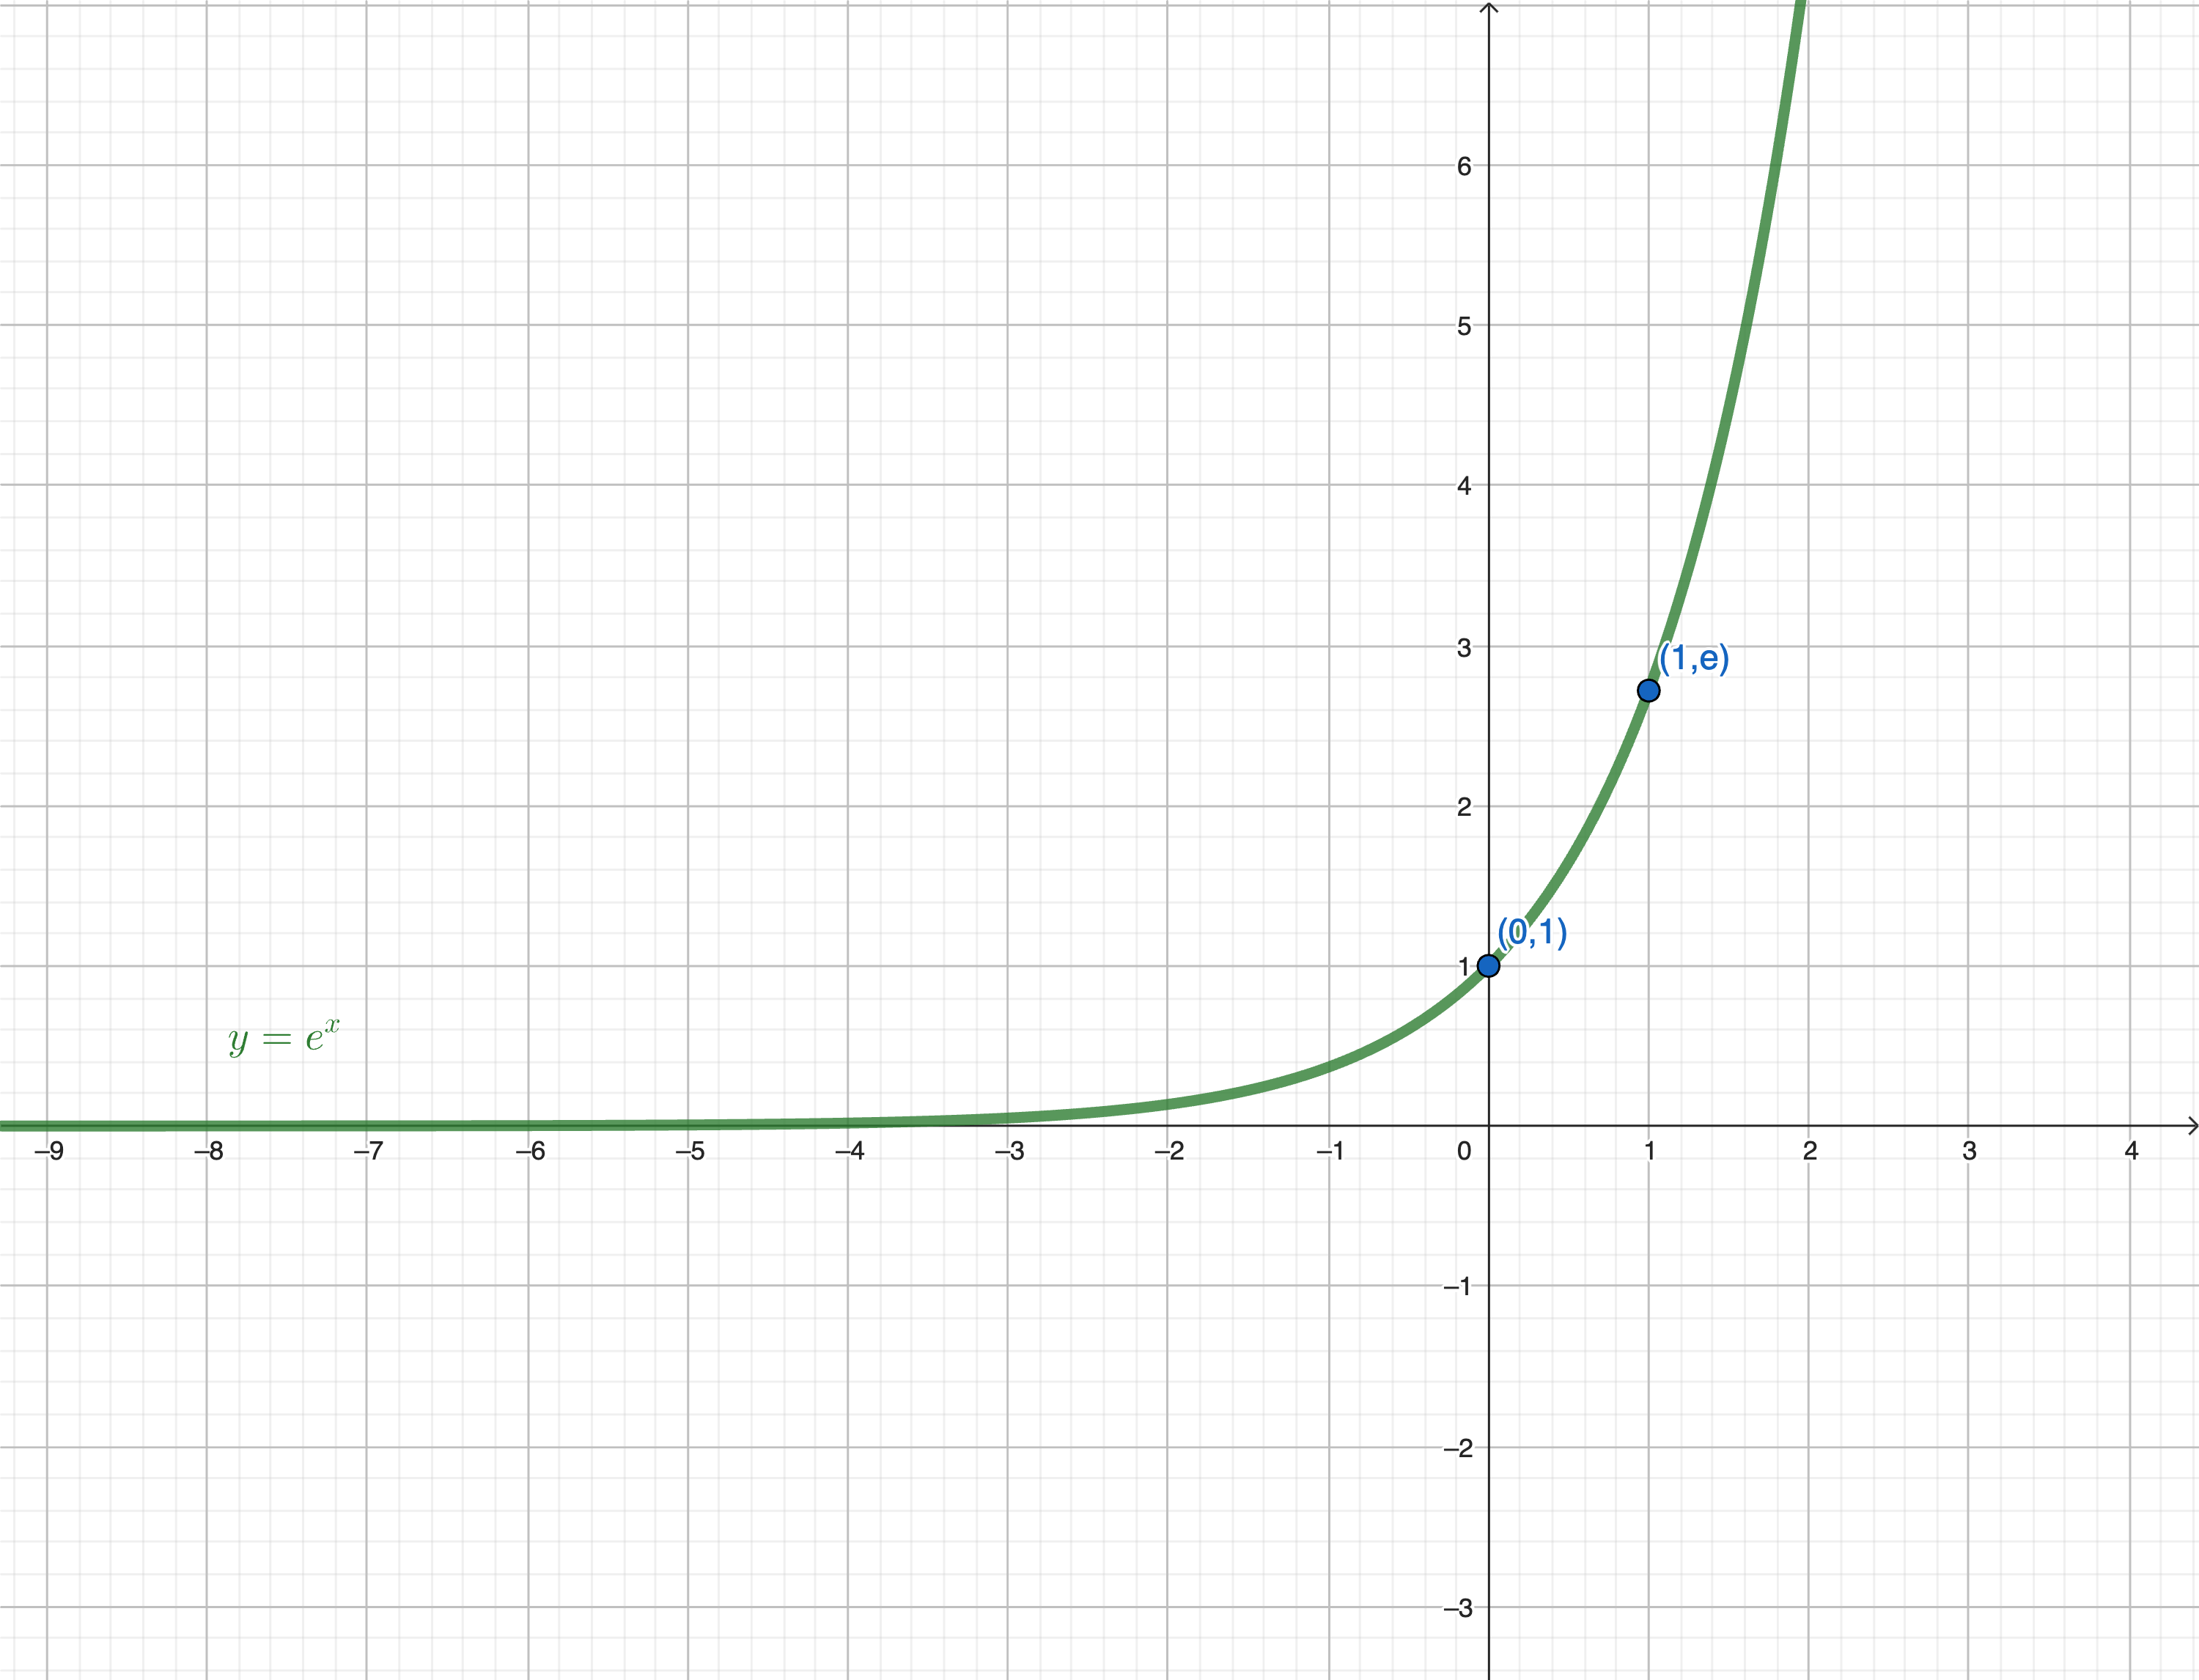
\includegraphics[width=.45\textwidth]{pics/exponencial.png}
\hfil
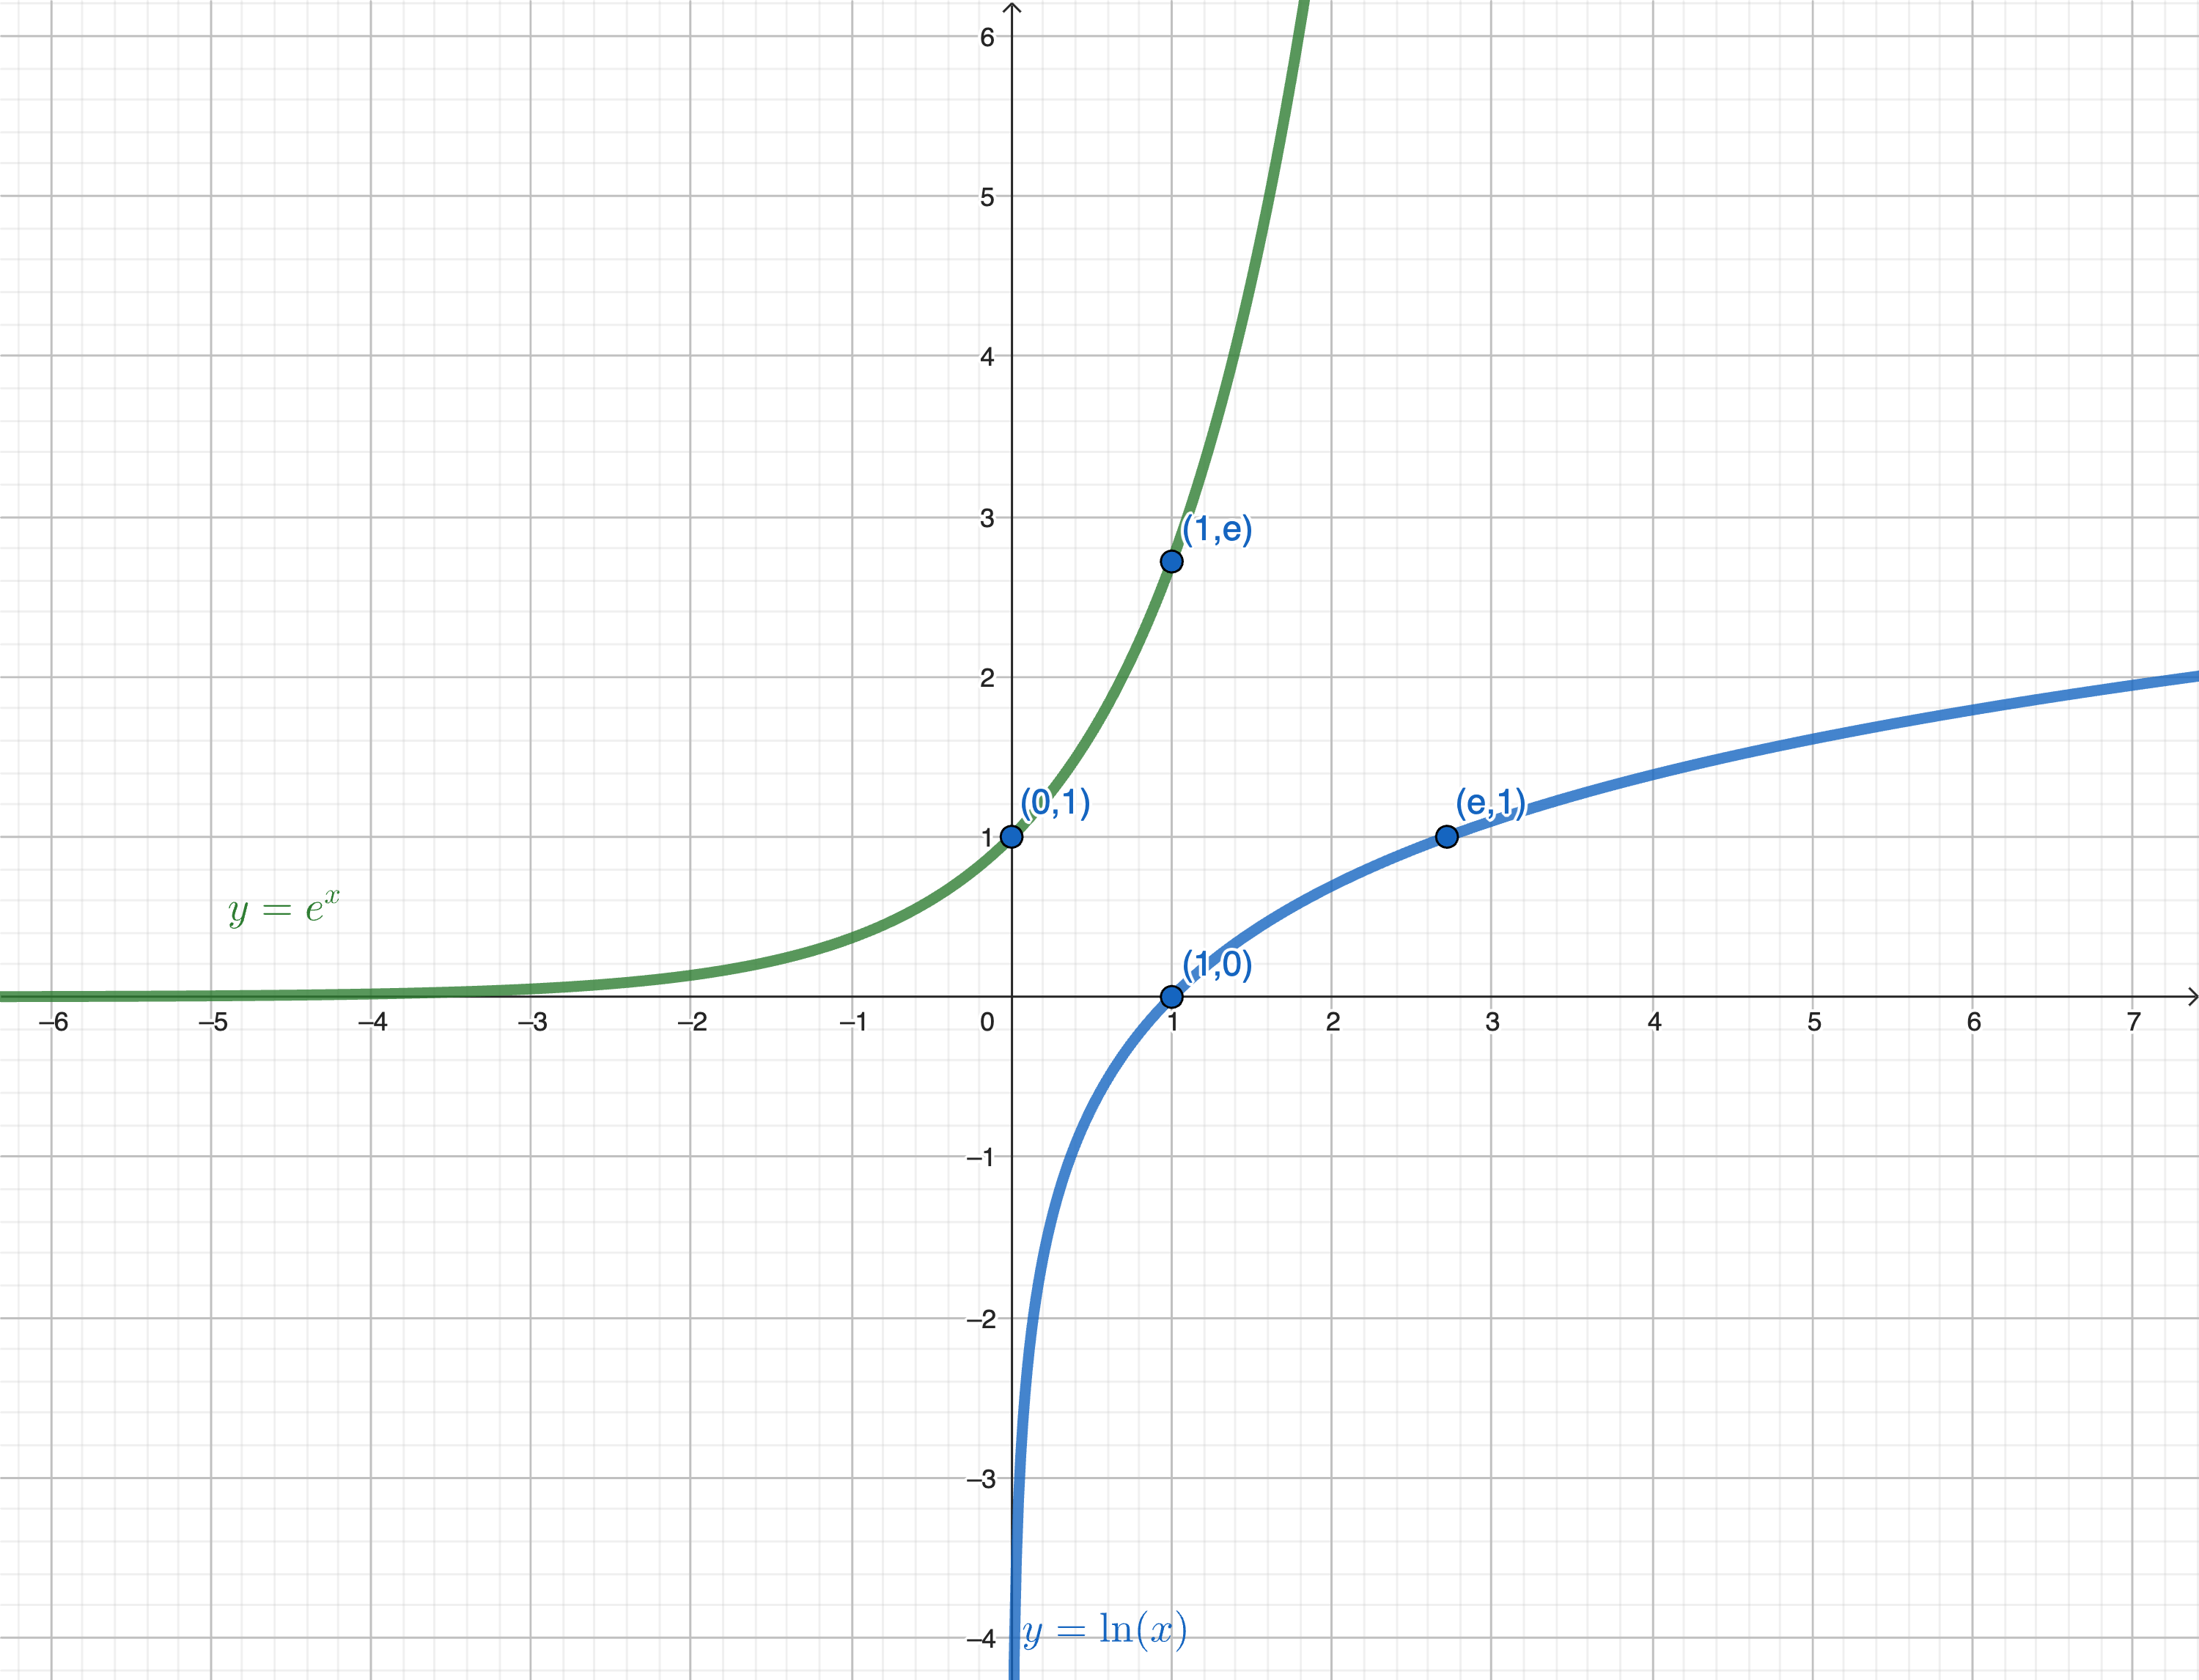
\includegraphics[width=.45\textwidth]{pics/exponencial-logaritmo.png}
}

Al ser $e^x$ biyectiva, tiene una función inversa, que es lo suficientemente importante como para recibir un nombre propio.

\begin{definition}
    Si $f:\R\to(0,+\infty)$ está dada por $f(x) = e^x$, entonces su función inversa se denomina \emph{función logaritmo} o \emph{función logaritmo natural} y se indica con $\ln : (0,+\infty) \to \R$. Para cada número $x > 0$ existe un único $y=\ln x\in\R$ que cumple:
    \[
    \ln x = y 
    \qquad\iff\qquad
    e^y = x.
    \]
    Dicho $y$ se llama \emph{logaritmo natural de $x$}.
\end{definition}

A partir de las propiedades enunciadas en el Teorema~\ref{T:exponencial propiedades} podemos deducir lo siguiente.

\begin{proposition}\label{P:logaritmo propiedades}
        \begin{enumerate}
        \item Si $x,y>0$, entonces $\ln (x\cdot y) = \ln(x) + \ln(y)$.
        \item Si $x > 0$ y $y\in\R$, entonces $\ln x^y = y \cdot \ln x$.
    \end{enumerate}
\end{proposition}

\begin{proof}
Ejercicio.
\end{proof}


De manera similar a como se hizo en el Teorema~\ref{P:exp biyectiva} se puede probar la siguiente proposición.

\begin{proposition}
    Si $a>0$, $a\neq 1$, la función $f:\R \to (0,+\infty)$ dada por $f(x) = a^x$ es biyectiva. Si $a>1$ $f$ es creciente y si $a<1$ $f$ es decreciente.
\end{proposition}

?`Por qué piensa el lector que no se estudia la función $a^x$ para $a=1$? ?`Y para $a<0$?

\begin{definition}
    Si $a>0$, $a\neq 1$, se define la función \emph{logaritmo en base $a$} como la inversa de $a^x$, es decir
    \[
    \log_a x = y \qquad\iff\qquad a^y = x.
    \]
    Es decir, el logaritmo en base $a$ de $x$ es la potencia a la que se debe elevar $a$ para obtener $x$.
\end{definition}

Para finalizar esta sección, demostramos la siguiente propiedad, realmente sorprendente.

\begin{proposition}
    Si $a>0$, entonces $\D \lim n (\sqrt[n]{a}-1) = \ln a$.
\end{proposition}

\begin{proof}
    Consideremos primero el caso $a\ge 1$ y sea $x=\ln a$, es decir, $e^x=a$, con $x\ge 0$.
    En primer lugar, recordemos que por el ejercicio~\ref{ej:eab} de la Sección~\ref{S:numero e}, tenemos que 
    \[
    \lim\big(1+\frac xn\big)^n = e^x.
    \]
    Veamos ahora que 
    \begin{align*}
        n (\sqrt[n]{a}-1) - \ln a &= n (\sqrt[n]{a}-1) - x 
        = n (\sqrt[n]{a}-1) - n\big( (1+\frac xn\big)^{n/n} - 1\big)
        \\
        &= n \left[ \sqrt[n]{a} - \sqrt[n]{(1+\frac xn\big)^n} \right].
    \end{align*}
    Esta última expresión es mayor o igual a cero, pues $(1+\frac xn)^{1/n}$ tiende \emph{crecientemente} a $e^x=a$.
    
    Si llamamos $\alpha = \sqrt[n]{a} $ y $\beta =  \sqrt[n]{(1+\frac xn\big)^n}$, tenemos que 
    \begin{align*}
    0\le \alpha - \beta 
    &= \frac{(\alpha-\beta)(\alpha^{n-1}+\alpha^{n-2}\beta + \dots +\alpha \beta^{n-2}+\beta^{n-1})}{\alpha^{n-1}+\alpha^{n-2}\beta + \dots +\alpha \beta^{n-2}+\beta^{n-1}}
    \\
    &= \frac{\alpha^n-\beta^n}{\alpha^{n-1}+\alpha^{n-2}\beta + \dots +\alpha \beta^{n-2}+\beta^{n-1}}.
    \end{align*}
    Como $x\ge 0$, $\beta \ge 1$, y como $a\ge 1$, también $\alpha \ge 1$.
    Por lo tanto, el denominador de la última expresión es mayor o igual a $n$, es decir, 
    \[
    \left[ \sqrt[n]{a} - \sqrt[n]{(1+\frac xn\big)^n} \right] 
    = \alpha - \beta \le \frac{\alpha^n - \beta^n) }n
    = \frac{ a - (1+\frac xn\big)^n}n
    \]
    Luego, 
    \[
    0\le n (\sqrt[n]{a}-1) - \ln a \le  a - (1+\frac xn\big)^n 
    = e^x - (1+\frac xn\big)^n\to 0, \quad\text{cuando $n\to\infty$}.
    \]
    Por el teorema del emparedado, $\lim n (\sqrt[n]{a}-1) - \ln a =0$, o lo que es lo mismo,
    $\lim n (\sqrt[n]{a}-1) = \ln a $.

    Si $0<a<1$, entonces $\ln a = - \ln \frac1a$ y $\frac1a>1$.
    Por lo que acabamos de ver
    \[ 
    \lim n \big(\sqrt[n]{\frac1a}-1\big) = \ln 1/a,
    \]
    pero 
    \[
    n \big(\sqrt[n]{\frac1a}-1\big) 
    = \frac{1}{\sqrt[n]{a}} n \big(1-\sqrt[n]{a}\big)
    = -\frac{1}{\sqrt[n]{a}} n \big(\sqrt[n]{a}-1\big).
    \]
    Esto implica que 
\[
n \big(\sqrt[n]{a}-1\big) = -\underbrace{\sqrt[n]{a}}_{\to 1} \underbrace{n \big(\sqrt[n]{\frac1a}-1\big) }_{\to \ln \frac1a} 
\to - 1 \cdot \ln\frac1a = \ln a.
\]
Hemos probado entonces el resultado que queríamos, tanto para $a\ge 1$ como para $0<a<1$. Es decir, para todo $a>0$.
    \end{proof}

\subsubsection*{Ejercicios de la sección~\getcurrentref{chapter}.\getcurrentref{section}}

\begin{enumerate}
\item Demostrar la Proposición~\ref{P:logaritmo propiedades}.

\item Demostrar las siguientes propiedades del logaritmo para $a>0$, $a\neq 1$:
\begin{enumerate}
    \item $\log_a (x\, y) = \log_a(x) + \log_a(y)$, para $x,y\in(0,+\infty)$.
    \item $\log_a (x^ y) = y \, \log_a(x)$, para $x\in(0,+\infty)$, $y\in\R$.
    \item $a^x = e^{x \ln a}$, para $x\in\R$.
    \item $\D\log_b x = \frac{\log_a(x)}{\log_a(b)}$, para $b>0$, $b\neq 1$ y $x>0$.
\end{enumerate}

\item Demostrar que $\log_a$ es creciente si $a>1$ y decreciente si $0<a<1$.

\item Sean $a,b > 0$. Probar que cualquiera sea $x \in \R$ se cumple que
\[
\text{a)}\quad (a\,b)^x = a^x\,b^x,
\qquad
\text{b)}\quad \Big(\frac ab\Big)^x = \frac{a^x}{b^x}.
\]
Ayuda: calcular $\ln(ab)^x$ y usar que $\ln$ es una función inyectiva.


\end{enumerate}


\section{Otras propiedades del límite}

Consideremos ahora una sucesión \sucan de términos positivos que tenga límite positivo $a$.
Podemos entonces considerar la sucesión que se obtiene tomando el logaritmo de cada término, es decir la sucesión $\big( \ln a_n \big)_\niN$ y también podemos considerar el logaritmo del límite $\ln a$. Lo que nos dice la siguiente proposición es que ambos resultados coinciden.

\begin{proposition}\label{P:logaritmo continuo}
    Sea \sucan una sucesión de términos positivos con límite también positivo:
    \[ 
    a = \lim a_n > 0.
    \]
    Entonces
    \[
    \lim \big(\ln a_n \big) = \ln a.
    \]
    O lo que es lo mismo
    \[
    \lim \big(\ln a_n \big) = \ln \big( \lim a_n \big).
    \]
\end{proposition}

\begin{proof}
    Sea $\epsilon>0$ arbitrario. Como $\lim a_n = a$ y $a\neq 0$, resulta $\lim \frac{a_n}a = 1$.
    Como $\epsilon>0$, $e^\epsilon > e^0=1$.
    Luego, existe $N_1\in\N$ tal que $\frac{a_n}{a} < e^\epsilon$, para todo $n\ge N_1$, y existe $N_2\in\N$ tal que $\frac{a_n}{a} > e^{-\epsilon}$, para todo $n\ge N_2$.
    Si definimos $N_0 = \max\{N_1,N_2\}$ entonces para $n\ge N_0$ se cumple que
    \[
    e^{-\epsilon} < \frac{a_n}a < e^\epsilon.
    \]
    Aplicando logaritmo, usando que el logaritmo es una función creciente, resulta
    \[
    \ln(e^{-\epsilon}) < \ln\big(\frac{a_n}a\big) < \ln(e^\epsilon),
    \qquad\text{para todo $n \ge N_0$},
    \]
    es decir,
    \[
    -\epsilon < \ln a_n - \ln a < \epsilon, \qquad\text{para todo $n \ge N_0$},
    \]
    que a su vez equivale a 
    \[
    |\ln a_n - \ln a| < \epsilon, \qquad\text{para todo $n \ge N_0$}.
    \]
    Hemos demostrado entonces que dado $\epsilon > 0$, existe $N_0\in\N$ tal que
    $|\ln a_n - \ln a| < \epsilon$, para todo $n \ge N_0$, o lo que es lo mismo, $\lim \ln a_n = \ln a$.
\end{proof}

La siguiente desigualdad será una herramienta útil en los resultados que siguen:

\begin{lemma}
    Sea $a > 1$. Entonces, para todo $x\in\R$ tenemos que
    \[
    \big| a^x - 1 \big| \le a^{|x|}-1.
    \]
\end{lemma}

\begin{proof}
Como $a>1$, la función $x\to a^x$ es creciente. Luego,
    si $x\ge 0$, se tiene que $a^x \ge a^0 = 1$ y por lo tanto
    \[
    \big| a^x - 1 \big| = a^x - 1 = a^{|x|} - 1,
    \]
    y la desigualdad deseada se cumple como igualdad.

    Veamos ahora qué ocurre cuando $x<0$. En este caso, $|x| = -x > 0$ y por lo tanto
    \begin{align*}
        \big| a^x - 1 \big| &= \big| 1 - a^x \big|
        = \big| 1 - \frac{1}{a^{-x}} \big|
        = \big| \frac{a^{-x} - 1}{a^{-x}} \big| 
        = \frac{1}{|a^{-x}|} |a^{-x}-1|
        \\
        &=  \frac{1}{a^{-x}} (a^{-x}-1)
        =  \frac{1}{a^{|x|}} (a^{|x|}-1)
        \le a^{|x|}-1.  \qedhere
    \end{align*}
\end{proof}

Ahora podemos demostrar que se puede tomar límite en una potencia:

\begin{lemma}\label{L:exp continua}
    Si $a>0$ y $\lim b_n = b$, entonces
    \[
    \lim a^{b_n} = a^b.
    \]
\end{lemma}

\begin{proof}
    La demostración de este lema hace uso del lema anterior. Supongamos primero que $a>1$. Luego
    \begin{align*}
        \big| a^{b_n} - a^b \big| 
        &= \big| a^{b_n-b+b} - a^b \big| 
        = \big| a^{b_n-b} a^b - a^b \big| 
        = \big| a^{b_n-b} - 1 \big| a^b
        \le \big( a^{|b_n-b|} - 1 \big) a^b.
    \end{align*}
    Sea ahora $k\in\N$ arbitrario. Como $\lim b_n = b$ existe $N_0\in\N$ tal que 
    \[
    |b_n-b|\le \frac1k,\qquad\text{para todo $n\ge N_0$}.
    \]
    Recordando la desigualdad de Bernoulli (Proposición~\ref{P:Bernoulli} con $h=a^{1/k}-1$ y $n=k$), tenemos que
    \[
    1 + k (a^{1/k}-1) \le \big(1 + (a^{1/k}-1)\big)^k = a,
    \]
    por lo que $\D a^{1/k}-1 \le \frac{a-1}k$.
    Luego
    \begin{align*}
        \big| a^{b_n} - a^b \big| 
        &\le \big( a^{|b_n-b|} - 1 \big) a^b
        \le  \big( a^{1/k} - 1 \big) a^b 
        \le \frac{a-1}k \, a^b.
    \end{align*}
    Sea ahora $\epsilon > 0$ y elijamos $k \in \N$ tal que 
    \[
    k > \frac{(a-1)\, a^b}{\epsilon}.
    \]
    Y sea $N_0\in\N$ que cumple lo anterior para ese $k$. Luego, para $n\ge N_0$ resulta
    \begin{align*}
        \big| a^{b_n} - a^b \big| 
        &< \frac{a-1}k \, a^b < \frac{a-1}{\frac{(a-1)\, a^b}{\epsilon}} \, a^b
        = \epsilon.
    \end{align*}    
    Hemos probado entonces que dado $\epsilon>0$, existe $N_0\in\N$ tal que
    \[
        \big| a^{b_n} - a^b \big| < \epsilon, \qquad\text{para todo $n\ge N_0$},
    \]
    es decir, $\lim a^{b_n} = a^b$. 

    Si $a=1$ el lema es trivial, pues $a^{b_n} = 1 = a^b$ para todo $n$.

    Si $0<a<1$, entonces $1/a>1$ y por lo que recién demostramos
    $\lim\big( 1/a \big)^{b_n} = 1/a$.
    Finalmente, por la Proposición~\ref{P:suc-lim-cociente}
    \[
    \lim a^{b_n} = \lim \frac{1}{(1/a)^{b_n}} = \frac{1}{\lim (1/a)^{b_n}}
     = \frac{1}{(1/a)^b} = a^b. \qedhere
    \] 
\end{proof}

La afirmación de este último lema era un caso particular de la siguiente proposición, pero un paso intermedio necesario para demostrarla.

\begin{proposition}\label{P:potencias continuas}
    Sea \sucan una sucesión de términos positivos con límite $a>0$ y sea \sucbn una sucesión con límite $b$. Entonces
    \[
    \lim a_n^{b^n} = a^b.
    \]
\end{proposition}

\begin{proof}
    Recordemos que el logaritmo natural es la función inversa de la función exponencial, así, para cualquier $x>0$, resulta $x = e^{\ln x}$. Aplicando esto a $x=a_n^{b_n}$ obtenemos
    \[
    a_n^{b^n} = e^{\ln a_n^{b_n }} = e^{b_n \ln a_n}.
    \]
    Si ahora consideramos la sucesión $c_n = b_n \ln a_n$, vemos que $\lim c_n = b \ln a$.
    Luego, por el lema anterior, $\lim e^{b_n \ln a_n} = e^{b \ln a} $, que finalmente implica lo siguiente:
    \[
    \lim a_n^{b^n} = \lim e^{b_n \ln a_n} = e^{b \ln a} = a^b. \qedhere
    \]
\end{proof}

Por último, también se cumplen las siguientes proposiciones, cuya demostración queda como ejercicio.

\begin{proposition}
    Si $a_n>0$ para todo \niN y $\lim a_n = 0$, entonces $\lim \ln(a_n) = -\infty$.
\end{proposition}
\begin{proof}
    Ejercicio.
\end{proof}

\begin{proposition}
    Si $\lim a_n = +\infty$, entonces $\lim \ln(a_n) = +\infty$.
\end{proposition}

\begin{proof}
    Ejercicio.
\end{proof}

\subsubsection*{Ejercicios de la sección~\getcurrentref{chapter}.\getcurrentref{section}}

\begin{enumerate}
\item Hallar los límites de las sucesiones dadas por:
\begin{multicols}{2}
    \begin{enumerate}
    \item $\D a_n = \Big( \frac{2n^2+3n-1}{3n^2-6n+1} \Big)^{2n}$
    \item $\D a_n = \Big( \frac{3n+4}{2n+5} \Big)^{\sqrt{n+1}-\sqrt{n}}$
    \item $\D a_n = \Big( \frac{3n+4}{3n-5} \Big)^{n}$
    \item $\D a_n = \Big( \frac{3n+4}{3n-5} \Big)^{n^2}$
    \item $\D a_n = \Big( \frac{3n+4}{3n-5} \Big)^{\sqrt{n}}$
    \item $\D a_n = \frac{\ln n}n$
    \end{enumerate}
\end{multicols}

\item Probar $\lim a_n = +\infty$ y $\lim b_n = b > 0$, entonces $\lim a_n^{b_n} = +\infty$.

\item Probar que si $\lim a_n = a > 1$ y $\lim b_n = +\infty$,
entonces $\lim a_n^{b_n} = +\infty$.

\end{enumerate}


\section{Teorema de Bolzano-Weierstrass}

En esta sección vamos a demostrar un teorema del cual haremos uso repetido en el resto del curso. Comenzamos con una definición.

\begin{definition}
    Un encaje de intervalos es una sucesión de intervalos cerrados $I_n = [a_n,b_n]$, con $a_n\le b_n$ tal que 
    \[
    I_1 \supset I_2 \supset I_3 \dots,
    \]
    es decir
    \[
    a_1 \le a_2 \le a_3 \le \dots,
    \qquad
    b_1 \ge b_2 \ge b_3 \ge \dots.
    \]
    En otras palabras, la sucesión \sucan es creciente y la sucesión \sucbn es decreciente, y además, todo $b_k$ es cota superior de \sucan y todo $a_k$ es cota inferior de \sucbn. Esquemáticamente:
    \[
    a_1 \le a_2 \le a_3 \le \dots
    \le b_3 \le b_2 \le b_1.
    \]
\end{definition}

Llamaremos \emph{longitud} del intervalo $I_n = [a_n,b_n]$ al número $b_n-a_n$, y lo denotaremos con $|I_n|$. Es decir, $|I_n| = |[a_n,b_n]| = b_n-a_n$.

\begin{theorem}
    Sea $(I_n)_\niN$ un encaje de intervalos que satisface $\lim |I_n| = 0$. Entonces existe un único $x \in \R$ que pertenece a todos los intervalos. Es decir
    \[
    \bigcap_{n=1}^\infty I_n = \{ x \}.
    \]
\end{theorem}

\begin{proof}
    Sean $a_n$, $b_n$ los extremos del intervalo $I_n$, es decir, $I_n=[a_n,b_n]$.
    Observemos que por la definición de encaje de intervalor, \sucan es creciente y acotada, por lo que existe $x=\lim a_n$. Ahora, como \sucan es creciente, $x \ge a_n$ para todo \niN.
    Por otro lado, $a_k \le b_n$, para todo $k,n\in\N$ , por lo tanto, $x 
    = \lim_{k\to\infty} a_k \le b_n$ para todo \niN. Es decir, $a_n\le x \le b_n$, o lo que es lo mismo, $x\in [a_n,b_n]=I_n$, para todo \niN.

    Ahora veamos la unicidad. Si $x,x' \in I_n$, para todo \niN, entonces 
    \[
    |x-x'| \le b_n-a_n = |I_n| \to 0,
    \]
    por lo que $|x-x'|=0$ o lo que es lo mismo, $x=x'$.
\end{proof}

Como consecuencia de este teorema se obtiene el \emph{Teorema de Bolzano-Weierstrass}, para lo cual tenemos que definir el concepto de \emph{subsucesión}, que consiste en elegir algunos elementos de una sucesión dada. Informalmente, una subsucesión de la sucesión \sucan es una sucesión de la forma:
    \[
    a_{n_1}, a_{n_2}, a_{n_3}, \dots,
    \]
    con $n_1<n_2<n_3<\dots$.

En otras palabras, si $\big(n_k\big)_{k\in\N}$ es una sucesión estrictamente creciente de números naturales, entonces $\big(a_{n_k}\big)_{k\in\N}$ es una subsucesión de \sucan.

Si recordamos que la definición de sucesión \sucan es como una función $a:\N\to\R$ donde denotamos $a_n = a(n)$, podemos definir precisamente una subsucesión de la siguiente manera.

\begin{definition}
Sea $a:\N\to\R$ una sucesión, e indiquemos $a_n=a(n)$. Una \emph{subsucesión} de \sucan es la composición
\[
a \circ n : \N \to \R
\]
de $a$ con una función \emph{estrictamente creciente} $n:\N \to \N$. Indicaremos $n_k = n(k)$ y luego $a_{n_k} = a_{n(k)} = a(n(k)) = a\circ n(k)$.
\end{definition}

Dos ejemplos claros de subsucesiones de una sucesión \sucan son los que se obtienen tomando los elementos de la sucesión que tienen índice par, o impar. Así, dos subsucesiones de \sucan son:
\[
a_2, a_4, a_6, \dots,\qquad\text{y}\qquad
a_1, a_3, a_5, \dots.
\]
La primera subsucesión es la que corresponde a $n_k = 2k$, $k\in\N$, que se denota $\big(a_{2k}\big)_{k\in\N}$ y la segunda es la que corresponde a $n_k = 2k-1$, $k\in\N$, que se escribe $\big(a_{2k-1}\big)_{k\in\N}$.

Hemos visto que toda sucesión convergente es acotada. 
La recíproca de esta afirmación no es cierta, ya que una sucesión acotada puede no ser convergente, por ejemplo la que está dada por $a_n = (-1)^n$.
Pero hay algo que se puede afirmar acerca de la convergencia de las sucesiones acotadas, y es lo que se plantea en el siguiente Teorema.

\begin{theorem}[Teorema de Bolzano-Weierstrass]
\label{T:Bolzano-Weierstrass} 
    Toda sucesión acotada contiene una subsucesión convergente.
\end{theorem}

\begin{proof}
    La demostración de este teorema es interesante y constructiva, y se verá en las clases de Coloquio de demostraciones.
\end{proof}

\subsubsection*{Ejercicios de la sección~\getcurrentref{chapter}.\getcurrentref{section}}

\begin{enumerate}
\item Consideremos las sucesiones
\[
b_n = \frac{1^2+2^2 + \dots + (n-1)^2}{n^3},
\qquad
c_n = \frac{1^2+2^2 + \dots + n^2}{n^3},
\]
e $I_n = [b_n,c_n]$.  Probar que $\big( I_n \big)_\niN$ es un encaje de intervalos cuyas longitudes tienden a cero. Hallar la intersección de todos ellos.

\item \begin{enumerate}
    \item 
Dar un ejemplo de un encaje de intervalos tal que la intersección de todos ellos contenga más de un punto.
\item* Probar que la intersección de todos los intervalos cerrados de un encaje de intervalos $\left(I_n\right)_{\niN}$ cualquiera es un intervalo cerrado. Ayuda: llamar $a_n$ y $b_n$ a los extremos izquierdo y derecho de $I_n$, respectivamente y luego definir $a = \sup \{a_n:\niN\}$ y $b = \inf\{b_n:\niN\}$; finalmente probar que la intersección es $[a,b]$.

\item Dar un ejemplo de una sucesión $\left(I_n\right)_{\niN}$ de intervalos \emph{abiertos} tales que $I_{n+1}\subset I_n$, $\forall\niN$ y tal que $\bigcap_{n=1}^\infty = \emptyset.$
\end{enumerate}

\end{enumerate}


\section{Sucesiones de Cauchy}

Antes, antes de entrar en tema, probamos un resultado sobre sucesiones y subsucesiones.

\begin{proposition}\label{P:caracterizacionporsubsucesiones}
    Una sucesión \sucan es convergente con límite $a$ si y sólo si toda subsucesión de \sucan es convergente con el mismo límite $a$.
\end{proposition}

\begin{proof}
Supongamos primero que $\lim a_n = a$ y sea \subsucan una subsucesión de \sucan. Es decir, $\left(n_k\right)_{k\in\N}$ es una sucesión estrictamente creciente de números naturales.
Dado $\epsilon > 0$, existe $N_0\in\N$ tal que 
\[
|a_n - a| < \epsilon, \quad\text{para todo $n\ge N_0$}.
\]
Ahora bien, como $n_k$ es una sucesión estrictamente creciente de números naturales, resulta que $n_k \ge k$, para todo $k\in\N$. Luego, si $k \ge N_0$, resulta que $n_k \ge k \ge N_0$ y luego $\big|a_{n_k} - a \big| < \epsilon$. Hemos probado que dado $\epsilon>0$ existe $N_0\in\N$ tal que 
\[
|a_{n_k} - a| < \epsilon, \quad\text{para todo $k\ge N_0$}.
\]
Es decir, $\lim_{k\to\infty} a_{n_k} = a$.

Supongamos ahora que toda subsucesión de \sucan converge con límite $a$. Entonces consideramos la subsucesión correspondiente a $n_k = k$, $k\in\N$, que coincide con la sucesión original.
Luego, esta subsucesión tiene límite $a$ y por lo tanto la sucesión original tiene límite $a$.
\end{proof}

Esta proposición es muy útil para demostrar cuando una sucesión no converge.
Si consideramos la sucesión \sucan dada por $a_n = (-1)^n$, vemos que la subsucesión $a_{2n}$ es la sucesión constantemente 1, que tiende a 1, y la subsucesión $a_{2n-1}$ es constantemente $-1$. Por lo tanto hay dos subsucesiones con diferente límite, y la sucesión original no converge.

Para definir sucesión convergente, lo que hicimos fue escribir de manera precisa la idea de que los términos de la sucesión se vayan acercando a un cierto número. Ahora, escribiremos de manera precisa la idea siguiente: que los términos de la sucesión se vayan acercando entre sí. Lo haremos de la siguiente manera:

\begin{definition}
    Se dice que una sucesión \emph{es de Cauchy} si cumple la siguiente propiedad:
    \begin{quote}
        Dado $\epsilon > 0$, existe $N_0 \in\N$ tal que
        \[
        \text{si $n,m\in\N$, $n\ge N_0$, $m\ge N_0$} \quad\text{entonces}\quad
        \big| a_n - a_m \big| < \epsilon.
        \]
    \end{quote}
\end{definition}

Veremos a continuación que una sucesión converge, sí, solo si es de Cauchy.
Comenzamos probando que toda sucesión de Cauchy es acotada.

\begin{proposition}\label{P:Cauchy=>Acotada}
    Si \sucan es una sucesión de Cauchy, entonces es acotada.
\end{proposition}

\begin{proof}
    Sea \sucan una sucesión de Cauchy. Consideremos $\epsilon = 1$ en la definición de sucesión de Cauchy. Luego, existe $N_0$ tal que, si $n,m\ge N_0$, resulta $|a_n-a_m|<1.$
    En particular, $|a_n - a_{N_0}| < 1$, para todo $n\ge N_0$. Es decir
    \[
    -a_{N_0} + 1 < a_n < a_{N_0} + 1, \qquad \text{para todo $n\ge N_0$}. 
    \]
    De esta manera, vemos que está acotada la sucesión a partir de $N_0$. Lo que resta es acotar los primeros $N_0$ términos, pero son un número finito de términos.
    Más precisamente, consideramos
    \begin{align*}
        M &= \max\{a_1, a_2, \dots, a_{N_0-1}, a_{N_0}+1\}, 
        \\
        m &= \min\{a_1, a_2, \dots, a_{N_0-1}, -a_{N_0}+1\}, 
    \end{align*}
    y entonces resulta que
    \[
    m \le a_n \le M, \qquad \text{para todo \niN}.
    \]
    Por lo tanto, la sucesión es acotada.
\end{proof}

El segundo paso de la demostración consiste en probar que si una sucesión de Cauchy tiene una subsucesión convergente, entonces toda la sucesión converge.

\begin{proposition}\label{P:Cauchy+subsuc=>convergencia}
    Sea \sucan una sucesión de Cauchy, y supongamos que existe una subsucesión \subsucan tal que $\lim_{k\to\infty} a_{n_k} = a$.
    \mara{Entonces la sucesión converge a $a$.}
\end{proposition}

\begin{proof}
    Sea $\epsilon>0$, arbitrario. Como la sucesión \sucan es de Cauchy, existe $N_0\in\N$ tal que
    \[
    |a_n - a_n | < \frac\epsilon2,\qquad\text{para todo $n,m\ge N_0$}.
    \]
    Como la subsucesión \subsucan converge a $a$, existe $N_0'\in\N$ tal que 
    \[
    | a_{n_k} - a | < \frac\epsilon2,\qquad\text{para todo $k \ge N_0'$}.
    \]
    En particular, si $k_0 \ge \max\{N_0,N_0'\}$, $n_{k_0} \ge k_0 \ge \max\{N_0,N_0'\}$ y resulta, para $n\ge N_0$,
    \[
    |a_n - a| = |a_n - a_{n_{k_0}} + a_{n_{k_0}} - a|
    \le |a_n - a_{n_{k_0}}| + |a_{n_{k_0}} - a|
    < \frac\epsilon2 + \frac\epsilon2 = \epsilon,
    \]
    lo cual prueba la afirmación de la proposición.
\end{proof}

Ahora estamos en condiciones de probar el resultado anunciado.

\begin{theorem}\label{T:converge sii Cauchy}
    Una sucesión es convergente si y sólo si es de Cauchy.
\end{theorem}

\begin{proof}
    Supongamos primero que \sucan es convergente con límite $a$. Entonces, dado $\epsilon>0$ existe $N_0\in\N$ tal que, si $n\ge N_0$, resulta $|a_n-a|<\epsilon/2$.
    Luego, si $n,m\ge N_0$,
    \[
    |a_n - a_m| = |a_n - a + a - a_m| \le |a_n-a| + |a-a_m| 
    < \frac\epsilon2 + \frac\epsilon2 = \epsilon.
    \]
    Hemos demostrado entonces que la sucesión es de Cauchy.

    Supongamos ahora que la sucesión es de Cauchy. Entonces, por la Proposición~\ref{P:Cauchy=>Acotada} la sucesión resulta acotada y por el Teorema~\ref{T:Bolzano-Weierstrass} debe contener una subsucesión convergente.
    Finalmente, la Proposición~\ref{P:Cauchy+subsuc=>convergencia}, la sucesión resulta convergente.
\end{proof}

\subsubsection*{Ejercicios de la sección~\getcurrentref{chapter}.\getcurrentref{section}}

\begin{enumerate}
\item Demostrar que si $\left(n_k\right)_{k\in\N}$ es una sucesión estrictamente creciente de números naturales, entonces $n_k \ge k$, para todo $k\in\N$.
\item * Probar que una sucesión es de Cauchy si y sólo si dado $\epsilon>0$ existe $N_0\in\N$ tal que, para $n\ge N_0$ se cumple que
\[
|a_{n+p} - a_n| < \epsilon,\quad \text{cualquiera sea $p\in\N$}.
\]

\item Probar que si una sucesión es de Cauchy, entonces, cualquiera sea $p\in\N$ se cumple que
$\D\lim_{n\to\infty} (a_{n+p}-a_n) = 0$.

\item Mostrar que la recíproca del ejercicio anterior no es cierta. Ayuda. Considerar la sucesión dada por $a_n = \ln n$, ?`Cuál es $\lim a_n$? ?`Cuál es $\D\lim_{n\to\infty} (a_{n+p}-a_n)$? 

\item Demostrar que la sucesión dada por $a_n = (-1)^n+\frac1n$ no es convergente.

\item Encontrar tres ejemplos de sucesiones acotadas que no sean convergentes.


\end{enumerate}

\section{Ejercicios del capítulo~\getcurrentref{chapter}}
\begin{enumerate}
\input{ejercicios-ch-2-s-01}
\item Probar que la sucesión \emph{constante} $a_n=a$ para todo $n\in\N$, tiene límite $a$.

\item Probar que si $\lim a_n = a$, entonces $\lim |a_n| = |a|$ (ayuda, usar la desigualdad triangular del ejercicio~\ref{ej:triangular resta} del Capítulo~\ref{Cap:Reales}).

\item Probar las siguientes afirmaciones:

\begin{multicols}{2}
    \begin{enumerate}
        \item $\D \lim \frac1{\sqrt{n}} = 0 $
        \item $\D \lim \frac{1}{\sqrt{n+1}+\sqrt{n}} = 0 $
        \item $\D \lim \frac{(-1)^n}{3n^2-4n} = 0 $
        \item $\D \lim \frac{(-1)^{n-1}}{2-n^2} = 0 $
        \item $\D \lim \frac{n}{n+1} = 1 $
        \item $\D \lim \frac{3n}{4n+2} = \frac34 $
        \item $\D \lim \frac{2n+3}{n^2-2n-3} = 0 $
        \item $\D \lim \frac{-3n+1}{4n^2-3n+4} = 0 $
        \item $\D \lim \frac{3n^2+2n-2}{n^2+1} = 3 $
        \item $\D \lim \frac{2n^2-3n+1}{3n^2+2n-1} = \frac23 $
        \item $\D \lim \frac{n^2+n+1000}{3n^2-14n-7} = \frac13 $
        % \item $\D \lim \frac{n}{n^{3/2}+1} = 0 $
        % \item $\D \lim \frac{n^{2/3}+100}{n^{3/4}+4} = 0 $
        % \item $\D \lim \frac{3n^{2/3}+n^{4/5}+2n^{5/2}}{n^3+n^{2/3}+5n} = 0 $
        % \item $\D \lim \frac{2n^{3/4}+\sqrt n}{n^{3/4}} = 2 $
        % \item $\D \lim \frac{n^2-3n^{7/2}+20}{n^{7/2}-6n^3+3n^2-2n} = -3$
    \end{enumerate}
\end{multicols}

\item Probar que $\D \lim \big( \sqrt{n+1} - \sqrt{n}\big) = 0$.
(Sugerencia: multiplicar y dividir por \emph{el conjugado} $\sqrt{n+1} + \sqrt{n}$)

\item Sea $\big( a_n \big)_{n\in\N}$ una sucesión convergente con límite $\ell$. Probar que si $\big(b_n \big)_{n\in\N}$ está definida por 
\[
b_n = a_{n+1}, \qquad \text{o sea $b_1=a_2$, $b_2=a_3$, $b_3=a_4$, \dots},
\]
entonces $\D\lim b_n = \ell$.

\item Sea $\big( a_n \big)_{n\in\N}$ una sucesión convergente con límite $\ell$, y sea $p\in\N$.
Probar que si $\big(b_n \big)_{n\in\N}$ está definida por 
\[
b_n = a_{n+p}, \qquad \text{o sea $b_1=a_{p+1}$, $b_2=a_{p+2}$, $b_3=a_{p+3}$, \dots},
\]
entonces $\D\lim b_n = \ell$.

\item Sea $\big( a_n \big)_{n\in\N}$ una sucesión convergente con límite $\ell$, y sea $p\in\N$.
Probar que si $\big(b_n \big)_{n\in\N}$ está definida por 
\[
\begin{cases}
    b_1 &= \text{cualquier cosa},\\
b_2 &= \text{cualquier cosa},\\
 &\vdots\\
b_p &= \text{cualquier cosa},
\end{cases}
\qquad\qquad \text{y }\quad b_k = a_k, \ \text{ para } \ k>p,
\]
entonces $\D\lim b_n = \ell$.

\item Probar que si \sucan es una sucesión convergente y $c$ es un número real cualquiera, entonces $\lim (c \, a_n) = c\, \lim a_n$.

\item Probar que si \sucan es convergente y $k$ es un número \emph{natural} cualquiera, entonces $\lim a_n^k = \left(\lim a_n\right)^k$. (Ayuda: razonar por inducción sobre $k$ y usar la Proposición~\ref{P:suc-lim-prod})

\item Determinar cuáles de las siguientes afirmaciones son verdaderas y cuáles no (en caso afirmativo, dar una demostración, en caso negativo, un contraejemplo).
\begin{enumerate}
    \item Si $(a_n+b_n)_\niN$ es convergente, entonces \sucan y \sucbn son convergentes.
    \item Si $(a_n+b_n)_\niN$ es convergente y $\sucan$ es convergente, entonces \sucbn es convergente.
    \item Si $(a_n\cdot b_n)_\niN$ es convergente, entonces \sucan y \sucbn son convergentes.
    \item Si $(a_n\cdot b_n)_\niN$ es convergente y \sucan es convergente, entonces \sucbn es convergente.
    \item Si $(a_n\cdot b_n)_\niN$ es convergente y \sucan es convergente con límite distinto de cero, entonces \sucbn es convergente.
    \item Si $(a_n^2)_\niN$ es convergente, entonces \sucan es convergente.
    \item Si \sucan es convergente con límite cero y \sucbn es acotada, entonces $(a_n\cdot b_n)_\niN$ es convergente con límite cero.
\end{enumerate}

\item Calcular los siguientes límites:

\begin{multicols}{2}
    \begin{enumerate}
        \item $\D \lim \frac{3n^3+4n^2-6}{7+8n+9n^3} $
        \item $\D \lim \frac{1-2n+3n^2}{4+5n-6n^2} $
        \item $\D \lim \frac{1-2n+3n^2}{4+5n-6n^2+n^3} $
        \item $\D \lim \frac{1}{2 n^{3/2}} $
        \item $\D \lim \frac{1000 + 10 n - 2 n^{3/2}}{10 n^{3/2}} $
        \item $\D \lim \frac{1000 + 10 n - 2 n^{3/2}}{10 n^{3/2}-n^2} $

        \item $\D \lim \frac{n}{n^{3/2}+1} = 0 $
        \item $\D \lim \frac{n^{2/3}+100}{n^{3/4}+4} = 0 $
        \item $\D \lim \frac{3n^{2/3}+n^{4/5}+2n^{5/2}}{n^3+n^{2/3}+5n} = 0 $
        \item $\D \lim \frac{2n^{3/4}+\sqrt n}{n^{3/4}} = 2 $
        \item $\D \lim \frac{n^2-3n^{7/2}+20}{n^{7/2}-6n^3+3n^2-2n} = -3$
\end{enumerate}
\end{multicols}


    \item Calcular los siguientes límites:

    \begin{multicols}{2}
        \begin{enumerate}
            \item $\D \lim \frac{3n^4+4n^2-6}{7+8n+9n^3} $
            \item $\D \lim \frac{1-2n+3n^3}{4+5n-6n^2} $
            \item $\D \lim \frac{1-2n+3n^2}{4+5n-6n^2+n^3} $
            \item $\D \lim \frac{n^{3/2}}{10n+1} $
            \item $\D \lim \frac{1000 + 10 n - 2 n^{5/2}}{10 n^{3/2}} $
            \item $\D \lim \frac{1000 + 10 n - 2 n^{3/2}+n^2}{10 n^{3/2}-n^2} $
        \end{enumerate}
    \end{multicols}
    
\item Demostrar que si $r>0$ y \sucan es una sucesión tal que $|a_n| > r$, para todo \niN y \sucbn es una sucesión tal que $b_n\neq 0$ para todo $n$ y $\lim b_n = 0$, entonces
\[ \lim \frac{a_n}{b_n} = \infty. \]
Esto daría la regla de cálculo $\D\frac{a}{0} = \infty$ si $a\neq 0$.

\item Probar las siguientes afirmaciones
\begin{enumerate}
    \item Si \sucan es acotada y $\lim b_n = +\infty$, entonces $\lim\big(a_n+b_n) = +\infty$.
    \item Si \sucan es acotada y $\lim b_n = -\infty$, entonces $\lim\big(a_n+b_n) = -\infty$.
    \item Si $\lim a_n = +\infty$ y $\lim b_n = +\infty$, entonces $\lim\big(a_n+b_n) = +\infty$.
    \item Si $\lim a_n = -\infty$ y $\lim b_n = -\infty$, entonces $\lim\big(a_n+b_n) = -\infty$.
    \item Si $\lim a_n = +\infty$ y $\lim b_n = -\infty$, entonces $\lim\big(a_n\cdot b_n) = -\infty$.
\end{enumerate}

\item Mostrar, dando un contraejemplo en cada caso, que las siguientes afirmaciones son falsas.
\begin{enumerate}
    \item Si $\lim a_n = \infty$ y $\lim b_n = \infty$, entonces $\lim\big(a_n + b_n) = \infty$.
    \item Si $\lim a_n = a$ y $\lim b_n = \infty$, entonces $\lim\big(a_n \cdot b_n) = \infty$.
\end{enumerate}

\item Probar las siguientes afirmaciones:
\begin{enumerate}
    \item Si $\lim b_n = +\infty$ y $a_n \ge b_n$ para todo \niN, entonces $\lim a_n = +\infty$.
    \item Si $\lim b_n = -\infty$ y $a_n \le b_n$ para todo \niN, entonces $\lim a_n = -\infty$.
    \item Si $\lim a_n = a > 0$ y $\lim b_n = +\infty$, entonces $\lim\big(a_n\cdot b_n\big) = +\infty$.
    \item Si $\lim a_n = a < 0$ y $\lim b_n = +\infty$, entonces $\lim\big(a_n\cdot b_n\big) = -\infty$.
\end{enumerate}

\item Sean $f$ y $g$ funciones polinómicas de grados $h$ y $k$ respectivamente. Para cada natural $n$ están definidos $f(n)$ y $g(n)$. Probar
\[
\textbf{(a)}\quad \lim\frac{f(n)}{g(n)} = 0, \ \text{si $h<k$},
\qquad
\textbf{(b)}\quad \lim\frac{f(n)}{g(n)} = \infty, \ \text{si $h>k$}.
\]
?`Cuánto vale $\D \lim\frac{f(n)}{g(n)}$ si $h=k$?



\item Sea \sucan una sucesión tal que se cumple lo siguiente:
\begin{quote}
Existen $r,R$ positivos tales que $r < a_n < R$, para todo $n\in\N$.
\end{quote}
Demostrar que entonces $\lim \sqrt[n]{a_n} = 1$. 

\item Sea \sucan una sucesión convergente de términos positivos tal que:
\[
\lim a_n > 0.
\]
Demostrar que entonces $\lim \sqrt[n]{a_n} = 1$. 

\item Dar un ejemplo de una sucesión \sucan acotada y de términos positivos para la cual no sea cierto que $\lim \sqrt[n]{a_n} = 1$. 

\item Probar las siguientes afirmaciones.
\begin{enumerate}
    \item $\lim  \sqrt[n]{n^2} = 1$.
    \item $\lim  \sqrt[n]{n^3} = 1$.
    \item Si $k\in\N$, entonces $\lim \sqrt[n]{n^k} = 1$.
\end{enumerate}

\item Probar las siguientes afirmaciones.
\begin{enumerate}
    \item $\lim \sqrt[n]{n^2+n} = 1$.
    \item $\lim \sqrt[n]{n^2-n} = 1$.
    \item $\lim \sqrt[n]{3n^3+2n^2+2n+1} = 1$.
    \item $\lim \sqrt[n]{3n^3-4n^2+6n-3} = 1$.
\end{enumerate}

\item Calcular
\begin{enumerate}
    \item $\lim \sqrt[n]{3^n+2}$
    \item $\lim \sqrt[n]{3^n-2}$
    \item $\lim \sqrt[n]{(\frac12)^n+3}$
    \item $\lim \sqrt[n]{3^n+2^n}$
    \item $\lim \sqrt[n]{a^n+b^n}$, si $0 < a < b$.
\end{enumerate}

\item Sea \sucan una sucesión convergente con límite $a$.
Probar que
\begin{enumerate}
    \item $\lim a_n^n = +\infty$, si $a>1$.
    \item $\lim a_n^n = \infty$, si $a<-1$.
    \item $\lim a_n^n = 0$, si $|a|<1$.
\end{enumerate}
    \item Para las siguientes sucesiones, decir cuáles son crecientes, cuáles estrictamente crecientes, cuáles decrecientes, cuáles estrictamente decrecientes, y cuáles acotadas:
    \begin{multicols}{2}
        \begin{enumerate}
        \item $\D a_n = \frac{n}{n+1}$
        \mara{\item $\D b_n = \frac{n^2}{n+1}$}
        \item $\D c_n = \frac{n!}{n^n}$
        \item $\D d_n = \frac{1}{\sqrt{n+1}-\sqrt{n}}$
        \item $\D e_n = \frac{1}{n+1} + \frac{1}{n+2} + \dots + \frac{1}{2n}$
        \mara{\item $\D f_n = \frac{2^n-1}{2^n} $}
    \end{enumerate}
    \end{multicols}
\item Sea \sucan una sucesión decreciente. Demostrar que la sucesión $(-a_n)_{\niN}$ es creciente.


\item Probar que las siguientes sucesiones son convergentes, y calcular su límite:
    \begin{enumerate}
        \item $a_1 = \sqrt3$, $\D a_{n+1} = \sqrt{3+a_n}$, \niN.
        \item $b_1 = \sqrt5$, $\D b_{n+1} = \sqrt{5+b_n}$, \niN.
        \item \mara{$c_1 = 1$, $\D c_{n+1} = 1 + \sqrt{c_n}$, \niN.}
    \end{enumerate}


\item Hallar los límites de las sucesiones dadas por:
\label{ej:numero e} 

\begin{multicols}{2}
    \begin{enumerate}
    \item $\D a_n = \Big( 1-\frac1n \Big)^{n}$
    \item $\D a_n = \Big( 1-\frac1{n^ 2} \Big)^{n}$
    \item $\D a_n = \Big( \frac{2n+1}{2n+3} \Big)^{3n-2}$
    \item $\D a_n =  \frac{n}{\sqrt[n]{n!}} $
    \item $\D a_n = \Big( 1+\frac1n \Big)^{5}$
    \item $\D a_n = \Big( 1+\frac15 \Big)^{n}$
    \item $\D a_n = \frac{n}{e^ n}$
    \item $\D a_n = \Big( 1-\frac{1}{n}  \Big)^{n^2}$
    \item $\D a_n = \Big( 1+\frac1{2n} \Big)^{4n+1}$
    \item $\D a_n = \Big( \frac{3n
+4}{3n+2} \Big)^{2n-1}$
    \item\label{ej:eab}  $\D a_n = \Big( 1+\frac an \Big)^{b\,n}$
\end{enumerate}
\end{multicols}


\item Demostrar la Proposición~\ref{P:logaritmo propiedades}.

\item Demostrar las siguientes propiedades del logaritmo para $a>0$, $a\neq 1$:
\begin{enumerate}
    \item $\log_a (x\, y) = \log_a(x) + \log_a(y)$, para $x,y\in(0,+\infty)$.
    \item $\log_a (x^ y) = y \, \log_a(x)$, para $x\in(0,+\infty)$, $y\in\R$.
    \item $a^x = e^{x \ln a}$, para $x\in\R$.
    \item $\D\log_b x = \frac{\log_a(x)}{\log_a(b)}$, para $b>0$, $b\neq 1$ y $x>0$.
\end{enumerate}

\item Demostrar que $\log_a$ es creciente si $a>1$ y decreciente si $0<a<1$.

\item Sean $a,b > 0$. Probar que cualquiera sea $x \in \R$ se cumple que
\[
\text{a)}\quad (a\,b)^x = a^x\,b^x,
\qquad
\text{b)}\quad \Big(\frac ab\Big)^x = \frac{a^x}{b^x}.
\]
Ayuda: calcular $\ln(ab)^x$ y usar que $\ln$ es una función inyectiva.


\item Hallar los límites de las sucesiones dadas por:
\begin{multicols}{2}
    \begin{enumerate}
    \item $\D a_n = \Big( \frac{2n^2+3n-1}{3n^2-6n+1} \Big)^{2n}$
    \item $\D a_n = \Big( \frac{3n+4}{2n+5} \Big)^{\sqrt{n+1}-\sqrt{n}}$
    \item $\D a_n = \Big( \frac{3n+4}{3n-5} \Big)^{n}$
    \item $\D a_n = \Big( \frac{3n+4}{3n-5} \Big)^{n^2}$
    \item $\D a_n = \Big( \frac{3n+4}{3n-5} \Big)^{\sqrt{n}}$
    \item $\D a_n = \frac{\ln n}n$
    \end{enumerate}
\end{multicols}

\item Probar $\lim a_n = +\infty$ y $\lim b_n = b > 0$, entonces $\lim a_n^{b_n} = +\infty$.

\item Probar que si $\lim a_n = a > 1$ y $\lim b_n = +\infty$,
entonces $\lim a_n^{b_n} = +\infty$.

\item Consideremos las sucesiones
\[
b_n = \frac{1^2+2^2 + \dots + (n-1)^2}{n^3},
\qquad
c_n = \frac{1^2+2^2 + \dots + n^2}{n^3},
\]
e $I_n = [b_n,c_n]$.  Probar que $\big( I_n \big)_\niN$ es un encaje de intervalos cuyas longitudes tienden a cero. Hallar la intersección de todos ellos.

\item \begin{enumerate}
    \item 
Dar un ejemplo de un encaje de intervalos tal que la intersección de todos ellos contenga más de un punto.
\item* Probar que la intersección de todos los intervalos cerrados de un encaje de intervalos $\left(I_n\right)_{\niN}$ cualquiera es un intervalo cerrado. Ayuda: llamar $a_n$ y $b_n$ a los extremos izquierdo y derecho de $I_n$, respectivamente y luego definir $a = \sup \{a_n:\niN\}$ y $b = \inf\{b_n:\niN\}$; finalmente probar que la intersección es $[a,b]$.

\item Dar un ejemplo de una sucesión $\left(I_n\right)_{\niN}$ de intervalos \emph{abiertos} tales que $I_{n+1}\subset I_n$, $\forall\niN$ y tal que $\bigcap_{n=1}^\infty = \emptyset.$
\end{enumerate}

\item Demostrar que si $\left(n_k\right)_{k\in\N}$ es una sucesión estrictamente creciente de números naturales, entonces $n_k \ge k$, para todo $k\in\N$.
\item * Probar que una sucesión es de Cauchy si y sólo si dado $\epsilon>0$ existe $N_0\in\N$ tal que, para $n\ge N_0$ se cumple que
\[
|a_{n+p} - a_n| < \epsilon,\quad \text{cualquiera sea $p\in\N$}.
\]

\item Probar que si una sucesión es de Cauchy, entonces, cualquiera sea $p\in\N$ se cumple que
$\D\lim_{n\to\infty} (a_{n+p}-a_n) = 0$.

\item Mostrar que la recíproca del ejercicio anterior no es cierta. Ayuda. Considerar la sucesión dada por $a_n = \ln n$, ?`Cuál es $\lim a_n$? ?`Cuál es $\D\lim_{n\to\infty} (a_{n+p}-a_n)$? 

\item Demostrar que la sucesión dada por $a_n = (-1)^n+\frac1n$ no es convergente.

\item Encontrar tres ejemplos de sucesiones acotadas que no sean convergentes.


\end{enumerate}



\chapter{Series}

\section{Definición de serie}

Consideremos una sucesión cualquiera \sucan. Para cada \niN sabemos lo que significa la suma de los $n$ primeros términos de la sucesión, que indicamos
\[
\sum_{k=1}^n a_k = a_1+a_2+\dots+a_n.
\]
En este capítulo queremos darle sentido, si es posible, a la definición de suma de \emph{todos} los términos de la sucesión, que indicaremos
\[
\serieak = a_1+a_2 +a_3+\cdots.
\]

En busca de esa definición, consideremos las siguientes \emph{sumas parciales}
\begin{align*}
    S_1 &= a_1 \\
    S_2 &= a_1 + a_2 \\
    S_3 &= a_1 + a_2 + a_3\\
    &\vdots \\
    S_n &= a_1 + a_2 + a_3 + \dots + a_n \\
    &\vdots 
\end{align*}
Si estuviera definido \serieak sería razonable que los valores $S_n$ se acerquen a ese valor. Pero eso es lo mismo que pensar que la sucesión $\left(S_n\right)_\niN$ tenga límite, lo que en general no ocurre.

Por ejemplo, consideremos la sucesión dada por $a_n = (-1)^{n+1}$.
Para esta sucesión, tenemos
\begin{align*}
    S_1 &= a_1 = 1\\
    S_2 &= a_1 + a_2 = 1 + (-1) = 0\\
    S_3 &= a_1 + a_2 + a_3 = 1 + (-1) + 1 = 1\\
    &\vdots \\
    S_n &= a_1 + a_2 + a_3 + \dots + a_n = \begin{cases} 1, &\text{si $n$ es impar,}\\
    0, &\text{si $n$ es par}. 
    \end{cases}
    \\
    &\vdots 
\end{align*}
La sucesión de sumas parciales es
\[ 
1,\,0,\,1,\,0,\,\dots, 
\]
que claramente no es convergente.
Luego, no parece posible dar una definición de \serieak \emph{para cualquier} sucesión \sucan. 
Esto nos lleva a la siguiente definición.

\begin{definition}\label{D:sumaserie}
Para una sucesión \sucan definimos la sucesión de sumas parciales $\left(S_n\right)_\niN$ de la siguiente manera:
\[
S_n = \sum_{k=1}^n a_k, \qquad \niN.
\]
Si la sucesión $\left(S_n\right)_\niN$ es convergente, decimos que el límite de esa sucesión es la suma de los $a_k$ para $k=1$ hasta $\infty$: 
\[
\sum_{k=1}^\infty a_k = \lim S_n.
\]
O sea $\D \sum_{k=1}^\infty a_k = \lim_{n\to\infty} \Big(\sum_{k=1}^n a_k\Big)$.
\end{definition}

Brevemente, entonces, la suma de infinitos números reales es el límite de la sumas parciales, si dicho límite existe. Pero exista o no ese límite, vamos a encontrar de importancia el estudio de la sucesiones de sumas parciales correspondientes a una sucesión dada \sucan.

La expresión \emph{sucesión de sumas parciales correspondientes a una sucesión} \sucan es un poco larga como para estar usándola continuamente (y debemos hacerlo). Esto ha originado una abreviatura para esa expresión bastante singular: en lugar de decir, \emph{la sucesión de sumas parciales correspondiente a la sucesión \sucan} se dice \emph{la serie \seriean}.

De esta manera, aunque no exista \serieak (en el sentido de la Definición~\ref{D:sumaserie}), siempre existe la \emph{serie \serieak}. Por ejemplo, no existe $\sum_{k=1}^\infty (-1)^{k+1}$, pero sí existe \emph{la serie $\sum_{k=1}^\infty (-1)^{k+1}$}: es la sucesión $1$, $0$, $1$, $0$, \dots.

Más aún, aunque exista \seriean, no es lo mismo que \emph{la serie \seriean}, pues \seriean es un número, el límite de una sucesión, mientras que \emph{la serie \seriean} es dicha sucesión.

De acuerdo a lo anterior, está claro qué quiere decir que una serie sea convergente: como la serie por definición es una sucesión (la de las sumas parciales), entonces eso querrá decir que dicha sucesión es convergente.

El núcleo de este capítulo estará en la determinación de criterios que nos permitan decidir si una serie es convergente o no.

Empezamos probando lo siguiente:

\begin{proposition}\label{P:serie convergente termino tiende a cero}
    Si la serie \seriean converge, entonces $\lim a_n = 0$.
\end{proposition}

\begin{proof}
    Que la serie \seriean sea convergente quiere decir que la sucesión \sucSn de sumas parciales converge, digamos a un límite $\ell\in\R$. Luego,
    \[
    \lim (S_{n+1}-S_n) = \lim S_{n+1} - \lim S_n = \ell - \ell = 0.
    \]
    Pero $S_{n+1} - S_n = \sum_{k=1}^{n+1} a_k - \sum_{k=1}^n a_k = a_{n+1}$, es decir, $\lim a_{n+1} = 0$, o lo que es lo mismo $\lim a_n = 0$.
\end{proof}

Desafortunadamente, la recíproca de esta Proposición~\ref{P:serie convergente termino tiende a cero} no es cierta: \emph{no} es cierto que si $a_n \to 0$ entonces la serie \seriean converge; veremos en la sección siguiente un ejemplo de esto.

Ya estamos en condiciones de examinar un ejemplo muy importante, la llamada \emph{serie geométrica de razón $r$}. Esta es la serie
\[
\sum_{k=1}^\infty r^{k-1}, \qquad \text{también indicada }
\sum_{k=0}^\infty r^k,
\]
definida para $r\in\R$ arbitrario. Veamos cuál es su comportamiento según cuál sea el valor de $r$.

Recordemos que, para $r\neq 1$, tenemos una fórmula para la suma parcial 
\[ 
S_n = 1+r+r^2 + \dots + r^{n-1} = \frac{r^n-1}{r-1}
\]
(si no recuerda esta fórmula, puede probarla por inducción).
Luego, existe $\lim S_n$ si y sólo si existe $\lim \frac{r^n-1}{r-1}$.
Pero como aquí aparece $r^n$, dicho límite existirá cuando exista $\lim r^n$.
Si $|r|<1$, $\lim r^n = 0$ y por lo tanto
\[
\lim S_n = \lim \frac{r^n-1}{r-1} = \frac{0-1}{r-1} = \frac{1}{1-r}.
\]
Es decir, si $|r|<1$ la serie geométrica $\sum_{k=0}^\infty r^k$ converge a $1/(1-r)$.

Para cualquier otro valor de $r\in\R$ la serie no converge. En efecto, si $|r|\ge 1$ no es cierto que $r^n \to 0$ y por lo tanto, la Proposición~\ref{P:serie convergente termino tiende a cero} implica que no es posible que la serie $\sum_{k=0}^\infty r^k$ converja.

Los siguientes dos lemas nos permiten realizar operaciones algebraicas con las series.

\begin{lemma}
Si la serie \serieak es convergente, entonces para todo número real $c$ también converge la serie $\sum_{k=1}^\infty c\, a_k$ y además
\[
\sum_{k=1}^\infty c\, a_k = c \serieak.
\]
\end{lemma}

\begin{proof}
    Ejercicio.
\end{proof}

\begin{lemma}  
Si la serie \serieak y la serie $\sum_{k=1}^\infty b_k$ convergen, entonces la serie $\sum_{k=1}^\infty (a_k+b_k)$ también converge, y además
\[
\sum_{k=1}^\infty (a_k+b_k) = \serieak + \sum_{k=1}^\infty b_k.
\]
\end{lemma}

\begin{proof}
    Ejercicio.
\end{proof}

\subsubsection*{Ejercicios de la sección~\getcurrentref{chapter}.\getcurrentref{section}}

\begin{enumerate}
\item Probar que las siguientes series no son convergentes:
\begin{multicols}{2}
\begin{enumerate}
    \item $\D\sum_{n=1}^\infty (-1)^n$;
    \item $\D\sum_{n=1}^\infty n$;
    \item $\D\sum_{n=1}^\infty \frac{n^2+2n+3}{n^2+1} $;
    \item $\D\sum_{n=1}^\infty \frac{n}{\sqrt[n]{n!}}$.
\end{enumerate}
\end{multicols}

\item Probar que las siguientes series son convergentes y hallar su suma:
\begin{multicols}{2}
\begin{enumerate}
\item $\D \sum_{n=1}^\infty \frac{2^n}{3^{n+1}}$;
\item $\D \sum_{n=1}^\infty \frac{(-1)^{n+1}}{3^n}$;
\item $\D \sum_{n=1}^\infty \frac{(-1)^{n-1}\,3^{n+1}\,7}{5^{2n-3}}$;
\item $\D \sum_{n=1}^\infty \frac{6^n \,45 }{(-1)^n \,3^{3n+8}}$.
\end{enumerate}
\end{multicols}


\end{enumerate}

\section{Series de términos positivos. \\ Criterios de convergencia}

En esta sección nos limitaremos a estudiar series \seriean para las cuales $a_n\ge 0$, para todo \niN. 
Observamos que bajo esta hipótesis, la sucesión de sumas parciales es creciente, ya que
\[
S_{n+1} =  \sum_{k=1}^{n+1} a_k = \left( \sum_{k=1}^n a_k \right) + a_{n+1} 
= S_n + \underbrace{a_{n+1}}_{\ge 0} \ge S_n.
\]
Luego, por la Proposición~\ref{P:sucesion monotona acotada}, si la sucesión de sumas parciales está acotada, entonces existe $\lim S_n$ y por lo tanto la serie \seriean converge; y si la sucesión $S_n$ no está acotada, entonces $\lim S_n = +\infty$ y decimos que la serie \emph{diverge}. Tenemos entonces un criterio de convergencia:

\begin{proposition}[Criterio de comparación]\label{P:series comparacion} 
   Sean \sucan y \sucbn dos sucesiones tales que, a partir de un cierto $N_0$:
   \[
   0 \le a_n \le b_n,
   \]
   y supongamos que la serie $\sum_{n=1}^\infty b_n$ converge. Entonces la serie $\sum_{n=1}^\infty a_n$ también converge.
\end{proposition}

\begin{proof}
    Para cada \niN definimos:
    \[
    S_n = \sum_{k=1}^n a_k,
    \qquad
    S_n' = \sum_{k=1}^n b_k.
    \]
    Como por hipótesis la serie $\sum_{n=1}^\infty b_n$ converge, resulta que la sucesión $\left(S_n'\right)_\niN$ converge y por lo tanto es acotada, i.e., existe $M > 0$ tal que:
    \[
    S_n' \le M, \quad\text{para todo \niN}.
    \]
    Ahora bien, si $n>N_0$ resulta
    \begin{align*}
        S_n &= \sum_{k=1}^n a_k 
        = \sum_{k=1}^{N_0} a_k + \sum_{k=N_0+1}^n a_k
        \le \sum_{k=1}^{N_0} a_k + \sum_{k=N_0+1}^n b_k
        \\
        &\le \sum_{k=1}^{N_0} a_k + \sum_{k=1}^n b_k
        \le \sum_{k=1}^{N_0} a_k + S_n'
        \le \underbrace{\sum_{k=1}^{N_0} a_k + M}_{M'}.
    \end{align*}
    Por lo tanto, $S_n \le M'$ para todo $n > N_0$ y como \sucSn es creciente
    resulta que $S_n \le M'$ para todo \niN. 
    Al ser \sucSn creciente y acotada, resulta convergente.
\end{proof}

\begin{corollary}
Sean \sucan y \sucbn dos sucesiones tales que, a partir de un cierto $N_0$:
   \[
   0 \le a_n \le b_n,
   \]
   y supongamos que la serie $\sum_{n=1}^\infty a_n$ diverge. Entonces la serie $\sum_{n=1}^\infty b_n$ también diverge.
\end{corollary}

\begin{corollary}
Sean \sucan y \sucbn dos sucesiones de términos positivos (o sea $a_n>0$ y $b_n>0$ para todo \niN) tales que
\[
\lim \frac{a_n}{b_n} = s > 0.
\]
Entonces \seriean converge si y sólo si \seriebn converge.
\end{corollary}

\begin{proof}
    Supongamos que \seriebn converge. Como $\lim a_n/b_n = s$, entonces existe $N_0\in\N$ tal que, para $n\ge N_0$
    \[
    \left| \frac{a_n}{b_n} - s \right| < 1,
    \]
    que implica, en particular, que 
    \[
    \frac{a_n}{b_n} - s < 1 \quad\implies\quad a_n < b_n (s+1), \ \forall n\ge N_0.
    \]
    Ahora bien, como \seriebn converge, también converge $\sum_{k=1}^\infty b_n(s+1)$.
    Por el criterio de comparación de la Proposición~\ref{P:series comparacion} resulta que \seriean es convergente.

    Supongamos ahora que \seriean es convergente. En este caso usamos que $\lim b_n/a_n = 1/s > 0$ y el mismo razonamiento de recién nos lleva a que \seriebn converge.
\end{proof}

Este corolario resulta particularmente útil para \emph{eliminar la hojarasca} de los términos generales de algunas series. Por ejemplo, consideremos la serie
\[
\sum_{n=1}^\infty \frac{2^n+3}{3^n+2}.
\]
Para $n$ grande, en el numerador, $3$ resulta despreciable frente a $2^n$ y en el denominador $2$ es despreciable frente a $3^n$. Pensando en eso, consideramos 
\[
a_n = \frac{2^n+3}{3^n+2}\qquad\text{y}\qquad
b_n = \frac{2^n}{3^n}.
\]
Entonces
\[
\frac{a_n}{b_n} = \frac{\frac{2^n+3}{3^n+2}}{\frac{2^n}{3^n}}
= \frac{2^n+3}{2^n}\frac{3^n}{3^n+2}
= \left(1+\frac{3}{2^n}\right) \left(\frac{1}{1+2/3^n}\right)
\to 1 \cdot 1 = 1> 0.
\]
Por lo tanto, como la serie \seriebn converge, también converge la serie \seriean.

Veamos ahora un criterio de gran importancia sobre convergencia de series de términos positivos:

\begin{proposition}[Criterio de Cauchy o de la raíz]
    Sea \sucan una sucesión de términos positivos tal que
    \[
    \lim \sqrt[n]{a_n} = s
    \]
Entonces:
\begin{itemize}
    \item Si $s<1$, la serie \seriean es convergente.
    \item Si $s>1$, la serie \seriean es divergente.
\end{itemize}
\end{proposition}

\begin{proof}
    Supongamos primero que $s<1$ y sea $t\in\R$ tal que $s<t<1$.
    Entonces, como $\lim \sqrt[n]{a_n} = s < t$, existe $N_0\in\N$ tal que 
    \[
    \sqrt[n]{a_n} < t, \quad \text{para todo $n\ge N_0$},
    \]
    es decir,
    \[
    a_n < t^n, \quad \text{para todo $n\ge N_0$}.
    \]
    Como $t<1$ la serie $\sum_{n=1}^\infty t^n$ es convergente, y por el criterio de comparación resulta que \seriean es convergente.

    Supongamos ahora que $s>1$, entonces existe $N_0\in\N$ tal que 
    \[
    \sqrt[n]{a_n} > 1, \quad \text{para todo $n\ge N_0$},
    \]
    es decir,
    \[
    a_n > 1, \quad \text{para todo $n\ge N_0$}.
    \]
    Luego no es cierto que $a_n \to 0$, que era una condición necesaria para que la serie \seriean converja.
    Por lo tanto la serie \seriean no converge.
\end{proof}


Veamos por ejemplo, si la serie $\sum_{n=1}^\infty \frac{1}{n^n}$ converge. Para ello, consideramos la raíz $n$-ésima del término $n$-ésimo:
\[
\sqrt[n]{\frac{1}{n^n}}
= \frac1n \to 0,
\]
y como $0<1$ la serie $\sum_{n=1}^\infty \frac{1}{n^n}$ converge.

Veamos otro ejemplo, no tan obvio:
determinemos si la serie
$\D\sum_{k=1}^\infty \frac{(8k^3-2k^2+100000)^{k}}{(9k+1)^{3k}}$,
con término general $\D a_k = \frac{(8k^3-2k^2+100000)^{k}}{(9k+1)^{3k}}$
es convergente.
Veamos:
\[
\sqrt[k]{a_k} = \sqrt[k]{\frac{(8k^3-2k^2+100000)^{k}}{(9k+1)^{3k}}}
= \frac{8k^3-2k^2+100000}{(9k+1)^{3}}.
\]
No es difícil ver que el límite cuando $k\to\infty$ del último término es 
$8/9^3 < 1$. Por lo tanto la serie converge.


Probamos ahora un último criterio sobre convergencia de series de términos positivos:

\begin{proposition}[Criterio de D'Alembert o criterio del cociente]
Sea \sucan una sucesión de términos positivos tal que
\[
\lim \frac{a_{n+1}}{a_n} = s.
\]
Entonces:
\begin{itemize}
    \item Si $s<1$, la serie \seriean es convergente.
    \item Si $s>1$, la serie \seriean es divergente.
\end{itemize}
\end{proposition}

\begin{proof}
    Supongamos primero que $s<1$ y sea $t\in\R$ tal que $s<t<1$.
    Entonces, como $\lim a_{n+1}/a_n = s < t$, existe $N_0\in\N$ tal que 
    \[
    \frac{a_{n+1}}{a_n} < t, \quad \text{para todo $n\ge N_0$}.
    \]
    Pero entonces
    \begin{align*}
    a_{N_0+1} &< t \, a_{N_0},\\
    a_{N_0+2} &< t \, a_{N_0+1} < t^2 \, a_{N_0},\\
    a_{N_0+3} &< t \, a_{N_0+2} < t^3 \, a_{N_0},
    \end{align*}
    y, en general, $a_{N_0+p} < t^p a_{N_0}$, para $p\in\N$.
    Re-escribiendo esta desigualdad, para $n>N_0$, tenemos que
    \[
    a_n < t^{n-N_0} \, a_{N_0} = t^n \, \underbrace{\frac{a_{N_0}}{t^{N_0}}}_{c}.
    \]
    Llamando $c= \frac{a_{N_0}}{t^{N_0}}$, resulta que 
    \[
    a_n < c\, t^n,\quad\text{para $n > N_0$},
    \]
    con $0<t<1$. Pero luego la serie $\sum_{n=1}^\infty c\,t^n$ converge y por el criterio de comparación también la serie \seriean converge.

    Supongamos ahora que $s>1$, entonces existe $N_0\in\N$ tal que 
    \[
    \frac{a_{n+1}}{a_n} > 1, \quad \text{para todo $n\ge N_0$}.
    \]
    De la misma manera que en la primera parte, concluimos que 
    \[
    a_n > a_{N_0} 1^n > a_{N_0}, \quad\text{para $n > N_0$},
    \]
    Luego no es cierto que $a_n \to 0$, que era una condición necesaria para que la serie \seriean converja.
    Por lo tanto la serie \seriean no converge.
\end{proof}

Veamos un ejemplo de aplicación de este criterio.
Consideremos la serie \seriean con $a_n = \frac{n!}{n^n}$. Y veamos el cociente $a_{n+1}/a_n$:
\[
\frac{a_{n+1}}{a_n} 
= \frac{\frac{(n+1)!}{(n+1)^{n+1}}}{\frac{n!}{n^{n}}}
= \frac{(n+1)!}{(n+1)^{n+1}} \frac{n^{n}}{n!}
= (n+1) \frac{n^{n}}{(n+1)^{n+1}} 
= \frac{n^{n}}{(n+1)^n} 
= \left(\frac{n}{n+1}\right)^n \to e^{-1} < 1,
\]
y por lo tanto la serie \seriean converge.

Antes de pasar a los ejercicios, analicemos la convergencia de la llamada \emph{serie armónica}: la serie $\D \sum_{n=1}^\infty \frac1n$.

El siguiente razonamiento informal muestra que esta serie diverge:
Observemos que
\[
1+\frac12 + \Big(\frac13 + \frac 14\Big)
> 
1+\frac12 + \Big(\frac14 + \frac 14\Big)
= 1 + \frac12 + \frac12,
\]
y también 
\[
1+\frac12 + \Big(\frac13 + \frac 14\Big) + \Big( \frac15 + \frac16 + \frac17 + \frac18 \Big)
> 
1+\frac12 + \Big(\frac14 + \frac 14\Big) + \Big( \frac18 + \frac18 + \frac18 + \frac18 \Big) 
= 1 + \frac12 + \frac12 + \frac12.
\]
Y de la misma manera
\[
1+\frac12 + \dots + \frac1{16} > 
 1 + \frac12 + \frac12 + \frac12 + \frac12.
\]
Así, vemos que 
\[
\sum_{k=1}^{2^n} \frac1k \ge 1 + \frac n2, \quad\text{para todo \niN}.
\]
(Esto se prueba por inducción).
Por lo tanto, la sucesión de sumas parciales no es acotada, ya que $\lim 1 + \frac n 2 = +\infty$.

Con un razonamiento similar se prueba que la \emph{serie armónica generalizada}
\[
% \text{la serie}\quad
\sum_{n=1}^\infty \frac{1}{n^p} \quad
\begin{cases} 
\text{converge} \quad&\text{si $p>1$},\\
\text{diverge} \quad&\text{si $p\le1$}.
\end{cases}
\]

Si observamos el término general de la serie armónica generalizada $a_n = \frac{1}{n^p}$
y quisiéramos aplicar el criterio de la raíz, vemos que 
\[
\sqrt[n]{a_n} = \frac{1}{\sqrt[n]{n^p}} \to 1, \quad\text{cuando $n\to\infty$},
\]
y esto es un ejemplo para ver que si $\lim \sqrt[n]{a_n} = 1$ no puede decirse nada acerca de la serie \seriean. Ya que en este caso, si $p>1$ la serie converge y si $p\le 1$ la serie diverge.

La misma serie armónica generalizada sirve para ver que el criterio del cociente es inconcluyente cuando $\lim a_{n+1}/a_n = 1$. Veamos
\[
\frac{a_{n+1}}{a_n} = \frac{1/(n+1)^p}{1/n^p} = \frac{n^p}{(n+1)^p}
= \Big( \frac{n}{n+1} \Big)^p \to 1, \quad\text{cuando $n\to\infty$}.
\]

\subsubsection*{Ejercicios de la sección~\getcurrentref{chapter}.\getcurrentref{section}}

\begin{enumerate}

\item Estudiar la convergencia de la serie \seriean, siendo:

\begin{multicols}{2}
\begin{enumerate}
\item $\D a_n = \frac{3^n}{2^n \cdot n}$;
\item $\D a_n = \frac{2^n}{n!}$;
\item $\D a_n = \frac{2n+1}{5^n}$;
\item $\D a_n = \frac{n}{2n^2-1}$;
\item $\D a_n = \frac1{\ln n}$;
\item $\D a_n = e^{-n}$;
\item $\D a_n = \frac{(2n+1)^n}{(3n-1)^n}$;
\item $\D a_n = \frac{2^n+n}{5^n}$;
\item $\D a_n = \frac{n}{2^n+n^2}$;
\item $\D a_n = \frac{2 n!}{n^n}$;
\item $\D a_n = \frac{n^3}{n!}$;
\item $\D a_n = \frac{(2n+3)\cdot 3^n}{n!}$;
\item $\D a_n = \frac{2n}{3n^2-n+2}$;
\item $\D a_n = \frac{(5^n+n^2) \cdot n!}{2^n \cdot n^n}$.
\end{enumerate}
\end{multicols}

\end{enumerate}

\section{Series alternadas. Convergencia absoluta}

Se dice que una serie es \emph{alternada} si es de la forma
\[
\sum_{n=1}^\infty (-1)^{n-1} a_n, \quad \text{con } a_n\ge 0,\ \forall \niN.
\]
Veremos ahora un único criterio para series de este tipo:

\begin{proposition}[Criterio de Leibniz]
    Si una sucesión \sucan verifica:
    \begin{enumerate}
        \item $a_n\ge 0$, para todo \niN;
        \item $a_{n+1} \le a_n$, para todo \niN (sucesión decreciente);
        \item $\lim a_n = 0$;
    \end{enumerate}
    entonces la serie alternada $\sum_{n=1}^\infty (-1)^{n-1} a_n$ converge.
\end{proposition}

\begin{proof}
La idea de la demostración se basa en observar la sucesión de sumas parciales $\big(S_n\big)_\niN$:
\begin{align*}
S_1 &= a_1 & 
S_2 &= a_1 - a_2
\\
S_3 &= a_1 - a_2 + a_3 = S_1 + \underbrace{-a_2+a_3}_{\le 0}&
S_4 &= a_1 - a_2 + a_3 - a_4 = S_2 + \underbrace{a_3 - a_4}_{\ge 0}
\\
S_5 &= S_3 + \underbrace{-a_4+a_5}_{\le 0}&
S_6 &= S_4 + \underbrace{a_5 - a_6}_{\ge 0}
\\
&\quad\vdots & &\quad\vdots
\end{align*}
Por lo tanto
\[
S_2 \le S_4 \le S_6 \le S_8 \le \dots \le S_7 \le S_5 \le S_3 \le S_1.
\]
Más precisamente
\begin{itemize}
    \item La subsucesión $\big(S_{2n}\big)_\niN$ de términos de índice par es creciente.
    \item La subsucesión $\big(S_{2n-1}\big)_\niN$ de términos de índice impar es decreciente.
    \item $S_{2n}\le S_1$ y $S_{2n-1}\ge S_2$, para todo \niN.
\end{itemize}
    Es decir, ambas subsucesiones son monótonas y acotadas, y por lo tanto convergen.

    Además, $S_{2n-1}-S_{2n} = a_{2n} > 0$ y $S_{2n-1}-S_{2n} = a_{2n}\to 0$. Por lo tanto ambas tienen el mismo límite.
    Con un poquito más de esfuerzo se demuestra que toda la sucesión $\big(S_n\big)_\niN$
    tiene límite y luego la serie converge.

    Los detalles se discutirán en el coloquio de demostraciones.
\end{proof}

Como ejemplo, vemos que la serie $\sum_{n=1}^\infty \frac{(-1)^{n-1}}{n}$ converge, ya que aquí $a_n = \frac1n$ y cumple las hipótesis de la proposición anterior.

Es importante observar en este ejemplo, que si definimos $b_n = \frac{(-1)^{n-1}}{n}$, 
entonces la serie \seriebn converge pero $\sum_{n=1}^\infty |b_n|$ no converge, ya que esta última es la serie armónica. Por lo tanto, vemos que hay series que convergen, pero si miramos la serie de los valores absolutos de los términos, esta puede no converger.
Esto nos conduce a la siguiente definición:

\begin{definition}
    Se dice que una serie \seriean converge \emph{absolutamente}, o que \emph{es absolutamente convergente} si la serie $\sum_{n=1}^\infty |a_n|$ converge.
\end{definition}

Terminamos este capítulo con una última proposición.

\begin{proposition}
    Toda serie absolutamente convergente es convergente.
\end{proposition}

\begin{proof}
    Sea \seriean una serie absolutamente convergente. Es decir, la serie $\sum_{n=1}^\infty |a_n|$ converge. Por definición, la sucesión de sumas parciales $S_n = \sum_{k=1}^n |a_k|$ es convergente, y por el Teorema\ref{T:converge sii Cauchy} la sucesión $(S_n)_\niN$ es de Cauchy. 
    
    Sea $\epsilon > 0$, como $(S_n)_\niN$ es de Cauchy, existe $N_0\in\N$ tal que 
    \[
    |S_n - S_m| < \epsilon, \qquad \text{para todo $n,m\ge N_0$}.
    \]

    Consideremos ahora la sucesión de sumas parciales de \seriean. Definimos $S_n' = \sum_{k=1}^n a_k$. Entonces, si $n>m$,
    \begin{align*}
    S_n' - S_m' &= \sum_{k=1}^n a_k - \sum_{k=1}^m a_k
    = \sum_{k=m+1}^n a_k \\
    &= a_{m+1} + a_{m+2} + \dots + a_n.
    \end{align*}
    Luego,
    \begin{align*}
    |S_n' - S_m'| 
    &= |a_{m+1} + a_{m+2} + \dots + a_n|
    \\
    &\le |a_{m+1}| + |a_{m+2}| + \dots + |a_n| 
    \\
    &= S_n - S_m = |S_n - S_m|.
    \end{align*}
    Luego, 
    \[
    |S_n' - S_m'| 
    \le |S_n - S_m| < \epsilon,
    \qquad \text{para todo $n,m\ge N_0$}.
    \]
    Es decir, la sucesión $(S_n')_\niN$ es de Cauchy, y por el Teorema~\ref{T:converge sii Cauchy}, converge, o lo que es lo mismo, la serie \seriean converge.
\end{proof}



\subsubsection*{Ejercicios de la sección~\getcurrentref{chapter}.\getcurrentref{section}}

\begin{enumerate}
\item Estudiar la convergencia y la convergencia absoluta de la serie \seriean, en cada uno de los siguientes casos:
\begin{multicols}{2}
\begin{enumerate}
\item $\D a_n = \frac{(-1)^{n-1}}{n^2+1}$;
\item $\D a_n = (-1)^{n+1} \frac{n+1}n$;
\item $\D a_n = (-1)^{n} \frac{n^2-2n-1}{n!}$;
\item $\D a_n = \frac{(-1)^{n}}{\ln n}$;
\item $\D a_k = \frac{(8k^3-2k^2+100000)^{k}}{(9k+1)^{3k}}$;
\item $\D a_k = \frac{(-1)^k}{\sqrt{k+1}}$;
\item $\D a_k = \frac{(8k^3+1000)^{k}}{(9k+111)^{3k}}$;
\item $\D a_k = \frac{(-1)^k}{(k+1)^3}$.
\end{enumerate}
\end{multicols}

\item* 
\begin{enumerate}
\item Sea \sucan una sucesión que satisface las hipótesis del Criterio de Leibniz. Probar que para todo \niN, se cumple que
\[
\Big| \sum_{k=1}^\infty a_k - \sum_{k=1}^n a_k \Big| < a_n. 
\]
\item Verificar que la serie $\sum_{n=1}^\infty \frac{(-1)^{n-1}}{6n}$ es convergente, y calcular su suma con un error menor que $10^{-3}$.
\end{enumerate}


\end{enumerate}

\begin{comment}
\section{Desarrollos decimales (???)}


\subsubsection*{Ejercicios de la sección~\getcurrentref{chapter}.\getcurrentref{section}}

\begin{enumerate}
\item 
\end{enumerate}
\end{comment}

\section{Ejercicios del capítulo~\getcurrentref{chapter}}

\begin{enumerate}
\item Probar que las siguientes series no son convergentes:
\begin{multicols}{2}
\begin{enumerate}
    \item $\D\sum_{n=1}^\infty (-1)^n$;
    \item $\D\sum_{n=1}^\infty n$;
    \item $\D\sum_{n=1}^\infty \frac{n^2+2n+3}{n^2+1} $;
    \item $\D\sum_{n=1}^\infty \frac{n}{\sqrt[n]{n!}}$.
\end{enumerate}
\end{multicols}

\item Probar que las siguientes series son convergentes y hallar su suma:
\begin{multicols}{2}
\begin{enumerate}
\item $\D \sum_{n=1}^\infty \frac{2^n}{3^{n+1}}$;
\item $\D \sum_{n=1}^\infty \frac{(-1)^{n+1}}{3^n}$;
\item $\D \sum_{n=1}^\infty \frac{(-1)^{n-1}\,3^{n+1}\,7}{5^{2n-3}}$;
\item $\D \sum_{n=1}^\infty \frac{6^n \,45 }{(-1)^n \,3^{3n+8}}$.
\end{enumerate}
\end{multicols}



\item Estudiar la convergencia de la serie \seriean, siendo:

\begin{multicols}{2}
\begin{enumerate}
\item $\D a_n = \frac{3^n}{2^n \cdot n}$;
\item $\D a_n = \frac{2^n}{n!}$;
\item $\D a_n = \frac{2n+1}{5^n}$;
\item $\D a_n = \frac{n}{2n^2-1}$;
\item $\D a_n = \frac1{\ln n}$;
\item $\D a_n = e^{-n}$;
\item $\D a_n = \frac{(2n+1)^n}{(3n-1)^n}$;
\item $\D a_n = \frac{2^n+n}{5^n}$;
\item $\D a_n = \frac{n}{2^n+n^2}$;
\item $\D a_n = \frac{2 n!}{n^n}$;
\item $\D a_n = \frac{n^3}{n!}$;
\item $\D a_n = \frac{(2n+3)\cdot 3^n}{n!}$;
\item $\D a_n = \frac{2n}{3n^2-n+2}$;
\item $\D a_n = \frac{(5^n+n^2) \cdot n!}{2^n \cdot n^n}$.
\end{enumerate}
\end{multicols}

\item Estudiar la convergencia y la convergencia absoluta de la serie \seriean, en cada uno de los siguientes casos:
\begin{multicols}{2}
\begin{enumerate}
\item $\D a_n = \frac{(-1)^{n-1}}{n^2+1}$;
\item $\D a_n = (-1)^{n+1} \frac{n+1}n$;
\item $\D a_n = (-1)^{n} \frac{n^2-2n-1}{n!}$;
\item $\D a_n = \frac{(-1)^{n}}{\ln n}$;
\item $\D a_k = \frac{(8k^3-2k^2+100000)^{k}}{(9k+1)^{3k}}$;
\item $\D a_k = \frac{(-1)^k}{\sqrt{k+1}}$;
\item $\D a_k = \frac{(8k^3+1000)^{k}}{(9k+111)^{3k}}$;
\item $\D a_k = \frac{(-1)^k}{(k+1)^3}$.
\end{enumerate}
\end{multicols}

\item* 
\begin{enumerate}
\item Sea \sucan una sucesión que satisface las hipótesis del Criterio de Leibniz. Probar que para todo \niN, se cumple que
\[
\Big| \sum_{k=1}^\infty a_k - \sum_{k=1}^n a_k \Big| < a_n. 
\]
\item Verificar que la serie $\sum_{n=1}^\infty \frac{(-1)^{n-1}}{6n}$ es convergente, y calcular su suma con un error menor que $10^{-3}$.
\end{enumerate}


\end{enumerate}


\chapter{Continuidad y límites de funciones}

\section{Definición de continuidad en un punto}\label{S:continuidad}

\subsection*{Intuición y precisión}

En esta sección hablaremos de manera intuitiva, y luego definiremos rigurosamente, el concepto de continuidad de una función $y=f(x)$.

Intuitivamente, la continuidad significa que un pequeño cambio en la variable independiente $x$ implica sólo un pequeño cambio en la variable dependiente $y=f(x)$, y excluye saltos en el valor de $y$; así, la gráfica consiste de un solo pedazo de curva. En contraste una gráfica $y=f(x)$ que consiste de pedazos de curvas separados por un vacío en una abscisa $x_0$ exhibe una \emph{discontinuidad de salto}. Por ejemplo, la función 
\begin{equation}\label{eq:signo}
f(x) = \sgn(x) = \begin{cases}
    -1, \quad &\text{si $x<0$},\\
    0, \quad &\text{si $x=0$},\\
    1, \quad &\text{si $x>0$},
\end{cases}
\end{equation}
Tiene una \emph{discontinuidad de salto} en $x_0 = 0$.

La idea de continuidad está implícita en el uso diario de las matemáticas. Muchas veces graficamos una función calculando el valor de la misma en algunos puntos y luego completamos el gráfico uniendo esos puntos.

La continuidad de la función $f(x)$ para un valor $x_0$ significa justamente que $f(x)$ difiere arbitrariamente poco del valor $f(x_0)$ cuando $x$ está suficientemente cerca de $x_0$. 
Las expresiones \emph{difiere arbitrariamente poco} y \emph{suficientemente cerca} son un tanto vagas y deben ser explicadas precisamente en términos cuantitativos.

Dado un \emph{margen de precisión} o \emph{tolerancia}, esto es, cualquier número real positivo $\epsilon$, para la continuidad de $f$ en $x_0$ se requiere que la diferencia entre $f(x)$ y $f(x_0)$ permanezca dentro de ese margen, esto es, que $|f(x)-f(x_0)|<\epsilon$, para todos los valores de $x$ que se encuentran suficientemente cercanos a $x_0$ (o bien, para todos los valores $x$ situados a una distancia menor que $\delta$ de $x_0$).

Es más fácil visualizar lo que la continuidad significa si se interpreta a $f$ como una transformación que asigna puntos $x$ en el eje $x$ en imágenes en el eje $y$.

\centerline{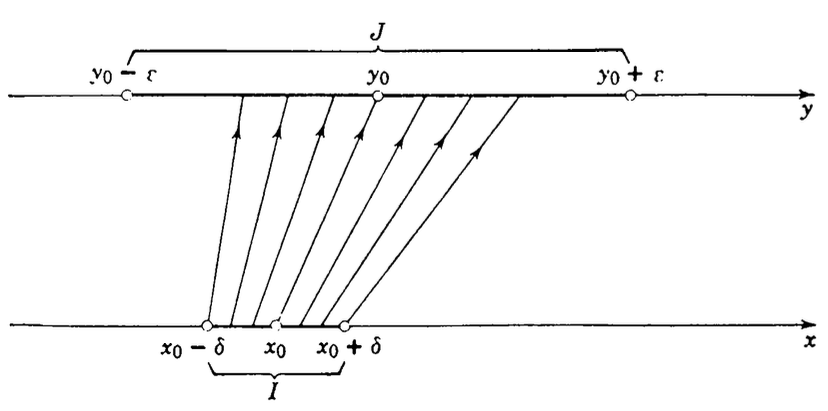
\includegraphics[width=.8\textwidth]{pics/continuidad-1.png}}

Tomemos cualquier punto $x_0$ en el eje $x$ y su imagen $y_0 = f(x_0)$. 
Marcamos un intervalo abierto, arbitrario $J$ en el eje $y$ que tiene al punto $y_0$ como centro; $J = (y_0-\epsilon,y_0+\epsilon) = \{ y \in \R : |y-y_0|<\epsilon\}$.
La condición para la continuidad de $f(x)$ en $x_0$ es: todos los puntos $x$ suficientemente cercanos a $x_0$ tienen imágenes que se encuentran en $J$. O bien: es posible marcar un intervalo $I$ en el eje $x$ con centro $x_0$, por ejemplo, el intervalo $x_0-\delta < x < x_0+\delta$, tal que todo punto $x$ de $I$ tiene una imagen $f(x)$ que se encuentra en $J$ y por lo tanto $|f(x)-f(x_0)|<\epsilon$.
La continuidad de $f(x)$ en el punto $x_0$ significa que para una $\epsilon$-\emph{vecindad} arbitraria $J$ del punto $y_0=f(x_0)$ en el eje $y$, puede encontrarse una $\delta$-vecindad $I$ del punto $x_0$ en el eje $x$, cuya totalidad de puntos son transformados por $f$ en puntos de $J$.
Por supuesto, esto solamente tiene sentido para puntos en el eje $x$ en los cuales la función está definida, esto es, los que pertenecen al dominio de $f$. Lo anterior nos conduce a la siguiente definición.

\begin{definition}\label{D:continuidad}
Sea $f$ definida en un intervalo abierto $(a,b)$ y sea $x_0\in(a,b)$.
    La función $f(x)$ es continua en $x_0$ si se cumple lo siguiente:
    \begin{quote}
        Para cada $\epsilon > 0$, existe $\delta > 0$ tal que
        \[ 
        |f(x) - f(x_0)| < \epsilon,
        \]
        para todos los valores $x$ que cumplen $|x-x_0|<\delta$.
    \end{quote}
\end{definition}

\begin{remark}
    Alternativamente, podemos decirlo de esta otra manera.
    La función $f(x)$ es continua en $x_0$ si se cumple lo siguiente:
    \begin{quote}
        Para cada $\epsilon > 0$, existe $\delta > 0$ tal que
        la imagen por $f$ del conjunto $(x_0-\delta,x_0+\delta)$ está contenida en $(f(x_0)-\epsilon,f(x_0)+\epsilon)$.
    \end{quote}

    O también suele escribirse así:
    La función $f(x)$ es continua en $x_0$ si se cumple lo siguiente:
    \begin{quote}
        Para cada $\epsilon > 0$, existe $\delta > 0$ tal que
        \[ 
        |x-x_0|<\delta \quad\implies\quad |f(x) - f(x_0)| < \epsilon.
        \]
    \end{quote}

\end{remark}

\begin{example}
    Veamos que la función $f(x)=5x+3$ es continua en $x_0 = 2$. Comenzamos, como cuando veíamos límite de sucesiones, analizando la expresión que queremos ver que sea menor a $\epsilon$:
    \[
    |f(x)-f(x_0)|      
    = |f(x)-f(2)|  
    = |(5x+3)-(5\cdot 2 + 3)|  
    = |5x-5\cdot 2 |
    = 5 \, |x-2|.
    \]
    Esta igualdad expresa que la transformación $y=5x+3$ \emph{magnifica} distancias por el factor $5$. Aquí vemos que $|f(x)-f(2)|<\epsilon$ si $5 |x-2| < \epsilon$, o lo que es lo mismo, si $|x-2|<\epsilon/5$.
    Por lo tanto, la condición para la continuidad en $x_0=2$ se verifica si se elige $\delta = \epsilon/5$.

    También podemos verificar que la misma función $f(x)=5x+3$ es continua en todo $x_0\in \R$. Con el mismo razonamiento,
    \[
    |f(x)-f(x_0)|  
    = |(5x+3)-(5 x_0 + 3)|  
    = |5x-5 x_0 |
    = 5 \, |x-x_0|.
    \]
    Luego, se cumplirá que $|f(x)-f(x_0)| <\epsilon$ si $5 \, |x-x_0|<\epsilon$, o lo que es lo mismo, si $|x-x_0|<\epsilon/5$.

    En ambos casos hemos demostrado que dado $\epsilon>0$ existe $\delta>0$ ($\delta=\epsilon/5$) tal que, 
    \[
    \text{si } |x-x_0|<\delta, \quad\text{entonces } |f(x)-f(x_0)|<\epsilon.
    \]
    Es decir, $f(x)=5x+3$ es continua en $x_0$, cualquiera sea $x_0\in\R$.
\end{example}

Veamos otro ejemplo, no tan sencillo.
\begin{example}
    Consideremos la función $f(x)=x^2$. Veamos que es continua en $x_0$ para cualquier $x_0\in\R$. Consideremos $x_0$ fijo, supongamos que $|x-x_0|<\delta$ y veamos qué tiene que cumplir $\delta$ para que se cumpla que $|f(x)-f(x_0)|<\epsilon$:
\begin{align*}
 |f(x)-f(x_0)|  
    &= |x^2 - x_0^2| = |x-x_0| \, |x+x_0|
    = |x-x_0| \, |(x-x_0)+2x_0|
    \\
    &\le |x-x_0| \big( |x-x_0|+2|x_0| \big)
    < \delta \big( \delta + 2 |x_0|\big).
\end{align*}
Ahora queremos elegir $\delta>0$ que asegure que $\delta \big( \delta + 2 |x_0|\big) < \epsilon$. No hace falta elegir el mejor $\delta$, uno que cumpla sería suficiente. Por ejemplo, si elegimos $\delta \le 1$, tenemos
que
\[
\delta \big( \delta + 2 |x_0|\big) \le \delta \big( 1 + 2 |x_0|\big)
< \epsilon, \quad\text{si } \delta \le \frac{\epsilon}{1 + 2 |x_0|}.
\]
Hechos estos \emph{cálculos auxiliares}, procedemos a demostrar que $f(x)=x^2$ es continua en todo punto $x_0$.

Sea $x_0\in\R$. Sea $\epsilon > 0$, arbitrario. Definimos $\delta = \min\{1,\frac{\epsilon}{1 + 2 |x_0|}\}$, de manera que $\delta\le 1$ y $\delta \le \frac{\epsilon}{1 + 2 |x_0|}$. Si $|x-x_0|<\delta$, entonces
\begin{align*}
 |f(x)-f(x_0)|  
    &= |x^2 - x_0^2| = |x-x_0| \, |x+x_0|
    = |x-x_0| \, |(x-x_0)+2x_0|
    \\
    &\le |x-x_0| \big( |x-x_0|+2|x_0| \big)
    < \delta \big( \delta + 2 |x_0|\big)
    \le \delta \big( 1 + 2 |x_0|\big)
< \epsilon.
\end{align*}
Resumiendo, hemos demostrado que dado $\epsilon > 0$, existe $\delta > 0$ tal que 
\[
|f(x)-f(x_0)|<\epsilon, \quad\text{para todo $x\in \R$ tal que $|x-x_0|<\delta$}.
\]
Es decir, $f(x)$ es continua en $x_0$.
\end{example}

\begin{remark}
    En el primer ejemplo, había que tomar $\delta = \frac\epsilon5$, y en el segundo $\delta = \min\{1,\frac{\epsilon}{1 + 2 |x_0|}\}$. Es interesante notar que, en el primer ejemplo, la misma elección de $\delta$ sirve para todo $x_0$, aunque depende de $\epsilon$. 
    En el segundo caso, $\delta$ depende de $\epsilon$ y también de $x_0$, ya que la transformación $y=x^2$ \emph{magnifica} distancias por un factor que no es el mismo para todo $x$.
\end{remark}

Intuitivamente, la idea de la continuidad parece obvia sin explicación, pero la formulación precisa puede ser en un principio algo difícil de entender debido a la variedad de palabras. 
Sin embargo, el lector, que puede estar al principio muy satisfecho con alguna noción intuitiva de la continuidad, aprenderá gradualmente a apreciar la lógica precisión y generalidad de la definición analítica, resultado de un largo y persistente esfuerzo para conciliar la necesidad de entendimiento intuitivo con el de la claridad lógica.
Es indispensable un significado preciso para la palabra continuidad. La definición dada aquí es la formulación requerida y precisa de una importante propiedad de las funciones.

\subsection*{Explicación de continuidad y discontinuidad mediante ejemplos}

Podemos aclarar la definición de continuidad, haciendo contraste con ejemplos de discontinuidad, ejemplos que no satisfacen la definición anterior. Recordemos el ejemplo sencillo de la función $f(x)=\sgn(x)$ en~\eqref{eq:signo}. Si hacemos un gráfico como el anterior, resulta así:

\centerline{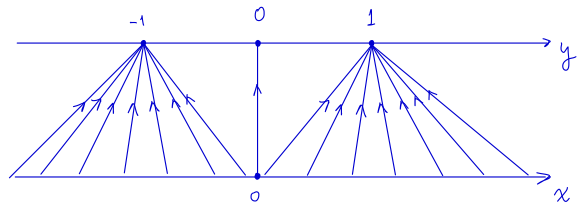
\includegraphics[width=.8\textwidth]{pics/signo.png}}

Esta función es continua en $x_0$, para todo $x_0\neq 0$. Para ver esto, analicemos por separado el caso $x_0>0$ y el caso $x_0<0$.

Sea $x_0 > 0$. Dado $\epsilon>0$, tomemos $\delta = x_0 = |x_0|$ (la distancia de $x_0$ al origen. Entonces, si $|x-x_0|<\delta=|x_0|$ resulta 
\[
0 = x_0-|x_0| < x < x_0+|x_0| = 2 \, |x_0|.
\]
Es decir, $x>0$, luego
\[
|\sgn(x)-\sgn(x_0)| = |1 - 1| = 0 < \epsilon.
\]
Sea ahora $x_0 <0$. Dado $\epsilon>0$, tomemos $\delta = -x_0 = |x_0|$ (la distancia de $x_0$ al origen). Entonces, si $|x-x_0|<\delta=|x_0|$ resulta 
\[
-2|x_0| = x_0-|x_0| < x < x_0+|x_0| = 0.
\]
Es decir, $x<0$, luego
\[
|\sgn(x)-\sgn(x_0)| = |(-1) - (-1)| = 0 < \epsilon.
\]
En síntesis, la función signo es continua en $x_0$, para $x_0>0$ y para $x_0<0$, dado que es constante en $(0,\infty)$ y en $(-\infty,0)$.

¿Qué ocurre en $x_0=0$?
En este caso $\sgn(x_0)=0$.
Para $\epsilon = 1/2$, cualquiera sea $\delta>0$, siempre existe un $x\in (x_0-\delta,x_0+\delta)=(-\delta,\delta)$ para el que $\sgn(x)=1$, por ejemplo, $x=\delta/2$, y para ese $x$ resulta
\[
|\sgn(x)-\sgn(x_0)| = |1 - 0| = 1 > \frac12=\epsilon.
\]

\centerline{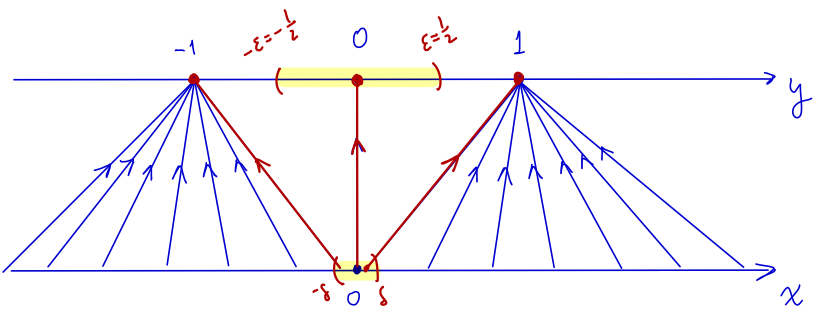
\includegraphics[width=.8\textwidth]{pics/signo-discontinuo.png}}

Es decir, no hay forma de elegir $\delta>0$ suficientemente pequeño para que la imagen por la función signo del intervalo $(-\delta,\delta)$ caiga dentro del intervalo $(-\epsilon,\epsilon)=(-1/2,1/2)$. De hecho, la imagen de $(-\delta,\delta)$ por la función $\sgn(x)$ es siempre el conjunto $\{-1,0,1\}$.

La discontinuidad de la función signo en $x_0=0$ es lo que se conoce como \emph{discontinuidad de salto}, ya que existen los \emph{límites laterales}.
Existe el límite de $f(x)$ cuando $x$ tiende a $0$ por derecha, y es igual a 1, y existe el límite de $f(x)$ cuando $x$ tiende a $0$ por izquierda, y es igual a $-1$. El \emph{salto} es la diferencia de estos límites.

Estamos hablando aquí del concepto de límite, pensando que se entiende intuitivamente lo que significa, pero ya haremos más rigurosa esta definición en la sección siguiente.

Hay otras discontinuidades que no son de salto, son las discontinuidades \emph{infinitas}, que son las que exhiben la función $f(x)=1/x^2$ y la $g(x)=1/x$.

\centerline{
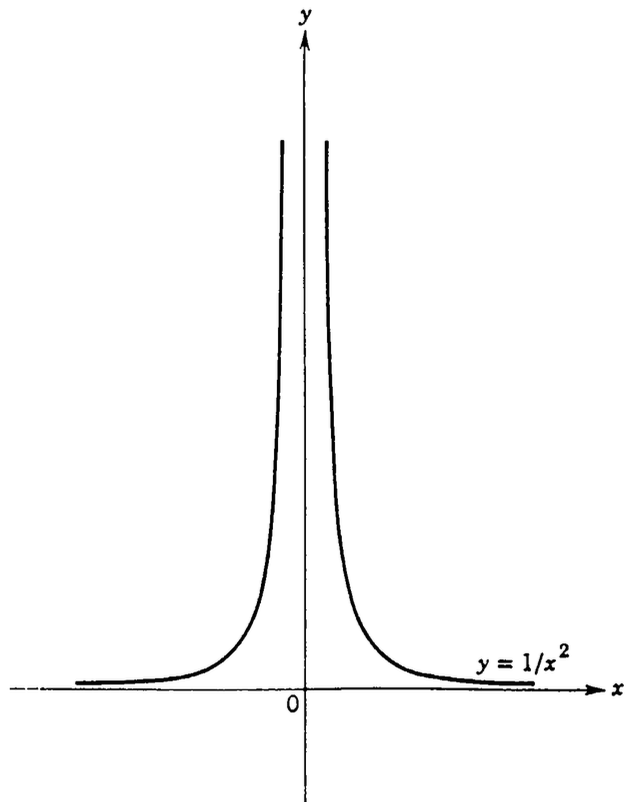
\includegraphics[width=.4\textwidth]{pics/discontinuidad-infinita.png}
\hfil
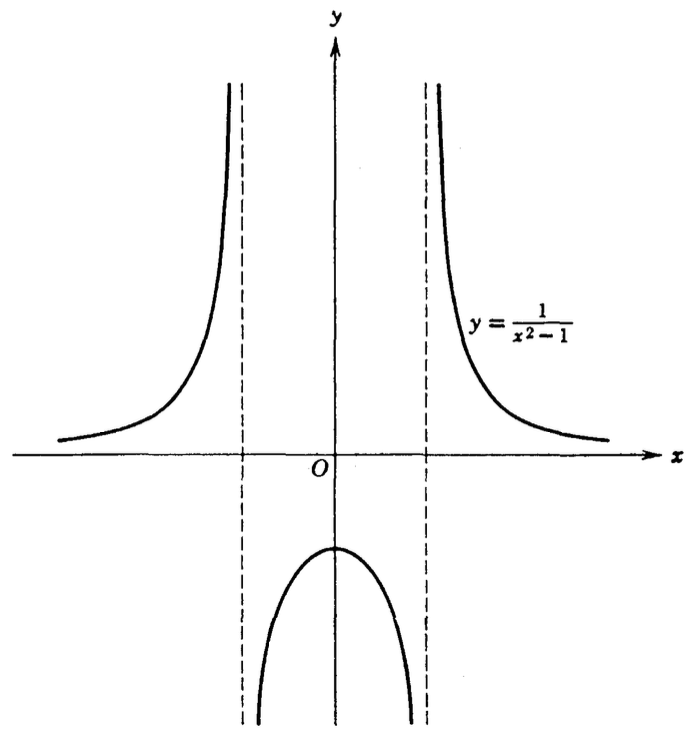
\includegraphics[width=.5\textwidth]{pics/dos-discontinuidades-infinitas.png}
}

A medida que $x$ se aproxima a cero, los valores de $f(x)=1/x^2$ crecen más allá de toda cota. En este caso, diremos que $\D\lim_{x\to0} \frac1{x^2}=\infty.$

\subsubsection*{Ejercicios de la sección~\getcurrentref{chapter}.\getcurrentref{section}}


\begin{enumerate}
\item Demostrar que la función $f(x)=-3x+10$ es continua en $x_0$, para todo $x_0\in\R$.

\item 
Consideremos la función $f:(0,\infty)\to(0,\infty)$ dada por
$f(x)=\frac1x$.
\begin{enumerate}
    \item Demostrar que es continua en $x_0=2$;
    \item Demostrar que es continua en $x_0=1$;
    \item Demostrar que es continua en $x_0=1/2$;
    \item ¿Se anima a demostrar que es continua en $x_0$, cualquiera sea  $x_0>0$?
\end{enumerate}

\item 
Consideremos la función $f:(0,\infty)\to(0,\infty)$ dada por
$f(x)=\sqrt x$.
\begin{enumerate}
    \item Demostrar que es continua en $x_0=2$;
    \item Demostrar que es continua en $x_0=1$;
    \item Demostrar que es continua en $x_0=1/2$;
    % \item Demostrar que es continua en $x_0=0$;
    \item ¿Se anima a demostrar que es continua en $x_0$, cualquiera sea $x_0\in(0,\infty)$?
\end{enumerate}

\item 
Consideremos la función 
\[
f(x) = \begin{cases}
    x\sen \frac1x,\quad &\text{si $x\neq 0$},
    \\
    0,\quad &\text{si $x = 0$},
    \end{cases}
\]
\begin{enumerate}
    \item Graficarla con GeoGebra
    \item Verificar con geogebra que 
    \[
    -|x| \le f(x) \le |x|,\quad \forall\xiR.
    \]
    \item Demostrar analíticamente que 
    \[
    -|x| \le f(x) \le |x|,\quad \forall\xiR.
    \]
    \item Verificar que $|f(x)-f(0)|\le |x-0|$, para todo \xiR.
    \item Demostrar que $f(x)$ es continua en $x_0=0$.
\end{enumerate}

\item 
Consideremos la función
\[
H(x) = \begin{cases}
    0, \quad &\text{si $x<0$},\\
    1, \quad &\text{si $x\ge0$},
\end{cases}
\]
\begin{enumerate}
    \item Demostrar que $H(x)$ es continua en $x_0$ para todo $x_0\neq 0$.
    \item Demostrar que $H(x)$ no es continua en $x_0=0$.
\end{enumerate}

\item \label{ej:sen1_x}
Consideremos la función 
\[
f(x) = \begin{cases}
    \sen \frac1x,\quad &\text{si $x\neq 0$},
    \\
    0,\quad &\text{si $x = 0$},
    \end{cases}
\]
\begin{enumerate}
    \item Graficarla con GeoGebra
    \item Demostrar que para cada $\delta>0$ existe $x_1\in(0,\delta)$ tal que $f(x_1)=1$.
    \item Demostrar que para cada $\delta>0$ existe $x_2\in(0,\delta)$ tal que $f(x_2)=-1$.
    \item Demostrar que $f(x)$ no es continua en $x_0=0$.
\end{enumerate}


\end{enumerate}

\section{Propiedades de funciones continuas en un punto}\label{S:continuidad-propiedades}

A continuación veremos algunas propiedades que cumplen las funciones alrededor de un punto de continuidad.

\begin{proposition}\label{P:continua:cota en intervalo}
    Sea $f$ continua en $x_0$. Si $a<f(x_0)<b$, entonces existe $\delta>0$ tal que 
    \[
    a<f(x)<b, \quad\text{para todo $x\in (x_0-\delta,x_0+\delta)$}.
    \]
\end{proposition}

\begin{proof}
    Basta con tomar $\epsilon=\min\{b-f(x_0),f(x_0)-a\}$ en la definición de continuidad, y elegir el $\delta$ que le corresponde.
\end{proof}

Como consecuencia de esta proposición tenemos que si $f$ es continua en $x_0$ y $f(x_0)>0$, entonces $f$ es positiva en todo un entorno que contiene a $x_0$. Más precisamente, existe $\delta>0$ tal que $f(x)>0$ para todo $x\in (x_0-\delta,x_0+\delta)$.

\begin{proposition}
    Si $f$ y $g$ son continuas en $x_0$, entonces $f+g$ es continua en $x_0$.
\end{proposition}

\begin{proof}
Sea $\epsilon >0$.
Como $f$ es continua en $x_0$ existe $\delta_f>0$ tal que 
\[
|f(x)-f(x_0)|<\frac\epsilon2, \quad\text{para todo $x\in(x_0-\delta_f,x_0+\delta_f)$}.
\]
Como $g$ es continua en $x_0$ existe $\delta_g>0$ tal que 
\[
|g(x)-g(x_0)|<\frac\epsilon2, \quad\text{para todo $x\in(x_0-\delta_g,x_0+\delta_g)$}.
\]
Tomemos ahora $\delta=\min\{\delta_f,\delta_g\}$. Si $x\in(x_0-\delta,x_0+\delta)$, entonces $x\in(x_0-\delta_f,x_0+\delta_f)\cap(x_0-\delta_g,x_0+\delta_g)$.
Por lo tanto, 
\begin{align*}
\Big|\big(f(x)+g(x)\big)-\big(f(x_0)+g(x_0)\big)\Big|
&=\Big|\big(f(x)-f(x_0)\big)+\big(g(x)-g(x_0)\big)\Big|
\\
&\le \big|f(x)-f(x_0)\big|+\big|g(x)-g(x_0)\big|
<\frac\epsilon2+\frac\epsilon2=\epsilon,
\end{align*}
para todo $x\in(x_0-\delta,x_0+\delta)$.

Hemos demostrado que dado $\epsilon>0$, existe $\delta>0$ tal que 
\[
\Big|\big(f(x)+g(x)\big)-\big(f(x_0)+g(x_0)\big)\Big|
<\epsilon , \quad\text{para todo $x\in(x_0-\delta,x_0+\delta)$}.
\]
Es decir, $f+g$ es continua en $x_0$.
\end{proof}


\begin{proposition}
    Si $f$ y $g$ son continuas en $x_0$, entonces $f\cdot g$ es continua en $x_0$.
\end{proposition}

\begin{proof}
    Comencemos observando la diferencia que queremos hacer menor a $\epsilon$:
\begin{align*}
\big|f(x) g(x)-f(x_0) g(x_0)\big|
&=
\big|f(x) g(x)-f(x_0) g(x)+f(x_0) g(x)-f(x_0) g(x_0)\big|
\\
&\le 
\big|f(x) g(x)-f(x_0) g(x)\big|+\big|f(x_0) g(x)-f(x_0) g(x_0)\big|
\\
&\le 
\big|f(x)-f(x_0)\big|\,\big|g(x)\big|+\big|f(x_0)\big| \, \big| g(x)- g(x_0)\big|.
\end{align*}
Vemos que aparecen $|f(x)-f(x_0)|$ y $|g(x)- g(x_0)|$ que podremos acotar por $\epsilon$, pero multiplicados por $|g(x)|$ y por $|f(x_0)|$.
Como $|g(x)|$ todavía depende de $x$ y \emph{no está fijo} debemos acotarlo primero.

Observemos que como $g$ es continua en $x_0$, tomando $\epsilon=1$ en la definición, resulta que existe $\delta_1>0$ tal que
\[
|g(x)-g(x_0)|<1, \quad\text{para todo $x\in(x_0-\delta_1,x_0+\delta_1)$}.
\]
Esto implica que 
\[
|g(x)| < |g(x_0)|+1,  \quad\text{para todo $x\in(x_0-\delta_1,x_0+\delta_1)$}.
\]

Sea ahora $\epsilon>0$ arbitrario.
Llamamos $M=|g(x_0)|+1$ y $N=|f(x_0)|+1$. 
Como $f$ es continua en $x_0$ existe $\delta_f>0$ tal que 
\[
|f(x)-f(x_0)|<\frac{\epsilon}{2M}, \quad\text{para todo $x\in(x_0-\delta_f,x_0+\delta_f)$}.
\]
Como $g$ es continua en $x_0$ existe $\delta_g>0$ tal que 
\[
|g(x)-g(x_0)|<\frac\epsilon{2N}, \quad\text{para todo $x\in(x_0-\delta_g,x_0+\delta_g)$}.
\]

Tomemos ahora $\delta=\min\{\delta_1,\delta_f,\delta_g\}$. Luego,
\[
\text{si $x\in (x_0-\delta,x_0+\delta)$}
\quad\implies\quad
x\in(x_0-\delta_1,x_0+\delta_1)\cap(x_0-\delta_f,x_0+\delta_f)\cap(x_0-\delta_g,x_0+\delta_g).
\]
Por lo tanto, para $x\in (x_0-\delta,x_0+\delta)$ se tiene que
\begin{align*}
\big|f(x) g(x)-f(x_0) g(x_0)\big|
&\le 
\big|f(x)-f(x_0)\big|\,\big|g(x)\big|+\big|f(x_0)\big| \, \big| g(x)- g(x_0)\big|
\\
&< \frac{\epsilon}{2M} M + N \frac\epsilon{2N} = \frac\epsilon2+\frac\epsilon2=\epsilon.
\end{align*}

Hemos demostrado que dado $\epsilon>0$ existe $\delta>0$ tal que
\[
\big|f(x) g(x)-f(x_0) g(x_0)\big|<\epsilon, \quad\text{para todo $x\in(x_0-\delta,x_0+\delta)$}.
\]
Es decir, $fg$ es continua en $x_0$.
\end{proof}

\begin{proposition}
    Si $f$ y $g$ son continuas en $x_0$, 
    y si además $g(x_0)\neq 0$, entonces $f/g$ es continua en $x_0$.
\end{proposition}

\begin{proof}
    Veamos primero que si $g$ es continua en $x_0$ y $g(x_0)\neq 0$, entonces $\D\frac1g$ es continua en $x_0$.
    Para esto, observemos que
    \begin{align*}
        \Big| \frac1{g(x)}-\frac1{g(x_0)} \Big| 
        &= 
        \Big| \frac{g(x_0)-g(x)}{g(x)\,g(x_0)} \Big| 
        = 
         \frac{1}{|g(x)\,g(x_0)|}
        \big| g(x_0)-g(x) | .
    \end{align*}
    Sin pérdida de generalidad, supongamos que $g(x_0)>0$ (el caso $g(x_0)<0$ es análogo).
    Como $g(x_0)>0$, resulta que $0<\frac{g(x_0)}{2}<g(x_0)$. 
    Por la Proposición~\ref{P:continua:cota en intervalo}, existe $\delta_1>0$ tal que 
\[
g(x)>\frac{g(x_0)}2,  \quad\text{para todo $x\in(x_0-\delta_1,x_0+\delta_1)$}.
\] 
Luego, 
\[
\frac{1}{|g(x)\,g(x_0)|} = \frac{1}{g(x)\,g(x_0)}
< \frac{2}{g(x_0)\,g(x_0)}
= \frac{2}{g(x_0)^2},  \quad\text{para todo $x\in(x_0-\delta_1,x_0+\delta_1)$}.
\] 

Sea ahora $\epsilon>0$ arbitrario.
Llamamos $M=\frac{2}{g(x_0)^2}$.
Como $g$ es continua en $x_0$ existe $\delta_g>0$ tal que 
\[
|g(x)-g(x_0)|<\frac\epsilon{M}, \quad\text{para todo $x\in(x_0-\delta_g,x_0+\delta_g)$}.
\]
Tomemos ahora $\delta=\min\{\delta_1,\delta_g\}$. Luego,
\[
\text{si $x\in (x_0-\delta,x_0+\delta)$}
\quad\implies\quad
x\in(x_0-\delta_1,x_0+\delta_1)\cap(x_0-\delta_g,x_0+\delta_g).
\]
Por lo tanto, para $x\in (x_0-\delta,x_0+\delta)$ se tiene que
    \begin{align*}
        \Big| \frac1{g(x)}-\frac1{g(x_0)} \Big| 
        &= 
         \frac{1}{|g(x)\,g(x_0)|}
        \big| g(x_0)-g(x) | 
        < M \frac{\epsilon}M = \epsilon
    \end{align*}

Hemos demostrado que dado $\epsilon>0$ existe $\delta>0$ tal que
\[
        \Big| \frac1{g(x)}-\frac1{g(x_0)} \Big| <\epsilon,
        \quad\text{para todo $x\in(x_0-\delta,x_0+\delta)$}.
\]
Es decir, $\D\frac1g$ es continua en $x_0$.

Finalmente, $\D\frac fg = f \frac1g$. Como $f$ y $\D\frac1g$ son continuas en $x_0$, también lo es su producto por la proposición anterior.
\end{proof}

La siguiente proposición dice que si dos funciones son continuas, entonces también es continua su composición.

\begin{proposition}
    Si $g$ es continua en $x_0$ y $f$ es continua en $g(x_0)$, entonces $f\circ g$ es continua en $x_0$.
\end{proposition}

\begin{proof}
Esta demostración es un poquito más difícil, pero no tanto.
Para hacerla, llamaremos $y$ a la variable independiente de la función $f$.

Sea $\epsilon>0$, como $f$ es continua en $y_0=g(x_0)$, existe $\eta>0$ tal que
\[
|f(y)-f(y_0)|<\epsilon, \quad\text{para todo $y\in(y_0-\eta,y_0+\eta)$},
\]
es decir
\begin{equation}\label{P:composicion-intermedio}
|f(y)-f(y_0)|<\epsilon, \quad\text{si $|y-y_0|<\eta$},
\end{equation}
También hemos utilizado la letra griega $\eta$ (``eta'') en lugar de $\delta$, pero esto no es un problema.

\comentario{Como $\eta>0$, podemos utilizarla en lugar de $\epsilon$ en la definición de continuidad de $g$ en $x_0$.}

Como $g$ es continua en $x_0$ y $\eta>0$, existe $\delta>0$ tal que 
\[
|\underbrace{g(x)}_y-\underbrace{g(x_0)}_{y_0}|<\eta, \quad\text{para todo $x\in(x_0-\delta,x_0+\delta)$}.
\]
Si ahora $x\in(x_0-\delta,x_0+\delta)$, resulta que $y=g(x)$ cumple $|y-y_0|<\eta$ y por lo tanto, de~\eqref{P:composicion-intermedio} tenemos que
\[
|f\circ g(x)-f\circ g(x_0) | 
=\big|f\big(g(x)\big)-f\big(g(x_0)\big) \big| 
=\big|f\big(y\big)-f\big(y_0\big) \big| <\epsilon.
\]

Hemos demostrado que dado $\epsilon>0$ existe $\delta>0$ tal que
\[
        |f\circ g(x)-f\circ g(x_0) |  <\epsilon,
        \quad\text{para todo $x\in(x_0-\delta,x_0+\delta)$}.
\]
Es decir, $f\circ g$ es continua en $x_0$.
\end{proof}

Para continuar hablando de continuidad, conviene introducir el concepto de límite de funciones, lo que haremos en la siguiente sección.

\subsubsection*{Ejercicios de la sección~\getcurrentref{chapter}.\getcurrentref{section}}

\begin{enumerate}
\item Consideremos la función constante $f(x)=a$, para algún $a\in\R$. Demostrar usando la definición que $f$ es continua en $x_0$ para todo $x_0\in\R$.
\item Consideremos la función \emph{identidad} $f(x)=x$. Demostrar usando la definición que $f$ es continua en $x_0$ para todo $x_0\in\R$.
\item Demostrar que si $a$ y $b$ son números reales, entonces la función lineal $f(x)=ax+b$ es continua en $x_0$ para todo $x_0\in\R$.
Usar lo demostrado en los ejercicios anteriores y las propiedades vistas en esta sección.
\item Demostrar que si $a$, $b$ y $c$ son números reales, entonces la función cuadrática $f(x)=ax^2+bx+c$ es continua en $x_0$ para todo $x_0\in\R$.
Usar lo demostrado en los ejercicios anteriores y las propiedades vistas en esta sección.
\item\label{ej:polinomios-continuos} Demostrar que si $p(x)$ es una función polinomial, entonces $p$ es continua en $x_0$ para todo $x_0\in\R$ (Ayuda: usar inducción sobre el grado polinomial).
\item Demostrar que si $p(x)$ y $q(x)$ son funciones polinomiales, entonces la función racional $\frac pq$ es continua en $x_0$ para todo $x_0\in\R$, excepto para aquellos puntos donde $q(x)$ se anula. 


\end{enumerate}


\section{Límites por la derecha}

\subsection{Definición y ejemplos}

Hemos hablado en la sección anterior muy brevemente sobre el concepto de límite. En esta sección presentaremos la definición rigurosa de este concepto y veremos algunos ejemplos.

La idea intuitiva de \emph{límite} de una función $f(x)$ cuando $x$ se acerca a $x_0$ \emph{por derecha}, es el número al que se acercan los valores de $f(x)$ cuando $x$ está arbitrariamente cerca de $x_0$, pero a la derecha de $x_0$, es decir, $x>x_0$. Es importante notar que aquí hemos escrito $x>x_0$ y no $x\ge x_0$. Esto es así, porque no queremos saber el valor de $f(x_0)$, sino el valor al que se acerca $f(x)$ cuando $x$ está cerca de $x_0$, pero $x\neq x_0$.

Por ejemplo, en la función $f(x)=\sgn(x)$ dada en~\eqref{eq:signo}, diremos que límite de $\sgn(x)$ cuando $x$ tiende a cero por derecha es 1, que difiere de $\sgn(0)=0$. En símbolos, escribiremos $\D\lim_{x\to0^+} \sgn(x)=1$.

\begin{definition}[Límite por la derecha]
    Sea $x_0\in\R$ y sea $f$ una función definida en un intervalo $(x_0,x_0+c)$, con $c>0$. Se dice que límite de $f(x)$ cuando $x$ tiende a $x_0$ por derecha es $\ell$ y se escribe
    \[
    \lim_{x\to x_0^+}f(x)=\ell,
    \]
    cuando se cumple lo siguiente:
    \begin{quote}
        Dado $\epsilon > 0$, existe $\delta > 0$ tal que 
        \[
        |f(x)-\ell| < \epsilon, \quad\text{para todo $x\in (x_0,x_0+\delta)$}
        .
        \]
    \end{quote}
\end{definition}
    
\begin{remark}
    En otras palabras
    \[
    \lim_{x\to x_0^+}f(x)=\ell,
    \]
    cuando se cumple lo siguiente:
    \begin{quote}
        Dado $\epsilon > 0$, existe $\delta > 0$ tal que 
        \[
        x_0<x<x_0+\delta
        \quad\implies\quad |f(x)-\ell| < \epsilon.
        \]
    \end{quote}
\end{remark}

\begin{example}
Veamos que con esta definición es cierto que $\D\lim_{x\to0^+} \sgn(x)=1$.
Como la función es constantemente igual a 1 para $x>0$, la elección de $\delta$ será muy sencilla; en realidad cualquier $\delta>0$ sirve, pero para ser explícitos, tomaremos $\delta=1$.\footnote{Queremos evitar aquí el problema que le surgió a Homero Simpson, cuando la computadora le pedía que ``TO START PRESS ANY KEY", y no encontraba la tecla ``ANY"  (\url{https://www.youtube.com/watch?v=st6-DgWeuos}\quad:-)}

Sea $\epsilon > 0$, tomemos $\delta=1$, luego, si $0<x<\delta=1$, resulta que
\[
|\sgn(x)-1| = |1-1|=0<\epsilon,
\]
donde hemos utilizado solamente que $x>0$, ignorando que $x<1$.
Hemos demostrado entonces que dado $\epsilon>0$ existe $\delta>0$ con la propiedad de que
\[
0<x<0+\delta \quad\implies\quad |\sgn(x)-1|<\epsilon,
\]
es decir, $\D\lim_{x\to0^+} \sgn(x)=1$.
\end{example}

\begin{example}
Consideremos la función $f:\R\to\R$ definida por $f(x)=\lfloor x\rfloor$, la función \emph{parte entera de $x$}, o también llamada \emph{piso de $x$}.
Es decir, $f(x)$ es el único entero que cumple $f(x)\le x< f(x)+1$. Así, $f(x)=0$, para todo $x\in[0,1)$, $f(x)=1$, para todo $x\in[1,2)$, etc. En general
\[
f(x)=n, \qquad \text{si }n\in\Z \quad\text{y}\quad n\le x < n+1.
\]
Veamos que el límite de $f(x)$ cuando $x$ tiende a $3$ por derecha es $3$, es decir, $\lim_{x\to 3^+}f(x)=3$.
Observamos que $f$ es constante en el intervalo $[3,4)$, por lo tanto, lo que ocurre es similar a lo que ocurre con la función signo.
Sea $\epsilon>0$, elegimos $\delta=1$ y observamos que si $3<x<3+\delta=4$ entonces $f(x)=3$,
por lo tanto
\[
|f(x)-3| = |3-3|=0<\epsilon,\quad\text{para todo $x\in (3,3+\delta)$}.
\]
De la misma manera, cambiando $3$ por $n$ y $4$ por $n+1$ podemos probar que si $n\in\Z$, entonces $\lim_{x\to n^+}f(x)=n$.

Consideremos ahora un número $x_0\in \R\setminus\Z$, es decir, $x_0$ es real, pero no entero. Entonces, si tomamos $n=\lfloor x_0 \rfloor$, resulta que
$n\in\Z$ y $n<x_0<n+1$, donde ambas desigualdades son \emph{estrictas}, porque $x_0$ no es entero.
Además, $f(x_0)=n$, y si ampliamos el gráfico alrededor del punto $(x_0,n)=(x_0,f(x_0))$, vemos que la función $f$ es constante alrededor de $x_0$.
Dado $\epsilon>0$, ?`cómo tenemos que elegir $\delta>0$ de manera de asegurarnos que $|f(x)-f(x_0)|<\epsilon$ para todo $x\in(x_0,x_0+\delta)$?
Bien, tenemos que asegurarnos que si $x\in(x_0,x_0+\delta)$ entonces $x$ \emph{no se pase a la derecha de $n+1$}.
Para eso, podemos definir $\delta=n+1-x_0$ que es positivo porque ya dijimos que $x_0<n+1$. Luego, si
$x\in(x_0,x_0+\delta)$, resulta $x_0<x<x_0+\delta = x_0+(n+1-x_0)=n+1$, es decir $x_0<x<n+1$ y por lo tanto $f(x)=\lfloor x \rfloor = n = f(x_0)$, que a su vez implica
\[
|f(x)-f(x_0)|=|n-n|=0<\epsilon.
\]
Por lo tanto, dado $\epsilon>0$ existe $\delta=n+1-x_0>0$ tal que $|f(x)-f(x_0)|<\epsilon$ para todo $x\in(x_0,x_0+\delta)$. Es decir, $\lim_{x\to x_0^+}f(x)=f(x_0)$.
\end{example}

\begin{example}
    Consideremos ahora la función definida por $f(x)=\frac{4x^2-100}{x-5}$ cuyo dominio es $\R\setminus\{5\}$.
    Igualmente podemos calcular el límite de $f(x)$ cuando $x$ tiende a $5$ por derecha.
    Afirmamos que $\lim_{x\to 5^+} f(x) = 40$. Esto surge de observar que si $x\neq 5$, entonces
    \[
    f(x) = \frac{4x^2-100}{x-5} = 4\frac{x^2-5^2}{x-5} = 4\frac{(x-5)(x+5)}{x-5} = 4(x+5)\qquad\text{(para $x\neq 5$).}
    \]
    
    Es decir, $f(x)=4(x+5)$, para $x\neq 5$. Si miramos esta fórmula para $x$ cercano a 5, vemos que los valores $4(x+5)$ están cercanos a $4(5+5)=40$.
    Veamos que se cumple la definición formal.
    Sea $\epsilon > 0$, supongamos que $5<x<5+\delta$, es decir $0<x-5<\delta$ y veamos qué ocurre con $|f(x)-40|$. Queremos descubrir qué tiene que cumplir $\delta$ para que $|f(x)-40|<\epsilon$:
    \[
    |f(x)-40|=\left|\frac{4x^2-100}{x-5}-10\right|=|4(x+5)-40|=|4x-20|=4(x-5)<4\delta.
    \]
    Si tomamos $\delta=\epsilon/4$ (para que $4\delta=\epsilon$) resultará que
    \[
    |f(x)-40| < \epsilon, \qquad\text{para todo $x \in (5,5+\delta)$}.
    \]
    Hemos demostrado que dado $\epsilon > 0$ existe $\delta=\epsilon/4$ tal que $|f(x)-40| < \epsilon$, para todo $x \in (5,5+\delta)$.
    Es decir, $\lim_{x\to 5^+} f(x) = 40$.
\end{example}

Terminamos esta sección probando dos propiedades que parecen obvias, pero nos permiten practicar y asimilar la definición de límite.

\begin{lemma}
    Si $f$ es la función \emph{constante}, $f(x)=c$, para todo $x\in\R$, entonces 
    \[ 
    \lim_{x\to x_0^+} f(x) = c, \qquad\text{cualquiera sea $x_0\in\R$}.
    \]
\end{lemma}

\begin{proof}
    Dado $\epsilon>0$, elegimos $\delta=1$ y se cumple que
    \[
    |f(x)-c|=|c-c|=0<\epsilon, \quad\text{para todo $x\in(x_0,x_0+\delta)$}.
    \qedhere \]
\end{proof}

\begin{proposition}
    Si $\lim_{x\to x_0^+} f(x) = \ell$, entonces $\lim_{x\to x_0^+} |f(x)|=|\ell|$.
\end{proposition}

\begin{proof}
    Como $\limxo f(x)=\ell$, dado $\epsilon>0$ existe $\delta>0$ tal que $| f(x)-\ell |<\epsilon$ para todo $x\in(x_0,x_0+\delta)$.
    Pero entonces, si $x\in(x_0,x_0+\delta)$, por la desigualdad triangular, resulta que
    \[
    \big| |f(x)|-|\ell| \big| \le \big| f(x)-\ell \big|<\epsilon.
    \qedhere
    \]
\end{proof}


\subsection{Propiedades del límite por la derecha}


A continuación veremos algunas propiedades del límite que nos permitirán calcularlos sin necesidad de recurrir siempre a la definición.

\begin{proposition}[Unicidad del límite]
    Sea $f$ definida en $(x_0,x_0+c)$ para algún $c>0$. Si $\ell_1$ y $\ell_2$ cumplen que
    \[
    \lim_{x\to x_0^+} f(x)=\ell_1, 
    \qquad \text{y}\qquad 
    \lim_{x\to x_0^+} f(x)=\ell_2,
    \]
    entonces $\ell_1=\ell_2$.
\end{proposition}

\begin{proof}
Sea $\epsilon>0$. 
Como $\lim_{x\to x_0^+} f(x)=\ell_1$, existe $\delta_1$ tal que
\[
|f(x)-\ell_1| < \frac{\epsilon}2, \qquad\text{ para todo $x\in(x_0,x_0+\delta_1)$}.
\]
Como $\lim_{x\to x_0^+} f(x)=\ell_2$, existe $\delta_1$ tal que
\[
|f(x)-\ell_2| < \frac{\epsilon}2, \qquad\text{ para todo $x\in(x_0,x_0+\delta_2)$}.
\]
Si ahora $x\in(x_0,x_0+\min\{\delta_1,\delta_2\}$ tenemos que 
\[
|f(x)-\ell_1| < \frac{\epsilon}2
\quad\text{y}\quad
|f(x)-\ell_2| < \frac{\epsilon}2.
\]
Entonces
\begin{align*}
|\ell_1-\ell_2|&=|\ell_1-f(x)+f(x)-\ell_2|
\le |\ell_1-f(x)|+|f(x)-\ell_2|
\\
&= |f(x)-\ell_1|+|f(x)-\ell_2|
< \frac\epsilon2+\frac\epsilon2=\epsilon.
\end{align*}

Hemos demostrado que $|\ell_1-\ell_2|<\epsilon$, para todo $\epsilon>0$.
Luego $|\ell_1-\ell_2|=0$, o lo que es lo mismo $\ell_1=\ell_2$.
\end{proof}

\begin{proposition}\label{P:limite implica valores acotados}
    Supongamos que $\lim_{x\to x_0^+} f(x)=\ell$.
    \begin{enumerate}
        \item Si $\ell<b$, existe $\delta>0$ tal que $f(x)<b$, para todo $x\in(x_0,x_0+\delta)$.
        \item Si $\ell>b$, existe $\delta>0$ tal que $f(x)>b$, para todo $x\in(x_0,x_0+\delta)$.
    \end{enumerate}
\end{proposition}

\begin{proof}
Basta con tomar $\epsilon = |b-\ell|$ en la definición de límite.
\end{proof}

\begin{theorem}[Teorema del Emparedado]
    Sean $f$, $g$ y $h$ tres funciones definidas en $(x_0,x_0+c)$ para algún $c>0$, tales que
    \begin{enumerate}
        \item $\D\lim_{x\to x_0^+} g(x) = \lim_{x\to x_0^+} h(x) = \ell$;
        \item $g(x)\le f(x) \le h(x)$, para todo $x\in(x_0,x_0+c)$.
    \end{enumerate}
    Entonces $\D \lim_{x\to x_0^+} f(x)=\ell$.
\end{theorem}

\begin{proof}
Sea $\epsilon>0$.
Como $\D\lim_{x\to x_0^+} g(x)=\ell$, existe $\delta_g>0$ tal que
\[
\ell-\epsilon < g(x) < \ell+\epsilon, \qquad\text{ para todo $x\in(x_0,x_0+\delta_g)$}
\]
Como $\D\lim_{x\to x_0^+} h(x)=\ell$, existe $\delta_g>0$ tal que
\[
\ell-\epsilon < h(x) < \ell+\epsilon, \qquad\text{ para todo $x\in(x_0,x_0+\delta_h)$}
\]
Tomemos $\delta=\min\{\delta_g,\delta_h\}$.
Si $x\in(x_0,x_0+\delta)$, entonces $x\in(x_0,x_0+\delta_g)\cap(x_0,x_0+\delta_h)$, luego
\[
\ell-\epsilon < g(x)\le f(x) \le h(x)< \ell+\epsilon.
\]

Hemos demostrado que dado $\epsilon>0$ existe $\delta>0$ tal que 
\[
\ell-\epsilon < f(x)< \ell+\epsilon,
\qquad\text{ para todo $x\in(x_0,x_0+\delta)$},
\]
o lo que es lo mismo
\[
|f(x)-\ell| < \epsilon,
\qquad\text{ para todo $x\in(x_0,x_0+\delta)$}.
\]
Por lo tanto, $\lim_{x\to x_0^+}f(x)=\ell$
\end{proof}

El siguiente teorema permite relacionar el concepto de límite de sucesiones con el de límites de una variable continua.

\begin{theorem}[Teorema fundamental del límite]\label{T:TFLD}
Sea $f$ una función definida en $(x_0,x_0+c)$ para algún $c>0$.
Entonces 
\[ \D \limxop f(x)=\ell
\]
si y sólo si 
\begin{quote}
    para toda sucesión $\big(x_n\big)_{n\in\N}$ tal que $\D\lim_{n\to\infty} x_n = x_0$ con $x_n > x_0$, para todo \niN, vale que $\lim_{n\to\infty}f(x_n)=\ell$.
\end{quote}
\end{theorem}

\begin{proof}
Supongamos primero que $\limxop f(x)=\ell$ y sea $\big(x_n\big)_{n\in\N}$ una sucesión tal que $\D\lim_{n\to\infty} x_n = x_0$ con $x_n > x_0$, para todo \niN.
Sea $\epsilon>0$, entonces, como $\limxop f(x)=\ell$ existe $\delta>0$ tal que
\[
x_0< x <x_0+\delta\quad\implies\quad |f(x)-\ell|<\epsilon.
\]
Ahora bien, como $\D\lim_{n\to\infty} x_n = x_0$, para ese $\delta>0$, existe $N_0\in\N$ tal que
\[
|x_n-x_0|<\delta, \quad\text{para todo $n\ge N_0$}.
\]
Como además $x_n > x_0$, para todo \niN, resulta que 
\[
x_0 < x_n < x_0 + \delta, \quad\text{para todo $n\ge N_0$}.
\]
Luego, $\D |f(x_n)-\ell|<\epsilon, \quad\text{para todo $n\ge N_0$}$.

Hemos probado que dado $\epsilon>0$ existe $N_0\in\N$ tal que 
\[
|f(x_n)-\ell|<\epsilon, \quad\text{para todo $n\ge N_0$}.
\]
Es decir, $\D\lim_{n\to\infty}f(x_n) = \ell$.

Para probar la recíproca, supongamos que para toda sucesión $\big(x_n\big)_{n\in\N}$ tal que $\D\lim_{n\to\infty} x_n = x_0$ con $x_n > x_0$ para todo \niN, vale que $\lim_{n\to\infty}f(x_n)=\ell$.
Debemos probar que $\D\limxop f(x)=\ell$.
Si esto no fuera cierto, entonces existiría $\epsilon>0$ tal que, cualquiera sea $\delta>0$, hay un $x$ que cumple $x_0<x<\delta$ y $|f(x)-\ell|\ge \epsilon$.
Usaremos esta propiedad para construir una sucesión que no cumple lo que supusimos y así llegar a una contradicción.
Tomamos, para cada $n\in\N$, $\delta=\frac1n$ y sea $x_n$ el correspondiente que cumple que $x_0<x_n<x_0+\frac1n$ y $|f(x_n)-\ell|\ge \epsilon$.
De esta manera, hemos construido una sucesión $\big(x_n\big)_{n\in\N}$ tal que $\D\lim_{n\to\infty} x_n = x_0$, con $x_n> x_0$, para todo \niN, para la cual no es cierto que $\lim_{n\to\infty}f(x_n)=\ell$. Esto contradice nuestra suposición, por lo que $\D\limxop f(x)=\ell$.
\end{proof}

Este teorema es muy útil para desarrollar muchas propiedades del límite. Pero en particular es muy útil para demostrar cuando el límite no existe.


\begin{example}
    Veamos que no existe $\D\lim_{x\to 0^+} \sen \frac1x$.
    
    Tomemos en primer lugar la sucesión \sucxn dada por $ x_n = \frac{1}{n\pi}$, que cumple $x_n>0$, $\forall \niN$ y $x_n\to 0$. Además, $\sen\frac1{x_n}=\sen (n\pi) = 0$, para todo \niN. Luego, 
    \[ \lim_{n\to\infty} \sen \frac1{x_n} = 0. \]

    Consideremos ahora la sucesión \sucyn dada por $y_n = \frac{1}{\frac\pi2+2n\pi}$, que cumple $y_n>0$, $\forall \niN$ y $y_n\to 0$. 
    Además, $\sen\frac1{y_n}=\sen (\frac \pi2 + 2n\pi) = 1$, para todo \niN. Luego, 
    \[
    \lim_{n\to\infty} \sen \frac1{y_n} = 1.
    \]

    Hemos encontrado dos sucesiones distintas \sucxn y \sucyn que cumplen $x_n>0$, $y_n>0$ y ambas con límite $0$, para las cuales $\D\lim \sen\frac1{x_n}\neq\lim \sen\frac1{y_n}$. Si existiera $\D\lim_{x\to 0^+} \sen \frac1x$, ambos límites deberían coincidir. Como no coinciden, concluimos que no existe $\D\lim_{x\to 0^+} \sen \frac1x$.
\end{example}

Ahora sí, veamos algunas propiedades de la nueva noción de límite, que pueden probarse como consecuencia de lo que ya sabemos para el límite de sucesiones, usando el Teorema~\ref{T:TFLD}

\begin{proposition}
    Sean $f$ y $g$ dos funciones tales que
    \[
    \lim_{x\to x_0^+} f(x)=\ell_1,
    \qquad
    \lim_{x\to x_0^+} g(x)=\ell_2.
    \]
    Entonces
    \begin{itemize}
        \item $\D \lim_{x\to x_0^+} \big( f(x) + g(x) \big) = \ell_1 + \ell_2$;
        \item $\D \lim_{x\to x_0^+} \big( f(x) \cdot g(x) \big) = \ell_1 \cdot \ell_2$;
        \item Si $\ell_2\neq 0$, $\D \lim_{x\to x_0^+} \frac{f(x)}{g(x)} = \frac{\ell_1}{\ell_2}$.
    \end{itemize}
\end{proposition}

\begin{proof}
Probaremos la primera afirmación de la proposición, las otras son similares.

    Sea \sucxn una sucesión tal que $\D\lim_{n\to\infty} x_n = x_0$ con $x_n > x_0$, para todo \niN.
    Luego, por el Teorema~\ref{T:TFLD}, resulta que
    \[
    \lim_{n\to\infty } f(x_n) = \ell_1,
    \qquad\text{y}\qquad
    \lim_{n\to\infty } g(x_n) = \ell_2.
    \]
    Por lo tanto, usando la propiedad del límite de la suma para sucesiones obtenemos que
    \[
    \lim_{n\to\infty } \big(f(x_n) + g(x_n)\big) = \ell_1+\ell_2.
    \]

    Como la \sucxn era arbitraria, concluimos que $\D  \lim_{n\to\infty } \big(f(x_n) + g(x_n)\big) = \ell_1+\ell_2$
    para toda sucesión \sucxn tal que $\D\lim_{n\to\infty} x_n = x_0$ con $x_n > x_0$, para todo \niN.
    Por el Teorema~\ref{T:TFLD}, resulta que $\D\limxop \big(f(x)+g(x)\big) = \ell_1+\ell_2$.
\end{proof}
\begin{comment} %demostración alternativa usando la definición
\comentario{La demostración de esta proposición es similar a la demostración de que si $f$ y $g$ son continuas en $x_0$, entonces $f+g$ es continua en $x_0$.}

\begin{proof}
Sea $\epsilon >0$.
Como $ \lim_{x\to x_0^+} f(x)=\ell_1$ existe $\delta_f>0$ tal que 
\[
|f(x)-\ell_1|<\frac\epsilon2, \quad\text{para todo $x\in(x_0,x_0+\delta_f)$}.
\]
Como $\lim_{x\to x_0^+} g(x)=\ell_2$ existe $\delta_g>0$ tal que 
\[
|g(x)-\ell_2|<\frac\epsilon2, \quad\text{para todo $x\in(x_0,x_0+\delta_g)$}.
\]
Tomemos ahora $\delta=\min\{\delta_f,\delta_g\}$. Si $x\in(x_0,x_0+\delta)$, entonces $x\in(x_0,x_0+\delta_f)\cap(x_0,x_0+\delta_g)$.
Por lo tanto, 
\begin{align*}
\Big|\big(f(x)+g(x)\big)-\big(\ell_1+\ell_2\big)\Big|
&=\Big|\big(f(x)-\ell_1\big)+\big(g(x)-\ell_2\big)\Big|
\\
&\le \big|f(x)-\ell_1\big|+\big|g(x)-\ell_2\big|
<\frac\epsilon2+\frac\epsilon2=\epsilon,
\end{align*}
para todo $x\in(x_0,x_0+\delta)$.

Hemos demostrado que dado $\epsilon>0$, existe $\delta>0$ tal que 
\[
\Big|\big(f(x)+g(x)\big)-\big(\ell_1+\ell_2\big)\Big|
<\epsilon , \quad\text{para todo $x\in(x_0,x_0+\delta)$}.
\]
Es decir, $\D\lim_{x\to x_0^+} \big( f(x) + g(x) \big) = \ell_1 + \ell_2$.
\end{proof}
\begin{proposition}
    Sean $f$ y $g$ dos funciones tales que
    \[
    \lim_{x\to x_0^+} f(x)=\ell_1,
    \qquad
    \lim_{x\to x_0^+} g(x)=\ell_2.
    \]
    Entonces
    \[ 
    \lim_{x\to x_0^+} \big( f(x) \cdot g(x) \big) = \ell_1 \cdot \ell_2.
    \]
\end{proposition}

\comentario{La demostración de esta proposición es similar a la demostración de que si $f$ y $g$ son continuas en $x_0$, entonces $f\cdot g$ es continua en $x_0$.}

\begin{proof}
    Comencemos observando la diferencia que queremos hacer menor a $\epsilon$:
\begin{align*}
\big|f(x) g(x)-\ell_1 \ell_2\big|
&=
\big|f(x) g(x)-\ell_1 g(x)+\ell_1 g(x)-\ell_1 \ell_2\big|
\\
&\le 
\big|f(x) g(x)-\ell_1 g(x)\big|+\big|\ell_1 g(x)-\ell_1 \ell_2\big|
\\
&\le 
\big|f(x)-\ell_1\big|\,\big|g(x)\big|+\big|\ell_1\big| \, \big| g(x)- \ell_2\big|.
\end{align*}
Vemos que aparecen $|f(x)-\ell_1|$ y $|g(x)- \ell_2|$ que podremos acotar por $\epsilon$, pero multiplicados por $|g(x)|$ y por $|\ell_1|$.
Como $|g(x)|$ todavía depende de $x$ y \emph{no está fijo} debemos acotarlo primero.

Observemos que como $\lim_{x\to x_0^+} g(x)=\ell_2$ es continua en $x_0$, tomando $\epsilon=1$ en la definición, resulta que existe $\delta_1>0$ tal que
\[
|g(x)-\ell_2|<1, \quad\text{para todo $x\in(x_0,x_0+\delta_1)$}.
\]
Esto implica que 
\[
|g(x)| < |\ell_2|+1,  \quad\text{para todo $x\in(x_0,x_0+\delta_1)$}.
\]

Sea ahora $\epsilon>0$ arbitrario.
Llamamos $M=|\ell_2|+1$ y $N=|\ell_1|+1$. 
Como $\lim_{x\to x_0^+} f(x)=\ell_1$ existe $\delta_f>0$ tal que 
\[
|f(x)-\ell_1|<\frac{\epsilon}{2M}, \quad\text{para todo $x\in(x_0,x_0+\delta_f)$}.
\]
Como $\lim_{x\to x_0^+} g(x)=\ell_2$ existe $\delta_g>0$ tal que 
\[
|g(x)-\ell_2|<\frac\epsilon{2N}, \quad\text{para todo $x\in(x_0,x_0+\delta_g)$}.
\]

Tomemos ahora $\delta=\min\{\delta_1,\delta_f,\delta_g\}$. Luego,
\[
\text{si $x\in (x_0,x_0+\delta)$}
\quad\implies\quad
x\in(x_0,x_0+\delta_1)\cap(x_0,x_0+\delta_f)\cap(x_0,x_0+\delta_g).
\]
Por lo tanto, para $x\in (x_0,x_0+\delta)$ se tiene que
\begin{align*}
\big|f(x) g(x)-\ell_1 \ell_2\big|
&\le 
\big|f(x)-\ell_1\big|\,\big|g(x)\big|+\big|\ell_1\big| \, \big| g(x)- \ell_2\big|
\\
&< \frac{\epsilon}{2M} M + N \frac\epsilon{2N} = \frac\epsilon2+\frac\epsilon2=\epsilon.
\end{align*}

Hemos demostrado que dado $\epsilon>0$ existe $\delta>0$ tal que
\[
\big|f(x) g(x)-\ell_1 \ell_2\big|<\epsilon, \quad\text{para todo $x\in(x_0,x_0+\delta)$}.
\]
Es decir, $\D\lim_{x\to x_0^+} \big( f(x) \cdot g(x) \big) = \ell_1 \cdot \ell_2$.
\end{proof}

\begin{proposition}
    Sean $f$ y $g$ dos funciones tales que
    \[
    \lim_{x\to x_0^+} f(x)=\ell_1,
    \qquad
    \lim_{x\to x_0^+} g(x)=\ell_2,
    \]
    y supongamos que $\ell_2\neq 0$.
    Entonces
    \[ 
    \lim_{x\to x_0^+} \frac{f(x)}{g(x)} = \frac{\ell_1}{\ell_2}.
    \]
\end{proposition}


\comentario{La demostración de esta proposición es similar a la demostración de que si $f$ y $g$ son continuas en $x_0$ y $g(x_0)\neq 0$, 
entonces $f/g$ es continua en $x_0$.}

\begin{proof}
    Veamos primero que si $\lim_{x\to x_0^+} g(x)=\ell_2$ y $\ell_2\neq 0$, entonces $\D\lim_{x\to x_0^+} \frac1{g(x)}=\frac1{\ell_2}$.
    Para esto, observemos que
    \begin{align*}
        \Big| \frac1{g(x)}-\frac1{\ell_2} \Big| 
        &= 
        \Big| \frac{\ell_2-g(x)}{g(x)\,\ell_2} \Big| 
        = 
         \frac{1}{|g(x)\,\ell_2|}
        \big| \ell_2-g(x) | .
    \end{align*}
    Sin pérdida de generalidad, supongamos que $\ell_2>0$ (el caso $\ell_2<0$ es análogo).
    Como $\ell_2>0$, resulta que $0<\frac{\ell_2}{2}<\ell_2$. 
    Por la Proposición~\ref{P:limite implica valores acotados}, existe $\delta_1>0$ tal que 
\[
g(x)>\frac{\ell_2}2,  \quad\text{para todo $x\in(x_0,x_0+\delta_1)$}.
\] 
Luego, 
\[
\frac{1}{|g(x)\,\ell_2|} = \frac{1}{g(x)\,\ell_2}
< \frac{2}{\ell_2\,\ell_2}
= \frac{2}{\ell_2^2},  \quad\text{para todo $x\in(x_0,x_0+\delta_1)$}.
\] 

Sea ahora $\epsilon>0$ arbitrario.
Llamamos $M=\frac{2}{\ell_2^2}$.
Como $\lim_{x\to x_0^+} g(x)=\ell_2$ existe $\delta_g>0$ tal que 
\[
|g(x)-\ell_2|<\frac\epsilon{M}, \quad\text{para todo $x\in(x_0,x_0+\delta_g)$}.
\]
Tomemos ahora $\delta=\min\{\delta_1,\delta_g\}$. Luego,
\[
\text{si $x\in (x_0,x_0+\delta)$}
\quad\implies\quad
x\in(x_0,x_0+\delta_1)\cap(x_0,x_0+\delta_g).
\]
Por lo tanto, para $x\in (x_0,x_0+\delta)$ se tiene que
    \begin{align*}
        \Big| \frac1{g(x)}-\frac1{\ell_2} \Big| 
        &= 
         \frac{1}{|g(x)\,\ell_2|}
        \big| \ell_2-g(x) | 
        < M \frac{\epsilon}M = \epsilon
    \end{align*}

Hemos demostrado que dado $\epsilon>0$ existe $\delta>0$ tal que
\[
        \Big| \frac1{g(x)}-\frac1{\ell_2} \Big| <\epsilon,
        \quad\text{para todo $x\in(x_0,x_0+\delta)$}.
\]
Es decir, $\D\lim_{x\to x_0^+} \frac1{g(x)}=\frac1{\ell_2}$.

Finalmente, 
\[
\lim_{x\to x_0^+} f(x)g(x) = \lim_{x\to x_0^+} f(x) \frac1{g(x)}
= \lim_{x\to x_0^+} f(x) \lim_{x\to x_0^+} \frac1{g(x)}
= \ell_1 \, \frac1{\ell_2}.
\qedhere
\]
\end{proof}
\end{comment}


\subsubsection*{Ejercicios de la sección~\getcurrentref{chapter}.\getcurrentref{section}}

\begin{enumerate}
\item Demostrar usando la definición, que $\D\lim_{x\to 0^+} \sqrt{x} = 0$.

\item Demostrar usando el Teorema~\ref{T:TFLD} que no existe $\D\lim_{x\to 0^+}\cos\frac1x$.

\item Determinar (usando los límites que ya conocemos y las propiedades) los siguientes límites, considerando separadamente los casos $x_0\in\Z$ y $x_0\in\R\setminus\Z$:
\begin{multicols}{2}
    \begin{enumerate}
    \item $\D\lim_{x\to x_0^+} \big(x-\lfloor x \rfloor\big)$;
    \item $\D\lim_{x\to x_0^+} \big(|x|+\lfloor x \rfloor\big)$.
    \end{enumerate}
\end{multicols}

\item Determinar (usando los límites que ya conocemos y las propiedades) los siguientes límites, considerando separadamente los casos $x_0=0$ y $x_0\neq 0$:
\begin{multicols}{2}
    \begin{enumerate}
    \item $\D\lim_{x\to x_0^+} \big(x+\sgn(x))$;
    \item $\D\lim_{x\to x_0^+} \big(x\cdot \sgn(x)\big)$.
    \end{enumerate}
    \end{multicols}

\item Demostrar que $\D\lim_{x\to 0^+} x \sen\frac1x = 0$ (?`qué teorema conviene usar para esto?).
    

\end{enumerate}

\section{Límites por la izquierda}

\subsection{Definición y ejemplos}

\begin{definition}[Límite por la izquierda]
    Sea $x_0\in\R$ y sea $f$ una función definida en un intervalo $(x_0-c,x_0)$, con $c>0$. Se dice que límite de $f(x)$ cuando $x$ tiende a $x_0$ por izquierda es $\ell$ y se escribe
    \[
    \lim_{x\to x_0}f(x)=\ell,
    \]
    cuando se cumple lo siguiente:
    \begin{quote}
        Dado $\epsilon > 0$, existe $\delta > 0$ tal que 
        \[
        |f(x)-\ell| < \epsilon, \quad\text{para todo $x\in (x_0-\delta,x_0)$}
        .
        \]
    \end{quote}
\end{definition}

\begin{remark}
        En otras palabras
    \[
    \lim_{x\to x_0}f(x)=\ell,
    \]
    cuando se cumple lo siguiente:
    \begin{quote}
        Dado $\epsilon > 0$, existe $\delta > 0$ tal que 
        \[
        x_0-\delta<x<x_0
        \quad\implies\quad |f(x)-\ell| < \epsilon.
        \]
    \end{quote}
\end{remark}

\begin{example}
Veamos que con esta definición es cierto que $\D\lim_{x\to0^-} \sgn(x)=-1$.
Como la función es constantemente igual a $-1$ para $x<0$, la elección de $\delta$ será muy sencilla; en realidad cualquier $\delta>0$ sirve, pero para ser explícitos, tomaremos $\delta=1$.

Sea $\epsilon > 0$, tomemos $\delta=1$, luego, si $0-\delta<x<0$, resulta que $-1<x<0$
\[
|\sgn(x)-(-1)| = |-1-(-1)|=0<\epsilon,
\]
donde hemos utilizado solamente que $x<0$, ignorando que $x>-1$.
Hemos demostrado entonces que dado $\epsilon>0$ existe $\delta>0$ con la propiedad de que
\[
0-\delta<x<0 \quad\implies\quad |\sgn(x)-(-1)|<\epsilon,
\]
es decir, $\D\lim_{x\to0^-} \sgn(x)=-1$.
\end{example}

\begin{example}
Consideremos la función $f:\R\to\R$ definida por $f(x)=\lfloor x\rfloor$, la función \emph{parte entera de $x$}, o también llamada \emph{piso de $x$}.
Es decir, $f(x)$ es el único entero que cumple $f(x)\le x< f(x)+1$. Así, $f(x)=0$, para todo $x\in[0,1)$, $f(x)=1$, para todo $x\in[1,2)$, etc. En general
\[
f(x)=n, \qquad \text{si }n\in\Z \quad\text{y}\quad n\le x < n+1.
\]
Veamos que el límite de $f(x)$ cuando $x$ tiende a $3$ por izquierda es $2$, es decir, $\lim_{x\to 3^-}f(x)=2$.
Observamos que $f$ es constante en el intervalo $[2,3)$ (a la izquierda de $3$), por lo tanto, lo que ocurre es similar a lo que ocurre con la función signo.
Sea $\epsilon>0$, elegimos $\delta=1$ y observamos que si $3-1=2<x<3$ entonces $f(x)=2$,
por lo tanto
\[
|f(x)-2| = |2-2|=0<\epsilon,\quad\text{para todo $x\in (3-\delta,3)$}.
\]
De la misma manera, cambiando $3$ por $n$ y $2$ por $n-1$ podemos probar que si $n\in\Z$, entonces $\lim_{x\to n^-}f(x)=n-1=\lfloor x_0 \rfloor - 1 = f(x_0)-1$.

Consideremos ahora un número $x_0\in \R\setminus\Z$, es decir, $x_0$ es real, pero no entero. Entonces, si tomamos $n=\lfloor x_0 \rfloor$, resulta que
$n\in\Z$ y $n<x_0<n+1$, donde ambas desigualdades son \emph{estrictas}, porque $x_0$ no es entero.
Además, $f(x_0)=n$, y si ampliamos el gráfico alrededor del punto $(x_0,n)=(x_0,f(x_0))$, vemos que la función $f$ es constante alrededor de $x_0$.
Dado $\epsilon>0$, ?`cómo tenemos que elegir $\delta>0$ de manera de asegurarnos que $|f(x)-f(x_0)|<\epsilon$ para todo $x\in(x_0-\delta,x_0)$?
Bien, tenemos que asegurarnos que si $x\in(x_0-\delta,x_0)$ entonces $x$ \emph{no se pase a la izquierda de $n$}.
Para eso, podemos definir $\delta=x_0-n$ que es positivo porque ya dijimos que $x_0>n$. Luego, si
$x\in(x_0-\delta,x_0)$, resulta $x_0-\delta<x<x_0$, pero $x_0-\delta=x_0-(x_0-n)=n$, por lo cual $n<x<x_0$ y por lo tanto $f(x)=\lfloor x \rfloor = n = f(x_0)$, que a su vez implica
\[
|f(x)-f(x_0)|=|n-n|=0<\epsilon.
\]
Por lo tanto, dado $\epsilon>0$ existe $\delta=x_0-n>0$ tal que $|f(x)-f(x_0)|<\epsilon$ para todo $x\in(x_0-\delta,x_0)$. Es decir, $\lim_{x\to x_0^-}f(x)=f(x_0)$.

En síntesis,
\[
\lim_{x\to x_0^-} \lfloor x \rfloor
= \begin{cases}
    \lfloor x_0 \rfloor - 1,
    \quad&\text{si } x_0 \in\Z,
    \\
    \lfloor x_0 \rfloor ,
    \quad&\text{si } x_0 \notin\Z,
\end{cases}
\]
\end{example}

\begin{example}
    Consideremos ahora la función definida por $f(x)=\frac{4x^2-100}{x-5}$ cuyo dominio es $\R\setminus\{5\}$.
    Igualmente podemos calcular el límite de $f(x)$ cuando $x$ tiende a $5$ por izquierda.
    Afirmamos que al igual que antes $\lim_{x\to 5^-} f(x) = 40$.

    Ya hemos analizado esta función en la sección anterior, y vimos que para $f(x)=4(x+5)$, para $x\neq 5$. 
    Sea $\epsilon > 0$, supongamos que $5-\delta<x<5$, es decir $-\delta < x-5<0$ o $0<5-x<\delta$ y veamos qué ocurre con $|f(x)-40|$. Queremos descubrir qué tiene que cumplir $\delta$ para que $|f(x)-40|<\epsilon$:
    \[
    |f(x)-40|=\left|\frac{4x^2-100}{x-5}-10\right|=|4(x+5)-40|=|4x-20|=4|x-5|=4(5-x)<4\delta.
    \]
    Si tomamos $\delta=\epsilon/4$ resultará que
    \[
    |f(x)-40| < \epsilon, \qquad\text{para todo $x \in (5-\delta,5)$}.
    \]
    Hemos demostrado que dado $\epsilon > 0$ existe $\delta=\epsilon/4$ tal que $|f(x)-40| < \epsilon$, para todo $x \in (5-\delta,5)$.
    Es decir, $\lim_{x\to 5^-} f(x) = 40$.
\end{example}

\subsection{Propiedades del límite por la izquierda}


Las siguientes propiedades del límite por la izquierda son análogas a las del límite por la derecha.
La demostraciones son similares, con los cambios obvios, y por lo tanto no las escribiremos aquí.

\begin{proposition}
    Sea $f$ definida en $(x_0-c,x_0)$ para algún $c>0$. Si $\ell_1$ y $\ell_2$ cumplen que
    \[
    \lim_{x\to x_0^-} f(x)=\ell_1, 
    \qquad \text{y}\qquad 
    \lim_{x\to x_0^-} f(x)=\ell_2,
    \]
    entonces $\ell_1=\ell_2$.
\end{proposition}

\begin{proposition}
    Supongamos que $\lim_{x\to x_0^-} f(x)=\ell$.
    \begin{enumerate}
        \item Si $\ell<b$, existe $\delta>0$ tal que $f(x)<b$, para todo $x\in(x_0-\delta,x_0)$.
        \item Si $\ell>b$, existe $\delta>0$ tal que $f(x)>b$, para todo $x\in(x_0-\delta,x_0)$.
    \end{enumerate}
\end{proposition}

\begin{theorem}[Teorema del Emparedado]
    Sean $f$, $g$ y $h$ tres funciones definidas en $(x_0-c,x_0)$ para algún $c>0$, tales que
    \begin{enumerate}
        \item $\lim_{x\to x_0^-} g(x) = \lim_{x\to x_0^-} h(x)$;
        \item $g(x)\le f(x) \le h(x)$, para todo $x\in(x_0-c,x_0)$.
    \end{enumerate}
    Entonces $\D \lim_{x\to x_0^-} f(x)=\ell$.
\end{theorem}


El siguiente teorema permite relacionar el concepto de límite de sucesiones con el de límites de una variable continua.

\begin{theorem}[Teorema fundamental del límite]\label{T:TFLI}
Sea $f$ una función definida en $(x_0-c,x_0)$ para algún $c>0$.
Entonces 
\[ \D \limxom f(x)=\ell
\]
si y sólo si 
\begin{quote}
    para toda sucesión $\big(x_n\big)_{n\in\N}$ tal que $\D\lim_{n\to\infty} x_n = x_0$ con $x_n < x_0$, para todo \niN, vale que $\lim_{n\to\infty}f(x_n)=\ell$.
\end{quote}
\end{theorem}

Este teorema es muy útil para desarrollar muchas propiedades del límite. Pero en particular es muy útil para demostrar cuando el límite no existe.

\begin{example}
    Análogamente a como hicimos en la sección anterior, se puede probar que no existe $\D\lim_{x\to 0^-} \sen \frac1x$.
\end{example}

Ahora sí, veamos algunas propiedades de la nueva noción de límite, que pueden probarse como consecuencia de lo que ya sabemos para el límite de sucesiones, usando el Teorema~\ref{T:TFLI}. La demostración es análoga a la de la sección anterior, y por lo tanto no la desarrollaremos aquí.

\begin{proposition}
    Sean $f$ y $g$ dos funciones tales que
    \[
    \lim_{x\to x_0^-} f(x)=\ell_1,
    \qquad
    \lim_{x\to x_0^-} g(x)=\ell_2.
    \]
    Entonces
    \begin{itemize}
        \item $\D \lim_{x\to x_0^-} \big( f(x) + g(x) \big) = \ell_1 + \ell_2$;
        \item $\D \lim_{x\to x_0^-} \big( f(x) \cdot g(x) \big) = \ell_1 \cdot \ell_2$;
        \item Si $\ell_2\neq 0$, $\D \lim_{x\to x_0^-} \frac{f(x)}{g(x)} = \frac{\ell_1}{\ell_2}$.
    \end{itemize}
\end{proposition}


\subsubsection*{Ejercicios de la sección~\getcurrentref{chapter}.\getcurrentref{section}}

\begin{enumerate}
\item Demostrar que no existe $\D\lim_{x\to 0^-}\sen\frac1x$.

\item Demostrar que no existe $\D\lim_{x\to 0^-}\cos\frac1x$.

\item Determinar los siguientes límites, considerando separadamente los casos $x_0\in\Z$ y $x_0\in\R\setminus\Z$:
\begin{multicols}{2}
    \begin{enumerate}
    \item $\D\lim_{x\to x_0^-} \big(x-\lfloor x \rfloor\big)$;
    \item $\D\lim_{x\to x_0^-} \big(|x|+\lfloor x \rfloor\big)$.
    \end{enumerate}
\end{multicols}

\item Determinar los siguientes límites, considerando separadamente los casos $x_0=0$ y $x_0\neq 0$:
\begin{multicols}{2}
    \begin{enumerate}
    \item $\D\lim_{x\to x_0^-} \big(x+\sgn(x))$;
    \item $\D\lim_{x\to x_0^-} \big(x\cdot \sgn(x)\big)$.
    \end{enumerate}
    \end{multicols}

\item Demostrar que $\D\lim_{x\to 0^-} x \sen\frac1x = 0$.

\end{enumerate}

\section{Límites}

\subsection{Definición y ejemplos}

En las secciones anteriores hemos considerado la función $f(x)=\frac{4x^2-100}{x-5}$ cuyo dominio es $\R\setminus\{5\}$.
Vimos que aunque la misma no está definida para $x=5$, se tiene que
\[
\lim_{x\to 5^-} f(x) = 40\qquad{y}\qquad
\lim_{x\to 5^+} f(x) = 40.
\]
Ambos límites laterales existen y dan el mismo valor.
Cuando esto ocurra, diremos que existe el límite y es ese valor. En este ejemplo diremos que el límite cuando $x$ tiende a $5$ de $f(x)$ es $40$ y escribiremos $\D\lim_{x\to5}f(x)=40$. Notamos que en la definición de este límite no interesa el valor de $f(5)$, sólo el de $f(x)$ para $x$ cercanos a $5$, pero diferentes a $5$.

Se puede hacer la definición de límite sin necesidad de definir antes los límites laterales. En realidad en la mayoría de los libros de Cálculo se define primero el límite y luego los límites laterales. En estas notas hemos elegido el orden inverso por razones pedagógicas.

\begin{definition}[Límite]\label{D:limite}
    Sea $x_0\in\R$ y sea $f$ una función definida en un intervalo $(x_0-c,x_0+c)$, con $c>0$, salvo tal vez en $x_0$. Se dice que límite de $f(x)$ cuando $x$ tiende a $x_0$ es $\ell$ y se escribe
    \[
    \lim_{x\to x_0}f(x)=\ell,
    \]
    cuando se cumple lo siguiente:
    \begin{quote}
        Dado $\epsilon > 0$, existe $\delta > 0$ tal que 
        \[
        |f(x)-\ell| < \epsilon, \quad\text{para todo $x\in (x_0-\delta,x_0+\delta)\setminus\{x_0\}$}
        .
        \]
    \end{quote}
\end{definition}

\begin{remark}
    En otras palabras
    \[
    \lim_{x\to x_0}f(x)=\ell,
    \]
    cuando se cumple lo siguiente:
    \begin{quote}
        Dado $\epsilon > 0$, existe $\delta > 0$ tal que 
        \[
        0<|x-x_0|<\delta
        \quad\implies\quad |f(x)-\ell| < \epsilon.
        \]
    \end{quote}
\end{remark}

Veamos algunos ejemplos más.

\begin{example}
    Consideremos la función $f:\R\to\R$ dada por $f(x)=2x+1$ y sea $x_0=3$. Veamos que $\lim_{x\to 3}2x+1=7$.
    ?`Se imagina el lector por qué el límite es 7? Claro, cuando $x$ es cercano a $3$, $2x$ es cercano a $2\cdot3$ y $2x+1$ es cercano a $2\cdot 3+1=7$.

    Veamos si se cumple la definición. Comenzamos analizando la expresión $|f(x)-7|$:
    \[
    |f(x)-7| = |2x+1-7|=|2x-6|=|2(x-3)|=2|x-3|.
    \]
    Por lo tanto, $|f(x)-7| < \epsilon$ si y sólo si $2|x-3|<\epsilon$. Como hacíamos en sucesiones con $n$, despejamos $|x-3|$ para obtener que $|x-3|<\epsilon/2$.

    Entonces, dado $\epsilon>0$, elegimos $\delta = \epsilon/2$ de manera que
    \[
    |f(x)-7| = 2|x-3| < 2\delta = \epsilon,
    \quad\text{si $0<|x-3|<\delta$}.
    \]

    Con la misma idea se puede demostrar que cualquiera sea $x_0\in\R$, $\lim_{x\to x_0}f(x)=f(x_0)$. 
    Veamos:
    \[
    |f(x)-f(x_0)| = |(2x+1)-(2x_0+1)|=|2x-2x_0|=|2(x-x_0)|=2|x-x_0| < 2\delta=\epsilon.
    \]
\end{example}

\begin{remark}\label{R:limites-laterales-iguales}
    Si observamos detenidamente las tres definiciones de límite que hemos presentado en este capítulo, podemos concluir que
    \[
    \limxo f(x)=\ell \qquad \iff \qquad \limxop f(x) = \ell = \limxom f(x).
    \]
    Por lo tanto, el límite existe si y sólo si existen los límites laterales por derecha e izquierda y coinciden:
\begin{itemize}
    \item Cuando alguno de los límites laterales no existe, el límite no existe.

    \item Cuando ambos límites laterales existen, pero no coinciden, el límite no existe.

    \item Para que el límite exista es necesario (y suficiente) que ambos límites laterales existan, y coincidan en valor.

\end{itemize}
\end{remark}

\begin{example}
    A partir de estas observaciones podemos determinar algunos límites:
    \begin{itemize}
        \item $\D\lim_{x\to 3} \lfloor x \rfloor $: 
        no existe, porque $\D\lim_{x\to 3^-} \lfloor x \rfloor = 2\neq 3 = \D\lim_{x\to 3^+} \lfloor x \rfloor $.
        \item $\D\lim_{x\to \pi} \lfloor x \rfloor=3 $, 
        porque $\D\lim_{x\to \pi^-} \lfloor x \rfloor = 3 = \D\lim_{x\to \pi^+} \lfloor x \rfloor $.
        \item $\D\lim_{x\to -3} \sgn(x) = -1$ porque $\sgn(x)=-1$ en el intervalo $(-4,-2)$, un intervalo abierto que contiene a $x_0=-3$.
        \item $\D\lim_{x\to 0} \sgn(x)$: 
        no existe, porque $\D\lim_{x\to 0^-} \sgn(x) = -1 \neq 1 = \lim_{x\to 0^+} \sgn(x) $.
    \end{itemize}
\end{example}

\subsection{Propiedades del límite}


Las siguientes propiedades del límite \emph{bilateral} son análogas a las del límite por la derecha y del límite por la izquierda.
La demostraciones son similares, con los cambios obvios, y por lo tanto no las escribiremos aquí. También pueden deducirse utilizando la Observación~\ref{R:limites-laterales-iguales}.

\begin{proposition}
    Sea $f$ definida en $(x_0-c,x_0+c)$, excepto tal vez en $x_0$, para algún $c>0$. Si $\ell_1$ y $\ell_2$ cumplen que
    \[
    \lim_{x\to x_0} f(x)=\ell_1, 
    \qquad \text{y}\qquad 
    \lim_{x\to x_0} f(x)=\ell_2,
    \]
    entonces $\ell_1=\ell_2$.
\end{proposition}

\begin{proposition}
    Supongamos que $\lim_{x\to x_0} f(x)=\ell$.
    \begin{enumerate}
        \item Si $\ell<b$, existe $\delta>0$ tal que $f(x)<b$, si $0<|x-x_0|<\delta$.
        \item Si $\ell>b$, existe $\delta>0$ tal que $f(x)>b$, si $0<|x-x_0|<\delta$.
    \end{enumerate}
\end{proposition}

\begin{theorem}[Teorema del Emparedado]
    Sean $f$, $g$ y $h$ tres funciones definidas en $(x_0-c,x_0+c)$, excepto tal vez en $x_0$, para algún $c>0$, tales que
    \begin{enumerate}
        \item $\lim_{x\to x_0} g(x) = \lim_{x\to x_0} h(x)$;
        \item $g(x)\le f(x) \le h(x)$, para todo $x\in(x_0-c,x_0-c)\setminus\{x_0\}$.
    \end{enumerate}
    Entonces $\D \lim_{x\to x_0} f(x)=\ell$.
\end{theorem}

\centerline{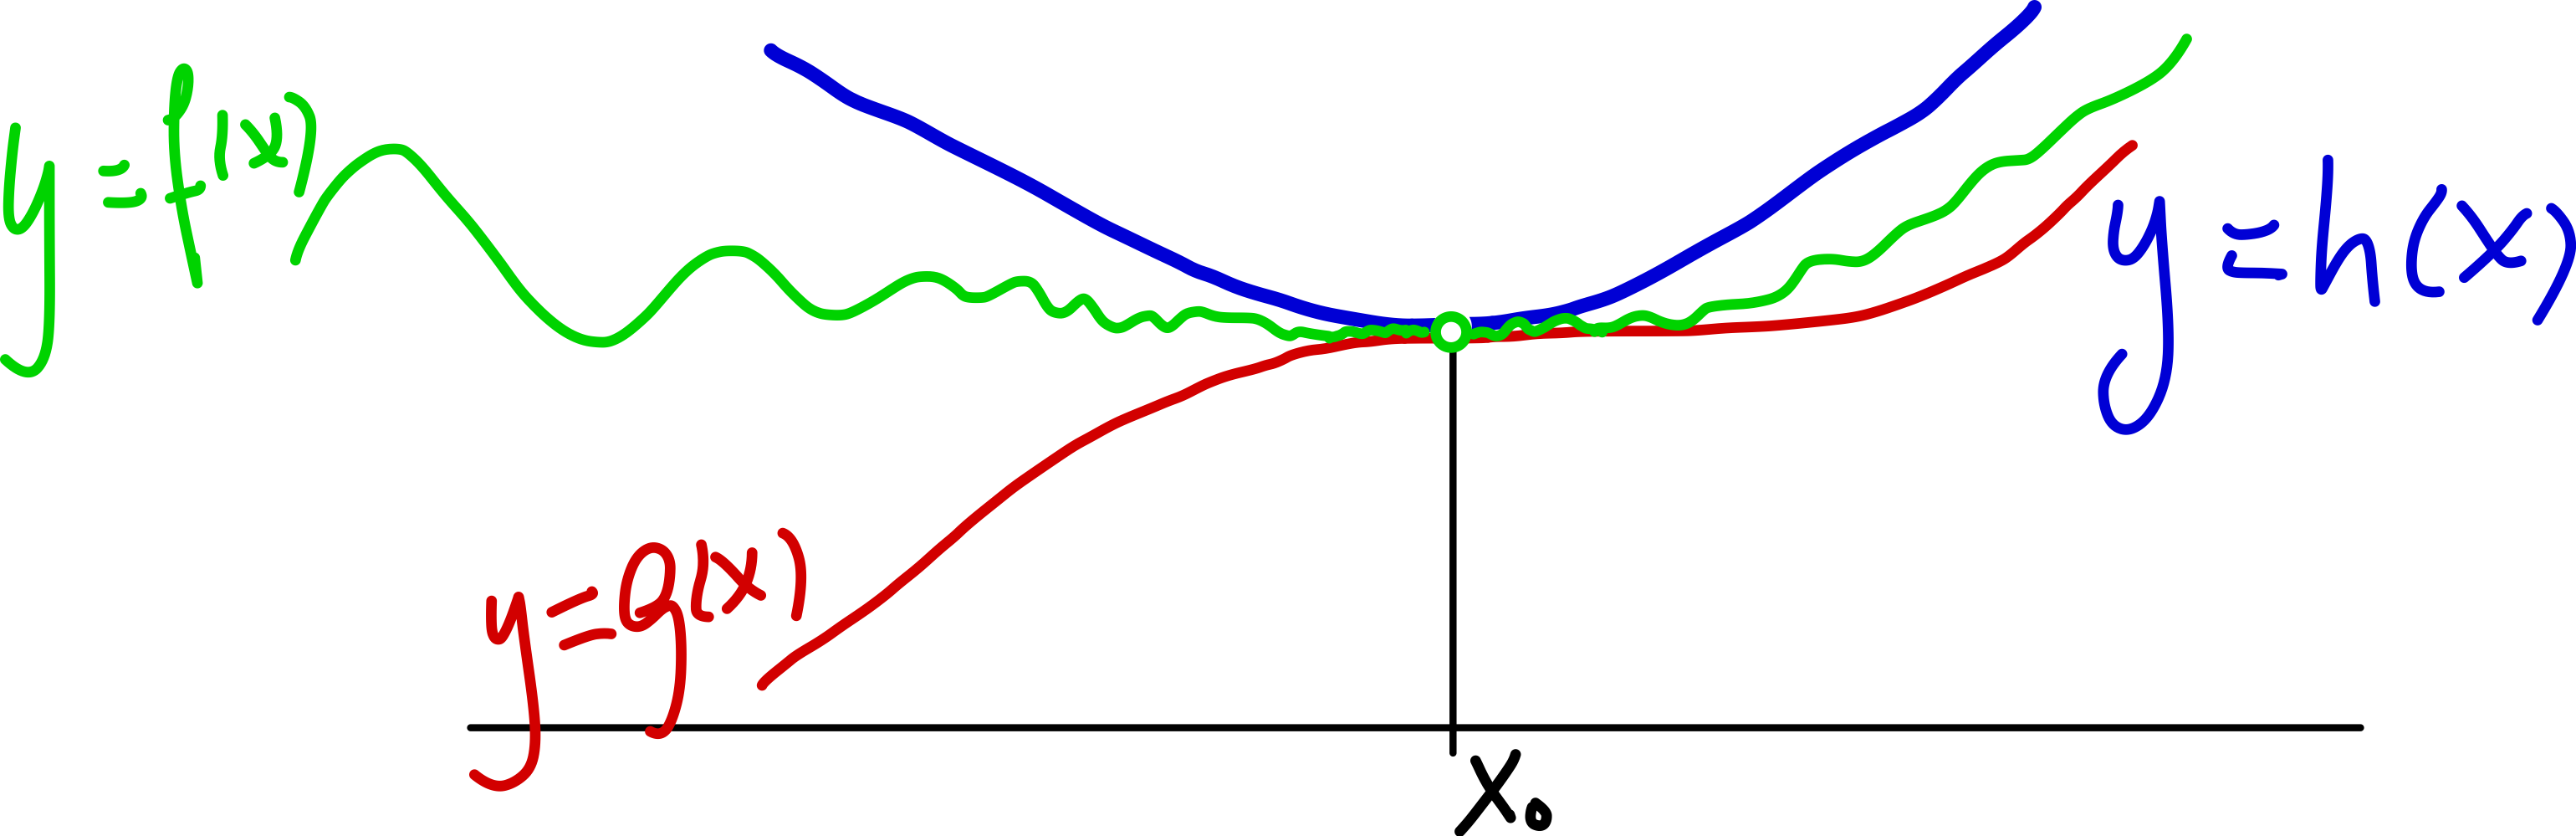
\includegraphics[width=.8\textwidth]{pics/emparedado.png}}


\begin{proposition}
    Sean $f$ y $g$ dos funciones tales que
    \[
    \lim_{x\to x_0} f(x)=\ell_1,
    \qquad
    \lim_{x\to x_0} g(x)=\ell_2.
    \]
    Entonces
    \begin{itemize}
        \item $\D \lim_{x\to x_0} \big( f(x) + g(x) \big) = \ell_1 + \ell_2$;
        \item $\D \lim_{x\to x_0} \big( f(x) \cdot g(x) \big) = \ell_1 \cdot \ell_2$;
        \item Si $\ell_2\neq 0$, $\D \lim_{x\to x_0} \frac{f(x)}{g(x)} = \frac{\ell_1}{\ell_2}$.
    \end{itemize}
\end{proposition}

\begin{example}
    Con estas nuevas reglas de cálculo, sabiendo que\footnote{Estos dos límites están para ser demostrados en los ejercicios.}
    \begin{itemize}
        \item $\D\lim_{x\to x_0} c=c$, para cualquier constante $c$.
        \item $\D\lim_{x\to x_0} x = x_0$, para cualquier $x_0\in\R$.
    \end{itemize}
    podemos ver que:
    \begin{itemize}
        \item $\D\lim_{x\to -1}  \big(3x+x^2\big) = -2$. En efecto
        \[ \lim_{x\to -1} 3x+ \lim_{x\to -1} x^2= 
        \lim_{x\to -1} 3 \cdot \lim_{x\to -1}x+ \lim_{x\to -1} x \cdot \lim_{x\to -1} x= 3\cdot(-1)+(-1)\cdot(-1)=-2.\]
        \item $\D\lim_{x\to 0} \frac{2x+1}{10+x^2}  = \frac{\lim_{x\to 0}(2x+1)}{\lim_{x\to 0}(10+x^2)}=\frac1{10}$ (porque el límite del denominador es no nulo).
        \item Si $p$ y $q$ son polinomios, entonces
        \[ 
        \D\lim_{x\to 1}  \frac{p(x)}{q(x)}  = \frac{\lim_{x\to 1}p(x)}{\lim_{x\to 1}q(x)} 
        =\frac{p(1)}{q(1)},\quad\text{si $q(1)\neq 0$.}
        \]
        
    \end{itemize}
\end{example}

\subsection{Más propiedades del límite}

\begin{theorem}[Teorema fundamental del límite]\label{T:TFL}
Sea $f$ una función definida en $(a,b)$ salvo quizás en $x_0\in(a,b)$.
Entonces 
\[ \D \limxo f(x)=\ell
\]
si y sólo si 
\begin{quote}
    para toda sucesión $\big(x_n\big)_{n\in\N}$ tal que $\D\lim_{n\to\infty} x_n = x_0$ (con $x_n\neq x_0$, para todo \niN) vale que $\lim_{n\to\infty}f(x_n)=\ell$.
\end{quote}
\end{theorem}

\begin{proof}
Supongamos primero que $\limxo f(x)=\ell$ y sea $\big(x_n\big)_{n\in\N}$ una sucesión tal que $\D\lim_{n\to\infty} x_n = x_0$ (con $x_n\neq x_0$, para todo \niN).
Sea $\epsilon>0$, entonces, como $\limxo f(x)=\ell$ existe $\delta>0$ tal que
\[
0<|x-x_0|<\delta\quad\implies\quad |f(x)-\ell|<\epsilon.
\]
Ahora bien, como $\D\lim_{n\to\infty} x_n = x_0$, para ese $\delta>0$, existe $N_0\in\N$ tal que
\[
|x_n-x_0|<\delta, \quad\text{para todo $n\ge N_0$}.
\]
Como además $x_n\neq x_0$, para todo \niN, resulta que 
\[
0<|x_n-x_0|<\delta, \quad\text{para todo $n\ge N_0$}.
\]
Luego, $\D |f(x_n)-\ell|<\epsilon, \quad\text{para todo $n\ge N_0$}$.

Hemos probado que dado $\epsilon>0$ existe $N_0\in\N$ tal que 
\[
|f(x_n)-\ell|<\epsilon, \quad\text{para todo $n\ge N_0$}.
\]
Es decir, $\D\lim_{n\to\infty}f(x_n) = \ell$.

Para probar la recíproca, supongamos que para toda sucesión $\big(x_n\big)_{n\in\N}$ tal que $\D\lim_{n\to\infty} x_n = x_0$ (con $x_n\neq x_0$, para todo \niN) vale que $\lim_{n\to\infty}f(x_n)=\ell$.
Debemos probar que $\D\limxo f(x)=\ell$.
Si esto no fuera cierto, entonces existiría $\epsilon>0$ tal que, cualquiera sea $\delta>0$, hay un $x$ que cumple $0<|x-x_0|<\delta$ y $|f(x)-\ell|\ge \epsilon$.
Entonces, tomamos, para cada $n\in\N$, $\delta=\frac1n$ y sea $x_n$ el correspondiente que cumple que $0<|x_n-x_0|<\frac1n$ y $|f(x_n)-\ell|\ge \epsilon$.
De esta manera, hemos construido una sucesión $\big(x_n\big)_{n\in\N}$ tal que $\D\lim_{n\to\infty} x_n = x_0$, con $x_n\neq x_0$, para todo \niN, para la cual no es cierto que $\lim_{n\to\infty}f(x_n)=\ell$. Esto contradice nuestra suposición, por lo que $\D\limxo f(x)=\ell$.
\end{proof}


\begin{example}
Con este teorema podemos conocer muchos más límites, por ejemplo:
\begin{itemize}
\item ?`$\D \lim_{x\to 25} \sqrt{x} $?
Veamos, si $\sucxn$ es una sucesión tal que $\lim_{n\to\infty} x_n = 25$, entonces $\D \lim_{n\to\infty} \sqrt{x_n} = \sqrt{25}=5$ por lo que hemos visto en el Capítulo~\ref{C:sucesiones}. Como esto se cumple para toda sucesión con límite igual a $25$, resulta que $\D \lim_{x\to 25} \sqrt{x} = 5$.
\end{itemize}
    
\end{example}

Este último teorema, más el trabajo hecho en el Capítulo~\ref{C:sucesiones} nos permite deducir en forma sencilla otras propiedades del límite:

\begin{proposition}
% Sean $f$ y $g$ funciones definidas en $(a,b)$ salvo quizás en $x_0\in(a,b)$.
Si se cumple que
\[
\limxo f(x)=\ell_1>0,
\qquad
\limxo g(x)=\ell_2,
\]
entonces
\begin{enumerate}[{\bf (a)}]
    \item $\D \limxo \big( \ln(f(x)) \big) = \ln (\ell_1)$.
    \item $\D \limxo f(x)^{g(x)} = \ell_1^{\ell_2}$.
\end{enumerate}
\end{proposition}

\begin{proof}
\begin{enumerate}[{\bf (a)}]
    \item Sea \sucxn una sucesión que tiende a $x_0$ ($x_n\neq x_0$, $\forall \niN$),
    entonces $f(x_n)$ tiende a $\ell_1$ por el Teorema~\ref{T:TFL}. 
    Luego, por la Proposición~\ref{P:logaritmo continuo}, 
    \[
    \lim_{n\to\infty} \big(\ln (f(x_n))\big) = \ln (\ell_1).
    \]
    Como esta conclusión vale para cualquier sucesión \sucxn que cumple la hipótesis, 
    resulta nuevamente por el Teorema~\ref{T:TFL} que $\D\limxo \big( \ln (f(x)) \big) = \ln (\ell_1)$.
    
    \item Sea \sucxn una sucesión que tiende a $x_0$ ($x_n\neq x_0$, $\forall \niN$),
    entonces $f(x_n)$ tiende a $\ell_1$ y $g(x_n)$ tiende a $\ell_2$ por el Teorema~\ref{T:TFL}. 
    Luego, por la Proposición~\ref{P:potencias continuas}, 
    \[
    \lim_{n\to\infty} f(x_n)^{g(x_n)} = \ell_1^{\ell_2}.
    \]
    Como esta conclusión vale para cualquier sucesión \sucxn que cumple la hipótesis, 
    resulta nuevamente por el Teorema~\ref{T:TFL} que $\D \limxo f(x)^{g(x)} = \ell_1^{\ell_2}$.\qedhere
\end{enumerate}
\end{proof}


\begin{example}
    Con este teorema podemos ver más ejemplos:
    \begin{itemize}
        \item $\D \lim_{x \to 8} \ln(4x-5) = \ln\big(\lim_{x\to 8} (4x-5)\big)=\ln (4\cdot 8-5) = \ln 27$.
        \item $\D \lim_{x \to 2} \ln \big( 2^{x+1} \big)
        = \ln \big( \lim_{x \to 2}  2^{x+1} \big)
        = \ln \big(   2^{\lim_{x \to 2} x+1} \big)
        = \ln \big(   2^{2+1} \big) = \ln 2^3 = 3 \ln 2
        $.
        \item $\D \lim_{x \to 2} (3x^2)^{4x+1} 
        = \big(\lim_{x \to 2}3x^2\big)^{\lim_{x \to 2}4x+1} 
        = (3\cdot2^2)^{4\cdot 2 + 1 }
        = 12^{9}
        $.
        \item $\D \lim_{x \to -3} \big(x^2+1\big)^x
        = \big(\lim_{x \to -3}x^2+1\big)^{\lim_{x \to -3}x}
        = \big((-3)^2+1\big)^{-3}
        = 10^{-3} = 0.001
        $.
    \end{itemize}
\end{example}


\begin{proposition}
    Sea $g$ una función %definida en $(a,b)$ salvo quizás en $x_0\in(a,b)$, y 
    tal que
    \[
    \limxo g(x) = y_0.
    \]
    Supongamos que $\lim_{y\to y_0}f(y)=f(y_0)$ (el límite de $f(y)$ cuando $y\to y_0$ existe y coincide con $f(y_0)$), entonces
    \[
    \limxo f\circ g(x) = f(y_0) = f(\limxo g(x)).
    \]
\end{proposition}

\begin{proof}
Sea \sucxn una sucesión que tiende a $x_0$ ($x_n\neq x_0$, $\forall \niN$), entonces 
\[
\lim_{n\to\infty} g(x_n) = y_0.
\]
Por lo tanto, la sucesión \sucyn dada por $y_n=g(x_n)$ es una sucesión que cumple $\D\lim_{n\to\infty}y_n=y_0$, 
y por el Teorema~\ref{T:TFL} resulta que $\D\lim_{n\to\infty}f(y_n)=f(y_0)$. Es decir
\[
\lim_{n\to\infty}f\circ g(x_n) = \lim_{n\to\infty}f(y_n)=f(y_0).
\]
Nuevamente, por el Teorema~\ref{T:TFL} resulta que $\D\limxo f\circ g(x) = f(y_0)$.
\end{proof}

\begin{example}
    Con este teorema podemos ver más ejemplos:
    \begin{itemize}
        \item $\D \lim_{x\to 4} \sgn(\underbrace{1-x}_{y})
        = \lim_{y\to -3} \sgn(y)=-1
        $,
        porque $\lim_{x\to4}y = -3$.
        \item $\D \lim_{x\to 0} \big(\underbrace{3x^2+8x+6}_{y\tox{0}6}\big)^7
        =\lim_{y\to 6} y^7 = 6^7
        $.
        \item $\D \lim_{x\to -1} \big(\underbrace{x+2}_{y\tox{-1}1}\big)^{1/5} 
        =\lim_{y\to 1} y^{1/5}=1^{1/5}=1
        $.
        \item $\D \lim_{x\to 3} \bigg[\ln\Big(\underbrace{\frac{x^2+3}{x-1}}_{y\tox{3}6}\Big)\bigg]^4
        =\lim_{y\to 6} \big[\underbrace{ \ln y}_{z\toy{6} \ln 6} ]^4
        = [\ln 6]^4
        $.
    \end{itemize}
\end{example}

\subsubsection*{Ejercicios de la sección~\getcurrentref{chapter}.\getcurrentref{section}}

\begin{enumerate}
\item Probar usando la definición que se cumplen las siguientes afirmaciones:

\begin{multicols}{2}
    \begin{enumerate}
        \item $\D \lim_{x\to 2} 3x-1=5 $.
        \item $\D \lim_{x\to 3} 4 x^2 = 36$.
        \item $\D \lim_{x\to 2} 3/x = 3/2$.
        \item $\D \lim_{x\to 1} x^2+2x = 3$.
    \end{enumerate}
\end{multicols}

\item Analizar la existencia de los siguientes límites:
\begin{multicols}{2}
    \begin{enumerate}
\item $\D \lim_{x\to 0} \sen \frac1x$;
\item $\D \lim_{x\to 0} \cos \frac1x$;
\item $\D \lim_{x\to 0} \sgn(x)$;
\item $\D \lim_{x\to 0} x \sen \frac1x$;
\item $\D \lim_{x\to 0} x^2 \sen \frac1x$;
\item $\D \lim_{x\to 0} (x + \sen \frac1x)$.
\end{enumerate}
\end{multicols}

\item ?`Para qué valores de $x_0\in\R$ existe $\limxo \lfloor x \rfloor$?

\item ?`Para qué valores de $x_0\in\R$ existe $\limxo \big(x - \lfloor x \rfloor\big)$?

\item Analizar la veracidad o falsedad de las siguientes afirmaciones:
\begin{enumerate}
    \item Si existe $\D\limxo \big(f(x)+g(x)\big)$, entonces existen
    $\D\limxo f(x)$ y $\D\limxo g(x)$.
    \item Si existe $\D\limxo \big(f(x)+g(x)\big)$ y existe
    $\D\limxo f(x)$, entonces existe $\D\limxo g(x)$.
    \item Si existe $\D\limxo \big(f(x)\cdot g(x)\big)$, entonces existen
    $\D\limxo f(x)$ y $\D\limxo g(x)$.
    \item Si existe $\D\limxo \big(f(x)\cdot g(x)\big)$ y existe
    $\D\limxo f(x)$, entonces existe $\D\limxo g(x)$.
    \item Si existe $\D\limxo \big(f(x)\cdot g(x)\big)$ y existe
    $\D\limxo f(x)\neq 0$, entonces existe $\D\limxo g(x)$.
    
\end{enumerate}

\item Sea $a>0$, $a\neq 1$ y supongamos que $\limxo f(x)=\ell>0$.
Demostrar que $\D\limxo \log_a(f(x)) = \log_a(\ell).$ (Recordar que $\D\log_a y = \frac{\ln y}{\ln a}$).

\item Consideremos la función constante $f(x)=a$, para algún $a\in\R$. Demostrar usando la definición que $\limxo f(x)=f(x_0)$, cualquiera sea $x_0\in\R$.
\item Consideremos la función \emph{identidad} $f(x)=x$. Demostrar usando la definición que $\limxo f(x)=f(x_0)$, cualquiera sea $x_0\in\R$.
\item Demostrar que si $a$ y $b$ son números reales, entonces la función lineal $f(x)=ax+b$ cumple que $\limxo f(x)=f(x_0)$, cualquiera sea $x_0\in\R$.
Usar lo demostrado en los ejercicios anteriores y las propiedades vistas en esta sección.
\item Demostrar que si $a$, $b$ y $c$ son números reales, entonces la función cuadrática $f(x)=ax^2+bx+c$ cumple que $\limxo f(x)=f(x_0)$, cualquiera sea $x_0\in\R$.
Usar lo demostrado en los ejercicios anteriores y las propiedades vistas en esta sección.
\item Demostrar que si $p(x)$ es una función polinomial, entonces $\limxo p(x)=p(x_0)$, cualquiera sea $x_0\in\R$.
\item Demostrar que si $p(x)$ y $q(x)$ son funciones polinomiales, entonces para la función racional $f(x)= \frac{p(x)}{q(x)}$ se cumple que $\limxo f(x)=f(x_0)$, cualquiera sea $x_0\in\R$, si $q(x_0)\neq0$.


\end{enumerate}


\section{Límites infinitos}

Ampliamos ahora el estudio del límite, considerando la posibilidad de que la variable $x$, o la función $f(x)$, o ambas, crezcan más allá de todo límite.

Comenzamos definiendo límites infinitos cuando $x$ tiende a un número real $x_0$.

\begin{definition}
    Sea $f$ una función definida en $(x_0,x_0+c)$ para algún $c>0$.
    Decimos que $f(x)$ tiende a $+\infty$ cuando $x$ tiende a $x_0$ por derecha, y escribimos
    \[
    \limxop f(x)=+\infty
    \]
    si se cumple lo siguiente:
    \begin{quote}
        Cualquiera sea $M>0$ existe $\delta>0$ tal que
        \[
        f(x)>M,\quad\text{para todo $x\in(x_0,x_0+\delta)$}.
        \]
    \end{quote}
\end{definition}

\begin{example}
    Veamos que 
    \[
    \lim_{x\to0^+} \frac1x = +\infty.
    \]
    Sea $M>0$, vemos que $\frac1x>M$ si y sólo si $0<x<\frac1M$. Por lo tanto, elegimos $\delta=\frac1M$ y se cumple que $\frac1x>M$ para todo $x\in(0,\delta)$.

    Hemos demostrado que dado $M>0$ existe $\delta>0$ tal que $\frac1x>M$ para todo $x\in(0,\delta)$.
    Luego $\D \lim_{x\to0^+} \frac1x = +\infty$.
\end{example}

Análogamente se define el límite infinito por izquierda.

\begin{definition}
    Sea $f$ una función definida en $(x_0-c,x_0)$ para algún $c>0$.
    Decimos que $f(x)$ tiende a $+\infty$ cuando $x$ tiende a $x_0$ por izquierda, y escribimos
    \[
    \limxom f(x)=+\infty
    \]
    si se cumple lo siguiente:
    \begin{quote}
        Cualquiera sea $M>0$ existe $\delta>0$ tal que
        \[
        f(x)>M,\quad\text{para todo $x\in(x_0-\delta,x_0)$}.
        \]
    \end{quote}
\end{definition}

\begin{example}
    Veamos que 
    \[
    \lim_{x\to0^-} \frac1{x^2} = +\infty.
    \]

    Sea $M>0$, vemos que $\frac1{x^2}>M$ si y sólo si $0<x^2<\frac1M$, o $\frac1M<\frac{1}{x^2}$. Por lo tanto, elegimos $\delta=\sqrt{\frac1M}$ y se cumple que $\frac1{x^2}>M$ para todo $x\in(-\delta,0)$.

    Hemos demostrado que dado $M>0$ existe $\delta>0$ tal que $\frac1{x^2}>M$ para todo $x\in(-\delta,0)$.
    Luego $\D \lim_{x\to0^-} \frac1{x^2} = +\infty$.
\end{example}

Ahora definimos los otros límites infinitos, como lo hicimos con sucesiones.

\begin{definition}
\begin{itemize}
    \item $\D\limxop f(x) = -\infty$ significa $\D\limxop \big(-f(x)\big)=+\infty$.
    \item $\D\limxom f(x) = -\infty$ significa $\D\limxom \big(-f(x)\big)=+\infty$.
    \item $\D\limxop f(x) = \infty$ significa $\D\limxop \big|f(x)\big|=+\infty$.
    \item $\D\limxom f(x) = \infty$ significa $\D\limxom \big|f(x)\big|=+\infty$.
\end{itemize}
\end{definition}

\begin{example}
    Veamos un ejemplo. Afirmamos que
    \[
    \lim_{x\to 0^+} \ln x = -\infty.
    \]
    Esto significa que $\lim_{x\to 0^+} \big(-\ln x\big) = +\infty$. Es decir, dado $M>0$ existe $\delta>0$ tal que vale la siguiente implicación
    \[
    0<x<\delta \quad\implies\quad -\ln x > M.
    \]
    Sea entonces $M>0$, consideremos $\delta = e^{-M}$. Si $0<x<\delta$, como $\ln$ es creciente, entonces $\ln x<\ln \delta = \ln e^{-M} = -M$, por lo tanto
    \[
    -\ln x > M.
    \]
    Hemos demostrado que dado $M>0$ existe $\delta>0$ tal que $-\ln x > M$ para todo $x\in (0,\delta)$. Es decir, $\lim_{x\to 0^+} \big(-\ln x\big) = +\infty$ que equivale a $\lim_{x\to 0^+}\ln x=-\infty$.
\end{example}

Nos falta considerar el caso en que la variable $x$ tiende a infinito.

\begin{definition}
    Sea $f$ definida en todos los puntos de un intervalo $(a,+\infty)$. Entonces
    \begin{itemize}
        \item Se dice que $\D\lim_{x\to +\infty} f(x) = \ell$ si, dado $\epsilon>0$ existe $K>0$ tal que 
        \[
        |f(x)-\ell|<\epsilon,
        \qquad\text{para todo $x>K$}.
        \]
        \item Se dice que $\D\lim_{x\to +\infty} f(x) = +\infty$ si, dado $M>0$ existe $K>0$ tal que 
        \[
        f(x)>M,
        \qquad\text{para todo $x>K$}.
        \]
        \item $\D\lim_{x\to +\infty} f(x) = -\infty$ significa que $\D\lim_{x\to +\infty}\big(- f(x)\big) = +\infty$
        \item $\D\lim_{x\to +\infty} f(x) = \infty$ significa que $\D\lim_{x\to +\infty}\big|f(x)\big| = +\infty$
    \end{itemize}
\end{definition}


\begin{example}
    Veamos que, si $\alpha>0$
    \[
    \lim_{x\to+\infty} x^{-\alpha} = 0.
    \]
    Sea $\epsilon>0$, observamos que para $x>0$, resulta
    \[
    0<x^{-\alpha}<\epsilon
    \quad\iff\quad
    0<\frac{1}{x^{\alpha}}<\epsilon
    \quad\iff\quad
    \frac1\epsilon<x^\alpha
    \quad\iff\quad
    \frac1{\epsilon^{1/\alpha}}<x.
    \]
    Elegimos entonces $K=1/{\epsilon^{1/\alpha}}$ y llegamos a que
    \[
    0< x^{-\alpha } < \epsilon, \qquad\text{para todo $x>K$},
    \]
    que a su vez implica que
    \[
    |x^{-\alpha } - 0| < \epsilon, \qquad\text{para todo $x>K$},
    \]
    Como $\epsilon>0$ era arbitrario, resulta que $\D\lim_{x\to+\infty} x^{-\alpha} = 0$.
\end{example}


\begin{example}
    Veamos que, si $\alpha>0$
    \[
    \lim_{x\to+\infty} x^{\alpha} = +\infty.
    \]
    Sea $M>0$, observamos que 
    \[
    x^\alpha > M
    \quad\iff\quad
    x > M^{1/\alpha}.
    \]
    Luego, elegimos $K = M^{1/\alpha}$ y resulta que 
    \[
    x^{-\alpha } > M, \qquad\text{para todo $x>K$}.
    \]
    Como $M>0$ era arbitrario, resulta que $\D\lim_{x\to+\infty} x^{\alpha} = +\infty$.
\end{example}

\begin{example}
    Veamos un ejemplo más. Afirmamos que 
    \[
    \lim_{x\to+\infty} \ln x = +\infty.
    \]
    Sea $M>0$, tomemos $K=e^M$, entonces, como la función $\ln$ es estrictamente creciente, resulta que, si $x>K$
    \[
    \ln x > \ln K = \ln e^M = M.
    \]
    Hemos demostrado que dado $M>0$ existe $K>0$ tal que 
    \[
    \ln x > M, 
        \qquad\text{para todo $x>K$}.
    \]
    Es decir, $\D\lim_{x\to+\infty} \ln x = +\infty$.
\end{example}

\begin{example}
    Consideremos ahora la función exponencial. Afirmamos que si $a>1$ entonces
    \[
    \lim_{x\to+\infty} a^x = +\infty.
    \]
    Sea $M>0$, tomemos $K=\max\{\log_a M, 1\}$ (si $M<1$ resulta $\log_a M<0$). Como $a>1$, la función $x\to a^x$ es estrictamente creciente, y entonces, si $x>K$ resulta que,
    \[
    a^x > a^K \ge a^{\log_a K} = K.
    \]
    Hemos demostrado que dado $M>0$ existe $K>0$ tal que 
    \[
    a^x > M, 
        \qquad\text{para todo $x>K$}.
    \]
    Es decir, $\lim_{x\to+\infty} a^x = +\infty$.
\end{example}

Presentamos ahora las últimas definiciones de límites cuando la variable independiente $x$ tiende a infinito.
\begin{definition}
    Sea $f$ definida en todos los puntos de un intervalo $(-\infty,a)$. Entonces
    \begin{itemize}
        \item Se dice que $\D\lim_{x\to -\infty} f(x) = \ell$ si, dado $\epsilon>0$ existe $K>0$ tal que 
        \[
        |f(x)-\ell|<\epsilon,
        \qquad\text{para todo $x<-K$}.
        \]
        \item Se dice que $\D\lim_{x\to -\infty} f(x) = +\infty$ si, dado $M>0$ existe $K>0$ tal que 
        \[
        f(x)>M,
        \qquad\text{para todo $x<-K$}.
        \]
        \item $\D\lim_{x\to -\infty} f(x) = -\infty$ significa que $\D\lim_{x\to -\infty}\big(- f(x)\big) = +\infty$
        \item $\D\lim_{x\to -\infty} f(x) = \infty$ significa que $\D\lim_{x\to -\infty}\big|f(x)\big| = +\infty$
    \end{itemize}
\end{definition}

\begin{example}
    Veamos que, si $n\in\N$
    \[
    \lim_{x\to-\infty} x^{-n} = 0.
    \]
    Sea $\epsilon>0$, observamos que para $x<0$, resulta
    \[
    |x^{-n}-0|<\epsilon
    \quad\iff\quad
    0<\frac{1}{|x|^n}<\epsilon
    \quad\iff\quad
    \frac1\epsilon<|x|^n
    \quad\iff\quad
    \frac1{\epsilon^{1/n}}<|x|.
    \]
    Elegimos entonces $K=1/{\epsilon^{1/n}}$ y llegamos a que
    \[
    | x^{-n} - 0| < \epsilon, 
    \qquad\text{para todo $x<-K$},
    \]
    Como $\epsilon>0$ era arbitrario, resulta que $\D\lim_{x\to-\infty} x^{-n} = 0$.
\end{example}

\begin{example}
    Veamos que, si $n\in\N$
    \[
    \lim_{x\to-\infty} x^{n} = \begin{cases} 
    +\infty, \quad&\text{si $n$ es par,}\\
    -\infty, \quad&\text{si $n$ es impar.}
    \end{cases}
    \]
    Consideremos el caso de $n$ impar.
    Tenemos que ver que $\D\lim_{x\to-\infty} -x^{n} = +\infty$.
    Pero si $n$ es impar $-x^n = (-x)^n$. Para $x<0$ tenemos que $(-x)^n=|x|^n$.
    Ahora bien 
    \[
    (-x)^n > M 
    \quad\iff\quad
    (-x) > M^{1/n}
    \quad\iff\quad
    x < - M^{1/n}.
    \]
    Elegimos $K = M^{1/n}$ y resulta que 
    \[
    (-x)^n > M ,
    \qquad\text{para todo $x<-K$}.
    \]
    Como $K>0$ era arbitrario, resulta que $\D\lim_{x\to-\infty} -x^{n} = +\infty$, o lo que es lo mismo $\D\lim_{x\to-\infty} x^{n} = -\infty.$
\end{example}

\begin{example}
    Consideremos nuevamente la función exponencial. Afirmamos que si $a>1$ entonces
    \[
    \lim_{x\to-\infty} a^x = 0.
    \]
    Sea $\epsilon>0$, tomemos $K=\max\{-\log_a \epsilon, 1\}$ (si $\epsilon>1$ resulta $\log_a \epsilon>0$). Como $a>1$, la función $x\to a^x$ es estrictamente creciente, y entonces, si $x<-K$ resulta que,
    \[
    0< a^x < a^{-K} \le a^{\log_a \epsilon} = \epsilon,
    \]
    que implica
    \[
    |a^x-0| < \epsilon.
    \]
    
    Hemos demostrado que dado $M>0$ existe $K>0$ tal que 
    \[
    |a^x-0| < \epsilon.
        \qquad\text{para todo $x<-K$}.
    \]
    Es decir, $\lim_{x\to-\infty} a^x = 0$.
\end{example}

Para todos los límites que hemos visto se cumplen las propiedades siguientes con demostraciones análogas a las que ya hemos visto:

\begin{itemize}
    \item Si $\D \lim f(x) = \ell_1$ y $\D \lim g(x)=\ell_2$, entonces:
    \begin{itemize}
        \item $\D \lim \big(f(x)+g(x)\big) = \ell_1+\ell_2$.
        \item $\D \lim \big(f(x)\cdot g(x)\big) = \ell_1\cdot \ell_2$.
        \item $\D \lim \big(f(x)/g(x)\big) = \ell_1/\ell_2$, si $\ell_2\neq 0$.
        \item $\D \lim \big(f(x)/g(x)\big) = \infty$, si $\ell_2= 0$ y $\ell_1\neq 0$.
        \item $\D \lim f(x)^{g(x)} = \ell_1^{\ell_2}$, si $\ell_1>0$.
    \end{itemize}
    \item Si $\D \lim f(x) = \ell$ y $\D \lim g(x)=+\infty$, entonces:
    \begin{itemize}
        \item $\D \lim \big(f(x)+g(x)\big) = +\infty$.
        \item $\D \lim \big(f(x)\cdot g(x)\big) = \begin{cases}
            +\infty, \quad&\text{si }\ell>0,\\
            -\infty, \quad&\text{si }\ell<0,\\
            \text{indeterminado}, \quad&\text{si }\ell=0.
        \end{cases}$
        \item $\D \lim \big(f(x)/g(x)\big) = 0$.
        \item $\D \lim f(x)^{g(x)} =\begin{cases}
            +\infty, \quad&\text{si }\ell>1,\\
            0, \quad&\text{si } 0<\ell<1,\\
            0, \quad&\text{si } \ell=0 \text{ y }f(x)\ge 0.
        \end{cases}$
    \end{itemize}
    \item Si $\D \lim f(x) = \ell$ y $\D \lim g(x)=-\infty$, entonces:
    \begin{itemize}
        \item $\D \lim \big(f(x)+g(x)\big) = -\infty$.
        \item $\D \lim \big(f(x)\cdot g(x)\big) = \begin{cases}
            -\infty, \quad&\text{si }\ell>0,\\
            +\infty, \quad&\text{si }\ell<0,\\
            \text{indeterminado}, \quad&\text{si }\ell=0.
        \end{cases}$
        \item $\D \lim \big(f(x)/g(x)\big) = 0$.
        \item $\D \lim f(x)^{g(x)} =\begin{cases}
            0, \quad&\text{si }\ell>1,\\
            +\infty, \quad&\text{si } 0<\ell<1,\\
            +\infty, \quad&\text{si } \ell=0 \text{ y }f(x)\ge 0.
        \end{cases}$
    \end{itemize}
\end{itemize}

\begin{proposition}
    Si $\D\limxo g(x) = +\infty$ y $\D\lim_{y\to+\infty}f(y)=\ell$, entonces $\D\limxo f\circ g(x) = \ell$.
\end{proposition}

\begin{proof}
Sea $\epsilon>0$. Como $\D\lim_{y\to+\infty}f(y)=\ell$, existe $K>0$ tal que
\[
|f(y)-\ell|<\epsilon,
\qquad\text{para todo $y>K$}.
\]
Ahora bien, como $\D\limxo g(x) = +\infty$, existe $\delta>0$ tal que 
\[
0<|x-x_0|<\delta
\quad\implies\quad
g(x) > K.
\]
Por lo tanto, si $0<|x-x_0|<\delta$, resulta
\[
g(x)>K
\quad\implies\quad
|f(g(x))-\ell|<\epsilon
\quad\iff\quad
|f\circ g(x))-\ell|<\epsilon.
\]
Hemos demostrado que dado $\epsilon>0$ existe $\delta>0$ tal que
\[
|f\circ g(x))-\ell|<\epsilon,
\qquad\text{para todo $x\in(x_0-\delta,x_0+\delta)\setminus\{x_0\}$}.
\qedhere
\]
\end{proof}

\begin{example}
    Si definimos $f(y) = \Big(1+\frac1y\Big)^y$, sabemos que $\lim_{y\to+\infty}f(y)=e$.

    Si ahora $g(x)$ es una función que cumple que $\limxo g(x) = +\infty$, entonces
    \[
    \limxo f\circ g(x) = e.
    \]
    Es decir, 
    \[
    \limxo \D \Big(1+\frac{1}{g(x)}\Big)^{g(x)}=e.
    \]

    Lo mismo vale si en todos las fórmulas donde aparece $\limxo$, reemplazamos este límite por $\limxop$, o $\limxom$, o $\lim_{x\to+\infty}$ o $\lim_{x\to-\infty}$.

    Por ejemplo, $\lim_{x\to 0^+}\frac1x=+\infty$, entonces 
    \[
    \lim_{x\to 0^+} \Big(1+\frac{1}{\frac1x}\Big)^{1/x}
    =
    \lim_{x\to 0^+} \Big(1+x\Big)^{1/x} = e.
    \]
    Y también 
    \[
    \lim_{x\to 0^-} \Big(1+x\Big)^{1/x} = e,
    \]
    porque $\lim_{x\to 0^-}\frac1x=-\infty$.

    Por lo tanto, $\D\lim_{x\to 0} \Big(1+x\Big)^{1/x} = e.$
\end{example}

\begin{corollary}
    De manera análoga a la última proposición puede probarse lo siguiente, si $\D\lim_{y\to+\infty}f(y)=\ell$:
    \begin{itemize}
        \item Si $\D\limxop g(x) = +\infty$, entonces $\limxop f\circ g(x) = \ell$
        \item Si $\D\limxom g(x) = +\infty$, entonces $\limxom f\circ g(x) = \ell$
        \item Si $\D\lim_{x\to +\infty} g(x) = +\infty$, entonces $\lim_{x\to +\infty} f\circ g(x) = \ell$
        \item Si $\D\lim_{x\to -\infty} g(x) = +\infty$, entonces $\lim_{x\to -\infty} f\circ g(x) = \ell$
    \end{itemize}
\end{corollary}

\begin{corollary}
    De manera análoga a la última proposición puede probarse lo siguiente, si $\D\lim_{y\to+\infty}f(y)=+\infty$:
    \begin{itemize}
        \item Si $\D\limxop g(x) = +\infty$, entonces $\limxop f\circ g(x) = +\infty$
        \item Si $\D\limxom g(x) = +\infty$, entonces $\limxom f\circ g(x) = +\infty$
        \item Si $\D\lim_{x\to +\infty} g(x) = +\infty$, entonces $\lim_{x\to +\infty} f\circ g(x) = +\infty$
        \item Si $\D\lim_{x\to -\infty} g(x) = +\infty$, entonces $\lim_{x\to -\infty} f\circ g(x) = +\infty$
    \end{itemize}
\end{corollary}

\subsubsection*{Ejercicios de la sección~\getcurrentref{chapter}.\getcurrentref{section}}

\begin{enumerate}
\item Calcular los siguientes límites.
 Si el límite es infinito, indicar si es $+\infty$, $-\infty$ o meramente $\infty$.
   
\begin{multicols}{2}
    \begin{enumerate}
        \item $\D\lim_{x\to0} \frac{1}{x+x^2}$
        \item $\D\lim_{x\to0} \frac{1}{x^2+x^4}$
        \item $\D\lim_{x\to0} \frac{-1}{|x|}$
        \item $\D\lim_{x\to0^+} \frac{1}{\sqrt x}$
        \item $\D\lim_{x\to2} \frac{3}{(x-2)^2}$
        \item $\D\lim_{x\to0} \frac{x}{\sqrt{x^2+1}-1}$
    \end{enumerate}
\end{multicols}

\item Escribir proposiciones que relacionen todas las definiciones de límites de la Sección~\getcurrentref{chapter}.\getcurrentref{section} con límites de sucesiones.

\item Analizar la existencia de los siguientes límites:
   
\begin{multicols}{2}
    \begin{enumerate}
        \item $\D\lim_{x\to+\infty} \sen(x)$
        \item $\D\lim_{x\to+\infty} \cos(x)$
        \item $\D\lim_{x\to+\infty} \frac{\sen(x)}x$
        \item $\D\lim_{x\to+\infty} x\sen\Big(\frac\pi x\Big)$
        \item $\D\lim_{x\to0} \frac{|x|-x}{|x|+x}$
        \item $\D\lim_{x\to0} x\cdot\lfloor x \rfloor$
        \item $\D\lim_{x\to0} x\cdot\bigg\lfloor \frac1x \bigg\rfloor$
    \end{enumerate}
\end{multicols}

\item Calcular los siguientes límites.
 Si el límite es infinito, indicar si es $+\infty$, $-\infty$ o meramente $\infty$.
   
\begin{multicols}{2}
    \begin{enumerate}
    \item $\D \lim_{x\to+\infty} \frac{x^3+2x-1}{2x^3-3x+4}$
    \item $\D \lim_{x\to-\infty} \frac{x^3+2x-1}{2x^3-3x+4}$
    \item $\D \lim_{x\to+\infty} \frac{2x^2-3x}{x^3+1}$
    \item $\D \lim_{x\to-\infty} \frac{2x^2-3x}{x^3+1}$
    \item $\D \lim_{x\to+\infty} \frac{\sqrt{x^2+x+1}+\sqrt{x^2-x+1}}{x+\sqrt{x^2+1}}$
    \item $\D \lim_{x\to-\infty} \frac{\sqrt{x^2+x+1}+\sqrt{x^2-x+1}}{x+\sqrt{x^2+1}}$
    \item $\D \lim_{x\to+\infty} \frac{2+x^{5/3}}{3x+x^{1/5}}$
    \item $\D \lim_{x\to-\infty} \frac{2+x^{5/3}}{3x+x^{1/5}}$
    \item $\D \lim_{x\to+\infty} \frac{\sqrt{x}+x^{3/4}}{x^{1/3}+x^{2/3}}$
    \item $\D \lim_{x\to-\infty} \frac{x^2-1}{x+2}-\frac{x^2+1}{x+2}$
    \item $\D \lim_{x\to+\infty} \frac{\sqrt{x+1}-\sqrt{x-1}}{\sqrt{x+1}+\sqrt{x-1}}$
    \item $\D \lim_{x\to+\infty} x^2-2x$
    \item $\D \lim_{x\to+\infty} 2x^2+6x$
    \item $\D \lim_{x\to+\infty} \frac{\sqrt{x+\sqrt{x}}}{\sqrt{x+\sqrt{x+\sqrt{x}}}}$
    \item $\D \lim_{x\to+\infty} x\big(x-\sqrt{2x^2+3}\big)$
    \item $\D \lim_{x\to+\infty} \sqrt{x^2+2x}-x$
    \item $\D \lim_{x\to+\infty} x+\sqrt{1-x^3}$
    \item $\D \lim_{x\to+\infty} \bigg(\frac{x+1}{x+2}\bigg)^{2x}$
    \item $\D \lim_{x\to+\infty} \bigg(\frac{2x^2+5}{x^2+1}\bigg)^{3x^2+1}$
    \item $\D \lim_{x\to+\infty} \bigg(\frac{x+4}{x+6}\bigg)^{x^2}$
    \item $\D \lim_{x\to+\infty} \bigg(\frac{x^2+1}{x^2+2}\bigg)^{x^3}$
    
    
    \end{enumerate}
\end{multicols}


\end{enumerate}


\section{La notación \texorpdfstring{$o(h)$}{o(h)}}

\begin{definition}
    Sea $f$ una función real definida en $(-c,c)$, salvo quizás en $x=0$, para algún $c>0$. Se dice que $f(h)$ es una \emph{$o$ (chiquita) de $h$ cuando $h$ tiende a cero} y se escribe $f(h)=o(h)$ si
    \[
    \lim_{h\to 0} \frac{f(h)}{h} = 0.
    \]
    Es decir, $f(h) = o(h)$ si \emph{$f(h)$ tiende a cero más rápido que $h$}, cuando $h$ tiende a cero.
\end{definition}

Antes de ver algunos ejemplos, observemos que:
\[
\lim_{h\to 0} \frac{f(h)}{h} = 0
\quad\iff\quad
\lim_{h\to 0} \frac{|f(h)|}{|h|} = 0.
\]

\begin{example} Veamos algunos ejemplos:
\begin{itemize}
    \item Si $f(x) = x^2$, entonces $f(h) = o(h)$.
    En efecto, para $h\neq 0$
    \[
    \frac{f(h)}h = \frac{h^2}{h} = h \to 0 \quad\text{cuando $h\to0$}.
    \]
    % \item Si $f(x) = x^3$, entonces $f(h) = o(h)$.
    \item Si $f(x) = |x|^{1.1}$, entonces $f(h) = o(h)$.
    En efecto, para $h\neq 0$
    \[
    \frac{|f(h)|}{|h|} = \frac{|h|^{1.1}}{|h|} = |h|^{0.1} \to 0 \quad\text{cuando $h\to0$}.
    \]
    % \item Si $f(x) = |x|^\alpha$ y $\alpha > 1$, entonces $f(h) = o(h)$.
    % \item Si $f(x) = \frac{x}{\log x}$, entonces $f(h) = o(h)$.
    % \item Si $f(x) = 1-\cos(x)$, entonces $f(h) = o(h)$.
    % \item Si $f(x) = |x|$, entonces $f(h) \neq o(h)$.
    \item Si $f(x) = \sqrt{|x|}$, entonces $f(h) \neq o(h)$.
    En efecto, para $h\neq 0$
    \[
     \frac{|f(h)|}{|h|} = \frac{\sqrt{|h|}}{|h|} = \frac1{\sqrt{|h|}} \not\to 0 \quad\text{cuando $h\to0$}.
    \]
    % \item Si $f(x) = 1$, entonces $f(h) \neq o(h)$.
    % \item Si $f(x) = |x|^\alpha$ y $\alpha \le 1$, entonces $f(h) \neq o(h)$.
    % \item Si $f(x) = \log(|x|)$, entonces $f(h) \neq o(h)$.
    % \item Si $f(x) = \sen(x)$, entonces $f(h) \neq o(h)$.
\end{itemize}
\end{example}

\begin{lemma}
  Si $f(h)=o(h)$, entonces $\lim_{h\to0}f(h) = 0$.
\end{lemma}

\begin{proof}
    Observamos que, para $h\neq 0$,
    \[
    f(h) = \frac{f(h)}{h} \cdot h .
    \]
    Como $f(h)=o(h)$ resulta que $\lim_{h\to0} \frac{f(h)}{h} = 0$, y obviamente $\lim_{h\to0}h=0$.
    Por lo tanto, por la regla del límite del producto, $\lim_{h\to0}f(h)=0$.
\end{proof}

\begin{remark}
    No es cierto que si $\lim_{h\to0}f(h) = 0$, entonces $f(h) = o(h)$.
    Por ejemplo, la función $f(x) = x$ cumple que $\lim_{h\to0}f(h) = 0$ y sin embargo, $f(h) \neq o(h)$, porque
    \[
    \frac{f(h)}{h} = \frac hh = 1 \not\to 0, \text{ cuando $h\to 0$}.
    \]
\end{remark}


Es fácil deducir las siguientes propiedades.

\begin{theorem}[Propiedades]
    \begin{enumerate}[{\bf(a)}]
        \item Si $f(h)=o(h)$, entonces $cf(h) = o(h)$.
        \item Si $f(h)=o(h)$ y $g(h) = o(h)$, entonces $f(h)+g(h) = o(h)$.
        \item Si $f(h)=o(h)$ y $g(h) = o(h)$, entonces $f(h)g(h) = o(h)$.
    \end{enumerate}
\end{theorem}


\begin{theorem}
Si $f(h)=o(h)$, $f(0)=0$, y $g$ es una función real que cumple
$|g(h)| \le C|h|$, para todo $|h|<p$, para algún $p>0$ y $C>0$, entonces $f\circ g(h) = o(h)$.
\end{theorem}

\begin{proof}
    Tenemos que demostrar que $\lim_{h\to0} \frac{f\circ g(h)}{h} = 0$.
    Observemos que
    \[
    \text{Si $h \neq 0$}, \quad
    \frac{f\circ g(h)}{h} = \begin{cases}
        0,\quad&\text{si }g(h) = 0,\\
        \frac{f(g(h))}{g(h)} \frac{g(h)}{h}, \quad&\text{si }g(h) \neq 0.
    \end{cases}
    \]
    Sea ahora $\eps > 0$. Como $f(H)=o(H)$, existe $\eta > 0$ tal que
    \[
    \left| \frac{f(H)}{H} \right| \le \frac{\eps}{C}, \quad\text{para todo } H \in (-\eta,\eta) .
    \]
    Si ahora elegimos $\delta = \min\{\eta,p\}$ resulta que
    \[
    \left| \frac{f\circ g(h)}{h} \right| < \frac{\eps}C = \eps, \quad\text{para todo }h \in (-\delta,\delta).
    \]
    Hemos demostrado que dado $\eps > 0$ existe $\delta > 0$ tal que
    \[
    \left| \frac{f\circ g(h)}{h} - 0 \right| < \eps, \quad\text{para todo }h \in (-\delta,\delta).
    \]
    Es decir, $\lim_{h \to 0} \frac{f\circ g(h)}{h} = 0$, o lo que es lo mismo, $f\circ g(h) = o(h)$.
\end{proof}


\subsubsection*{Ejercicios de la sección~\getcurrentref{chapter}.\getcurrentref{section}}

\begin{enumerate}
\item Determinar cuáles de las siguientes funciones cumplen que $f(h)=o(h)$:
\begin{multicols}{2}
\begin{enumerate}
    % \item $f(x) = x^2$
    \item $f(x) = x^3$
    \item $f(x) = 1$
    \item $f(x) = |x|^{1.001}$
    \item $f(x) = |x|^\alpha$ con $\alpha > 1$
    \item $f(x) = |x|^{1/3}$
    \item $f(x) = |x|$
    \item $f(x) = |x|^\alpha$ con $\alpha \le 1$
    \item $f(x) = \frac{x}{\log |x|}$
    % \item $f(x) = 1-\cos(x)$
    \item $f(x) = \log(|x|)$
    \item $f(x) = e^x$
    \item $f(x) = e^{-1/|x|}$
    
    % \item $f(x) = \sen(x)$, 
\end{enumerate}    
\end{multicols}

\item Demostrar las siguientes afirmaciones:
    \begin{enumerate}
        \item Si $f(h)=o(h)$, entonces $cf(h) = o(h)$.
        \item Si $f(h)=o(h)$ y $g(h) = o(h)$, entonces $f(h)+g(h) = o(h)$.
        \item Si $f(h)=o(h)$ y $g(h) = o(h)$, entonces $f(h)g(h) = o(h)$.
    \end{enumerate}

\end{enumerate}

\section{Funciones continuas}

Vimos en la primera sección de este capítulo (en la Definición~\ref{D:continuidad}) que
una función $f(x)$ es continua en $x_0$ si se cumple lo siguiente:
    \begin{quote}
        Para cada $\epsilon > 0$, existe $\delta > 0$ tal que
        \[ 
        |f(x) - f(x_0)| < \epsilon,
        \]
        para todos los valores $x$ que cumplen $|x-x_0|<\delta$.
    \end{quote}

Luego vimos que $\lim_{x\to x_0} f(x) = \ell$ (Definición~\ref{D:limite}) si se cumple lo siguiente:
    \begin{quote}
        Para cada $\epsilon > 0$, existe $\delta > 0$ tal que
        \[ 
        |f(x) - \ell| < \epsilon,
        \]
        para todos los valores $x$ que cumplen $0<|x-x_0|<\delta$.
    \end{quote}

Analizando estas dos definiciones, vemos que
\[
f \text{ es continua en $x_0$}
\quad\text{si y sólo si}\quad
\limxo f(x) = f(x_0).
\]
Es decir, una función $f$ es continua en un punto $x_0$ si:
\begin{itemize}
    \item Existe (y es finito) $\D\limxo f(x)$;
    \item $f$ está definida en $x_0$, es decir, existe $f(x_0)$;
    \item El límite coincide con el valor de la función en ese punto: $\D\limxo f(x)=f(x_0)$.
\end{itemize}

Entonces hay tres condiciones que implican la \emph{discontinuidad} de una función $f$ en un punto $x_0$:

\begin{enumerate}
    \item Si no existe $\D\limxo f(x)$ (o es infinito).
    \begin{itemize}
        \item Para la función \emph{signo}:
        \[
         f(x) = \sgn(x)  = \begin{cases}
    -1, \quad &\text{si $x<0$},\\
    0, \quad &\text{si $x=0$},\\
    1, \quad &\text{si $x>0$},
    \end{cases}
    \]
    no existe $\lim_{x\to 0} f(x)$, dado que los límites por izquierda y por derecha no coinciden.
    Por lo tanto $f(x)$ no es continua en $x_0=0$.

    \item Para la función
    \[
    f(x) = \begin{cases}
    \sen\frac1x, \quad &\text{si $x\neq0$},\\
    0, \quad &\text{si $x=0$},
    \end{cases}
    \]
    tampoco existe $\lim_{x\to 0} f(x)$ (ya vimos esto en un ejercicio).
    Por lo tanto $f(x)$ no es continua en $x_0=0$.

    \item Para la función 
    \[
    f(x) = \begin{cases}
    \frac1x, \quad &\text{si $x\neq0$},\\
    0, \quad &\text{si $x=0$},
    \end{cases}
    \]
    se cumple que $\lim_{x\to0}f(x) = \infty$.
    Por lo tanto $f(x)$ no es continua en $x_0=0$.
    \end{itemize}

    \item Si $f$ no está definida en $x_0$.
    \begin{itemize}
        \item La función $\D f(x) = \frac{x^2-4}{x-2}$ no está definida en $x=2$.
        Por lo tanto no es continua en $x_0=2$.

        \item La función $\D f(x) = \frac{x}{|x|}$ no está definida en $x=0$.
        Por lo tanto no es continua en $x_0=0$.
    \end{itemize}

    \item Si existe $\D\limxo f(x)$ y está definida $f(x_0)$ pero no coinciden.
    \begin{itemize}
        \item  La función 
    \[
    f(x) = \begin{cases} x, \quad&\text{si $x\neq 3$}\\
    0, \quad&\text{si $x=3$},
    \end{cases}
    \]
    está definida en $x=3$, $f(3)=0$ y existe $\lim_{x\to3}f(x) = 3$, 
    pero $f(3)=0\neq \lim_{x\to3}f(x) = 3$.
        \item  La función 
    \[
    f(x) = \begin{cases} \frac{x^2-9}{x-3}, \quad&\text{si $x\neq 3$}\\
    10, \quad&\text{si $x=3$},
    \end{cases}
    \]
    está definida en $x=3$, $f(3)=10$ y existe $\lim_{x\to3}f(x) = 6$, 
    pero $f(3)=10\neq \lim_{x\to3}f(x) = 6$.
    \end{itemize}
\end{enumerate}



\paragraph{Clasificación de discontinuidades.}
Cuando una función no es continua en un punto $x_0$ decimos que \emph{es discontinua en $x_0$}.
Como hemos visto, hay diferentes \emph{tipos de discontinuidades}:
\begin{description}
    \item[Discontinuidad evitable:]
    Si existe $\D\limxo f(x)$ se dice que la discontinuidad es \emph{evitable} porque se puede definir $f(x_0)$ igual a ese límite, y entonces la función resulta continua en $x_0$.
    Por ejemplo, la función $\D f(x) = \frac{x^2-9}{x-3}$ tiene una discontinuidad evitable en $x=3$, porque $\lim_{x\to3}f(x) = 6$. Re-definiendo 
    \[
    f(x) = \begin{cases} \frac{x^2-9}{x-3}, \quad&\text{si $x\neq 3$}\\
    6, \quad&\text{si $x=3$},
    \end{cases}
    \]
    $f(x)$ resulta continua.

    \item[Discontinuidad de primera especie o de salto:]
Si existen $\D\limxop f(x)$ y $\D\limxom f(x)$ pero no coinciden se dice que la discontinuidad es \emph{de primera especie} o \emph{de salto}. Este es el caso de la función $\sgn(x)$ en $x_0=0$ o de la función $\lfloor x \rfloor$ en todo $x_0\in\Z$.

    \item[Discontinuidad de segunda especie:]
    Diremos que la discontinuidad es \emph{de segunda especie} en todos los otros casos.
    Es decir, cuando no exista alguno de los límites laterales, o cuando algún límite lateral sea infinito.
    Por ejemplo, la función $f(x) = \sen\frac1x$ tiene una discontinuidad de segunda especie en $x_0=0$ ya que no existen los límites laterales cuando $x\to 0$.
    La función $f(x) = \frac1x$ también tiene una discontinuidad de segunda especie en $x_0=0$, ya que $\lim_{x\to 0}\frac1x = \infty$.
        
    
\end{description}

Observamos ahora que hemos definido el concepto de que una función sea continua en un punto $x_0$ de un intervalo $(a,b)$ donde está definida la función. ?`Qué quiere decir que una función es continua en un intervalo $(a,b)$?


\begin{definition}[Continuidad en un intervalo]
Dada $f:(a,b)\to \R$, diremos que $f$ es continua en $(a,b)$ o simplemente \emph{continua} si $f$ es continua en $x_0$ para todo $x_0\in(a,b)$.
\end{definition}


\begin{proposition}
La función $\ln:(0,+\infty)\to\R$ es continua, y si $a>0$ la función exponencial $f:\R\to\R$ dada por $f(x) = a^x$ también es continua.
\end{proposition}

\begin{proof}
    Sea $x_0 \in (0,+\infty)$. Ya vimos que cualquiera sea la sucesión \sucxn que cumpla $\lim x_n = x_0$, resulta que $\lim \ln(x_n) = \ln(x_0)$.
    Luego, $\D\limxo \ln(x) = \ln(x_0)$. Por lo tanto, $\ln(x)$ es continua en $x_0$ para todo $x_0\in(0,+\infty)$.

    Sea $x_0\in\R$. 
    Ya vimos que cualquiera sea la sucesión \sucxn que cumpla $\lim x_n = x_0$, resulta que $\lim a^{x_n} = a^{x_0}$.
    Luego, $\D\limxo a^x = a^{x_0}$. Por lo tanto, la función exponencial $a^x$ es continua en $x_0$ para todo $x_0\in\R$.
\end{proof}

Como consecuencia del ejercicio~\ref{ej:polinomios-continuos} de la Sección~\ref{S:continuidad-propiedades} resulta lo siguiente:

\begin{proposition}
    Si $p$ es una función polinomial, entonces es continua en $\R$.

    Si $f$ es una función racional (cociente de dos polinomios), entonces es continua en todo punto donde no se anula el denominador.
\end{proposition}

\begin{proof}
    Ver ejercicio~\ref{ej:polinomios-continuos} de la Sección~\ref{S:continuidad-propiedades}.
\end{proof}

\begin{example}
    Veamos como ejemplo la continuidad de la función 
    \[
    f(x) = \begin{cases}
        \frac{x^2-4}{x-2} \quad&\text{si }x>2,\\
        3  \quad&\text{si }x=2,\\
        x^3-4  \quad&\text{si }x<2,
    \end{cases}
    \]
    Consideremos primero $x_0=2$. Para ver si existe $\lim_{x\to 2}f(x)$ analizamos los límites laterales.
    Por la derecha:
    \[
    \lim_{x\to 2^+} f(x) 
    = \lim_{x\to 2^+} \frac{x^2-4}{x-2} 
    = \lim_{x\to 2^+} \frac{(x-2)(x+2)}{x-2} 
    = \lim_{x\to 2^+} (x+2) = 4.
    \]
    Por la izquierda
    \[
    \lim_{x\to 2^-} f(x) 
    = \lim_{x\to 2^-} x^3-4
    = 2^3-4
    = 4.
    \]
    Como los límites laterales coinciden, $\lim_{x\to2}f(x) = 4$.
    Como $f(2) = 3\neq 4$, la función es discontinua en $x_0=2$, aunque la discontinuidad es \emph{evitable}.

    Si ahora tomamos $x_0<2$, vemos que $x_0 \in (-\infty,2)$.
    En este intervalo la función $f$ es polinomial y por lo tanto $\limxo f(x) = f(x_0)$.

    Si ahora tomamos $x_0>2$, vemos que $x_0 \in (2,+\infty)$.
    En este intervalo la función $f$ es racional y por lo tanto continua en $x_0$ porque el denominador no se anula en $x_0$. Entonces $\limxo f(x) = f(x_0)$.

    En conclusión, $f(x)$ es continua en $x_0$ para todo $x_0\neq 2$.
    Es discontinua en $x_0=2$ donde tiene una discontinuidad evitable.
\end{example}

\subsection{Funciones trigonométricas.}
Pasemos ahora a estudiar la continuidad de las funciones trigonométricas. Para ello, recordamos la definición:

\centerline{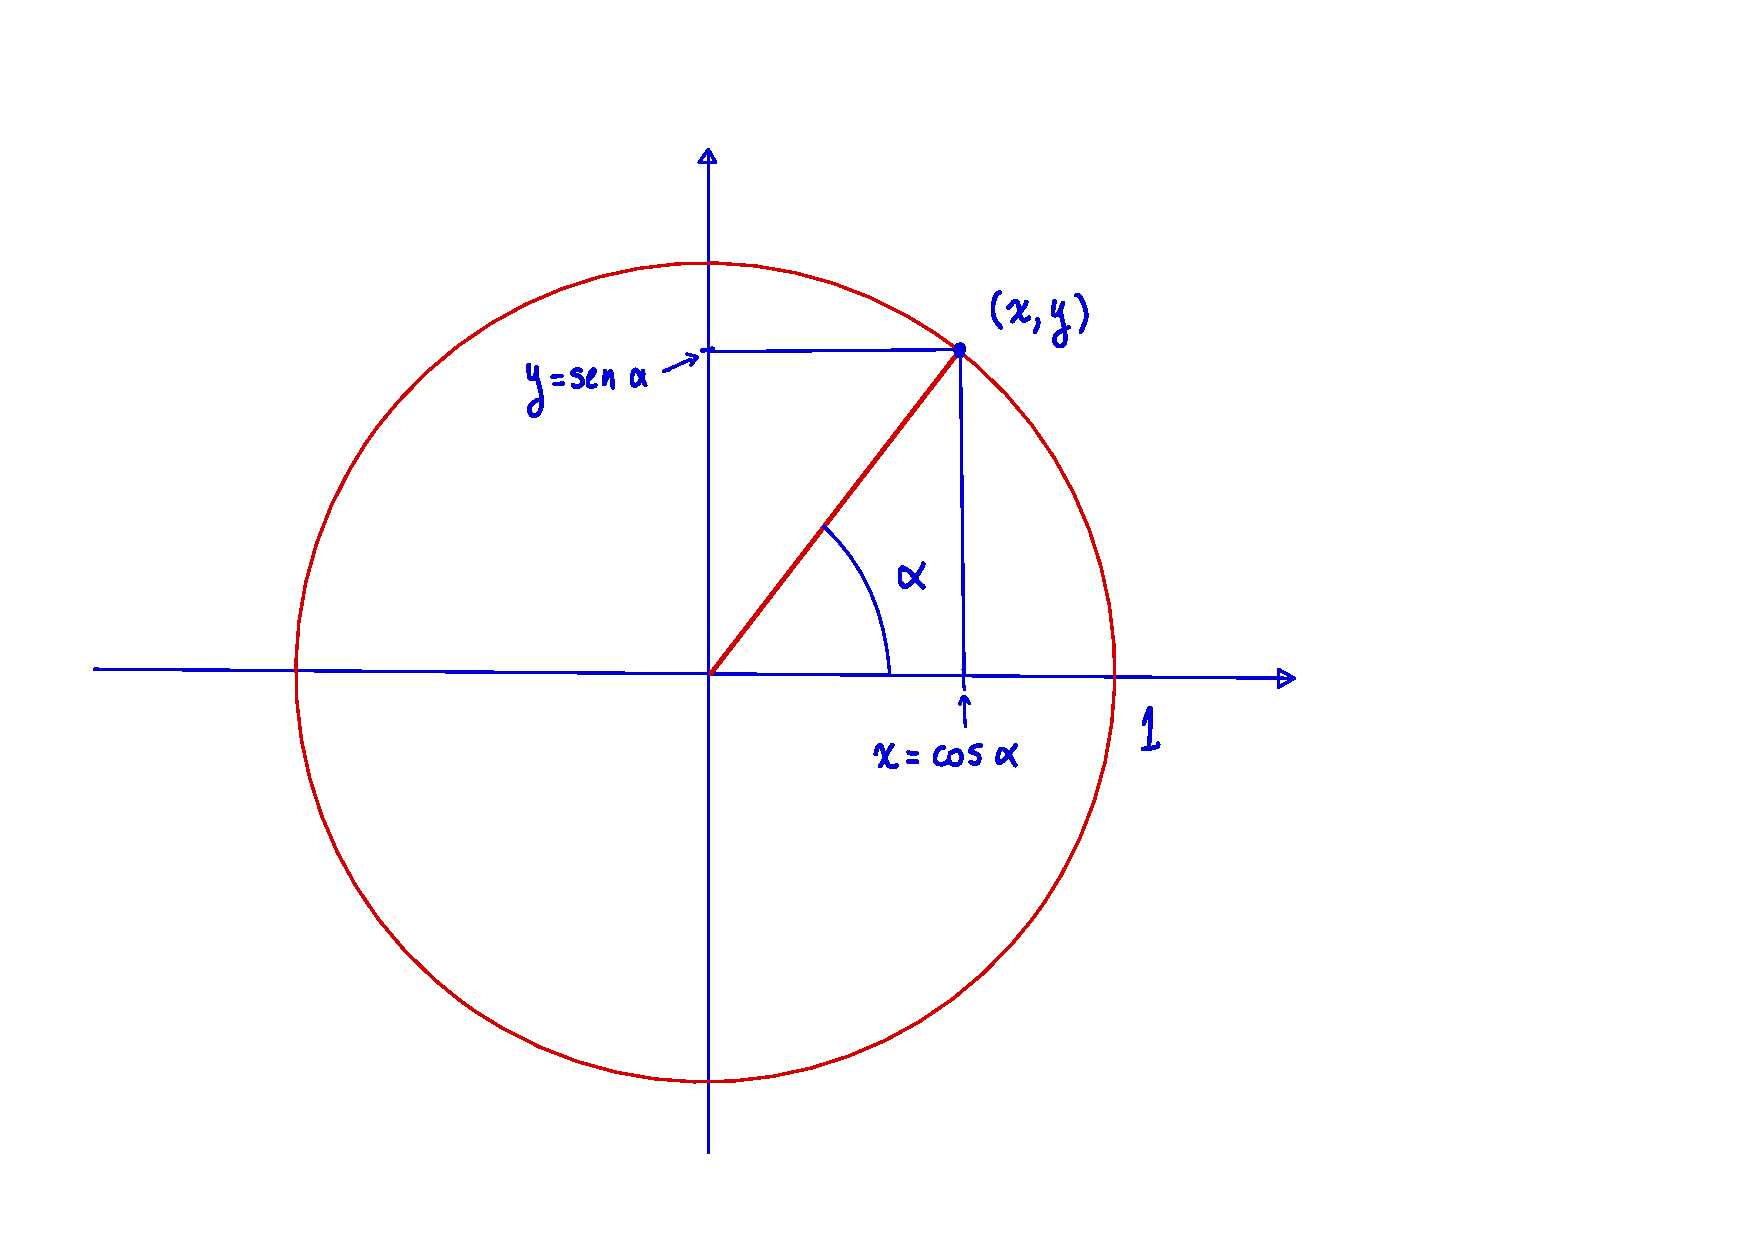
\includegraphics[width=.8\textwidth]{pics/trigonometricas.pdf}}

Dado un ángulo $\alpha\in\R$, giramos el segmento que une el origen de coordenadas con el punto $(1,0)$ un ángulo $\alpha$ alrededor del origen, en sentido positivo (antihorario) si $\alpha>0$ y negativo (horario) si $\alpha<0$. El punto $(1,0)$ va a parar a un punto $(x,y)$ de la circunferencia unitaria, es decir $x^2+y^2=1$. Definimos entonces las funciones 
\[
\cos\alpha=x,\qquad \sen\alpha=y,
\]
con dominio todo el conjunto de los reales.
Y a partir de estas, definimos las demás funciones trigonométricas:
\begin{align*}
    \tan \alpha &= \frac{\sen\alpha}{\cos\alpha}
    & \cotan\alpha &= \frac{\cos\alpha}{\sen\alpha}
    \\
    \sec\alpha&= \frac{1}{\cos\alpha}
    & \cosec\alpha &= \frac{1}{\sen\alpha}.
\end{align*}
El dominio de estas funciones es todo $\R$ excepto los puntos donde los denominadores de anulan.

Comenzamos ahora a estudiar la continuidad de la función $f(x)=\sen(x)$. Consideremos $x\in(-\pi/2,\pi/2)$. 
Cuando medimos el ángulo en radianes, la medida del ángulo en radianes $x$ coincide con la longitud del arco de circunferencia subtendido. Por lo tanto, para $0\le x<\pi/2$ resulta que $0\le \sen(x)\le x$.

\centerline{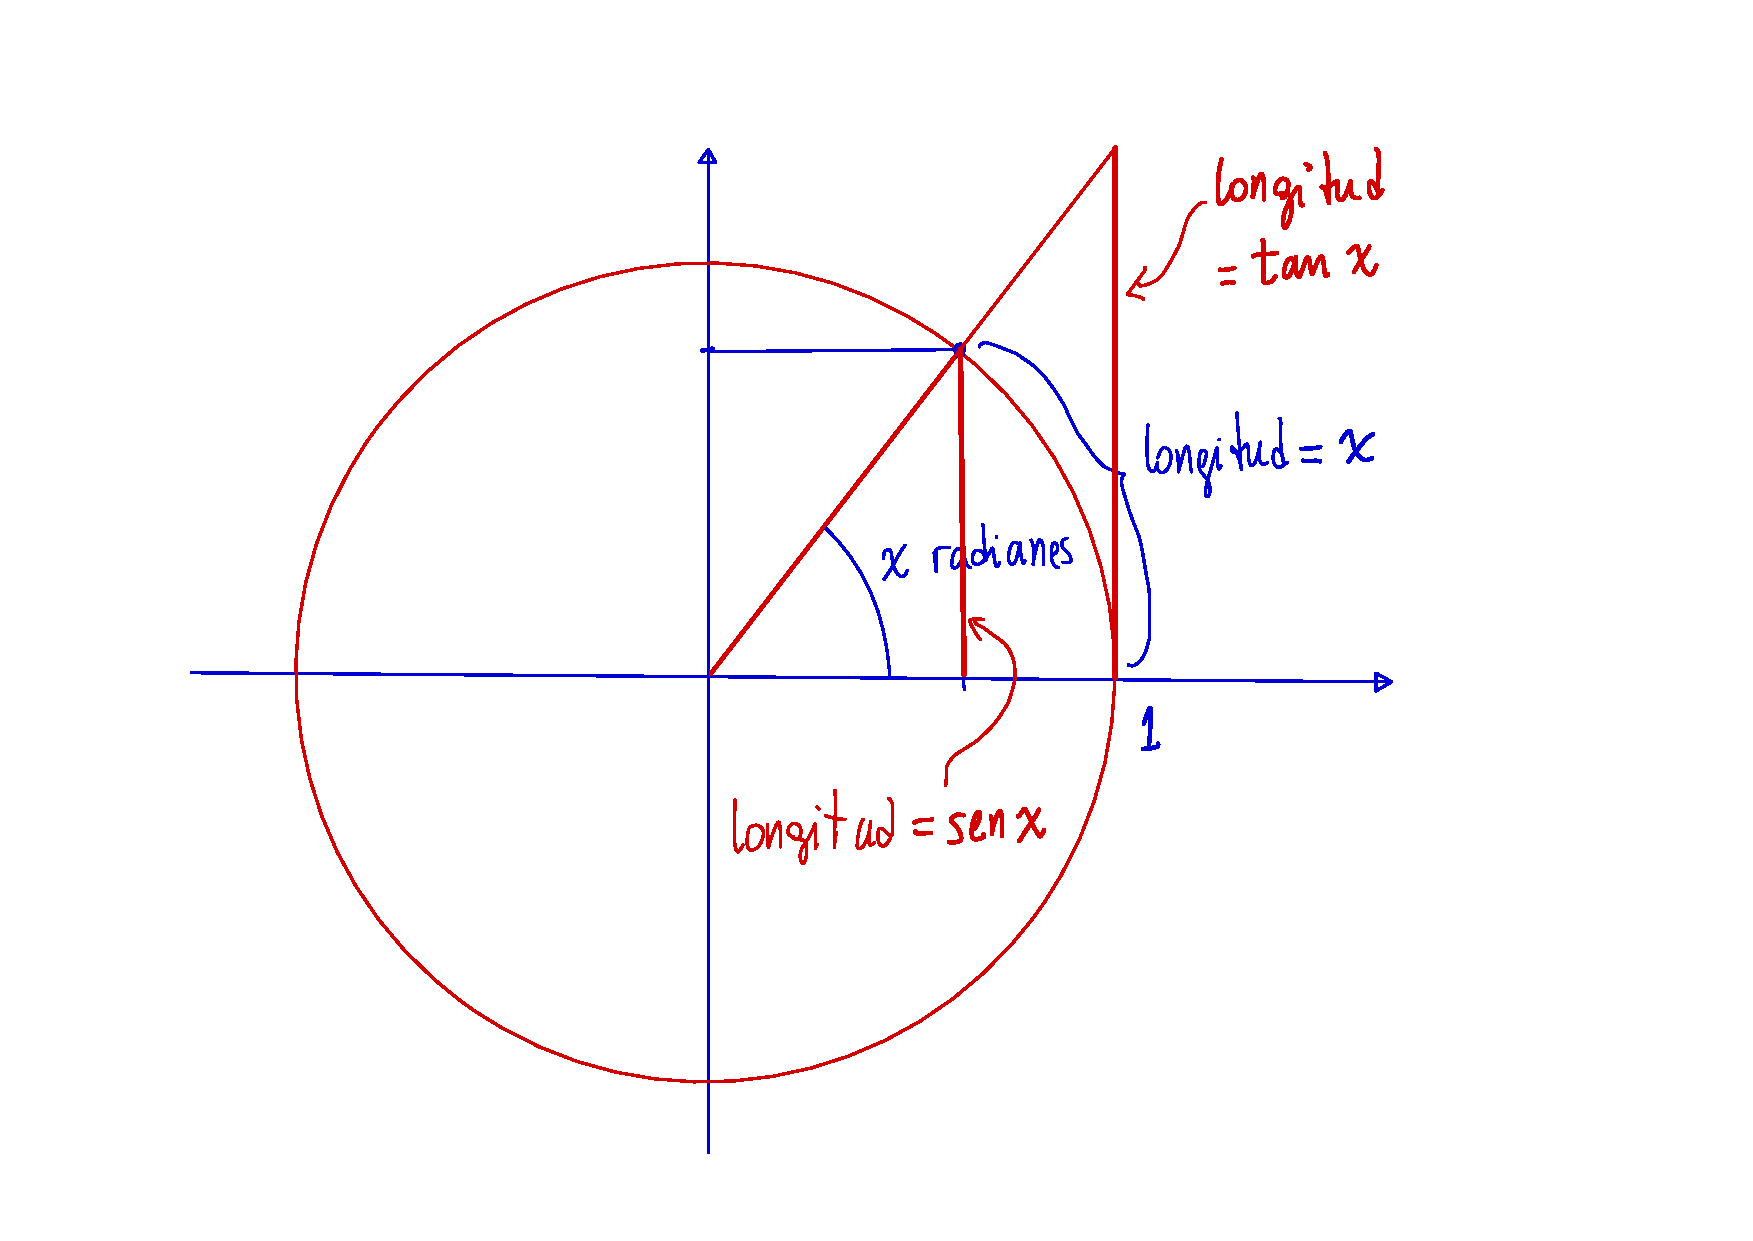
\includegraphics[width=.8\textwidth]{pics/seno-continuo.pdf}}

Utilizando ahora que la función seno es \emph{impar}, tenemos que para $-\pi/2<x<0$ resulta $\sen(x)=-\sen(-x)$ y por lo recién visto $0\le \sen(-x)\le -x$.
Por lo tanto,
\[
|\sen(x)|\le |x|, \qquad\text{para todo $x\in(-\pi/2,\pi,2)$}. 
\]
Esto implica que 
\[
-|x|\le \sen(x) \le |x|, \qquad\text{para todo $x\in(-\pi/2,\pi,2)$},
\]
y por la propiedad del emparedado, $\lim_{x\to0}\sen(x)=0=\sen(0)$, por lo que la función seno resulta continua en $x_0=0$.

Ahora bien, por identidades trigonométricas
\[
\sen(x)-\sen(x_0) = 2 \cos\frac{x+x_0}2 \sen\frac{x-x_0}2,
\]
y por lo tanto, como $|\cos(y)|\le 1$ cualquiera sea $y\in\R$,
\begin{align*}
|\sen(x)-\sen(x_0)| 
&= 2 \Big|\cos\frac{x+x_0}2\Big| \, \Big|\sen\frac{x-x_0}2\Big|
\\
&\le 2 \Big|\sen\frac{x-x_0}2\Big| 
\le 2 \Big|\frac{x-x_0}2\Big| ,
\end{align*}
si $|x-x_0|<\pi/2$. Esto muestra que $\D\limxo \big(\sen(x)-\sen(x_0)\big)=0$ o lo que es lo mismo 
\[
\limxo \sen(x)=\sen(x_0), \qquad \text{cualquiera sea $x_0\in\R$}.
\]
Por lo tanto, la función $f(x)=\sen(x)$ es continua en $\R$.
De manera similar, utilizando que
\[
\cos(x)-\cos(x_0) = -2 \sen\frac{x+x_0}2 \sen\frac{x-x_0}2,
\]
se puede probar que 
\[
\limxo \cos(x)=\cos(x_0), \qquad \text{cualquiera sea $x_0\in\R$},
\]
y por lo tanto, la función $f(x)=\cos(x)$ es continua en $\R$.

El resto de las funciones trigonométricas, como son cocientes de estas, resultan continuas en todo su dominio de definición, es decir, en todo $\R$, excepto en aquellos puntos donde el denominador se anula.

Como último ejemplo, estudiemos la continuidad de la función $f:\R\setminus\{0\}\to\R$ definida por
\[
f(x)=\frac{\sen(x)}{x}.
\]
Claramente esta función es continua en $\R\setminus\{0\}$ porque es el cociente de funciones continuas; notar que hemos quitado $x_0=0$ ya que allí el denominador de anula.

A priori no sabemos si existe $\D\lim_{x\to0}\frac{\sen(x)}{x}$ ya que tanto el numerador como el denominador tienden a cero.
Afirmamos que
\[
\lim_{x\to0}\frac{\sen(x)}{x}=1.
\]
Para ver que es así, notemos que para $0<x<\pi/2$, se cumple que 
\[
\sen(x)<x<\tan (x).
\]
Luego, dividiendo por $\sen(x)$ tenemos que
\[
1<\frac{\sen(x)}{x} < \frac{\tan(x)}{\sen(x)} = \frac{1}{\cos(x)}.
\]
Observamos ahora que como el coseno es continuo $\lim_{x\to 0^+}\cos(x)=\cos(0)=1$ y por el teorema del emparedado
\[
\lim_{x\to0^+}\frac{\sen(x)}{x}=1.
\]
Si $x<0$ resulta que $\D \frac{\sen(x)}{x} = \frac{\sen(-x)}{-x}$ y entonces
\[
\lim_{x\to0^-}\frac{\sen(x)}{x}
=\lim_{x\to0^-}\frac{\sen(-x)}{-x}
=\lim_{y\to0^+}\frac{\sen(y)}{y}=1.
\]
En definitiva, $\D f(x)=\frac{\sen(x)}{x}$ tiene una discontinuidad \emph{evitable} en $x_0=0$, que se evita definiendo $f(0)=1$.


\subsubsection*{Ejercicios de la sección~\getcurrentref{chapter}.\getcurrentref{section}}

\begin{enumerate}
\item Estudiar la continuidad en cada $x_0\in\R$ de las siguientes funciones:
\begin{multicols}{2}
\begin{enumerate}
    \item $\D f(x)=\frac{1}{x^2}$
    \item $\D f(x)=\begin{cases}
        \frac{x^2-3x+2}{x^2-4x+4}, \quad&\text{si }x > 3,\\
        2-x^2, \quad&\text{si }x \le 3
    \end{cases}$
    \item $\D f(x)=\begin{cases}
        \frac{x+3}{x-1}, \quad&\text{si }x\neq 1,\\
        2, \quad&\text{si }x = 1
    \end{cases}$
    \item $\D f(x)=\begin{cases}
        x^2+4, \quad&\text{si }x > 0,\\
        2x-1, \quad&\text{si }x <0
    \end{cases}$
    \item $\D f(x)=\frac{(x-3)^2}{x^2-9}$
    \item $\D f(x)=\frac{x^2}{\sqrt{1+x^2}-1}$
    \item $\D f(x)=\frac{\sqrt{1+x}-\sqrt{1-x}}{x}$
    \item $\D f(x)=\frac{4-\sqrt{6+x}}{2-\sqrt{x-2}}$
\end{enumerate}
\end{multicols}

\item Calcular los siguientes límites:
\begin{multicols}{2}
\begin{enumerate}
    \item $\D \lim_{x\to 2^+} \sqrt{\frac{x^3-9}{x^2-4}}$
    \item $\D \lim_{x\to 3} \sqrt{\frac{x^3-27}{x^2-9}}$
    \item $\D \lim_{x\to 0^+} \frac{\sqrt{1+x^2}-1}{x}$
    \item $\D \lim_{x\to 1} \frac{\sqrt{x+2}-\sqrt{3x+1}}{\sqrt{x-1}}$
    \item $\D \lim_{x\to 2^-} \sqrt{2-x}-\lfloor x+1 \rfloor$
    \item $\D \lim_{x\to 0} \frac{\sen 3x}{\sen 5x}$
    \item $\D \lim_{x\to 0} \frac{1-\cos x}x$
    \item $\D \lim_{x\to 0^+} \left(\sen x\right)^{\frac{\sen x}{x}}$
    \item $\D \lim_{x\to 0} \frac{\sen 3x}{x^2+\sqrt{x}}$
    \item $\D \lim_{x\to \pi/2} \frac{\cos x}{x-\pi/2}$
    \item $\D \lim_{x\to 0} \frac{\tan 2x}{3x}$
    \item $\D \lim_{x\to 0} \frac{x\, \sen x}{1-\cos x}$
    \item $\D \lim_{x\to 0} \frac{\ln(1+x)}{x}$
    \item $\D \lim_{x\to +\infty} \big(\ln(x+1)-\ln(x+2)\big)$
    \item $\D \lim_{x\to +\infty} \frac{\ln\big(1+e^x\big)}{x}$
    \item $\D \lim_{x\to -\infty} \frac{\ln\big(1+e^x\big)}{x}$
    \item $\D \lim_{x\to 0} \frac1x \, \ln\sqrt{\frac{1+x}{1-x}}$
    \item $\D \lim_{x\to 0} \left(1+x\right)^{\frac1{\sen x}}$
    \item $\D \lim_{x\to 0} \left(\cos x\right)^{1/x}$
    \item $\D \lim_{x\to +\infty} x^2 \big(\ln(x^2+4)-\ln x^2\big) $
\end{enumerate}
\end{multicols}


\end{enumerate}


    
\section{Funciones continuas en un intervalo cerrado}

Consideraremos en esta sección funciones $f$ que sean continuas en todos los puntos de un intervalo \emph{cerrado} $[a,b]$.
Hasta ahora solo hemos hablado de continuidad en intervalos abiertos; para definir continuidad en un punto $x_0$ hemos pedido que $x_0\in(a,b)$ con $(a,b)$ un intervalo abierto donde la función está definida.

\begin{definition}[Continuidad en un intervalo cerrado]
Decimos que una función $f:[a,b]\to\R$ es continua en $[a,b]$ si:
\begin{itemize}
    \item Es continua en $x_0$, para todo $x_0\in(a,b)$.
    \item Es continua \emph{por derecha} en $a$: $\D\lim_{x\to a^+}f(x)=f(a)$.
    \item Es continua \emph{por izquierda} en $b$: $\D\lim_{x\to b^-}f(x)=f(b)$.
\end{itemize}
\end{definition}

Las funciones continuas en intervalos cerrados tienen tres propiedades muy importantes. Para establecer la primera, necesitamos recordar que una función $f:A\to\R$ se dice \emph{acotada} si existen números reales $m$ y $M$ tales que 
\[
m\le f(x) \le M, \qquad\text{para todo $x\in A$}.
\]
En otras palabras, $f:A\to\R$ es acotada si la imagen de $f$, $\im(f)=\{f(x):x\in A\}$ es un conjunto acotado de $\R$.
Veamos el primer teorema importante.

\begin{theorem}\label{T:continua->acotada}
    Si $f:[a,b]\to\R$ es continua en $[a,b]$, entonces es acotada en $[a,b]$.
\end{theorem}

\begin{proof}
    La demostración de este teorema será vista en las clases de coloquios. El lector interesado puede encontrarla en el libro~\cite{Noriega}, como Teorema 6.25.
\end{proof}

Sigamos pensando en una función $f:[a,b]\to\R$ continua en el intervalo cerrado $[a,b]$. Ya vimos que es necesariamente acotada. Por lo tanto el conjunto $\im(f)$ es acotado, y entonces tiene supremo e ínfimo.
Lo que afirma el segundo resultado importante de esta sección es que ese supremo y ese ínfimo son, respectivamente, un máximo y un mínimo, es decir, existe $x_m\in[a,b]$ tal que $f(x_m)\le f(x)$, para todo $x\in[a,b]$, y existe $x_M\in[a,b]$ tal que $f(x_M)\ge f(x)$, para todo $x\in[a,b]$. Esto suele decirse de la siguiente forma: \emph{$f$ alcanza un máximo y un mínimo en $[a,b]$}.

\begin{theorem}\label{T:continua->maximo y minimo}
    Si $f$ es una función continua en un intervalo cerrado $[a,b]$, entonces alcanza un máximo y un mínimo en $[a,b]$.
\end{theorem}

\begin{proof}
    Al ser $f$ continua en $[a,b]$, el conjunto
    \[
    \im(f)=\{f(x) : x\in[a,b]\}
    \]
    es acotado inferior y superiormente, y claramente no vacío.
    Por lo tanto, existen
    \[
    m=\inf \im(f)
    \qquad\text{y}\qquad
    M=\sup \im(f).
    \]
    Probemos ahora que existe $x_M\in[a,b]$ tal que $f(x_1)=M$.
    Si no fuese cierto, entonces $f(x)<M$, para todo $x\in[a,b]$ y entonces $M-f(x)\neq 0$, para todo $x\in[a,b]$.
    Consideramos entonces la función
    \[
    g(x)=\frac{1}{M-f(x)},
    \]
    que resulta continua en $[a,b]$ porque es cociente de funciones continuas y el denominador no se anula en ese intervalo.
    Pero entonces, por el Teorema~\ref{T:continua->acotada} la función $g$ es acotada en $[a,b]$. En particular, existe $K>0$ tal que 
    \[
    g(x)=\frac{1}{M-f(x)}\le K,
    \qquad\text{para todo $x\in[a,b]$}.
    \]
    Esto a su vez implica que $\frac1K \le M -f(x)$ por lo que
    \[
    f(x)\le M-\frac1K,
    \qquad\text{para todo $x\in[a,b]$}.
    \]
    Es decir, $M-\frac1K$ es una cota superior de $\im(f)$.
    Como $M-\frac1K<M$ esto contradice que $M=\sup\im(f)$.
    Esta contradicción proviene de suponer que no existe $x_M\in[a,b]$ tal que $f(x_M)=M$.
    
    Luego, existe $x_M\in[a,b]$ tal que $f(x_M)=M$.
    Como $M$ es el supremo de la función $f$, resulta que es cota superior de $\im(f)$ y por lo tanto
    \[
    f(x_M)\ge f(x), 
    \qquad\text{para todo $x\in[a,b]$}.
    \]

    Razonando análogamente con la función
    \[
    h(x) = \frac1{f(x)-m}
    \]
    se prueba que existe $x_m\in [a,b]$ tal que $f(x_m)=m$, y por lo tanto
    \[
    f(x_m)\le f(x), 
    \qquad\text{para todo $x\in[a,b]$}.
    \qedhere
    \]
\end{proof}

Antes de ver el próximo teorema, conviene hacer algunas observaciones.

La idea original, intuitiva, geométrica, de una función continua, es la de una función cuya representación gráfica se puede hacer sin levantar el lápiz, es decir, que en la representación gráfica no haya saltos (como los que tiene la función $f(x)=\lfloor x\rfloor$) ni puntos donde la función se vaya al infinito (como $f(x)=\frac1x$ en $x=0$).

El siguiente teorema confirma nuestra intuición acerca de este significado geométrico de la continuidad.

\begin{theorem}[Teorema de Bolzano]\label{T:Bolzano}
Sea $f$ una función continua en $[a,b]$ tal que $f(a)<0$ y $f(b)>0$. Entonces existe $c\in(a,b)$ tal que $f(c)=0$.
\end{theorem}

Este teorema afirma que si un punto de la gráfica de una función continua está por debajo del eje de abscisas y otro está por encima, entonces dicha gráfica debe cortar el eje de abscisas en algún punto.

\begin{proof}
    Consideremos el conjunto
    \[
    A=\{x\in[a,b]:f(x)<0\}.
    \]
    Este conjunto está acotado superiormente por $b$ y es no vacío ya que $a\in A$.
    Entonces existe $c=\sup A$. Afirmamos que ese $c$ cumple $f(c)=0$. Para probarlo, descartaremos las posibilidades $f(c)<0$ y $f(c)>0$.

    Si fuera $f(c)<0$, entonces, por la Proposición~\ref{P:continua:cota en intervalo}, existe $\delta>0$ tal que $f(x)<0$ para todo $x\in(c-\delta,c+\delta)$. Tomamos $x_1=c+\delta/2$ que cumple $c<x_1<c+\delta$ y entonces $f(x_1)<0$. Luego $x_1>c$ y $x_1\in A$, lo que contradice que $c=\sup A$ (contradice que $c$ sea cota superior de $A$). Por lo tanto, no es posible que $f(c)<0$.

    Supongamos ahora que $f(c)>0$, nuevamente por la Proposición~\ref{P:continua:cota en intervalo}, existe $\delta>0$ tal que $f(x)>0$ para todo $x\in (c-\delta,c+\delta)$. Tomamos $x_2=c-\delta/2$ que cumple $c-\delta<x_2<c$ y entonces $x_2<c$ y no podría ser cota superior de $A$ (ya que al ser $c=\sup A$ es la menor de las cotas superiores).
    Como $x_2<c$ no es cota superior, debe existir $x_3\in A$ tal que $x_2<x_3\le c$. Pero $x_3\in(c-\delta,c+\delta)$ por lo que $f(x_3)>0$, lo que contradice que $x_3\in A$.
    Por lo tanto, no es posible que $f(c)>0$.
\end{proof}

A partir de este teorema, concluimos el famoso \emph{Teorema del Valor Intermedio (TVI)}.

\begin{corollary}[Teorema del Valor Intermedio]\label{TVI}
Sea $f$ una función continua en $[a,b]$ tal que $f(a)<f(b)$.
Si $d$ es cualquier número tal que $f(a)<d<f(b)$, entonces existe $c\in(a,b)$ tal que $f(c)=d$.
\end{corollary}

\begin{proof}
    Definimos la función auxiliar
    \[
    g(x) = f(x)-d.
    \]
    Esta función es también continua en $[a,b]$ y cumple 
    \[
    g(a) = f(a)-d < 0,
    \qquad\text{y}\qquad
    g(b) = f(b)-d > 0.
    \]
    Luego, por el Teorema~\ref{T:Bolzano}, existe $c\in(a,b)$ tal que $g(c)=0$.
    Como $g(c)=f(c)-d$, $g(c)=0$ equivale a $f(c)=d$.
\end{proof}

Como consecuencia de este último resultado, se obtiene la continuidad de algunas funciones.

\begin{theorem}[Continuidad de la función inversa]
Si $f$ es una función continua en $[a,b]$ y estrictamente creciente (o estrictamente decreciente) en $[a,b]$, entonces
\begin{enumerate}[{\bf (a)}]
    \item $f:[a,b]\to[f(a),f(b)]$ ($f:[a,b]\to[f(b),f(a)]$) es biyectiva.
    \item $f^{-1}:[f(a),f(b)]\to [a,b]$ ($f^{-1}:[f(b),f(a)]\to [a,b]$) es continua.
\end{enumerate}
\end{theorem}

\begin{proof}
    Demostremos el caso en que $f$ es estrictamente creciente (el caso de $f$ estrictamente decreciente es análogo).

\begin{enumerate}[{\bf (a)}]
\item $f$ es inyectiva, dado que es \emph{estrictamente} creciente. $f$ es sobreyectiva, pues si $y\in (f(a),f(b))$ resulta $f(a)<y<f(b)$ y por lo tanto, por el Teorema~\ref{TVI} existe $x\in(a,b)$ tal que $f(x)=y$.

\item Ya que $f$ es biyectiva, tiene función inversa $f^{-1}:[f(a),f(b)]\to [a,b]$. Veamos que $f^{-1}$ es continua en cada $y_0\in(f(a),f(b))$. 

Sea $y_0\in(f(a),f(b))$ y sea $\epsilon>0$; suponemos que $\epsilon<\min\{b-x_0,x_0-a\}$ ya que lo importante es lo que ocurre para $\epsilon$ pequeño. Al ser $f$ sobreyectiva, existe $x_0\in(a,b)$ tal que $f(x_0)=y_0$.
Sean
\[
d_1=f(x_0-\epsilon), 
\qquad
d_2=f(x_0+\epsilon),
\]
y sea
\[
\delta=\min\{d_2-y_0,y_0-d_1\}
\qquad\text{luego $\delta\le d_2-y_0$ y $\delta\le y_0-d_1$}.
\]
Queremos probar que $|y-d|<\delta$ implica $\big|f^{-1}(y)-f^{-1}(y_0)\big|<\epsilon$.
Para ello, sea $y$ tal que $|y-d|<\delta$, o sea $y_0-\delta<y<y_0+\delta$.
Como $f$ es sobreyectiva, existe $c\in(a,b)$ tal que $f(c)=y$.
Siendo $y_0-\delta<y<y_0+\delta$, resulta $d_1<y<d_2$, o sea
\[
d_1=f(x_0-\epsilon)<y=f(c)<f(x_0+\epsilon)=d_2.
\]
Como $f$ es estrictamente creciente, debe ser
\[
x_0-\epsilon < c < x_0+\epsilon 
\quad\implies\quad
|c-x_0|<\epsilon.
\]
Pero $c=f^{-1}(y)$ y $x_0=f^{-1}(y_0)$ por lo que
\[
\big|f^{-1}(y)-f^{-1}(y_0)\big|<\epsilon.
\]
Hemos demostrado que dado $\epsilon>0$ existe $\delta$ tal que
\[
\big|f^{-1}(y)-f^{-1}(y_0)\big|<\epsilon,
\qquad\text{para todo $y$ tal que $|y-y_0|<\delta$}.
\]
Es decir, $f\inv$ es continua en $y_0$, cualquiera sea $y_0\in(f(a),f(b))$.
La demostración de que $f\inv$ es continua por derecha en $y_a=f(a)$ y que es continua por izquierda en $y_b=f(b)$ es análoga.
\end{enumerate}
\end{proof}


\subsubsection*{Ejercicios de la sección~\getcurrentref{chapter}.\getcurrentref{section}}

\begin{enumerate}
\item Para las siguientes funciones, determinar cuáles son acotadas superiormente e inferiormente en el intervalo indicado y si alcanzan su máximo y mínimo en algún punto del intervalo:

\begin{multicols}{2}
\begin{enumerate}
    \item $f(x)= x^2$ en $(-1,1)$
    \item $f(x)= x^2$ en $[-1,1]$
    \item $f(x)= x^3$ en $(-1,1)$
    \item $f(x)= x^3$ en $[-1,1]$
    \item $\D f(x)= \frac1x$ en $(0,1)$
    \item $\D f(x)= \frac1x$ en $(0,1]$
    \item $f(x)= \sqrt{x}$ en $(0,1)$
    \item $f(x)= \sqrt{x}$ en $[0,1]$
\end{enumerate}   
\end{multicols}



\item Probar que la ecuación $x^3-3x+1=0$ tiene una raíz real en el intervalo $(1,2)$.

\item Probar que existe $x\in\R$ tal que $\cos x=x$.

\item Probar que si $p(x)$ es un polinomio \emph{mónico} de grado impar, entonces existe $x_0\in\R$ tal que $p(x_0)=0$.

\item Probar que si $p(x)$ es un polinomio de grado impar, entonces existe $x_0\in\R$ tal que $p(x_0)=0$.

\item Probar que si $n$ es un número natural, entonces en el intervalo $\D\Big(n\pi-\frac\pi2,n\pi+\frac\pi2\Big)$ hay un $x$ que cumple $\tan x=-x$. Ayudarse con GeoGebra, graficar las funciones $\tan x$ y $-x$ para ver cómo usar el Teorema~\ref{TVI} para demostrar lo pedido.

\item Demostrar que existe un número real $x$ tal que
\[
x^{179} + \frac{163}{1+x^2+\sen^2 x} = 119.
\]

\item Supongamos que $f$ y $g$ son continuas en $\R$ y que $f(a)>g(a)$ para algún $a\in\R$ y $f(b)<g(b)$ para algún $b\in\R$. Probar que existe $x\in\R$ tal que $f(x)=g(x)$.

\item Supongamos que $f:\R\to\R$ es continua y que $f(x)\in\Q$, para todo $x\in\R$. Probar que entonces $f$ es constante.

\end{enumerate}

\section{El método de Bisección}

Como consecuencia del Teorema del Valor Intermedio se obtiene un método para calcular de manera aproximada soluciones de ecuaciones para las cuales no hay un fórmula precisa.
Por ejemplo, las ecuaciones
\[
\cos x = x,\qquad
\ln x = \frac 1x,\qquad
x = e^x-2, \qquad
x\sen(x)=1.
\]

Todas estas ecuaciones pueden escribirse como
\begin{equation}\label{eq:ecuacion1}
f(x) = 0.
\end{equation}
En efecto, si restamos el lado derecho del izquierdo en cada ecuación de los ejemplos presentados, tenemos
\[
\cos x - x=0,\qquad
\ln x - \frac 1x=0,\qquad
x - e^x + 2=0, \qquad
x\sen(x)-1=0.
\]

Un corolario inmediato del Teorema del Valor Intermedio~\ref{TVI} es el siguiente:

\begin{corollary}
Si $f:[a,b] \to \R$ es una función continua y $f(a)$ y $f(b)$ tienen signo opuesto ($f(a)\cdot f(b) < 0$), entonces existe $c \in (a,b)$ tal que $f(c) = 0$.
\end{corollary}

La idea del método de bisección es comenzar con un intervalo $[a,b]$ tal que $f(a)$ y $f(b)$ tienen signo opuesto, es decir, tenemos localizada una raíz en el intervalo $[a,b]$. Luego, ir reduciendo sistemáticamente la longitud del intervalo donde estamos seguros que hay una raíz, hasta que tengamos una tolerancia aceptable, es decir, un intervalo tan pequeño donde se encuentra la raíz que es satisfactorio para el problema en cuestión.
La manera de subdividir el intervalo consiste en tomar el punto medio del intervalo 
\[
m = \frac{a+b}2,
\]
y luego analizar las tres posibilidades que pueden darse
\begin{enumerate}[(1)]
\item Si $f(a)$ y $f(m)$ tienen signos opuestos, entonces hay un cero en $[a,m]$.
\item Si $f(m)$ y $f(b)$ tienen signos opuestos, entonces hay un cero en $[m,b]$.
\item Si $f(m) = 0$, entonces $m$ es la solución buscada.
\end{enumerate}

Si ocurre el caso (3), hemos encontrado la raíz (debemos aclarar que esto no se da casi nunca, pero puede ocurrir).
Si ocurre el caso (1) o el caso (2), entonces hemos encontrado un intervalo cuyo ancho es la mitad que el original y contiene una raíz. Para continuar el proceso, renombramos el nuevo intervalo más pequeño como $[a,b]$ y repetimos el procedimiento hasta que el intervalo sea tan pequeño como deseamos. Puesto que el proceso de bisección genera una sucesión de intervalos encajados, con sus correspondientes puntos medios, usaremos la siguiente notación para tener un registro de los detalles del proceso:\\

\frame{
\begin{minipage}{.9\textwidth}
${}$	

\centerline{\bf Método de Bisección}
\begin{itemize}
\item $[a_0,b_0]$ es el intervalo de partida y $m_0 = \D\frac{a_0+b_0}2$ es su punto medio.
\item $[a_1,b_1]$ es el segundo intervalo (coincide con $[a_0,m_0]$ o con $[m_0,b_0]$) y $m_1$ es su punto medio. El intervalo $[a_1,b_1]$ es la mitad de ancho que $[a_0,b_0]$.
\item $\cdots$
\item Después de llegar al intervalo $[a_n,b_n]$, en el que también se localiza un cero, y cuyo punto medio es $m_n$, se construye el intervalo $[a_{n+1},b_{n+1}]$, en el que también hay un cero y mide la mitad de $[a_n,b_n]$.\\
\end{itemize}
\end{minipage}
}

A partir de este procedimiento resulta que
\[
a_0 \le a_1 \le \dots \le a_n \le \dots \le b_n \le \dots\le b_1 \le b_0.
\]
Y además, hay una raíz $c$ que satisface $a_n \le c \le b_n$.

Es importante que nos detengamos un momento a pensar cómo se define el intervalo $[a_{n+1},b_{n+1}]$ a partir del $[a_n,b_n]$:
\begin{itemize}
\item Definimos $m_n = \D\frac{a_n+b_n}2$.
\item Si $f(a_n)\cdot f(m_n) < 0$ (entonces hay una raíz en el intervalo $[a_n,m_n] $)
\begin{itemize}
\item Definimos $[a_{n+1},b_{n+1}] = [a_n,m_n]$ (o $a_{n+1} = a_n$ y $b_{n+1} = m_n$)
\end{itemize}
\item Si no, (entonces ocurre que $f(m_n)\cdot f(b_n) < 0$)
\begin{itemize}
\item Definimos $[a_{n+1},b_{n+1}] = [m_n,b_n]$ (o $a_{n+1} = m_n$ y $b_{n+1} = b_n$)
\end{itemize}
\item Si no ocurre ninguna de las anteriores, resulta $f(m_n)=0$. 
\begin{itemize}
\item Entonces $m_n$ es la solución. FIN.
\end{itemize}
\end{itemize}

Observamos que con este procedimiento, en cada paso, la longitud del intervalo se reduce a la mitad, es decir
\[
|b_{n+1} - a_{n+1}| = \frac{|b_n-a_n|}2.
\]

Por lo tanto, después de $n$ pasos, la longitud del intervalo es
\[
|b_n - a_n| = \frac{|b_0-a_0|}{2^n} = \left(\frac12\right)^n |b_0-a_0|.
\]

Como $m_n$ está en el centro del intervalo $[a_n,b_n]$ resulta que la distancia a la raíz $p$ es menor o igual a la mitad de la longitud del intervalo $[a_n,b_n]$, es decir
\[
|p - m_n| \le \frac{|b_n-a_n|}2 = \left(\frac12\right)^{n+1} |b_0-a_0|.
\]

Resumimos todo lo analizado hasta ahora en el siguiente teorema.

\begin{theorem}[Convergencia del método de bisección]
Supongamos que $f:[a,b] \to \R$ es continua y que $f(a)$ y $f(b)$ tienen signos distintos.
Sea $\{ m_n \}_{n\ge 0}$ la sucesión de puntos medios de los intervalos generados por el método de bisección. Entonces existe una raíz $c$ de la ecuación $f(x)=  0$ (es decir, $f(c)=0$) en $[a,b]$ tal que $m_n \to c$, cuando $n\to\infty$ y además
\[
|c - m_n | \le \left(\frac12\right)^{n+1} |b-a|, \qquad n=0,1,2,\dots.
\]
\end{theorem}

\subsubsection*{Ejercicios de la sección~\getcurrentref{chapter}.\getcurrentref{section}}

\begin{enumerate}
\item Programar en \verb|Python| el método de bisección.

\item Utilizar el método programado en el punto anterior para hallar una solución aproximada de cada una de las siguientes ecuaciones en el intervalo indicado. Se pide una solución con un error menor a $10^{-6}$.
\begin{multicols}{2}
    \begin{enumerate}
        \item $\D \cos x = x$ en $[0,\pi/2]$
        \item $\D \ln x = 1/x$ en $[1,3]$
        \item $\D x=e^x-2$ en $[0,2]$
        \item $\D x\sen(x)=1$ en $[0,2]$
    \end{enumerate}
\end{multicols}

\end{enumerate}

\begin{comment}

\section{Continuidad uniforme (LMA???)}


\subsubsection*{Ejercicios de la sección~\getcurrentref{chapter}.\getcurrentref{section}}

\begin{enumerate}
\item 
\end{enumerate}




\end{comment}


%%%%%%%%%%%%%%%%%%%%%% ejercicios del capítulo
\subsection*{Ejercicios del capítulo~\getcurrentref{chapter}}


\begin{enumerate}
\item Demostrar que la función $f(x)=-3x+10$ es continua en $x_0$, para todo $x_0\in\R$.

\item 
Consideremos la función $f:(0,\infty)\to(0,\infty)$ dada por
$f(x)=\frac1x$.
\begin{enumerate}
    \item Demostrar que es continua en $x_0=2$;
    \item Demostrar que es continua en $x_0=1$;
    \item Demostrar que es continua en $x_0=1/2$;
    \item ¿Se anima a demostrar que es continua en $x_0$, cualquiera sea  $x_0>0$?
\end{enumerate}

\item 
Consideremos la función $f:(0,\infty)\to(0,\infty)$ dada por
$f(x)=\sqrt x$.
\begin{enumerate}
    \item Demostrar que es continua en $x_0=2$;
    \item Demostrar que es continua en $x_0=1$;
    \item Demostrar que es continua en $x_0=1/2$;
    % \item Demostrar que es continua en $x_0=0$;
    \item ¿Se anima a demostrar que es continua en $x_0$, cualquiera sea $x_0\in(0,\infty)$?
\end{enumerate}

\item 
Consideremos la función 
\[
f(x) = \begin{cases}
    x\sen \frac1x,\quad &\text{si $x\neq 0$},
    \\
    0,\quad &\text{si $x = 0$},
    \end{cases}
\]
\begin{enumerate}
    \item Graficarla con GeoGebra
    \item Verificar con geogebra que 
    \[
    -|x| \le f(x) \le |x|,\quad \forall\xiR.
    \]
    \item Demostrar analíticamente que 
    \[
    -|x| \le f(x) \le |x|,\quad \forall\xiR.
    \]
    \item Verificar que $|f(x)-f(0)|\le |x-0|$, para todo \xiR.
    \item Demostrar que $f(x)$ es continua en $x_0=0$.
\end{enumerate}

\item 
Consideremos la función
\[
H(x) = \begin{cases}
    0, \quad &\text{si $x<0$},\\
    1, \quad &\text{si $x\ge0$},
\end{cases}
\]
\begin{enumerate}
    \item Demostrar que $H(x)$ es continua en $x_0$ para todo $x_0\neq 0$.
    \item Demostrar que $H(x)$ no es continua en $x_0=0$.
\end{enumerate}

\item \label{ej:sen1_x}
Consideremos la función 
\[
f(x) = \begin{cases}
    \sen \frac1x,\quad &\text{si $x\neq 0$},
    \\
    0,\quad &\text{si $x = 0$},
    \end{cases}
\]
\begin{enumerate}
    \item Graficarla con GeoGebra
    \item Demostrar que para cada $\delta>0$ existe $x_1\in(0,\delta)$ tal que $f(x_1)=1$.
    \item Demostrar que para cada $\delta>0$ existe $x_2\in(0,\delta)$ tal que $f(x_2)=-1$.
    \item Demostrar que $f(x)$ no es continua en $x_0=0$.
\end{enumerate}


\item Consideremos la función constante $f(x)=a$, para algún $a\in\R$. Demostrar usando la definición que $f$ es continua en $x_0$ para todo $x_0\in\R$.
\item Consideremos la función \emph{identidad} $f(x)=x$. Demostrar usando la definición que $f$ es continua en $x_0$ para todo $x_0\in\R$.
\item Demostrar que si $a$ y $b$ son números reales, entonces la función lineal $f(x)=ax+b$ es continua en $x_0$ para todo $x_0\in\R$.
Usar lo demostrado en los ejercicios anteriores y las propiedades vistas en esta sección.
\item Demostrar que si $a$, $b$ y $c$ son números reales, entonces la función cuadrática $f(x)=ax^2+bx+c$ es continua en $x_0$ para todo $x_0\in\R$.
Usar lo demostrado en los ejercicios anteriores y las propiedades vistas en esta sección.
\item\label{ej:polinomios-continuos} Demostrar que si $p(x)$ es una función polinomial, entonces $p$ es continua en $x_0$ para todo $x_0\in\R$ (Ayuda: usar inducción sobre el grado polinomial).
\item Demostrar que si $p(x)$ y $q(x)$ son funciones polinomiales, entonces la función racional $\frac pq$ es continua en $x_0$ para todo $x_0\in\R$, excepto para aquellos puntos donde $q(x)$ se anula. 


\item Demostrar usando la definición, que $\D\lim_{x\to 0^+} \sqrt{x} = 0$.

\item Demostrar usando el Teorema~\ref{T:TFLD} que no existe $\D\lim_{x\to 0^+}\cos\frac1x$.

\item Determinar (usando los límites que ya conocemos y las propiedades) los siguientes límites, considerando separadamente los casos $x_0\in\Z$ y $x_0\in\R\setminus\Z$:
\begin{multicols}{2}
    \begin{enumerate}
    \item $\D\lim_{x\to x_0^+} \big(x-\lfloor x \rfloor\big)$;
    \item $\D\lim_{x\to x_0^+} \big(|x|+\lfloor x \rfloor\big)$.
    \end{enumerate}
\end{multicols}

\item Determinar (usando los límites que ya conocemos y las propiedades) los siguientes límites, considerando separadamente los casos $x_0=0$ y $x_0\neq 0$:
\begin{multicols}{2}
    \begin{enumerate}
    \item $\D\lim_{x\to x_0^+} \big(x+\sgn(x))$;
    \item $\D\lim_{x\to x_0^+} \big(x\cdot \sgn(x)\big)$.
    \end{enumerate}
    \end{multicols}

\item Demostrar que $\D\lim_{x\to 0^+} x \sen\frac1x = 0$ (?`qué teorema conviene usar para esto?).
    

\item Demostrar que no existe $\D\lim_{x\to 0^-}\sen\frac1x$.

\item Demostrar que no existe $\D\lim_{x\to 0^-}\cos\frac1x$.

\item Determinar los siguientes límites, considerando separadamente los casos $x_0\in\Z$ y $x_0\in\R\setminus\Z$:
\begin{multicols}{2}
    \begin{enumerate}
    \item $\D\lim_{x\to x_0^-} \big(x-\lfloor x \rfloor\big)$;
    \item $\D\lim_{x\to x_0^-} \big(|x|+\lfloor x \rfloor\big)$.
    \end{enumerate}
\end{multicols}

\item Determinar los siguientes límites, considerando separadamente los casos $x_0=0$ y $x_0\neq 0$:
\begin{multicols}{2}
    \begin{enumerate}
    \item $\D\lim_{x\to x_0^-} \big(x+\sgn(x))$;
    \item $\D\lim_{x\to x_0^-} \big(x\cdot \sgn(x)\big)$.
    \end{enumerate}
    \end{multicols}

\item Demostrar que $\D\lim_{x\to 0^-} x \sen\frac1x = 0$.

\item Probar usando la definición que se cumplen las siguientes afirmaciones:

\begin{multicols}{2}
    \begin{enumerate}
        \item $\D \lim_{x\to 2} 3x-1=5 $.
        \item $\D \lim_{x\to 3} 4 x^2 = 36$.
        \item $\D \lim_{x\to 2} 3/x = 3/2$.
        \item $\D \lim_{x\to 1} x^2+2x = 3$.
    \end{enumerate}
\end{multicols}

\item Analizar la existencia de los siguientes límites:
\begin{multicols}{2}
    \begin{enumerate}
\item $\D \lim_{x\to 0} \sen \frac1x$;
\item $\D \lim_{x\to 0} \cos \frac1x$;
\item $\D \lim_{x\to 0} \sgn(x)$;
\item $\D \lim_{x\to 0} x \sen \frac1x$;
\item $\D \lim_{x\to 0} x^2 \sen \frac1x$;
\item $\D \lim_{x\to 0} (x + \sen \frac1x)$.
\end{enumerate}
\end{multicols}

\item ?`Para qué valores de $x_0\in\R$ existe $\limxo \lfloor x \rfloor$?

\item ?`Para qué valores de $x_0\in\R$ existe $\limxo \big(x - \lfloor x \rfloor\big)$?

\item Analizar la veracidad o falsedad de las siguientes afirmaciones:
\begin{enumerate}
    \item Si existe $\D\limxo \big(f(x)+g(x)\big)$, entonces existen
    $\D\limxo f(x)$ y $\D\limxo g(x)$.
    \item Si existe $\D\limxo \big(f(x)+g(x)\big)$ y existe
    $\D\limxo f(x)$, entonces existe $\D\limxo g(x)$.
    \item Si existe $\D\limxo \big(f(x)\cdot g(x)\big)$, entonces existen
    $\D\limxo f(x)$ y $\D\limxo g(x)$.
    \item Si existe $\D\limxo \big(f(x)\cdot g(x)\big)$ y existe
    $\D\limxo f(x)$, entonces existe $\D\limxo g(x)$.
    \item Si existe $\D\limxo \big(f(x)\cdot g(x)\big)$ y existe
    $\D\limxo f(x)\neq 0$, entonces existe $\D\limxo g(x)$.
    
\end{enumerate}

\item Sea $a>0$, $a\neq 1$ y supongamos que $\limxo f(x)=\ell>0$.
Demostrar que $\D\limxo \log_a(f(x)) = \log_a(\ell).$ (Recordar que $\D\log_a y = \frac{\ln y}{\ln a}$).

\item Consideremos la función constante $f(x)=a$, para algún $a\in\R$. Demostrar usando la definición que $\limxo f(x)=f(x_0)$, cualquiera sea $x_0\in\R$.
\item Consideremos la función \emph{identidad} $f(x)=x$. Demostrar usando la definición que $\limxo f(x)=f(x_0)$, cualquiera sea $x_0\in\R$.
\item Demostrar que si $a$ y $b$ son números reales, entonces la función lineal $f(x)=ax+b$ cumple que $\limxo f(x)=f(x_0)$, cualquiera sea $x_0\in\R$.
Usar lo demostrado en los ejercicios anteriores y las propiedades vistas en esta sección.
\item Demostrar que si $a$, $b$ y $c$ son números reales, entonces la función cuadrática $f(x)=ax^2+bx+c$ cumple que $\limxo f(x)=f(x_0)$, cualquiera sea $x_0\in\R$.
Usar lo demostrado en los ejercicios anteriores y las propiedades vistas en esta sección.
\item Demostrar que si $p(x)$ es una función polinomial, entonces $\limxo p(x)=p(x_0)$, cualquiera sea $x_0\in\R$.
\item Demostrar que si $p(x)$ y $q(x)$ son funciones polinomiales, entonces para la función racional $f(x)= \frac{p(x)}{q(x)}$ se cumple que $\limxo f(x)=f(x_0)$, cualquiera sea $x_0\in\R$, si $q(x_0)\neq0$.


\item Calcular los siguientes límites.
 Si el límite es infinito, indicar si es $+\infty$, $-\infty$ o meramente $\infty$.
   
\begin{multicols}{2}
    \begin{enumerate}
        \item $\D\lim_{x\to0} \frac{1}{x+x^2}$
        \item $\D\lim_{x\to0} \frac{1}{x^2+x^4}$
        \item $\D\lim_{x\to0} \frac{-1}{|x|}$
        \item $\D\lim_{x\to0^+} \frac{1}{\sqrt x}$
        \item $\D\lim_{x\to2} \frac{3}{(x-2)^2}$
        \item $\D\lim_{x\to0} \frac{x}{\sqrt{x^2+1}-1}$
    \end{enumerate}
\end{multicols}

\item Escribir proposiciones que relacionen todas las definiciones de límites de la Sección~\getcurrentref{chapter}.\getcurrentref{section} con límites de sucesiones.

\item Analizar la existencia de los siguientes límites:
   
\begin{multicols}{2}
    \begin{enumerate}
        \item $\D\lim_{x\to+\infty} \sen(x)$
        \item $\D\lim_{x\to+\infty} \cos(x)$
        \item $\D\lim_{x\to+\infty} \frac{\sen(x)}x$
        \item $\D\lim_{x\to+\infty} x\sen\Big(\frac\pi x\Big)$
        \item $\D\lim_{x\to0} \frac{|x|-x}{|x|+x}$
        \item $\D\lim_{x\to0} x\cdot\lfloor x \rfloor$
        \item $\D\lim_{x\to0} x\cdot\bigg\lfloor \frac1x \bigg\rfloor$
    \end{enumerate}
\end{multicols}

\item Calcular los siguientes límites.
 Si el límite es infinito, indicar si es $+\infty$, $-\infty$ o meramente $\infty$.
   
\begin{multicols}{2}
    \begin{enumerate}
    \item $\D \lim_{x\to+\infty} \frac{x^3+2x-1}{2x^3-3x+4}$
    \item $\D \lim_{x\to-\infty} \frac{x^3+2x-1}{2x^3-3x+4}$
    \item $\D \lim_{x\to+\infty} \frac{2x^2-3x}{x^3+1}$
    \item $\D \lim_{x\to-\infty} \frac{2x^2-3x}{x^3+1}$
    \item $\D \lim_{x\to+\infty} \frac{\sqrt{x^2+x+1}+\sqrt{x^2-x+1}}{x+\sqrt{x^2+1}}$
    \item $\D \lim_{x\to-\infty} \frac{\sqrt{x^2+x+1}+\sqrt{x^2-x+1}}{x+\sqrt{x^2+1}}$
    \item $\D \lim_{x\to+\infty} \frac{2+x^{5/3}}{3x+x^{1/5}}$
    \item $\D \lim_{x\to-\infty} \frac{2+x^{5/3}}{3x+x^{1/5}}$
    \item $\D \lim_{x\to+\infty} \frac{\sqrt{x}+x^{3/4}}{x^{1/3}+x^{2/3}}$
    \item $\D \lim_{x\to-\infty} \frac{x^2-1}{x+2}-\frac{x^2+1}{x+2}$
    \item $\D \lim_{x\to+\infty} \frac{\sqrt{x+1}-\sqrt{x-1}}{\sqrt{x+1}+\sqrt{x-1}}$
    \item $\D \lim_{x\to+\infty} x^2-2x$
    \item $\D \lim_{x\to+\infty} 2x^2+6x$
    \item $\D \lim_{x\to+\infty} \frac{\sqrt{x+\sqrt{x}}}{\sqrt{x+\sqrt{x+\sqrt{x}}}}$
    \item $\D \lim_{x\to+\infty} x\big(x-\sqrt{2x^2+3}\big)$
    \item $\D \lim_{x\to+\infty} \sqrt{x^2+2x}-x$
    \item $\D \lim_{x\to+\infty} x+\sqrt{1-x^3}$
    \item $\D \lim_{x\to+\infty} \bigg(\frac{x+1}{x+2}\bigg)^{2x}$
    \item $\D \lim_{x\to+\infty} \bigg(\frac{2x^2+5}{x^2+1}\bigg)^{3x^2+1}$
    \item $\D \lim_{x\to+\infty} \bigg(\frac{x+4}{x+6}\bigg)^{x^2}$
    \item $\D \lim_{x\to+\infty} \bigg(\frac{x^2+1}{x^2+2}\bigg)^{x^3}$
    
    
    \end{enumerate}
\end{multicols}


\item Determinar cuáles de las siguientes funciones cumplen que $f(h)=o(h)$:
\begin{multicols}{2}
\begin{enumerate}
    % \item $f(x) = x^2$
    \item $f(x) = x^3$
    \item $f(x) = 1$
    \item $f(x) = |x|^{1.001}$
    \item $f(x) = |x|^\alpha$ con $\alpha > 1$
    \item $f(x) = |x|^{1/3}$
    \item $f(x) = |x|$
    \item $f(x) = |x|^\alpha$ con $\alpha \le 1$
    \item $f(x) = \frac{x}{\log |x|}$
    % \item $f(x) = 1-\cos(x)$
    \item $f(x) = \log(|x|)$
    \item $f(x) = e^x$
    \item $f(x) = e^{-1/|x|}$
    
    % \item $f(x) = \sen(x)$, 
\end{enumerate}    
\end{multicols}

\item Demostrar las siguientes afirmaciones:
    \begin{enumerate}
        \item Si $f(h)=o(h)$, entonces $cf(h) = o(h)$.
        \item Si $f(h)=o(h)$ y $g(h) = o(h)$, entonces $f(h)+g(h) = o(h)$.
        \item Si $f(h)=o(h)$ y $g(h) = o(h)$, entonces $f(h)g(h) = o(h)$.
    \end{enumerate}

\item Estudiar la continuidad en cada $x_0\in\R$ de las siguientes funciones:
\begin{multicols}{2}
\begin{enumerate}
    \item $\D f(x)=\frac{1}{x^2}$
    \item $\D f(x)=\begin{cases}
        \frac{x^2-3x+2}{x^2-4x+4}, \quad&\text{si }x > 3,\\
        2-x^2, \quad&\text{si }x \le 3
    \end{cases}$
    \item $\D f(x)=\begin{cases}
        \frac{x+3}{x-1}, \quad&\text{si }x\neq 1,\\
        2, \quad&\text{si }x = 1
    \end{cases}$
    \item $\D f(x)=\begin{cases}
        x^2+4, \quad&\text{si }x > 0,\\
        2x-1, \quad&\text{si }x <0
    \end{cases}$
    \item $\D f(x)=\frac{(x-3)^2}{x^2-9}$
    \item $\D f(x)=\frac{x^2}{\sqrt{1+x^2}-1}$
    \item $\D f(x)=\frac{\sqrt{1+x}-\sqrt{1-x}}{x}$
    \item $\D f(x)=\frac{4-\sqrt{6+x}}{2-\sqrt{x-2}}$
\end{enumerate}
\end{multicols}

\item Calcular los siguientes límites:
\begin{multicols}{2}
\begin{enumerate}
    \item $\D \lim_{x\to 2^+} \sqrt{\frac{x^3-9}{x^2-4}}$
    \item $\D \lim_{x\to 3} \sqrt{\frac{x^3-27}{x^2-9}}$
    \item $\D \lim_{x\to 0^+} \frac{\sqrt{1+x^2}-1}{x}$
    \item $\D \lim_{x\to 1} \frac{\sqrt{x+2}-\sqrt{3x+1}}{\sqrt{x-1}}$
    \item $\D \lim_{x\to 2^-} \sqrt{2-x}-\lfloor x+1 \rfloor$
    \item $\D \lim_{x\to 0} \frac{\sen 3x}{\sen 5x}$
    \item $\D \lim_{x\to 0} \frac{1-\cos x}x$
    \item $\D \lim_{x\to 0^+} \left(\sen x\right)^{\frac{\sen x}{x}}$
    \item $\D \lim_{x\to 0} \frac{\sen 3x}{x^2+\sqrt{x}}$
    \item $\D \lim_{x\to \pi/2} \frac{\cos x}{x-\pi/2}$
    \item $\D \lim_{x\to 0} \frac{\tan 2x}{3x}$
    \item $\D \lim_{x\to 0} \frac{x\, \sen x}{1-\cos x}$
    \item $\D \lim_{x\to 0} \frac{\ln(1+x)}{x}$
    \item $\D \lim_{x\to +\infty} \big(\ln(x+1)-\ln(x+2)\big)$
    \item $\D \lim_{x\to +\infty} \frac{\ln\big(1+e^x\big)}{x}$
    \item $\D \lim_{x\to -\infty} \frac{\ln\big(1+e^x\big)}{x}$
    \item $\D \lim_{x\to 0} \frac1x \, \ln\sqrt{\frac{1+x}{1-x}}$
    \item $\D \lim_{x\to 0} \left(1+x\right)^{\frac1{\sen x}}$
    \item $\D \lim_{x\to 0} \left(\cos x\right)^{1/x}$
    \item $\D \lim_{x\to +\infty} x^2 \big(\ln(x^2+4)-\ln x^2\big) $
\end{enumerate}
\end{multicols}


\item Para las siguientes funciones, determinar cuáles son acotadas superiormente e inferiormente en el intervalo indicado y si alcanzan su máximo y mínimo en algún punto del intervalo:

\begin{multicols}{2}
\begin{enumerate}
    \item $f(x)= x^2$ en $(-1,1)$
    \item $f(x)= x^2$ en $[-1,1]$
    \item $f(x)= x^3$ en $(-1,1)$
    \item $f(x)= x^3$ en $[-1,1]$
    \item $\D f(x)= \frac1x$ en $(0,1)$
    \item $\D f(x)= \frac1x$ en $(0,1]$
    \item $f(x)= \sqrt{x}$ en $(0,1)$
    \item $f(x)= \sqrt{x}$ en $[0,1]$
\end{enumerate}   
\end{multicols}



\item Probar que la ecuación $x^3-3x+1=0$ tiene una raíz real en el intervalo $(1,2)$.

\item Probar que existe $x\in\R$ tal que $\cos x=x$.

\item Probar que si $p(x)$ es un polinomio \emph{mónico} de grado impar, entonces existe $x_0\in\R$ tal que $p(x_0)=0$.

\item Probar que si $p(x)$ es un polinomio de grado impar, entonces existe $x_0\in\R$ tal que $p(x_0)=0$.

\item Probar que si $n$ es un número natural, entonces en el intervalo $\D\Big(n\pi-\frac\pi2,n\pi+\frac\pi2\Big)$ hay un $x$ que cumple $\tan x=-x$. Ayudarse con GeoGebra, graficar las funciones $\tan x$ y $-x$ para ver cómo usar el Teorema~\ref{TVI} para demostrar lo pedido.

\item Demostrar que existe un número real $x$ tal que
\[
x^{179} + \frac{163}{1+x^2+\sen^2 x} = 119.
\]

\item Supongamos que $f$ y $g$ son continuas en $\R$ y que $f(a)>g(a)$ para algún $a\in\R$ y $f(b)<g(b)$ para algún $b\in\R$. Probar que existe $x\in\R$ tal que $f(x)=g(x)$.

\item Supongamos que $f:\R\to\R$ es continua y que $f(x)\in\Q$, para todo $x\in\R$. Probar que entonces $f$ es constante.

\item Programar en \verb|Python| el método de bisección.

\item Utilizar el método programado en el punto anterior para hallar una solución aproximada de cada una de las siguientes ecuaciones en el intervalo indicado. Se pide una solución con un error menor a $10^{-6}$.
\begin{multicols}{2}
    \begin{enumerate}
        \item $\D \cos x = x$ en $[0,\pi/2]$
        \item $\D \ln x = 1/x$ en $[1,3]$
        \item $\D x=e^x-2$ en $[0,2]$
        \item $\D x\sen(x)=1$ en $[0,2]$
    \end{enumerate}
\end{multicols}

\end{enumerate}

\chapter{Diferenciación}

Con este capítulo entramos de lleno en el terreno del Cálculo diferencial e integral.
Todo lo que hemos visto hasta ahora puede considerarse una preparación, larga y trabajosa, pero necesaria, para los temas que vamos a tratar a partir de este capítulo.

\section{Definición de derivada}

Consideremos una función $f$ definida en un intervalo abierto $(a,b)$ y sean $x_0$, $x_0+h$ puntos pertenecientes a $(a,b)$. 
La variación \emph{absoluta} de $f$ cuando $x$ se incrementa de $x_0$ a $x_0+h$ está medida por $f(x_0+h)-f(x_0)$, pero si queremos medir la variación \emph{relativa} de $f$, entonces debemos dividir esa diferencia por lo que se incrementó la variable $x$, es decir, por $h$:
\[
\text{Variación relativa de $f$ para $x$ de $x_0$ a $x_0+h$:}
\quad\frac{f(x_0+h)-f(x_0)}h.
\]
Este cociente recibe el nombre de \emph{cociente incremental}.

Ese cociente depende de $h$, pero si tomamos $h$ cada vez más pequeño, entonces tendremos una \emph{variación instantánea} de $f$ en $x_0$. Más precisamente:

\begin{definition}
Sea $f$ una función definida en un intervalo abierto $(a,b)$ y sea $x_0\in(a,b)$. Decimos que \emph{$f$ es derivable o diferenciable en $x_0$} si existe el límite:
\[
\lim_{h\to 0} \frac{f(x_0+h)-f(x_0)}{h}.
\]
Si este límite existe, se indica $f'(x_0)$ y se llama \emph{derivada de $f$ en $x_0$}.
\end{definition}

Es decir, \emph{la derivada de $f$ en $x_0$} es 
\[
f'(x_0) = \lim_{h\to 0} \frac{f(x_0+h)-f(x_0)}{h},
\]
siempre que el límite exista.


\begin{example}
    Consideremos la función $f(x)=x^2$. Veamos si es derivable en $x_0=2$, es decir, veamos si existe $f'(2)$:
    \begin{align*}
    f'(2) 
    &= \lim_{h\to 0}\frac{f(2+h)-f(2)}{h}
    = \lim_{h\to 0}\frac{(2+h)^2-(2)^2}{h}
    = \lim_{h\to 0}\frac{4+4h+h^2-4}{h}
    \\
    &= \lim_{h\to 0}\frac{4h+h^2}{h}
    = \lim_{h\to 0}\frac{4h}h+\frac{h^2}{h}
    = \lim_{h\to 0}4+h
    = 4+0=4.
    \end{align*}
\end{example}

La derivada de una función en un punto tiene una sencilla interpretación geométrica, en términos de la representación gráfica de dicha función. Para establecerla, consideramos la recta que pasa por los puntos de coordenadas $(x_0,y_0)=(x_0,f(x_0))$ y $(x_1,y_1)=(x_0+h,f(x_0+h))$. La pendiente de esa recta es
\[
m(h) = \frac{y_1-y_0}{x_1-x_0}
= \frac{f(x_0+h)-f(x_0)}{x_0+h-x_0}
= \frac{f(x_0+h)-f(x_0)}{h}.
\]

\centerline{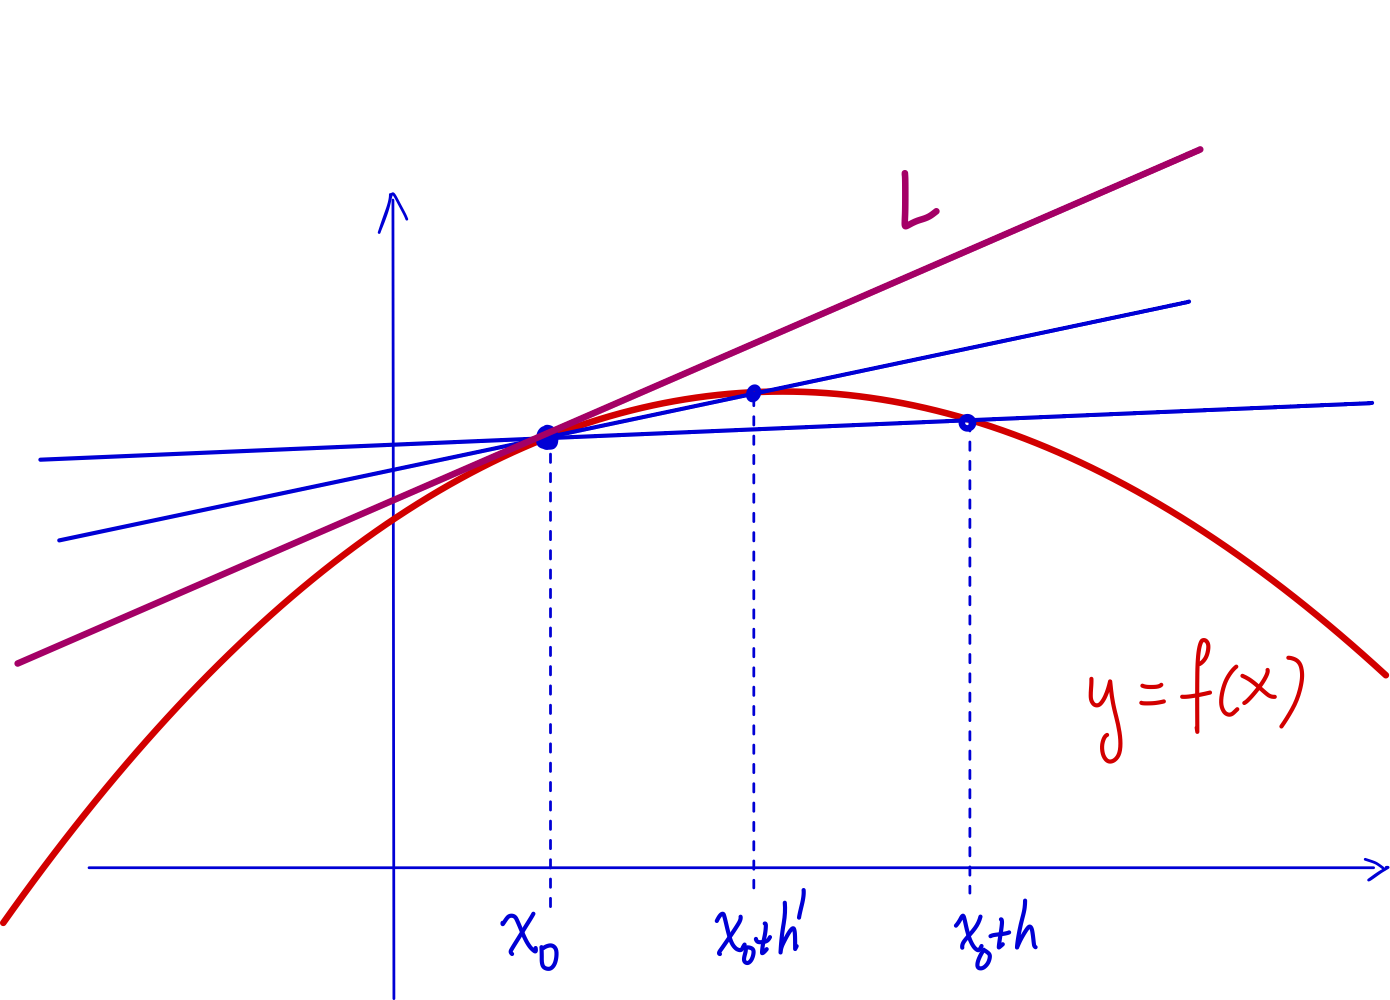
\includegraphics[width=.8\textwidth]{pics/tangente.png}}

Si ahora tomamos límite cuando $h\to 0$, vemos que la recta considerada se va aproximando a la recta $L$ tangente a la curva en el punto de coordenadas $(x_0,f(x_0))$. Por otro lado, $\lim_{h\to 0}m(h)=f'(x_0)$. Deducimos entonces lo siguiente:
\begin{quote}
    Si $f$ es una función definida en $(a,b)$ y existe $f'(x_0)$ para un $x_0\in(a,b)$, entonces $f'(x_0)$ es igual a la pendiente de la recta tangente a la gráfica de $f$ en el punto $(x_0,f(x_0))$.
\end{quote}

La ecuación de la recta tangente $L$ es ahora fácil de encontrar. Tiene pendiente $f'(x_0)$ y pasa por $(x_0,y_0)=(x_0,f(x_0))$:
\[
\frac{y-y_0}{x-x_0} = f'(x_0)
\quad\implies\quad
y - y_0 = f'(x_0)\, (x-x_0).
\]

\begin{example}
    Calculemos la ecuación de la recta tangente a la gráfica de $y=x^2$ en el punto $(x_0,y_0)=(x_0,x_0^2)$, para un $x_0\in\R$ genérico.

    Comenzamos calculando la pendiente de dicha recta, que es la derivada de $f(x)=x^2$ en $x=x_0$. Repetimos lo que hicimos en el ejemplo anterior, cambiando $2$ por $x_0$:
        \begin{align*}
    f'(x_0) 
    &= \lim_{h\to 0}\frac{f(x_0+h)-f(x_0)}{h}
    = \lim_{h\to 0}\frac{(x_0+h)^2-(x_0)^2}{h}
    = \lim_{h\to 0}\frac{x_0^2+2\, x_0\, h+h^2-x_0^2}{h}
    \\
    &= \lim_{h\to 0}\frac{2\, x_0 \, h+h^2}{h}
    = \lim_{h\to 0}\frac{2\, x_0\, \cancel{h}}{\cancel{h}}+\frac{h^{\cancel{2}}}{\cancel{h}}
    = 2\,x_0+0=2\,x_0.
    \end{align*}
    Es decir, la pendiente de la recta tangente a la gráfica de $y=x^2$ en el punto $(x_0,y_0)=(x_0,x_0^2)$ es $2 x_0$. 
    Por lo tanto, la recta tangente es la que tiene esa pendiente y  pasa por $(x_0,y_0)=(x_0,x_0^2)$:
    \[
    \frac{y-y_0}{x-x_0} = 2\, x_0
    \quad\implies\quad
    y - y_0 = 2 \, x_0\, (x-x_0)
    \quad\implies\quad
    y = x_0^2+2 \, x_0\, (x-x_0).
    \]
\end{example}

En el ejemplo anterior vimos que $f(x)=x^2$ tiene derivada en cualquier punto $x_0\in\R$ y que $f'(x_0)=2x_0$ o lo que es lo mismo, $f'(x)=2x$, para todo \xiR.



Esto no es así para todas las funciones, por ejemplo, la función \emph{valor absoluto} no es derivable en $x_0=0$.

\begin{example}
    Consideremos $f(x)=|x|$ y veamos si es derivable en $x_0=0$.
    \begin{align*}
        \lim_{h\to 0} \frac{|0+h|-|0|}h
        =
        \lim_{h\to 0} \frac{|h|}h.
    \end{align*}
    Pero 
    \[
        \lim_{h\to 0^+} \frac{|h|}h
        = \lim_{h\to 0^+} \frac{h}h = 1
        \qquad\text{y}\qquad
        \lim_{h\to 0^-} \frac{|h|}h
        = \lim_{h\to 0^-} \frac{-h}h = -1.
    \]
    Por lo tanto no existe $\lim_{h\to 0} \frac{|0+h|-|0|}h$ y $f(x)=|x|$ no es derivable en $x_0=0$.

    ?`Cuál es la recta tangente al gráfico de $y=|x|$ en el origen $(0,0)$? ?`Existe?

    Aunque sí es diferenciable en $x_0$ si $x_0\neq 0$.
    Queda como ejercicio verificar que
    \[
    f'(x_0) = \begin{cases}
        1,\quad&\text{si $x_0>0$},\\
        -1,\quad&\text{si $x_0<0$}.
        \end{cases}
    \]
\end{example}

La derivada tiene también una interpretación física que es importante destacar. Para establecerla, consideraremos un cuerpo desplazándose sobre una línea recta, por ejemplo, un automóvil en un tramo recto de una ruta.

Fijando una unidad de medida para las longitudes (por ejemplo, el kilómetro) y una unidad de medida para el tiempo (por ejemplo, la hora), entonces la velocidad de dicho automóvil estará medida (en kilómetros por hora) por el cociente entre el espacio que haya recorrido y el tiempo que haya empleado en recorrerlo.

Eso, desde luego, mide una velocidad promedio, pues, en el intervalo de tiempo considerado, el móvil puede haber recorrido algunas partes del trayecto más rápido que otras o, incluso, haberse detenido un rato.
Pero hay una noción de velocidad que no es un promedio, que es una noción de \emph{velocidad instantánea}, y es la que marca el velocímetro.

Independientemente de cual sea el mecanismo por el cual el velocímetro marca la velocidad en cada instante, hay una manera de llegar (teóricamente) a medir velocidades instantáneas a partir de velocidades promedio: si podemos establecer qué posición ocupa el móvil en cada instante, entonces tenemos la distancia recorrida, digamos $s$, en función del tiempo, $s=s(t)$.

Para calcular la velocidad en el instante $t_0$, comenzamos considerando un tiempo $t$ a partir de $t_0$ y calculamos la velocidad promedio entre $t_0$ y $t_0+t$:
\[
\frac{\text{distancia}}{\text{tiempo}}
=\frac{s(t_0+t)-s(t_0)}{t_0+t-t_0}
=\frac{s(t_0+t)-s(t_0)}{t}.
\]
Ahora, para calcular la velocidad en el instante $t_0$, tomamos límite en esta expresión cuando $t\to 0$. Lo que obtenemos es
\[
s'(t_0) = \lim_{t\to t_0}\frac{s(t_0+t)-s(t_0)}{t}.
\]
Deducimos entonces:
\begin{quote}
    Si, en un movimiento rectilíneo, tenemos el espacio recorrido en función del tiempo $s=s(t)$, entonces la velocidad del móvil en el instante $t_0$ está dada por la derivada de dicha función en $t_0$, es decir $s'(t_0)$.
\end{quote}

Las interpretaciones geométricas y física de la derivada tienen una notable importancia en las respectivas disciplinas, pero en este apunte sólo discutiremos (más adelante) unas pocas consecuencias geométricas, dejando el resto para los correspondientes cursos de geometría y física.

Antes de pasar a estudiar propiedades de las funciones derivables, notemos que 
\[
\lim_{h\to 0} \frac{f(x_0+h)-f(x_0)}{h}
= 
\lim_{x\to x_0} \frac{f(x)-f(x_0)}{x-x_0},
\]
que se deduce usando el cambio de variables $x=x_0+h$.

\subsection*{Definición alternativa (pero equivalente) de derivada}

Observemos que, por propiedades de límites tenemos las siguientes equivalencias:
\begin{align*}
f'(x_0) = \lim_{h\to 0} \frac{f(x_0+h)-f(x_0)}{h}
&\quad\iff\quad
f'(x_0) - \lim_{h\to 0} \frac{f(x_0+h)-f(x_0)}{h} = 0
\\
&\quad\iff\quad
\lim_{h\to 0} \bigg[f'(x_0) - \frac{f(x_0+h)-f(x_0)}{h} \bigg]= 0
\\
&\quad\iff\quad
\lim_{h\to 0} \frac{f'(x_0)\cdot h - \big(f(x_0+h)-f(x_0)\big)}{h}= 0
\\
&\quad\iff\quad
\lim_{h\to 0} \frac{f(x_0+h) - f(x_0) - f'(x_0)\cdot h}{h}= 0
\\
&\quad\iff\quad
f(x_0+h) - f(x_0) - f'(x_0)\cdot h= o(h).
\end{align*}
Es decir, $f'(x_0)$ es el número real que cumple que
\[
f(x_0+h) = f(x_0) + f'(x_0) \, h + o(h).
\]
Más precisamente
\begin{quote}
    $f$ es derivable o diferenciable en $x_0$ si existe un número que denotamos $f'(x_0)$ para el que se cumple que 
    \begin{equation}\label{eq:derivada-o(h)}
    f(x_0+h) = f(x_0) + f'(x_0) \, h + o(h).
    \end{equation}
\end{quote}

\begin{example}
    Veamos cómo se calcula la derivada de $f(x)=x^2$ con este método, en un $x_0\in\R$:
    \begin{align*}
        f(x_0+h) &= (x_0+h)^2 
        = \underbrace{x_0^2}_{f(x_0)} + \underbrace{2 \, x_0 }_{\text{número}} \, h + \underbrace{h^2}_{o(h)}
        = f(x_0) + \underbrace{2 \, x_0}_{f'(x_0)} \, h + o(h).
    \end{align*}
    Luego $f'(x_0)=2\, x_0$.
\end{example}

\begin{example}
    Veamos cómo se calcula la derivada de $f(x)=x^3$ con este método, en un $x_0\in\R$.
    \begin{align*}
        f(x_0+h) &= (x_0+h)^3 
        = \underbrace{x_0^3}_{f(x_0)} + \underbrace{3 \, x_0^2 }_{\text{número}} \, h + \underbrace{3 \, x_0 \, h^2+ h^3}_{o(h)}
        = f(x_0) + \underbrace{3 \, x_0^2}_{f'(x_0)} \, h + o(h).
    \end{align*}
    Luego $f'(x_0)=3\, x_0^2$.
\end{example}

\paragraph{Derivabilidad vs.\ Continuidad.}

La noción de derivada es \emph{puntual}, hemos definido qué quiere decir que una función es derivable \emph{en un punto $x_0$}.

Tenemos ya otra noción puntual, que es la de \emph{continuidad}. ?`Cómo se relacionan estos conceptos?

\begin{proposition}
    Si una función es derivable en $x_0$, entonces es continua en $x_0$.
\end{proposition}

\begin{proof}
    Si $f$ es diferenciable en $x_0$, entonces existe un número $f'(x_0)$ que cumple
    \[
    f(x_0+h) = f(x_0) + f'(x_0) \, h + o(h).
    \]
    Tomando límite cuando $h\to0$ a ambos lados tenemos que
    \begin{align*}
    \lim_{h\to 0} f(x_0+h) 
    &= \lim_{h\to 0}\big(f(x_0) + f'(x_0) \, h + o(h)\big)
    \\
    &= \lim_{h\to 0}f(x_0) \,+\, \lim_{h\to 0}f'(x_0) \, h \,+\, \lim_{h\to 0}o(h)
    \\
    &= f(x_0)+0+0=f(x_0).
    \end{align*}
    Luego, $\lim_{h\to 0}f(x_0+h)=f(x_0)$, o lo que es lo mismo,
    $\D \lim_{x\to x_0}f(x)=f(x_0)$.
\end{proof}

La recíproca de esta proposición no es cierta. Basta con pensar en la función \emph{valor absoluto}, que es continua en $x_0=0$, pero no es diferenciable en ese punto.

\begin{example}
    Otro ejemplo interesante es el dado por la siguiente función:
    \[
    f(x) = \begin{cases} x \sen \frac1x,\quad&\text{si $x\neq 0$},
    \\
    0, \quad&\text{si $x=0$}.
    \end{cases}
    \]
    Ya vimos en el capítulo anterior que esta función es continua en $x_0=0$ (por el teorema del emparedado).
    Veamos qué ocurre si queremos calcular $f'(0)$:
    \begin{align*}
        f'(0) 
        &= \lim_{x\to 0} \frac{f(x)-f(0)}{x-0}
        = \lim_{x\to 0} \frac{x\,\sen\frac1x - 0}{x}
        \\
        &= \lim_{x\to 0} \frac{x\,\sen\frac1x}{x}
        = \lim_{x\to 0} \sen\frac1x.
    \end{align*}
    También vimos en el capítulo anterior que este límite no existe.
    Luego, no existe $f'(0)$.
\end{example}
\subsubsection*{Ejercicios de la sección~\getcurrentref{chapter}.\getcurrentref{section}}

\begin{enumerate}
\item Calcular las siguientes derivadas usando la definición:
\begin{multicols}{2}
    \begin{enumerate}
        \item $f'(1)$ para $f(x)=2x+3$
        \item $f'(2)$ para $f(x)=3x^2-1$
        \item $f'(4)$ para $f(x)=\sqrt{x}$
        \item $f'(2)$ para $f(x)=1/x$
    \end{enumerate}
\end{multicols}
\item Determinar si la siguiente función es derivable en $x_0=0$:
\[
    f(x) = \begin{cases} x^2 \sen \frac1x,\quad&\text{si $x\neq 0$},
    \\
    0, \quad&\text{si $x=0$}.
\end{cases}
\]
\item Hallar usando la definición, la derivada de $f:(0,+\infty)\to R$ dada por $f(x)=\sqrt{x}$.
Plantear el cociente incremental y multiplicar por \emph{el conjugado}.
\end{enumerate}


\section{La función derivada. Reglas de derivación}

Supongamos que $f$ está definida en un intervalo abierto $(a,b)$ y que es derivable en todos los puntos de $(a,b)$.
Cuando esto ocurre, diremos que \emph{$f$ es derivable en $(a,b)$}.
Para cada $x\in(a,b)$ tenemos una derivada $f'(x)$. De esta manera, tenemos definida una función:
\[
x \to f'(x),
\]
que se llamará \emph{función derivada de $f$} y se indica $f'$.

%\subsection{Reglas de derivación}

Para seguir adelante con el cálculo de derivadas. Necesitamos tres propiedades que nos indican cómo se comporta la derivada frente a las operaciones elementales de funciones: la suma el producto y el cociente.

\begin{proposition}
    Si $f$ es derivable en $x_0$ y $c$ es una constante, entonces $c\, f$ es derivable en $x_0$ y además
    \[
    (c\, f)'(x_0) = c \, f'(x_0).
    \]
    En palabras: \emph{la derivada de una constante por una función es la constante por la derivada de la función}.
\end{proposition}

\begin{proof}
Utilizaremos la definición alternativa dada en~\eqref{eq:derivada-o(h)}.
Llamamos $g(x)=c\, f(x)$ y por la propiedad distributiva, obtenemos
\begin{align*}
    g(x_0+h) &= (c \, f)(x_0+h) = c \, f(x_0+h) 
    \\
    &= c\, \big( f(x_0) + f'(x_0)\cdot h + o(h) \big) 
    \\
    &=  c\, f(x_0) + c\, f'(x_0)\cdot h + c\, o(h)
    \\
    &=  g(x_0) + c\, f'(x_0)\cdot h +  o(h).
\end{align*}    
Por lo tanto $g'(x_0) = c\, f'(x_0)$.
\end{proof}

\begin{example}
    Ya sabemos que la derivada de $x^2$ es $2\, x$, por lo tanto, 
    \[
    \text{la derivada de $5 x^2$ es  $5 \cdot 2 \, x = 10\,  x$.}
    \]
\end{example}

\begin{proposition}
    Si $f$ y $g$ son diferenciables en $x_0$, entonces $f+g$ es diferenciable en $x_0$ y además
    \[
    (f+g)'(x_0) = f'(x_0)+g'(x_0).
    \]
    En palabras: \emph{la derivada de la suma es la suma de las derivadas}.
\end{proposition}

\begin{proof}
Utilizaremos la definición alternativa dada en~\eqref{eq:derivada-o(h)}.
\begin{align*}
    (f+g)(x_0+h) 
    &= f(x_0+h)+g(x_0+h)
    \\
    &= \big[f(x_0)+f'(x_0)\, h + o(h)\big]
    + \big[g(x_0)+g'(x_0)\, h + o(h)\big]
    \\
    &= \big[f(x_0)+g(x_0)\big] +
    \big[f'(x_0)\, h + g'(x_0)\, h\big] 
    + \big[o(h)+ o(h)\big]
    \\
    &= (f+g)(x_0) +
    \big[f'(x_0)+ g'(x_0)\big] \, h
    + o(h).
\end{align*}
Por lo tanto $(f+g)'(x_0) = f'(x_0)+g'(x_0)$.
\end{proof}

\begin{example}
    Ya sabemos que la derivada de $5 \,x^2$ es $10\,x$, y que la de $x^3 = 3\, x^2$.
    Por lo tanto, 
    \[
    \text{la derivada de $5 x^2 + 6 x^3$ es $10 \, x + 6 \cdot 3 \, x^2 = 10 x + 18 x^2$.}
    \]
\end{example}

\begin{proposition}
    Si $f$ y $g$ son derivables en $x_0$, entonces $f\cdot g$ es derivable en $x_0$ y además
    \[
    (f\cdot g)'(x_0) = f'(x_0)\cdot g(x_0)+f(x_0)\cdot g'(x_0).
    \]
\end{proposition}

\begin{proof}
Utilizaremos la definición alternativa dada en~\eqref{eq:derivada-o(h)}.
Por la propiedad distributiva,
\begin{align*}
    (f\cdot g)(x_0+h) 
    ={}& f(x_0+h)\cdot g(x_0+h)
    \\
    ={}& \big[f(x_0)+f'(x_0)\, h + o(h)\big]
    \cdot \big[g(x_0)+g'(x_0)\, h + o(h)\big]
    \\
    ={}& f(x_0)\cdot g(x_0) 
    + f'(x_0)\cdot g(x_0) 
    + \underbrace{o(h) \cdot g(x_0) }_{o(h)}
    \\
    &+ f(x_0) \cdot g'(x_0) \, h
    + \underbrace{f'(x_0) \, h \cdot g'(x_0) \, h}_{o(h)}
    + \underbrace{o(h) \cdot g'(x_0) \, h}_{o(h)}
    \\
    &
    + \underbrace{f(x_0) \cdot o(h)}_{o(h)}
    + \underbrace{f'(x_0) \cdot o(h)}_{o(h)}
    + \underbrace{o(h) \cdot o(h)}_{o(h)}
    \\
    ={}& f(x_0)\cdot g(x_0) 
    + \big[ f'(x_0)\cdot g(x_0)+f(x_0)\cdot g'(x_0) \big] \, h 
    + o(h).
\end{align*}
Por lo tanto $(f\cdot g)'(x_0) = f'(x_0)\cdot g(x_0)+f(x_0)\cdot g'(x_0)$.
\end{proof}

\begin{proposition}
    Si $g$ es diferenciable en $x_0$, y $g(x_0)\neq 0$, entonces $1/g$ es diferenciable en $x_0$ y además
    \[
    \Big(\frac1g\Big)'(x_0) = - \frac{g'(x_0)}{g(x_0)^2}.
    \]
\end{proposition}

\begin{proof}
    Analicemos el cociente incremental:
    \begin{align*}
         % \frac{\frac1g(x_0+h)-\frac1g(x_0)}h
        \frac{\frac1{g(x_0+h)}-\frac1{g(x_0)}}h
        &= \frac1h \, \left[\frac1{g(x_0+h)}-\frac1{g(x_0)}\right]
        = \frac1h \, \frac{g(x_0)-g(x_0+h)}{g(x_0+h)\,g(x_0)}
        \\
        &= \frac1{g(x_0+h)\,g(x_0)} \, \frac{g(x_0)-g(x_0+h)}h
        \\
        &= - \frac1{g(x_0+h)\,g(x_0)} \, \frac{g(x_0+h)-g(x_0)}h.
    \end{align*}
    Recordamos ahora que como $g$ es derivable en $x_0$ es también continua, y por hipótesis, $g(x_0)\neq 0$. 
    Luego, 
    \[
    \limho \frac1{g(x_0+h)\,g(x_0)} = \frac1{g(x_0)\,g(x_0)} = \frac1{g(x_0)^2}. 
    \]
    Además, $\limho \frac{g(x_0+h)-g(x_0)}h = g'(x_0)$.
    Finalmente,
    \[
    \left(\frac1g\right)'(x_0) = \limho \frac{\frac1{g(x_0+h)}-\frac1{g(x_0)}}h = - \frac{g'(x_0)}{g(x_0)^2}.
    \qedhere
    \]
\end{proof}

Combinando este último resultado con la regla para el producto, obtenemos la regla de derivación para el cociente:

\begin{corollary}
    Si $f$ y $g$ son derivables en $x_0$, y $g(x_0)\neq 0$, entonces $f/ g$ es derivable en $x_0$ y además
    \[
    \left(\frac f g\right)'(x_0) = \frac{f'(x_0)\cdot g(x_0)-f(x_0)\cdot g'(x_0)}{g(x_0)^2}.
    \]
\end{corollary}

\begin{proof}
Como $\D\frac fg = f \cdot \frac1g$ tenemos que
    \begin{align*}
        \left(\frac f g\right)'(x_0) 
        &= \left(f \cdot \frac 1 g\right)'(x_0)
        = f'(x_0) \left(\frac 1 g\right)(x_0) + f(x_0) \left(\frac 1 g\right)'(x_0).
    \end{align*}
Como $g$ es derivable en $x_0$ y $g(x_0)\neq 0$, tenemos que $\left(\frac1g\right)'(x_0) = - \frac{g'(x_0)}{g(x_0)^2}$ y entonces
    \begin{align*}
        \left(\frac f g\right)'(x_0) 
        &= f'(x_0) \frac 1 {g(x_0)} + f(x_0) \left(- \frac{g'(x_0)}{g(x_0)^2}\right)
        = \frac{f'(x_0)\cdot g(x_0)-f(x_0)\cdot g'(x_0)}{g(x_0)^2}.
        \qedhere
    \end{align*}
\end{proof}

Podemos resumir los últimos resultados de la siguiente manera:
\[
(c\, f)' = c\, f',
\qquad
(f+g)' = f'+g',
\qquad
(f\cdot g)' = f'g+f g',
\qquad
\left(\frac f g\right)' = \frac{f'g-f g'}{g^2},
\]
donde la última fórmula tiene sentido en los puntos $x$ donde $g(x)\neq 0$.
Es importante observar que si bien la derivada de la suma es la suma de las derivadas, no es cierto que la derivada del producto es el producto de las derivadas, ni que la derivada del cociente es el cociente de las derivadas.

\paragraph{Notación de Leibniz.}
Otra manera muy usual de denotar a las derivadas es la siguiente, conocida como notación de Leibniz:
\[
f'(x)= \frac{df(x)}{dx}, \qquad\text{o también}\quad f'= \frac{df}{dx}.
\]
Si estamos pensando que $y=f(x)$, es decir, $y$ es la variable \emph{dependiente}, definida como $f(x)$, entonces también suele escribirse
\[
f'(x) = \frac{dy}{dx}.
\]
Esta forma es muy útil cuando uno quiere representar la derivada de una función \emph{anónima}, es decir una función que no tiene nombre asignado. Por ejemplo:
\[
\frac{d (x^2)}{dx} = 2x,
\qquad
\frac{d (5 \, x^2)}{dx} = 5 \frac{d (x^2)}{dx} =5\cdot 2x = 10x.
\]

Con la notación de Leibniz, las reglas de derivación recién presentadas pueden escribirse de la siguiente forma:
\[
\frac{d(c\, f)}{dx} = c\, \frac{df}{dx},
\quad
\frac{d(f+g) }{dx} = \frac{d f}{dx}+\frac{d g}{dx},
\quad
\frac{d(f\cdot g)}{dx} = \frac{df}{dx}g+f \frac{dg}{dx},
\quad
\frac{d\big(\frac f g\big)}{dx} = \frac{\frac{df}{dx}g-f \frac{dg}{dx}}{g^2}.
\]

Finalizamos esta sección aprovechando la regla del producto para saber cuál es la derivada de $f(x) = x^n$ para $n\in\N$.
El caso $n=1$ nos da $f(x)=x$ y $f'(x)=1$, es decir $\frac{dx}{dx}=1$. El caso $n=2$ nos da $\frac{d(x^2)}{dx}=2x$, el caso $n=3$ nos da $\frac{d(x^3)}{dx}=3x^2$. En el caso general, para $n\in\N$, la derivada de $x^n$ será $$\frac{d(x^n)}{dx}=n x^{n-1}$$ y lo vamos a probar por inducción. Ya hemos probado el caso $n=1$ (y también los casos $n=2$ y $n=3$). Supongamos que esta fórmula es válida para un cierto natural $n$ y veamos si es cierta para $n+1$. Observamos que $x^{n+1} = x^n \cdot x$, y utilizando la regla del producto:
\[
\frac{d(x^{n+1})}{dx}
=
\frac{d(x^n\cdot x)}{dx}
= 
\frac{d(x^n)}{dx} x + x^n \frac{dx}{dx}.
\]
Por la hipótesis inductiva, $\frac{d(x^n)}{dx}=n\, x^{n-1}$, así que
\[
\frac{d(x^{n+1})}{dx}
= n\, x^{n-1} \, x + x^n \cdot 1
= n x^n + x^n = (n+1)x^n.
\]

Por lo tanto, todas las funciones polinomiales son derivables, y más aún, 
\begin{multline*}
\text{Si }p(x) = a_n \, x^n + a_{n-1} \, x^{n-1} + \dots + a_2 \, x^2 + a_1 \, x + a_0
\\
\quad\text{\ \ entonces \ \ }
p'(x) = n\, a_n \, x^{n-1} + (n-1) \, a_{n-1} \, x^{n-2} + \dots + 2\, a_2 \, x + a_1.
\end{multline*}

Y por la regla del cociente, también todas las funciones racionales son derivables en todo punto de su dominio (todos los puntos donde el denominador no se anula).


\subsection*{Derivadas de orden superior.}
Como vimos al principio de esta sección, si una función $f$ es derivable, podemos formar una nueva función $f'$, la derivada de $f$. Si $f'$ es a su vez derivable, podemos tomar su derivada $(f')'$, llamada \emph{derivada segunda de $f$} y se designa por $f''$. Si esta función es derivable, podemos volver a calcular su derivada, que será la derivada tercera y se denotará $f'''$, etc. Para derivadas de orden superior a $3$, denotaremos el orden de las derivadas con un supra-índice entre paréntesis. Por ejemplo, la derivada cuarta es $f^{(4)}$, y la $n$-ésima es $f^{(n)}$.
Por ejemplo, si $f(x)=x^5$, tenemos que
\[
f'(x)=5\,x^4,\quad
f''(x)=20\,x^3,\quad
f'''(x)=60\,x^2,\quad
f^{(4)}(x)=120\,x,\quad
f^{(5)}(x)=120,
\]
y $f^{(6)}(x)=0$, con $f^{(n)}(x)=0$, para todo $n\ge 6$.

También podemos usar la notación de Leibniz para las derivadas de orden superior. Si $y=x^5$,
\[
\dd{y}{x}=5\,x^4,\quad
\dd[2]{y}{x}=20\,x^3,\quad
\dd[3]{y}{x}=60\,x^2,\quad
\dd[4]{y}{x}=120\,x,\quad
\dd[5]{y}{x}=120,\quad
\]
con $\D\dd[n]{f}{x}=0$, para todo $n\ge 6$.




\subsubsection*{Ejercicios de la sección~\getcurrentref{chapter}.\getcurrentref{section}}

\begin{enumerate}
\item Hallar $f'(x)$ siendo $f(x)$ igual a:
\begin{multicols}{2}
\begin{enumerate}
    \item $\D 3x^3+6x^2-2x+1$
    \item $\D x(3+x^2)$
    \item $\D 4x(2+x^3+5x^4)$
    \item $\D (x+2)(x+3)(3x+1)(2+5x^2)$
    \item $\D \frac{x-1}x$
    \item $\D \frac{4x-3}{2x+4}$
    \item $\D \frac{(x+3)^2(4x-1)}{(2x+1)^2(3x-2)}$
    \item $\D \frac{x^3}{(4-x^2)^2}$
    \item $\D 4x-\frac2x$
\end{enumerate}
\end{multicols}

\item Calcular las siguientes derivadas:
\begin{multicols}{2}
\begin{enumerate}
    \item $\D \dd[3]{}{x} \big(3x^3+6x^2-2x+1\big)$
    \item $\D \dd[4]{}{x}\big(x(3+x^2)\big)$
    \item $\D \dd[2]{}{x}\big((x+2)(x+3)(3x+1)(2+5x^2)\big)$
    \item $\D \dd[2]{}{x}\frac{x-1}x$
\end{enumerate}
\end{multicols}

\item Sea $f(x)=x^n$, para \niN. Hallar $f^{(k)}(x)$, para
\begin{multicols}{3}
    \begin{enumerate}
    \item $k=n$;
    \item $k>n$;
    \item $k<n$.
\end{enumerate}
\end{multicols}

\item Dada la función polinómica $\D p(x)=a_n x^n + a_{n-1} x^{n-1} + \dots + a_1 x + a_0$:
\begin{multicols}{2}
    \begin{enumerate}
    \item Hallar $\D \dd[n]{p(x)}{x}$;
    \item Hallar $\D \dd[k]{p(x)}{x}$, para $k>n$.
\end{enumerate}
\end{multicols}


\end{enumerate}


\section{Ejemplos importantes}

La potencia del Cálculo Diferencial en sus diversas aplicaciones depende del hecho siguiente: es muy fácil probar que casi todas las funciones hasta aquí estudiadas (polinómicas, trigonométricas, logarítmicas, etc.) son derivables en todo su dominio, y es muy fácil encontrar sus funciones derivadas. Veamos cómo.

\begin{example}
    Consideremos la función constante $f(x)=c$, para todo \xiR. Su derivada es la función nula. En efecto, para \xiR,
    \[
    \frac{f(x+h)-f(x)}{h} = \frac{c-c}h = \frac0h = 0,\ \ \forall h\neq 0
    \quad\implies\quad
    \lim_{h\to0}\frac{f(x+h)-f(x)}{h} = 0.
    \]
\end{example}

\begin{example}
    La derivada de la función identidad $f(x)=x$ es también fácil de encontrar.  En efecto, para \xiR,
    \[
    \frac{f(x+h)-f(x)}{h} = \frac{x+h-x}h = \frac hh = 1,\ \ \forall h\neq 0
    \quad\implies\quad
    \lim_{h\to0}\frac{f(x+h)-f(x)}{h} = 1.
    \]
    Luego, para la función identidad $f(x)=x$, resulta $f'(x)=1$.
\end{example}

\begin{example}
    Ya vimos que la derivada de $f(x)=x^2$ es $f'(x)=2x$, y que la derivada de $g(x)=x^3$ es $g'(x)=3x^2$.
\end{example}

\begin{example}
    Consideremos ahora un ejemplo un poquito más complicado, que es el de la función \emph{seno}.
    Utilizaremos ahora la identidad trigonométrica que dice que
    \[
    \sen(a)-\sen(b) = 2 \cos\big(\frac{a+b}2\big) \sen\big(\frac{a-b}2\big), 
    \quad\text{para todo $a,b\in\R$}.
    \]
    Sea $f(x)=\sen(x)$. Planteamos el cociente incremental 
    \begin{align*}
        \lim_{h\to0} \frac{f(x+h)-f(x)}{h} 
        &= 
        \lim_{h\to0} \frac{\sen(x+h)-\sen(x)}{h} 
        = 
        \lim_{h\to0} \frac{2\cos\big(\frac{x+h+x}2\big)\sen\big(\frac{x+h-x}2\big)}{h} 
        \\
        &= 
        \lim_{h\to0} \cos\big(\frac{2x+h}2\big)\frac{2\sen\big(\frac{h}2\big)}{h} 
        = 
        \lim_{h\to0} \cos\big(x+\frac{h}2\big)\frac{\sen\big(\frac{h}2\big)}{h/2} 
        \\
        &= 
        \lim_{h\to0} \cos\big(x+\frac{h}2\big) \lim_{h\to0}  \frac{\sen\big(\frac{h}2\big)}{h/2} 
        = \cos(x) \cdot 1 = \cos (x),
    \end{align*}
    donde hemos utilizado que la función coseno es continua (que implica $\lim_{h\to 0}\cos(x+\frac h2)=\cos(x)$), y que $\lim_{y\to0}\sen(y)/y=1$.
    Por lo tanto, la derivada de la función $f(x)=\sen(x)$ es $f'(x)=\cos(x)$.
\end{example}

\begin{example}
    Veamos ahora cuál es la derivada de la función \emph{coseno}.
    Utilizaremos ahora la identidad trigonométrica que dice que
    \[
    \cos(a)-\cos(b) = -2 \sen\big(\frac{a+b}2\big) \sen\big(\frac{a-b}2\big), 
    \quad\text{para todo $a,b\in\R$}.
    \]
    Sea $f(x)=\cos(x)$. Planteamos el cociente incremental:
    \begin{align*}
        \lim_{h\to0} \frac{f(x+h)-f(x)}{h} 
        &= 
        \lim_{h\to0} \frac{\cos(x+h)-\cos(x)}{h} 
        =
        \lim_{h\to0} \frac{-2 \sen\big(\frac{x+h+x}2\big) \sen\big(\frac{x+h-x}2\big)}h
        \\
        &= 
        \lim_{h\to0} -\sen\big(x+\frac h2\big) \frac{\sen\big(\frac h2\big)}{h/2}
        = 
        -\lim_{h\to0} \sen\big(x+\frac h2\big) \lim_{h\to0} \frac{\sen\big(\frac h2\big)}{h/2}
        \\
        &= -\sen(x) \cdot 1 = -\sen(x),
    \end{align*}
    donde hemos utilizado que la función seno es continua (que implica $\lim_{h\to 0}\sen(x+\frac h2)=\sen(x)$), y nuevamente que $\D\lim_{y\to0}\sen(y)/y=1$.
    Por lo tanto, la derivada de la función $f(x)=\cos(x)$ es $f'(x)=\sen(x)$.
\end{example}

\begin{example}
    Consideremos ahora la función logaritmo natural $f(x)=\ln x$, con dominio $(0,+\infty)$. Planteamos el cociente incremental:
    \begin{align*}
        \frac{f(x+h)-f(x)}{h} 
        &= 
        \frac{\ln(x+h)-\ln(x)}h
        =
        \frac{\ln\big(\frac{x+h}x\big)}h
        =
        \frac1h \ln\big(\frac{x+h}x\big)
        \\
        &= 
        \ln \big(\frac{x+h}x\big)^{1/h}
        = \ln \big(1+\frac{h}{x}\big)^{1/h}
        = \ln \big(1+\frac{1}{x/h}\big)^{1/h}
        \\
        &= \ln\bigg( \big(1+\frac{1}{x/h}\big)^{x/h} \bigg)^{1/x}
        = \frac1x \ln \big(1+\frac{1}{x/h}\big)^{x/h}.
    \end{align*}        
    Ahora bien, con el cambio de variables $y=\frac xh$, como $\lim_{h\to 0}y = \infty$,
    \[
    \lim_{h\to 0} \big(1+\frac{1}{x/h}\big)^{x/h} 
    = \lim_{y\to\infty} \big(1+\frac{1}{y}\big)^{y}
    = e.
    \]
    Por lo tanto, $\lim_{h\to 0} \ln \big(1+\frac{1}{x/h}\big)^{x/h} =\ln e = 1$ y finalmente
    \[
    \lim_{h\to0}  \frac{\ln(x+h)-\ln(x)}h
        = \frac1x \cdot 1 = \frac1x.
    \]
    Es decir, la derivada de la función logaritmo natural $f(x)=\ln x$ es $\D f'(x)=\frac1x$.
\end{example}

\begin{example}
    Por último, estudiemos la derivada de la función exponencial $f(x)=e^x$.
     Planteamos el cociente incremental:
    \begin{align*}
        \frac{f(x+h)-f(x)}{h} 
        &= \frac{e^{x+h}-e^x}h
        = \frac{e^x \, e^h-e^x}h
        = \frac{e^x \big(e^h-1\big)}h
        = e^x \frac{e^h-1}h.
    \end{align*}
    Tenemos entonces que calcular $\limho \frac{e^h-1}h$. Hacemos el cambio de variable $y=e^h-1$ y observamos, por un lado, que $$\limho\, y = \limho (e^h-1) = e^0-1=1-1=0.$$
    Por otro lado, si $y=e^h-1$, entonces $e^h=1+y$ y $h=\ln(1+y)$. Luego,
    \begin{align*}
        \limho \frac{e^h-1}h 
        = \lim_{y\to0} \frac{y}{\ln(1+y)}
        = \lim_{y\to0} \frac{1}{\frac1y\ln(1+y)}
        = \lim_{y\to0} \frac{1}{\ln(1+y)^{1/y}}.
    \end{align*}
    Como vimos recién, $\lim_{y\to 0} (1+y)^{1/y}=e$, por lo que 
    $\lim_{y\to 0} \ln (1+y)^{1/y}=\ln e=1$, y finalmente
    \[
    \limho  \frac{e^{x+h}-e^x}h
    = e^x \limho \frac{e^h-1}h 
    = e^x \lim_{y\to0} \frac{1}{\ln(1+y)^{1/y}}
    = e^x \cdot 1 = 1.
    \]
    Es decir, la derivada de la función exponencial $f(x)=e^x$ es $f'(x)=e^x$.
\end{example}

Podemos resumir los resultados anteriores de la siguiente manera:

\noindent\hfil
\begin{minipage}{.4\textwidth}
\def\arraystretch{1.8}
\begin{tabular}{|c|c|}
    \hline
    $f(x)$ & $f'(x)$ \\
    \hline\hline
    $\D c$ (constante) 
    & $\D 0$
    \\ \hline
    $\D x^n$ 
    & $\D nx^{n-1}$
    \\ \hline
    $\D \sen x$ 
    & $\D \cos x$
    \\ \hline
    $\D \cos x$ 
    & $\D -\sen x$
    \\ \hline
    $\D \ln x$ 
    & $\D \frac1x$
    \\ \hline
    $\D e^x$ 
    & $\D e^x$
    \\ \hline
\end{tabular}
\end{minipage}
\hfil
\begin{minipage}{.4\textwidth}
\begin{align*}
    \frac{dc}{dx} &= 0 \\[5pt]
    \frac{d(x^n)}{dx} &= n x^{n-1}\\[5pt]
    \frac{d\sen x }{dx } &= \cos x  \\[5pt]
    \frac{d \cos x}{dx } &= -\sen x  \\[5pt]
    \frac{d\ln x }{dx } &=  \frac1x \\[5pt]
    \frac{d e^x}{dx } &= e^x
\end{align*}
\end{minipage}

Es importante notar que el procedimiento que nos llevó a las fórmulas de la tabla precedente, por un lado demuestra que todas las funciones consideradas son derivables en todo punto de su dominio, y por otro lado nos dice explícitamente cuánto valen sus derivadas en cualquier punto.

\subsubsection*{Ejercicios de la sección~\getcurrentref{chapter}.\getcurrentref{section}}

\begin{enumerate}
\item Hallar $f'(x)$ siendo $f(x)$ igual a:
\begin{multicols}{2}
\begin{enumerate}
    \item $\D \tan x$
    \item $\D \cotan x$
    \item $\D \sec x$
    \item $\D \cosec x$
    \item $\D \frac{x+e^x}{5-x^2}+\tan x$
    \item $\D x \ln x$
\end{enumerate}
\end{multicols}

\item Se definen las funciones hiperbólicas de la siguiente manera:
\[
\cosh x = \frac{e^x+e^{-x}}{2},
\qquad
\senh x = \frac{e^x-e^{-x}}{2}
\]
\begin{enumerate}
    \item Probar que $\cosh^2 x-\senh^2 x = 1$
    \item Probar que $\D\dd{\senh x}{x} = \cosh x$
    \item Probar que $\D\dd{\cosh x}{x} = \senh x$
\end{enumerate}

\item Hallar una fórmula para la derivada de $\log_a x$.

\item Hallar las siguientes derivadas:
\begin{multicols}{2}
    \begin{enumerate}
        \item $\D\dd[2]{\sen x}{x}$
        \item $\D\dd[2]{\cos x}{x}$
        \item $\D\dd[2]{\senh x}{x}$
        \item $\D\dd[2]{\cosh x}{x}$
    \end{enumerate}
\end{multicols}


\item Hallar las siguientes derivadas, para \niN:
\begin{multicols}{2}
    \begin{enumerate}
        \item $\D\dd[n]{\sen x}{x}$
        \item $\D\dd[n]{\cos x}{x}$
        \item $\D\dd[n]{\senh x}{x}$
        \item $\D\dd[n]{\cosh x}{x}$
    \end{enumerate}
\end{multicols}
\end{enumerate}


\section{Regla de la cadena}

La regla de la cadena es la regla que nos permite derivar la composición de funciones.

\begin{proposition}[Regla de la cadena]
Supongamos que $g$ es derivable en $x_0$ y que $f$ es derivable en $y_0 = g(x_0)$.
Entonces $f\circ g$ es derivable en $x_0$ y
\[
(f\circ g)'(x_0) = f'(y_0) \cdot g'(x_0).
\]
\end{proposition}

\begin{proof}
Como $f$ es derivable en $y_0 = g(x_0)$, tenemos que
\[
f(y_0+k) = f(y_0) + f'(y_0) \cdot k + o(k).
\]
Como $g$ es derivable en $x_0$, tenemos que 
\[
g(x_0+h) = g(x_0) + g'(x_0) \cdot h + o(h).
\]
Luego
\begin{align*}
    f\circ g(x_0+h) 
    &= f\big(g(x_0+h)\big) \\
    &= f\big(g(x_0)+\underbrace{g'(x_0)[h]+o(h)}_k \big) \\
    &= f\big(y_0 +\underbrace{g'(x_0)[h]+o(h)}_k \big) \\
    &= f(y_0) + f'(y_0) \big[\underbrace{g'(x_0)h+o(h)}_k\big] + o(\underbrace{g'(x_0)h+o(h)}_k)
    \\
    &= f(y_0) + f'(y_0) \big[g'(x_0)h\big] +
        \underbrace{f'(y_0)\big[o(h)\big] + o(g'(x_0)h+o(h))}_{o(h)}.
\end{align*}
Luego
\begin{align*}
    f\circ g(x_0+h) &= f\circ g(x_0) + f'(y_0) \big[g'(x_0)h\big] + o(h)\\
     &= f\circ g(x_0) + f'(y_0) g'(x_0) \big[h\big] + o(h).
\end{align*}
Por lo tanto
\[
(f\circ g)'(x_0) = f'(y_0)\, g'(x_0) = f'\big(g(x_0)\big) \, g'(x_0).
\qedhere
\]
\end{proof}

\begin{comment}
Demostración con la definición alternativa.
\begin{align*}
    f\big(g(x+{\delta x})\big) &= f\big(g(x)+\underbrace{g'(x)[{\delta x}]+o({\delta x})}_{\delta g} \big) \\
    &= f\big(g(x)\big) + f'\big(g(x)\big) \big[\underbrace{g'(x){\delta x}+o({\delta x})}_{\delta g}\big] + o(\underbrace{g'(x){\delta x}+o({\delta x})}_{\delta g})
    \\
    &= f\big(g(x)\big) + f'\big(g(x)\big) \big[g'(x){\delta x}\big] +
    \underbrace{f'\big(g(x)\big)\big[o({\delta x})\big] + o(g'(x){\delta x}+o({\delta x}))}_{o({\delta x})}.
\end{align*}
Luego
\begin{align*}
    f\circ g(x+{\delta x}) &= f\circ g(x) + f'\big(g(x)\big) \big[g'(x){\delta x}\big] + o({\delta x})\\
    &= f\circ g(x) + f'\big(g(x)\big) g'(x) \big[{\delta x}\big] + o({\delta x}).
\end{align*}
Por lo tanto
\[
f\circ g'(x) = f'\big(g(x)\big) g'(x)
\]
\end{comment}

\begin{example}
    Calculemos la derivada de $h(x) = \sen(x^2+x)$. Definimos $y=g(x)=x^2+x$ y $f(y) = \sen(y)$.
    Luego $f'(y)=\cos(y)$ y $g'(x)=2x+1$. Entonces
    \[
    h'(x) = f\circ g'(x) = f'(y) g'(x) = \cos(y)\, (2x+1) = \cos(x^2+x)\, (2x+1).
    \]
    En palabras podemos describir lo que hemos hecho de la siguiente forma:
    como la función es el seno de una expresión, la derivada es el coseno de la expresión, pero multiplicado por la derivada de esa expresión.
\end{example}

\begin{remark}[Regla de la cadena con Notación de Leibniz]
    Notemos que si llamamos $y=g(x)$ y $z=f(y)$, entonces la regla de la cadena $ (f\circ g)'(x_0) = f'(y_0) \cdot g(x_0)$ se escribe
    \[
    \frac{dz}{dx} = \frac{dz}{dy}\cdot \frac{dy}{dx}.
    \]
\end{remark}

\begin{example}
    Consideremos $f:\R\to\R$ dada por $\D f(x)=\ln(1+e^x)$. Calculemos su derivada. Como la derivada de $\ln y = \frac1y$, la derivada de $\ln (1+e^x)$ es $\D \frac1{1+e^x}$ \emph{multiplicada por la derivada de $1+e^x$.} Es decir,
    \[
    f'(x) = \frac1{1+e^x}\cdot (0+e^x) = \frac{e^x}{1+e^x}.
    \]
    Si utilizamos la notación de Leibniz, tenemos:
    \[
    \frac{d \big(\ln (\overbrace{1+e^x)}^y\big)}{dx} 
    = \underbrace{\frac{1}{1+e^x}}_{\frac{d \ln y}{dy}= \frac1y} \cdot \frac{d(1+e^x)}{dx}
    = \frac1{1+e^x}\cdot (0+e^x) = \frac{e^x}{1+e^x}.
    \]
\end{example}

\paragraph{Composición de tres o más funciones.}
Si tenemos la composición de tres o más funciones, aplicamos reiteradamente la regla de la cadena, por ejemplo:
\begin{align*}
 (f\circ g\circ h)'(x_0)
 &= \big[f\circ (g\circ h)\big]'(x_0) 
 = f'(g\circ h(x_0)) \cdot (g\circ h)'(x_0)
 \\
 &= f'(g\circ h(x_0)) \cdot g'(h(x_0)) \cdot h'(x_0).
\end{align*}
Si les asignamos nombres a las variables intermedias, por ejemplo:
\[
u = h(x),\qquad v=g(u),\qquad w=f(v),
\]
entonces $w=(f\circ g\circ h)'(x)$, y 
\[
\frac{dw}{dx} = \frac{dw}{dv} \cdot \frac{dv}{du} \cdot \frac{du}{dx}.
\]

\begin{example}
    Consideremos ahora la función \emph{exponencial} $a^x$ definida para $a>0$ con dominio $\R$. Para calcular la derivada de esta función haremos uso de la identidad $a^x=e^{x \ln a}$ de la siguiente manera:
    \[
    \frac{d \big(a^x\big)}{dx} = \frac{d \big(e^{x \ln a}\big)}{dx}
    = \underbrace{e^{x \ln a}}_{a^x} \cdot \underbrace{\frac{d (x\ln a)}{dx}}_{\ln a \cdot 1}
    = a^x \cdot \ln a
    = \ln a \cdot a^x.
    \]
\end{example}

\begin{example}
    Consideremos ahora la función \emph{potencia} $x^\alpha$ para $\alpha\in\R$, con dominio $(0,+\infty)$. Utilizamos ahora la identidad $x^\alpha=e^{\alpha \ln x}$ de la siguiente manera
    \[
    \frac{d \big(x^\alpha\big)}{dx} = \frac{d \big(e^{\alpha \ln x}\big)}{dx}
    = \underbrace{e^{\alpha \ln x}}_{x^\alpha} \cdot \underbrace{\frac{d (\alpha \ln x)}{dx}}_{\alpha \cdot \frac1x}
    = x^\alpha \cdot \alpha \frac 1x
    = \alpha \, x^{\alpha-1}.
    \]
    Como caso particular, si $\alpha=n\in\N$ volvemos a obtener la fórmula $\D \frac{d \big(x^n\big)}{dx}=n \, x^{n-1}$. Pero ahora la fórmula vale para cualquier potencia, no necesariamente entero, por ejemplo
    \[
    \frac{d \sqrt{x}}{dx} 
    =
    \frac{d \big(x^{1/2}\big)}{dx}
    = \frac12 x^{\frac12-1} 
    = \frac12 x^{-\frac12}
    = \frac12\frac1{\sqrt{x}}
    = \frac1{2\sqrt{x}}.
    \]
\end{example}


\subsubsection*{Ejercicios de la sección~\getcurrentref{chapter}.\getcurrentref{section}}

\begin{enumerate}
\item Hallar $f'(x)$ siendo $f(x)$ igual a:
\begin{multicols}{2}
\begin{enumerate}
    \item $\D \sqrt{2x^2+3}$
    \item $\D \sqrt{6x^2-3x-2}$
    \item $\D (x^2+1)\sqrt{x^2+1}$
    \item $\D \frac{x^3}{(4-x^2)^3}$
    \item $\D \sqrt{x^2+a^2}$
    \item $\D \frac{a^2}{\sqrt{a^2-x^2}}$
    \item $\D \tan \frac{x^2+2x-1}{(x^2+3)^2}$
    \item $\D \sen\big(\sen(\cos x)\big)$
    \item $\D e^{\sen x}+e^{\tan x}$
    \item $x \sen x+\sqrt[3]{x^2}$
    \item $\D \sen(3x^3-1) \, (4x^2+7)$
    \item $\D e^{\sen x} + e^{\tan x}$
    \item $\D x^3\ln x+e^{x^2}$
    \item $\D \frac{\ln(x+2)}{x+2}$
    \item $\D \big(\ln x\big)^3$
    \item $\D \ln (x^3)$
    \item $\D \ln \frac{\sqrt x-\sqrt a}{\sqrt x+\sqrt a}$
    \item $\D \frac{x^3}{\ln x}$
    \item $\D x^{3x}$
    \item $\D (2^x)^x$
    \item $\D (x^2+1)^{\sqrt x}$
    \item $\D x^{x^x}$
\end{enumerate}
\end{multicols}

\end{enumerate}



\section{Teoremas del valor medio y aplicaciones}

En esta sección vamos a ver cómo el conocimiento de la derivada de una función nos puededar información acerca de la función misma. 
Eso no es extraño ya que, según indicamos en la primera sección de este capítulo, la derivada es una medida de la \emph{variación instantánea} de la función. Si uno conoce cómo varía la función, puede deducir propiedades de la función misma.

En primer lugar, recordemos que un punto $x_0$ se llama
\emph{punto máximo} de $f$ si $f(x_0)\ge f(x)$ para todo $x$ en el dominio de $f$.
En otras palabras, un punto máximo de $f$ es un punto en donde $f$ alcanza su máximo. Análogamente, un punto mínimo de $f$ es un punto en donde $f$ alcanza su menor valor posible.

Por ejemplo, si consideramos la función $f(x)=\cos(x)$, entonces el máximo de $f$ es $1$, y tiene infinitos puntos máximos, son todos los $x$ para los cuales $\cos(x)=1$, es decir, $x = 2n\pi$, $n\in\Z$.
Los puntos mínimos de $f$ son aquellos puntos donde $\cos(x)=-1$, es decir $x=\pi+2n\pi$, $n\in\Z$.
Recordemos que $f'(x)=-\sen(x)$, y observemos que $f'(x)=-\sen(x)=0$, para todos los puntos máximos y mínimos de $f$, que son todos los puntos de la forma $n\pi$, $n\in\Z$.

\bigskip
\centerline{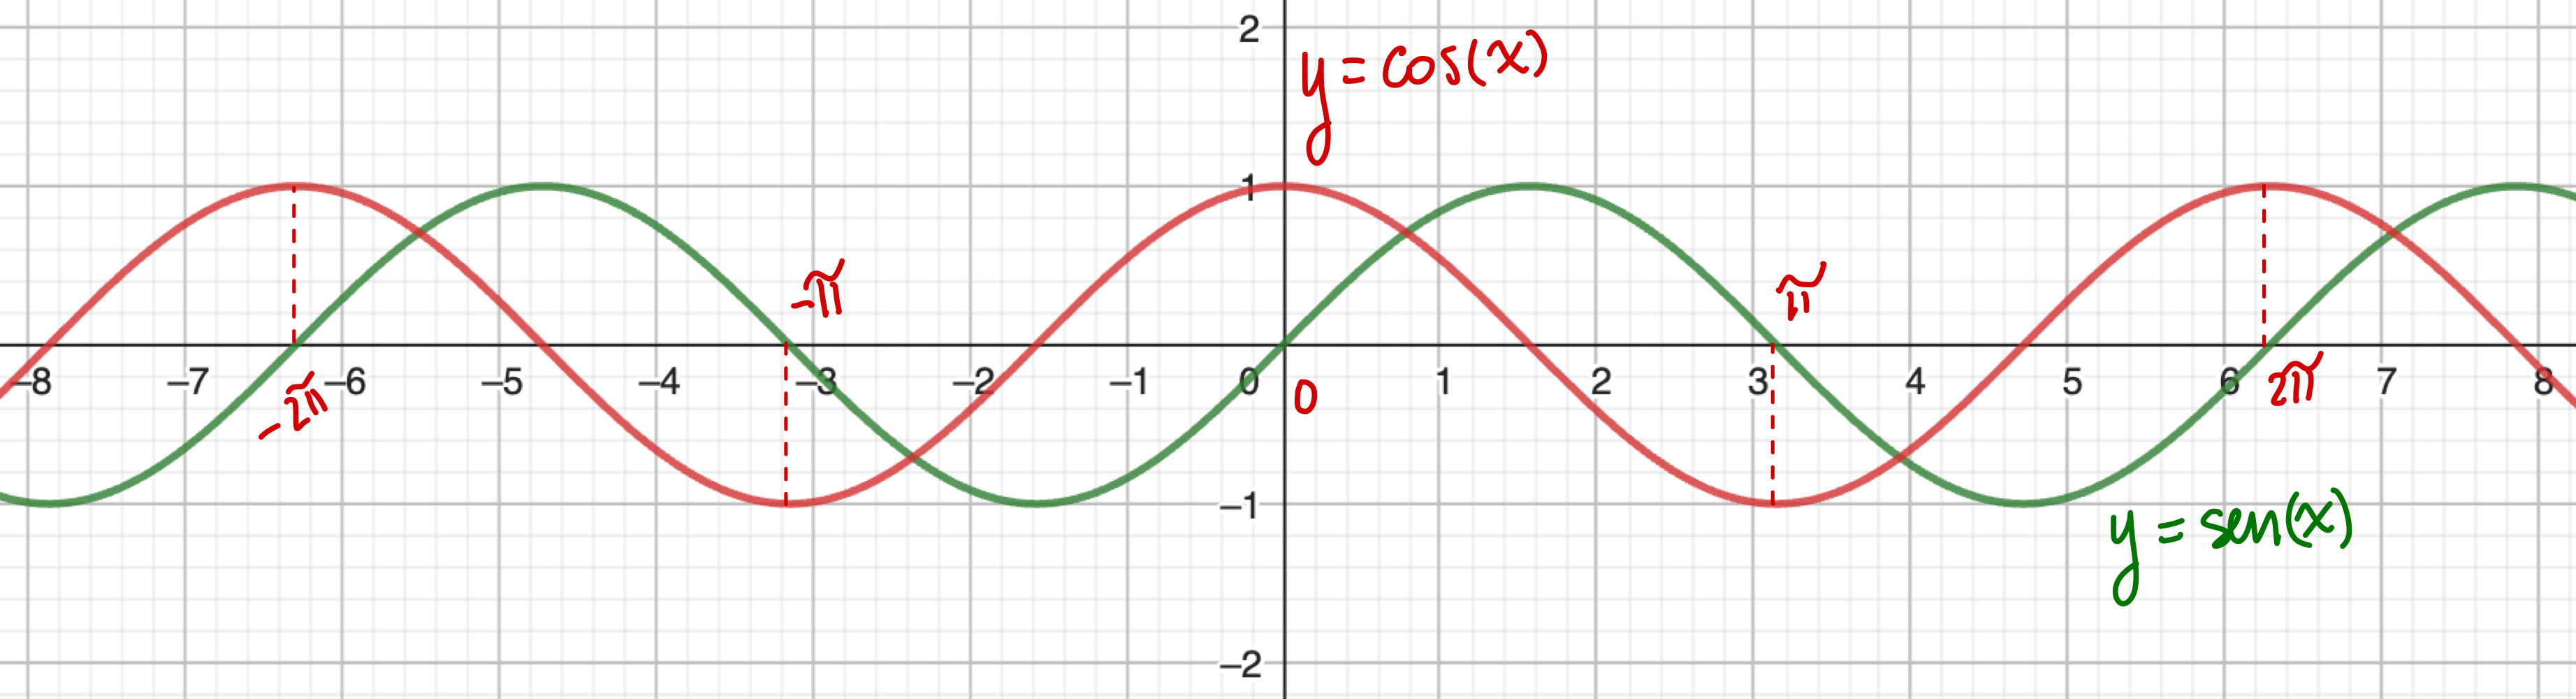
\includegraphics[width=.8\textwidth]{pics/seno-coseno.png}}


Esto que observamos para la función coseno y su derivada, ocurre en general, como lo establece el siguiente teorema.

\begin{theorem}[Teorema de Fermat]
    Si $f$ está definida en el intervalo abierto $(a,b)$ y si $x_0\in(a,b)$ es un punto máximo o un punto mínimo de $f$ donde $f$ es derivable, entonces
    \[
    f'(x_0)=0.
    \]
\end{theorem}

\begin{proof}
    Supongamos que $f$ tiene un mínimo en $x_0$. Entonces
    \[
    f(x)\ge f(x_0), \quad\text{para todo $x\in (a,b)$.}
    \]
    Como $f$ es derivable, existe $\D\limxo \frac{f(x)-f(x_0)}{x-x_0} = f'(x_0)$, y luego
    \[
    f'(x_0) = \limxo \frac{f(x)-f(x_0)}{x-x_0} = \limxop \frac{f(x)-f(x_0)}{x-x_0} = \limxom \frac{f(x)-f(x_0)}{x-x_0}.
    \]
    Si $x>x_0$, entonces $\frac{f(x)-f(x_0)}{x-x_0}\ge 0$ por lo que 
    \[
    f'(x_0) = \limxop \frac{f(x)-f(x_0)}{x-x_0} \ge 0.
    \]
    Si $x<x_0$, entonces $\frac{f(x)-f(x_0)}{x-x_0}\le 0$ por lo que 
    \[
    f'(x_0) = \limxom \frac{f(x)-f(x_0)}{x-x_0} \le 0.
    \]
    Por lo tanto, $0 \le f'(x_0) \le 0$, es decir $f'(x_0)=0$.

    Análogamente se prueba la misma conclusión si $f$ tiene un máximo en $x_0$.
\end{proof}

Observemos que el teorema de Fermat no se puede aplicar si la función está definida sólo sobre un intervalo cerrado $[a,b]$ y alcanza su máximo o mínimo en un extremo.

\medskip
\centerline{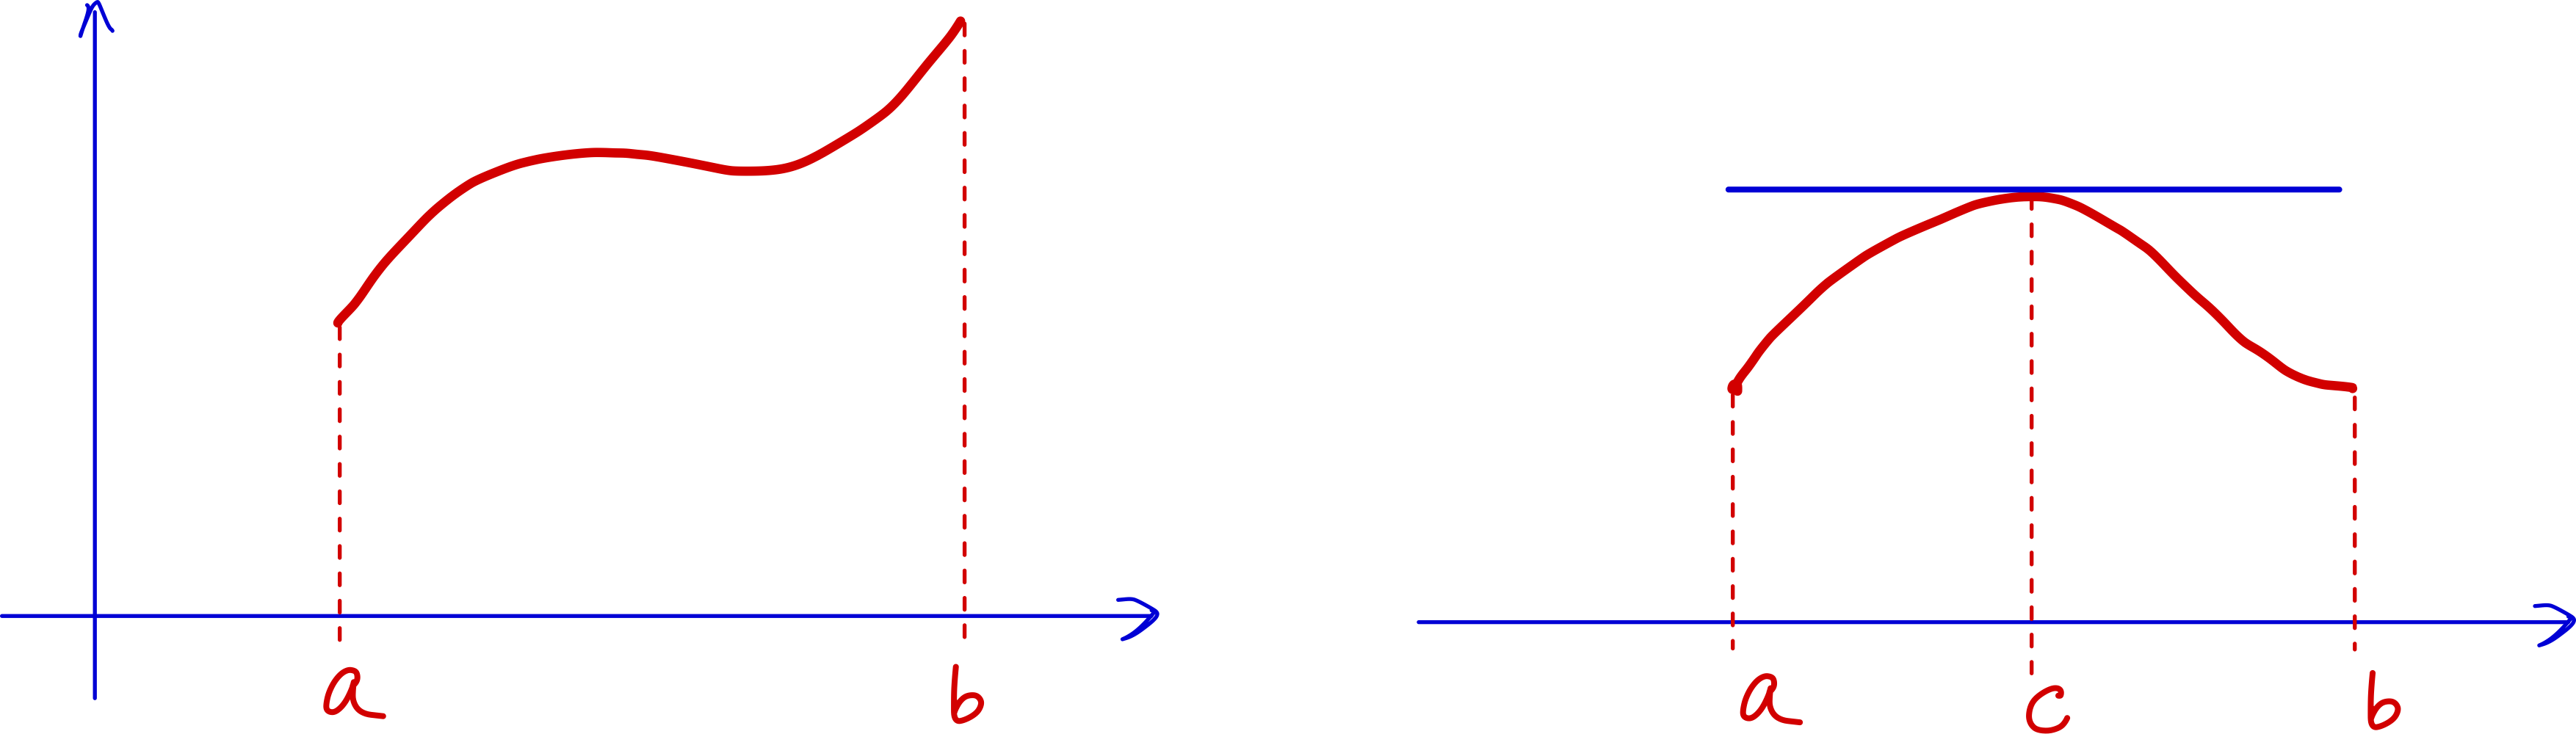
\includegraphics[width=.8\textwidth]{pics/rolle.png}}

Ahora, para funciones definidas en intervalos cerrados, probamos el hecho, geométricamente evidente de que si una función toma el mismo valor en los extremos de un intervalo, entonces, en algún punto intermedio de dicho intervalo, la tangente será horizontal. Más precisamente:

\begin{theorem}[Teorema de Rolle]
    Si $f$ es continua en $[a,b]$, derivable en $(a,b)$ y $f(a)=f(b)$, entonces existe $c\in(a,b)$ tal que $f'(c)=0$.
\end{theorem}

\begin{proof}
    Como $f$ es continua en el intervalo cerrado $[a,b]$, entonces por el Teorema~\ref{T:continua->maximo y minimo} existe $x_1\in[a,b]$ donde $f$ alcanza su mínimo y existe $x_2\in [a,b]$ donde $f$ alcanza su máximo.

Existen diferentes posibilidades:
\begin{itemize}
    \item     Si $x_1\neq a$ y $x_1\neq b$, entonces $x_1\in(a,b)$. Luego, como $f$ es diferenciable en $(a,b)$ y alcanza su mínimo en $x_1\in(a,b)$, el Teorema de Fermat nos dice que $f'(x_1)=0$, y hemos probado el teorema.
    \item  Si $x_2\neq a$ y $x_2\neq b$, entonces $x_2\in(a,b)$. Luego, como $f$ es diferenciable en $(a,b)$ y alcanza su máximo en $x_2\in(a,b)$, el Teorema de Fermat nos dice que $f'(x_2)=0$, y hemos probado el teorema.
    \item Si no ocurre ningúno de los dos casos anteriores, quiere decir que los máximos y mínimos se alcanzan en los extremos del intervalo. Pero en los extremos del intervalo la función toma el mismo valor, luego
    \[
    f(a)=f(b)\le f(x)\le f(a)=f(b), \quad\text{para todo $x\in [a,b]$}.
    \]
    Es decir, la función $f$ es constante en $[a,b]$ y por lo tanto $f'(x)=0$ para todo $x\in(a,b)$.\qedhere
\end{itemize}
\end{proof}

Este fue nuestro primer Teorema del Valor Medio. El segundo, que enunciaremos y probaremos a continuación, tiene también una interpretación geométrica: existe algún punto entre $a$ y $b$ en donde la recta tangente es paralela a la \emph{cuerda} (recta que pasa por $(a,f(a))$ y $(b,f(b))$.

\medskip
\centerline{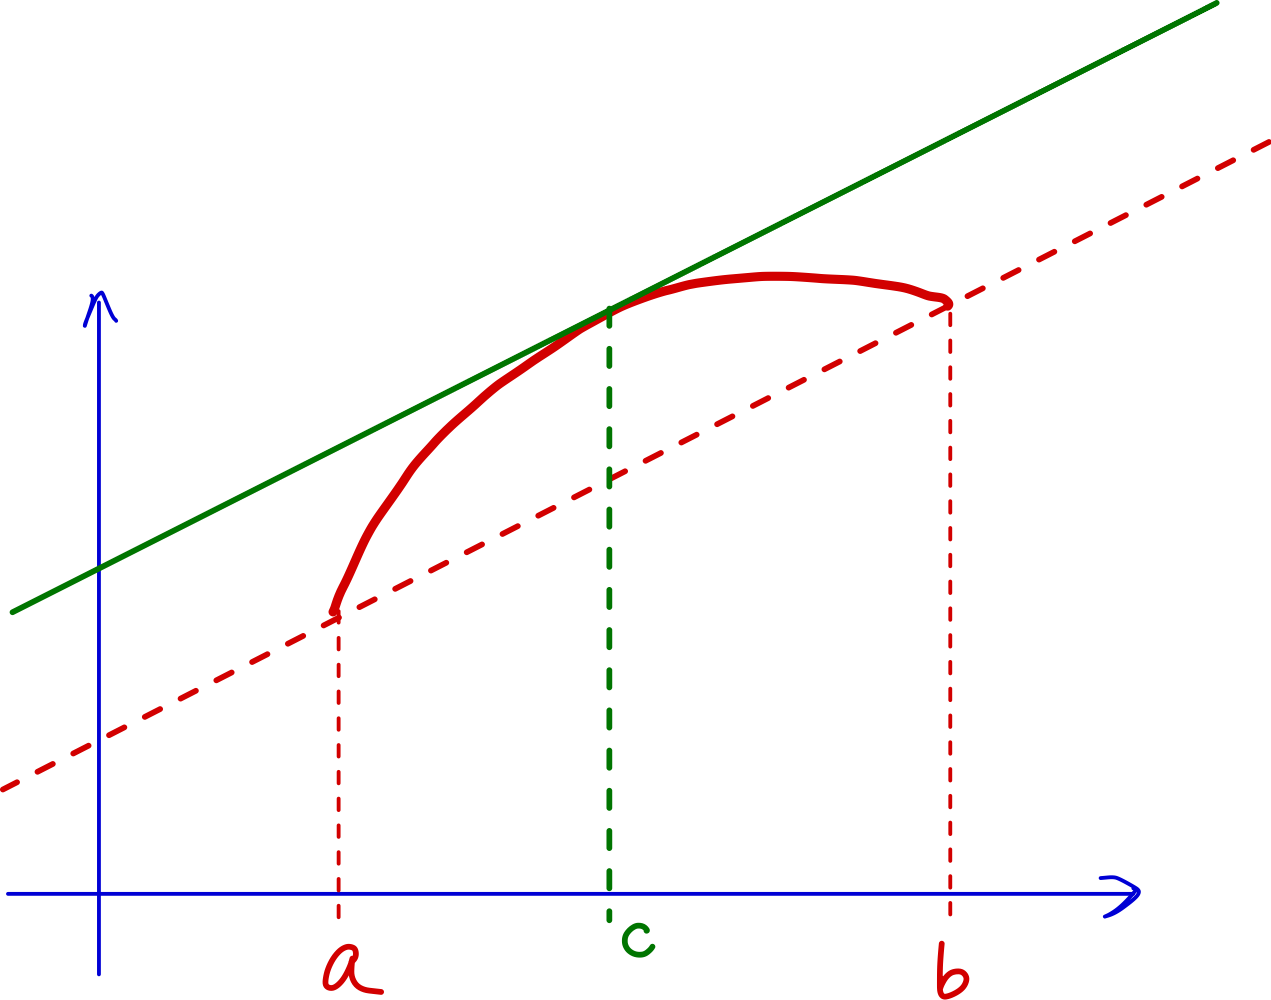
\includegraphics[width=.6\textwidth]{pics/tvm.png}}

\begin{theorem}[Teorema del Valor Medio (de Lagrange)]\label{T:TVM}
       Si $f$ es continua en $[a,b]$ y derivable en $(a,b)$, entonces existe $c\in(a,b)$ tal que 
       \[
       f'(c)=\frac{f(b)-f(a)}{b-a}.
       \]
\end{theorem}

\begin{proof}
    Para demostrar este teorema, consideramos la ecuación de la recta  que pasa por $(a,f(a))$ y $(b,f(b))$:
    \[
    y - f(a) = \frac{f(b)-f(a)}{b-a} (x-a),
    \]
    que puede escribirse también como
    \[    
    y = f(a) + \frac{f(b)-f(a)}{b-a} (x-a).
    \]
    Ahora definimos la función 
    \[
    g(x) = f(x) - \left[ f(a) + \frac{f(b)-f(a)}{b-a} (x-a) \right].
    \]
    Esta función cumple que es continua en $[a,b]$ y derivable en $(a,b)$. Además:
    \begin{align*}
        g(a) &= f(a) - \left[ f(a) + \frac{f(b)-f(a)}{b-a} \underbrace{(a-a)}_0 \right] 
        = f(a)-f(a)=0,
        \\
        g(b) &= f(b) - \left[ f(a) + \frac{f(b)-f(a)}{\cancel{b-a}} \cancel{(b-a)} \right] 
        = f(b)-\left[f(a)+f(b)-f(a)\right] = 0.
    \end{align*}
    Por lo tanto, $g(a)=g(b)=0$ y $g$ cumple las hipótesis del Teorema de Rolle, y luego existe $c\in(a,b)$ tal que $g'(c)=0$. 
    Si calculamos la derivada de $g$, vemos que
    \[
    g'(x) = f'(x) - \frac{f(b)-f(a)}{b-a} \cdot 1,
    \]
    y luego 
    \[
    0 = g'(c) = f'(c) - \frac{f(b)-f(a)}{b-a} ,
    \]
    que inmediatamente implica lo que queríamos demostrar.
\end{proof}

Pasamos ahora a probar consecuencias del Teorema del Valor Medio.

En primer lugar, recordemos que la derivada de una función constante es la función nula.
Nos planteamos la pregunta recíproca. Si una función tiene derivada nula en todo punto: ?`Es esa función necesariamente constante?
La respuesta es efectivamente afirmativa:

\begin{proposition}
    Si $f$ es continua en $[a,b]$, derivable en $(a,b)$ y $f'(x)=0$, para todo $x\in(a,b)$, entonces % existe $k\in\R$ tal que 
    \[ 
    f(x)=f(a), \quad\text{para todo $x\in [a,b]$}.
    \]
\end{proposition}

\begin{proof}
    Sea $x_0 \in (a,b]$. Luego $[a,x_0]\subset [a,b]$ y resulta que $f$ es continua en $[a,x_0]$ y derivable en $(a,x_0)$. Entonces cumple las hipótesis del Teorema del valor medio en el intervalo $[a,x_0]$, por lo tanto, existe $c\in [a,x_0]$ tal que 
    \[
    f'(c) = \frac{f(x_0)-f(a)}{x_0-a}.
    \]
    Pero $f'(c)=0$ por lo que $f(x_0)-f(a)=0$ que a su vez implica $f(x_0)=f(a)$. Con esto concluye nuestra demostración.
\end{proof}

\begin{corollary}\label{C:f=g+k}
    Si $f$ y $g$ son continuas en $[a,b]$, derivables en $(a,b)$ y $f'(x)=g'(x)$, para todo $x\in(a,b)$, entonces existe $C\in\R$ tal que 
    \[ 
    f(x)=g(x)+C, \quad\text{para todo $x\in [a,b]$}.
    \]
\end{corollary}

\begin{proof}
    Definimos $h(x)=f(x)-g(x)$. Luego 
    \[
    h'(x)=f'(x)-g'(x)=0, \quad\text{para todo $x\in [a,b]$}.
    \]
    Entonces $f(x)-g(x)=f(a)-g(a)$, para todo $x\in[a,b]$. 
    Llamando $C=f(a)-g(a)$ se obtiene el resultado deseado.
\end{proof}

El siguiente resultado es una consecuencia importante del Teorema del Valor Medio, que nos permite deducir información de $f$ a partir de información sobre su derivada $f'$.

\begin{proposition}\label{P:signo-derivada=>tendencia}
    Sea $f$ una función continua en $[a,b]$ y derivable en $(a,b)$:
    \begin{enumerate}
        \item Si $f'(x)>0$ para todo $x\in(a,b)$, entonces $f$ es estrictamente creciente en $[a,b]$, 
        es decir, si $a\le x_1<x_2\le b$, entonces $f(x_1)<f(x_2)$.
        \item Si $f'(x)<0$ para todo $x\in(a,b)$, entonces $f$ es estrictamente decreciente en $[a,b]$,
        es decir, si $a\le x_1<x_2\le b$, entonces $f(x_1)>f(x_2)$.
    \end{enumerate}
\end{proposition}

\begin{proof}
    \begin{enumerate}
        \item Sean $x_1,x_2\in[a,b]$ con $x_1<x_2$, es decir, $a\le x_1<x_2\le b$. Consideramos $f$ sobre el intervalo $[x_1,x_2]$ resulta que $f$ es continua en ese intervalo y derivable en $(x_1,x_2)$. Es decir, satisface las hipótesis del Teorema del Valor Medio (Teorema~\ref{T:TVM}) en el intervalo $[x_1,x_2]$.
        Por lo tanto, existe $c\in(x_1,x_2)$ tal que 
        \[
        \frac{f(x_2)-f(x_1)}{x_2-x_1} = f'(c).
        \]
        O sea,
        \[
        f(x_2)-f(x_1) = f'(c)\, (x_2-x_1).
        \]
        Pero $f'(c)>0$, por lo que $f(x_2)-f(x_1)>0$, o lo que es lo mismo, $f(x_2)>f(x_1)$.
        
        \item Se prueba de la misma manera, sólo que ahora $f'(c)<0$ y por lo tanto $f(x_2)-f(x_1)<0$, que es lo mismo que decir $f(x_2)<f(x_1)$.\qedhere
    \end{enumerate}
\end{proof}

Presentamos ahora un teorema importante que nos va a servir para calcular las derivadas de más funciones.

\begin{theorem}[Derivada de la función inversa]
    Sea $f$ una función continua y estrictamente creciente, o estrictamente decreciente en $[a,b]$ (con lo cual existe inversa):
    \begin{itemize}
        \item $\D f^{-1}:[f(a),f(b)]\to [a,b]$ cuando $f$ es estrictamente creciente;
        \item $\D f^{-1}:[f(b),f(a)]\to [a,b]$ cuando $f$ es estrictamente decreciente.
    \end{itemize}
    Si $x\in(a,b)$ es un punto tal que $f$ es derivable en $x$, y $f'(x)\neq 0$, entonces $f^{-1}$ es derivable en $y=f(x)$ y además:
    \[
    \big(f^{-1}\big)'(y) = \frac1{f'(x)},
    \]
    que también podemos escribir así:
    \begin{equation}\label{eq:derivada inversa}
    \big(f^{-1}\big)'(f(x)) = \frac1{f'(x)},
    \qquad\text{o}\qquad
    \big(f^{-1}\big)'(y) = \frac1{f'(f^{-1}(y))},
    \end{equation}
\end{theorem}

\begin{proof}
    La demostración se verá en la clase de \emph{Coloquio de Demostraciones}.
\end{proof}

Si bien esta demostración es un poco complicada, la parte complicada es demostrar que $f\inv$ es derivable. Suponiendo que es derivable, la fórmula es sencilla a partir de la regla de la cadena. En efecto, por definición de función inversa, $f\circ f\inv(y) = y$, luego, por un lado
\[
\frac{d (f\circ f\inv)(y)}{dy} = \frac{dy}{dy} = 1,
\]
y por otro lado, usando la regla de la cadena,
\[
    \frac{d (f\circ f\inv)(y)}{dy} = f'\big(f\inv(y)\big)\cdot (f\inv)'(y).
\]
Luego,
\[
    f'\big(f\inv(y)\big)\cdot (f\inv)'(y)=1
    \quad\implies\quad  (f\inv)'(y)= \frac1{f'\big(f\inv(y)\big)}.
\]

\begin{example}
    Consideremos la función $f:\R\to\R$ dada por $f(x)=\sen x$. 
    Su derivada es $f'(x)=\cos x$, que es positiva en el intervalo $-\frac\pi2<x<\frac\pi2$.
    Luego, el seno es una función estrictamente creciente en $[-\pi/2,\pi/2]$ y como además es continua, existe función inversa 
    \[
    \arcsen: [-1,1] \to \Big[-\frac\pi2,\frac\pi2\Big]:
    \qquad
    \arcsen y = x \quad\iff\quad \sen x = y.
    \]

    \centerline{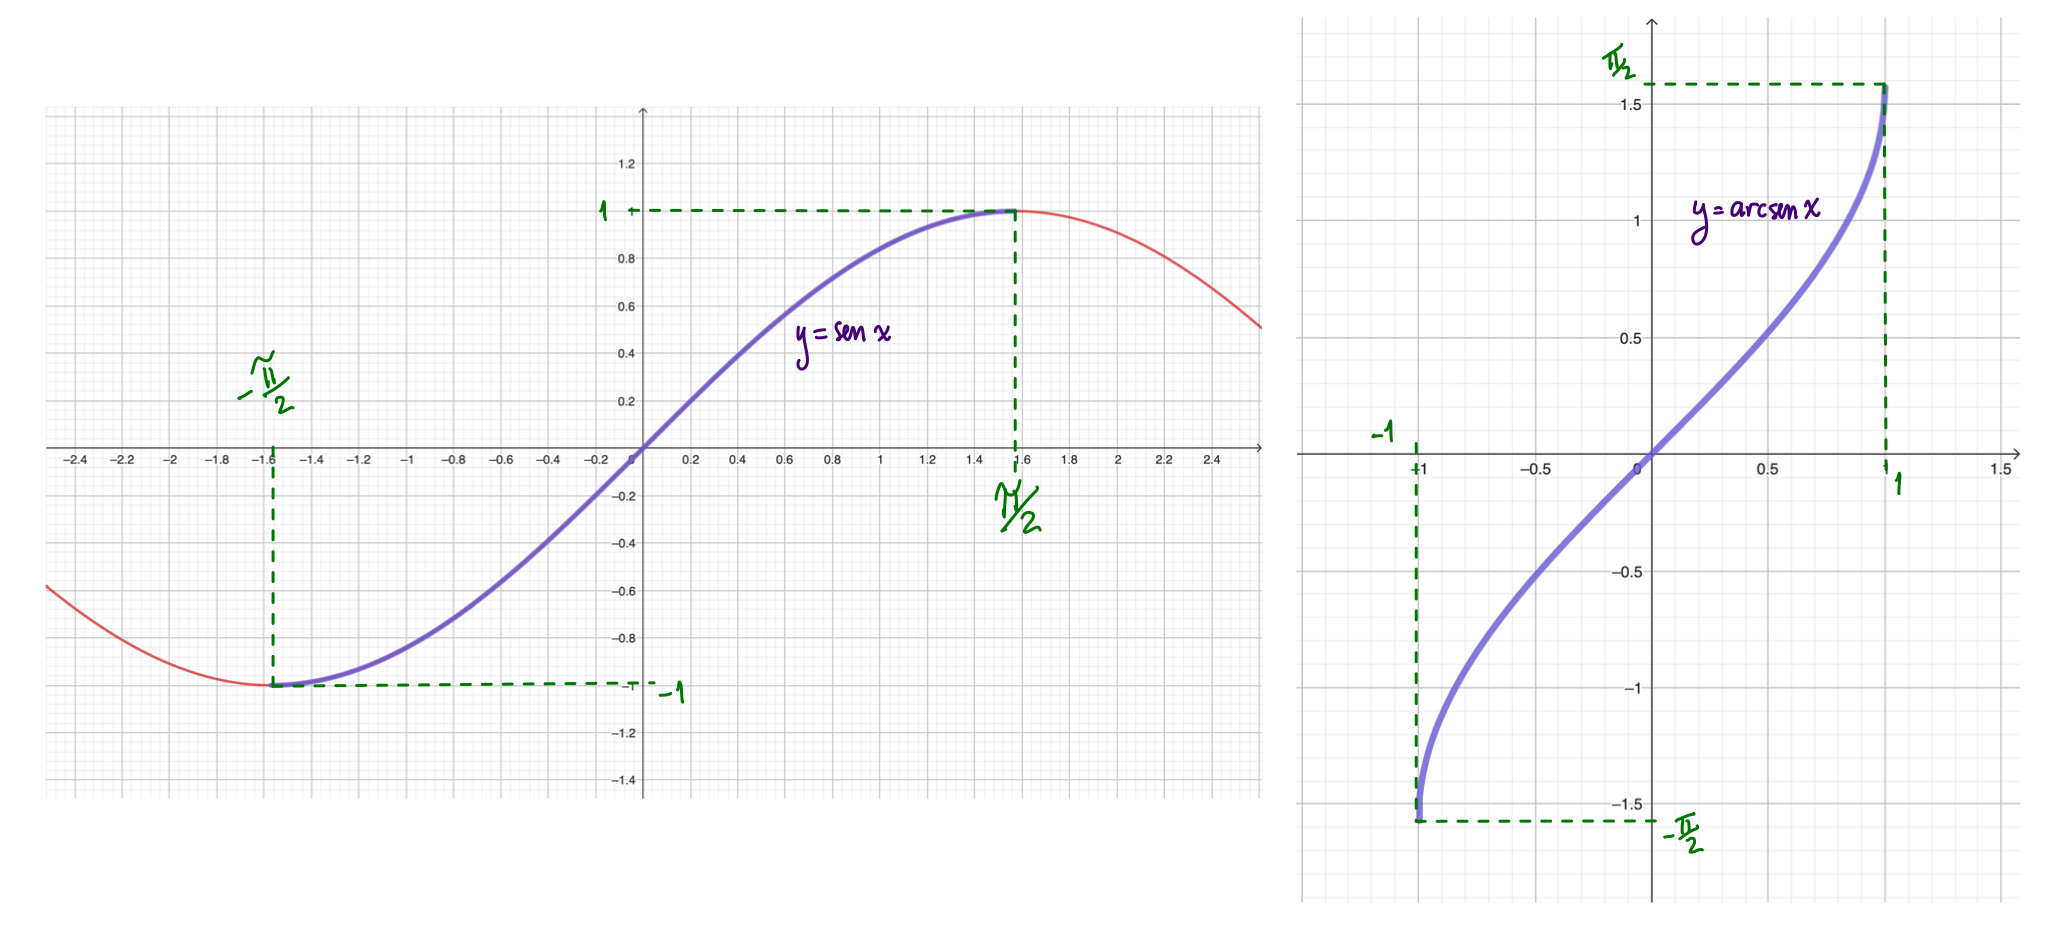
\includegraphics[width=.8\textwidth]{pics/seno-arcseno.jpeg}}
    
    Como $\sen'(x)=\cos(x)\neq 0$ en $\big(-\frac\pi2,\frac\pi2\big)$, entonces $\arcsen$ es derivable en $(-1,1)$.
    Para hallar su derivada, usamos la segunda fórmula de~\eqref{eq:derivada inversa}:
    \[
    \arcsen'(y) = \frac{1}{\sen'(\arcsen y)}
    = \frac1{\cos(\arcsen y)} = \frac1{\cos x},
    \]
    donde $x=\arcsen y$. Entonces $\sen x=y$, y tenemos que deducir cuánto vale $\cos x$ sabiendo que $\sen x = y$. Para esto, utilizaremos que
    \[
    \cos^2 x + \sen^2 x = 1,\qquad\text{y}\qquad x\in\big(-\frac\pi2,\frac\pi2\big).
    \]
    De la primera deducimos que $\cos x = \pm \sqrt{1-y^2}$, como $x\in\big(-\frac\pi2,\frac\pi2\big)$ deducimos que $\cos x > 0$ por lo que $\cos x = \sqrt{1-y^2}$. Luego
    \[
    \arcsen'(y) = \frac1{\sqrt{1-y^2}}, \qquad \text{para $y\in (-1,1)$}.
    \]
\end{example}

\begin{example}
    Consideremos ahora la función $f:\R\to\R$ dada por $f(x)=\cos x$. 
    Su derivada es $f'(x)=-\sen x$, que es negativa en el intervalo $0<x<\pi$.
    Luego, el coseno es una función estrictamente decreciente en $[0,\pi]$ y como además es continua, existe función inversa 
    \[
    \arccos: [-1,1] \to [0,\pi]:
    \qquad
    \arccos y = x \quad\iff\quad \cos x = y.
    \]

    \centerline{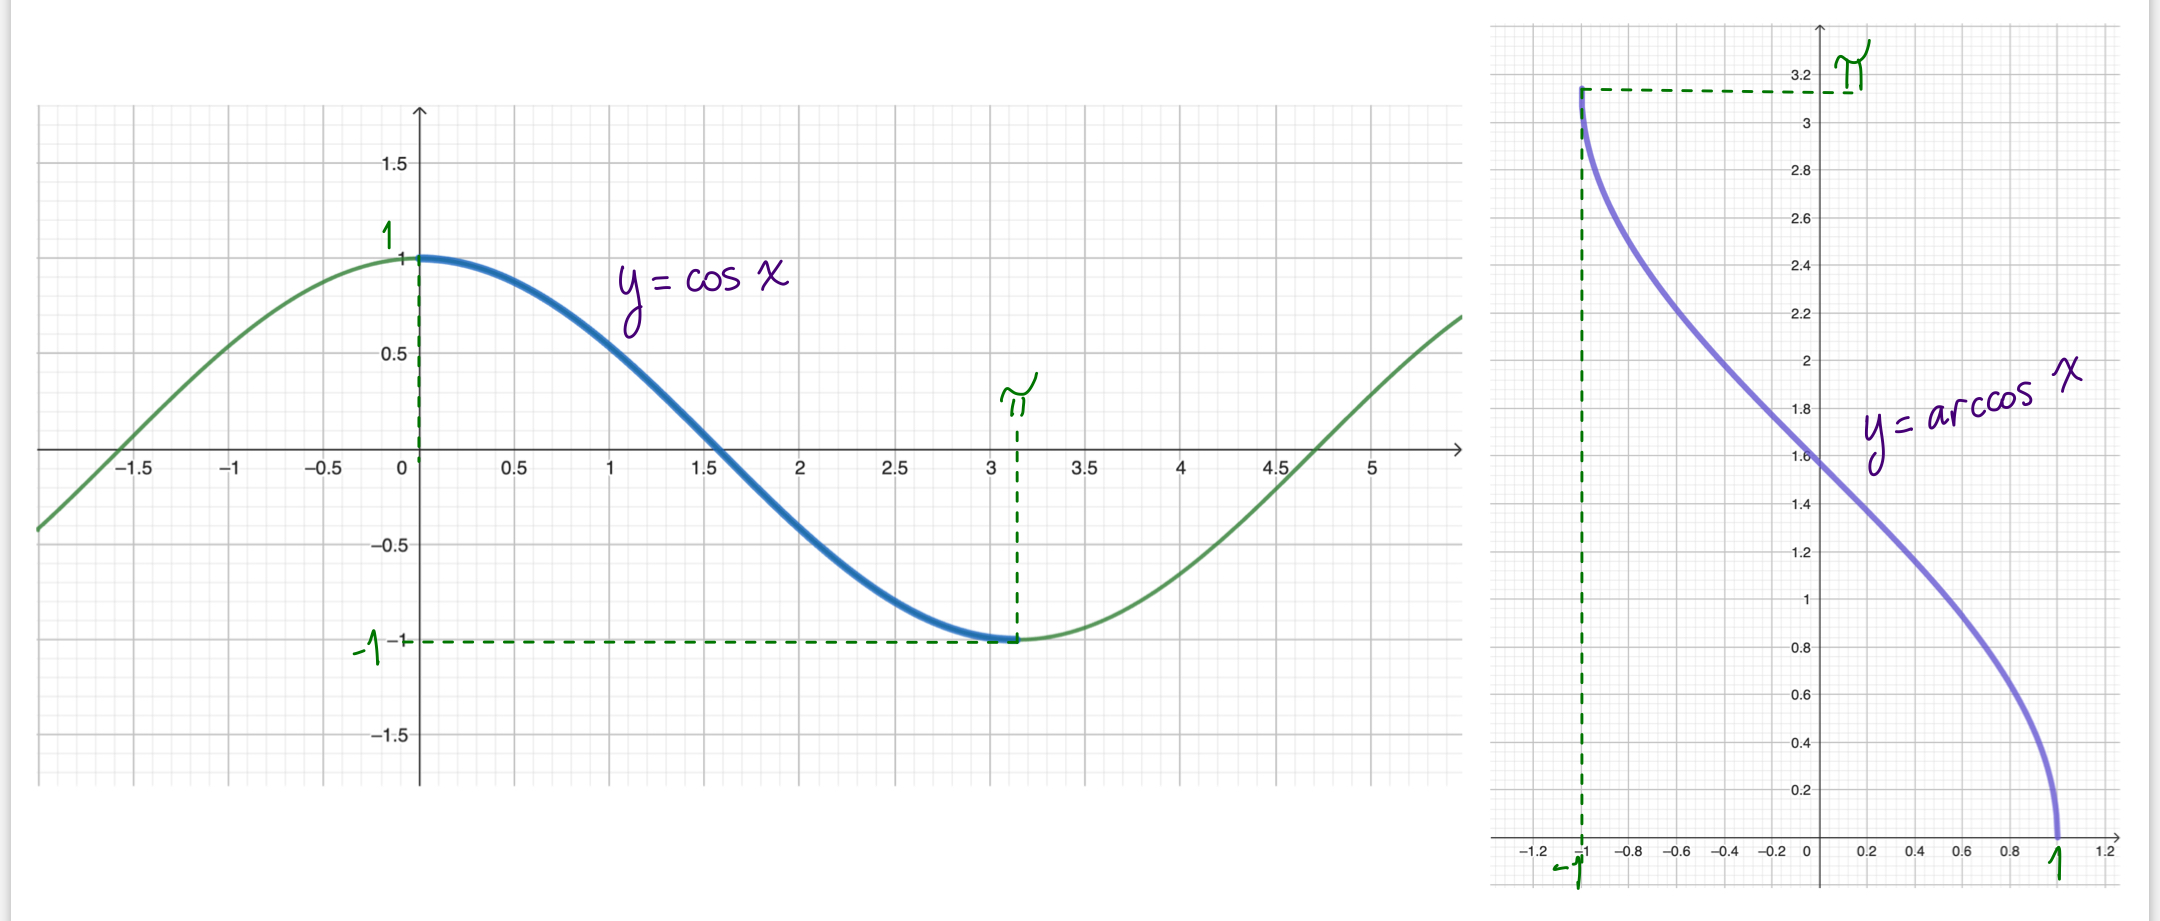
\includegraphics[width=.8\textwidth]{pics/cos-arccos.jpeg}}
    
    Como $\cos'(x)=-\sen(x)\neq 0$ en $(0,\pi)$, entonces $\arccos$ es derivable en $(-1,1)$.
    Para hallar su derivada, usamos la segunda fórmula de~\eqref{eq:derivada inversa}:
    \[
    \arccos'(y) = \frac{1}{\cos'(\arccos y)}
    = -\frac1{\sen(\arccos y)} = -\frac1{\sen x},
    \]
    donde $x=\arccos y$. Entonces $\cos x=y$, y tenemos que deducir cuánto vale $\sen x$ sabiendo que $\cos x = y$. Para esto, utilizaremos que
    \[
    \cos^2 x + \sen^2 x = 1,\qquad\text{y}\qquad x\in(0,\pi).
    \]
    De la primera deducimos que $\sen x = \pm \sqrt{1-y^2}$, como $x\in(0,\pi)$ deducimos que $\sen x > 0$ por lo que $\sen x =  \sqrt{1-y^2}$. Luego
    \[
    \arccos'(y) = -\frac1{\sqrt{1-y^2}}, \qquad \text{para $y\in (-1,1)$}.
    \]
\end{example}

Veamos un último ejemplo:

\begin{example}
    Consideremos ahora la función dada por $\D f(x)=\tan x=\frac{\sen x}{\cos x}$, cuyo dominio es todo $\R$ excepto los puntos de la forma $\frac\pi2+n\pi$, $n\in\Z$, que son los puntos donde se anula el denominador $\cos x$.
    Quedó como ejercicio en una de las secciones anteriores calcular $\tan'(x)$, y la respuesta era
    \[
    \tan'(x)=\frac1{\cos^2x}.
    \]
    Esta derivada es siempre positiva, por lo tanto, $f(x)$ es estrictamente creciente en cada intervalo de la forma $(n\pi-\frac\pi2,n\pi+\frac\pi2)$. Consideremos esta función en el intervalo $(-\frac\pi2,\frac\pi2)$, donde es estrictamente creciente. Observamos que
    \[
    \lim_{x\to-\frac\pi2^+}\tan(x)=-\infty,
    \qquad\text{y}\qquad
    \lim_{x\to\frac\pi2^-}\tan(x)=+\infty.
    \]
    Por lo tanto, la función tangente es biyectiva de $(-\frac\pi2,\frac\pi2)$ en $(-\infty,+\infty)$, y existe función inversa 
    \[
    \arctan: \R \to \Big(-\frac\pi2,\frac\pi2\Big)
    \qquad
    \arctan y = x \quad\iff\quad \tan x = y.
    \]

    \centerline{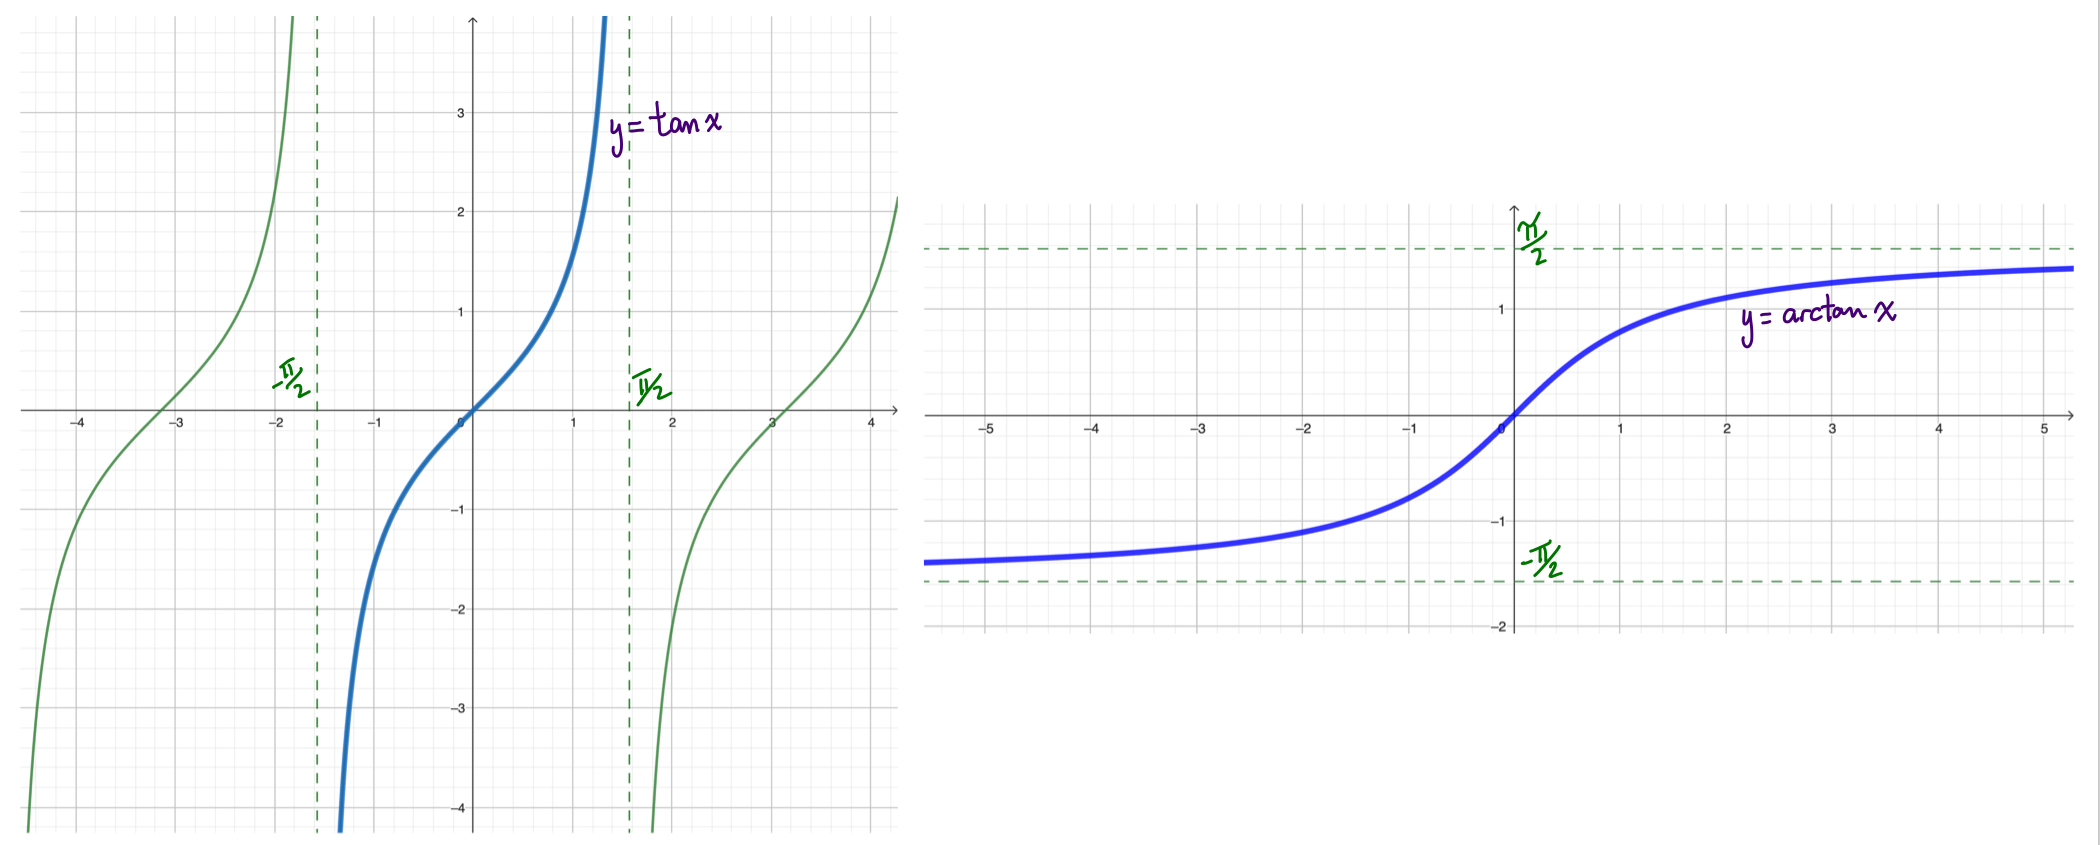
\includegraphics[width=.8\textwidth]{pics/tan-atan.jpeg}}
    
 Como $\tan'(x)=\frac1{\cos^2(x)}> 0$ en $(-\frac\pi2,\frac\pi2)$, entonces $\arctan$ es derivable en $\R$.
    Para hallar su derivada, usamos la segunda fórmula de~\eqref{eq:derivada inversa}:
    \[
    \arctan'(y) = \frac{1}{\tan'(\arctan y)}
    = \frac1{\frac1{\cos^2(\arctan y)}} 
    = \cos^2(\arctan y)
    = \cos^2 x,
    \]
    donde $x=\arctan y$. Entonces $\tan x=y$, y tenemos que deducir cuánto vale $\cos^2 x$ sabiendo que $\tan x = y$. 
    Veamos
    \begin{align*}
        \frac{\sen x}{\cos x} = y
        &\implies
        \frac{\sen^2 x}{\cos^2 x} = y^2
        \implies 
        \frac{1-\cos^2 x}{\cos^2 x} = y^2
        \\
        &\implies
        1-\cos^2 x = y^2 \, \cos^2x
        \implies 
        1 = \cos^2 x + y^2 \, \cos^2x
        = \cos^2 x \, \big(1+y^2\big)
        \\
        &\implies \cos^2x = \frac1{1+y^2}.
    \end{align*}
    De aquí obtenemos que
    \[
    \arctan'(y) =  \frac1{1+y^2},
    \quad\text{para todo $y\in\R$.}
    \]
\end{example}


\subsubsection*{Ejercicios de la sección~\getcurrentref{chapter}.\getcurrentref{section}}

\begin{enumerate}
\item * Si $f:\R\to\R$ es continua en $\R$ y derivable en todo punto de $\R\setminus\{a\}$, y existe $\D\lim_{x\to a}f'(x)= \ell$, entonces $f$ es derivable en $x=a$ y $f'(a) = \ell$.
Usar el Teorema del Valor Medio (de Lagrange) para calcular las derivadas laterales.

\item Probar las siguientes afirmaciones para una función $f:[a,b]\to \R$ continua en $[a,b]$ y derivable en $(a,b)$:
\begin{enumerate}
  \item Si $f'(x)\ge 0$ para todo $x\in(a,b)$, entonces $f$ es creciente en $[a,b]$; es decir, $a\le x_1<x_2\le b$ implica $f(x_1)\le f(x_2)$.
  \item Si $f$ es creciente, entonces $f'(x)\ge 0$ para todo $x\in(a,b)$.
  \item Si $f'(x)\le 0$ para todo $x\in(a,b)$, entonces $f$ es decreciente en $[a,b]$; es decir, $a\le x_1<x_2\le b$ implica $f(x_1)\ge f(x_2)$
  \item Si $f$ es decreciente, entonces $f'(x)\le 0$ para todo $x\in(a,b)$.
\end{enumerate}

\item Encontrar un ejemplo de una función $f:\R\to\R$ que sea estrictamente creciente y derivable, pero que no cumpla que $f'(x)>0$, para todo $x\in\R$.

\item Probar que la función $f(x)=\sqrt[3]{(x-3)^2}$ satisface $f(1)=f(5)$ pero no existe $c\in(1,5)$ tal que $f'(c)=0$. ?`Por qué no se puede aplicar el Teorema de Rolle?

\item Sea $f(x)=(x-1)\, x\, (x+2)\, (x+5)$. Probar que $f'(x)$ tiene tres raíces reales.

\item Para cada una de las siguientes funciones, determinar el punto $c\in(0,1)$ que cumple el Teorema del Valor Medio en el intervalo $[0,1]$:
\begin{multicols}{3}
  \begin{enumerate}
    \item $f(x)=3x$;
    \item $f(x)=2x^2$;
    \item $f(x)=\sqrt[3]{x}$.
  \end{enumerate}
\end{multicols}

\item Hallar $f'(x)$ para:
\begin{multicols}{2}

  \begin{enumerate}
    \item $\D f(x) = \arcsen(\sqrt x)$;
    \item $\D f(x) = \arccos(x^2+1)$;
    \item $\D f(x) = \big(e^{\arcsen (1/x)}\big)^x$;
    \item $\D f(x) = \sqrt[3]{\arccos\Big(\frac{x^2}{1+x^2}\Big)}$;
    \item $\D f(x) = \ln\big(\arccos (x)\big)$;
  \end{enumerate}
  
\end{multicols}
\end{enumerate}

\section{Máximos y mínimos locales}

\begin{definition}
    Consideremos una función $f:I\to \R$, donde $I$ es un intervalo.
    Decimos que $f$ tiene un \emph{máximo local en $x_0$} cuando existe $\delta>0$ tal que
    \[
    f(x_0)\ge f(x), \quad\text{para todo $x$ en $(x_0-\delta,x_0+\delta)\cap I$}.
    \]
    Decimos que $f$ tiene un \emph{mínimo local en $x_0$} cuando existe $\delta>0$ tal que
    \[
    f(x_0)\le f(x), \quad\text{para todo $x$ en $(x_0-\delta,x_0+\delta)\cap I$}.
    \]
\end{definition}

\begin{figure*}[htbp]
    \centerline{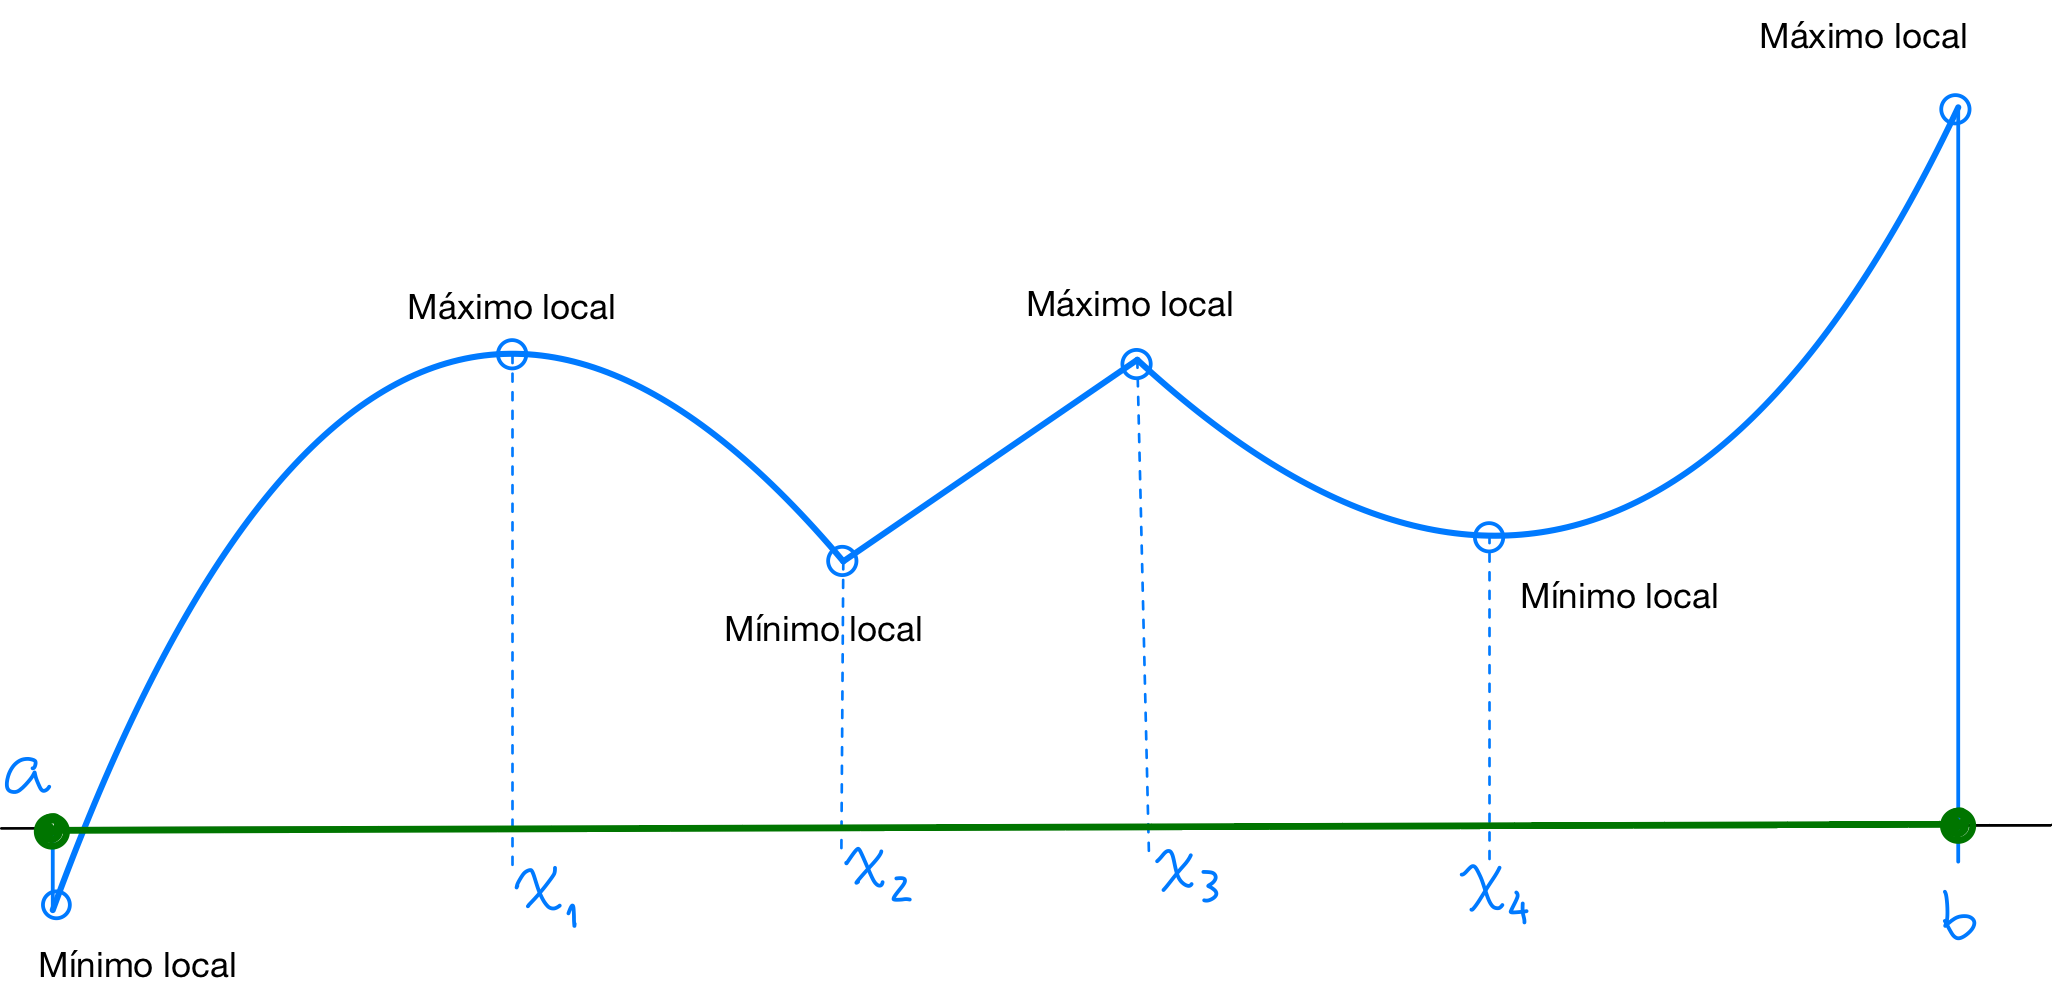
\includegraphics[width=.8\textwidth]{pics/max-min-locales-int-cerrado.png}}
\caption{Máximos y mínimos locales en un intervalo cerrado.}
\end{figure*}

Observamos lo siguiente, con respecto a los máximos y mínimos de una función $f$ en un intervalo cerrado $[a,b]$:
\begin{itemize}
    \item Si $f$ es creciente en un intervalo $[a,a+\delta]$, para algún $\delta>0$, entonces $f(a)$ es un mínimo local de $f$.
    \item Si $f$ es decreciente en un intervalo $[a,a+\delta]$, para algún $\delta>0$, entonces $f(a)$ es un máximo local de $f$.
    \item Si $f$ es creciente en un intervalo $[b-\delta,b]$, para algún $\delta>0$, entonces $f(b)$ es un máximo local de $f$.
    \item Si $f$ es decreciente en un intervalo $[b-\delta,b]$, para algún $\delta>0$, entonces $f(b)$ es un mínimo local de $f$.
    \item Si $x_0\in(a,b)$ y $f$ es decreciente en $[x_0-\delta,x_0]$ y creciente en $[x_0,x_0+\delta]$, para algún $\delta>0$, entonces $f$ tiene un mínimo local en $x_0$.
    \item Si $x_0\in(a,b)$ y $f$ es creciente en $[x_0-\delta,x_0]$ y decreciente en $[x_0,x_0+\delta]$, para algún $\delta>0$, entonces $f$ tiene un máximo local en $x_0$.
\end{itemize}

\begin{figure*}[htbp]
    \centerline{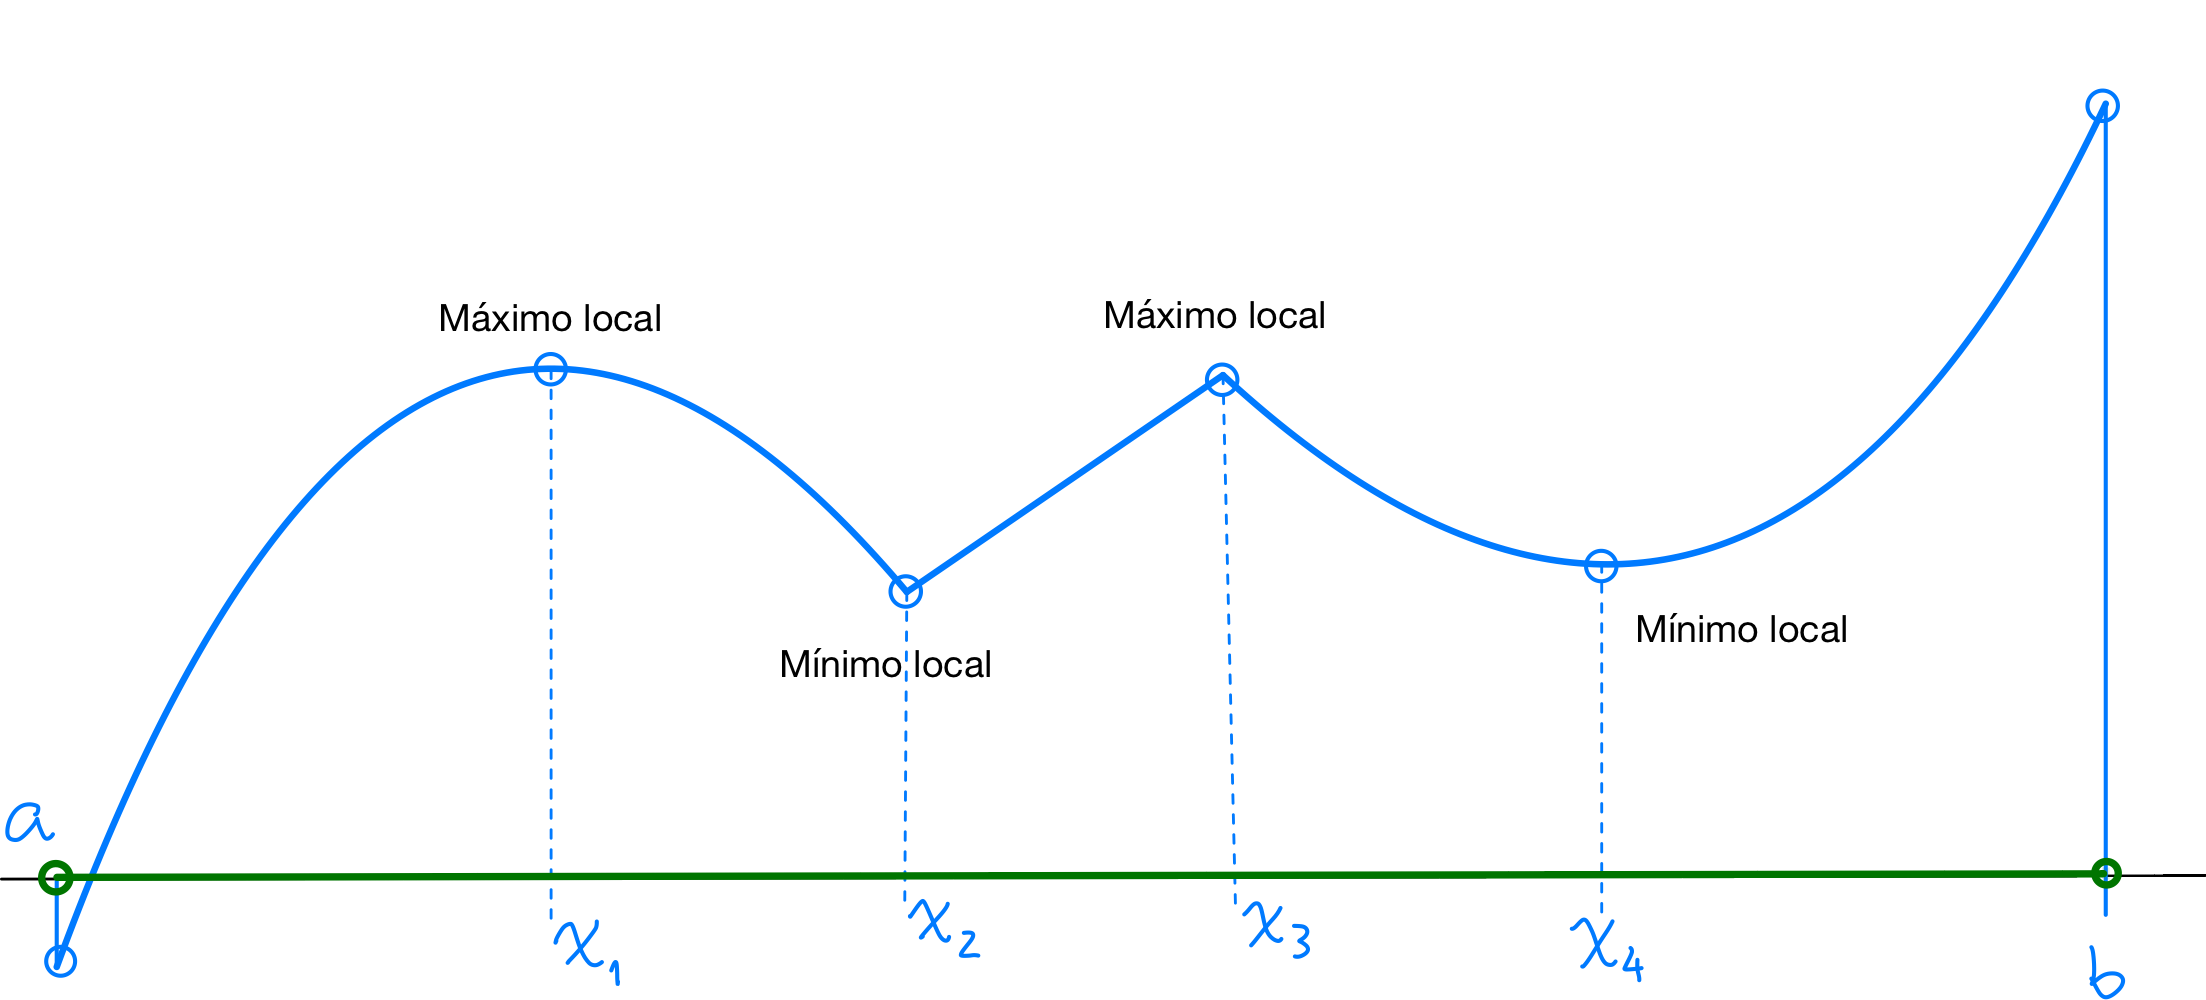
\includegraphics[width=.8\textwidth]{pics/max-min-locales-int-abierto.png}}
\caption{Máximos y mínimos locales en un intervalo abierto.}
\end{figure*}


A continuación vemos un teorema que nos permite determinar los puntos \emph{candidatos} a puntos máximos o mínimos.

\begin{theorem}
    Sea $f:I\to\R$. Si $f$ tiene un máximo o un mínimo local en $x_0$, entonces ocurre una de las tres siguientes:
    \begin{itemize}
        \item $x_0$ es un extremo del intervalo;
        \item $f'(x_0)$ no existe;
        \item $f'(x_0)=0$.
    \end{itemize}
\end{theorem}

\begin{proof}
    Supongamos que $f$ tiene un máximo local en $x_0$ que no es un extremo del intervalo y que $f'(x_0)$ existe; si $x_0$ es un extremo del intervalo o $f'(x_0)$ no existe, no hay nada que probar.

    Luego, existe $\delta > 0$ tal que $f(x)\ge f(x_0)$, para todo $x\in(x_0-\delta,x_0+\delta)$.

    Si existe $f'(x_0)$, entonces
    \[
    f'(x_0)= \limxop \frac{f(x)-f(x_0)}{x-x_0} = \limxom \frac{f(x)-f(x_0)}{x-x_0}.
    \]
    Ahora bien, si $x_0<x<x_0+\delta$, entonces $f(x)\ge f(x_0)$ y por lo tanto $\frac{f(x)-f(x_0)}{x-x_0}\ge 0$. Luego
    \[
    f'(x_0) = \limxop \frac{f(x)-f(x_0)}{x-x_0} \ge 0.
    \]
    Además, si $x_0-\delta <x<x_0$, entonces $f(x)\ge f(x_0)$ y por lo tanto $\frac{f(x)-f(x_0)}{x-x_0}\le 0$. Luego
    \[
    f'(x_0) = \limxom \frac{f(x)-f(x_0)}{x-x_0} \le 0.
    \]
    Esto implica que $f'(x_0)=0$.

    El caso en que $f$ tiene un mínimo local es similar.
\end{proof}

Los puntos \emph{candidatos} a ser puntos máximos o mínimos de una función reciben el nombre de \emph{puntos críticos}.
\begin{definition}[Puntos críticos]
    Dada una función $f:I\to \R$, llamamos puntos críticos a los siguientes puntos:
    \begin{itemize}
        \item Extremos del intervalo que pertenezcan al intervalo;
        \item Puntos $x_0$ del interior de $I$ donde la derivada no existe;
        \item Puntos $x_0$ donde $f'(x_0)=0$.
    \end{itemize}
\end{definition}

En vista del teorema y de la definición anteriores, cuando buscamos máximos y mínimos locales, los únicos números que necesitamos considerar son los puntos críticos de $f$.
Ilustramos ahora con ejemplos la técnica para hallar los máximos y mínimos locales con algunos ejemplos. En cada ejemplo, el primer paso consiste en hallar los puntos críticos.

\begin{example}
    Consideremos la función $f(x)=3-x^2$ en $\R$. 
    El intervalo considerado es $(-\infty,+\infty)$ que no tiene extremos.
    Esta función es polinomial y por lo tanto derivable, con 
    \[f'(x)=-2x.\]
    Ahora planteamos la ecuación $f'(x)=0$, es decir $-2x=0$, que tiene como única solución $x=0$.

    Es decir, $x=0$ es el único punto crítico. El número $f(0)=3$ es un máximo local porque $f(x)=3-x^2\le 3$, para todo $x\in\R$.
\end{example}

\begin{example}
    Consideremos ahora la siguiente función en $[0,+\infty)$
    \[ 
    f(x)=|x-3|+2=\begin{cases}
        -x+5,\quad&\text{si $x<3$},
        \\
        x-1,\quad&\text{si $x\ge 3$}.
    \end{cases}
    \]
    cuya derivada es 
    \[ 
    f'(x)=\begin{cases}
        -1,\quad&\text{si $x<3$},
        \\
        \text{no existe},\quad&\text{si $x=3$},
        \\
        1,\quad&\text{si $x> 3$}.
    \end{cases}
    \]
    El intervalo que estamos considerando tiene un solo extremo, $x=0$, y la derivada de $f$ no se anula nunca. Por lo tanto, los puntos críticos son:
    \begin{itemize}
        \item $x=0$, extremo izquierdo del intervalo;
        \item $x=3$, $f'(3)$ no existe.
    \end{itemize}
    Si observamos cerca de $x=0$, la función es $f(x)=-x+5$, para $0\le x<3$, por lo tanto
    \[f(0)= 5 \ge -x+5, \quad\text{para todo $0\le x < 3$}.\]
    Entonces $f$ tiene un máximo local en $x=0$.

    En el otro punto crítico, $x=3$, vemos, que:
    \[
    f(3)=2\le f(x)=|x-3|+2=\begin{cases}
        -x+5,\quad&\text{si $0<x\le 3$},
        \\
        x-1,\quad&\text{si $x\ge 3$}.
    \end{cases}
    \]
    Por lo tanto, $f$ tiene un mínimo local en $x=3$.
\end{example}

\begin{example}
    Consideremos ahora $f(x)=x^3$, en el intervalo $[-1,1]$. Esta función es derivable con $f'(x)=3\, x^2$. Los puntos críticos son:
    \begin{itemize}
        \item $x=-1$, extremo izquierdo;
        \item $x=1$, extremo derecho;
        \item $x=0$, donde $f'$ se anula.
    \end{itemize}
    Si analizamos el valor de la función en estos tres puntos, vemos que
    
    \begin{center}
        \begin{tabular}{|c|c|}
            \hline
            $x$ & $f(x)$ \\
            \hline 
            $-1$ & $-1$ \\
            $0$ & $0$ \\
            $1$ & $1$ \\
            \hline
        \end{tabular}
    \end{center}
    En $x=-1$ hay un mínimo local y en $x=1$ hay un máximo local, dado que $f'(x)=3 x^2\ge 0$ en $(-1,1)$ y por lo tanto $f$ es creciente. ?`Qué ocurre en $x=0$? Este punto es un punto crítico, donde no hay ni un máximo ni un mínimo, ya que:
    \[
    \begin{cases}
        f(x) \ge f(0)=0,\quad&\text{si $x\ge 0$},
        \\
        f(x) \le f(0)=0,\quad&\text{si $x\le 0$}.
    \end{cases}\]
\end{example}

Concluimos en base al último ejemplo que los puntos críticos son los \emph{candidatos} a ser puntos máximos o mínimos, pero no son todos puntos máximos o mínimos. Una herramienta para determinar si un punto crítico corresponde a un máximo o mínimo local la da la siguiente proposición.

\begin{proposition}[Criterio de la derivada primera]
    Supongamos que $x_0$ es un punto crítico de $f$ donde $f$ es continua, en el interior del intervalo que estamos considerando. Supongamos que existe $\delta>0$ tal que:
    \begin{enumerate}
        \item $f'(x)>0$ para todo $x\in(x_0-\delta,x_0)$ y $f'(x)<0$, para todo $x\in(x_0,x_0+\delta)$, entonces $f(x_0)$ es un máximo local; 
        \item $f'(x)<0$ para todo $x\in(x_0-\delta,x_0)$ y $f'(x)>0$, para todo $x\in(x_0,x_0+\delta)$, entonces $f(x_0)$ es un mínimo local; 
        \item $f'(x)$ tiene el mismo signo en $(x_0-\delta,x_0)$ y en $(x_0,x_0+\delta)$, entonces $f(x_0)$ no es ni un máximo ni un mínimo local.
    \end{enumerate}
\end{proposition}

Esta proposición puede decirse, en palabras, de la siguiente manera:
\begin{quote}
    \begin{enumerate}
        \item $f'>0$ a la izquierda de $x_0$ y $f'<0$ a la derecha de $x_0$, entonces $f(x_0)$ es un máximo local; 
        \item $f'<0$ a la izquierda de $x_0$ y $f'>0$ a la derecha de $x_0$, entonces $f(x_0)$ es un mínimo local; 
        \item $f'$ no cambia de signo en $x_0$, entonces $f(x_0)$ no es ni un máximo ni un mínimo local.
    \end{enumerate}
\end{quote}

\centerline{
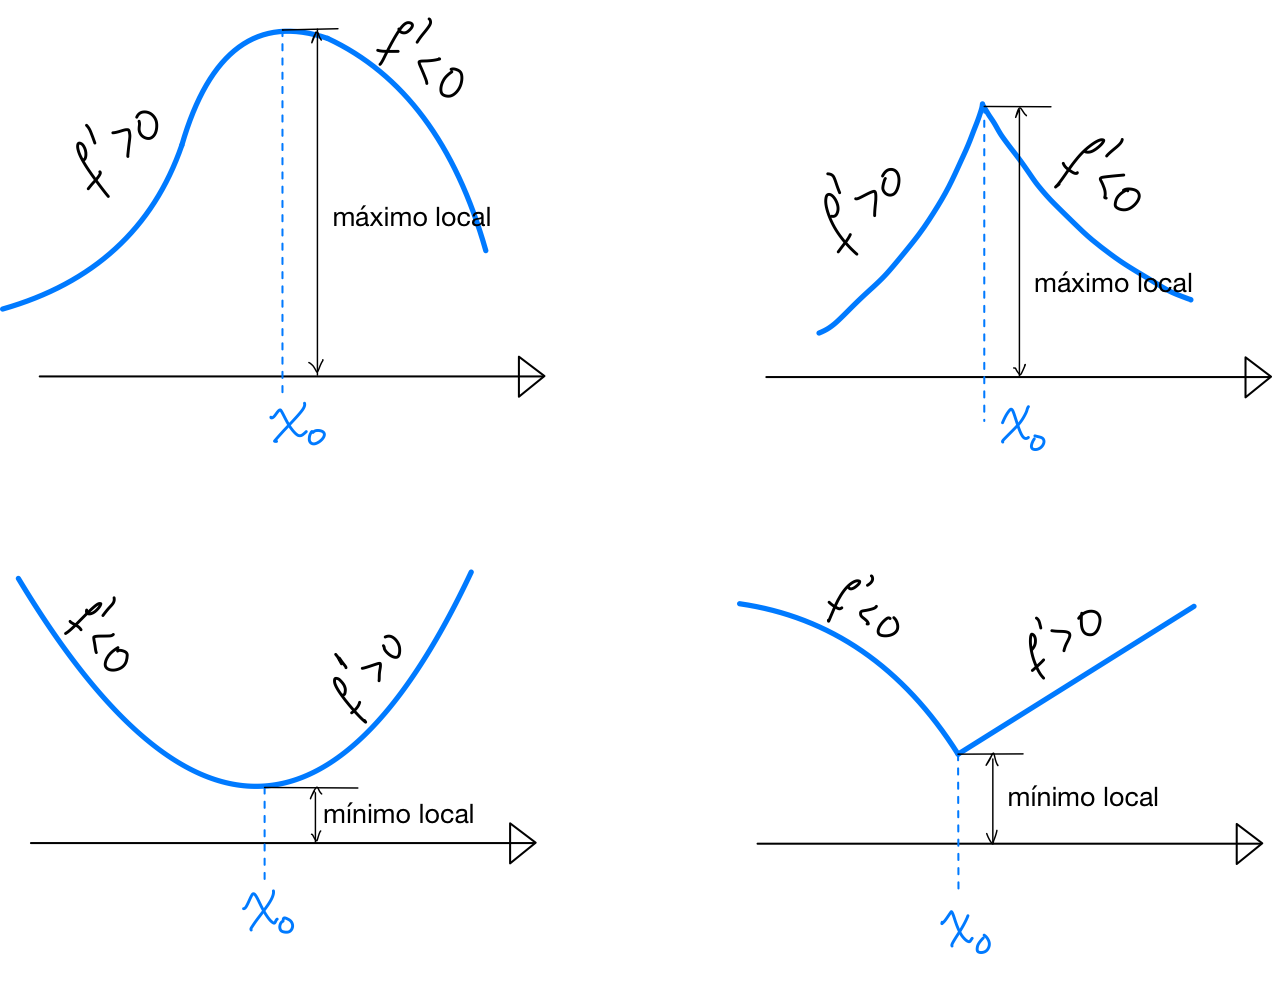
\includegraphics[width=.8\textwidth]{pics/max-min-locales-derivada.png}
}
La demostración es sencilla, haciendo uso de la Proposición~\ref{P:signo-derivada=>tendencia}.
\begin{proof}
    \begin{enumerate}
        \item Por la Proposición~\ref{P:signo-derivada=>tendencia}, $f$ es creciente en $[x_0-\delta,x_0]$ y decreciente en $[x_0,x_0+\delta]$, por lo tanto $f(x_0)\ge f(x)$, para todo $x\in[x_0-\delta,x_0+\delta]$.
        \item Por la Proposición~\ref{P:signo-derivada=>tendencia}, $f$ es decreciente en $[x_0-\delta,x_0]$ y creciente en $[x_0,x_0+\delta]$, por lo tanto $f(x_0)\le f(x)$, para todo $x\in[x_0-\delta,x_0+\delta]$.
        \item Hay aquí dos casos:
        \begin{enumerate}
            \item $f'(x)<0$ en $(x_0-\delta,x_0)$ y en $(x_0,x_0+\delta)$. En este caso, por la Proposición~\ref{P:signo-derivada=>tendencia}, $f$ es estrictamente decreciente en $[x_0-\delta,x_0+\delta]$.
            Por lo tanto, $f(x_0)<f(x)$, para todo $x\in (x_0-\delta,x_0)$; y
            $f(x_0)>f(x)$, para todo $x\in (x_0,x_0+\delta)$.
            \item $f'(x)>0$ en $(x_0-\delta,x_0)$ y en $(x_0,x_0+\delta)$. En este caso, por la Proposición~\ref{P:signo-derivada=>tendencia}, $f$ es estrictamente creciente en $[x_0-\delta,x_0+\delta]$.
            Por lo tanto, $f(x_0)>f(x)$, para todo $x\in (x_0-\delta,x_0)$; y
            $f(x_0)<f(x)$, para todo $x\in (x_0,x_0+\delta)$.
        \end{enumerate}
        En ambos casos, $f(x_0)$ no es ni un máximo ni un mínimo local de $f$.\qedhere
    \end{enumerate}
\end{proof}

\begin{example}
    Consideremos la función $f(x) = 2x^3-x^4$ en $\R$. Su derivada es
    $$ f'(x) = 6\,x^2-4\,x^3 = 2\, x^2\, (3-2x).$$
    La derivada se anula en $x=0$ y en $x=3/2$. Resumimos el signo de $f'$ en la siguiente tabla:

    \begin{center}
\def\arraystretch{1.5}
\begin{tabular}{|c|c|c|}
            \hline
            $x \in(-\infty,0)$ & $x\in(0, 3/2)$ & $x\in(3/2,+\infty)$ \\
            \hline
            $f'>0$& 
            $f'>0$ & 
            $f'<0$ \\
            \hline
            $f$ crece & 
            $f$ crece & 
            $f$ decrece \\
            \hline
        \end{tabular}
    \end{center}
    Luego, $f$ tiene un máximo local en $x=3/2$, pero no tiene ni un máximo ni un mínimo local en $x=0$.
\end{example}

\begin{proposition}[Criterio de la derivada segunda]
    Supongamos que $f'(x_0)=0$ y que existe $f''(x_0)$.
    \begin{itemize}
        \item Si $f''(x_0)>0$, entonces $f$ tiene un mínimo local en $x_0$.
        \item Si $f''(x_0)<0$, entonces $f$ tiene un máximo local en $x_0$.
    \end{itemize}
\end{proposition}

\begin{proof}
    Veamos el primer caso, el segundo queda como ejercicio para el lector.
    Supongamos que $f'(x_0)=0$ y $f''(x_0)>0$. Como $f''(x_0)$ es la derivada de $f'(x_0)$ resulta que existe un $\delta>0$ tal que, 
    $$ 
    \text{si}\quad x_0-\delta<x_1<x_0<x_2<x_0+\delta, 
    \quad\implies\quad 
    \frac{f'(x_1)- f'(x_0)}{x_1-x_0}>0,\ \text{y}\ 
    \frac{f'(x_2)- f'(x_0)}{x_2-x_0}>0,
    $$
    como $x_1<x_0<x_2$, $x_1-x_0<0$ y $x_2-x_0>0$, luego,
    $$ 
    \text{si}\quad x_0-\delta<x_1<x_0<x_2<x_0+\delta, 
    \qquad\text{entonces}\quad 
    f'(x_1)< f'(x_0) = 0 <f'(x_2).
    $$
    Es decir, 
    $$
    f'(x)<0\quad\text{para $x\in(x_0-\delta,x_0)$}
    \qquad\text{y}\qquad
    f'(x)>0\quad\text{para $x\in(x_0,x_0+\delta)$}.
    $$
    Por el criterio de la derivada primera, $f$ tiene un mínimo local en $x_0$.
\end{proof}

\begin{example}
    Consideramos $f(x)=2\, x^3-3\, x^2-12\, x+5$, para la cual
    $$ f'(x) = 6\, x^2 - 6\, x-12 = 6(x^2-x-2) = 6(x-2)(x+1),
    $$ 
    y $$ f''(x) = 12\, x-6.$$
    Los puntos críticos son $x=2$ y $x=-1$; la derivada primera en cada uno de estos puntos es $0$.
    Dado que $f''(2)=18>0$ y $f''(-1)=-18<0$, podemos concluir por el criterio de la segunda $f(2)=-15$ es un mínimo local y $f(-1)=12$ es un máximo local.
\end{example}

\begin{example}
    Para mostrar lo que puede suceder si la derivada segunda es cero en un punto crítico $x_0$, consideremos las siguientes tres funciones:
    $$ f(x)=x^3,\qquad g(x)=x^4,\qquad, h(x)=-x^4. $$
    En cada caso, $x=0$ es un punto crítico, ya que
    $$ f'(x)=3\, x^2,\qquad g(x)=4\, x^3,\qquad, h(x)=-4 \, x^3; $$
    y también la derivada segunda de estas tres funciones se anula en $x=0$:
    $$ f''(x)=6\, x,\qquad g(x)=12\, x^2,\qquad, h(x)=-12 \, x^2. $$
    En el primer caso, $f(x)=x^3$ no tiene ni un máximo ni un mínimo local en $x=0$. En cambio $g(x)=x^4$ tiene un mínimo local y $h(x)=-x^4$ tiene un máximo local, lo que puede verificarse por el criterio de la derivada primera.
    
\end{example}

Vemos a continuación un ejemplo de aplicación.
\begin{example}
    De todos los rectángulos con perímetro $p$, queremos encontrar aquél que tenga área máxima.
    Si tenemos un rectángulo con perímetro $p$, se cumplirá que tiene dos lados (opuestos) de longitud $a$ y dos lados de longitud $b$ y debe ser:
    \[ 2a+2b=p.\]
    Es decir, $a+b=p/2$. El área del rectángulo será $a\cdot b$. Tenemos que encontrar entonces $a$ 
    y $b$ que cumplan:
    \[
    a+b=\frac p2\quad\text{y}\quad \text{se maximice }a\cdot b.
    \]
    Para encontrar este máximo, observamos que podemos despejar $a=\frac p2-b$ con lo que el área a maximizar resulta $\big(\frac p2-b\big)b$. Podemos llamar $x=b$ y observamos que los posibles valores de $x$ son $0<x<\pi/2$. Luego, queremos encontrar el máximo de la función
    \[
    f:(0,p/2)\to \R,\qquad
    f(x)=\Big(\frac p 2 - x\Big)\cdot x.
    \]
    Su derivada es $f'(x) = \frac p2-2x$, que vale cero para $x_0=\frac p4$. 
    En este punto $f$ alcanza un máximo, ya que $f''(x_0) = -2 \, x_0=-\frac p2< 0$.

    Concluimos entonces que el rectángulo tiene área máxima cuando $b=\frac p4$, es decir, cuando dicho rectángulo es un cuadrado.
\end{example}

\subsection*{Concavidad y convexidad}

Por definición, la derivada $f'(x)$ representa la pendiente de la curva $y=f(x)$. 
La derivada de la función $f'(x)$ está dada por $f''(x)$, la \emph{segunda derivada de $f$}.
Si la segunda derivada $f''(x)$ es positiva en un intervalo $(a,b)$, entonces en ese intervalo $f'(x)$ es \emph{creciente}. Por lo tanto, la curva $y=f(x)$ tiene su lado convexo hacia abajo y es \emph{abierta} hacia arriba. En este caso se dice que \emph{la gráfica de $y=f(x)$ es cóncava hacia arriba}.
Si $f''(x)$ es negativa en el intervalo $(a,b)$, \emph{la gráfica de $y=f(x)$ es cóncava hacia abajo}.
Los puntos donde $f''(x)=0$ o donde no existe $f''(x)$ y la función cambia su concavidad se denominan \emph{puntos de inflexión}.

Más precisamente. Supongamos que $f$ es una función continua en el intervalo $[a,b]$. Entonces
\begin{itemize}
    \item Si $f''(x)>0$ para todo $x\in(a,b)$, se dice que \emph{la gráfica de $y=f(x)$ es cóncava hacia arriba} o \emph{$f$ es convexa} en $[a,b]$. El intervalo $[a,b]$ es un intervalo de convexidad de $f$ (es un intervalo donde $f'$ es creciente).
    \item Si $f''(x)<0$ para todo $x\in(a,b)$, se dice que \emph{la gráfica de $y=f(x)$ es cóncava hacia abajo} o \emph{$f$ es cóncava} en $[a,b]$. El intervalo $[a,b]$ es un intervalo de concavidad de $f$ (es un intervalo donde $f'$ es decreciente).
    \item Si $f''(x)>0$ en $(a,c)$ y $f''(x)<0$ en $(c,b)$. Se dice que $c$ es un \emph{punto de inflexión} de $f$.
    \item Si $f''(x)<0$ en $(a,c)$ y $f''(x)>0$ en $(c,b)$. Se dice que $c$ es un \emph{punto de inflexión} de $f$.
\end{itemize}

Veamos unos ejemplos.
\begin{example}
    Consideremos la función $f(x) = \sen(x)$ en el intervalo $[-\pi,\pi]$. Analizaremos los intervalos de crecimiento y decrecimiento, y los de convexidad y concavidad.

    La derivada de $f$ es $f'(x)=\cos(x)$, $f'(x)>0$ en $(-\pi/2,\pi/2)$ y $f'(x)<0$ en $(-\pi,-\pi/2)$ y en $(\pi/2,\pi)$. Por lo tanto:
    \begin{itemize}
        \item $f$ es creciente en $[-\pi/2,\pi/2]$.
        \item $f$ es decreciente en $[-\pi,-\pi/2]$.
        \item $f$ es decreciente en $[\pi/2,\pi]$.
    \end{itemize}

    \centerline{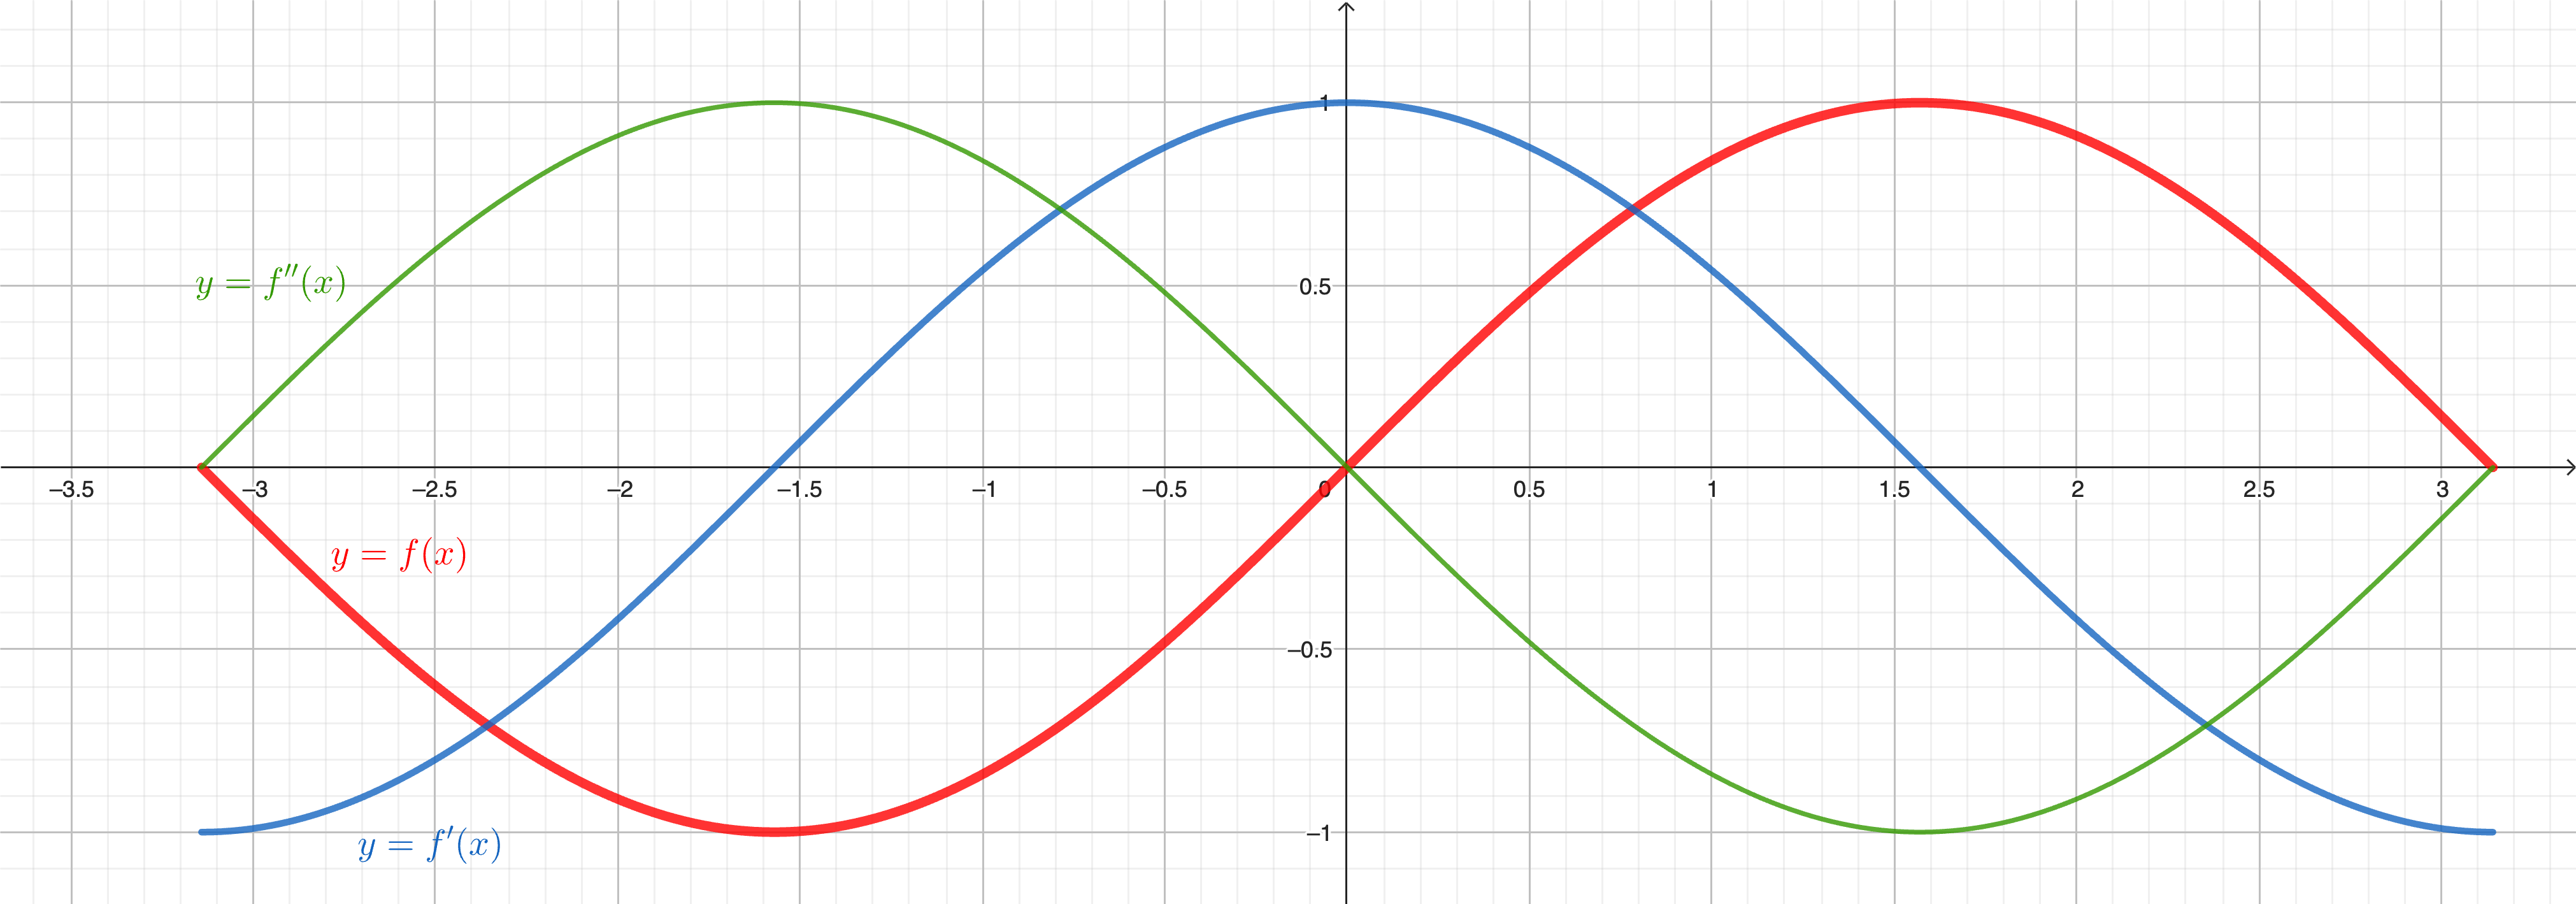
\includegraphics[width=.8\textwidth]{pics/concavidad-convexidad-seno.png}}

    La derivada segunda de $f$ es $f''(x)=-\sen(x)$. Tenemos que $f''(x)>0$ en $(-\pi,0)$ y $f''(x)<0$ en $(0,\pi)$. Por lo tanto
    \begin{itemize}
        \item $f$ es convexa en $[-\pi,0]$.
        \item $f$ es cóncava en $[0,\pi]$.
        \item $x=0$ es un punto de inflexión de $f$.
    \end{itemize}
\end{example}

\begin{example}
    Consideremos ahora el problema de hallar el punto de una curva $y=$que está más cercano a un punto dado, que está fuera de la curva.
    Consider
\end{example}
\begin{example}
    Consideremos ahora la función $f(x)$ de la cual sólo tenemos la gráfica de su derivada:

    \noindent
    \begin{minipage}{.5\textwidth}
        Observamos que $f'(x)>0$ en $(a,c)$ y que $f'(x)<0$ en $(c,d)$. Luego
        \begin{itemize}
            \item $f$ es creciente en $[a,c]$.
            \item $f$ es decreciente en $[c,d]$.
        \end{itemize}
        Observamos también que $f'(x)$ es creciente en $[a,b]$ y decreciente en $[b,d]$. Luego
        \begin{itemize}
            \item $f$ es convexa en $[a,b]$.
            \item $f$ es cóncava en $[b,d]$.
            \item Hay un punto de inflexión en $x=b$.
        \end{itemize}
        \end{minipage}
    \begin{minipage}{.5\textwidth}
        \centering
        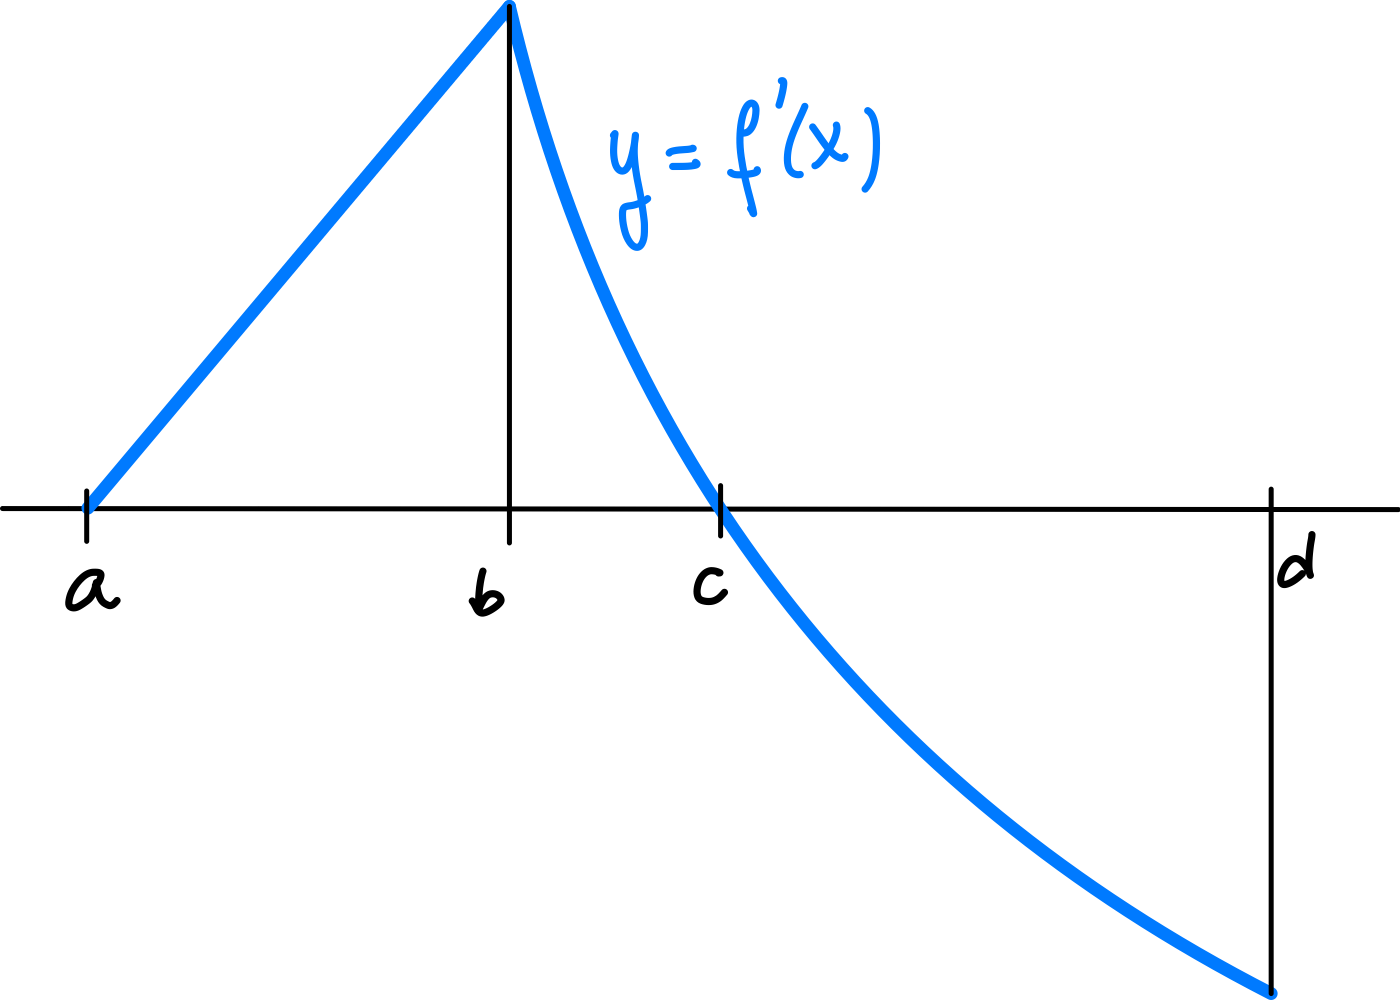
\includegraphics[width=.9\textwidth]{pics/f-prima-ej-1.png}
    \end{minipage}
\end{example}

\subsubsection*{Ejercicios de la sección~\getcurrentref{chapter}.\getcurrentref{section}}

\begin{enumerate}

\item Hallar el mínimo de la función $f:(0,+\infty)\to \R$ dada por $\D f(x) = x + \frac1x$.

\item Hallar las dimensiones del cilindro circular recto de volumen $V$ que tenga mínima área exterior. (Si el cilindro tiene base circular de radio $r$ y altura $h$, entonces el volumen es: $\pi \, r^2\, h$ y el área exterior es $2\pi \, r^2 + 2 \pi \, r\, h$).

\item Consideremos la función $(x-1)^2+(x-3)^2+(x-5)^2$. Graficarla en Geogebra, y encontrar el valor mínimo y el punto mínimo.

\item Dados $a_1<a_2<\dots <a_n$, hallar el valor de $x$ que minimiza $\sum_{i=1}^n (a_i-x)^2$.

\item La siguientes figuras muestran la gráfica de \emph{la derivada $f'$ de $f$}. Hallar:
\begin{itemize}
  \item Todos los puntos máximos y mínimos locales de $f$.
  \item Intervalos de crecimiento y decrecimiento de $f$.
  \item Intervalos de convexidad y concavidad de $f$, y puntos de inflexión.
\end{itemize} 

\begin{multicols}{2}
  \begin{enumerate}
    \item 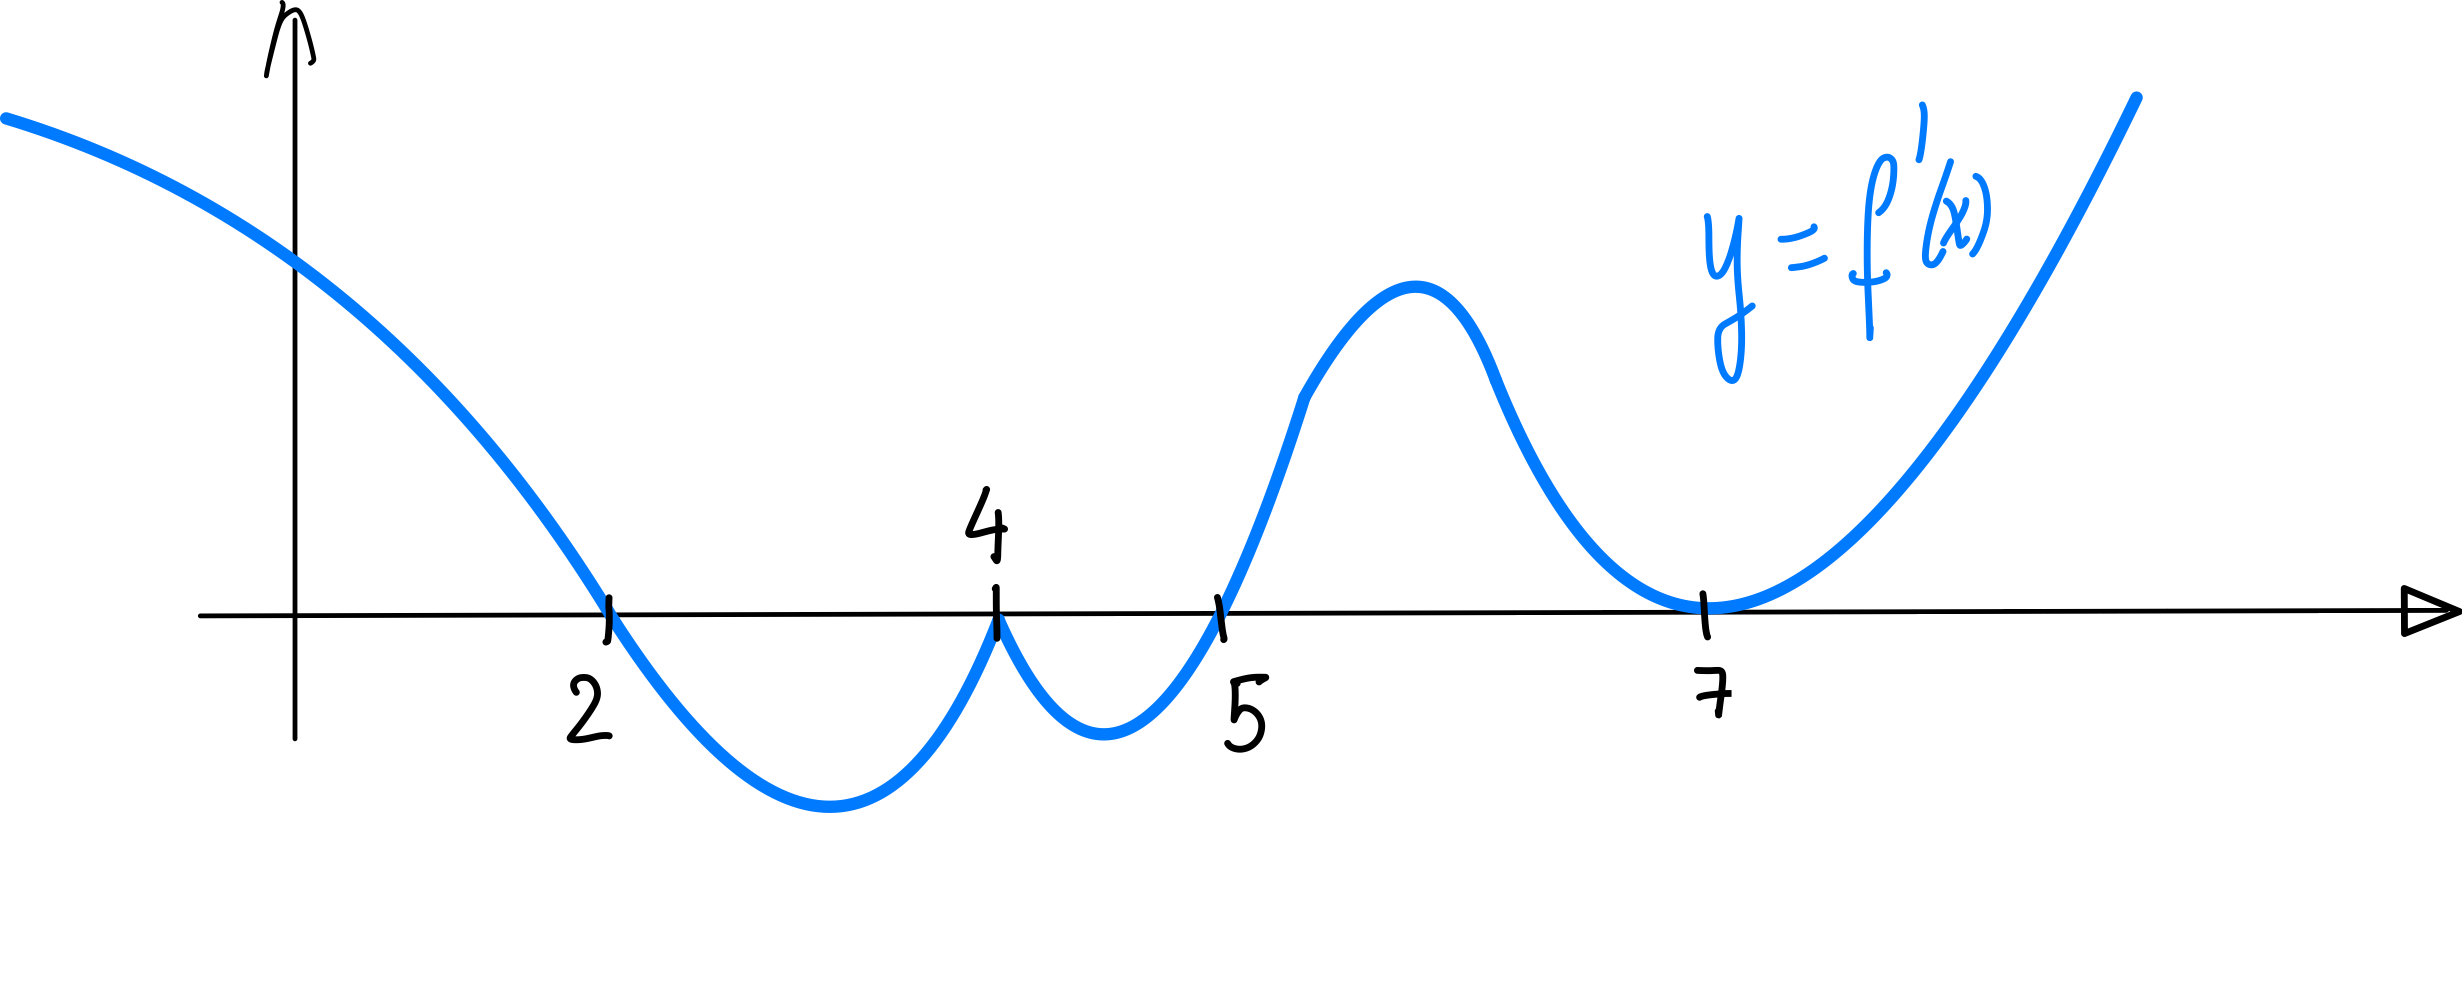
\includegraphics[width=.4\textwidth]{pics/max-min-locales-ej-a.png}
    \item 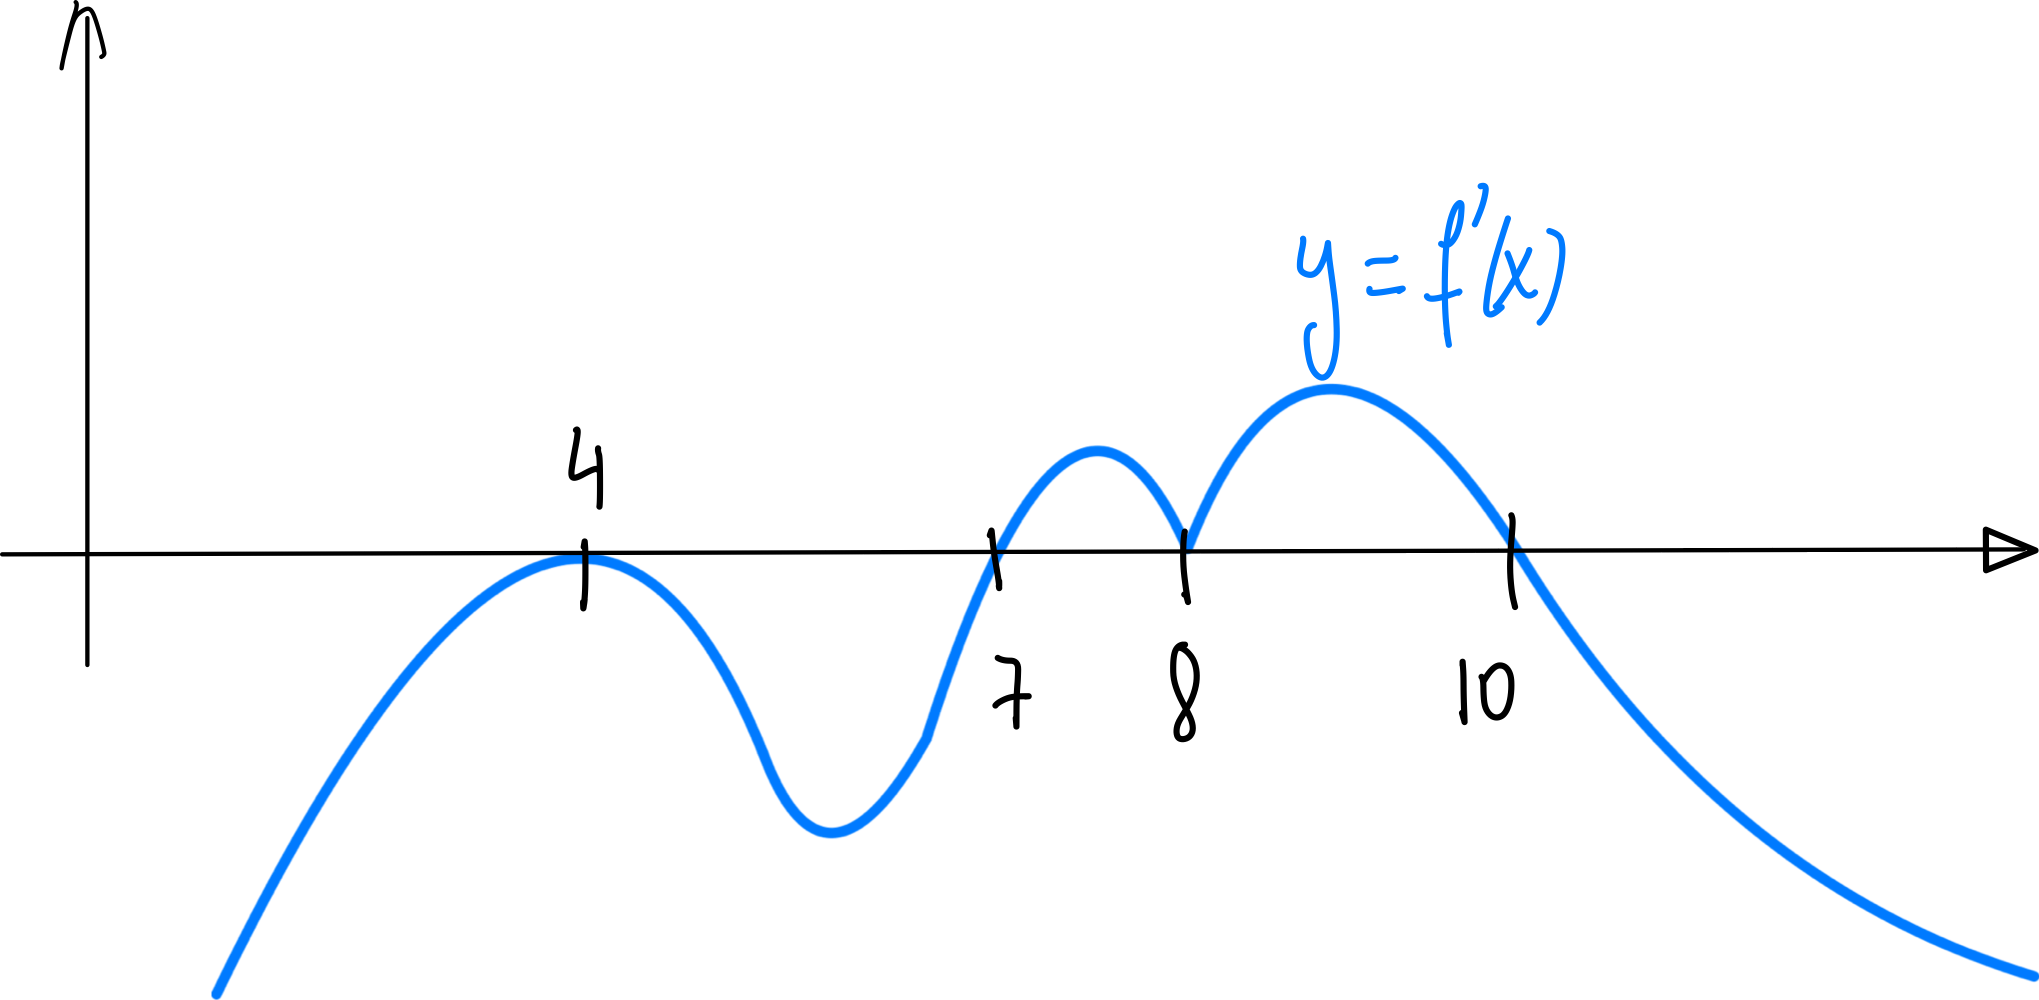
\includegraphics[width=.4\textwidth]{pics/max-min-locales-ej-b.png}
    \item 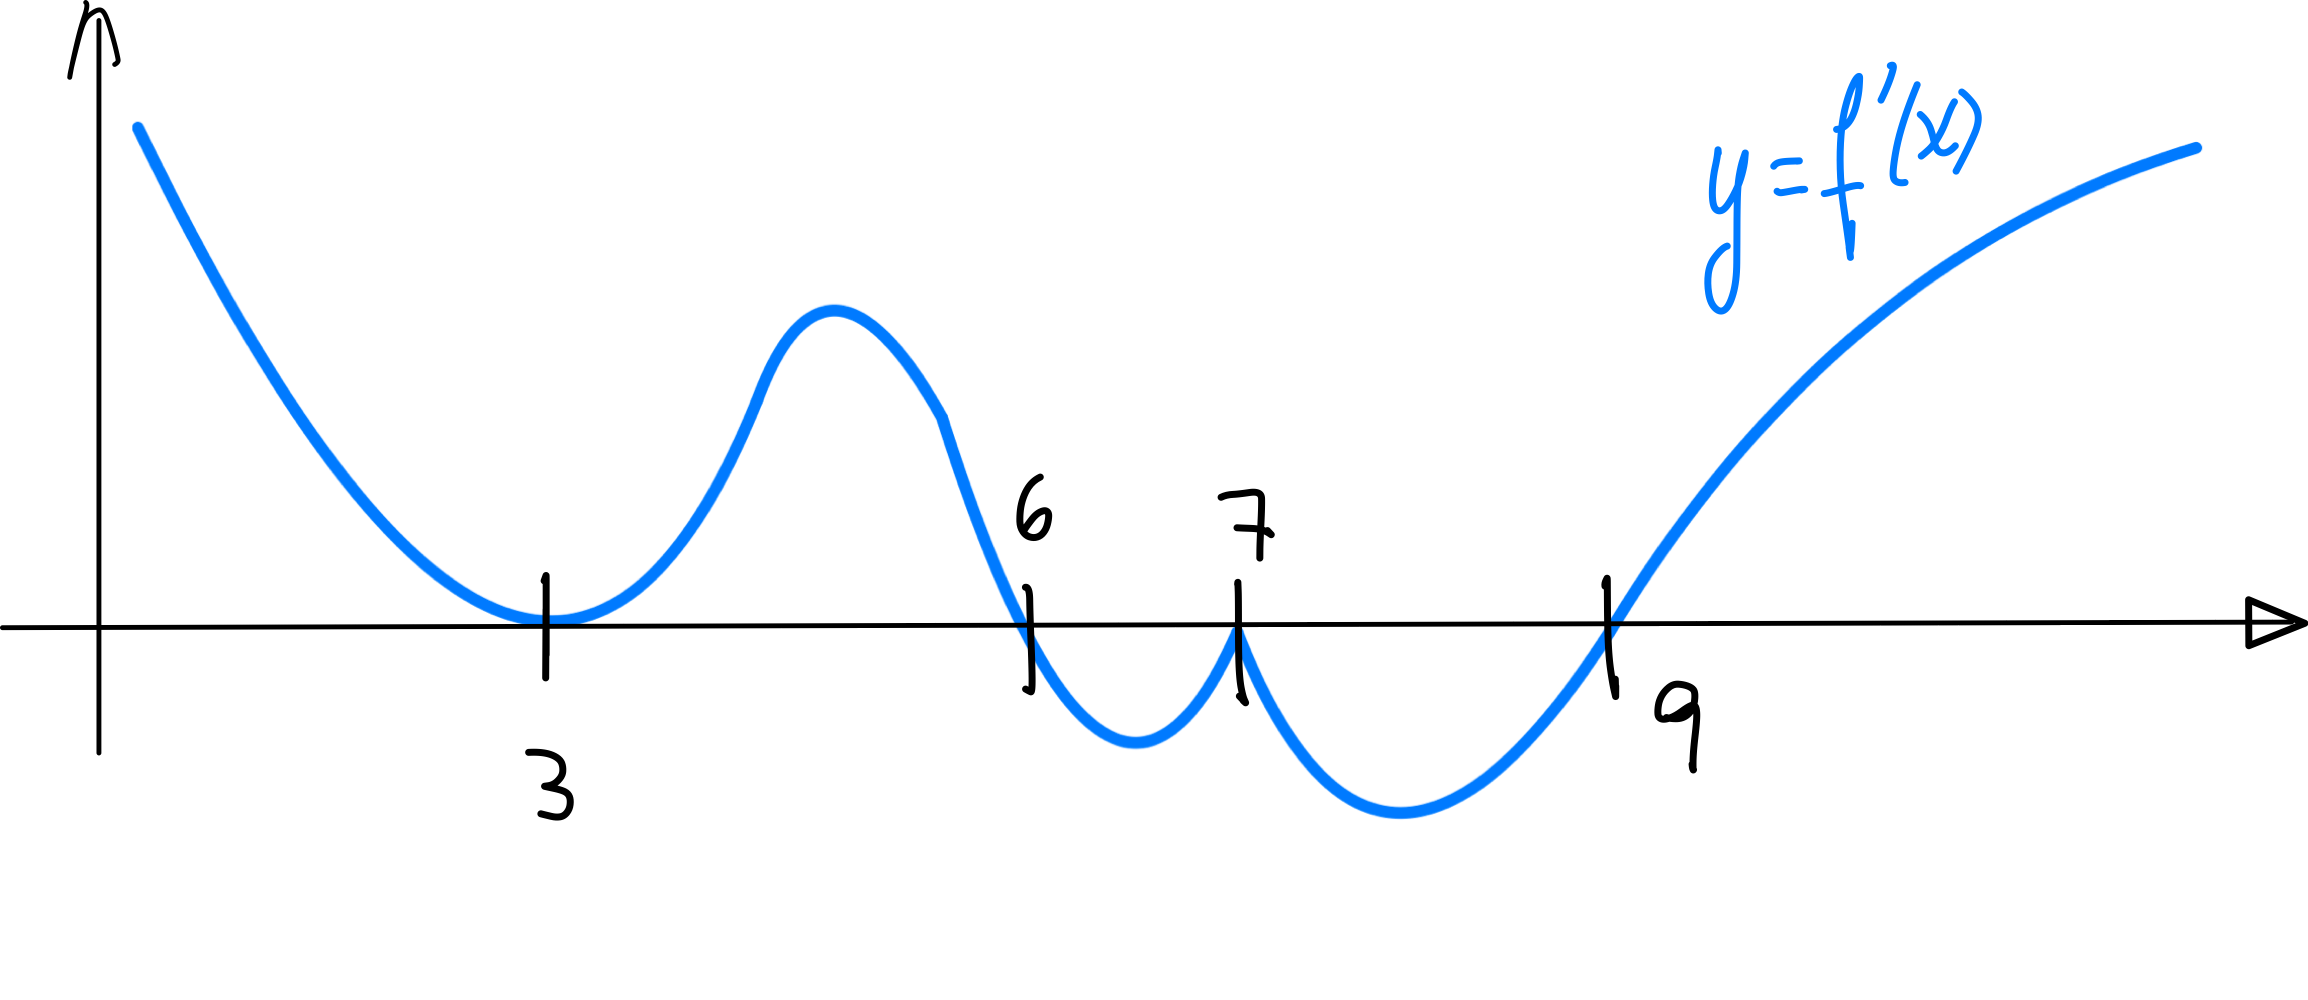
\includegraphics[width=.4\textwidth]{pics/max-min-locales-ej-c.png}
    \item 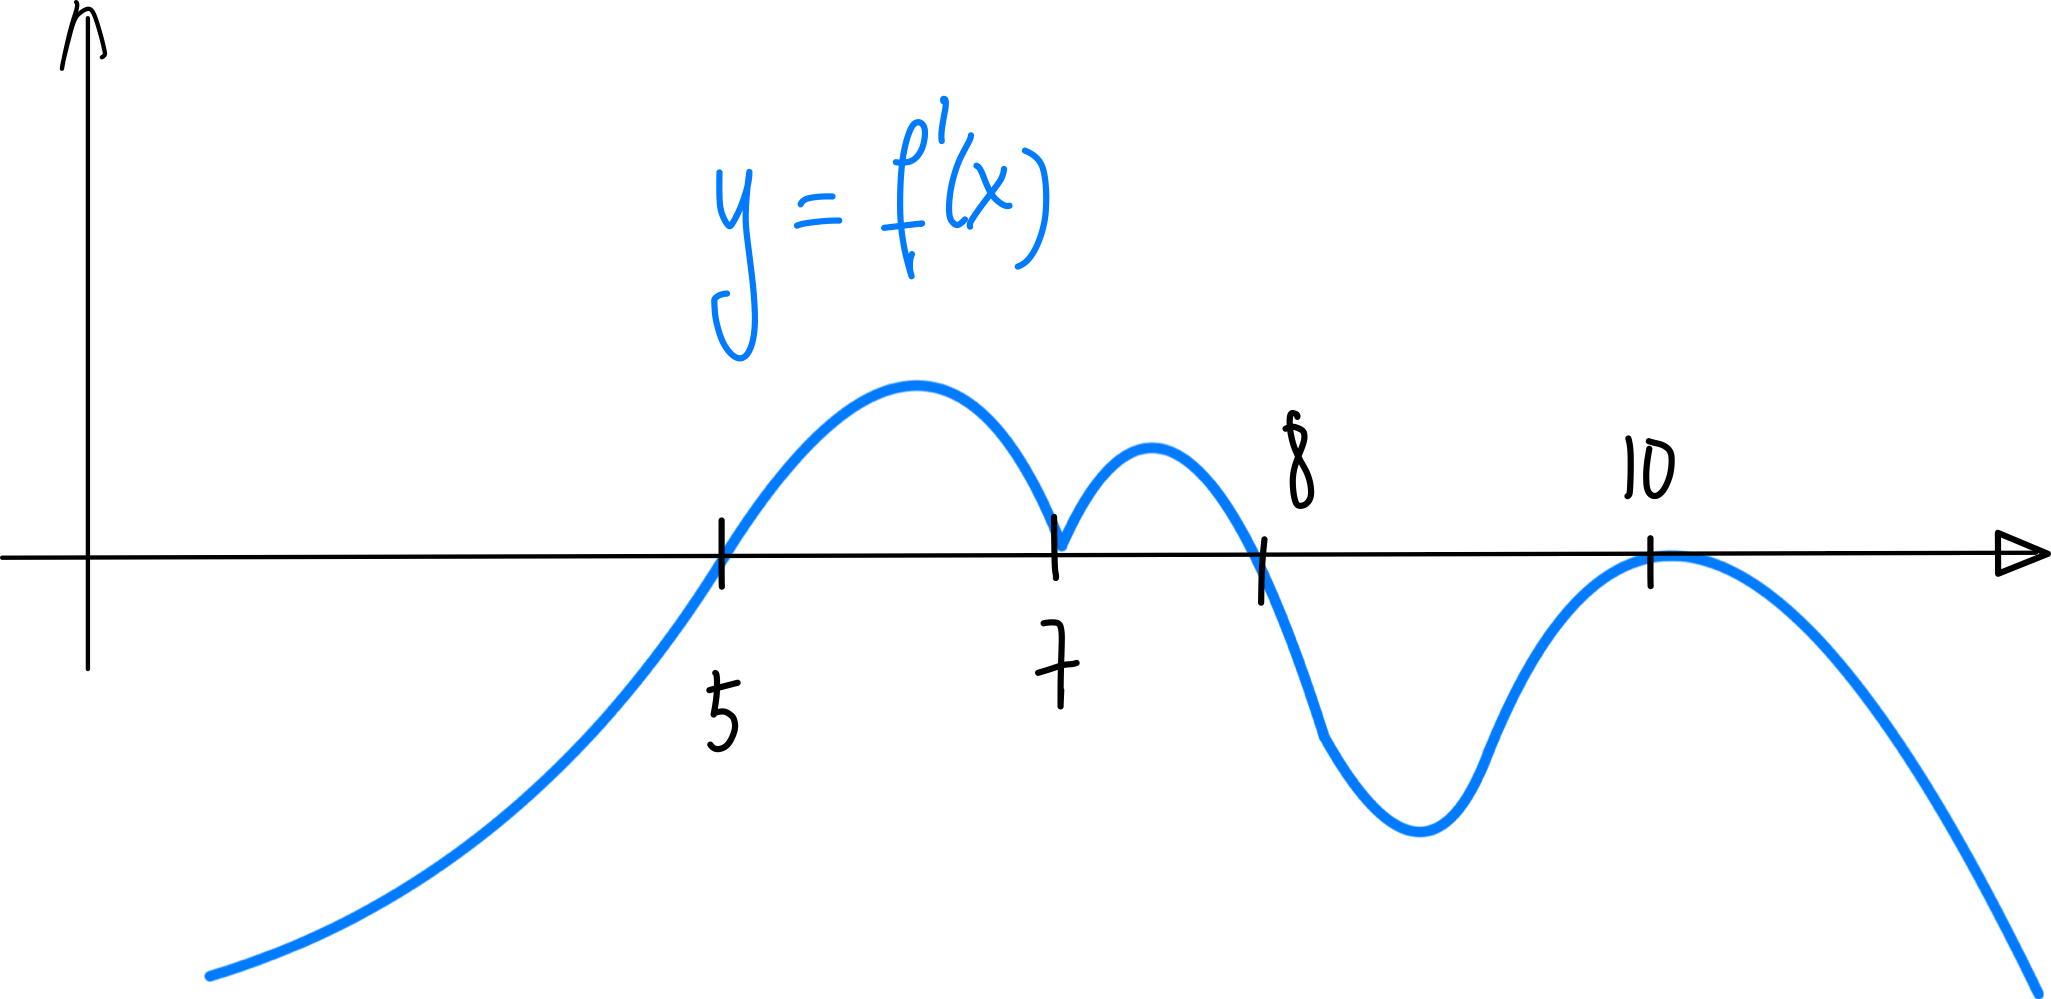
\includegraphics[width=.4\textwidth]{pics/max-min-locales-ej-d.png}
  \end{enumerate}
  
\end{multicols}

\end{enumerate}


\section{Regla de L'Hospital}

\begin{comment}
Vemos ahora un Teorema del Valor Medio Generalizado:
\begin{theorem}[Teorema del Valor Medio Generalizado (de Cauchy)]
    Si $f$ y $g$ son continuas en $[a,b]$ y derivables en $(a,b)$, entonces existe $c\in(a,b)$ tal que
    \[
        \big( f(b)-f(a) \big) \cdot g'(c) = \big( g(b)-g(a) \big)\cdot f'(c).
    \]
    Si, además $g'(x)\neq 0$ para todo $x\in(a,b)$, entonces
    \[
    \frac{f(b)-f(a)}{g(b)-g(a)}=\frac{f'(c)}{g'(c)}.
    \]
\end{theorem}

\begin{proof}
    Consideremos la función
    \[
    h(x) = \big( f(b)-f(a) \big) \cdot \big(g(x)-g(a)\big) 
    - \big( g(b)-g(a) \big)\cdot \big(f(x)-f(a)\big).
    \]
    Esta función $h(x)$ es continua en $[a,b]$ y derivable en $(a,b)$ por ser producto y suma de funciones de ese tipo. Además:
    \begin{align*}
        h(a) &= \big( f(b)-f(a) \big) \cdot \big(g(a)-g(a)\big) 
        - \big( g(b)-g(a) \big)\cdot \big(f(a)-f(a)\big) = 0,
        \\
        h(b) &= \big( f(b)-f(a) \big) \cdot \big(g(b)-g(a)\big) 
        - \big( g(b)-g(a) \big)\cdot \big(f(b)-f(a)\big) = 0.
    \end{align*}
    Entonces $h$ satisface las hipótesis del Teorema de Rolle, y existe $c\in(a,b)$ tal que $h'(c)=0$. Pero
    \[
        h'(x) = \big( f(b)-f(a) \big) \cdot g'(x)
        - \big( g(b)-g(a) \big)\cdot f'(x).
    \]
    Luego, $\D \big( f(b)-f(a) \big) \cdot g'(c)
    - \big( g(b)-g(a) \big)\cdot f'(c)= 0$, que es lo que se quería demostrar.
\end{proof}

Como consecuencia de este teorema, vemos un resultado que nos da una igualdad de mucha utilidad para el cálculo de límites.


\begin{proposition}[Regla de L'Hospital, caso $0/0$]
    Sean $f$ y $g$ funciones definidas y derivables en un intervalo $(a,b)$.
    Para $x_0\in(a,b)$, supongamos que $g'(x)\neq 0$, para todo $x\neq x_0$ y $f(x_0)=g(x_0)=0$.
    Bajo estas hipótesis, si existe $\D\limxo \frac{f'(x)}{g'(x)}=\ell$, entonces existe $\D\limxo \frac{f(x)}{g(x)}$ y además $\D\limxo \frac{f(x)}{g(x)}=\ell$, es decir
    \[
        \limxo \frac{f(x)}{g(x)}=\limxo \frac{f'(x)}{g'(x)}.
    \]
\end{proposition}

\begin{proof}
    Sea $\ell = \limxo \frac{f'(x)}{g'(x)}=\ell$. Entonces, dado $\epsilon>0$, existe $\delta>0$ tal que
    \[
    0<|x-x_0|<\delta\quad\implies\quad \Big| \frac{f'(x)}{g'(x)}-\ell \Big|<\epsilon.\]
    Ahora bien, para cada $x$ tal que $0<|x-x_0|<\delta$, existe $c$ entre $x$ y $x_0$, tal que
    \[
    \frac{f(x)}{g(x)}=\frac{f(x)-f(x_0)}{g(x)-g(x_0)} = \frac{f'(c)}{g'(c)}.
    \]
    Como $c$ está entre $x$ y $x_0$, resulta que $0<|c-x_0|<|x-x_0|<\delta$, y entonces
    \[
    \Big| \frac{f(x)}{g(x)}-\ell\Big| 
    = 
    \Big| \frac{f'(c)}{g'(c)}-\ell\Big| < \epsilon.
    \]
    Hemos demostrado entonces que, dado $\epsilon>0$, existe $\delta>0$ tal que
    \[
        \Big| \frac{f(x)}{g(x)}-\ell\Big| <\epsilon,
        \quad\text{para todo $x$ tal que $0<|x-x_0|<\delta$}.
    \]    
    Es decir, $\D\limxo \frac{f(x)}{g(x)}=\ell$.
\end{proof}

\end{comment}

El siguiente teorema nos da una igualdad de mucha utilidad para el cálculo de límites:

\begin{proposition}[Regla de L'Hospital, caso $0/0$]
    Sean $f$ y $g$ funciones definidas y derivables en un intervalo $(a,b)$.
    Supongamos que para $x_0\in(a,b)$ queremos calcular $\D\limxo \frac{f(x)}{g(x)}$, pero $f(x_0)=\limxo f(x)=0$ y $g(x_0)=\limxo g(x)=0$, es decir, tenemos un indeterminado del tipo $\frac00$.
    Supongamos también que $f'$ y $g'$ son continuas en $(a,b)$.
    Si $g'(x_0)\neq 0$, entonces existe $\D\limxo \frac{f(x)}{g(x)}$ y además $\D\limxo \frac{f(x)}{g(x)}=\frac{f'(x_0)}{g'(x_0)}$, es decir
    \[
        \limxo \frac{f(x)}{g(x)}=\frac{f'(x_0)}{g'(x_0)}=\limxo \frac{f'(x)}{g'(x)}.
    \]
\end{proposition}

\begin{proof}
    Recordemos primero que $\D\limxo \frac{f(x)}{g(x)}=\limho \frac{f(x_0+h)}{g(x_0+h)}$. Y por la definición alternativa de derivada~\eqref{eq:derivada-o(h)}
    \begin{align*}
        f(x_0+h) &= \underbrace{f(x_0)}_{0} + h \cdot f'(x_0) + o(h) = h \cdot f'(x_0) + o(h),\\
        g(x_0+h) &= \underbrace{g(x_0)}_{0} + h \cdot g'(x_0) + o(h) = h \cdot g'(x_0) + o(h).
    \end{align*}
    Luego
    \begin{align*}
        \frac{f(x_0+h)}{g(x_0+h)} &= \frac{ h \cdot f'(x_0) + o(h)}{h \cdot g'(x_0) + o(h)}
        = \frac hh  \cdot \frac{ f'(x_0) + \frac{o(h)}h}{ g'(x_0) + \frac{o(h)}h}
        \toh{0} \frac{f'(x_0) + 0}{g'(x_0) + 0}
        = \frac{  f'(x_0)}{ g'(x_0)}.
    \end{align*}
    Es decir, $\D\limxo \frac{f(x)}{g(x)}=\frac{f'(x_0)}{g'(x_0)}=\limxo \frac{f'(x)}{g'(x)}$.
\end{proof}
    
\begin{example}
    Utilizaremos esta regla para calcular $\D\lim_{x\to 1} \frac{\ln x}{x-1}$.
    El numerador y el denominador tienden a $0$ cuando $x\to1$:
    \[
        \lim_{x\to 1} \ln x = \ln 1 = 0,
        \qquad
        \lim_{x\to 1} (x-1) = 1-1=0.
    \]
    Por lo tanto es un límite indeterminado de la forma $\frac00$. Si derivamos el numerador y el denominador tenemos
    \[
    \frac{d \ln x}{dx} = \frac1x\tox{1}1, \qquad \frac{d(x-1)}{dx}=1\tox{1}1.
    \]
    Calculamos ahora el límite del cociente de estas dos derivadas:
    \[
        \lim_{x\to 1} \frac{\ln x}{x-1}= \lim_{x\to 1} \frac{\frac{d \ln x}{dx}}{\frac{d(x-1)}{dx}}
    =\lim_{x\to 1} \frac{\frac1x}{1}=\lim_{x\to 1} \frac1x=1.
    \]
\end{example}

\begin{example}
    La regla de L'Hospital puede aplicarse de manera repetida. Por ejemplo, para calcular $\D\lim_{x\to 0}\frac{1-\cos x}{x^2}$ que otra vez es del tipo $\frac00$, observamos que 
    \[
    \dd[]{(1-\cos x)}{x}=0-(-\sen x)=\sen x,
    \quad\text{y}\quad
    \dd[]{x^2}{x}=2x.
    \]
    Ambas derivadas tienden a cero cuando $x\to 0$, por lo tanto seguimos teniendo un \emph{indeterminado}. Volvemos a derivar
    \[
        \dd[]{\sen x}{x}=\cos x,
        \quad\text{y}\quad
        \dd[]{(2x)}{x}=2.
    \]
    Estas nuevas derivadas tienden a $1$ y a $2$, respectivamente, cuando $x\to 0$, por lo tanto, $\D\lim_{x\to 0}\frac{1-\cos x}{x^2}=\frac12$. Todo este razonamiento es muy complicado de escribir de esta manera.
    
    Una manera más sencilla de escribirla es la siguiente:
    \[
        \lim_{x\to 0}\frac{1-\cos x}{x^2}
        \eqLH \lim_{x\to 0}\frac{\sen x}{2x}
        \eqLH \lim_{x\to 0}\frac{\cos x}{2} = \frac12.
    \]
    Donde usamos \,$\eqLH$\, para indicar que en ese paso estamos usando la regla de L'Hospital.
\end{example}


\begin{proposition}[Regla de L'Hospital, caso $\infty/\infty$]
    Sean $f$ y $g$ funciones definidas y derivables en un intervalo $(a,b)$.
    Para $x_0\in(a,b)$, supongamos que $\limxo f(x)=\limxo g(x)=\infty$.
    Bajo estas hipótesis, si existe $\D\limxo \frac{f'(x)}{g'(x)}=\ell$, entonces existe $\D\limxo \frac{f(x)}{g(x)}$ y además $\D\limxo \frac{f(x)}{g(x)}=\ell$, es decir
    \[
        \limxo \frac{f(x)}{g(x)}=\limxo \frac{f'(x)}{g'(x)}.
    \]
\end{proposition}

La demostración de esta proposición y las que siguen a continuación quedan fuera del alcance de este apunte, y serán discutidas en los \emph{Coloquios de Demostraciones}.

\begin{proposition}[Regla de L'Hospital, 2$^{\text{do}}$ caso $0/0$]
    Sean $f$ y $g$ funciones definidas y derivables en un intervalo $(a,b)$.
    Para $x_0\in(a,b)$, supongamos que $g'(x)\neq 0$, para todo $x\neq x_0$ y $f(x_0)=g(x_0)=0$.
    Bajo estas hipótesis,
    \[
    \text{si}\quad \D\limxo \frac{f'(x)}{g'(x)}=\infty
    \quad\text{entonces}\quad
    \D\limxo \frac{f(x)}{g(x)}=\infty.
    \]
\end{proposition}

\begin{proposition}[Regla de L'Hospital, 2$^{\text{do}}$ caso $\infty/\infty$]
    Sean $f$ y $g$ funciones definidas y derivables en un intervalo $(a,b)$.
    Para $x_0\in(a,b)$, supongamos que $\limxo f(x)=\limxo g(x)=\infty$.
    Bajo estas hipótesis, 
    \[
    \text{si}\quad \D\limxo \frac{f'(x)}{g'(x)}=\infty
    \quad\text{entonces}\quad
    \D\limxo \frac{f(x)}{g(x)}=\infty.
    \]
\end{proposition}

La regla de L'Hospital también puede aplicarse a los casos en que la variable $x$ tiende a infinito (en lugar de a $x_0$). Veamos su aplicación en dos ejemplos:

\begin{example}
    Calculemos $\D\lim_{x\to+\infty} \frac{\ln x}x$. Tanto el numerador como el denominador tienden a $\infty$ cuando $x\to+\infty$, así que es posible aplicar la regla de L'Hospital:
    \[
        \lim_{x\to+\infty} \frac{\ln x}x 
        \eqLH \lim_{x\to+\infty} \frac{1/x}1 
        = \lim_{x\to+\infty} \frac1x = 0.
    \]
\end{example}

\begin{example}
    Calculemos $\D\lim_{x\to+\infty} \frac{x^3}{e^x}$. Tanto el numerador como el denominador tienden a $\infty$ cuando $x\to+\infty$, así que es posible aplicar la regla de L'Hospital:
    \[
        \lim_{x\to+\infty} \frac{x^3}{e^x}
        \eqLH
        \lim_{x\to+\infty} \frac{3x^2}{e^x}
        \eqLH
        \lim_{x\to+\infty} \frac{6x}{e^x}
        \eqLH
        \lim_{x\to+\infty} \frac{6}{e^x}
        = 0.
    \]
    En base a este ejemplo, vemos que por inducción podemos probar que,
    cualquiera sea $n\in\N$,
    $\D\lim_{x\to+\infty} \frac{x^n}{e^x}=0$. En palabras, se dice que $e^x$ \emph{tiende a infinito más rápido que cualquier potencia de $x$}.
\end{example}


\subsubsection*{Ejercicios de la sección~\getcurrentref{chapter}.\getcurrentref{section}}

\begin{enumerate}
\item Calcular los siguientes límites:
\begin{multicols}{2}
  \begin{enumerate}
    \item $\D \lim_{x\to 0} \frac{x-\sen x}{x^3}$
    \item $\D \lim_{x\to 2} \frac{x^2-4}{x-2}$
    \item $\D \lim_{x\to a} \frac{x^2-a^2}{x-a} $
    \item $\D \lim_{x\to 0} \frac{\sen (5x)}x$
    \item $\D \lim_{x\to 1} \frac{x^2-2x+1}{3x^2+2x-5} $
    \item $\D \lim_{x\to 0} \frac{e^{2x}-e^{-2x}-4x}{x-\sen x}$
    \item $\D \lim_{x\to a} \frac{x^n-a^n}{x-a}$
    \item $\D \lim_{x\to 0} \frac{\tan x-x}{x-\sen x}$
    \item $\D \lim_{x\to \frac\pi2} \frac{\ln(\sen x)}{\pi -2x}$
    \item $\D \lim_{x\to a} \frac{\sen x - \sen a}{x-a}$
    \item $\D \lim_{x\to 0} \frac{(a+x)^x-a^x}{x^2}$ ($a>0$)
    \item $\D \lim_{x\to +\infty} \frac{\ln x}{x^2}$
    \item $\D \lim_{x\to +\infty} \frac{\ln x}{x^{0.1}}$
    \item $\D \lim_{x\to +\infty} \frac{e^x}{x^n}$ (\niN)
    \item $\D \lim_{x\to +\infty} \frac{e^x}{\sqrt{x}}$
    \item $\D \lim_{x\to +\infty} \frac{x+\ln x}{x\, \ln x}$
    \item $\D \lim_{x\to +\infty} \frac{\ln x}{e^x}$
    \item $\D \lim_{x\to +\infty} \frac{\sen (1/x)}{1/x}$
    \item $\D \lim_{x\to 0^+} x^2 \, \ln x$
    \item $\D \lim_{x\to 0^+} (x-\sen x) \, \ln x$
    \item $\D \lim_{x\to 0} \big( \frac1x-\frac{\cos x}{\sen x}\big)$
  \end{enumerate}
\end{multicols}

\item Para calcular $\D\limxo f(x)^{g(x)}$ en los casos de indeterminación ($1^\infty$, $0^0$, $\infty^0$) suele ser útil calcular el logaritmo del límite:
\[
\ln \big(\limxo f(x)^{g(x)}\big) = \limxo \ln \big(f(x)^{g(x)}\big)
= \limxo \big[ g(x) \, \ln f(x) \big] = \limxo \frac{\ln f(x)}{1/g(x)}.
\]
Para aplicar este último límite puede ser útil aplicar L'Hospital. Si se encuentra el límite $\ell$, luego el límite original será $e^\ell$.

Aplicar este procedimiento apra calcular los siguientes límites:
\begin{multicols}{2}
  \begin{enumerate}
    \item $\D \lim_{x\to 0}x^{\sen x}$
    \item $\D \lim_{x\to +\infty}\big(1+\frac ax)^x$
    \item $\D \lim_{x\to +\infty}(1+x)^{1/x}$
    \item $\D \lim_{x\to 0^+} (-\ln x)^x$
    \item $\D \lim_{x\to 0^+} \Big(\frac{\tan x}x\Big)^{1/x^2} $
    \item $\D \lim_{x\to \pi/2} (\sen x)^{\tan x}$
    \item $\D \lim_{x\to +\infty} \Big(\frac{\ln x}{x}\Big)^{1/x}$
    \item $\D \lim_{x\to 0} x^x$
    \item $\D \lim_{x\to 0} x^{x^x}$
  \end{enumerate}
\end{multicols}

\item Calcular primero los límites siguientes sin utilizar L'Hospital.
?`Qué ocurre si se intenta aplicar L'Hospital?
\begin{multicols}{2}
  \begin{enumerate}
    \item $\D \lim_{x\to 0}\frac{x^2\,\sen(1/x)}{\sen x}$
    \item $\D \lim_{x\to +\infty}\frac{x+\sen x}{x+\cos x}$
  \end{enumerate}
\end{multicols}
Volver a interpretar el Teorema de L'Hospital en vistas de estas observaciones.


\end{enumerate}


% \section{Estudio de funciones}


% \subsubsection*{Ejercicios de la sección~\getcurrentref{chapter}.\getcurrentref{section}}

% \begin{enumerate}
% \item 
% \end{enumerate}



\subsection*{Ejercicios del capítulo~\getcurrentref{chapter}}




\begin{enumerate}
    \item Calcular las siguientes derivadas usando la definición:
\begin{multicols}{2}
    \begin{enumerate}
        \item $f'(1)$ para $f(x)=2x+3$
        \item $f'(2)$ para $f(x)=3x^2-1$
        \item $f'(4)$ para $f(x)=\sqrt{x}$
        \item $f'(2)$ para $f(x)=1/x$
    \end{enumerate}
\end{multicols}
\item Determinar si la siguiente función es derivable en $x_0=0$:
\[
    f(x) = \begin{cases} x^2 \sen \frac1x,\quad&\text{si $x\neq 0$},
    \\
    0, \quad&\text{si $x=0$}.
\end{cases}
\]
\item Hallar usando la definición, la derivada de $f:(0,+\infty)\to R$ dada por $f(x)=\sqrt{x}$.
Plantear el cociente incremental y multiplicar por \emph{el conjugado}.
    \item Hallar $f'(x)$ siendo $f(x)$ igual a:
\begin{multicols}{2}
\begin{enumerate}
    \item $\D 3x^3+6x^2-2x+1$
    \item $\D x(3+x^2)$
    \item $\D 4x(2+x^3+5x^4)$
    \item $\D (x+2)(x+3)(3x+1)(2+5x^2)$
    \item $\D \frac{x-1}x$
    \item $\D \frac{4x-3}{2x+4}$
    \item $\D \frac{(x+3)^2(4x-1)}{(2x+1)^2(3x-2)}$
    \item $\D \frac{x^3}{(4-x^2)^2}$
    \item $\D 4x-\frac2x$
\end{enumerate}
\end{multicols}

\item Calcular las siguientes derivadas:
\begin{multicols}{2}
\begin{enumerate}
    \item $\D \dd[3]{}{x} \big(3x^3+6x^2-2x+1\big)$
    \item $\D \dd[4]{}{x}\big(x(3+x^2)\big)$
    \item $\D \dd[2]{}{x}\big((x+2)(x+3)(3x+1)(2+5x^2)\big)$
    \item $\D \dd[2]{}{x}\frac{x-1}x$
\end{enumerate}
\end{multicols}

\item Sea $f(x)=x^n$, para \niN. Hallar $f^{(k)}(x)$, para
\begin{multicols}{3}
    \begin{enumerate}
    \item $k=n$;
    \item $k>n$;
    \item $k<n$.
\end{enumerate}
\end{multicols}

\item Dada la función polinómica $\D p(x)=a_n x^n + a_{n-1} x^{n-1} + \dots + a_1 x + a_0$:
\begin{multicols}{2}
    \begin{enumerate}
    \item Hallar $\D \dd[n]{p(x)}{x}$;
    \item Hallar $\D \dd[k]{p(x)}{x}$, para $k>n$.
\end{enumerate}
\end{multicols}


    \item Hallar $f'(x)$ siendo $f(x)$ igual a:
\begin{multicols}{2}
\begin{enumerate}
    \item $\D \tan x$
    \item $\D \cotan x$
    \item $\D \sec x$
    \item $\D \cosec x$
    \item $\D \frac{x+e^x}{5-x^2}+\tan x$
    \item $\D x \ln x$
\end{enumerate}
\end{multicols}

\item Se definen las funciones hiperbólicas de la siguiente manera:
\[
\cosh x = \frac{e^x+e^{-x}}{2},
\qquad
\senh x = \frac{e^x-e^{-x}}{2}
\]
\begin{enumerate}
    \item Probar que $\cosh^2 x-\senh^2 x = 1$
    \item Probar que $\D\dd{\senh x}{x} = \cosh x$
    \item Probar que $\D\dd{\cosh x}{x} = \senh x$
\end{enumerate}

\item Hallar una fórmula para la derivada de $\log_a x$.

\item Hallar las siguientes derivadas:
\begin{multicols}{2}
    \begin{enumerate}
        \item $\D\dd[2]{\sen x}{x}$
        \item $\D\dd[2]{\cos x}{x}$
        \item $\D\dd[2]{\senh x}{x}$
        \item $\D\dd[2]{\cosh x}{x}$
    \end{enumerate}
\end{multicols}


\item Hallar las siguientes derivadas, para \niN:
\begin{multicols}{2}
    \begin{enumerate}
        \item $\D\dd[n]{\sen x}{x}$
        \item $\D\dd[n]{\cos x}{x}$
        \item $\D\dd[n]{\senh x}{x}$
        \item $\D\dd[n]{\cosh x}{x}$
    \end{enumerate}
\end{multicols}
    \item Hallar $f'(x)$ siendo $f(x)$ igual a:
\begin{multicols}{2}
\begin{enumerate}
    \item $\D \sqrt{2x^2+3}$
    \item $\D \sqrt{6x^2-3x-2}$
    \item $\D (x^2+1)\sqrt{x^2+1}$
    \item $\D \frac{x^3}{(4-x^2)^3}$
    \item $\D \sqrt{x^2+a^2}$
    \item $\D \frac{a^2}{\sqrt{a^2-x^2}}$
    \item $\D \tan \frac{x^2+2x-1}{(x^2+3)^2}$
    \item $\D \sen\big(\sen(\cos x)\big)$
    \item $\D e^{\sen x}+e^{\tan x}$
    \item $x \sen x+\sqrt[3]{x^2}$
    \item $\D \sen(3x^3-1) \, (4x^2+7)$
    \item $\D e^{\sen x} + e^{\tan x}$
    \item $\D x^3\ln x+e^{x^2}$
    \item $\D \frac{\ln(x+2)}{x+2}$
    \item $\D \big(\ln x\big)^3$
    \item $\D \ln (x^3)$
    \item $\D \ln \frac{\sqrt x-\sqrt a}{\sqrt x+\sqrt a}$
    \item $\D \frac{x^3}{\ln x}$
    \item $\D x^{3x}$
    \item $\D (2^x)^x$
    \item $\D (x^2+1)^{\sqrt x}$
    \item $\D x^{x^x}$
\end{enumerate}
\end{multicols}

    \item * Si $f:\R\to\R$ es continua en $\R$ y derivable en todo punto de $\R\setminus\{a\}$, y existe $\D\lim_{x\to a}f'(x)= \ell$, entonces $f$ es derivable en $x=a$ y $f'(a) = \ell$.
Usar el Teorema del Valor Medio (de Lagrange) para calcular las derivadas laterales.

\item Probar las siguientes afirmaciones para una función $f:[a,b]\to \R$ continua en $[a,b]$ y derivable en $(a,b)$:
\begin{enumerate}
  \item Si $f'(x)\ge 0$ para todo $x\in(a,b)$, entonces $f$ es creciente en $[a,b]$; es decir, $a\le x_1<x_2\le b$ implica $f(x_1)\le f(x_2)$.
  \item Si $f$ es creciente, entonces $f'(x)\ge 0$ para todo $x\in(a,b)$.
  \item Si $f'(x)\le 0$ para todo $x\in(a,b)$, entonces $f$ es decreciente en $[a,b]$; es decir, $a\le x_1<x_2\le b$ implica $f(x_1)\ge f(x_2)$
  \item Si $f$ es decreciente, entonces $f'(x)\le 0$ para todo $x\in(a,b)$.
\end{enumerate}

\item Encontrar un ejemplo de una función $f:\R\to\R$ que sea estrictamente creciente y derivable, pero que no cumpla que $f'(x)>0$, para todo $x\in\R$.

\item Probar que la función $f(x)=\sqrt[3]{(x-3)^2}$ satisface $f(1)=f(5)$ pero no existe $c\in(1,5)$ tal que $f'(c)=0$. ?`Por qué no se puede aplicar el Teorema de Rolle?

\item Sea $f(x)=(x-1)\, x\, (x+2)\, (x+5)$. Probar que $f'(x)$ tiene tres raíces reales.

\item Para cada una de las siguientes funciones, determinar el punto $c\in(0,1)$ que cumple el Teorema del Valor Medio en el intervalo $[0,1]$:
\begin{multicols}{3}
  \begin{enumerate}
    \item $f(x)=3x$;
    \item $f(x)=2x^2$;
    \item $f(x)=\sqrt[3]{x}$.
  \end{enumerate}
\end{multicols}

\item Hallar $f'(x)$ para:
\begin{multicols}{2}

  \begin{enumerate}
    \item $\D f(x) = \arcsen(\sqrt x)$;
    \item $\D f(x) = \arccos(x^2+1)$;
    \item $\D f(x) = \big(e^{\arcsen (1/x)}\big)^x$;
    \item $\D f(x) = \sqrt[3]{\arccos\Big(\frac{x^2}{1+x^2}\Big)}$;
    \item $\D f(x) = \ln\big(\arccos (x)\big)$;
  \end{enumerate}
  
\end{multicols}
    
\item Hallar el mínimo de la función $f:(0,+\infty)\to \R$ dada por $\D f(x) = x + \frac1x$.

\item Hallar las dimensiones del cilindro circular recto de volumen $V$ que tenga mínima área exterior. (Si el cilindro tiene base circular de radio $r$ y altura $h$, entonces el volumen es: $\pi \, r^2\, h$ y el área exterior es $2\pi \, r^2 + 2 \pi \, r\, h$).

\item Consideremos la función $(x-1)^2+(x-3)^2+(x-5)^2$. Graficarla en Geogebra, y encontrar el valor mínimo y el punto mínimo.

\item Dados $a_1<a_2<\dots <a_n$, hallar el valor de $x$ que minimiza $\sum_{i=1}^n (a_i-x)^2$.

\item La siguientes figuras muestran la gráfica de \emph{la derivada $f'$ de $f$}. Hallar:
\begin{itemize}
  \item Todos los puntos máximos y mínimos locales de $f$.
  \item Intervalos de crecimiento y decrecimiento de $f$.
  \item Intervalos de convexidad y concavidad de $f$, y puntos de inflexión.
\end{itemize} 

\begin{multicols}{2}
  \begin{enumerate}
    \item 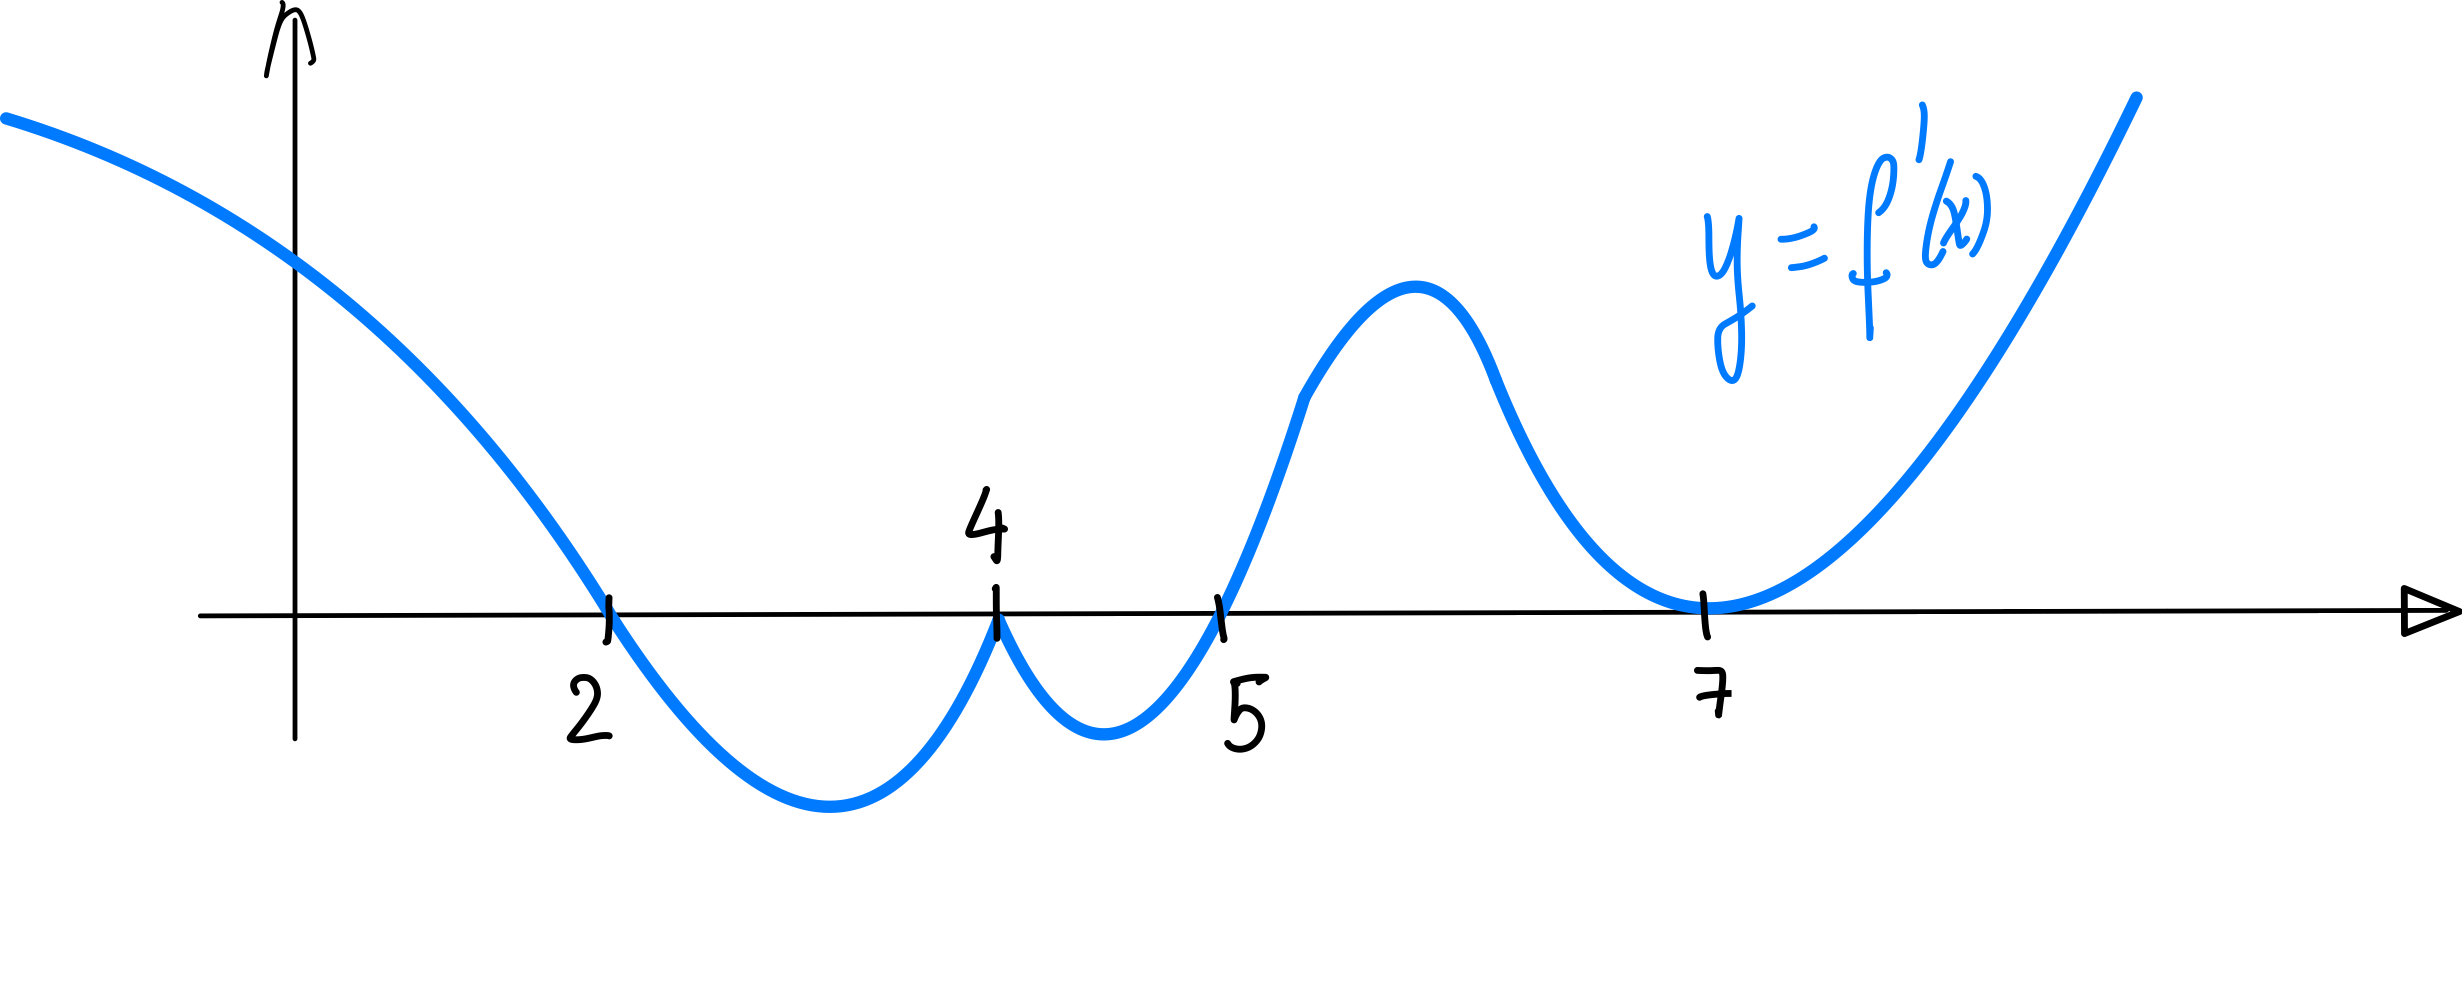
\includegraphics[width=.4\textwidth]{pics/max-min-locales-ej-a.png}
    \item 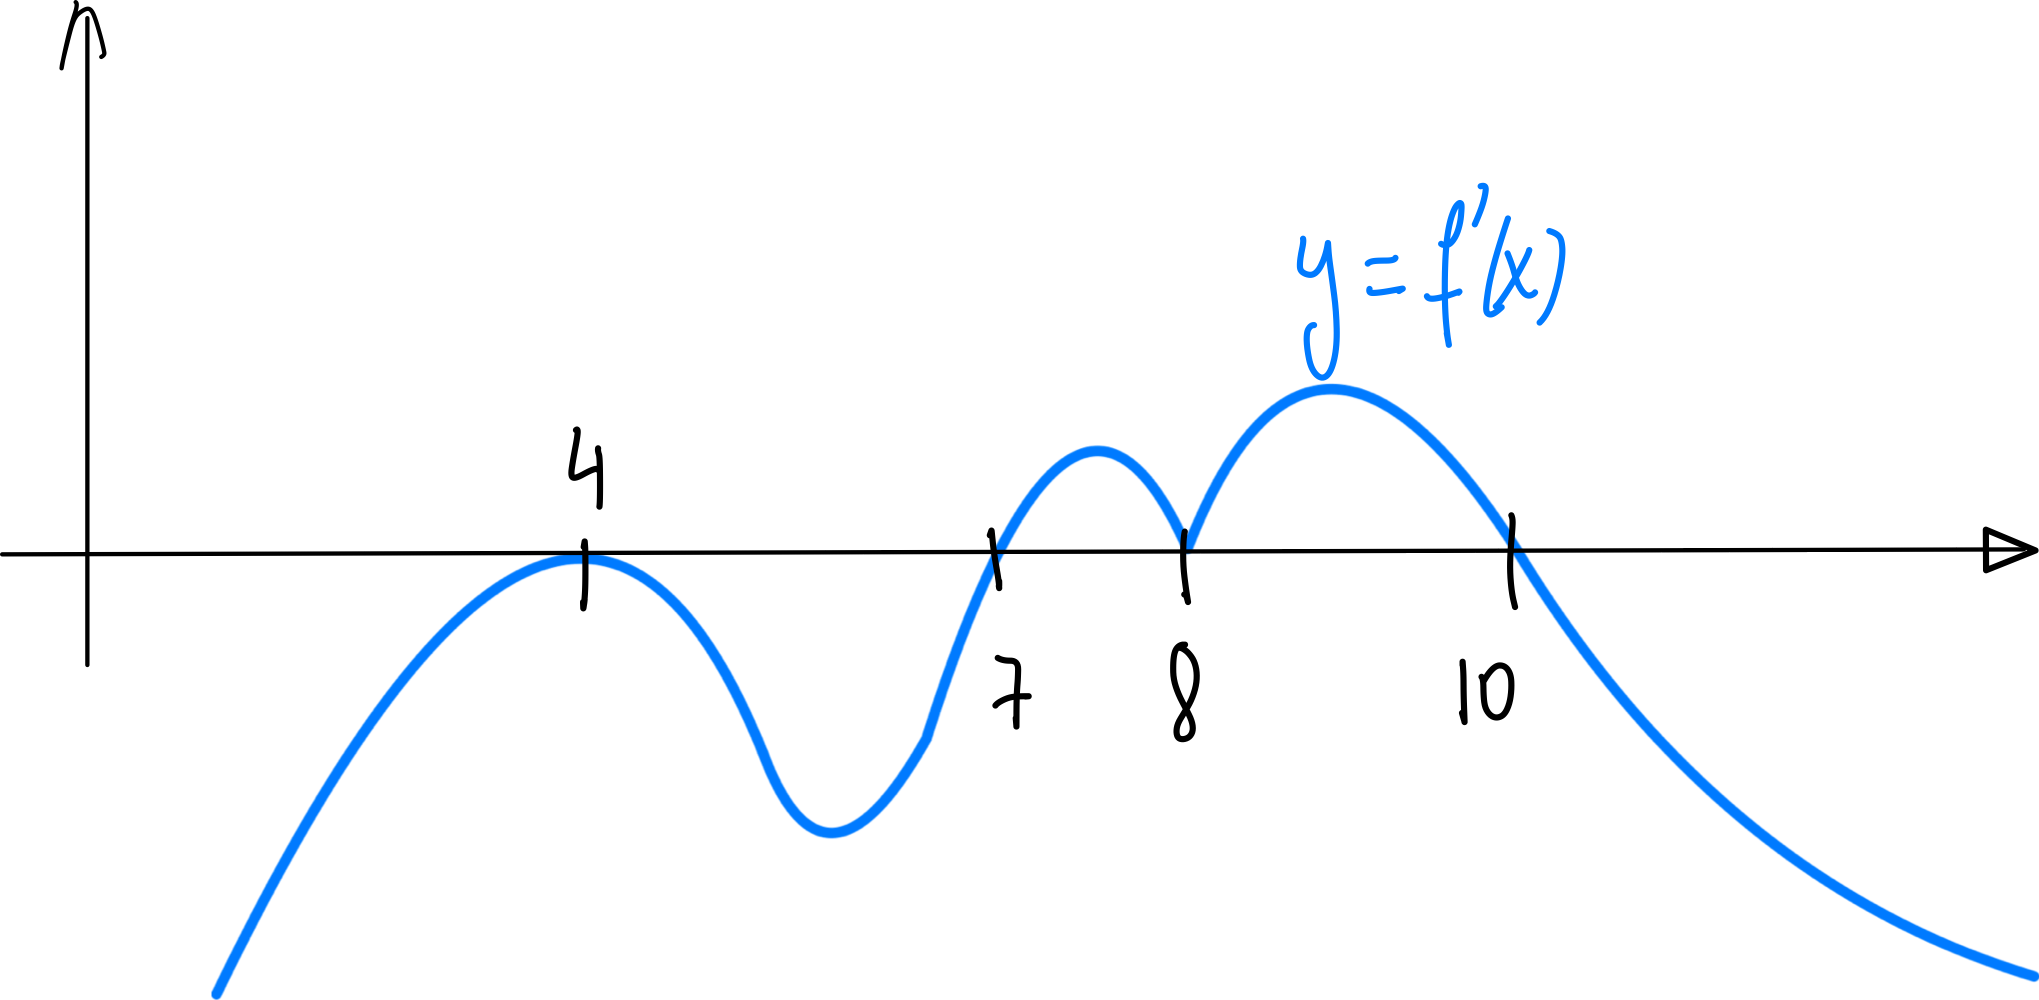
\includegraphics[width=.4\textwidth]{pics/max-min-locales-ej-b.png}
    \item 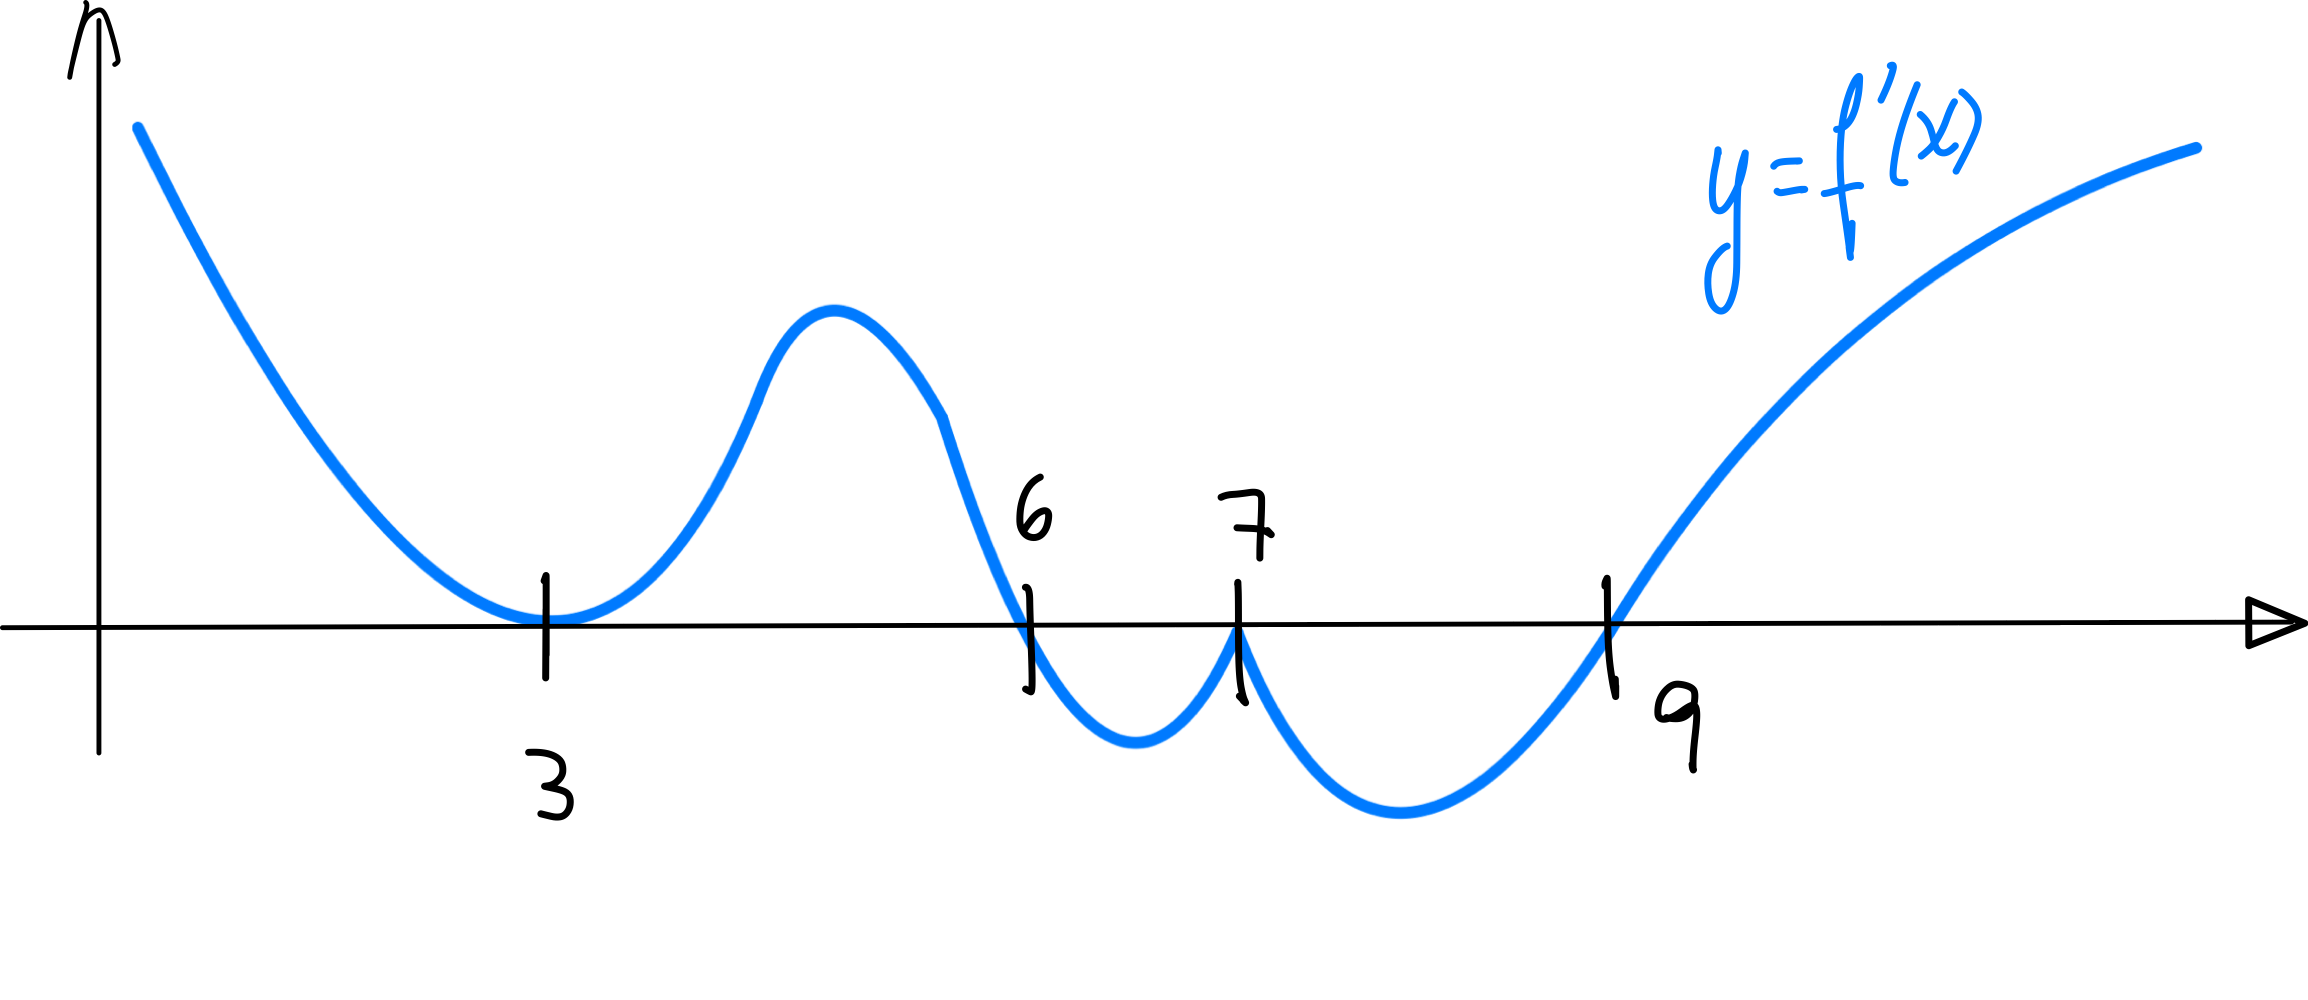
\includegraphics[width=.4\textwidth]{pics/max-min-locales-ej-c.png}
    \item 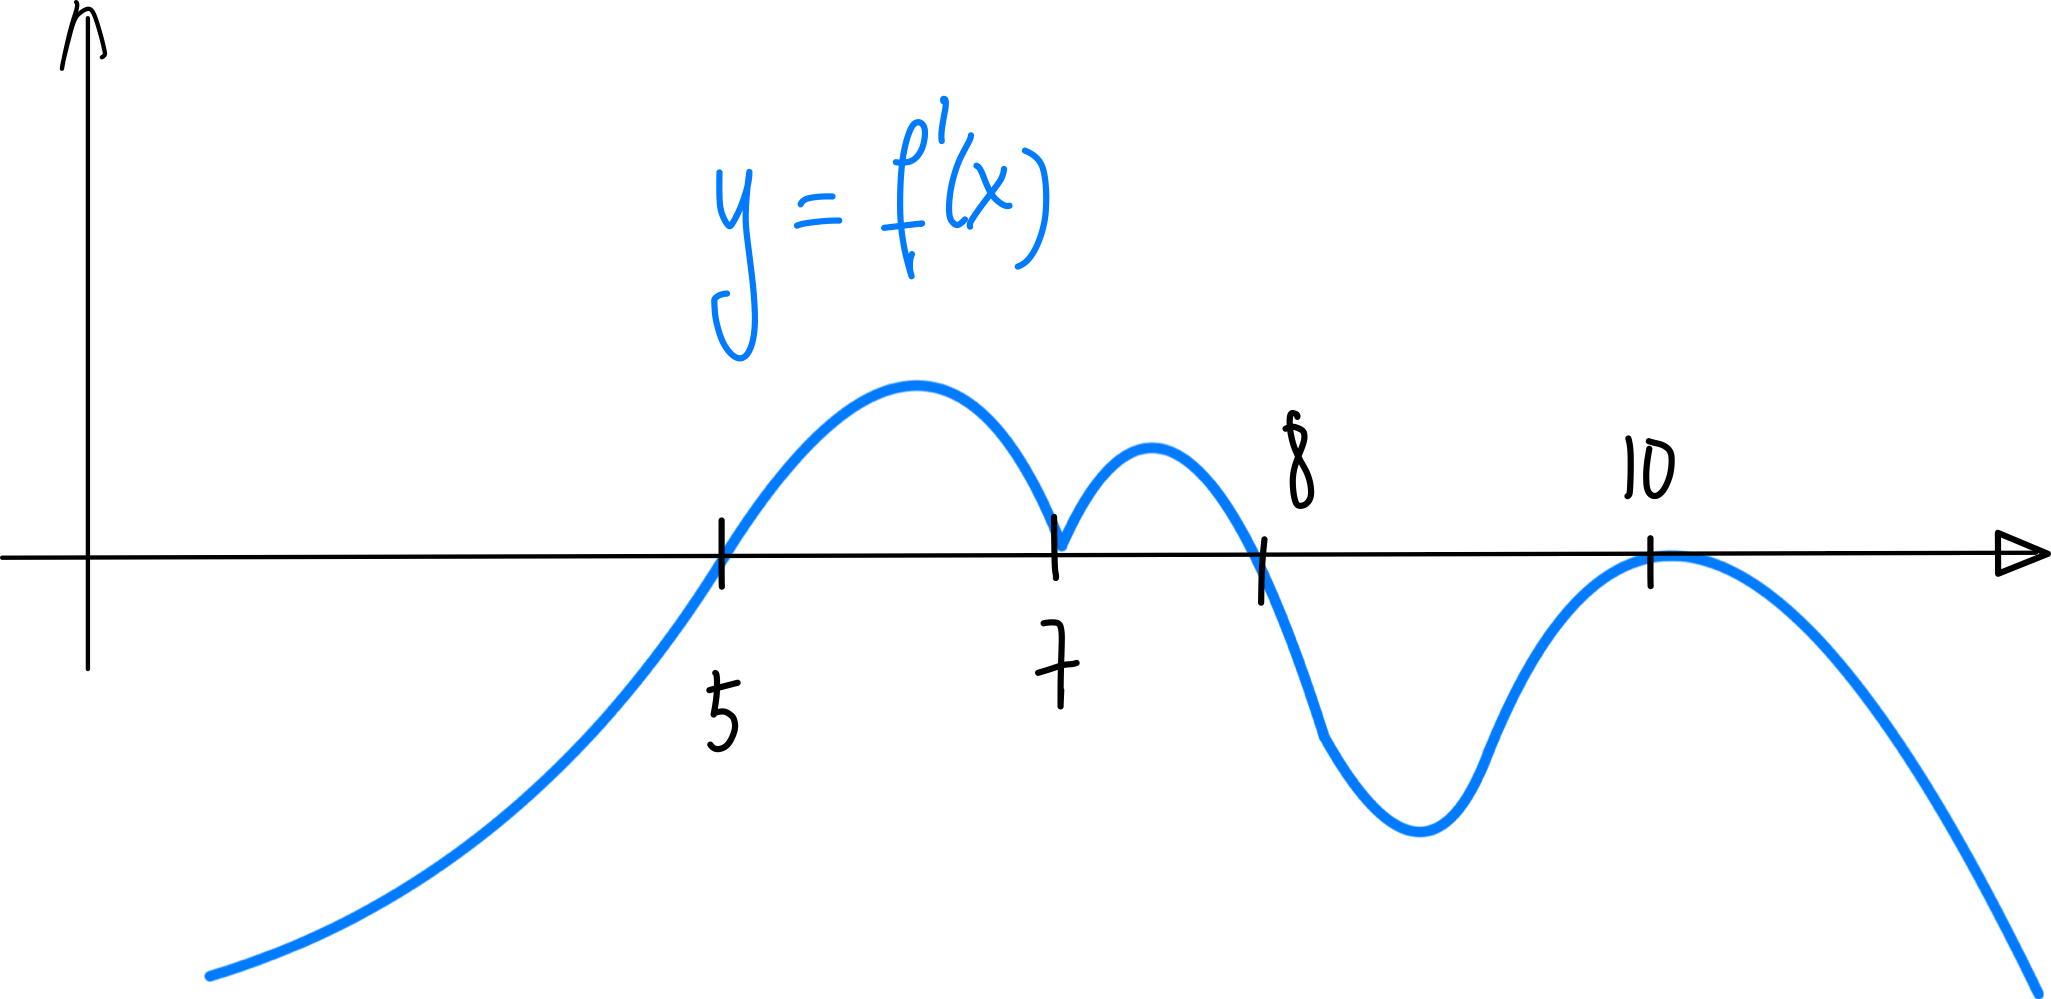
\includegraphics[width=.4\textwidth]{pics/max-min-locales-ej-d.png}
  \end{enumerate}
  
\end{multicols}

    \item Calcular los siguientes límites:
\begin{multicols}{2}
  \begin{enumerate}
    \item $\D \lim_{x\to 0} \frac{x-\sen x}{x^3}$
    \item $\D \lim_{x\to 2} \frac{x^2-4}{x-2}$
    \item $\D \lim_{x\to a} \frac{x^2-a^2}{x-a} $
    \item $\D \lim_{x\to 0} \frac{\sen (5x)}x$
    \item $\D \lim_{x\to 1} \frac{x^2-2x+1}{3x^2+2x-5} $
    \item $\D \lim_{x\to 0} \frac{e^{2x}-e^{-2x}-4x}{x-\sen x}$
    \item $\D \lim_{x\to a} \frac{x^n-a^n}{x-a}$
    \item $\D \lim_{x\to 0} \frac{\tan x-x}{x-\sen x}$
    \item $\D \lim_{x\to \frac\pi2} \frac{\ln(\sen x)}{\pi -2x}$
    \item $\D \lim_{x\to a} \frac{\sen x - \sen a}{x-a}$
    \item $\D \lim_{x\to 0} \frac{(a+x)^x-a^x}{x^2}$ ($a>0$)
    \item $\D \lim_{x\to +\infty} \frac{\ln x}{x^2}$
    \item $\D \lim_{x\to +\infty} \frac{\ln x}{x^{0.1}}$
    \item $\D \lim_{x\to +\infty} \frac{e^x}{x^n}$ (\niN)
    \item $\D \lim_{x\to +\infty} \frac{e^x}{\sqrt{x}}$
    \item $\D \lim_{x\to +\infty} \frac{x+\ln x}{x\, \ln x}$
    \item $\D \lim_{x\to +\infty} \frac{\ln x}{e^x}$
    \item $\D \lim_{x\to +\infty} \frac{\sen (1/x)}{1/x}$
    \item $\D \lim_{x\to 0^+} x^2 \, \ln x$
    \item $\D \lim_{x\to 0^+} (x-\sen x) \, \ln x$
    \item $\D \lim_{x\to 0} \big( \frac1x-\frac{\cos x}{\sen x}\big)$
  \end{enumerate}
\end{multicols}

\item Para calcular $\D\limxo f(x)^{g(x)}$ en los casos de indeterminación ($1^\infty$, $0^0$, $\infty^0$) suele ser útil calcular el logaritmo del límite:
\[
\ln \big(\limxo f(x)^{g(x)}\big) = \limxo \ln \big(f(x)^{g(x)}\big)
= \limxo \big[ g(x) \, \ln f(x) \big] = \limxo \frac{\ln f(x)}{1/g(x)}.
\]
Para aplicar este último límite puede ser útil aplicar L'Hospital. Si se encuentra el límite $\ell$, luego el límite original será $e^\ell$.

Aplicar este procedimiento apra calcular los siguientes límites:
\begin{multicols}{2}
  \begin{enumerate}
    \item $\D \lim_{x\to 0}x^{\sen x}$
    \item $\D \lim_{x\to +\infty}\big(1+\frac ax)^x$
    \item $\D \lim_{x\to +\infty}(1+x)^{1/x}$
    \item $\D \lim_{x\to 0^+} (-\ln x)^x$
    \item $\D \lim_{x\to 0^+} \Big(\frac{\tan x}x\Big)^{1/x^2} $
    \item $\D \lim_{x\to \pi/2} (\sen x)^{\tan x}$
    \item $\D \lim_{x\to +\infty} \Big(\frac{\ln x}{x}\Big)^{1/x}$
    \item $\D \lim_{x\to 0} x^x$
    \item $\D \lim_{x\to 0} x^{x^x}$
  \end{enumerate}
\end{multicols}

\item Calcular primero los límites siguientes sin utilizar L'Hospital.
?`Qué ocurre si se intenta aplicar L'Hospital?
\begin{multicols}{2}
  \begin{enumerate}
    \item $\D \lim_{x\to 0}\frac{x^2\,\sen(1/x)}{\sen x}$
    \item $\D \lim_{x\to +\infty}\frac{x+\sen x}{x+\cos x}$
  \end{enumerate}
\end{multicols}
Volver a interpretar el Teorema de L'Hospital en vistas de estas observaciones.


\end{enumerate}

\chapter{Integración}

En este capítulo vamos a estudiar el concepto que, junto con el de derivada, forma el núcleo del cálculo diferencial e integral.
Veremos que dicho concepto, el de \emph{integral}, será definido por motivos totalmente ajenos a los que nos llevaron a definir la derivada, pero también veremos que está íntimamente conectado a través del teorema fundamental del cálculo.

\section{La integral definida de una función continua}
% Seguimos el Salas-Hille

La noción de integral definida como la presentaremos aquí aparece naturalmente cuando se intenta resolver el problema del cálculo del área de una región plana. El lector recordará la fórmula del área de ciertas figuras planas, por ejemplo el rectángulo el triángulo, el círculo, etc.

\centerline{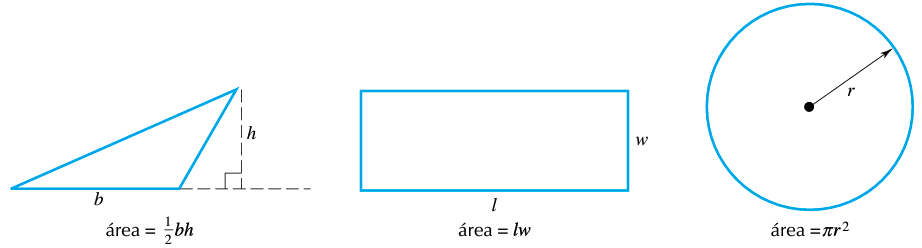
\includegraphics[width=.8\textwidth]{pics/areas-simples.png}}

En este capítulo veremos cómo calcular el área de figuras más generales. Comenzaremos con el cálculo del área que queda delimitada de la siguiente manera:

\noindent
\begin{minipage}{.5\textwidth}
  \begin{itemize}
  \item Por debajo, por el eje $x$;
  \item Por encima, por la gráfica de $y=f(x)$;
  \item A la izquierda por la recta $x=a$; 
  \item A la derecha por la recta $x=b$.
\end{itemize}
\end{minipage}
\begin{minipage}{.5\textwidth}
  \centering
  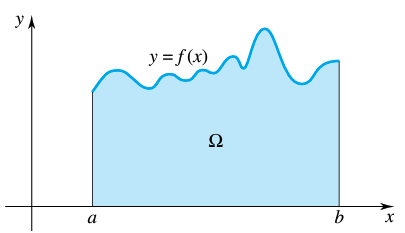
\includegraphics[width=.9\textwidth]{pics/area-bajo-curva.png}
\end{minipage}

\noindent
\begin{minipage}{.5\textwidth}
  Consideramos ahora una subdivisión del intervalo $[a,b]$ en un número finito de subintervalos que no se solapan:
  \[
  [x_0,x_1],\ [x_1,x_2],\dots,\ [x_{n-1},x_n]
  \]
  con $\D a=x_0<x_1<\dots<x_n=b$.

  Observamos que el área de la región $\Omega$ es lo mismo que la suma de las áreas de las regiones $\Omega_i$.
\end{minipage}
\begin{minipage}{.5\textwidth}
  \centering
  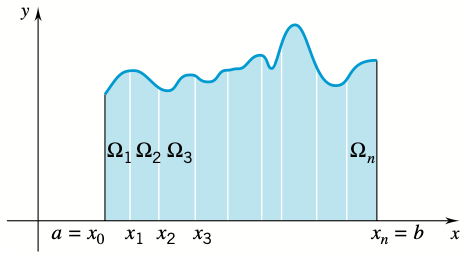
\includegraphics[width=.9\textwidth]{pics/area-bajo-curva-particionada.png}
\end{minipage}

Podemos aproximar el área total de $\Omega$ aproximando el área de cada una de las subregiones $\Omega_i$ y sumando los resultados.
Definimos, para cada $i=1,2,\dots,n$ las siguientes cantidades:
\[ 
  m_i = \min_{x\in [x_{i-1},x_i]}f(x)=\min_{[x_{i-1},x_i]}f,
  \qquad
  M_i = \max_{x\in [x_{i-1},x_i]}f(x)=\max_{[x_{i-1},x_i]}f.
\]
Luego, si $r_i = [x_{i-1},x_i]\times [0,m_i]$ y $R_i = [x_{i-1},x_i]\times [0,M_i]$, resulta que
\[
r_i \subset \Omega_i \subset R_i
\quad\text{y entonces}\quad
\area(r_i)\le \area(\Omega_i) \le \area(R_i).
\]

\centerline{
  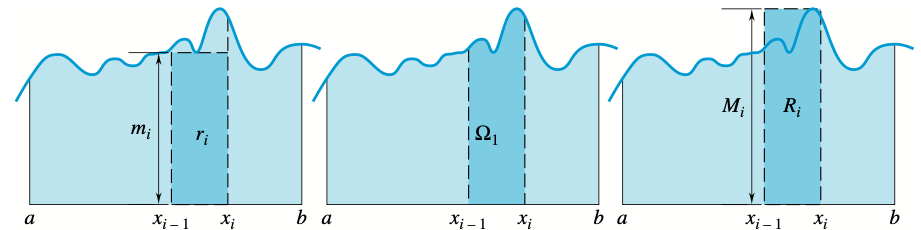
\includegraphics[width=.9\textwidth]{pics/area-omega-i.png}
}

Dado que el área de un rectángulo es el producto de la base por la altura, obtenemos
\[
m_i\, (x_i-x_i-1)
\le \area(\Omega_i) \le
M_i\, (x_i-x_i-1),
\qquad\text{para $i=1,2,\dots,n$}.
\]
Definiendo $\Delta x_i=x_i-x_{i-1}$ tenemos que 
\[
m_i\, \Delta x_i
\le \area(\Omega_i) \le
M_i\, \Delta x_i,
\qquad\text{para $i=1,2,\dots,n$}.
\]
Sumando, obtenemos
\begin{equation}
  \label{eq:L<I<U}
m_1 \Delta x_1 + m_2 \Delta x_2 + \dots + m_n \Delta x_N
\le \area(\Omega) \le
M_1 \Delta x_1 + M_2 \Delta x_2 + \dots + M_n \Delta x_N.
\end{equation}
La suma $m_1 \Delta x_1 + m_2 \Delta x_2 + \dots + m_n \Delta x_N$ es una \emph{suma inferior de $f$} 
y la suma $M_1 \Delta x_1 + M_2 \Delta x_2 + \dots + M_n \Delta x_N$ es una \emph{suma superior de $f$}.

\centerline{
  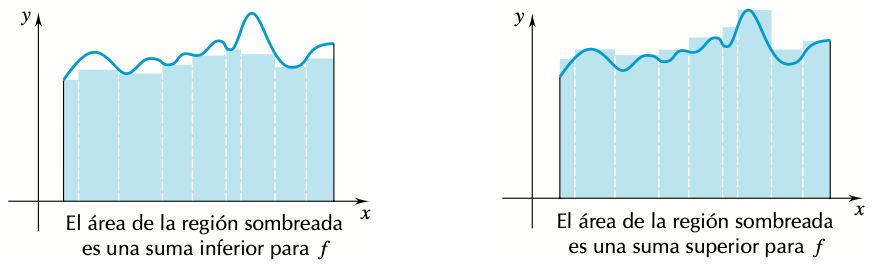
\includegraphics[width=.9\textwidth]{pics/sumas-superiores-inferiores.png}
}

La desigualdad~\eqref{eq:L<I<U} nos dice que para que un número pueda ser candidato al título de \emph{área de $\Omega$}, tal número ha de ser mayor o igual que cualquier suma inferior de $f$ y menor o igual que cualquier suma superior de $f$. Puede demostrarse, aunque no lo veremos aquí, que si $f$ es una función continua en $[a,b]$ entonces existe un número y sólo uno que cumple estas condiciones. A tal número lo llamaremos \emph{área de $\Omega$}.

\subsection*{Integral definida}

El procedimiento seguido para resolver el problema de área se llama \emph{integración} y el resultado final de este procedimiento se denomina \emph{integral definida}. A continuación estableceremos estas nociones con más precisión.

\begin{definition}
  Llamaremos \emph{partición} del intervalo cerrado $[a,b]$ a todo subconjunto finito de $[a,b]$ que contenga a los extremos. Es conveniente identificar los elementos de la partición con un índice acorde al orden narural. Así, cuando escribimos que 
  \[
  P=\{x_0,x_1, \dots ,x_n\} \text{ es una partición de $[a,b]$},
  \]
  entendemos que $\D a=x_0<x_1<\dots<x_n=b$.
\end{definition}

Supongamos ahora que $f$ es una función continua sobre $[a,b]$. En cada subintervalo $[x_{i-1},x_i]$ la función $f$ toma entonces un valor máximo $M_i$ y un mínimo $m_i$. Definimos entonces:

\begin{definition}
  Sea $f$ una función continua sobre $[a,b]$ y sea $P=\{a=x_0<x_1<\dots<x_n=b\}$ una partición de $[a,b]$. Luego definimos, para cada $i=1,2,\dots,n$:
  \[ 
    m_i = \min_{[x_{i-1},x_i]}f,
    \qquad
    M_i = \max_{[x_{i-1},x_i]}f.
  \]
  El número 
  \[
  L(P,f)= m_1 \Delta x_1 + m_2 \Delta x_2 + \dots + m_n \Delta x_N 
  = \sum_{i=1}^n m_i \Delta x_i,
  \]
  se denomina
  \emph{suma inferior de $f$ correspondiente a la partición $P$};
  y el número 
  \[
  U(P,f)= M_1 \Delta x_1 + M_2 \Delta x_2 + \dots + M_n \Delta x_N
  = \sum_{i=1}^n M_i \Delta x_i,
  \]
  se denomina \emph{suma superior de $f$ correspondiente a la partición $P$}.
\end{definition}

\begin{theorem}
  Si $f$ es una función continua en $[a,b]$ existe un único número $I$ que satisface la desigualdad 
  \[
  L(P,f)\le I\le U(P,f),
  \qquad\text{para toda partición $P$ de $[a,b]$}
  \]
\end{theorem}

\begin{proof}
  La demostración de este teorema queda fuera del alcance de este apunte, y será discutida en las clases de Coloquio de Demostraciones.
\end{proof}

A partir de este último teorema llegamos a la definición principal de esta sección:

\begin{definition}[Integral definida]
  Sea $f$ una función continua en $[a,b]$. El único número $I$ que satisface 
  \[
    L(P,f)\le I\le U(P,f),
    \qquad\text{para toda partición $P$ de $[a,b]$}
  \]
  se llama \emph{integral definida} (o simplemente \emph{integral}) de $f$ entre $a$ y $b$ y se designa por
  \[
  \int_a^b f(x)\dx.
  \]
\end{definition}

El símbolo $\int$ fue introducido por Leibniz y se llama \emph{signo integral}. En realidad es una \emph{S} (de \emph{suma}) estirada. Los números $a$ y $b$ se denominan \emph{límites de integración} ($a$ es el límite inferior y $b$ el límite superior). La función a integrar se llama \emph{integrando}. En algunos libros suele escribirse más brevemente $\int_a^b f$, omitiendo la variable $x$.

En la expresión $\int_a^b f(x)\dx$ la variable $x$ es una \emph{variable muda}. Esto quiere decir que puede ser sustituida por cualquier otra letra no utilizada hasta el momento. Así:
\[
\int_a^b f(x)\, dx
= \int_a^b f(t)\, dt
= \int_a^b f(u)\, du
= \int_a^b f(z)\, dz.
\]

En la introducción a este capítulo comenzamos con una aplicación inmediata de la integral definida:
Si $f$ es no negativa en $[a,b]$, entonces
\[
A = \int_a^b f(x)\dx
\]
da como resultado el área debajo de la gráfica de $f$.
Volveremos más adelante sobre esta aplicación.
Ahora veamos algunos ejemplos sencillos que nos ayudarán a comprender la definición.

\begin{example}
  Si $f(x)=c$, una constante, para todo $x\in[a,b]$, ?`cuánto vale $\int_a^b f(x)\dx$?

  Veamos, si $P=\{a=x_0<x_1<\dots<x_n=b\}$ es una partición de $[a,b]$, tenemos que 
\[ 
    m_i = \min_{[x_{i-1},x_i]}f = c
    \qquad
    M_i = \max_{[x_{i-1},x_i]}f = c;
  \]
  por lo que 
  \[
  L(P,f)
  = \sum_{i=1}^n m_i \Delta x_i
  = \sum_{i=1}^n c \Delta x_i
  = c \sum_{i=1}^n \Delta x_i
  = c (b-a)
  \]
  y 
  \[
  U(P,f)
  = \sum_{i=1}^n M_i \Delta x_i
  = \sum_{i=1}^n c \Delta x_i
  = c \sum_{i=1}^n \Delta x_i
  = c (b-a).
  \]
  Luego, 
  \[
    L(P,f)\le c(b-a)\le U(P,f),
    \qquad\text{para toda partición $P$ de $[a,b]$},
  \]
  y concluimos que 
  \[
  \int_a^b f(x)\dx = \int_a^b c \dx = c (b-a).
  \]

  Como ejemplos concretos:
  \begin{align*}
    \int_{-1}^1 3 \dx = 3 \big(1 - (-1)\big) = 3 \cdot 2 = 6;
    % \qquad\text{y}
    \\
    \int_{4}^{10} -3 \dx = -2 \big(10 - 4\big) = -2 \cdot 6 = -12.
  \end{align*}
\end{example}

\begin{example}
  Nos proponemos estudiar ahora la integral de la función $f(x)=x$, es decir $\int_a^b x\dx$.
  Veamos, si $P=\{a=x_0<x_1<\dots<x_n=b\}$ es una partición de $[a,b]$, tenemos que 
  \[ 
      m_i = \min_{[x_{i-1},x_i]}f = x_{i-1}
      \qquad
      M_i = \max_{[x_{i-1},x_i]}f = x_i;
    \]
    por lo que 
    \[
    L(P,f)
    = \sum_{i=1}^n m_i \Delta x_i
    = \sum_{i=1}^n x_{i-1} (x_{i}-x_{i-1})
    \]
    y 
    \[
    U(P,f)
    = \sum_{i=1}^n M_i \Delta x_i
    = \sum_{i=1}^n x_{i} (x_{i}-x_{i-1}).
    \]
    Observamos que para cada índice $i=1,2,\dots,n$, 
    \[
    x_{i-1}\le \frac12 (x_i+x_{i-1})\le x_i.
    \]
    Luego, multiplicando por $\Delta x_i = x_i-x_{i-1}>0$, tenemos que
    \[
    x_{i-1} \Delta x_i 
    \le \frac12 (x_i+x_{i-1})(x_i-x_{i-1}) 
    = \frac12 (x_i^2-x_{i-1}^2) = 
    \le x_i \Delta x_i.
    \]
    Sumando para $i$ de $1$ a $n$ obtenemos
    \[
    L(P,f) \le \sum_{i=1}^n \frac12 (x_i^2-x_{i-1}^2) \le U(P,f).
    \]
    Pero 
    \begin{align*}
      \sum_{i=1}^n \frac12 (x_i^2-x_{i-1}^2)
      &= \frac12 \Big[ (x_1^2-x_0^2) + (x_2^2-x_1^2) + \dots + (x_n^2-x_{n-1}^2)  \Big]
      \\
      &= \frac12 \big(x_n^2-x_0^2\big)
      = \frac12 \big(b^2-a^2\big).
    \end{align*}
    Luego, 
    \[
      L(P,f)\le \frac12 \big(b^2-a^2\big) \le U(P,f),
      \qquad\text{para toda partición $P$ de $[a,b]$},
    \]
    y por lo tanto
    \[
    \int_a^b x\dx = \frac12 \big(b^2-a^2\big).
    \]
    Como ejemplos concretos:
    \begin{align*}
      \int_{-1}^1 x \dx = \frac12 \big(3^2 - (-1)^2\big) = \frac12 \cdot 8 = 4;
      % \qquad\text{y}
      \\
      \int_{-2}^{2} x \dx = \frac12 \big(2^2 - (-2)^2\big) = \frac12 \cdot 0 = 0.
    \end{align*}\end{example}

\begin{example}
  Consideremos un último ejemplo, de una función \emph{discontinua}, pero \emph{continua a trozos}.
  Sea 
  \[
  f(x)=\begin{cases}
    0, \quad&\text{si $x\neq 1$},
    \\
    1, \quad&\text{si $x=1$}.
  \end{cases}
  \]
  Afirmamos que $\int_0^2 f(x)\dx=0$, es decir, cambiar el valor de la función en un punto no afecta el valor de la integral.
  Claramente, cualquiera sea la partición $P$ del intervalo $[0,2]$, se tiene que 
  \[
  0=L(P,f) \le 0 \le U(P,f).
  \]
  Veamos que $0$ es el único número que cumple dicha desigualdad para toda partición.
  Consideremos la partición $P_\epsilon = \{0, 1-\epsilon, 1+\epsilon, 2\}$, para $0<\epsilon<1$.
  Luego, $L(P_\epsilon,f)=0$ y 
  \[
  U(P,f)=0 (x_1-x_0) + 1 (x_2-x_1) + 0 (x_3-x_2)
  = (x_2-x_1)= \big((1+\epsilon)-(1-\epsilon)\big)=2\epsilon.
  \]
  El único número que cumple $0\le I \le 2\epsilon$ para todo $\epsilon\in(0,1)$ es $I=0$.
  Por lo tanto $\int_0^2 f(x)\dx=0$.
\end{example}


\subsubsection*{Ejercicios de la sección~\getcurrentref{chapter}.\getcurrentref{section}}

\begin{enumerate}
\item Hallar $L(P,f)$ y $U(P,f)$ en cada uno de los siguientes casos:
\begin{enumerate}
  \item $\D f(x) = 1-x$, $P=\{0, \frac13, \frac34, 1, 2\}$
  \item $\D f(x) = \sqrt{x}$, $P=\{0, \frac1{25}, \frac4{25}, \frac9{25}, \frac{16}{25}, 1\}$
  \item $\D f(x) = x^2$, $P=\{-1,-\frac12, -\frac14, 0, \frac14, \frac12, 1\}$
\end{enumerate}

\item Sea $f$ una función continua en $[-1,1]$. Explicar por qué cada una de las siguientes afirmaciones es falsa.
\begin{enumerate}
  \item $L(P,f)=3$ y $U(P,f)=2$.
  \item $L(P,f)=3$ y $U(P,f)=6$ y $\int_{-1}^1 f(x)\dx=2$.
  \item $L(P,f)=3$ y $U(P,f)=6$ y $\int_{-1}^1 f(x)\dx=10$.
\end{enumerate}

\item Sea $f:[0,1]\to \R$ definida por
\[
\begin{cases}
  1, \quad&\text{si $x\in\Q$,}
 \\ 
 0, \quad&\text{si $x\notin\Q$.}
\end{cases}
\]
Si $P$ es una partición de $[0,1]$.
?`Cuánto valen $L(P,f)$ y $U(P,f)$?
?`Cuántos números $I$ hay que cumplen $L(P,f) \le I \le U(P,f)$, para toda partición $P$?
\end{enumerate}


\section{El Teorema Fundamental del Cálculo}
  %La función \texorpdfstring{$F(x)=\int_a^x f(t)\dx$}{integral hasta \emph{x}}}

En los ejemplos de la sección anterior tuvimos que confiar en que se nos ocurriera una idea para saber cómo encontrar el número $I$ que da la integral. En esta sección estudiaremos propiedades de la integral que nos permitirán encontrar una forma más sistemática y sencilla de calcular integrales.

Para ello necesitamos primero la siguiente Proposición.

\begin{proposition}
  Sea $f$ es continua en $[a,b]$, y sean $P$ y $Q$ dos particiones del intervalo $[a,b]$.
  Si $P\subset Q$, entonces 
  \[
  L(P,f) \le L(Q,f)
  \qquad\text{y}\qquad
  U(Q,f) \le U(P,f).
  \]
  Es decir, al agregar puntos a una partición, \emph{las sumas inferiores crecen} y \emph{las sumas superiores decrecen}.
\end{proposition}

\begin{proof}
  Basta con probar el caso en que $Q$ tiene un punto más que $P$, luego proceder por inducción.
  Supongamos entonces que $P=\{a=x_0<x_2<\dots<x_n=b\}$ y que $Q = P\cup \{p\}$. Sea $i_0\in\{x_1,x_2,\dots,x_n\}$ tal que $x_{i_0-1}<p<x_{i_0}$.
  Gráficamente, la situación en ese intervalo se vería así:

  \centerline{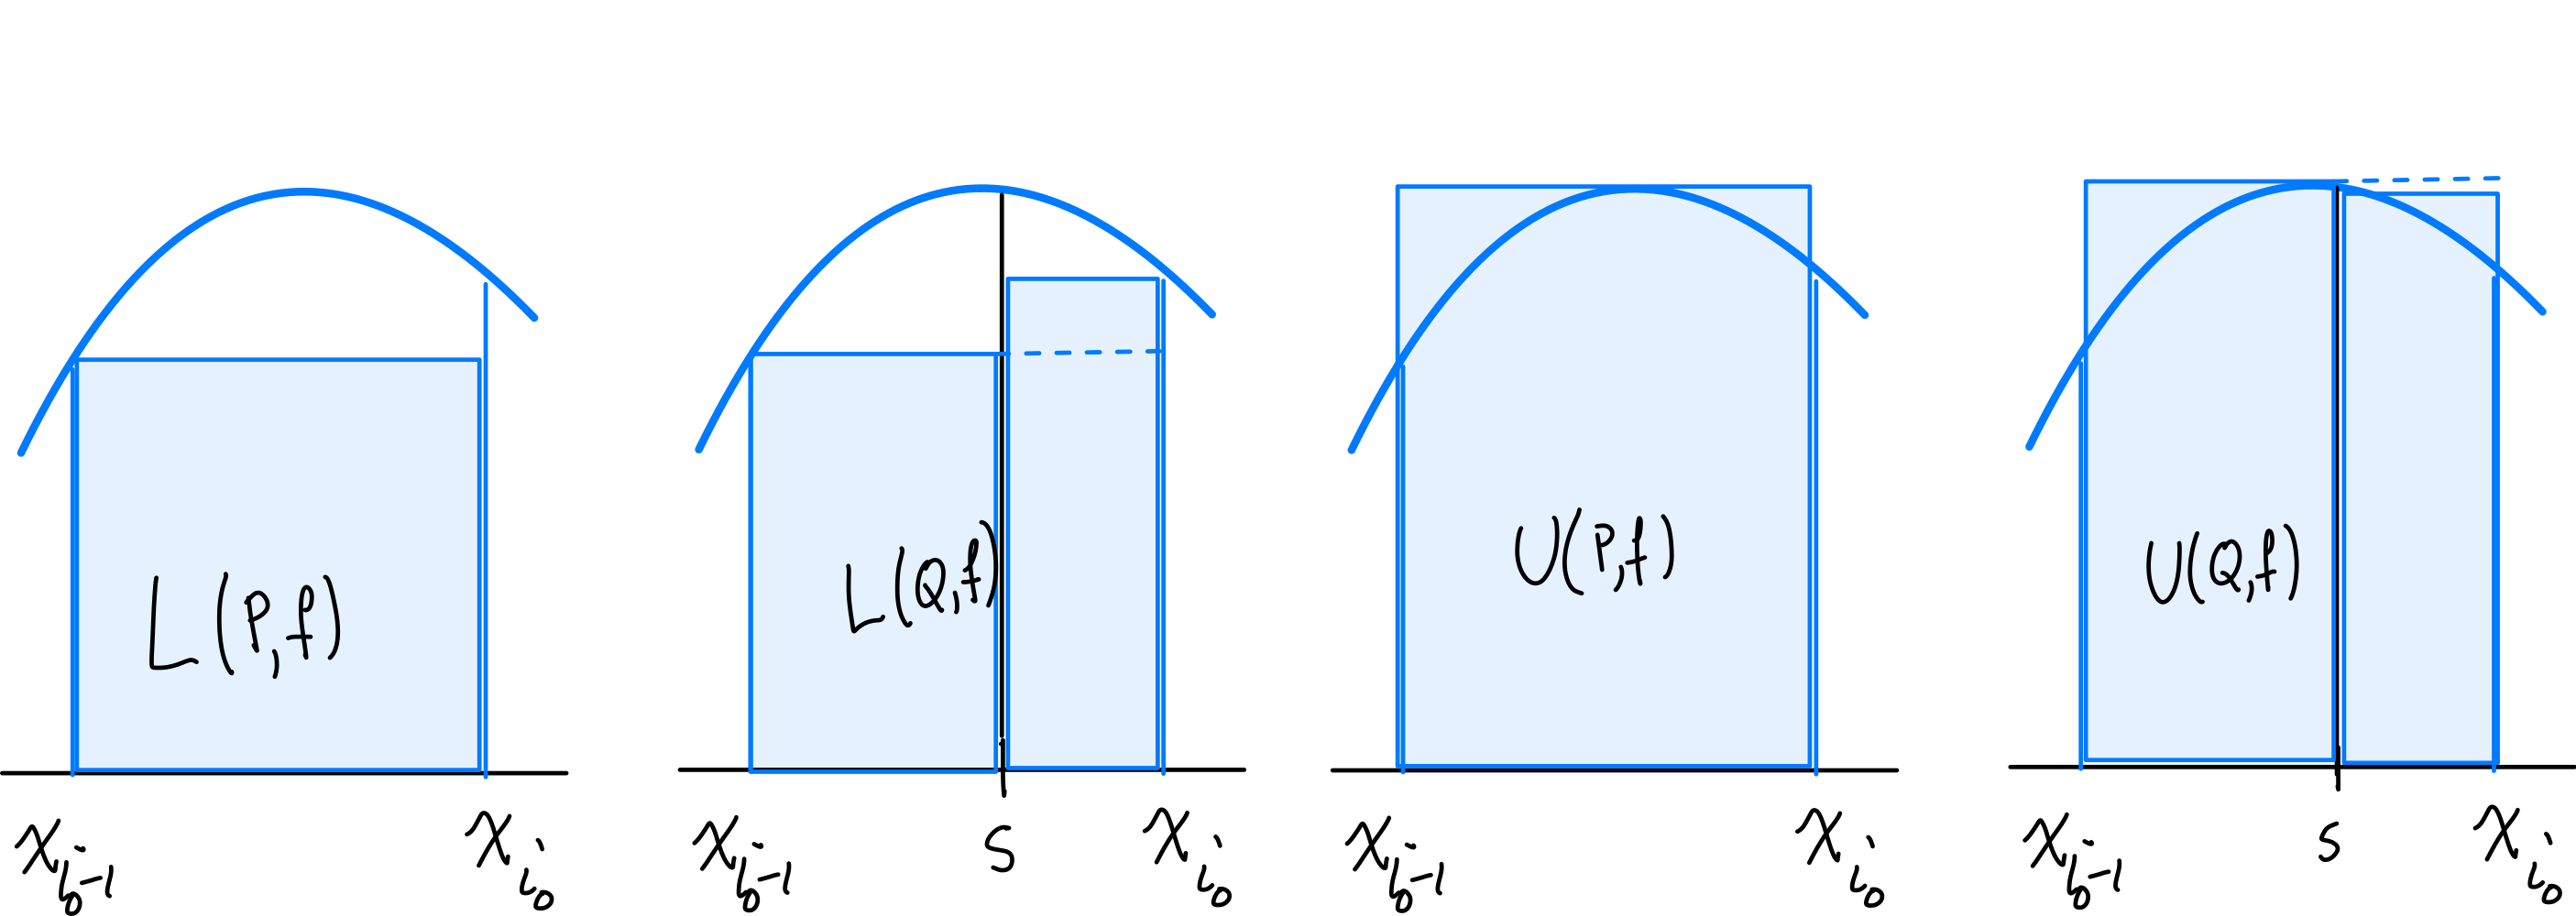
\includegraphics[width=.8\textwidth]{pics/sumas-insertar-punto.png}}

  Por lo tanto, el único término de la suma inferior de $P$ que se cambia, cambia por dos términos que al sumarlos dan mayor o igual al término original.
  Y el único término de la suma superior de $P$ que se cambia, cambia por dos términos que al sumarlos dan menor o igual al término original. 
  De aquí concluimos la afirmación de la proposición.
\end{proof}

El siguiente teorema es bastante obvio si pensamos en la interpretación geométrica de la integral como un área.

\begin{theorem}
  Si $f$ es continua en $[a,b]$ y $a<c<b$, entonces
  \[
  \int_a^b f(x)\dx = \int_a^c f(x)\dx + \int_c^b f(x)\dx.
  \]
\end{theorem}

\noindent
\begin{minipage}{.6\textwidth}
  \[ \area(I)+\area(II)=\area(\text{región completa})\]
\end{minipage}
\begin{minipage}{.39\textwidth}
\centerline{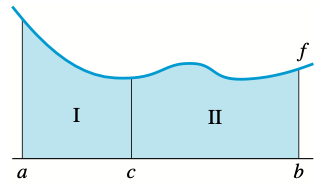
\includegraphics[width=.8\textwidth]{pics/integral-suma-intervalos.png}}
\end{minipage}

\begin{proof}
  Para demostrar el teorema basta con que demostremos que para toda partición $P$ de $[a,b]$ se verifica que
  \[
  L(P,f) \le \int_a^c f(x)\dx + \int_c^b f(x)\dx \le U(P,f).
  \]
  Consideremos entonces una partición arbitraria $P$ de $[a,b]$ y sea $Q=P\cup\{c\}\supset P$.
  Por la proposición anterior 
  \[
  L(P,f) \le L(Q,f)
  \qquad\text{y}\qquad
  U(Q,f) \le U(P,f).
  \]
  Ahora consideramos subparticiones de $Q$ en los intervalos $[a,c]$ y $[c,b]$:
  \[
  Q_1 = Q\cap[a,c]\qquad\text y\qquad 
  Q_2 = Q\cap[c,b].
  \]
  Luego $Q_1$ y $Q_2$ son particiones de $[a,c]$ y de $[c,b]$ respectivamente, por lo tanto:
  \[
  L(Q_1,f)\le \int_a^c f(x)\dx \le U(Q_1,f)
  \qquad\text{y}\qquad
  L(Q_2,f)\le \int_c^b f(x)\dx \le U(Q_2,f).
  \]
  Sumando estas desigualdades obtenemos
  \[
  L(Q_1,f)+L(Q_2,f)\le \int_a^c f(x)\dx + \int_c^b f(x)\dx \le U(Q_1,f)+U(Q_2,f).
  \]
  Finalmente observamos que 
  \[
    L(Q_1,f)+L(Q_2,f) = L(Q,f)
    \qquad\text y\qquad
    U(Q_1,f)+U(Q_2,f) = U(Q,f),
  \]
  que implica lo que queríamos demostrar.
  \end{proof}

  \begin{definition}
    A partir de este último teorema, hacemos las siguientes definiciones, que de alguna manera generalizan la definición de integral.
    \begin{enumerate}
      \item Si $f:[a,b]\to \R$ tiene una discontinuidad de salto en $c\in (a,b)$ pero es continua en $(a,c)$ y en $(c,b)$, entonces
      \[
      \int_a^b f(x)\dx = \int_a^c f(x)\dx + \int_c^b f(x)\dx.
      \]
      \item Hasta ahora sólo hemos definido integrales \emph{de izquierda a derecha}: desde un número $a$ hasta un número $b$, con $b>a$. También puede integrarse en sentido opuesto, a través de la siguiente definición:
      \[
      \int_b^a f(x)\dx 
      = -\int_a^b f(x)\dx .
      \]
      \item Además, la integral cuando los extremos de integración coinciden se define como cero:
      \[
      \int_c^c f(x)\dx = 0.
      \]
        \end{enumerate}
  \end{definition}

  \begin{remark}
    A partir de las últimas definiciones, observamos que la siguiente igualdad
      \[
        \int_a^c f(x)\dx + \int_c^b f(x)\dx=\int_a^b f(x)\dx ,
      \]
    se cumple independientemente del orden en que se encuentren $a$, $b$ y $c$.
  \end{remark}

\noindent
\begin{minipage}{.4\textwidth}  Dada una función continua $f$, definimos 
  \[
  F(x)=\int_a^x f(t)\dt.
  \]
  Es decir, $F(x)$ es el área de la región sombreada en las figuras, que varía al variar $x$.
\end{minipage}
\begin{minipage}{.6\textwidth}
  \begin{center}
    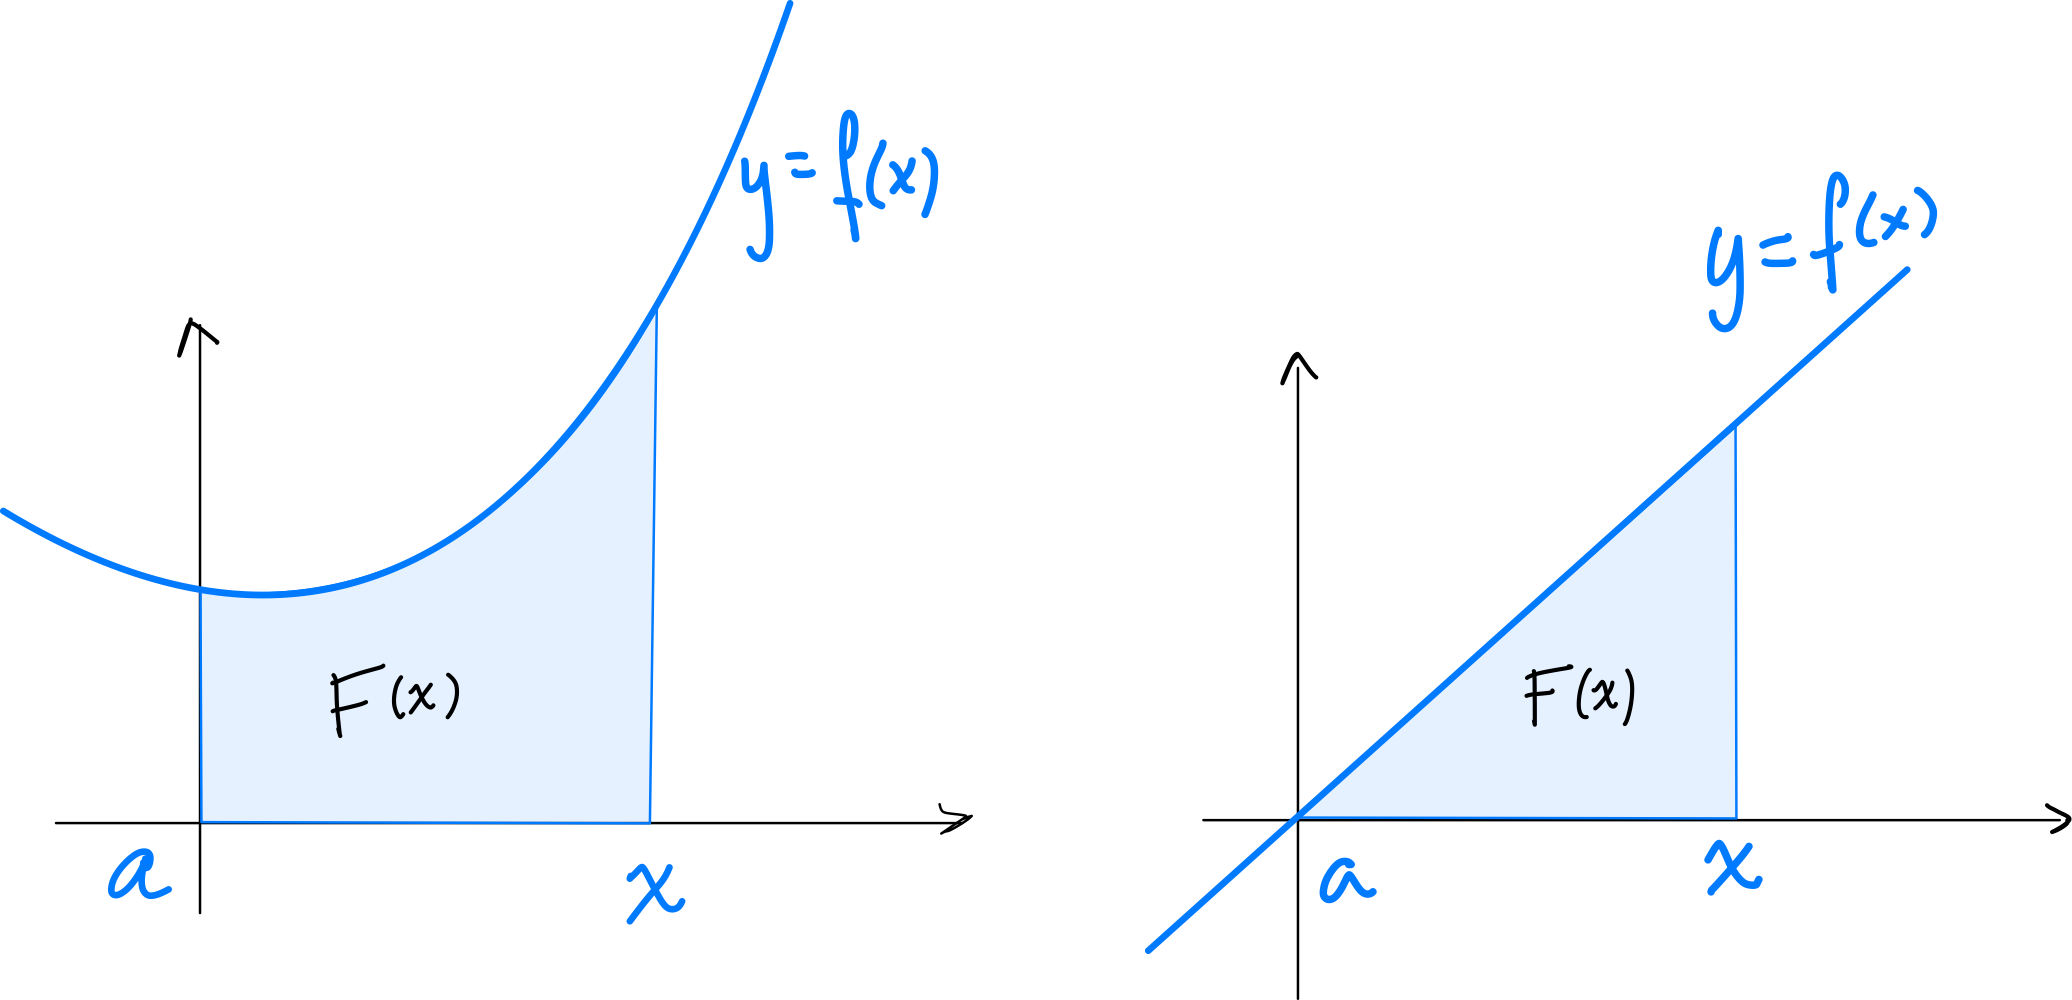
\includegraphics[width=.95\textwidth]{pics/integral-hasta-x.png}
  \end{center}
\end{minipage}

El siguiente teorema se conoce como Teorema Fundamental del Cálculo, y relaciona el concepto nuevo de integral con el de derivada, de la siguiente manera:

\begin{theorem}\label{T:TFC}
  Si $f$ es continua en $[a,b]$ y definimos $F:[a,b]\to\R$ como 
  \[
  F(x)=\int_a^x f(t)\dt,
  \]
  Entonces $F$ es continua en $[a,b]$ y diferenciable en $(a,b)$ y más aún, 
  \[
  F'(x)=f(x),\quad\text{para todo $x\in(a,b)$.}
  \]
\end{theorem}

\begin{proof}
  Comenzamos considerando $x\in[a,b)$ y veremos que 
  \[\lim_{h\to 0^+}\frac{F(x+h)-F(x)}{h}=f(x).\]
  Si $x<x+h\le b$, entonces
  \[F(x+h)-F(x)=\int_a^{x+h}f(t)\dt - \int_a^x f(t)\dt = \int_x^{x+h}f(t)\dt.\]
  Definimos ahora 
  $$ M_h = \max_{[x,x+h]}f\qquad\text y\qquad
  m_h = \min_{[x,x+h]}f.$$
  Entonces, 
  $$ M_h \cdot \big( (x+h)-x \big) = M_h \cdot h $$
  es una suma superior para $f$ en $[x,x+h]$ y
  $$ m_h \cdot \big( (x+h)-x \big) = m_h \cdot h $$ 
  es una suma inferior para $f$ en $[x,x+h]$.
  Luego
  $$ m_h \cdot h \le \int_x^{x+h}f(t)\dt \le M_h\cdot h,$$
  que a su vez implica
  $$ m_h \le \frac{\int_x^{x+h}f(t)\dt}h \le M_h.$$
  Es decir,
  $$ m_h \le \frac{F(x+h)-F(x)}h \le M_h.$$
  Como $f$ es continua en $[a,b]$
  \[
  \lim_{h\to0^+} m_h = f(x) = \lim_{h\to 0^+} M_h,
  \]
  y por el teorema del emparedado
  \begin{equation}\label{eq:TFC-der}
    \lim_{h\to 0^+} \frac{F(x+h)-F(x)}h = f(x).
  \end{equation}

  De manera análoga se puede demostrar que, para $x\in(a,b]$ se verifica
  \begin{equation}\label{eq:TFC-izq}
    \lim_{h\to 0^-} \frac{F(x+h)-F(x)}h = f(x).
  \end{equation}
  Esto implica que para $x\in(a,b)$ se cumplen~\eqref{eq:TFC-der} y~\eqref{eq:TFC-der} a la vez, 
  \[
  F'(x)= \lim_{h\to 0} \frac{F(x+h)-F(x)}h = f(x).
  \]
  Esto muestra que $F(x)$ es diferenciable en $(a,b)$ y su derivada es $F'(x)=f(x)$.

  Solo queda probar que $F$ es continua por derecha en $a$ y continua por izquierda en $b$.
  A partir de~\eqref{eq:TFC-der} en $a$ obtenemos
  $$ 
  \lim_{h\to 0^+} \frac{F(a+h)-F(a)}h = f(a),
  $$ 
  Que a su vez implica que
  $$ 
  \lim_{h\to 0^+} \big(F(a+h)-F(a)\big)
  = \lim_{h\to 0^+}\Big( h\cdot \frac{F(a+h)-F(a)}h \Big)= f(a)\cdot 0 = 0.
  $$ 
  Por lo tanto $\lim_{h\to 0^+} F(a+h)=F(a)$ y $F$ es continua por derecha en $a$.
  Análogamente se puede demostrar que $F$ es continua por izquierda en $b$, usando~\eqref{eq:TFC-izq}.
\end{proof}

\begin{example}
  Si $F$ está definida por 
  \[
  F(x)=\int_{-1}^x (2t+t^2) \dt,
  \qquad \text{para $-1\le x\le 5$},
  \]
  Entonces $F'(x) = 2x+x^2$.
\end{example}


\begin{example}
  Si $F$ está definida por 
  \[
  F(x)=\int_{0}^x \sen(\pi t) \dt,
  \qquad \text{para $x\in\R$},
  \]
  Entonces $F'(x) = \sen(\pi x)$.
\end{example}

A continuación veremos cómo este teorema nos sirve para calcular integrales definidas de un gran número de funciones. Para ello hacemos primero la siguiente definición.

\begin{definition}[Antiderivada]
  Sea $f$ una función continua en $[a,b]$. Una función $G$ se llama \emph{antiderivada} de $f$ en $[a,b]$ si y sólo si
  \[
  G\text{ es continua en $[a,b]$ \quad y \quad}
  G'(x)=f(x) \text{ para todo $x\in(a,b)$.}\]
\end{definition}

El Teorema~\ref{T:TFC} nos dice que, si $f$ es continua en $[a,b]$, entonces la función $F(x)$ definida por 
\[
  F(x)=\int_a^x f(t)\dt.
\]
es una antiderivada de $f$.
A partir del \emph{Teorema Fundamental del Cálculo} llegamos a un método que nos permite calcular integrales. Podemos calcular $\D\int_a^b f(t)\dt$ hallando una antiderivada de $f$.

\begin{theorem}[Regla de Barrow]
  Sea $f$ una función continua en $[a,b]$. Si $G$ es una antiderivada de $f$ en $[a,b]$, entonces
  $$ \int_a^b f(t)\dt = G(b)-G(a). $$
\end{theorem}

\begin{proof}
  Consideremos la función $F:[a,b]\to \R$ definida por $\D  F(x)=\int_a^x f(t)\dt$. 
  Luego, por un lado, 
  $$F(a)=\int_a^a f(t)\dt = 0,\qquad\text y\qquad  F(b)=\int_a^b f(t)\dt.$$

  Por otro lado, por el Teorema~\ref{T:TFC},
  $F(x)$ es una antiderivada de $f$, al igual que $G$. Luego,
  \[
  F'(x)=f(x)\quad\text y\quad G'(x)=f(x),\qquad\text{para todo $x\in(a,b)$.}
  \]
  Por el Corolario~\ref{C:f=g+k}, resulta que existe una constante $k\in\R$ tal que 
  \[
  F(x) = G(x) + k,
  \qquad\text{para todo $x\in[a,b]$.}
  \]
  Como $F(a)=0$, resulta que $G(a)+k=0$, es decir, $k = -G(a)$.
  Por lo tanto
  \[
  F(x) = G(x) - G(a),
  \qquad\text{para todo $x\in[a,b]$.}
  \]
  En particular, 
  \[
  F(b) = \int_a^b f(t)\dt = G(b)-G(a),
  \]
  que es lo que se quería demostrar.
\end{proof}

De este último teorema, obtenemos un procedimiento para calcular integrales.
\begin{quote}
  Para calcular $\D\int_a^b f(t)\dt$, debemos hacer lo siguiente:
  \begin{enumerate}
    \item Hallar una antiderivada $G$ de $f$.
    \item Calcular $G(b)-G(a)$. Ese resultado es $\D\int_a^b f(t)\dt$.
    \item FIN.
  \end{enumerate}
\end{quote}


\begin{example}
  Calcular $\D \int_1^4 x^2 \dx$.

  Debemos hallar una antiderivada de $f(x)=x^2$. Inspeccionando la tabla de derivadas, vemos que $\dd[]{x^3}{x} = 3 \,x^2$. Luego, $\D\dd{}{x}\frac{x^3}3 = x^2$ y por lo tanto $G(x)=\D\frac{x^3}3 $ es una antiderivada de $f(x)=x^2$. Luego, aplicando el teorema fundamental del Cálculo,
  \[
    \int_1^4 x^2 \dx = G(4) - G(1) = \frac{4^3}3-\frac{1^3}3 = \frac{64}3-\frac13=21.
  \]
\end{example}

\begin{example}
  Consideremos ahora el cálculo de $\D\int_0^{\pi/2} \sen x \dx$.

  Tenemos que hallar una antiderivada de $\sen x$.
  Inspeccionando nuestra memoria, recordamos que $\dd{\cos x}{x}=-\sen x$, luego $-\cos x$ es una antiderivada de $\sen x$. Entonces
  \[
  \int_0^{\pi/2} \sen x\dx = (-\cos \frac\pi2)-(-\cos 0)=0-(-1)=1.
  \]
\end{example}

Resulta un poco trabajoso escribir todo ese texto sobre la antiderivada, para eso viene bien la notación siguiente:
\[
\big[G(x)\big]_a^b = G(b)-G(a).
\]
Así, el cálculo de las integrales de los ejemplos anteriores se puede escribir en una sola línea, dejando en claro los pasos, de la siguiente manera:
\begin{align*}
  \int_1^4 x^2 \dx &= \Big[ \frac{x^3}{3}\Big]_1^4 =\frac{4^3}3-\frac{1^3}3 = \frac{64}3-\frac13=21,
  \\
  \int_0^{\pi/2} \sen x\dx &= \Big[ -\cos x \Big]_{0}^{\pi/2} = (-\cos \frac\pi2)-(-\cos 0)=0-(-1)=1.
\end{align*}

En general, el cálculo de antiderivadas no es tan sencillo como el de derivadas, pero con lo que sabemos, y la observación que sigue, podemos calcular antiderivadas de una gran familia de funciones:

\begin{remark}
  Si $F$ y $G$ son antiderivadas de $f$ y $g$ respectivamente, entonces una antiderivada de $c\, f(x)+d\, g(x)$ es 
  $c\, F(x) + d\, G(x)$, cualesquiera sean las constantes $c$ y $d$.
  En efecto, como la derivada es lineal
  $$ 
  \dd[]{}{x}\big[c\, F(x) + d\, G(x) \big] = c\, F'(x)+d\,G'(x) = c\, f(x)+d\, g(x).
  $$
\end{remark}

Esto implica que la integral es lineal.

\begin{corollary}[Linealidad de la integral]
Si $f$ y $g$ son funciones continuas en $[a,b]$ y $c$ y $d$ son dos constantes, entonces
$$ 
\int_a^b   c\, f(x)+d\, g(x) \dx 
=
c\, \int_a^b  f(x) \dx 
+
d\, \int_a^b   g(x) \dx .
$$
\end{corollary}

\begin{proof}
  Sean $F$ y $G$ antiderivadas de $f$ y $g$, respectivamente.
  Por el comentario previo, $c\, F(x) + d\, G(x)$ es una antiderivada de $c\, f(x)+d\, g(x)$.
  Luego
  \begin{align*}
    \int_a^b   c\, f(x)+d\, g(x) \dx  &= \Big[c\, F(x) + d\, G(x)\Big]_a^b
    \\
    &= \big[c\, F(b) + d\, G(b)\big] - \big[c\, F(a) + d\, G(a)\big]
    \\
    &= c \big[F(b)-F(a)\big] + d \big[G(b)-G(a)\big] 
    \\
    &= c\, \int_a^b  f(x) \dx 
    +
    d\, \int_a^b   g(x) \dx .
    \qedhere
  \end{align*}
\end{proof}

\begin{example}
  Con este último resultado podemos calcular la integral de funciones un poco más complicadas:
  \begin{align*}
    \int_0^\pi 9x^2 - 2 \sen x\dx
    &= 9 \int_0^\pi x^2 \dx - 2 \int_0^\pi \sen x\dx
    \\
    &= 9 \Big[ \frac{x^3}3\Big]_0^\pi  - 2 \Big[-\cos x\Big]_0^\pi
    \\
    &= 9 \Big[ \frac{\pi^3}3-\frac{0^3}3\Big]  - 2 \Big[(-\cos \pi)-(-\cos 0)\Big]
    \\
    &= 9 \frac{\pi^3}3 - 2 \Big[(1)-(-1)\Big]
    = 3 \pi^3 - 4.
  \end{align*}
\end{example}

\begin{remark}
  !`Atención! Sólo \emph{las constantes} pueden sacarse fuera de la integral:
  \[
  \underbrace{\int_0^\pi x\, \sen x\dx}_{\text{número}} \neq \underbrace{x \  \overbrace{\int_0^\pi \sen x\dx}^{\text{número}}}_{\text{expresión variable}}.
  \]
  Para ver fácilmente que esto no es cierto, basta con observar que el lado izquierdo es un número y el lado derecho es una expresión variable, que aún depende de $x$.
\end{remark}



A continuación vemos un ejemplo más de cálculo de la derivada de una integral, cuando el extremo derecho no es $x$ sino una expresión que depende de $x$.


\begin{example}
  Calcular $\dd[]{}{x} \int_0^{x^2+1} \frac{\sen t}{t^4+t^2+1} \dt$.

  Aquí tenemos una composición de funciones. Si llamamos $\D f(y)=\int_0^{y} \frac{\sen t}{t^4+t^2+1} \dt$, y $g(x)=x^2+1$, entonces 
  \[
    \int_0^{x^2+1} \frac{\sen t}{t^4+t^2+1} \dt = f\circ g(x).
  \]
  Luego, por la regla de la cadena,
  \[
    \dd[]{}{x} \int_0^{x^2+1} \frac{\sen t}{t^4+t^2+1} \dt
    = (f\circ g)'(x) = f'(g(x))\, g'(x).
  \]
  Ahora sí, por el teorema fundamental del cálculo $f'(y)= \frac{\sen y}{y^4+y^2+1}$, y $g'(x)=2x$. Entonces
  \[
    \dd[]{}{x} \int_0^{x^2+1} \frac{\sen t}{t^4+t^2+1} \dt
    = \frac{\sen (x^2+1)}{(x^2+1)^4+(x^2+1)^2+1} \, 2\, x.
  \]
\end{example}

\subsubsection*{Ejercicios de la sección~\getcurrentref{chapter}.\getcurrentref{section}}

\begin{enumerate}
  \item Calcular las siguientes integrales
\begin{multicols}{2}
  \begin{enumerate}
    \item $\D \int_0^\pi \cos x \dx$.
    \item $\D \int_1^4 3 x^2 \dx$.
    \item $\D \int_1^e \frac1x \dx$.
    \item $\D \int_0^2 \big( x^2+3x+2\big) \dx$.
    \item $\D \int_0^1 \cosh x \dx$.
    \item $\D \int_1^4 \frac{1}{2\sqrt{x}} \dx$.
    \item $\D \int_4^9 \frac{1}{\sqrt x}\dx$.
    \item $\D \int_1^2 x^a \dx$, ($a\in \R$, $a\neq -1$).
  \end{enumerate}
\end{multicols}
\item Hallar el área de la región comprendida entre la gráfica de $f(x)$ y el eje de abscisas, para $x$ en el intervalo dado:
\begin{multicols}{2}
  \begin{enumerate}
    \item $\D f(x)=4x-x^2$; $[0,4]$.
    \item $\D f(x)=x\sqrt{x}+1$; $[1,9]$.
    \item $\D f(x)=2\cos x$; $[-\pi/2,\pi/4]$.
    \item $\D f(x)=\sen x$; $[0,\pi]$.
  \end{enumerate}
\end{multicols}

\item Hallar el área de la región comprendida entre la gráfica de $f(x)=\sen x$ y el eje de abscisas, para $x$ entre $0$ y $2\pi$.

\item Calcular las siguientes integrales
\begin{multicols}{2}
  \begin{enumerate}
    \item $\D \int_2^5 (x-3) \dx$.
    \item $\D \int_2^5 |x-3| \dx$.
    \item $\D \int_{-4}^2 (2x+3) \dx$.
    \item $\D \int_{-4}^2 |2x+3| \dx$.
  \end{enumerate}
\end{multicols}

\item Calcular la derivada de las siguientes funciones:
\begin{multicols}{2}
  \begin{enumerate}
    \item $\D \int_1^x (t+2)^2 \dt$.
    \item $\D \int_1^x (\cos t-\sen t)^2 \dt$.
    \item $\D \int_0^{2x+1} \frac{1}{1+t^2} \dt$.
    \item $\D \int_x^5 e^{-t^2} \dt$.
    \item $\D \int_{-x}^x e^{-t^2} \dt$.
    \item $\D \int_{-x^3}^{x^2+1} e^{-t^2} \dt$.
  \end{enumerate}
\end{multicols}

\item Calcular las siguientes integrales:
  \begin{enumerate}
    \item $\D \int_0^4 f(x)\dx$, con 
    $\D f(x)=\begin{cases}
      2x+1, \quad \text{si $0\le x \le 1$},
      \\
      4-x, \quad \text{si $1<x\le 4$}.
    \end{cases}
      $
      \item $\D \int_{-2}^4 f(x)\dx$, con 
          $\D f(x)=\begin{cases}
        x^2, \quad \text{si $-2\le x < 0$},
        \\
        \frac12 x+2, \quad \text{si $0\le x\le 4$}.
          \end{cases}
        $
  \end{enumerate}

\item Calcular la integral $\D\int_0^{5} \dd[]{(e^{-x^2})}{x}\dx$.

\item Si $f$ es una función diferenciable con $f'$ continua en $[a,b]$, ?`a qué es igual $\D\int_a^b f'(x) \dx$?
\end{enumerate}



\section{Algunos problemas de áreas}

Al comienzo de este capítulo vimos que si $f$ es no negativa y continua en $[a,b]$, entonces $\int_a^b f(x)\dx$ da el área de la región delimitada por la gráfica de  $f$, y el eje $x$ entre las rectas $x=a$ y $x=b$.

\noindent
\begin{minipage}{.7\textwidth}
$$ \area(\Omega)=\int_a^b f(x)\dx.$$
\end{minipage}
\begin{minipage}{.29\textwidth}
  \centering
  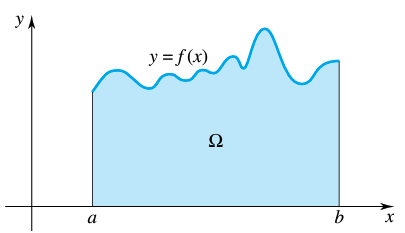
\includegraphics[width=.9\textwidth]{pics/area-bajo-curva.png}
\end{minipage}

\begin{example}
  Hallar el área debajo de la gráfica de la función raíz cuadrada entre $x=0$ y $x=1$.

  Como $\sqrt{x}\ge0$ para todo $x$, dicha área se calcula de la siguiente manera:
  \[
  \int_0^1 \sqrt{x}\dx = \int_0^1 x^{1/2}\dx 
  = \Big[ \frac{x^{1/2+1}}{1/2+1} \Big]_0^1
  = \Big[ \frac23x^{3/2} \Big]_0^1
  = \frac23 \cdot 1 - \frac23 \cdot 0 = \frac23.
  \]
\end{example}

\centerline{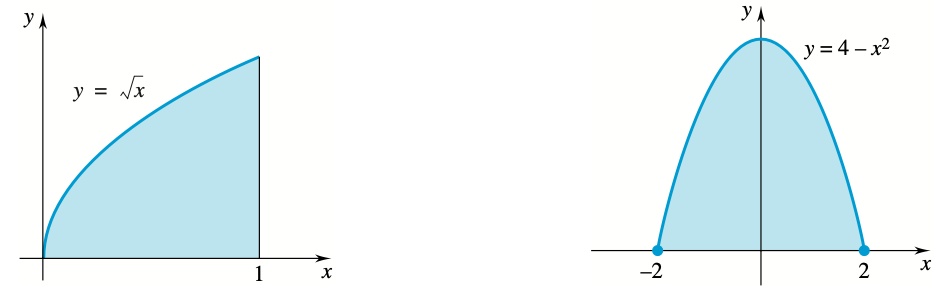
\includegraphics[width=.9\textwidth]{pics/areas-1.png}}

\begin{example}
  Hallar el área de la región comprendida entre la curva $y=4-x^2$ y el eje $x$.

  En este caso no nos dicen entre qué valores hay que tomar $x$. Entonces, tenemos que ver las intersecciones entre la curva $y=4-x^2$ y el eje $x$. Las intersecciones se encuentran en puntos con abscisas $x=-2$ y $x=2$ (ver figura).
  Luego calculamos el área integrando entre $-2$ y $2$:
  \[
  \int_{-2}^2 (4-x^2)\dx = \Big[ 4\, x-\frac13 x^3 \Big]_{-2}^2
  = \frac{32}3.
  \]
\end{example}

Consideremos ahora el área de la región $\Omega$ de la siguiente figura:

\centerline{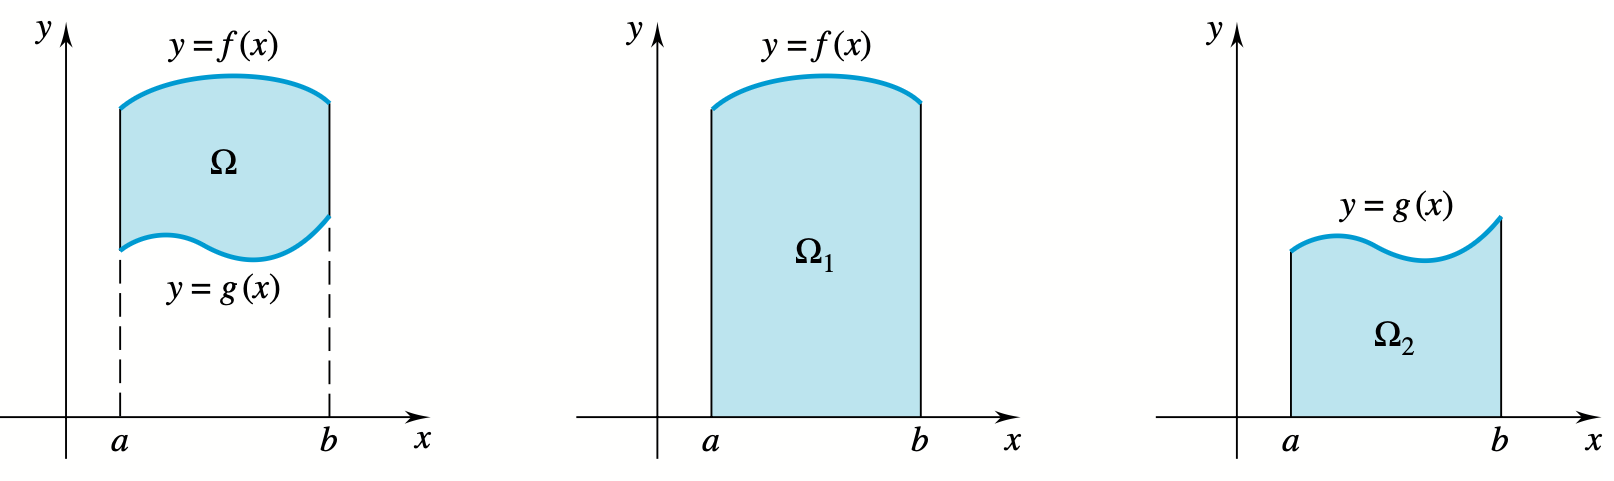
\includegraphics[width=.9\textwidth]{pics/areas-2.png}}

La frontera superior de $\Omega$ es la gráfica de la función no negativa $f$, y su frontera inferior es la gráfica de otra función no negativa $g$. Podemos obtener el área de $\Omega$ calculando el área de $\Omega_1$ y restándole el área de $\Omega_2$:
\begin{align*}
  \area(\Omega)&=\area(\Omega_1)-\area(\Omega_2)\\
  &= \int_a^b f(x)\dx - \int_a^b g(x)\dx.
\end{align*}
Por la linealidad de la integral, tenemos que
\begin{equation}\label{eq:area entre dos curvas}
  \area(\Omega) = \int_a^b \big[f(x)-g(x)\big]\dx.
\end{equation}

\begin{example}
  Hallemos el área de la región limitada por arriba por $y=x+2$ y por debajo por $y=x^2$.

  \noindent
  \begin{minipage}{.65\textwidth}
    El primer paso consiste en hallar los puntos de interseccipon de las dos curvas:
    \[
    x+2=x^2 \iff x^2-x-2=0 \iff x=-1 \text{ o } x=2.
    \]
    Por lo tanto las abscisas de los puntos de intersección son $x=-1$ y $x=-2$.
    Luego, el área de la región de interés es
    \begin{align*}
      \int_{-1}^2 \big[(x+2)-x^2\big]\dx 
      &= \Big[\frac{x^2}2+2x-\frac{x^3}3\Big]_{-1}^2
      \\ 
      &= \big[ 2 + 4 - \frac83\big]-\big[\frac12-2+\frac13\big]=\frac92.
    \end{align*}
  \end{minipage}
  \begin{minipage}{.34\textwidth}
    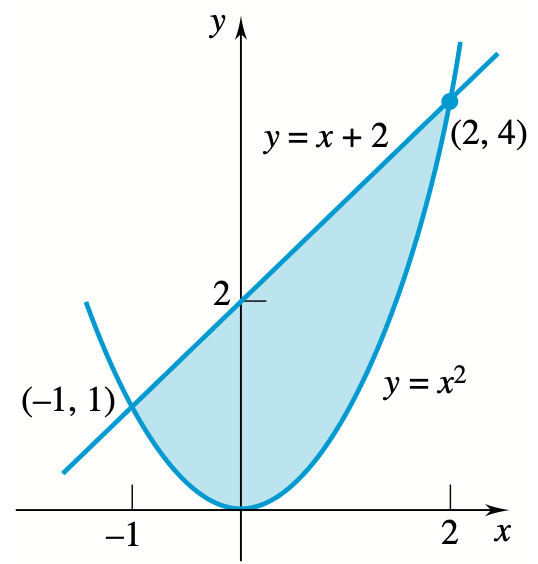
\includegraphics[width=.95\textwidth]{pics/areas-3.png}
  \end{minipage}
  \end{example}

  Hemos establecido la fórmula~\eqref{eq:area entre dos curvas} suponiendo que $f$ y $g$ son ambas no negarivas, pero esta hipótesis es innecesaria. La fórmula es válida para cualquier región $\Omega$ que tenga a $y=f(x)$ como frontera superior y a $y=g(x)$ como frontera inferior.
  Para ver esto, tomemos $\Omega$ como la figura de la izquierda y $\Omega'$ como la figura de la derecha:

  \begin{center}
    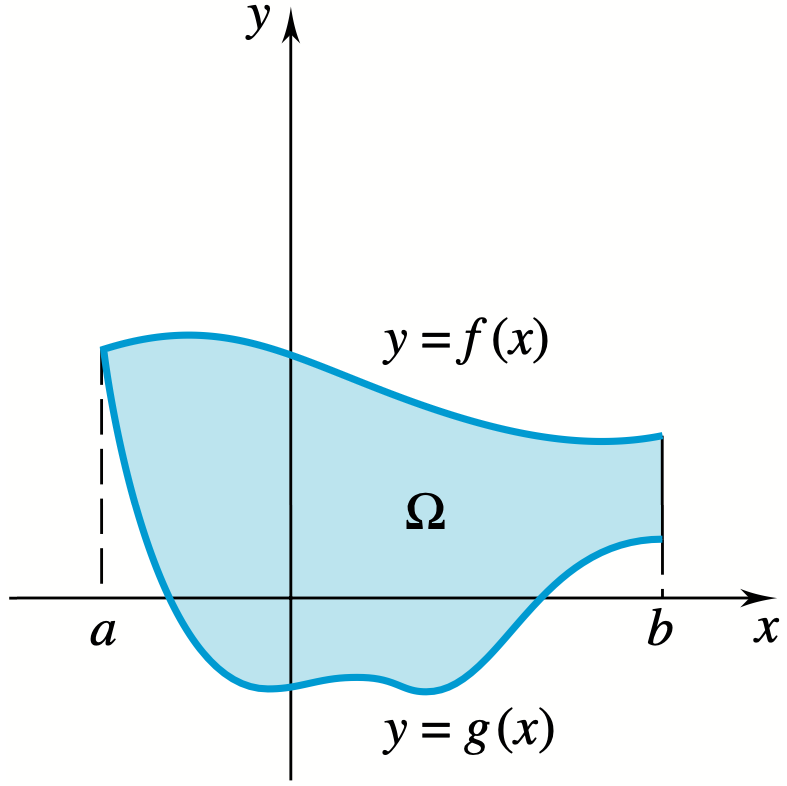
\includegraphics[width=.4\textwidth]{pics/areas-4a.png}
    \hfil
    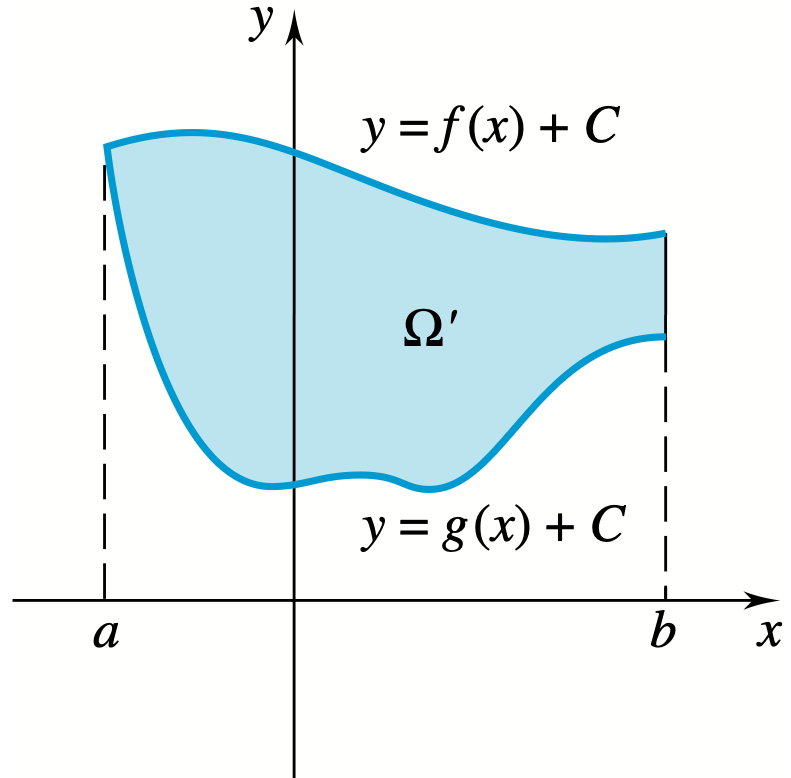
\includegraphics[width=.4\textwidth]{pics/areas-4b.png}
  \end{center}

  La figura $\Omega'$ es la misma que $\Omega$, pero trasladada hacia arriba $C$ unidades, y por lo tanto tienen la misma área. Entonces
  \[
  \area(\Omega)=\area(\Omega')
  =\int_a^b \Big[\big(f(x)+C\big)-\big(g(x)+C\big)\Big]\dx
  =\int_a^b \Big[f(x)-g(x)\Big]\dx.
  \]

  \begin{example}
    Consideramos ahora el problema de hallar el área de la figura de la derecha.

    \noindent
    \begin{minipage}{.55\textwidth}
      Usando la fórmula~\eqref{eq:area entre dos curvas} tenemos:
      \begin{align*}
        \area(\Omega) 
        &= \int_{\pi/4}^{5\pi/4} \big[\sen x-\cos x]\dx 
        \\
        &= \Big[-\cos x-\sen x\Big]_{\pi/4}^{5\pi/4}
        \\ 
        &= 2\sqrt{2}.
      \end{align*}
    \end{minipage}
    \begin{minipage}{.44\textwidth}
      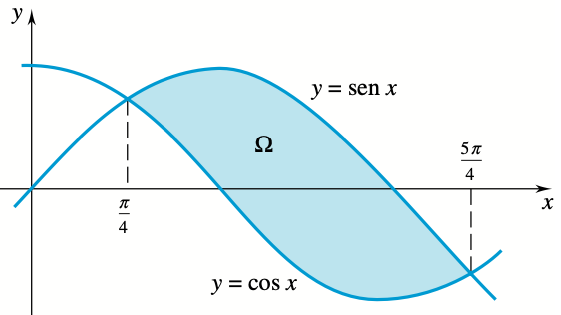
\includegraphics[width=.95\textwidth]{pics/areas-5.png}
    \end{minipage}    
  \end{example}

  \begin{example}
    Consideramos ahora el problema de hallar el área comprendida entre la curva $y=4x$ y la curva $y=x^3$, desde $x=-2$ hasta $x=2$.

    \noindent
    \begin{minipage}{.55\textwidth}
      Observamos que $y=x^3$ es la frontera \emph{superior} entre $x=-2$ y $x=0$, mientras que $y=x^3$ es la frontera \emph{inferior} entre $x=0$ y $x=2$.
      Luego,
      \begin{align*}
        \area
        &= 
        \int_{-2}^0 \big[x^3-4x\big]\dx 
        +
        \int_0^2 \big[4x-x^3\big]\dx 
        \\
        &= 
        \Big[\frac{x^4}4-2x^2\Big]_{-2}^0
        +
        \Big[4x-x^3\Big]_0^2 
        \\
        &= \big[0-(-4)\big]+[4-0]=8
      \end{align*}
    \end{minipage}
    \begin{minipage}{.44\textwidth}
      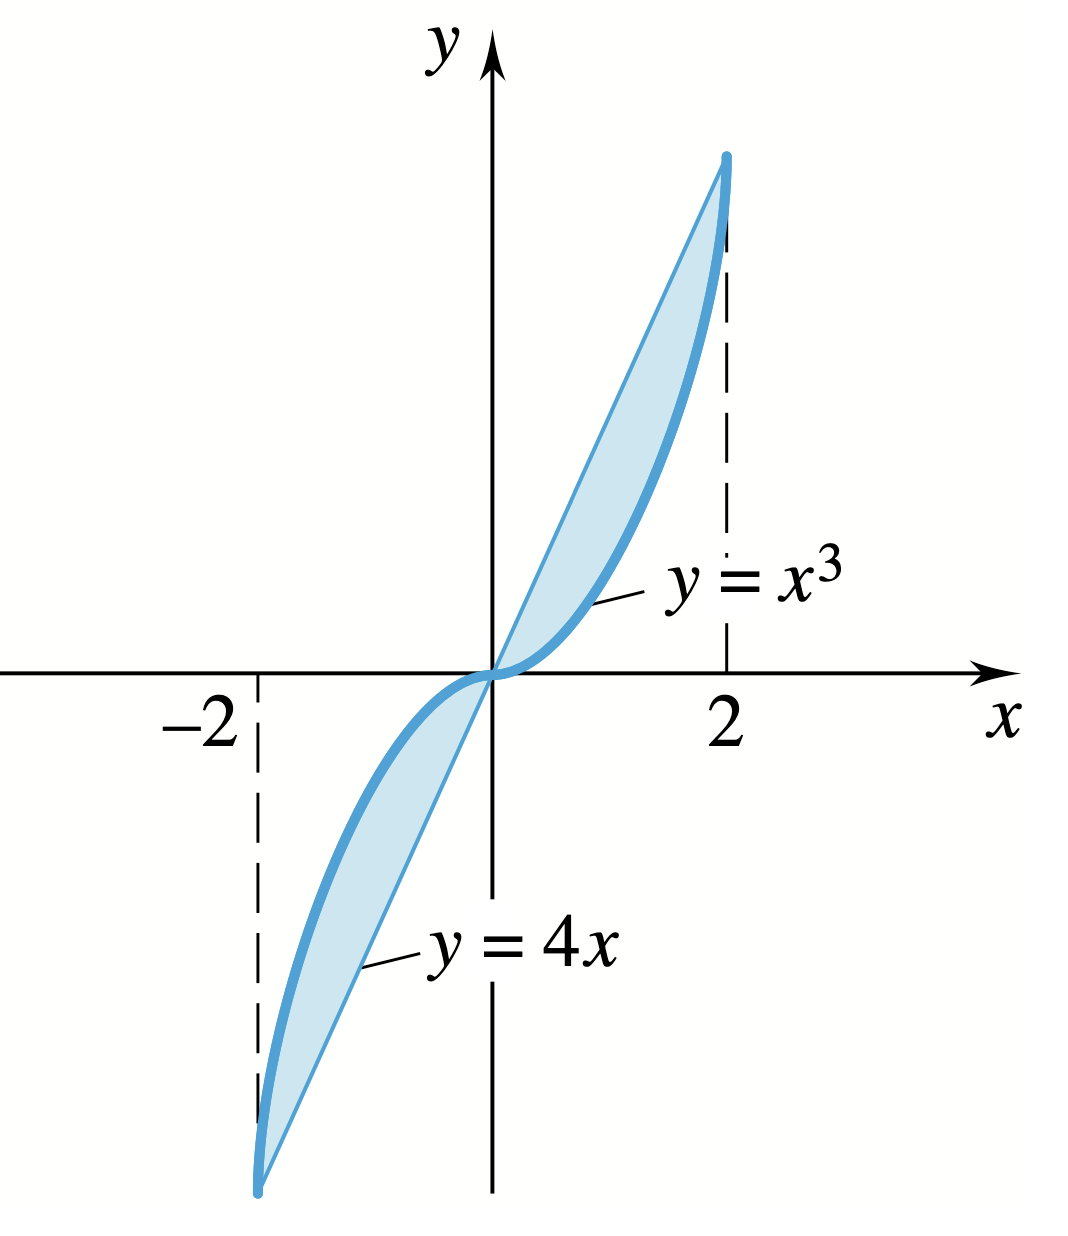
\includegraphics[width=.95\textwidth]{pics/areas-6.png}
    \end{minipage}    
  \end{example}

\subsubsection*{Ejercicios de la sección~\getcurrentref{chapter}.\getcurrentref{section}}

\begin{enumerate}
  \item Dibujar la región limitada por las curvas y calcular su área.
\begin{multicols}{2}
  \begin{enumerate}
    \item $\D y= \sqrt x$,\quad $\D y= x^2$.
    \item $\D y= 8-x^2$,\quad $\D y= x^2 $.
    \item $\D y= 5-x^2$,\quad $\D y= 3-x $.
    \item $\D y^2=2x$,\quad $\D x-y=4  $.
    \item $\D x-y^2+3=0 $,\quad $\D x-2y=0  $.
  \end{enumerate}
  
\end{multicols}
\end{enumerate}  


\section{Integrales indefinidas}

Consideremos una función continua $f$. Si $F$ es una antiderivada de $f$ en $[a,b]$, entonces
\[
\int_a^b f(x)\dx = \Big[F(x)\Big]_a^b = F(b)-F(a).
\]
Si $C$ es una constante, 
\[
  \Big[F(x)+C\Big]_a^b 
  = \big[F(b)+C\big]-\big[F(a)+C\big]= F(b)-F(a)
  = \Big[F(x)\Big]_a^b = \int_a^b f(x)\dx.
\]
Esto es así porque $F(x)+C$ es también una antiderivada de $f$ ya que
\[
\dd[]{}{x} \big(F(x)+C\big) = F'(x) = f(x).
\]
Y además, \emph{todas} las antiderivadas de $f$ son de la forma $F(x)+C$, con $C$ una constante.

Si no tenemos un interés especial en el intervalo $[a,b]$ y sólo queremos resaltar el hecho que $F$ es una antiderivada de $f$ para algún intervalo, entonces omitiremos $a$ y $b$ y simplemente escribiremos
\[
\int f(x)\dx = F(x)+C.
\]
Cuando se expresan de este modo, las antiderivadas se llaman \emph{integrales indefinidas}.
La consstante $C$ se denomina \emph{constante de integración}; es una constante \emph{arbitraria} porque se le puede asignar cualquier valor real.

La integral indefinida de una función $f$, es $\int f(x)\dx$, y es una \emph{familia} de funciones: es la familia de \emph{todas} las antiderivadas de $f$. Por ejemplo:
\[
\int x^2\dx = \frac{x^3}{3} + C 
\qquad\text y \qquad
\int \sqrt{s}\ds = \frac23 s^{3/2}+C.
\]
En base a la tabla de derivadas y a los ejercicios del capítulo anterior tenemos la siguiente tabla de integrales indefinidas:

\begin{multicols}{2}
  $\D \int x^\alpha \dx = \frac{x^{\alpha+1}}{\alpha+1} + C$, si $\alpha\neq -1$
  
  $\D \int \frac1x\dx = \ln|x| + C$
  
  $\D \int a^x \dx = \frac{a^x}{\ln a}  + C$, si $a>0$
  
  $\D \int \sen x\dx = -\cos x + C$
  
  $\D \int \cos x \dx = \sen x + C$
  
  $\D \int \sec^2 x\dx = \tan x + C$
  
  $\D \int \cosec^2 x\dx = \cot x + C$
  
  $\D \int \senh x \dx = \cosh x + C$
  
  $\D \int \cosh x \dx = \senh x + C$
  
\end{multicols}

Las propiedades de linealidad de la integral definida son también válidas para la integral indefinida:
\[
\int c\, f(x)+g(x)\dx = c \int f(x)\dx + \int g(x)\dx.
\]
Así, por ejemplo
\[
\int 3x^5 + 6 \sen x \dx = \frac{x^6}2 - 6 \cos x + C.
\]

\begin{example}
  Hallar $f$ sabiendo que $\D f'(x)=x^3+2$ y $f(0)=1$.

  Dado que $f'$ es la derivada de $f$, $f$ es una antiderivada de $f'$. Luego
  \[
  f(x)=\int (x^3+2)\dx = \frac{x^4}{4}+2x+C ,
  \]
  para algún valor de la constante $C$.
  Para hallar $C$ usaremos el hecho que $f(0)=1$:
  \[
  1=f(0)=\frac{0^4}{4}+2\cdot 0+C = C, 
  \]
  y obtenemos que $C=1$. Luego
  $\D f(x)= \frac{x^4}{4}+2x+1$.
\end{example}

\begin{example}\label{ej:velocidad}
  Consideremos un problema de movimiento.
  Un objeto se mueve a lo largo de un eje de coordenadas con una velocidad de 
  \[
  v(t)=2-3t+t^2\text{\ \ unidades por segundo.}
  \]
  Su posición inicial (posición en el instante $t=0$) es de 2 unidades a la derecha del origen.
  Hallar la posición del objeto 4 segundos más tarde.

  Sea $s(t)$ la (coordenada de la) posición del objeto en el instante $t$.
  Sabemos que $s(0)=2$ y que $s'(t)=v(t)$, luego
  \[
  s(t)=\int v(t)\dt = \int (2-3t+t^2 )\dt = 2t -\frac32 t^2 +\frac{t^3}3 + C.
  \]
  Para conocer la constante $C$ utilizaremos que $s(0)=2$:
  \[
  2=s(0)=2\cdot 0 -\frac32 0^2 +\frac{0^3}3 + C = C.
  \]
  Luego $C=2$ y la posición del objeto a tiempo $t$ es $\D 2t -\frac32 t^2 +\frac{t^3}3 +2$. A tiempo $t=4$ es 
  \[
  s(4)=2\cdot 4 -\frac32 4^2 +\frac{4^3}3 +2=\frac{22}3.
  \]
  Pasados 4 segundos se encuentra a $\D\frac{22}3$ unidades a la derecha del origen.
  En la figura se reresenta esquemáticamente el movimiento del objeto.

  \begin{center}
    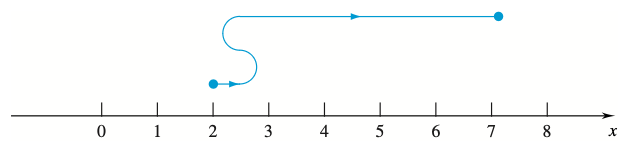
\includegraphics[width=.7\textwidth]{pics/movimiento.png}
  \end{center}

\end{example}

\subsubsection*{Ejercicios de la sección~\getcurrentref{chapter}.\getcurrentref{section}}

\begin{enumerate}
  \item Calcular las siguientes integrales indefinidas:
\begin{multicols}{2}
  \begin{enumerate}
    \item $\D \int \frac{1}{x^4} \dx$
    \item $\D \int \big(ax+b\big) \dx$
    \item $\D \int \frac{1}{\sqrt{1+x}} \dx$
    \item $\D \int \bigg(\frac{x^3-1}{x^2}\bigg) \dx$
    \item $\D \int \bigg(\sqrt{x}-\frac{1}{\sqrt{x}}\bigg) \dx$
    \item $\D \int \big(\sen x+\cos x\big) \dx$
    \item $\D \int \big(\senh x+\cosh x\big) \dx$
    \item $\D \int \frac{g'(x)}{g(x)^2} \dx$
  \end{enumerate}
\end{multicols}

\item Hallar $f$ a partir de la información dada:
\begin{multicols}{2}
  \begin{enumerate}
    \item $f'(x)=2x-1$,\ \ $f(3)= 0$
    \item $f'(x)=ax+b$,\ \ $f(0)=c $
    \item $f'(x)=\sen x$,\ \ $f(0)= 2$
    \item $f'(x)=\cos x$,\ \ $f(\pi )=3 $
  \end{enumerate}
\end{multicols}

\item Un objeto se mueve a lo largo de un eje de coordenadas con una velocidad de $v(t)=6t^2-6$ metros por segundo. Su posición inicial (posición en tiempo $t=0$) es 2 unidades a la izquierda del origen.
\begin{enumerate}
  \item Hallar la posición del objeto $3$ segundos más tarde.
  \item Representar esquemáticamente el movimiento del objeto como en el Ejemplo~\ref{ej:velocidad}.
  \item ?`Cuál es la distancia entre la posición del objeto a tiempo $t=0$ y la posición a tiempo $t=3$?
  \item ?`Cuál es la distancia total recorrida por el objeto entre tiempo $t=0$ y $t=1$?
\end{enumerate}
\end{enumerate}    


\section{Integración por sustitución}

La integración por sustitución, también conocida como \emph{cambio de variables} no es otra cosa que la utilización de la regla de la cadena en sentido inverso para hallar una antiderivada.
Recordamos que si $F$ y $g$ son diferenciables, con $F'(u)=f(u)$, entonces
\[
(F\circ g)'(x) = \dd[]{}{x} F\big(g(x)) = F'(g(x))\, g'(x) = f(g(x))\, g'(x).
\]
Por lo tanto, 
\[
\int_a^b f(g(x))\, g'(x)\dx = \Big[F(g(x))\Big]_a^b = F(g(b))-F(g(a)).
\]

Por ejemplo:
\[
\int_0^\pi \cos(x^2+1)\, 2x \dx = \Big[\sen(x^2+1)\Big]_0^\pi = 
\sen(\pi^2+1)-\sen(0^2+1).
\]
En el ejemplo recién presentado hemos detectado que $\cos(u)$ es la derivada de $\sen(u)$, y que $2x$ es la derivada de $u=x^2+1$.

También podemos usar la regla de sustitución para calcular una integral indefinida. Esto es lo más usual, y suele hacerse de la siguiente manera:
\[
\int f(\underbrace{g(x)}_u) \, \underbrace{g'(x)\dx}_{\du} = 
\int f(u) \du = F(u)+C = F(g(x))+C.
\]
Por ejemplo, 
\[
\int (\underbrace{x^2-1}_u)^4\, \underbrace{2x\dx}_{\du} = \int u^4 \du 
= \frac{u^5}5 + C
= \frac{(x^2-1)^5}5 + C.
\]
Podemos verificar esto derivando la última expresión:
\[
\dd[]{}{x} \left(\frac{(x^2-1)^5}5 + C\right) =
\frac{5(x^2-1)^4\,2x}5 = (x^2-1)^4\, 2x.
\]

\begin{example}
  Calcular $\D \int \sen x\,\cos x\dx$.

  El problema aquí es \emph{darse cuenta} qué parte de la fórmula puede ser $u$ y qué parte será $\du$. 
  Si recordamos que $\sen'x = \cos x$, vemos que podemos hacer la sustitución $u=\sen x$ y $\du = \cos x\dx$, entonces
  \[
  \int \underbrace{\sen x}_u\,\underbrace{\cos x\dx}_{\du} = \int u \du = \frac{u^2}2 + C 
  \underbrace{=}_{u=\sen x} \frac{\sen^2 x}{2}+ C.
  \]
  Conviene siempre hacer la verificación:
  \[
  \dd[]{}{x}\Big(\frac{\sen^2 x}{2}+ C\Big) = \frac{2 \sen x \, \cos x}2 = \sen x\,\cos x.
  \]
\end{example}

\begin{example}
  Calcular $\D \int \frac{1}{(3+5x)^2}\dx$. 
  
  Aquí no es tan obvio que aparezca $u$ y $\du$, pero con un poco de práctica se aprende.
  Si tomamos $u=(3+5x)$, entonces $\du = 5\dx$, pero ese $5$ no está. Usando la linealidad de la integral, como $5$ es una constante, podemos hacer lo siguiente:
  \begin{align*}
    \int \frac{1}{(3+5x)^2}\dx &= \int \frac55 \frac{1}{(3+5x)^2}\dx
    = \frac15 \int \frac{1}{(\underbrace{3+5x}_u)^2} \underbrace{5\dx}_{\du}
    = \frac15 \int \frac{1}{u^2} \du 
    \\
    &= \frac15 \int u^{-2} \du
    = \frac15 \Big(\frac{u^{-1}}{-1}+C\Big)
    = \frac15 \Big(-\frac{1}{u}+C\Big)
    \\
    &= -\frac{1}{5u}+\frac{C}5
    = -\frac{1}{5u}+C'
    = -\frac{1}{5(3+5x)^2}+C'.
  \end{align*}
\end{example}

Si tenemos que calcular una integral definida utilizando el método de sustitución, hay dos formas (por lo menos).
La primera es la siguiente: calcular primero la integral indefinida (basta con una antiderivada) y luego utilizarla para integrar.

\begin{example}
  Calcular $\D \int_0^2 (x^2-1) \, (x^3-3x+2)^3 \dx$.

  Hacemos aquí la sustitución $u=x^3-3x+2$ y $\du = 3x^2-3\dx=3(x^2-1)\dx$,
  y miramos la integral indefinida:
  \begin{align*}
    \int (x^2-1) \, (x^3-3x+2)^3 \dx &= \frac13 \int  (x^3-3x+2)^3\, 3(x^2-1) \dx
    \\
    &=\frac13\int u^3 \du = \frac{u^4}{12} + C = \frac{(x^3-3x+2)^4}{12} + C.
  \end{align*}
  Es decir, hemos encontrado que $\frac{(x^3-3x+2)^4}{12}$ es una antiderivada del integrando.
  Luego
  \begin{align*}
    \int_0^2 (x^2-1) \, (x^3-3x+2)^3 \dx 
    &= \Big[
      \frac{(x^3-3x+2)^4}{12}
      \Big]_0^2
      \\
      &= \frac{(2^3-3\cdot 2+2)^4}{12} - \frac{(0^3-3\cdot 0+2)^4}{12}
      \\
      &=   \frac{(8-6+2)^4}{12} - \frac{2^4}{12} = 20.
  \end{align*}  
\end{example}

La segunda forma será vista luego del siguiente teorema:

\begin{theorem} 
  Si $f$ es continua y $g$ es tal que $g'$ es continua, entonces
  \[
  \int_a^b f(g(x))\, g'(x)\dx = \int_{g(a)}^{g(b)} f(u)\du.
  \]
\end{theorem}

\begin{proof}
  Sea $F$ una antiderivada de $f$. Entonces $F'(u)=f(u)$ y 
  \begin{align*}
    \int_a^b f(g(x))\, g'(x)\dx 
    &= \int_a^b F'(g(x))\, g'(x)\dx \\
    &= \Big[ F(g(x))\Big]_a^b = F(g(b))-F(g(a)) 
    \\
    &= \Big[ F(u)\Big]_{g(a)}^{g(b)} = \int_{g(a)}^{g(b)} f(u) \du. 
    \qedhere
  \end{align*}
\end{proof}

Lo importante a notar en esta fórmula, es que si aplicamos la regla de sustitución en una integral \emph{definida}, también hay que sustituir en los extremos de integración.

\begin{example}
  Calcular $\D\int_0^{1/2} \cos^3 \pi x\,\sen\pi x\dx$.
  Hacemos la sustitución $u=\cos\pi x$ y $\du = -\pi \sen\pi x \dx$:
  \begin{align*}
    \int_0^{1/2} \cos^3 \pi x\,\sen\pi x\dx 
    &= -\frac1\pi \int_0^{1/2} \cos^3 \pi x\,(-\pi\,\sen\pi x)\dx \\
    &= -\frac1\pi \int_{\cos \pi 0}^{\cos \pi 1/2} u^3 \du 
    = -\frac1\pi \int_{1}^{0} u^3 \du \\
    &= -\frac1\pi  \Big[\frac{u^4}{4}\Big]_{1}^{0} 
    = -\frac1\pi  \Big[\frac{0^4}{4}-\frac{1^4}{4}\Big]_{1}^{0} 
    = -\frac1\pi  \Big[0-\frac{1}{4}\Big]
    = \frac{1}{4\pi}.
  \end{align*}
\end{example}

Para finalizar la sección, veamos un último ejemplo de sustitución en una integral indefinida 

\begin{example}
  Calcular $\D\int 2x \sqrt{x-1}\dx$.

  Aquí tenemos $x$ fuera de la raíz y $x-1$ dentro de la raíz. Parece que no podríamos hacer nada. Sin embargo, si hacemos la sustitución $u=x-1$ (nos queda $x=u+1$) y $\du = \dx$:
  \begin{align*}
    \int 2\underbrace{x}_{u+1} \sqrt{\underbrace{x-1}_u}\underbrace{\dx}_{\du}
    &= \int 2 (u+1)\sqrt{u}\du = 2 \int u^{3/2}+u^{1/2}\du
    \\
    &= 2\Big[ \frac{u^{5/2}}{5/2} + \frac{u^{3/2}}{3/2}\Big]
    = \frac45 u^{5/2} + \frac43 u^{3/2}
    =  \frac45 (x-1)^{5/2} + \frac43 (x-1)^{3/2}.
  \end{align*}
\end{example}

\subsubsection*{Ejercicios de la sección~\getcurrentref{chapter}.\getcurrentref{section}}

\begin{enumerate}
  \item Calcular las siguientes integrales indefinidas mediante el método de sustitución:

\begin{multicols}{2}
  \begin{enumerate}
    \item $\D \int \frac{1}{(2-3x)^2} \dx$.
    \item $\D \int \sqrt{ax+b} \dr$.
    \item $\D \int \frac{t}{(4t^2+9)^2} \dt$.
    \item $\D \int x^2 (1+x^3)^{1/4} \dx$.
    \item $\D \int \frac{b^3 \, x^3}{\sqrt{1-a^4x^4}} \dx$.
    \item $\D \int \frac{1}{4x+6}\dx$.
    \item $\D \int \frac{x^3}{1+x^4}\dx$.
    \item $\D \int e^{ax+b}\dx$.
    \item $\D \int x^3 e^{x^4+1}\dx$.
  \end{enumerate}
\end{multicols}

\item Calcular las siguientes integrales definidas mediante el método de sustitución:

\begin{multicols}{2}
  \begin{enumerate}
    \item $\D \int_{0}^{1} x(x^2+1)^3 \dx$.
    \item $\D \int_{-1}^{1} \frac{r}{(1+r^2)^4} \dr$.
    \item $\D \int_{0}^{3} \frac{r}{\sqrt{r^2+16}}  \dr$.
    \item $\D \int_{0}^{a} y\sqrt{a^2-y^2} \dy$.
  \end{enumerate}
\end{multicols}

\item Calcular las siguientes integrales indefinidas utilizando el cambio de variables indicado:

\begin{multicols}{2}
  \begin{enumerate}
    \item $\D \int x \sqrt{x+1} \dx $, $u = x+1$.
    \item $\D \int x \sqrt{2x-1} \dx $, $u = 2x-1$.
    \item $\D \int t\,(2t+3)^8 \dt $, $u = 2t+3$.
    \item $\D \int \frac{x+3}{\sqrt{x+1}}\dx $, $u = x+1$.
  \end{enumerate}
\end{multicols}
\end{enumerate}  

\section{Integración por partes}
% sección 9.3 de Noriega

En la sección anterior hemos visto cómo la regla de la cadena para la derivada de una composición nos permite calcular derivadas de funciones más complejas.
También hay una regla de integración asociada con la regla de la derivada de un producto.

Sean $u$ y $v$ dos funciones derivables. Por la Proposición~\ref{P:derivada del producto} tenemos que
\[
(uv)'=u'v + u v',
\]
o sea 
\[
  u'v =(uv)'- u v'.
\]
Entonces resulta que 
$$
\int u'v \dx = \int (uv)' \dx - \int u v'\dx.
$$

Tenemos entonces el siguiente Teorema.

\begin{theorem}[Integración por partes]
  Si $u$ y $v$ son funciones diferenciables tales que $u'$ y $v'$ son continuas, entonces 
  \[
  \int_a^b u'(x)v(x) \dx = \Big[u(x)v(x)\Big]_a^b - \int_a^b u(x) v'(x)\dx,
  \]
  es decir,
  \[
  \int_a^b u'(x)v(x) \dx 
  = u(b)v(b)-u(a)v(a) - \int_a^b u(x) v'(x)\dx.
  \]
\end{theorem}

\begin{proof}
  Por la regla de la derivada del producto, Proposición~\ref{P:derivada del producto} tenemos que $(uv)'(x)=u'(x)v(x) + u(x) v'(x)$. Luego, $(uv)(x)=u(x)v(x)$ es una antiderivada de $u'(x)v(x) + u(x) v'(x)$. Por la linealidad de la integral y por la regla de Barrow tenemos que
  \begin{align*}
  \int_a^b u'(x)v(x) \dx+ \int_a^b u(x) v'(x) \dx
  &=\int_a^b u'(x)v(x) + u(x) v'(x) \dx
  \\
  &= \int_a^b (uv)'(x)\dx 
  = \Big[(uv)(x)\Big]_a^b  
  \\
  &= \Big[u(x)v(x)\Big]_a^b  
  = u(b)v(b)-u(a)v(a),
  \end{align*}
  de donde se deduce inmediatamente la afirmación del teorema.
\end{proof}

Otra forma de escribir la \emph{fórmula de integración por partes} es la siguiente:
$$
\int u'v \dx = uv - \int u v'\dx,
$$
y si llamamos $\du = u'(x)\dx$ y $\dv = v'(x)\dx$ tenemos
$$
\int v \du = uv - \int u \dv.
$$

Veamos cómo se puede aplicar esta regla en ejemplos concretos.

\begin{example}
  Calcular $\D\int x\,\ln x\dx$.

  Aquí hacemos $u=\ln x$ y $v'=x$. Luego $\D u'=\frac1x$ y $\D v=\frac{x^2}2$. Luego
  \[
  \int x \ln x\dx 
  = \ln x \, \frac{x^2}2 - \int \frac1x \frac{x^2}{2}\dx
  = \ln x \, \frac{x^2}2 - \int \frac{x}{2}\dx
  = \ln x \, \frac{x^2}2 - \frac{x^2}{4} + C.
  \]  
\end{example}

\begin{example}
  Calcular $\D \int x e^x\dx$.

  En este ejemplo, la idea es aprovechar que $\dd[]{x}{x}=1$ y que $\dd[]{e^x}{x}=e^x$. Entonces tomamos $u=x$, y $v'=e^x$. Luego, $u'=1$ y $v=e^x$:
  \[
  \int x\, e^x\dx = x\,e^x - \int 1 e^x\dx = x\, e^x - e^x+C = (x-1)e^x+C.
  \]
\end{example}

\begin{example}
  Calcular $\D \int x^2 e^x\dx$.

  En este ejemplo, la idea es repetir dos veces la fórmula para poder \emph{deshacernos} de la potencia de $x$. Tomamos primero $u=x^2$, y $v'=e^x$. Luego, $u'=2x$ y $v=e^x$:
  \[
  \int x^2\, e^x\dx 
  = x^2\,e^x - \int 2x e^x\dx 
  = x^2\,e^x - 2\int x e^x\dx .
  \]
  Llegado a este punto nos tocaría aplicar nuevamente la integración por partes en el último término, pero como lo hemos hecho en el ejemplo anterior, podemos copiar la fórmula de allí.
  \[
  \int x^2\, e^x\dx 
  = x^2\,e^x - 2\int x e^x\dx 
  = x^2\,e^x - 2(x\, e^x - e^x) + C
  = (x^2-2x+2)\,e^x + C.
  \]
\end{example}

Veamos un último ejemplo.

\begin{example}
  Calcular $\D \int e^x\, \cos x \dx$.

  Aquí integraremos por partes dos veces. Primero escribimos
  $u=e^x$ y $v'=\cos x$, con $u'=e^x$ y $v=\sen x$. Esto nos da
  \[
  \int e^x\,\cos x \dx 
  = e^x \,\sen x - \int e^x \,\sen x\dx .
  \]
  Ahora hacemos integración por partes en $\D \int e^x \, \sen x \dx$.
  En este caso, tomamos $u=e^x$ y $v'=\sen x$, con $u'=e^x$ y $v=-\cos x$. Luego
  \[
  \int e^x\,\sen x \dx 
  = e^x (-\cos x) - \int e^x (-\cos x)\dx 
  = -e^x \,\cos x + \int e^x \, \cos x \dx .
  \]
  Juntando todo,
  \begin{align*}
    \int e^x\,\cos x \dx 
    &= e^x \,\sen x -\Big[-e^x \,\cos x + \int e^x \, \cos x \dx \Big]\\
    &= e^x \,\sen x +e^x \,\cos x - \int e^x \, \cos x \dx .
  \end{align*}
  Es decir
  \[
    \int e^x\,\cos x \dx 
    = e^x\big(\sen x+\cos x) - 
    \int e^x\,\cos x \dx .
  \]
  Por lo tanto 
  \[
    2\int e^x\,\cos x \dx 
    = e^x\big(\sen x+\cos x),
  \]
  y finalmente 
  \[
    \int e^x\,\cos x \dx 
    = \frac{e^x}2\big(\sen x+\cos x) + C.
  \]
\end{example}



\subsubsection*{Ejercicios de la sección~\getcurrentref{chapter}.\getcurrentref{section}}

\begin{enumerate}
  \item Calcular las siguientes integrales:
\begin{multicols}{2}
  \begin{enumerate}
    \item $\D \int x\,e^{-x} \dx$.
    \item $\D \int_0^2 x \, 2^x  \dx$.
    \item $\D \int x^2\, e^{-x^3} \dx$.
    \item $\D \int x \, \ln x^2 \dx$.
    \item $\D \int_0^1 x^2\, e^{-x} \dx$.
    \item $\D \int \frac1{x\, (\ln x)^3} \dx$.
    % \item $\D \int  \dx$.
  \end{enumerate}
  
\end{multicols}
\item Hallar el área de la región limitada por la gráfica de $f$ y el eje $x$:
\begin{multicols}{2}
  \begin{enumerate}
    \item $f(x)=\arcsen x$, $x\in[0,1/2]$.
    \item $f(x)=x\,e^{-2x}$,  $x\in[0,2]$.
  \end{enumerate}
\end{multicols}
\end{enumerate}  


\section{Algunas propiedades adicionales de la integral}

En esta sección veremos algunas propiedades generales importantes de la integral definida. En todos los resultados presentados en esta sección estamos suponiendo que $a<b$.

\begin{lemma}\label{L:integral ge 0}
  Si $f$ es continua a trozos y $f(x)\ge 0$, para todo $x\in [a,b]$, entonces 
  \[
  \int_a^b f(x)\dx \ge 0.
  \]
\end{lemma}

\begin{proof}
  Hacemos la demostración para el caso en que $f$ es continua.
  Como $f$ es continua en $[a,b]$, alcanza su mínimo, digamos en un punto $x_m$, donde $f(x_m)\ge 0$ por hipótesis. Tomemos ahora la partición $P=\{x_0=a<x_1=b\}$.
  Luego 
  \[
  L(P,f)=f(x_m) (b-a)=\ell \ge 0.
  \]
  Por lo tanto la integral, que es un número mayor o igual a todas las sumas inferiores tiene que ser también mayor o igual que $\ell\ge0$ y por lo tanto es no negativa.
\end{proof}

\begin{lemma}\label{L:integral > 0}
  Si $f$ es continua a trozos y $f(x)> 0$, para todo $x\in [a,b]$, entonces
  \[
  \int_a^b f(x)\dx > 0.
  \]
\end{lemma}

\begin{proof}
  Hacemos la demostración para el caso en que $f$ es continua.
  Como $f$ es continua en $[a,b]$, alcanza su mínimo, digamos en un punto $x_m$, donde $f(x_m)>0$ por hipótesis. Tomemos ahora la partición $P=\{x_0=a<x_1=b\}$.
  Luego 
  \[
  L(P,f)=f(x_m) (b-a)=\ell > 0.
  \]
  Por lo tanto la integral, que es un número mayor o igual a todas las sumas inferiores tiene que ser también mayor o igual que $\ell>0$ y por lo tanto es positiva.
\end{proof}

\begin{proposition}\label{P:integral monotona}
  Si $f$ y $g$ son continuas a trozos y $f(x)\le g(x)$ para todo $x\in[a,b]$, entonces
  \[
  \int_a^b f(x)\dx 
  \le \int_a^b g(x)\dx 
  \]
\end{proposition}

\begin{proof}
  Aplicar el Lema~\ref{L:integral ge 0} a la función $h(x)=g(x)-f(x)$.
\end{proof}

\begin{proposition}
  Si $f$ y $g$ son continuas a trozos y $f(x) < g(x)$ para todo $x\in[a,b]$, entonces
  \[
  \int_a^b f(x)\dx 
  < \int_a^b g(x)\dx 
  \]
\end{proposition}

\begin{proof}
  Aplicar el Lema~\ref{L:integral > 0} a la función $h(x)=g(x)-f(x)$.
\end{proof}

\begin{theorem}[Teorema del Valor Medio del Cálculo Integral]\label{T:TVM-integral}
  Si $f$ es una función continua en $[a,b]$ entonces existe $c\in(a,b)$ tal que 
  \[
  \int_a^b f(x)\dx = f(c)\cdot(b-a).
  \]
\end{theorem}

\begin{proof}
  Si $M$ y $m$ denotan el máximo de la función $f$ en el intervalo $[a,b]$, entonces $m\le f(x)\le M$ para todo $x\in[a,b]$, luego, por la última proposición
  \[
  \int_a^b m\dx
  \le \int_a^b f(x)\dx
  \le \int_a^b M\dx.
  \]
  Como la integral de una constante es la constante por la longitud del intervalo, tenemos que
  \[
    m\cdot(b-a)
    \le \int_a^b f(x)\dx
    M\cdot(b-a).
  \]
  Dividiendo por $b-a>0$ tenemos
  \[
  m \le \frac{\int_a^b f(x)\dx}{b-a}\le M.
  \]
  Es decir que el número $d=\frac{\int_a^b f(x)\dx}{b-a}$ está entre el máximo y el mínimo de $f$. Luego, por el teorema del valor intermedio para funciones continuas, existe $c\in(a,b)$ tal que $f(c)=d$ es igual a ese número. Luego
  \[
  f(c) = \frac{\int_a^b f(x)\dx}{b-a},
  \]
  o, lo que es lo mismo
  \[
  \int_a^b f(x)\dx = f(c)\cdot(b-a).
  \qedhere
  \]
\end{proof}

\begin{remark}
  La cantidad $\D \frac{\int_a^b f(x)\dx}{b-a}$ se llama \emph{valor medio} o \emph{promedio} de $f$ en el intervalo $[a,b]$. Coincide con el valor por el que hay que multiplicar la longitud del intervalo para obtener el valor de la integral de $f$.
\end{remark}

\begin{theorem}[Segundo teorema del valor medio para integrales]
Si $f$ y $g$ son funciones continuas en $[a,b]$ y $g$ es no negativa, entonces existe $c\in(a,b)$ para el cual se verifica que
\[
\int_a^b f(x)g(x)\dx = f(c) \int_a^b g(x)\dx.
\] 
\end{theorem}

\begin{proof}
  La demostración de este teorema es similar a la del teorema anterior. 
  Si $M$ y $m$ denotan el máximo de la función $f$ en el intervalo $[a,b]$, entonces $m\le f(x)\le M$ para todo $x\in[a,b]$, y como $g(x)\ge 0$ para todo $x$, se cumple que
  \[
  m\,g(x)\le f(x)g(x)\le M\,g(x), \quad\text{para todo $x\in[a,b]$.}
  \]
  Por la Proposición~\ref{P:integral monotona}
  \[
  \int_a^b m\,g(x)\dx
  \le \int_a^b f(x)g(x)\dx
  \le \int_a^b M\,g(x)\dx,
  \]
  y en consecuencia,
  \[
    m\,\int_a^b g(x)\dx
  \le \int_a^b f(x)g(x)\dx
  \le M\,\int_a^b g(x)\dx.
  \]
  Como $g$ es no negativa, $\int_a^b g(x)\dx\ge 0$. 
  Si $\int_a^b g(x)\dx=0$, entonces es porque $g(x)=0$, para todo $x\in[a,b]$.
  Luego $\int_a^b f(x)g(x)\dx=0$ y el teorema se verifica para todo $c\in(a,b)$.
  
  Si $\int_a^b g(x)\dx > 0$, dividimos la última desigualdad por esta cantidad y tenemos
  \[
    m
    \le \frac{\int_a^b f(x)g(x)\dx}{\int_a^b g(x)\dx}
    \le M.
  \]
  Es decir que el número $d=\frac{\int_a^b f(x)g(x)\dx}{\int_a^b g(x)\dx}$ está entre el máximo y el mínimo de $f$. Luego, por el teorema del valor intermedio para funciones continuas, existe $c\in(a,b)$ tal que $f(c)=d$ es igual a ese número. Luego
  \[
  f(c) = \frac{\int_a^b f(x)g(x)\dx}{\int_a^b g(x)\dx},
  \]
  o, lo que es lo mismo
  \[
  \int_a^b f(x)g(x)\dx = f(c)\int_a^b g(x)\dx.
  \qedhere
  \]
\end{proof}

\begin{remark}
  La cantidad $\D\frac{\int_a^b f(x)g(x)\dx}{\int_a^b g(x)\dx}$ que aparece en la última demostración se llama valor medio o promedio \emph{ponderado por $g$} de $f$ en el intervalo $[a,b]$.
\end{remark}

De la misma manera que el valor absoluto de una suma es menor o igual que la suma de los valores absolutos:
\[
|f_1+f_2+\dots+f_n| \le |f_1|+|f_2|+\dots+|f_n| ,
\]
el valor absoluto de una integral es menor o igual que la integral del valor absoluto.

\begin{corollary}
  Si $f$ es continua a trozos en $[a,b]$ entonces
  \[
  \Big| \int_a^b f(x)\dx \Big| \le \int_a^b |f(x)|\dx.
  \]
\end{corollary}

\begin{proof}
  Dado que $\D -|f(x)|\le f(x)\le |f(x)|$, la Proposición~\ref{P:integral monotona} nos dice que
  \[
    -\int_a^b |f(x)|\dx 
    \le \int_a^b f(x)\dx 
    \le \int_a^b |f(x)|\dx .
  \]
  Este par de desigualdades equivale a la afirmación que queremos demostrar.
\end{proof}


\subsubsection*{Ejercicios de la sección~\getcurrentref{chapter}.\getcurrentref{section}}

\begin{enumerate}
  \item Supongamos que $f$ y $g$ son continuas, $a<b$ y 
\[
\int_a^b f(x)\dx > \int_a^b g(x)\dx.
\]
\begin{enumerate}
  \item ?`Se deduce necesariamente que $\int_a^b \big[ f(x)-g(x)\big]\dx > 0$?
  \item ?`Se deduce necesariamente que $f(x)>g(x)$, para todo $x\in [a,b]$?
  \item ?`Se deduce necesariamente que existe $x\in[a,b]$ tal que $f(x)>g(x)$?
  \item ?`Se deduce necesariamente que $\Big|\int_a^b f(x)\dx\Big| > \Big|\int_a^b g(x)\dx\Big| $?
\end{enumerate}

\item Supongamos que $f$ es continua, $a<b$ y 
\[
\int_a^b f(x)\dx =0.
\]
\begin{enumerate}
  \item ?`Se deduce necesariamente que $f(x)=0$, para todo $x\in [a,b]$?
  \item ?`Se deduce necesariamente que existe $x\in[a,b]$ tal que $f(x)=0$?
  \item ?`Se deduce necesariamente que $\Big|\int_a^b f(x)\dx\Big| =0 $?
  \item ?`Se deduce necesariamente que $\int_a^b |f(x)|\dx =0 $?
\end{enumerate}
\end{enumerate}


  
\section{Cálculo de volúmenes}

En esta sección utilizaremos integrales para hallar volúmenes de ciertos sólidos tridimensionales.

Para comenzar, sea $\Omega$ una región plana.
Un \emph{cilindro recto con sección transversal $\Omega$} es un sólido formado por la traslación de $\Omega$ a lo largo de una recta, o \emph{eje}, que es perpendicular a ella.

\begin{center}
  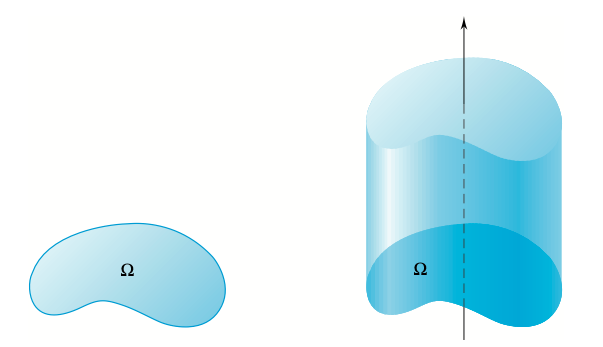
\includegraphics[width=.6\textwidth]{pics/cilindro.png}
\end{center}

Sea $A=\area(\Omega)$. Si un cilindro recto está formado por la traslación de la región $\Omega$ a lo largo de una distancia $h$, entonces el volumen del cilindro viene dado por 
\[
V = A\cdot h.
\]
Algunos ejemplos familiares son un cilindro circular recto de radio \( r \) y altura \( h \), y una caja rectangular de longitud \( l \), ancho \( w \) y altura \( h \).

\begin{center}
  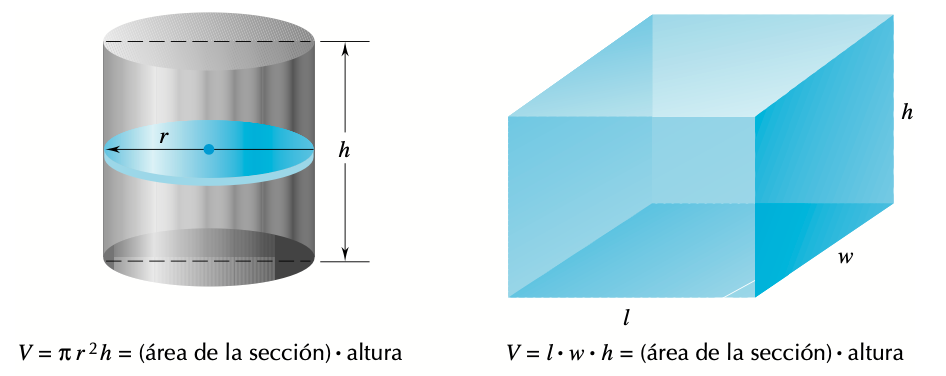
\includegraphics[width=.6\textwidth]{pics/cilindro-prisma.png}
\end{center}

\noindent
\begin{minipage}{.65\textwidth}
Para calcular el volumen de un sólido más general, introducimos un eje de coordenadas y examinamos las secciones transversales del sólido perpendiculares a dicho eje. En la figura de la derecha hemos representado un sólido y un eje de coordenadas considerado como eje \( x \).
Como en la figura, suponemos que el sólido está enteramente situado entre \( x = a \) y \( x = b \). En la figura se puede ver una sección arbitraria del sólido, perpendicular al eje \( x \). En lo sucesivo, por \( A(x) \) designamos el área de la sección transversal que tiene coordenada \( x \).

Si el área de la sección transversal, \( A(x) \), varía continuamente con \( x \), podemos hallar el volumen \( V \) del sólido mediante la integración de dicha función entre \( a \) y \( b \):
\begin{equation} \label{eq:volumen}
V = \int_a^b A(x) \, dx.
\end{equation}

\end{minipage}
\begin{minipage}{.34\textwidth}
  \begin{center}
    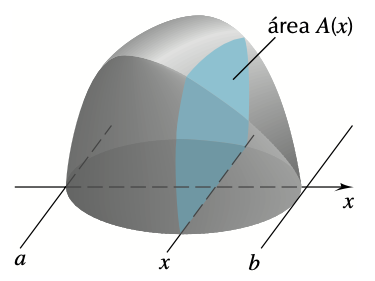
\includegraphics[width=.9\textwidth]{pics/volumen-1.png}
  \end{center}
\end{minipage}

\begin{example}
  Hallar el volumen de una pirámide cuya altura es \( h \) y cuya base es un cuadrado con lados de longitud \( r \).


  \noindent\begin{minipage}{.6\textwidth}
    Situamos el eje \( x \) perpendicular a la base, con el origen en el centro de la base. La sección transversal con coordenada \( x \) es un cuadrado. Sea \( s \) la longitud del lado de ese cuadrado. Entonces, por triángulos semejantes (ver figura), tenemos
    \[
    \frac{\frac{1}{2}s}{h - x} = \frac{\frac{1}{2}r}{h},
    \]
    y por tanto
    \[
    s = \frac{r}{h}(h - x).
    \]
  
  \end{minipage}
  \begin{minipage}{.39\textwidth}
    \begin{center}
      \includegraphics[width=.9\textwidth]{pics/piramide.png}
    \end{center}
  \end{minipage}
  
  Luego el área del cuadrado en la coordenada $x$ es $A(x) = s^2 = (r^2/h^2)(h-x)^2$.

Por lo tanto, el volumen resulta:
\begin{align*}
  V &= \int_0^h A(x) dx = \frac{r^2}{h^2} \int_0^h (h-x)^2 dx\\
&= \frac{r^2}{h^2} \left[-\frac{(h-x)^3}{3}\right]_0^h = \frac{1}{3} \pi r^2 h.
\end{align*}

\end{example}

\begin{example}
La base de un sólido es la región delimitada por la elipse
\[
\frac{x^2}{a^2} + \frac{y^2}{b^2} = 1.
\]

Hallar el volumen de dicho sólido sabiendo que la sección transversal perpendicular al eje $x$ es un triángulo isósceles con base en la región y altura igual a la mitad de la base.

\noindent\begin{minipage}{.6\textwidth}
  Sea $x$ como en la figura de la derecha. La sección transversal de coordenada $x$ es un triángulo isósceles de lado $PQ$ y altura $\frac{1}{2}PQ$. La ecuación de la elipse puede escribirse como
  \[
  y^2 = \frac{b^2}{a^2}(a^2 - x^2).
  \]
  
  Dado que
  \[
  \text{longitud de } PQ = 2y = \frac{2b}{a}\sqrt{a^2 - x^2},
  \]
  el área del triángulo isósceles será:
  \[
  A(x) = \frac{1}{2}bh = \frac{1}{2} \left(\frac{2b}{a}\sqrt{a^2 - x^2}\right) \left(\frac{b}{a}\sqrt{a^2 - x^2}\right) = \frac{b^2}{a^2}(a^2 - x^2).
  \]
\end{minipage}
\begin{minipage}{.39\textwidth}
  \begin{center}
    \includegraphics[width=.9\textwidth]{pics/volumen-2.png}
  \end{center}
\end{minipage}

Podemos hallar el volumen del sólido integrando $A(x)$ desde $x = -a$ hasta $x = a$:
\begin{align*}
V &= \int_{-a}^{a} A(x) dx = 2 \int_{0}^{a} A(x) dx \quad \text{por simetría}
\\
&= \frac{2b^2}{a^2} \int_{0}^{a} (a^2 - x^2) dx
\\
&= \frac{2b^2}{a^2} \left[ a^2x - \frac{x^3}{3} \right]_0^a = \frac{4}{3}ab^2.
\end{align*}

\end{example}



\begin{example}
  La base de un sólido es la región comprendida entre las parábolas
  \[
  x = y^2 \quad \text{y} \quad x = 3 - 2y^2.
  \]
  
  Hallar el volumen del sólido sabiendo que las secciones transversales perpendiculares al eje $x$ son cuadrados.
    
  
  \noindent\begin{minipage}{.6\textwidth}
    Las dos parábolas se cortan en (1, 1) y (1, -1) (figura 6.2.7). Entre $x = 0$ y $x = 1$, la sección transversal de coordenada $x$ tiene por área
    \[
    A(x) = (2y)^2 = 4y^2 = 4x.
    \]
    (Aquí lo que medimos es el área determinada por la primera parábola $x = y^2$.) El volumen del sólido entre $x = 0$ y $x = 1$ es
\[
V_1 = \int_0^1 4x \, dx = \left[ 2x^2 \right]_0^1 = 2.
\]

  \end{minipage}
  \begin{minipage}{.39\textwidth}
    \begin{center}
      \includegraphics[width=.9\textwidth]{pics/volumen-3.png}
    \end{center}
  \end{minipage}

Entre $x = 1$ y $x = 3$, la sección transversal de coordenada $x$ tiene por área
\[
A(x) = (2y)^2 = 4y^2 = 2(3-x) = 6 - 2x.
\]
(Aquí lo que medimos es el área determinada por la segunda parábola $x = 3 - 2y^2$.) 
El volumen del sólido entre $x = 1$ y $x = 3$ es
\[
V_2 = \int_1^3 (6-2x) \, dx = \left[ 6x - x^2 \right]_1^3 = 4.
\]

El volumen total es
\[
V_1 + V_2 = 6.
\]
\end{example}
  
\subsubsection*{Sólidos de revolución}

Supongamos que $f$ es no negativa y continua en $[a, b]$. Si giramos la región por debajo de la gráfica de $f$ alrededor del eje $x$, obtenemos un sólido, que se llama \emph{sólido de revolución}.

\begin{center}
  \includegraphics[width=.8\textwidth]{pics/solido-de-revolucion.png}
\end{center}

Como la sección transversal con abscise $x$ es un círculo de radio $f(x)$, su área es $A(x) = \pi [f(x)]^2$.
Luego, el volumen de este sólido está dado por la fórmula
\begin{equation}
V = \int_a^b \pi [f(x)]^2 \, dx.
\label{eq:volumen_solido_revolucion}
\end{equation}

\begin{example}
  Podemos generar un cono cuyo radio de base sea $r$ y cuya altura sea $h$ haciendo girar alrededor del eje $x$ la región debajo de la gráfica de 
$$f(x) = \frac{r}{h}x, \quad 0 \leq x \leq h.$$

\begin{center}
  \includegraphics[width=.8\textwidth]{pics/cono-de-revolucion.png}
\end{center}

Aplicando la fórmula recién vista, obtenemos
\[
\text{volumen del cono} = \int_0^h \pi \left[\frac{r}{h}x\right]^2 dx = \frac{\pi r^2}{h^2} \int_0^h x^2 dx
= \frac{\pi r^2}{h^2} \left[\frac{x^3}{3}\right]_0^h = \frac{1}{3}\pi r^2 h.
\]
\end{example}

\begin{example} $ $

\noindent
\begin{minipage}{.3\textwidth}
Hallar el volumen del sólido generado por revolución de la región limitada por 
$y = x^{2/3} + 1, 0 \leq x \leq 8$, alrededor del eje y.
\end{minipage} 
\begin{minipage}{.69\textwidth}
\begin{center}
  \includegraphics[width=.8\textwidth]{pics/volumen-raro-revolucion.png}
\end{center}
\end{minipage}

Primero resolvemos $y = x^{2/3} + 1, 0 \leq x \leq 8$, expresando $x$ como una función de $y$:
\[
x^{2/3} = y - 1
\]
\[
x = (y - 1)^{3/2}, 1 \leq y \leq 5.
\]

Luego, aplicando la fórmula~\eqref{eq:volumen_solido_revolucion}, obtenemos
\begin{align*}
  V &= \int_1^5 \pi[g(y)]^2 dy = \pi \int_1^5 [(y - 1)^{3/2}]^2 dy
  \\
  &= \pi \int_1^5 (y - 1)^3 dy = \pi \left[\frac{(y - 1)^4}{4}\right]_1^5 = 64\pi.
\end{align*}
\end{example}

\subsubsection*{Ejercicios de la sección~\getcurrentref{chapter}.\getcurrentref{section}}

\begin{enumerate}
  \item La base de un sólido es el círculo $x^2 + y^2 = 7$. Hallar el volumen de dicho sólido si las secciones transversales perpendiculares al eje $x$ son
\begin{multicols}{2}
  \begin{enumerate}
    \item Cuadrados.
    \item Triángulos equiláteros.
  \end{enumerate}
\end{multicols} 

\item La base de un sólido es la región limitada por la elipse $4x^2 + 9y^2 = 36$. Hallar el volumen del sólido sabiendo que las secciones transversales perpendiculares al eje $x$ son
\begin{multicols}{2}
  \begin{enumerate}
    \item Triángulos equiláteros.
    \item Cuadrados.
  \end{enumerate}
\end{multicols} 

\item La base de un sólido es la región limitada por $y = x^2$ e $y = 4$. Hallar el volumen sabiendo que las secciones perpendiculares al eje $x$ son:
\begin{multicols}{2}
  \begin{enumerate}
    \item Cuadrados.
    \item Semicírculos.
    \item Triángulos equiláteros.
  \end{enumerate}
\end{multicols} 

\item La base de un sólido es la región comprendida entre las parábolas $x = y^2$ y $x = 3 - 2y^2$. Hallar el volumen del sólido sabiendo que las secciones perpendiculares al eje $x$ son 
\begin{multicols}{2}
  \begin{enumerate}
    \item Rectángulos de altura $h$.
    \item Triángulos equiláteros.
    \item Triángulos rectángulos isósceles, cada uno con la hipotenusa sobre el plano $xy$
  \end{enumerate}
\end{multicols} 

\item Hallar la fórmula para el volumen de un cono truncado en
función de su altura $h$, el radio de la base inferior $R$ y el radio de
la base superior $r$.

\centerline{\includegraphics[width=.3\textwidth]{pics/cono-truncado.png}}

\item Un plano corta una esfera de radio $r$ a una altura de $h$ unidades
por encima del ecuador ($0 < h < r$). La parte superior de la
esfera se llama casquete. Deducir la fórmula de su volumen.

\item  La región que se muestra en la figura se rota alrededor de eje $y$
para formar un recipiente de forma parabólica. La unidades
indicadas están en metros. ?`Cuál es el volumen del recipiente?

\centerline{\includegraphics[width=.3\textwidth]{pics/recipiente-parabolico.png}}


\end{enumerate}

\section{Integrales impropias}

En todo nuestro estudio de la teoría y las aplicaciones de la integral definida
\[
\int_a^b f(x) dx,
\]
hemos supuesto que el intervalo $[a, b]$ era finito y que la función $f$ estaba acotada en $[a, b]$. En el contexto desarrollado aquí, se dice que tales integrales son propias. En esta sección utilizaremos un proceso de paso al límite para calcular integrales en aquellos casos en que el intervalo sea infinito o en aquellos en que la función sea no acotada. Tales integrales se denominan integrales impropias.

\subsection{Integrales sobre intervalos infinitos}

Empezamos considerando una función $f$ continua en un intervalo no acotado $[a, \infty)$. Para cada número $b > a$ podemos formar la integral
\[
\int_a^b f(x) dx.
\]
Si esta integral tiende a un límite $L$ cuando $b \to \infty$,
\[
\lim_{b \to \infty} \int_a^b f(x) dx = L,
\]
escribiremos
\[
\int_a^\infty f(x) dx = L,
\]
y diremos que la integral impropia $\int_a^\infty f(x) dx$ converge a $L$.

En caso contrario, diremos que 
la integral impropia $\int_a^\infty f(x) dx$ diverge.

Análogamente, si $f$ es continua en el intervalo no acotado $(-\infty, b]$, entonces, para cada número $a < b$, podemos formar la integral definida
\[ \int_a^b f(x) dx \]
y calcular
\[ \lim_{a \to -\infty} \int_a^b f(x) dx. \]
Si este límite existe y es igual a $L$, entonces
la integral impropia $\int_{-\infty}^b f(x) dx$ converge a $L$;
de lo contrario,
la integral impropia $\int_{-\infty}^b f(x) dx$ diverge.

\begin{example}
  Calcular:
  \begin{multicols}{2}
    \begin{enumerate}[(a)]
      \item $\D \int_0^\infty e^{-2x} \dx$
      \item $\D \int_1^\infty \frac{1}{x} \dx$
      \item $\D \int_1^\infty \frac{1}{x^2} \dx$
      \item $\D  \int_{-\infty}^\infty \cos{\pi x} \dx $
    \end{enumerate}
  \end{multicols}

  Veamos: 
  \begin{align*}
    \text{(a)}\quad&
    \int_0^\infty e^{-2x} dx 
    = \lim_{b \to \infty} \int_0^b e^{-2x} dx 
    = \lim_{b \to \infty} \left[-\frac{e^{-2x}}{2}\right]_0^b 
    = \lim_{b \to \infty} \left(-\frac{1}{2e^{2b}} + \frac{1}{2}\right) 
    = \frac{1}{2}.
    \\
    \text{(b)}\quad&
    \int_1^\infty \frac{1}{x}\dx = \lim_{b \to \infty} \int_1^b \frac{1}{x}\dx = \lim_{b \to \infty} \ln{b} = \infty.
    \\
    \text{(c)}\quad&
    \int_1^\infty \frac{dx}{x^2} = \lim_{b \to \infty} \int_1^b \frac{dx}{x^2} = \lim_{b \to \infty} \left[-\frac{1}{x}\right]_1^b = \lim_{b \to \infty} \left(1 - \frac{1}{b}\right) = 1.
  \end{align*}

  (d) Observar primero que
  \[
\int_a^\infty \cos{\pi x} dx = \left[\frac{1}{\pi}\sen{\pi x}\right]_a^\infty = -\frac{1}{\pi}\sen{\pi a}.
\]
Cuando $a$ tiende a $-\infty$, $\sen{\pi a}$ oscila entre $-1$ y $1$.
Luego la integral oscila entre $\frac{1}{\pi}$ y $-\frac{1}{\pi}$ y no converge.
\end{example}

Las fórmulas habituales para áreas y volúmenes se extienden al caso no acotado por medio de
las integrales impropias.

\begin{example}
Sea $p$ un número positivo. Si $\Omega$ es la región entre el eje $x$ y la gráfica de 
\[
f(x) = \frac{1}{x^p}, \quad x \geq 1,
\]
entonces

\noindent
\begin{minipage}{.4\textwidth}
  \[
\text{área de } \Omega = \begin{cases}
\frac{1}{p-1}, & \text{si } p > 1 \\
\infty, & \text{si } p \leq 1.
\end{cases}
\]
\end{minipage}
\begin{minipage}{.59\textwidth}
  \begin{center}
  \includegraphics[width=.9\textwidth]{pics/area-bajo-x-a-la-p.png}
  \end{center}
\end{minipage}

Veamos:
\[
\area(\Omega) 
= \int_1^{+\infty} \frac1{x^p} \dx 
= \lim_{b\to+\infty}\int_1^b \frac1{x^p} \dx .
\]
Para $p\neq 1$,
\[
  \lim_{b\to+\infty}\int_1^b \frac1{x^p} \dx 
  = \lim_{b\to+\infty} \Big[ \frac{1}{1-p} x^{1-p}\Big]_1^b
  = \lim_{b\to+\infty} \frac{b^{1-p}-1}{1-p}
  = \begin{cases}
    \frac{1}{p-1}, \quad&\text{si } p>1,
    \\
    +\infty, \quad&\text{si } p<1.
  \end{cases}
\]
Si $p=1$,
\[
  \lim_{b\to+\infty}\int_1^b \frac1{x^p} \dx 
  \lim_{b\to+\infty}\int_1^b \frac1{x} \dx 
  = \lim_{b\to+\infty} \Big[ \ln(x)\Big]_1^b
  = \lim_{b\to+\infty} \ln b = +\infty.
\]
\end{example}

\begin{example}
  Ejemplo 3 Sabemos que la región debajo de la gráfica de 
\[
f(x) = \frac{1}{x}, \quad x \geq 1
\]
tiene área infinita. Supongamos que se hace girar esta región de área infinita alrededor del eje $x$.

\centerline{\includegraphics[width=.8\textwidth]{pics/revolucion-1-sobre-x.png}}

¿Cuál es el volumen del sólido resultante? Aunque pueda resultar sorprendente, el volumen no es infinito. De hecho, vale $\pi$. Esto se puede comprobar usando la fórmula~\eqref{eq:volumen_solido_revolucion}:
\[
V = \int_1^\infty \pi [f(x)]^2 dx = \pi \int_1^\infty \frac{dx}{x^2} = \pi \lim_{b \to \infty} \int_1^b \frac{dx}{x^2} = \pi \lim_{b \to \infty} \left[-\frac{1}{x}\right]_1^b = \pi \lim_{b \to \infty} \left(1 - \frac{1}{b}\right) = \pi.
\]
\end{example}

A menudo resulta difícil determinar la convergencia o divergencia de una integral impropia
dada mediante métodos directos, esto es, calculando primero la integral definida y luego el límite. En tales casos se puede obtener alguna información suplementaria comparándola con integrales cuyo comportamiento es conocido.

\begin{proposition}
  Supongamos que $f$ y $g$ son continuas, y que 
  \[
  0 \le f(x) \le g(x),\qquad\text{para todo $x>a$.}
  \]
  Entonces
  \begin{enumerate}
    \item Si $\int_a^{+\infty} g(x) \dx$ converge, entonces $\int_a^{+\infty} f(x) \dx$ converge.
    \item Si $\int_a^{+\infty} f(x) \dx=+\infty$ diverge, entonces $\int_a^{+\infty} g(x) \dx=+\infty$.
  \end{enumerate}
\end{proposition}

Esta proposición es similar a la proposición~\ref{P:series comparacion} que permite demostrar la convergencia o divergencia de series de términos positivos.

\begin{proof}
  Si $b>a$, entonces $\D\int_a^{x} f(t) \dt\le \int_a^{x} g(t) \dt$.
  Como $f$ y $g$ son no negativas, entonces 
  \[
  F(x) = \int_a^x f(t)\dt
  \quad\text{y}\quad
  G(x) = \int_a^x g(t)\dt
  \]
  son funciones crecientes, y $F(x)\le G(x)$ para todo $x>a$.

  \begin{enumerate}
    \item Si $\int_a^{+\infty} g(x) \dx$, entonces quiere decir que existe $\lim_{x\to+\infty}G(x)\dx$ y por lo tanto es acotada. Como $F(x)\le G(x)$ para todo $x>a$, resulta que $F$ es acotada. Al ser creciente, existe 
    $\lim_{x\to+\infty} F(x)$ y luego $\int_a^{+\infty} f(x) \dx$ converge.

    \item Si $\int_a^{+\infty} f(x) \dx$ diverge, entonces quiere decir que $\lim_{x\to+\infty}F(x)\dx=+\infty$. Como $F(x)\le G(x)$ para todo $x>a$, resulta que también $\lim_{x\to+\infty} G(x)=+\infty$ y luego $\int_a^{+\infty} g(x) \dx=+\infty$.
    \qedhere
  \end{enumerate}
\end{proof}

\begin{example}
  Determinar la convergencia de la integral $\D \int_1^{+\infty} \frac{1}{\sqrt{1+x^3}}\dx$.

  Observamos que el denominador de comporta como $\D {x^{3/2}}$ para $x$ tendiendo a infinito. Más aún
  \[
  \frac{1}{\sqrt{1+x^3}}
  \le 
  \frac{1}{\sqrt{x^3}}
  =
  \frac{1}{x^{3/2}}.
  \]
  Como $\D\int_1^{+\infty }\frac{1}{x^{3/2}}\dx$ converge, también converge $\D \int_1^{+\infty} \frac{1}{\sqrt{1+x^3}}\dx$.
\end{example}

\begin{example}
  Determinar la convergencia de la integral $\D \int_1^{+\infty} \frac{1}{\sqrt{1+x^2}}\dx$.
  
  Observamos que el denominador de comporta como $\D{x}$ para $x$ tendiendo a infinito. 
  Más aún, como $1+x^2 \le 1+2x+x^2=(1+x)^2$, para todo $x>1$, resulta que
  \[
  \sqrt{1+x^2} \le 1+x \le 2x, \quad \text{para todo $x>1$.}
  \]
  Luego
  \[
  \frac{1}{\sqrt{1+x^2}} \ge \frac1{1+x} \ge \frac1{2x}, \quad \text{para todo $x>1$.}
  \]
  Como $\D\int_1^{+\infty} \frac1{2x}\dx$ diverge, resulta que $\D \int_1^{+\infty} \frac{1}{\sqrt{1+x^2}}\dx$ diverge.
\end{example}

\begin{definition}
Supongamos ahora que $f$ es continua en $(-\infty,+\infty)$. Se dice que \emph{la integral impropia}
\[
\int_{-\infty}^{\infty} f(x)\dx
\]  
converge, si y sólo sí convergen las siguientes dos integrales:
\[
\int_{-\infty}^{0} f(x)\dx
\qquad\text{y}\qquad
\int_{0}^{+\infty} f(x)\dx.
\]  
En ese caso, definimos
\[
\int_{-\infty}^{\infty} f(x)\dx = 
\int_{-\infty}^{0} f(x)\dx
+
\int_{0}^{+\infty} f(x)\dx.
\]  
\end{definition}

\begin{example}
  Determinar si converge o diverge la integral impropia $\D \int_{-\infty}^{+\infty} \frac{e^x}{1+e^{2x}}\dx$. Si converge, dar su valor.

  Consideremos primero la integral indefinida $\D \int \frac{e^x}{1+e^{2x}}\dx$. Por sustitución, con $u=e^x$ y $du = e^x\dx$ resulta
  \[
  \int \frac{e^x}{1+e^{2x}}\dx = \int \frac1{1+u^2}\du
  = \arctan u + C = \arctan(e^x) + C.
  \]
  Luego, 
  \begin{align*}
  \int_{-\infty}^{0}  \frac{e^x}{1+e^{2x}}\dx 
  &= 
  \lim_{a\to-\infty}\int_{a}^{0}  \frac{e^x}{1+e^{2x}}\dx 
  \\
  &= 
  \lim_{a\to-\infty}\Big[\arctan(e^x)\Big]_{a}^{0}
  = \lim_{a\to-\infty}\big( \arctan(e^0)-\arctan(e^a) \big)
  \\
  &= \lim_{a\to-\infty} \big( \arctan(1) -\arctan(e^a) \big)
  = \arctan(1) - \lim_{a\to-\infty}\arctan(e^a)  
  \\
  &= \arctan(1) - \lim_{a\to-\infty}\arctan(0)
  = \frac\pi4 - 0 = \frac\pi4.
  \end{align*}
  Análogamente,
  \begin{align*}
  \int_{0}^{+\infty}  \frac{e^x}{1+e^{2x}}\dx 
  &= 
  \lim_{b\to+\infty}\int_{0}^{b}  \frac{e^x}{1+e^{2x}}\dx 
  \\
  &= 
  \lim_{b\to+\infty}\Big[\arctan(e^x)\Big]_{0}^{b}
  = \lim_{b\to+\infty}\big( \arctan(e^b)-\arctan(e^0) \big)
  \\
  &= \lim_{b\to+\infty} \big( \arctan(e^b) -\arctan(1) \big)
  =  \lim_{b\to+\infty}\arctan(e^b)  - \arctan(1)
  \\
  &= \lim_{y\to+\infty}\arctan(y) - \arctan(1)
  = \frac\pi2 - \pi4 = \frac\pi4.
  \end{align*}
  Por lo tanto,
  \[
  \int_{-\infty}^{+\infty} \frac{e^x}{1+e^{2x}}\dx
  = \int_{-\infty}^{0} \frac{e^x}{1+e^{2x}}\dx + \int_{0}^{+\infty} \frac{e^x}{1+e^{2x}}\dx 
  = \frac{\pi}4 + \frac{\pi}4 = \frac{\pi}2.
  \]
\end{example}

\subsection{Integrales de funciones no acotadas}

\noindent
\begin{minipage}{.6\textwidth}
Las integrales impropias también pueden aparecer en intervalos acotados. Supongamos que $f$ es continua en el intervalo semiabierto $[a, b)$ pero no está acotada en $b$.


Para cada número $c < b$, podemos formar la integral definida
\[\int_{a}^{c}f(x)dx.\]
\end{minipage}
\begin{minipage}{.39\textwidth}
  \begin{center}
    \includegraphics[width=.9\textwidth]{pics/integral-de-funcion-no-acotada.png}
  \end{center}
\end{minipage}

Si 
\[\lim_{c\rightarrow b^{-}}\int_{a}^{c}f(x)dx=L\]
existe, decimos que la integral impropia $\int_{a}^{b}f(x)dx$ converge a $L$.
De lo contrario, la integral impropia diverge.

Análogamente, si $f$ es continua en $(a, b]$ y no acotada en $a$, consideramos el límite

\[\lim_{c\rightarrow a^{+}}\int_{c}^{b}f(x)dx.\]

Si este límite existe y tiene el valor $L$, entonces la integral impropia $\int_{a}^{b}f(x)dx$ converge a $L$.

De lo contrario, la integral impropia diverge.

\begin{example}
Calcular $\D \int_0^1 \frac{1}{(1-x)^{2/3}}\dx$.

La función $\D \frac{1}{(1-x)^{2/3}}$ tiene una discontinuidad en $x=1$.
      Luego
      \begin{align*}
        \int_0^1 \frac{1}{(1-x)^{2/3}}\dx 
        &= 
        \lim_{c\to 1^-} \int_0^c \frac{1}{(1-x)^{2/3}} \dx 
        = 
        \lim_{c\to 1^-} \int_0^c (1-x)^{-2/3} \dx 
        \\
        &= 
        \lim_{c\to 1^-} \Big[-3(1-x)^{1/3}\Big]_0^c
        = 
        \lim_{c\to 1^-} \big[-3(1-c)^{1/3}+3(1-0)^{1/3}\big]
        \\
        &= 
        \big[-3(0)^{1/3}+3 \cdot 1^{1/3}\big] = 3.
      \end{align*}
\end{example}

\begin{example}
  Calcular $\D \int_0^2 \frac{2}{x} \dx$.
    La función $\D \frac{1}{x}$ tiene una discontinuidad en $x=0$.
      Luego
      \begin{align*}
        \int_0^2 \frac{1}{x}\dx 
        &= \lim_{c\to 0^+} \int_c^2 \frac{1}{x}\dx
        = \lim_{c\to 0^+} \Big[\ln x\Big]_c^2
        \\
        &= \lim_{c\to 0^+} \Big[ \ln 2 - \ln c \Big]
        = \ln 2 - (-\infty) = +\infty.
      \end{align*}
\end{example}

Supongamos ahora que $f$ es continua en un intervalo $[a,b]$, excepto en algún punto $c$ de $(a,b)$, y que $f(x) \to \pm \infty$ cuando $x \to c^{+}$ o cuando $x \to c^{-}$. Diremos que la integral impropia 
\[\int_{a}^{b}f(x)\dx\]
converge si las dos integrales 
\[\int_{a}^{c}f(x)\dx \quad \text{y} \quad \int_{c}^{b}f(x)\dx\]
convergen. En ese caso:
\[
\int_a^b f(x) \dx = \int_{a}^{c}f(x)\dx + \int_{c}^{b}f(x)\dx.
\]

\begin{example}
  Para evaluar
$\D\int_{1}^{4} \frac{dx}{(x-2)^2}$, 
necesitamos calcular

\noindent
\begin{minipage}{.6\textwidth}
  \[\lim_{c \to 2^{-}} \int_{1}^{c} \frac{dx}{(x-2)^2} \quad \text{y} \quad \lim_{c \to 2^{+}} \int_{c}^{4} \frac{dx}{(x-2)^2}\]
Como se puede comprobar, ninguno de estos límites existe y por lo tanto la integral impropia $\D\int_{1}^{4} \frac{dx}{(x-2)^2}$ diverge.
    
\end{minipage}
\begin{minipage}{.39\textwidth}
  \begin{center}
    \includegraphics[width=.9\textwidth]{pics/integral-impropia-discontinuidad-doble.png}
  \end{center}
\end{minipage}

Observemos que si ignoramos el carácter impropio de la integral, podemos llegar a la conclusión errónea siguiente
\[\int_{1}^{4} \frac{dx}{(x-2)^2} = \left[-\frac{1}{x-2}\right]_{1}^{4} =
-\frac{1}{4-2} +\frac{1}{1-2}=  -\frac{3}{2}.\]
\end{example}

\begin{example}
Calcular $\D\int_{-2}^{1} \frac{dx}{x^{4/5}}$.

Dado que $1/x^{4/5} \to \infty$ cuando $x \to 0^{-}$ y cuando $x \to 0^{+}$, la integral dada es impropia. Por tanto, necesitamos calcular
\[\lim_{c \to 0^{-}} \int_{-2}^{c} \frac{dx}{x^{4/5}} \quad \text{y} \quad \lim_{c \to 0^{+}} \int_{c}^{1} \frac{dx}{x^{4/5}}.\]
Luego
\[\int_{-2}^{0} \frac{dx}{x^{4/5}} = \lim_{c \to 0^{-}} \int_{-2}^{c} \frac{dx}{x^{4/5}} = \lim_{c \to 0^{-}} \left[5x^{1/5}\right]_{c}^{2} = \lim_{c \to 0^{-}} \left[5(2)^{1/5} - 5c^{1/5}\right] = 5(2)^{1/5}\]
y
\[
\int_{0}^{1} \frac{dx}{x^{4/5}} = \lim_{c \to 0^{+}} \int_{c}^{1} \frac{dx}{x^{4/5}} = \lim_{c \to 0^{+}} \left[5x^{1/5}\right]_{c}^{1} = \lim_{c \to 0^{+}} \left[5 - 5c^{1/5}\right] = 5.
\]
Así, la integral impropia converge y
\[
\int_{-2}^{1} \frac{dx}{x^{4/5}} 
= \int_{0}^{1} \frac{dx}{x^{4/5}} 
+
\int_{-2}^{0} \frac{dx}{x^{4/5}} 
= 5 + 5(2)^{1/5} \approx 10.74.
\]
\end{example}

Por último, mencionamos una conexión entre las integrales impropias y las series.

\begin{theorem}
  Si $f$ es continua, decreciente y positiva en $[1,+\infty)$, Entonces
  \[
  \text{la integral }\int_1^{+\infty} f(x)\dx
  \text{ converge}
  \quad\iff\quad
  \text{la serie }\sum_{n=1}^\infty f(n)
  \text{ converge}.
  \]
\end{theorem}

\begin{proof}
  Definimos la función $F:[1,+\infty)\to \R$ por $F(x) = \int_1^x f(t)\dt$.
  Luego, la integral $\int_1^{+\infty} f(t)\dt$ converge si y sólo si existe $\lim_{x\to+\infty}F(x)$.
  Observamos ahora que $F$ es creciente y por lo tanto el límite existe si y sólo si $F$ es acotada.

  \begin{center}
    \includegraphics[width=.8\textwidth]{pics/comparacion-serie-integral.png}
  \end{center}

  A partir del gráfico deducimos que
  \[
  \sum_{k=2}^n f(k) \le \int_1^n f(x)\dx = F(n) \le \sum_{k=1}^{n-1} f(k).
  \]

  Ahora, si la serie $\sum_{n=1}^\infty f(n)$, entonces la sucesión de sumas parciales (de la derecha) está acotada y también $F(x)$, por lo que la integral converge.

  Si la serie diverge, entonces la sucesión de sumas parciales (de la izquierda) es no acotada y por lo tanto la integral diverge.
\end{proof}

\subsubsection*{Ejercicios de la sección~\getcurrentref{chapter}.\getcurrentref{section}}

\begin{enumerate}
  \item Calcular las siguientes integrales impropias:
\begin{multicols}{2}
\begin{enumerate}
  \item $\D \int_1^\infty \frac1{x^2} \dx$.
  \item $\D \int_0^\infty \frac1{1+x^2} \dx$.
  \item $\D \int_0^\infty e^{p\,x}  \dx$, $p>0$.
  \item $\D \int_0^\infty e^{-p\,x}  \dx$, $p>0$.
  \item $\D \int_0^8 \frac{dx}{x^{2/3}}$.
  \item $\D \int_0^1 \frac{dx}{x^2}$.
  \item $\D \int_0^2 \frac{x}{\sqrt{4-x^2}}  \dx$.
  \item $\D \int_{-\infty}^\infty \frac1{1+x^2}  \dx$.
  \item $\D \int_{-\infty}^0 x\,e^x  \dx$.
  \item $\D \int_0^\infty e^{-x}\sen x  \dx$.
  \item $\D \int_0^\infty \cos^2 x  \dx$.
\end{enumerate}  
\end{multicols}
\item ?`Para qué valores de $\alpha>0$ es convergente la integral $\D \int_0^1 \frac1{x^\alpha}\dx$?
\item ?`Para qué valores de $\alpha>0$ es convergente la integral $\D \int_1^{+\infty} \frac1{x^\alpha}\dx$?
\item Demostrar por inducción que para todo $n\in\N_0$,
\[
\int_0^\infty x^n e^{-x}\dx = n!.
\]
\item ?`Para qué valores de $r>0$ es convergente la siguiente integral?
\[
\int_0^\infty x^r e^{-x}\dx = n!.
\]
(Ayuda: dividir la integral entre $0$ y $1$ y entre $1$ y $\infty$ y utilizar comparación con las integrales del ejercicio anterior).
\item Sea $\Omega$ la región que se encuentra entre el eje $x$ y la gráfica de $y=e^{-x}$, para $x\in[0,+\infty)$.
\begin{enumerate}
  \item Bosquejar $\Omega$.
  \item Hallar el área de $\Omega$.
  \item Considerar el sólido de revolución que se obtiene al rotar $\Omega$ alrededor del eje $x$. Calcular su volumen.
\end{enumerate}
\item Sea $\Omega$ la región que se encuentra entre el eje $x$ y la gráfica de $y=1/x^2$, para $x\in[1,+\infty)$.
\begin{enumerate}
  \item Bosquejar $\Omega$.
  \item Hallar el área de $\Omega$.
  \item Considerar el sólido de revolución que se obtiene al rotar $\Omega$ alrededor del eje $x$. Calcular su volumen.
\end{enumerate}
\item Usar el criterio de comparación para determinar si las siguientes integrales convergen:
\begin{multicols}{2}
  \begin{enumerate}
    \item $\D \int_1^\infty \frac{x}{\sqrt{1+x^5}}\dx$
    \item $\D \int_1^\infty 2^{-x^2}\dx$
    \item $\D \int_\pi^\infty \frac{\sen^2(2x)}{x^2}\dx$
    \item $\D \int_1^\infty \frac{\ln x}{x^2}\dx$
  \end{enumerate}
  
\end{multicols}

\item Consideremos la serie armónica generalizada $\sum_{k=1}^\infty \frac1{k^p}$, para $p>1$ (que es convergente).
Usar~\eqref{eq:cota-cola-serie} para demostrar que
\[
\frac{1}{(p-1)(n+1)^{p-1}}
< \underbrace{\sum_{k=1}^\infty \frac1{k^p}}_S-\underbrace{\sum_{k=1}^n \frac1{k^p}}_{S_n}
< \frac{1}{(p-1)n^{p-1}}.
\]
Este resultado proporciona cotas para el \emph{error} $e_n$ que se obtiene al sumar $S_n$ para aproximar la suma $S$ de la serie armónica generalizada.

\item Consideremos la serie armónica generalizada $\sum_{k=1}^\infty \frac1{k^2}$.
\begin{enumerate}
  \item Si se desea utilizar $S_{100}$ para aproximar $\sum_{k=1}^\infty \frac1{k^2}$. ?`Cuáles serían las cotas del error cometido?
  \item ?`Qué valor de $n$ habría que elegir para asegurar qu $|S-S_n| $ sea menor que $0.0001$?
\end{enumerate}

\item Consideremos la serie armónica generalizada $\sum_{k=1}^\infty \frac1{k^3}$.
\begin{enumerate}
  \item Si se desea utilizar $S_{100}$ para aproximar $\sum_{k=1}^\infty \frac1{k^3}$. ?`Cuáles serían las cotas del error cometido?
  \item ?`Qué valor de $n$ habría que elegir para asegurar qu $|S-S_n| $ sea menor que $0.0001$?
\end{enumerate}
\end{enumerate}


% \section{El método de integración por fracciones simples}


% \subsubsection*{Ejercicios de la sección~\getcurrentref{chapter}.\getcurrentref{section}}


% \begin{enumerate}
%   \input{ejercicios-ch-6-s-10.tex}
% \end{enumerate}



\subsection*{Ejercicios del capítulo~\getcurrentref{chapter}}


\begin{enumerate}
  \item Hallar $L(P,f)$ y $U(P,f)$ en cada uno de los siguientes casos:
\begin{enumerate}
  \item $\D f(x) = 1-x$, $P=\{0, \frac13, \frac34, 1, 2\}$
  \item $\D f(x) = \sqrt{x}$, $P=\{0, \frac1{25}, \frac4{25}, \frac9{25}, \frac{16}{25}, 1\}$
  \item $\D f(x) = x^2$, $P=\{-1,-\frac12, -\frac14, 0, \frac14, \frac12, 1\}$
\end{enumerate}

\item Sea $f$ una función continua en $[-1,1]$. Explicar por qué cada una de las siguientes afirmaciones es falsa.
\begin{enumerate}
  \item $L(P,f)=3$ y $U(P,f)=2$.
  \item $L(P,f)=3$ y $U(P,f)=6$ y $\int_{-1}^1 f(x)\dx=2$.
  \item $L(P,f)=3$ y $U(P,f)=6$ y $\int_{-1}^1 f(x)\dx=10$.
\end{enumerate}

\item Sea $f:[0,1]\to \R$ definida por
\[
\begin{cases}
  1, \quad&\text{si $x\in\Q$,}
 \\ 
 0, \quad&\text{si $x\notin\Q$.}
\end{cases}
\]
Si $P$ es una partición de $[0,1]$.
?`Cuánto valen $L(P,f)$ y $U(P,f)$?
?`Cuántos números $I$ hay que cumplen $L(P,f) \le I \le U(P,f)$, para toda partición $P$?
  \item Calcular las siguientes integrales
\begin{multicols}{2}
  \begin{enumerate}
    \item $\D \int_0^\pi \cos x \dx$.
    \item $\D \int_1^4 3 x^2 \dx$.
    \item $\D \int_1^e \frac1x \dx$.
    \item $\D \int_0^2 \big( x^2+3x+2\big) \dx$.
    \item $\D \int_0^1 \cosh x \dx$.
    \item $\D \int_1^4 \frac{1}{2\sqrt{x}} \dx$.
    \item $\D \int_4^9 \frac{1}{\sqrt x}\dx$.
    \item $\D \int_1^2 x^a \dx$, ($a\in \R$, $a\neq -1$).
  \end{enumerate}
\end{multicols}
\item Hallar el área de la región comprendida entre la gráfica de $f(x)$ y el eje de abscisas, para $x$ en el intervalo dado:
\begin{multicols}{2}
  \begin{enumerate}
    \item $\D f(x)=4x-x^2$; $[0,4]$.
    \item $\D f(x)=x\sqrt{x}+1$; $[1,9]$.
    \item $\D f(x)=2\cos x$; $[-\pi/2,\pi/4]$.
    \item $\D f(x)=\sen x$; $[0,\pi]$.
  \end{enumerate}
\end{multicols}

\item Hallar el área de la región comprendida entre la gráfica de $f(x)=\sen x$ y el eje de abscisas, para $x$ entre $0$ y $2\pi$.

\item Calcular las siguientes integrales
\begin{multicols}{2}
  \begin{enumerate}
    \item $\D \int_2^5 (x-3) \dx$.
    \item $\D \int_2^5 |x-3| \dx$.
    \item $\D \int_{-4}^2 (2x+3) \dx$.
    \item $\D \int_{-4}^2 |2x+3| \dx$.
  \end{enumerate}
\end{multicols}

\item Calcular la derivada de las siguientes funciones:
\begin{multicols}{2}
  \begin{enumerate}
    \item $\D \int_1^x (t+2)^2 \dt$.
    \item $\D \int_1^x (\cos t-\sen t)^2 \dt$.
    \item $\D \int_0^{2x+1} \frac{1}{1+t^2} \dt$.
    \item $\D \int_x^5 e^{-t^2} \dt$.
    \item $\D \int_{-x}^x e^{-t^2} \dt$.
    \item $\D \int_{-x^3}^{x^2+1} e^{-t^2} \dt$.
  \end{enumerate}
\end{multicols}

\item Calcular las siguientes integrales:
  \begin{enumerate}
    \item $\D \int_0^4 f(x)\dx$, con 
    $\D f(x)=\begin{cases}
      2x+1, \quad \text{si $0\le x \le 1$},
      \\
      4-x, \quad \text{si $1<x\le 4$}.
    \end{cases}
      $
      \item $\D \int_{-2}^4 f(x)\dx$, con 
          $\D f(x)=\begin{cases}
        x^2, \quad \text{si $-2\le x < 0$},
        \\
        \frac12 x+2, \quad \text{si $0\le x\le 4$}.
          \end{cases}
        $
  \end{enumerate}

\item Calcular la integral $\D\int_0^{5} \dd[]{(e^{-x^2})}{x}\dx$.

\item Si $f$ es una función diferenciable con $f'$ continua en $[a,b]$, ?`a qué es igual $\D\int_a^b f'(x) \dx$?
  \item Dibujar la región limitada por las curvas y calcular su área.
\begin{multicols}{2}
  \begin{enumerate}
    \item $\D y= \sqrt x$,\quad $\D y= x^2$.
    \item $\D y= 8-x^2$,\quad $\D y= x^2 $.
    \item $\D y= 5-x^2$,\quad $\D y= 3-x $.
    \item $\D y^2=2x$,\quad $\D x-y=4  $.
    \item $\D x-y^2+3=0 $,\quad $\D x-2y=0  $.
  \end{enumerate}
  
\end{multicols}
  \item Calcular las siguientes integrales indefinidas:
\begin{multicols}{2}
  \begin{enumerate}
    \item $\D \int \frac{1}{x^4} \dx$
    \item $\D \int \big(ax+b\big) \dx$
    \item $\D \int \frac{1}{\sqrt{1+x}} \dx$
    \item $\D \int \bigg(\frac{x^3-1}{x^2}\bigg) \dx$
    \item $\D \int \bigg(\sqrt{x}-\frac{1}{\sqrt{x}}\bigg) \dx$
    \item $\D \int \big(\sen x+\cos x\big) \dx$
    \item $\D \int \big(\senh x+\cosh x\big) \dx$
    \item $\D \int \frac{g'(x)}{g(x)^2} \dx$
  \end{enumerate}
\end{multicols}

\item Hallar $f$ a partir de la información dada:
\begin{multicols}{2}
  \begin{enumerate}
    \item $f'(x)=2x-1$,\ \ $f(3)= 0$
    \item $f'(x)=ax+b$,\ \ $f(0)=c $
    \item $f'(x)=\sen x$,\ \ $f(0)= 2$
    \item $f'(x)=\cos x$,\ \ $f(\pi )=3 $
  \end{enumerate}
\end{multicols}

\item Un objeto se mueve a lo largo de un eje de coordenadas con una velocidad de $v(t)=6t^2-6$ metros por segundo. Su posición inicial (posición en tiempo $t=0$) es 2 unidades a la izquierda del origen.
\begin{enumerate}
  \item Hallar la posición del objeto $3$ segundos más tarde.
  \item Representar esquemáticamente el movimiento del objeto como en el Ejemplo~\ref{ej:velocidad}.
  \item ?`Cuál es la distancia entre la posición del objeto a tiempo $t=0$ y la posición a tiempo $t=3$?
  \item ?`Cuál es la distancia total recorrida por el objeto entre tiempo $t=0$ y $t=1$?
\end{enumerate}
  \item Calcular las siguientes integrales indefinidas mediante el método de sustitución:

\begin{multicols}{2}
  \begin{enumerate}
    \item $\D \int \frac{1}{(2-3x)^2} \dx$.
    \item $\D \int \sqrt{ax+b} \dr$.
    \item $\D \int \frac{t}{(4t^2+9)^2} \dt$.
    \item $\D \int x^2 (1+x^3)^{1/4} \dx$.
    \item $\D \int \frac{b^3 \, x^3}{\sqrt{1-a^4x^4}} \dx$.
    \item $\D \int \frac{1}{4x+6}\dx$.
    \item $\D \int \frac{x^3}{1+x^4}\dx$.
    \item $\D \int e^{ax+b}\dx$.
    \item $\D \int x^3 e^{x^4+1}\dx$.
  \end{enumerate}
\end{multicols}

\item Calcular las siguientes integrales definidas mediante el método de sustitución:

\begin{multicols}{2}
  \begin{enumerate}
    \item $\D \int_{0}^{1} x(x^2+1)^3 \dx$.
    \item $\D \int_{-1}^{1} \frac{r}{(1+r^2)^4} \dr$.
    \item $\D \int_{0}^{3} \frac{r}{\sqrt{r^2+16}}  \dr$.
    \item $\D \int_{0}^{a} y\sqrt{a^2-y^2} \dy$.
  \end{enumerate}
\end{multicols}

\item Calcular las siguientes integrales indefinidas utilizando el cambio de variables indicado:

\begin{multicols}{2}
  \begin{enumerate}
    \item $\D \int x \sqrt{x+1} \dx $, $u = x+1$.
    \item $\D \int x \sqrt{2x-1} \dx $, $u = 2x-1$.
    \item $\D \int t\,(2t+3)^8 \dt $, $u = 2t+3$.
    \item $\D \int \frac{x+3}{\sqrt{x+1}}\dx $, $u = x+1$.
  \end{enumerate}
\end{multicols}
  \item Calcular las siguientes integrales:
\begin{multicols}{2}
  \begin{enumerate}
    \item $\D \int x\,e^{-x} \dx$.
    \item $\D \int_0^2 x \, 2^x  \dx$.
    \item $\D \int x^2\, e^{-x^3} \dx$.
    \item $\D \int x \, \ln x^2 \dx$.
    \item $\D \int_0^1 x^2\, e^{-x} \dx$.
    \item $\D \int \frac1{x\, (\ln x)^3} \dx$.
    % \item $\D \int  \dx$.
  \end{enumerate}
  
\end{multicols}
\item Hallar el área de la región limitada por la gráfica de $f$ y el eje $x$:
\begin{multicols}{2}
  \begin{enumerate}
    \item $f(x)=\arcsen x$, $x\in[0,1/2]$.
    \item $f(x)=x\,e^{-2x}$,  $x\in[0,2]$.
  \end{enumerate}
\end{multicols}
  \item Supongamos que $f$ y $g$ son continuas, $a<b$ y 
\[
\int_a^b f(x)\dx > \int_a^b g(x)\dx.
\]
\begin{enumerate}
  \item ?`Se deduce necesariamente que $\int_a^b \big[ f(x)-g(x)\big]\dx > 0$?
  \item ?`Se deduce necesariamente que $f(x)>g(x)$, para todo $x\in [a,b]$?
  \item ?`Se deduce necesariamente que existe $x\in[a,b]$ tal que $f(x)>g(x)$?
  \item ?`Se deduce necesariamente que $\Big|\int_a^b f(x)\dx\Big| > \Big|\int_a^b g(x)\dx\Big| $?
\end{enumerate}

\item Supongamos que $f$ es continua, $a<b$ y 
\[
\int_a^b f(x)\dx =0.
\]
\begin{enumerate}
  \item ?`Se deduce necesariamente que $f(x)=0$, para todo $x\in [a,b]$?
  \item ?`Se deduce necesariamente que existe $x\in[a,b]$ tal que $f(x)=0$?
  \item ?`Se deduce necesariamente que $\Big|\int_a^b f(x)\dx\Big| =0 $?
  \item ?`Se deduce necesariamente que $\int_a^b |f(x)|\dx =0 $?
\end{enumerate}
  \item La base de un sólido es el círculo $x^2 + y^2 = 7$. Hallar el volumen de dicho sólido si las secciones transversales perpendiculares al eje $x$ son
\begin{multicols}{2}
  \begin{enumerate}
    \item Cuadrados.
    \item Triángulos equiláteros.
  \end{enumerate}
\end{multicols} 

\item La base de un sólido es la región limitada por la elipse $4x^2 + 9y^2 = 36$. Hallar el volumen del sólido sabiendo que las secciones transversales perpendiculares al eje $x$ son
\begin{multicols}{2}
  \begin{enumerate}
    \item Triángulos equiláteros.
    \item Cuadrados.
  \end{enumerate}
\end{multicols} 

\item La base de un sólido es la región limitada por $y = x^2$ e $y = 4$. Hallar el volumen sabiendo que las secciones perpendiculares al eje $x$ son:
\begin{multicols}{2}
  \begin{enumerate}
    \item Cuadrados.
    \item Semicírculos.
    \item Triángulos equiláteros.
  \end{enumerate}
\end{multicols} 

\item La base de un sólido es la región comprendida entre las parábolas $x = y^2$ y $x = 3 - 2y^2$. Hallar el volumen del sólido sabiendo que las secciones perpendiculares al eje $x$ son 
\begin{multicols}{2}
  \begin{enumerate}
    \item Rectángulos de altura $h$.
    \item Triángulos equiláteros.
    \item Triángulos rectángulos isósceles, cada uno con la hipotenusa sobre el plano $xy$
  \end{enumerate}
\end{multicols} 

\item Hallar la fórmula para el volumen de un cono truncado en
función de su altura $h$, el radio de la base inferior $R$ y el radio de
la base superior $r$.

\centerline{\includegraphics[width=.3\textwidth]{pics/cono-truncado.png}}

\item Un plano corta una esfera de radio $r$ a una altura de $h$ unidades
por encima del ecuador ($0 < h < r$). La parte superior de la
esfera se llama casquete. Deducir la fórmula de su volumen.

\item  La región que se muestra en la figura se rota alrededor de eje $y$
para formar un recipiente de forma parabólica. La unidades
indicadas están en metros. ?`Cuál es el volumen del recipiente?

\centerline{\includegraphics[width=.3\textwidth]{pics/recipiente-parabolico.png}}


  \item Calcular las siguientes integrales impropias:
\begin{multicols}{2}
\begin{enumerate}
  \item $\D \int_1^\infty \frac1{x^2} \dx$.
  \item $\D \int_0^\infty \frac1{1+x^2} \dx$.
  \item $\D \int_0^\infty e^{p\,x}  \dx$, $p>0$.
  \item $\D \int_0^\infty e^{-p\,x}  \dx$, $p>0$.
  \item $\D \int_0^8 \frac{dx}{x^{2/3}}$.
  \item $\D \int_0^1 \frac{dx}{x^2}$.
  \item $\D \int_0^2 \frac{x}{\sqrt{4-x^2}}  \dx$.
  \item $\D \int_{-\infty}^\infty \frac1{1+x^2}  \dx$.
  \item $\D \int_{-\infty}^0 x\,e^x  \dx$.
  \item $\D \int_0^\infty e^{-x}\sen x  \dx$.
  \item $\D \int_0^\infty \cos^2 x  \dx$.
\end{enumerate}  
\end{multicols}
\item ?`Para qué valores de $\alpha>0$ es convergente la integral $\D \int_0^1 \frac1{x^\alpha}\dx$?
\item ?`Para qué valores de $\alpha>0$ es convergente la integral $\D \int_1^{+\infty} \frac1{x^\alpha}\dx$?
\item Demostrar por inducción que para todo $n\in\N_0$,
\[
\int_0^\infty x^n e^{-x}\dx = n!.
\]
\item ?`Para qué valores de $r>0$ es convergente la siguiente integral?
\[
\int_0^\infty x^r e^{-x}\dx = n!.
\]
(Ayuda: dividir la integral entre $0$ y $1$ y entre $1$ y $\infty$ y utilizar comparación con las integrales del ejercicio anterior).
\item Sea $\Omega$ la región que se encuentra entre el eje $x$ y la gráfica de $y=e^{-x}$, para $x\in[0,+\infty)$.
\begin{enumerate}
  \item Bosquejar $\Omega$.
  \item Hallar el área de $\Omega$.
  \item Considerar el sólido de revolución que se obtiene al rotar $\Omega$ alrededor del eje $x$. Calcular su volumen.
\end{enumerate}
\item Sea $\Omega$ la región que se encuentra entre el eje $x$ y la gráfica de $y=1/x^2$, para $x\in[1,+\infty)$.
\begin{enumerate}
  \item Bosquejar $\Omega$.
  \item Hallar el área de $\Omega$.
  \item Considerar el sólido de revolución que se obtiene al rotar $\Omega$ alrededor del eje $x$. Calcular su volumen.
\end{enumerate}
\item Usar el criterio de comparación para determinar si las siguientes integrales convergen:
\begin{multicols}{2}
  \begin{enumerate}
    \item $\D \int_1^\infty \frac{x}{\sqrt{1+x^5}}\dx$
    \item $\D \int_1^\infty 2^{-x^2}\dx$
    \item $\D \int_\pi^\infty \frac{\sen^2(2x)}{x^2}\dx$
    \item $\D \int_1^\infty \frac{\ln x}{x^2}\dx$
  \end{enumerate}
  
\end{multicols}

\item Consideremos la serie armónica generalizada $\sum_{k=1}^\infty \frac1{k^p}$, para $p>1$ (que es convergente).
Usar~\eqref{eq:cota-cola-serie} para demostrar que
\[
\frac{1}{(p-1)(n+1)^{p-1}}
< \underbrace{\sum_{k=1}^\infty \frac1{k^p}}_S-\underbrace{\sum_{k=1}^n \frac1{k^p}}_{S_n}
< \frac{1}{(p-1)n^{p-1}}.
\]
Este resultado proporciona cotas para el \emph{error} $e_n$ que se obtiene al sumar $S_n$ para aproximar la suma $S$ de la serie armónica generalizada.

\item Consideremos la serie armónica generalizada $\sum_{k=1}^\infty \frac1{k^2}$.
\begin{enumerate}
  \item Si se desea utilizar $S_{100}$ para aproximar $\sum_{k=1}^\infty \frac1{k^2}$. ?`Cuáles serían las cotas del error cometido?
  \item ?`Qué valor de $n$ habría que elegir para asegurar qu $|S-S_n| $ sea menor que $0.0001$?
\end{enumerate}

\item Consideremos la serie armónica generalizada $\sum_{k=1}^\infty \frac1{k^3}$.
\begin{enumerate}
  \item Si se desea utilizar $S_{100}$ para aproximar $\sum_{k=1}^\infty \frac1{k^3}$. ?`Cuáles serían las cotas del error cometido?
  \item ?`Qué valor de $n$ habría que elegir para asegurar qu $|S-S_n| $ sea menor que $0.0001$?
\end{enumerate}
  % \input{ejercicios-ch-6-s-10.tex}
\end{enumerate}


% 
\chapter{Polinomios de Taylor}


\section{Polinomios de Taylor}

\subsection{Introducción y Definición}

Sea $p(x)$ un polinomio de grado $n$, es decir
\[
 p(x) = a_0 + a_1 x + a_2 x^2 + \dots + a_{n-1} x^{n-1} + a_n x^n.
\]
Nos preguntamos: ¿Qué relación existe entre las derivadas de $p$ en $x = 0$ y el valor de los coeficientes $a_i$?
Veamos:
\begin{align*}
 p(0)   &= a_0 \\
 p'(x)  &= a_1 + 2 \cdot a_2 \cdot x + 3 \cdot a_3 \cdot x^2 + \dots + (n-1) \cdot a_{n-1} \cdot x^{n-2} + n \cdot a_n \cdot x^{n-1} \\
 p'(0)  &= a_1 \\
 p''(x) &= 2 \cdot a_2 + 3 \cdot 2 \cdot a_3 \cdot x + \dots + (n-1) \cdot (n-2) \cdot a_{n-1} \cdot x^{n-3} + n \cdot (n-1) \cdot a_n \cdot x^{n-2} \\
 p''(0) &= 2 \cdot a_2 \\
 p'''(x) &= 3\cdot 2 \cdot a_3 + \dots + (n-1) \cdot (n-2) \cdot (n-3) \cdot a_{n-1} \cdot x^{n-4} + n \cdot (n-1) \cdot (n-2) \cdot a_n \cdot x^{n-3} \\
 p'''(0) &= 3 \cdot 2 \cdot a_3 \\
&\ \,\vdots
\end{align*}
Vemos entonces (y se puede demostrar por inducción) que
\[
 p^{(k)} (0) = k! \, a_k,\qquad k=0,1,2,\dots.
\]
Notar que si el polinomio es de grado $n$, entonces $p^{(n+1)}(x) = 0$ para todo $x \in \R$.

Concluimos que

\recuadro{%
Si $p(x)$ es un polinomio de grado $n$, entonces
\[
 p(x) = p(0) + p'(0) \, x + \frac{p''(0)}{2!}\, x^2 + \frac{p'''(0)}{3!}\, x^3 + \dots
 %+ \frac{p^{(n-1)}(0)}{(n-1)!} \, x^{n-1} 
+ \frac{p^{(n)}(0)}{n!} \, x^{n}.
\]
}

Hemos descrito un polinomio en base al valor de sus derivadas en $x=0$.
Análogamente, podemos describir un polinomio en términos del valor de sus derivadas en $x=a$, para cualquier número real fijo $a$:

\recuadro{%
Si $p(x)$ es un polinomio de grado $n$, entonces
\[
 p(x) = p(a) + p'(a) \, (x-a) + \frac{p''(a)}{2!}\, (x-a)^2 + \frac{p'''(a)}{3!}\, (x-a)^3 + \dots
% + \frac{p^{(n-1)}(a)}{(n-1)!} \, (x-a)^{n-1} 
+ \frac{p^{(n)}(a)}{n!} \, (x-a)^{n}.
\]
}

Motivados por esta igualdad, definimos

\begin{definition}[Polinomio de Taylor]
 Si $f$ es una función $n$ veces derivable en $x=a$, se llama \emph{polinomio de Taylor} de $f$, de orden $n$ alrededor de $x=a$ al polinomio:
\[
 p(x) = f(a) + f'(a) \, (x-a) + \frac{f''(a)}{2!}\, (x-a)^2 + \frac{f'''(a)}{3!}\, (x-a)^3 + \dots
% + \frac{f^{(n-1)}(a)}{(n-1)!} \, (x-a)^{n-1}
 + \frac{f^{(n)}(a)}{n!} \, (x-a)^{n}.
\]
Es decir, el polinomio de Taylor de $f$ de orden $n$ alrededor de $x=a$ es el único polinomio de grado $n$ tal que el valor del mismo y de sus primeras $n$ derivadas en $x=a$ coincide, respectivamente, con el valor de $f$ y de sus primeras $n$ derivadas en $x=a$.
\end{definition}

\begin{example}
 Hallar el polinomio de Taylor de orden 4 de $f(x) = e^x$ alrededor de $x=0$.

 Para ello, debemos calcular $f(0)$, $f'(0)$, $f''(0)$, $f'''(0)$, $f^{(4)}(0)$:
\[
\begin{aligned}
 f(x) &= e^x  \quad &\Longrightarrow & &\quad f(0)  &= 1 \\
 f'(x) &= e^x \quad &\Longrightarrow& & \quad f'(0) &= 1 \\
 f''(x) &= e^x \quad &\Longrightarrow& & \quad f''(0) &= 1 \\
 f'''(x) &= e^x \quad &\Longrightarrow& & \quad f'''(0) &= 1 \\
 f^{(4)}(x) &= e^x \quad &\Longrightarrow& & \quad f^{(4)}(0) &= 1 \\
\end{aligned}
\]
Por lo tanto 
\[
 p_4(x) = 1 + 1 \cdot x + \frac{1}{2!} \cdot x^2 + \frac{1}{3!} \cdot x^3 +  \frac{1}{4!} \cdot x^4 .
\]
Puede verse que para esta función particular, $f^{(k)}(0) = 1$ para todo $k \in \N$, y por lo tanto, cualquiera sea $n\in\N$, el polinomio de Taylor de orden $n$ de $f(x) = e^x$ alrededor de $x=0$ es
\begin{align*}
 p_n(x) &= 1 + 1 \cdot x + \frac{1}{2!} \cdot x^2 + \frac{1}{3!} \cdot x^3 +\dots +  \frac{1}{n!} \cdot x^n \\
&= 1 +  x + \frac{x^2}{2!} + \frac{1}{3!} \cdot x^3 + \dots +  \frac{x^n}{n!}  \\
&= \sum_{k=0}^n \frac{x^k}{k!}.
\end{align*}
\end{example}

\begin{center}
  \includegraphics[width=.4\textwidth]{pics/taylor-exp.png}
  \hfil
  \includegraphics[width=.59\textwidth]{pics/taylor-sen.png}
\end{center}

\begin{example}
Hallar el polinomio de Taylor de $f(x) = \sen(x)$ de orden 6 alrededor $x=0$.
Observemos que
\[
\begin{aligned}
 f(x) &= \sen(x)  \quad &\Longrightarrow & &\quad f(0)  &= 0 \\
 f'(x) &= \cos(x) \quad &\Longrightarrow& & \quad f'(0) &= 1 \\
 f''(x) &= -\sen(x) \quad &\Longrightarrow& & \quad f''(0) &= 0 \\
 f'''(x) &= -\cos(x) \quad &\Longrightarrow& & \quad f'''(0) &= -1 \\
 f^{(4)}(x) &= \sen(x) \quad &\Longrightarrow& & \quad f^{(4)}(0) &= 0 \\
 f^{(5)}(x) &= \cos(x) \quad &\Longrightarrow& & \quad f^{(5)}(0) &= 1 \\
 f^{(6)}(x) &= -\sen(x) \quad &\Longrightarrow& & \quad f^{(6)}(0) &= 0 
\end{aligned}
\]
Por lo tanto
\begin{align*}
p_6(x) &= 0 + 1 \cdot x + \frac{0}{2!} \cdot x^2 + \frac{-1}{3!} \cdot x^3 +
          \frac{0}{4!} \cdot x^4 + \frac{1}{5!} \cdot x^5 + \frac{0}{6!} \cdot x^6 \\
       &= x - \frac{x^3}{3!} + \frac{x^5}{5!}.
\end{align*}
Y vemos que en general
\[
p_n(x) =  x - \frac{x^3}{3!} + \frac{x^5}{5!} - \frac{x^7}{7!} + \frac{x^9}{9!} - \frac{x^11}{11!} + \dots
          + (-1)^{k+1} \frac{x^{2k-1}}{(2k-1)!},
\]
con $k$ el mayor entero tal que $2k-1 \le n$, es decir $k = \left\lfloor \frac{n+1}2 \right\rfloor$.
\end{example}

\begin{example}
 Hallar el polinomio de Taylor de $f(x) = \ln (x)$ de orden $5$ alrededor de $x=1$. 
Observemos que
\[
\begin{aligned}
 f(x) &= \ln(x)  \quad &\Longrightarrow & &\quad f(1)  &= 0 \\
 f'(x) &= \frac{1}{x} \quad &\Longrightarrow& & \quad f'(1) &= 1 \\
 f''(x) &= -\frac{1}{x^2}\quad &\Longrightarrow& & \quad f''(1) &= -1 \\
 f'''(x) &= \frac{2}{x^3} \quad &\Longrightarrow& & \quad f'''(1) &= 2 \\
 f^{(4)}(x) &= -\frac{2\cdot 3}{x^4} \quad &\Longrightarrow& & \quad f^{(4)}(1) &= -2 \cdot 3 \\
 f^{(5)}(x) &= \frac{2\cdot 3 \cdot 4}{x^5} \quad &\Longrightarrow& & \quad f^{(5)}(1) &= 2 \cdot 3\cdot 4 
\end{aligned}
\]
Por lo tanto
\begin{align*}
p_5(x) &= 0 + 1 \cdot (x-1) + \frac{-1}{2!} \cdot (x-1)^2 + \frac{2}{3!} \cdot (x-1)^3 +
          \frac{-2 \cdot 3}{4!} \cdot (x-1)^4 + \frac{2\cdot 3\cdot 4}{5!} \cdot (x-1)^5\\
       &= (x-1) - \frac{(x-1)^2}{2} + \frac{(x-1)^3}{3} - \frac{(x-1)^4}{4} + \frac{(x-1)^5}{5}.
\end{align*}
¿Puede imaginarse la forma del polinomio de Taylor de orden $n$ en este caso?
\end{example}

\subsection{Interpretación geométrica}

Para ver qué representa geométricamente el polinomio de Taylor de una cierta función de grado $n$ alrededor de un punto dado, consideramos como ejemplo la función $f(x) = \sen(x)$ y graficamos en un mismo par de ejes, la función dada y sus polinomios de Taylor de orden 0 a 4 alrededor de $x=0$

\centerline{\includegraphics[width=.6\textwidth]{pics/taylor-seno-1.png}}

Lo primero que observamos es que $p_0(x)$ es una recta horizontal que coincide con la función en $(0, f(0))$. El polinomio $p_1(x)$ es lineal y tanto su valor como el valor de su derivada coinciden con los de $f$ en $x=0$, por lo tanto la gráfica de $p_1(x)$ es la recta tangente a la gráfica de $f(x)$ en $(0,f(0))$. Para este ejemplo, el polinomio $p_2(x)$ coincide con $p_1(x)$ porque $f''(0) = 0$.

También observamos que a medida que aumentamos el orden del polinomio de Taylor, estos aproximan cada vez mejor a la función. A continuación graficamos la misma función y sus polinomios de Taylor de orden 5 a 10. 

\centerline{\includegraphics[width=.6\textwidth]{pics/taylor-seno-2.png}}

Vemos que a medida que aumenta el orden la aproximación mejora pues las graficas se mantienen cerca de la gráfica de $y=\sen(x)$ en intervalos más grandes.

También observamos que lejos de $x=0$ la aproximación es mala, pues todo polinomio $p(x)$ no-constante satisface $\lim_{x\to\infty} p(x) = \infty$.

\subsection{Un ejemplo interesante}
Por otro lado, si consideramos la función 
\[
 f(x) = \begin{cases}
         e^{-1/x^2} \quad &\text{si } x \neq 0 \\
         0          \quad &\text{si } x = 0 
        \end{cases}
\]
resulta que tiene todas sus derivadas nulas en $x = 0$, es decir
\[
 f'(0) = 0, \quad f''(0) = 0, \quad f'''(0) = 0,\quad  \cdots, \quad f^{(n)}(0) = 0, \quad \cdots
\]
Por lo tanto, el polinomio de Taylor alrededor de $x = 0$ es el polinomio nulo $p_n(x) \equiv 0$ para cualquier $n$.
En este caso no es cierto que $p_n(x)$ se aproxime cada vez más a $f(x)$ a medida que $n$ crece.

\centerline{\includegraphics[width=.6\textwidth]{pics/taylor-patologico.png}}

\subsection{Error de truncamiento}

Tratemos de estudiar ahora el error que se produce al aproximar $f$ por un polinomio de Taylor de orden $n$. Por simplicidad consideremos los polinomios de Taylor de una función $f$ alrededor de $x=0$.

Observemos primero que si $f$ es derivable en $(-p,p)$ y $x \in (-p,p)$, entonces haciendo la sustitución $t = x - s$ resulta
\[
 f(x) - f(0) = \int_0^x f'(s)\, ds = \int_0^x f'(x-t) \, dt.
\]
Luego
\begin{equation}\label{identidad}
 f(x) = f(0) + \int_0^x f'(x-t) \, dt.
\end{equation}
Si suponemos que $f'$ es derivable y $f''$ continua, e integramos por partes tomando $u'(t) = 1$, $v(t) = f'(x-t)$ obtenemos
\begin{align*}
 \int_0^x f'(x-t) \, dt &= \int_0^x 1 \cdot f'(x-t)\, dt
                         = t \cdot f'(x-t) \, \Big|_0^x - \int_0^x t \cdot f''(x-t) (-1) \, dt \\
&= \left[ x \cdot f'(x-x) - 0 \cdot f'(x-0) \right] + \int_0^x t \cdot f''(x-t) \, dt \\
& = x \cdot f'(0) + \int_0^x t \cdot f''(x-t) \, dt.
\end{align*}
Usando esta igualdad y~\eqref{identidad} concluimos que
\begin{equation}\label{primera}
 f(x) = f(0) + x \cdot f'(0) + \int_0^x t \cdot f''(x-t) \, dt.
\end{equation}
Si integramos por partes nuevamente, ahora suponiendo que $f''$ es derivable y $f'''$ continua, tomando $u'(t) = t$, $v(t) = f''(x-t)$ obtenemos
\begin{align*}
 \int_0^x t \cdot f''(x-t) \, dt &= \frac{t^2}{2} \cdot f''(x-t) \, \Big|_0^x - \int_0^x \frac{t^2}2 \cdot f'''(x-t) (-1) \, dt \\
&= \frac{x^2}2 \cdot f'(x-x) - 0 \cdot f''(x-0) + \int_0^x \frac{t^2}2 \cdot f'''(x-t) \, dt \\
& = \frac{x^2}2 \cdot f''(0) + \frac12 \int_0^x t^2 \cdot f'''(x-t) \, dt.
\end{align*}
Que usando~\eqref{primera} implica
\begin{equation}\label{segunda}
 f(x) = f(0) + x \cdot f'(0) + \frac{x^2}2 \cdot f''(0) +\frac12 \int_0^x t^2 \cdot f'''(x-t) \, dt.
\end{equation}

Repitiendo este procedimiento (haciendo inducción) llegamos al

\begin{theorem}[Teorema de Taylor]
Si $f$ tiene $n+1$ derivadas continuas en un intervalo $(-p,p)$  (con $p>0$), entonces, para $x \in (-p,p)$ se tiene que
\[
\D f(x) = 
\underbrace{f(0) + x f'(0) + \frac{x^2}{2!} f''(0) + \frac{x^3}{3!} f'''(0) + \dots 
 +\frac{x^n}{n!} f^{(n)}(0)}_{p_n(x)}
 + T_n(x),
\]
donde $T_n$ denota el \emph{residuo de Taylor} dado por la fórmula
\[
 T_n(x) = \frac{1}{n!} \int_0^x t^n \, f^{(n+1)}(x-t)\, dt.
\]
\end{theorem}


\recuadro{
La \textbf{fórmula general para el teorema de Taylor} alrededor de $x=a$ es
\begin{align*}
 f(x) ={}& 
 \underbrace{f(a) + (x-a) f'(a) + \frac{(x-a)^2}{2!} f''(a) + \frac{(x-a)^3}{3!} f'''(a) + \dots 
 +\frac{(x-a)^n}{n!} f^{(n)}(a)}_{p_n^a(x)}
 \\
 & + T_n(x),
\end{align*}
donde $T_n$ es ahora
\[
 T_n(x) = \frac{1}{n!} \int_a^x (t-a)^n \, f^{(n+1)}(a+x-t)\, dt.
\]
}

\subsection{Otra fórmula para el residuo}

Intentaremos ahora obtener una fórmula más sencilla y tal vez más útil para el residuo de Taylor. Para ello recordamos primero el teorema del valor medio generalizado del cálculo integral (Teorema~\ref{T:TVM-integral-generalizado}), que dice:

\begin{theorem}[Teorema del valor medio generalizado]
 Si $f$ es continua en $[a,b]$ y $g$ integrable y no-negativa sobre $[a,b]$ entonces existe $c \in [a,b]$ tal que 
\[
 \int_a^b f(x) g(x) \, dx = f(c) \int_a^b g(x)\, dx
\]
\end{theorem}

Ahora sí, consideremos el residuo para el polinomio de Taylor de orden $n$ alrededor de $x=0$:
\[
 T_n(x) = \frac{1}{n!} \int_0^x t^n \, f^{(n+1)}(x-t)\, dt.
\]

Si pensamos por un momento en el caso $x > 0$ y suponemos que $f^{(n+1)}$ es continua en un intervalo alrededor del origen, el teorema del valor medio nos dice que existe $c \in (0,x)$ tal que 
\[
 T_n(x) = \frac{1}{n!} f^{(n+1)}(x - c) \int_0^x t^n \, dt = \frac{1}{n!} f^{(n+1)}(x - c) \frac{x^{n+1}}{n+1}. 
\]
Si llamamos $\xi = x - c$ también resulta $\xi \in (0,x)$ y luego se cumple que

\recuadro{
\[
 T_n(x) = \frac{x^{n+1}}{(n+1)!} f^{(n+1)}(\xi),\qquad\text{para algún $\xi$ entre $0$ y $x$}.
\]
}

El caso $x<0$ se demuestra de manera análoga, y el teorema general de Taylor luce así:

\begin{theorem}
 Si $f$ tiene $n+1$ derivadas continuas en un intervalo $(a-p,a+p)$  (con $p > 0$), entonces, para cada $x \in (a-p,a+p)$ existe $\xi_x$ entre $a$ y $x$ (y también $\xi_x \in (a-p,a+p)$) tal que
\begin{align*}
  f(x) ={}& \underbrace{f(a) + (x-a) f'(a) + \frac{(x-a)^2}{2!} f''(a) %+ \frac{(x-a)^3}{3!} f'''(a) 
  + \dots 
   +\frac{(x-a)^n}{n!} f^{(n)}(a) }_{p_n(x)}
   \\
   &+ \frac{(x-a)^{n+1}}{(n+1)!} f^{(n+1)}(\xi_x).
\end{align*}
\end{theorem}

Tenemos los siguientes corolarios de demostración inmediata:

\begin{corollary}
 Si $f$ tiene $n+1$ derivadas continuas en $[a-p,a+p]$ y si $\D M_{n+1} = \max_{[a-p,a+p]} |f^{(n+1)}|$, entonces
\[
 |f(x) - p_n(x) | \le M_{n+1} \frac{|x-a|^{n+1}}{(n+1)!},\qquad \forall x \in [a-p,a+p].
\]
\end{corollary}

\begin{corollary}
 Si $f$ tiene infinitas derivadas continuas en $[a-p,a+p]$ y si 
\[
 \lim_{n\to\infty} M_n \frac{p^n}{n!} = 0,
\]
donde $\D M_n = \max_{[a-p,a+p]} |f^{(n)}|$, entonces
\[
\lim_{n\to\infty} p_n(x) = f(x),\qquad \forall x \in [a-p,a+p].
\]
Es decir
\[
\sum_{n=0}^\infty f^{(n)}(a) \frac{(x-a)^n}{n!} = f(x), ,\qquad \forall x \in [a-p,a+p].
\]
\end{corollary}

\begin{definition}
 La serie $\sum_{n=0}^\infty f^{(n)}(a) \frac{(x-a)^n}{n!}$ se llama \emph{serie de Taylor} de $f$ alrededor de $x=a$.
\end{definition}

\subsection{Una Aplicación de los polinomios de Taylor.\\ Cálculo de integrales aproximadas}

%\subsection{Integrando el polinomio de Taylor}

\begin{example}
 Se sabe que una función $f(x)$ tiene 3 derivadas continuas en $[4,6]$ y que $f(5) = 4$, $f'(5) = -1$, $f''(5) = 3$. Calcular de manera aproximada $\int_5^6 f(x) \, dx$.

Como el polinomio de Taylor de $f$ de orden 2, $p_2(x)$, alrededor de $x=5$ es una aproximación de $f(x)$ cerca de $x=5$ podemos aproximar $\int_5^6 f(x)\, dx$ por $\int_5^6 p_2(x)\, dx$.
A partir de los datos, obtenemos
\[
 p_2(x) = 4 + (-1) (x-5) + 3 \frac{(x-5)^2}{2},
\]
luego
\[
\begin{aligned}
 \int_5^6 f(x) \, dx \approx \int_5^6 p_2(x) \, dx &= \int_5^6 4 \, dx - \int_5^6 (x-5) \, dx + \frac32 \int_5^6 (x-5)^2\, dx \\
&= 4 - \int_0^1 u \, du + \frac32 \int_0^1 u^2 \, du & &(\text{sustitución: }u = x-5) \\
&= 4 - \frac12 + \frac32 \cdot \frac13 = 4.
\end{aligned}
\]

Si además conocemos una cota para $f'''(x)$ en $[5,6]$, por ejemplo
\[
 M_3 = \max_{[5,6]} |f'''| \le 1.5.
\]
Podemos estimar el error cometido de la siguiente manera:
\[
 \Big| \int_5^6 f(x)\, dx - \int_5^6 p_2(x) \, dx \Big|
= \Big| \int_5^6 (f(x) - p_2(x)) \, dx \Big|
\le \int_5^6 |f(x) - p_2(x)| \, dx,
\]
y como 
\[
 |f(x) - p_2(x)| \le M_3 \frac{(x-5)^3}{3!} \le \frac{1.5}{6} (x-5)^3 = 0.25 \, (x-5)^3, \qquad\text{para } x \in [5,6],
\]
se tiene que
\[
 \int_5^6 |f(x) - p_2(x)|\, dx \le \int_5^6 0.25 (x-5)^3 \, dx = 0.25 \int_0^1 t^3 \, dt = \frac{0.25}{4} = 0.0625.
\]
Por lo tanto
\[
 \Big| \int_5^6 f(x)\, dx - \int_5^6 p_2(x) \, dx \Big| \le 0.0625,
\]
y entonces $ 4 - 0.0625 \le \int_5^6 f(x) \, dx \le 4 + 0.0625 $, es decir
$\D
 3.9375 \le \int_5^6 f(x) \, dx \le 4.0625.
$
 






\end{example}



\subsubsection*{Ejercicios de la sección~\getcurrentref{chapter}.\getcurrentref{section}}

\begin{enumerate}
\item 
\end{enumerate}

\begin{comment}
  
\section{Integración numérica}

En este tema veremos sólo dos métodos para el cálculo aproximado de integrales sobre un intervalo. Estos métodos tienen la ventaja de que se puede calcular la integral de casi cualquier función continua, aunque su primitiva no esté disponible. El valor calculado será una \emph{aproximación} del valor verdadero de la integral, pero veremos también resultados que con alguna información adicional sobre la función nos permitirán \emph{acotar} el error de aproximación y juzgar si la aproximación es suficientemente buena.

Supongamos de ahora en más que $f:[a,b] \to \R$ es una función continua sobre todo el intervalo $[a,b]$ y queremos aproximar la integral 
\[
\Int_a^b f(x) \, dx. 
\]

\subsection{Regla del rectángulo}

La regla del rectángulo es la siguiente: Para $n\in\N$, particionamos el intervalo $[a,b]$ en $n$ sub-intervalos de igual longitud $h := \Frac{b-a}{n}$, es decir, definimos $\pi_n = \big[a = t_0; t_1; t_2; \dots ; t_n = b\big]$ con $t_i = a + i\, h$, y aproximamos $\Int_a^b f(x) \, dx = \sum_{i=1}^ n \int_{t_{i-1}}^{t_i} f(x)\,dx$ por la cantidad
\[
 I_n^R := \sum_{i=1}^n f(t_{i-1}) (t_{i} - t_{i-1}) = \sum_{i=1}^n f(t_{i-1}) h = h \left[\sum_{i=1}^n f(t_{i-1}) \right].
\]
Es decir, aproximamos cada integral en $[t_{i-1},t_i]$ por el área del \emph{rectángulo} de base $h$ y altura $f(t_{i-1})$, ver figura.

\centerline{\includegraphics[width=.7\textwidth]{taylor-rectangulo.pdf}}

En otras palabras, calculamos la integral de la función que en cada intervalo $[t_{i-1},t_i)$ es constantemente igual a $f(t_{i-1})$.

Ya sabemos que $\Limn I_n^R = \int_a^b f(x)\, dx$ por lo visto en clase. Lo que nos preguntamos ahora es si podemos \emph{medir} o \emph{estimar} el error cometido al calcular $I_n^R$. La respuesta es positiva, y la da el siguiente 

\recuadro{
\begin{theorem}
 Sea $f:[a,b]\to \R$ una función con primera derivada continua en $[a,b]$. Si $\D M_1 = \max_{[a,b]}|f'|$, entonces
\[
 \Big| I_n^R  - \int_a^b f(x) \, dx \Big| \le \frac{M_1}{2} \frac{(b-a)^2}{n}.
\]
\end{theorem}
}

\begin{proof}
 Sea $n \in \N$ y sea $\pi_n$ la partición uniforme de $[a,b]$ en $n$ sub-intervalos de igual longitud $h := \Frac{b-a}{n}$, es decir, definimos $\pi_n = \big[a = t_0; t_1; t_2; \dots ; t_n = b\big]$ con $t_i = a + i\, h$. Observemos primero que
\begin{equation}\label{rect:uno}
\begin{aligned}
 \Big| I_n^R - \int_a^b f(x) \, dx \Big|
&=  \bigg| \sum_{i=1}^n \Big( h f(t_{i-1}) - \int_{t_{i-1}}^{t_i} f(x)\, dx \Big) \bigg] 
\\
&\le  \sum_{i=1}^n \Big| h f(t_{i-1}) - \int_{t_{i-1}}^{t_i} f(x)\, dx \Big|
\\
&=    \sum_{i=1}^n \Big| \int_{t_{i-1}}^{t_i} f(t_{i-1}) \, dx - \int_{t_{i-1}}^{t_i} f(x)\, dx \Big|
\\
&=    \sum_{i=1}^n \Big| \int_{t_{i-1}}^{t_i} \big( f(t_{i-1}) - f(x) \big) dx \Big|
\\
&\le    \sum_{i=1}^n   \int_{t_{i-1}}^{t_i} \big| f(x) - f(t_i) \big| dx .
\end{aligned}
\end{equation}
Intentemos ahora acotar cada uno de estos términos. Consideremos un intervalo $[t_{i-1}, t_i]$ de la partición, y observemos que si $x \in [t_{i-1}, t_i]$, entonces por el teorema fundamental del Cálculo se cumple que
\[
 f(x) - f(t_{i-1}) = \int_{t_{i-1}}^x f'(t)\, dt,
\]
y por lo tanto
\[
\big| f(x) - f(t_{i-1}) \big| = \Big| \int_{t_{i-1}}^x f'(t)\, dt, \Big|
\le \int_{t_{i-1}}^x |f'(t)| \, dt \le M_1 (x - t_{i-1}).
\]
Esto implica que
\begin{equation}\label{rect:dos}
  \int_{t_{i-1}}^{t_i} \big| f(x) - f(t_i) \big| dx  \le \int_{t_{i-1}}^{t_i} M_1 (x-t_{i-1}) \, dx
= M_1 \int_0^h u \, du = M_1 \frac{h^2}{2},
\end{equation}
donde hemos hecho la sustitución $u = x - t_{i-1}$, $du = dx$. Finalmente, de~\eqref{rect:uno} y de~\eqref{rect:dos} concluimos que
\begin{align*}
 \Big| I_n^R - \int_a^b f(x) \, dx \Big|
&\le   \sum_{i=1}^n   \int_{t_{i-1}}^{t_i} \big| f(x) - f(t_i) \big| dx 
\le \sum_{i=1}^n M_1 \frac{h^2}{2} 
\\
&= n M_1 \frac{h^2}{2} = n M_1 \frac{(b-a)^2}{2 \, n^2} = \frac{M_1}2 \frac{(b-a)^2}{n},
\end{align*}
que es lo que queríamos demostrar.
\end{proof}

\begin{obs}
 Si conocemos una cota para $M_1$, entonces podemos saber cuál es el valor de $n$ que debe tomarse para calcular la integral aproximada con un error dado.
\end{obs}

\begin{example}
 Supongamos que queremos calcular aproximadamente $\Int_0^2 e^{-x^2} \, dx$ con un error menor a $0.1$.

Si bien $f(x) = e^{-x^2}$ no parece una función muy complicada, no hay una fórmula conocida que dé su primitiva. Por eso recurrimos a un método numérico. Para saber qué valor de $n$ tenemos que tomar para lograr la precisión deseada, necesitamos conocer una cota superior para la primera derivada. Observemos entonces que $f'(x) = -2x e^{-x^2}$, y fácilmente deducimos que $|f'(x)| \le 4$ para $x \in [0,2]$. Entonces, para $n \in \N$, el teorema anterior nos dice que
\[
 \Big| I_n^R  - \int_0^2 e^{-x^2} \, dx \Big| \le \frac{4}{2} \frac{2^2}{n}
= \frac8n.
\]
Para asegurar un error menor o igual a $0.1$ debemos elegir $n$ tal que $\Frac{8}{n} \le 0.1$, o sea $n \ge 80$.
Para $n = 80$ la fórmula da $I_{80} = 0.89435$ (no se sugiere hacer a mano, sino usando una computadora, por ejemplo una planilla de cálculo o un programa como \MO). Por lo tanto
\[
 \Big| 0.89435  - \int_0^2 e^{-x^2} \, dx \Big| \le 0.1
\]
lo que a su vez implica que
\[
 0.89435 - 0.1 \le \int_0^2 e^{-x^2} \, dx \le 0.89435 + 0.1,
\]
es decir
\[
 0.79435 \le \int_0^2 e^{-x^2} \, dx \le 0.99435.
\]

Si quisiéramos cometer un error menor a $0.05$ (la mitad de la precisión anterior) ¿Cómo tendríamos que tomar $n$?

Sí, adivinaste, tendríamos que tomar $n=160$, ¡el doble!

Con un poco más de trabajo, podríamos haber demostrado que $|f'(x)| \le 1$ para $x \in [0,2]$, y en ese caso, habríamos estado seguros de que las precisiones indicadas se obtenían con 20 y 40 puntos respectivamente, un gran ahorro de trabajo, ¿no?
\end{example}



\subsection{Regla del trapecio}

La regla del trapecio es la siguiente: Para $n\in\N$, particionamos (de la misma manera que antes) el intervalo $[a,b]$ en $n$ sub-intervalos de igual longitud $h := \Frac{b-a}{n}$, es decir, definimos $\pi_n = \big[a = t_0; t_1; t_2; \dots ; t_n = b\big]$ con $t_i = a + i\, h$, y aproximamos $\Int_a^b f(x) \, dx = \sum_{i=1}^ n \int_{t_{i-1}}^{t_i} f(x)\,dx$ por la cantidad
\[
 I_n^T := \sum_{i=1}^n \frac{f(t_{i-1})+f(t_i)}2 (t_{i} - t_{i-1}) = \sum_{i=1}^n \frac{f(t_{i-1})+f(t_i)}2 h .
\]
Es decir, aproximamos cada integral en $[t_{i-1},t_i]$ por el área del \emph{trapecio} de altura $h$ y bases $f(t_{i-1})$ y $f(t_i)$.

\centerline{\includegraphics[width=.7\textwidth]{taylor-trapecio.pdf}}

En otras palabras, calculamos la integral de la función que en cada intervalo $[t_{i-1},t_i)$ es lineal y coincide con $f$ en $t_{i-1}$ y en $t_i$.

La gráfica nos invita a creer que el error cometido al calcular $I_n^T$ es menor que el que se comete al calcular $I_n^R$, y eso es \emph{en general} cierto, como lo confirma el siguiente 

\recuadro{
\begin{theorem}[Estimación del error de la regla del trapecio]
 Sea $f:[a,b]\to \R$ una función con segunda derivada continua en $[a,b]$. Si $\D M_2 = \max_{[a,b]}|f''|$, entonces
\[
 \Big| I_n^T  - \int_a^b f(x) \, dx \Big| \le M_2 \frac{(b-a)^3}{n^2}.
\]
\end{theorem}
}

\begin{proof}
 Sea $n \in \N$ y sea $\pi_n$ la partición uniforme de $[a,b]$ en $n$ sub-intervalos de igual longitud $h := \Frac{b-a}{n}$, es decir, definimos $\pi_n = \big[a = t_0; t_1; t_2; \dots ; t_n = b\big]$ con $t_i = a + i\, h$. Observemos primero que, si $\ell_i(x)$ es la función lineal cuya gráfica pasa por $(t_{i-1},f(t_{i-1}))$, y por $(t_i, f(t_i))$, entonces
\begin{equation}\label{trap:uno}
\begin{aligned} 
\Big| I_n^T - \int_a^b f(x) \, dx \Big|
&=  \bigg| \sum_{i=1}^n \Big( h \frac{f(t_{i-1})+f(t_i)}2 - \int_{t_{i-1}}^{t_i} f(x)\, dx \Big) \bigg] 
\\
&\le  \sum_{i=1}^n \Big| h \frac{f(t_{i-1})+f(t_i)}2 - \int_{t_{i-1}}^{t_i} f(x)\, dx \Big|
\\
&=    \sum_{i=1}^n \Big| \int_{t_{i-1}}^{t_i} \ell_i(x)\, dx - \int_{t_{i-1}}^{t_i} f(x)\, dx \Big|
\\
&=    \sum_{i=1}^n \Big| \int_{t_{i-1}}^{t_i} \big( \ell_i(x) - f(x) \big) dx \Big|
\le    \sum_{i=1}^n   \int_{t_{i-1}}^{t_i} \big| \ell_i(x) - f(x) \big| dx .
\end{aligned}
\end{equation}
Intentemos ahora acotar cada uno de estos términos. Para ello consideremos un intervalo $[t_{i-1}, t_i]$ de la partición, y definamos la función $g(x) = \ell_i(x)-f(x)$, que se anula en $x=t_{i-1}$ y en $x=t_i$, y por el teorema de Rolle existe $\xi_i \in (t_{i-1}, t_i)$ tal que $g'(\xi_i) = \ell_i'(\xi_i) - f'(\xi_i) = 0$. El teorema fundamental del cálculo nos dice que si $x \in (t_{i-1},t_i)$, entonces
\[
g'(x) = g(\xi_i) + \int_{\xi_i}^x g''(t) \, dt
  = \int_{\xi_i}^x g''(t)\, dt,
\]
como $\ell_i$ es lineal, $g''(t) = \ell_i''(t) - f''(t) = -f''(t)$ para $t \in (t_{i-1},t_i)$. Por lo tanto
\[
|g'(x)| = \Big|\int_{\xi_i}^x g''(t)\, dt \Big| = \Big|\int_{\xi_i}^x f''(t)\, dt \Big| \le |x-\xi_i| \, M_2 \le h \, M_2
\]
Esto implica que para $s \in (t_{i-1}, t_i)$
\begin{equation}\label{trap:dos}
 |g(s)| = |g(s) - g(t_{i-1})| = \Big| \int_{t_{i-1}}^s g'(x) \, dx \Big|
\le \int_{t_{i-1}}^s |g'(x)| \, dx \le M_2 h (s - t_{i-1}) \le M_2 h^2.
\end{equation}
Finalmente, de~\eqref{trap:dos} y de la definición de $g(x) = \ell_i(x) - f(x)$ se sigue que
\[
 \int_{t_{i-1}}^{t_i} \big| \ell_i(x) - f(x) \big| dx = \int_{t_{i-1}}^{t_i} \big| g(x) \big| dx
\le M_2 \, h^2 \, h = M_2 \, h^3,
\]
y por~\eqref{trap:uno} concluimos que
\[
 \Big| I_n^T - \int_a^b f(x) \, dx \Big| \le \sum_{i=1}^n \int_{t_{i-1}}^{t_i} \big| \ell_i(x) - f(x) \big| dx
\le M_2 \, h^3 \, n = M_2 \, \frac{(b-a)^3}{n^3} \, n = M_2 \, \frac{(b-a)^3}{n^2}.
\]
que es lo que queríamos demostrar.
\end{proof}

\begin{obs}
 En muchos libros, la fórmula de la regla del trapecio viene expresada como
\[
 I_n^R = = h \Big[ \frac{f(t_0)}{2} + f(t_1) + f(t_2) + \dots f(t_{n-1}) + \frac{f(t_n)}2 \Big].
\]
Fácilmente puede verse que es equivalente a la presentada al principio.
\end{obs}

\end{comment}


\subsection*{Ejercicios del capítulo~\getcurrentref{chapter}}






\bibliographystyle{alpha}
\begin{thebibliography}{ZZZ}

    \bibitem[N 1991]{Noriega}
    Ricardo J. Noriega, \emph{Cálculo diferencial e integral}, Editorial DOCENCIA, 1991.

    \bibitem[ShE 2011]{ShE}
    Salas, Hille, Etgen, \emph{Calculus. Una y varias variables}, 4ta edición, Editorial Reverté, 2011.

    \bibitem[S 2008]{S}
    James Stewart, \emph{Cálculo de una variable. Trascendentes tempranas}, 6ta edición, Cengage Learning Editores, 2008.

\end{thebibliography}


\end{document}

